\documentclass[twoside]{book}

% Packages required by doxygen
\usepackage{calc}
\usepackage{doxygen}
\usepackage{graphicx}
\usepackage[utf8]{inputenc}
\usepackage{makeidx}
\usepackage{multicol}
\usepackage{multirow}
\usepackage{textcomp}
\usepackage[table]{xcolor}

% Font selection
\usepackage[T1]{fontenc}
\usepackage{mathptmx}
\usepackage[scaled=.90]{helvet}
\usepackage{courier}
\usepackage{amssymb}
\usepackage{sectsty}
\renewcommand{\familydefault}{\sfdefault}
\allsectionsfont{%
  \fontseries{bc}\selectfont%
  \color{darkgray}%
}
\renewcommand{\DoxyLabelFont}{%
  \fontseries{bc}\selectfont%
  \color{darkgray}%
}

% Page & text layout
\usepackage{geometry}
\geometry{%
  a4paper,%
  top=2.5cm,%
  bottom=2.5cm,%
  left=2.5cm,%
  right=2.5cm%
}
\tolerance=750
\hfuzz=15pt
\hbadness=750
\setlength{\emergencystretch}{15pt}
\setlength{\parindent}{0cm}
\setlength{\parskip}{0.2cm}
\makeatletter
\renewcommand{\paragraph}{%
  \@startsection{paragraph}{4}{0ex}{-1.0ex}{1.0ex}{%
    \normalfont\normalsize\bfseries\SS@parafont%
  }%
}
\renewcommand{\subparagraph}{%
  \@startsection{subparagraph}{5}{0ex}{-1.0ex}{1.0ex}{%
    \normalfont\normalsize\bfseries\SS@subparafont%
  }%
}
\makeatother

% Headers & footers
\usepackage{fancyhdr}
\pagestyle{fancyplain}
\fancyhead[LE]{\fancyplain{}{\bfseries\thepage}}
\fancyhead[CE]{\fancyplain{}{}}
\fancyhead[RE]{\fancyplain{}{\bfseries\leftmark}}
\fancyhead[LO]{\fancyplain{}{\bfseries\rightmark}}
\fancyhead[CO]{\fancyplain{}{}}
\fancyhead[RO]{\fancyplain{}{\bfseries\thepage}}
\fancyfoot[LE]{\fancyplain{}{}}
\fancyfoot[CE]{\fancyplain{}{}}
\fancyfoot[RE]{\fancyplain{}{\bfseries\scriptsize Generated on Fri Sep 27 2013 09\-:40\-:28 for Wepo by Doxygen }}
\fancyfoot[LO]{\fancyplain{}{\bfseries\scriptsize Generated on Fri Sep 27 2013 09\-:40\-:28 for Wepo by Doxygen }}
\fancyfoot[CO]{\fancyplain{}{}}
\fancyfoot[RO]{\fancyplain{}{}}
\renewcommand{\footrulewidth}{0.4pt}
\renewcommand{\chaptermark}[1]{%
  \markboth{#1}{}%
}
\renewcommand{\sectionmark}[1]{%
  \markright{\thesection\ #1}%
}

% Indices & bibliography
\usepackage{natbib}
\usepackage[titles]{tocloft}
\setcounter{tocdepth}{3}
\setcounter{secnumdepth}{5}
\makeindex

% Hyperlinks (required, but should be loaded last)
\usepackage{ifpdf}
\ifpdf
  \usepackage[pdftex,pagebackref=true]{hyperref}
\else
  \usepackage[ps2pdf,pagebackref=true]{hyperref}
\fi
\hypersetup{%
  colorlinks=true,%
  linkcolor=blue,%
  citecolor=blue,%
  unicode%
}

% Custom commands
\newcommand{\clearemptydoublepage}{%
  \newpage{\pagestyle{empty}\cleardoublepage}%
}


%===== C O N T E N T S =====

\begin{document}

% Titlepage & ToC
\hypersetup{pageanchor=false}
\pagenumbering{roman}
\begin{titlepage}
\vspace*{7cm}
\begin{center}%
{\Large Wepo }\\
\vspace*{1cm}
{\large Generated by Doxygen 1.8.5}\\
\vspace*{0.5cm}
{\small Fri Sep 27 2013 09:40:28}\\
\end{center}
\end{titlepage}
\clearemptydoublepage
\tableofcontents
\clearemptydoublepage
\pagenumbering{arabic}
\hypersetup{pageanchor=true}

%--- Begin generated contents ---
\chapter{Namespace Index}
\section{Packages}
Here are the packages with brief descriptions (if available)\-:\begin{DoxyCompactList}
\item\contentsline{section}{\hyperlink{namespaceapps}{apps} }{\pageref{namespaceapps}}{}
\item\contentsline{section}{\hyperlink{namespacecore}{core} }{\pageref{namespacecore}}{}
\item\contentsline{section}{\hyperlink{namespacecore_1_1ajax}{core.\-ajax} }{\pageref{namespacecore_1_1ajax}}{}
\item\contentsline{section}{\hyperlink{namespacecore_1_1asset}{core.\-asset} }{\pageref{namespacecore_1_1asset}}{}
\item\contentsline{section}{\hyperlink{namespacecore_1_1block}{core.\-block} }{\pageref{namespacecore_1_1block}}{}
\item\contentsline{section}{\hyperlink{namespacecore_1_1blocks}{core.\-blocks} }{\pageref{namespacecore_1_1blocks}}{}
\item\contentsline{section}{\hyperlink{namespacecore_1_1blocks_1_1admin}{core.\-blocks.\-admin} }{\pageref{namespacecore_1_1blocks_1_1admin}}{}
\item\contentsline{section}{\hyperlink{namespacecore_1_1blocks_1_1admin_1_1common}{core.\-blocks.\-admin.\-common} }{\pageref{namespacecore_1_1blocks_1_1admin_1_1common}}{}
\item\contentsline{section}{\hyperlink{namespacecore_1_1blocks_1_1admin_1_1list}{core.\-blocks.\-admin.\-list} }{\pageref{namespacecore_1_1blocks_1_1admin_1_1list}}{}
\item\contentsline{section}{\hyperlink{namespacecore_1_1blocks_1_1admin_1_1object}{core.\-blocks.\-admin.\-object} }{\pageref{namespacecore_1_1blocks_1_1admin_1_1object}}{}
\item\contentsline{section}{\hyperlink{namespacecore_1_1blocks_1_1admin_1_1user}{core.\-blocks.\-admin.\-user} }{\pageref{namespacecore_1_1blocks_1_1admin_1_1user}}{}
\item\contentsline{section}{\hyperlink{namespacecore_1_1blocks_1_1files}{core.\-blocks.\-files} }{\pageref{namespacecore_1_1blocks_1_1files}}{}
\item\contentsline{section}{\hyperlink{namespacecore_1_1blocks_1_1object}{core.\-blocks.\-object} }{\pageref{namespacecore_1_1blocks_1_1object}}{}
\item\contentsline{section}{\hyperlink{namespacecore_1_1blocks_1_1user}{core.\-blocks.\-user} }{\pageref{namespacecore_1_1blocks_1_1user}}{}
\item\contentsline{section}{\hyperlink{namespacecore_1_1cache}{core.\-cache} }{\pageref{namespacecore_1_1cache}}{}
\item\contentsline{section}{\hyperlink{namespacecore_1_1decorators}{core.\-decorators} }{\pageref{namespacecore_1_1decorators}}{}
\item\contentsline{section}{\hyperlink{namespacecore_1_1decorators_1_1model}{core.\-decorators.\-model} }{\pageref{namespacecore_1_1decorators_1_1model}}{}
\item\contentsline{section}{\hyperlink{namespacecore_1_1error}{core.\-error} }{\pageref{namespacecore_1_1error}}{}
\item\contentsline{section}{\hyperlink{namespacecore_1_1fields}{core.\-fields} }{\pageref{namespacecore_1_1fields}}{}
\item\contentsline{section}{\hyperlink{namespacecore_1_1form}{core.\-form} }{\pageref{namespacecore_1_1form}}{}
\item\contentsline{section}{\hyperlink{namespacecore_1_1form_1_1elements}{core.\-form.\-elements} }{\pageref{namespacecore_1_1form_1_1elements}}{}
\item\contentsline{section}{\hyperlink{namespacecore_1_1form_1_1elements_1_1basic}{core.\-form.\-elements.\-basic} }{\pageref{namespacecore_1_1form_1_1elements_1_1basic}}{}
\item\contentsline{section}{\hyperlink{namespacecore_1_1form_1_1elements_1_1bootstrap}{core.\-form.\-elements.\-bootstrap} }{\pageref{namespacecore_1_1form_1_1elements_1_1bootstrap}}{}
\item\contentsline{section}{\hyperlink{namespacecore_1_1form_1_1elements_1_1button}{core.\-form.\-elements.\-button} }{\pageref{namespacecore_1_1form_1_1elements_1_1button}}{}
\item\contentsline{section}{\hyperlink{namespacecore_1_1form_1_1elements_1_1files}{core.\-form.\-elements.\-files} }{\pageref{namespacecore_1_1form_1_1elements_1_1files}}{}
\item\contentsline{section}{\hyperlink{namespacecore_1_1form_1_1elements_1_1html5}{core.\-form.\-elements.\-html5} }{\pageref{namespacecore_1_1form_1_1elements_1_1html5}}{}
\item\contentsline{section}{\hyperlink{namespacecore_1_1form_1_1elements_1_1models}{core.\-form.\-elements.\-models} }{\pageref{namespacecore_1_1form_1_1elements_1_1models}}{}
\item\contentsline{section}{\hyperlink{namespacecore_1_1form_1_1elements_1_1page}{core.\-form.\-elements.\-page} }{\pageref{namespacecore_1_1form_1_1elements_1_1page}}{}
\item\contentsline{section}{\hyperlink{namespacecore_1_1form_1_1elements_1_1permissions}{core.\-form.\-elements.\-permissions} }{\pageref{namespacecore_1_1form_1_1elements_1_1permissions}}{}
\item\contentsline{section}{\hyperlink{namespacecore_1_1form_1_1elements_1_1wysiwyg}{core.\-form.\-elements.\-wysiwyg} }{\pageref{namespacecore_1_1form_1_1elements_1_1wysiwyg}}{}
\item\contentsline{section}{\hyperlink{namespacecore_1_1helper}{core.\-helper} }{\pageref{namespacecore_1_1helper}}{}
\item\contentsline{section}{\hyperlink{namespacecore_1_1helper_1_1common__help}{core.\-helper.\-common\-\_\-help} }{\pageref{namespacecore_1_1helper_1_1common__help}}{}
\item\contentsline{section}{\hyperlink{namespacecore_1_1helper_1_1exception__help}{core.\-helper.\-exception\-\_\-help} }{\pageref{namespacecore_1_1helper_1_1exception__help}}{}
\item\contentsline{section}{\hyperlink{namespacecore_1_1helper_1_1file__help}{core.\-helper.\-file\-\_\-help} }{\pageref{namespacecore_1_1helper_1_1file__help}}{}
\item\contentsline{section}{\hyperlink{namespacecore_1_1helper_1_1import__help}{core.\-helper.\-import\-\_\-help} }{\pageref{namespacecore_1_1helper_1_1import__help}}{}
\item\contentsline{section}{\hyperlink{namespacecore_1_1helper_1_1message__help}{core.\-helper.\-message\-\_\-help} }{\pageref{namespacecore_1_1helper_1_1message__help}}{}
\item\contentsline{section}{\hyperlink{namespacecore_1_1helper_1_1model__help}{core.\-helper.\-model\-\_\-help} }{\pageref{namespacecore_1_1helper_1_1model__help}}{}
\item\contentsline{section}{\hyperlink{namespacecore_1_1helper_1_1response__help}{core.\-helper.\-response\-\_\-help} }{\pageref{namespacecore_1_1helper_1_1response__help}}{}
\item\contentsline{section}{\hyperlink{namespacecore_1_1install}{core.\-install} }{\pageref{namespacecore_1_1install}}{}
\item\contentsline{section}{\hyperlink{namespacecore_1_1json__cache}{core.\-json\-\_\-cache} }{\pageref{namespacecore_1_1json__cache}}{}
\item\contentsline{section}{\hyperlink{namespacecore_1_1language}{core.\-language} }{\pageref{namespacecore_1_1language}}{}
\item\contentsline{section}{\hyperlink{namespacecore_1_1management}{core.\-management} }{\pageref{namespacecore_1_1management}}{}
\item\contentsline{section}{\hyperlink{namespacecore_1_1management_1_1commands}{core.\-management.\-commands} }{\pageref{namespacecore_1_1management_1_1commands}}{}
\item\contentsline{section}{\hyperlink{namespacecore_1_1management_1_1commands_1_1sync}{core.\-management.\-commands.\-sync} }{\pageref{namespacecore_1_1management_1_1commands_1_1sync}}{}
\item\contentsline{section}{\hyperlink{namespacecore_1_1management_1_1commands_1_1unit}{core.\-management.\-commands.\-unit} }{\pageref{namespacecore_1_1management_1_1commands_1_1unit}}{}
\item\contentsline{section}{\hyperlink{namespacecore_1_1menu}{core.\-menu} }{\pageref{namespacecore_1_1menu}}{}
\item\contentsline{section}{\hyperlink{namespacecore_1_1message}{core.\-message} }{\pageref{namespacecore_1_1message}}{}
\item\contentsline{section}{\hyperlink{namespacecore_1_1middleware}{core.\-middleware} }{\pageref{namespacecore_1_1middleware}}{}
\item\contentsline{section}{\hyperlink{namespacecore_1_1models}{core.\-models} }{\pageref{namespacecore_1_1models}}{}
\item\contentsline{section}{\hyperlink{namespacecore_1_1page}{core.\-page} }{\pageref{namespacecore_1_1page}}{}
\item\contentsline{section}{\hyperlink{namespacecore_1_1permission}{core.\-permission} }{\pageref{namespacecore_1_1permission}}{}
\item\contentsline{section}{\hyperlink{namespacecore_1_1permissions}{core.\-permissions} }{\pageref{namespacecore_1_1permissions}}{}
\item\contentsline{section}{\hyperlink{namespacecore_1_1permissions_1_1admin}{core.\-permissions.\-admin} }{\pageref{namespacecore_1_1permissions_1_1admin}}{}
\item\contentsline{section}{\hyperlink{namespacecore_1_1permissions_1_1user}{core.\-permissions.\-user} }{\pageref{namespacecore_1_1permissions_1_1user}}{}
\item\contentsline{section}{\hyperlink{namespacecore_1_1templates}{core.\-templates} }{\pageref{namespacecore_1_1templates}}{}
\item\contentsline{section}{\hyperlink{namespacecore_1_1templates_1_1admin}{core.\-templates.\-admin} }{\pageref{namespacecore_1_1templates_1_1admin}}{}
\item\contentsline{section}{\hyperlink{namespacecore_1_1templates_1_1layout}{core.\-templates.\-layout} }{\pageref{namespacecore_1_1templates_1_1layout}}{}
\item\contentsline{section}{\hyperlink{namespacecore_1_1templates_1_1layout_1_1admin}{core.\-templates.\-layout.\-admin} }{\pageref{namespacecore_1_1templates_1_1layout_1_1admin}}{}
\item\contentsline{section}{\hyperlink{namespacecore_1_1templates_1_1layout_1_1admin_1_1empty}{core.\-templates.\-layout.\-admin.\-empty} }{\pageref{namespacecore_1_1templates_1_1layout_1_1admin_1_1empty}}{}
\item\contentsline{section}{\hyperlink{namespacecore_1_1templates_1_1layout_1_1empty}{core.\-templates.\-layout.\-empty} }{\pageref{namespacecore_1_1templates_1_1layout_1_1empty}}{}
\item\contentsline{section}{\hyperlink{namespacecore_1_1templatetags}{core.\-templatetags} }{\pageref{namespacecore_1_1templatetags}}{}
\item\contentsline{section}{\hyperlink{namespacecore_1_1templatetags_1_1core__filters}{core.\-templatetags.\-core\-\_\-filters} }{\pageref{namespacecore_1_1templatetags_1_1core__filters}}{}
\item\contentsline{section}{\hyperlink{namespacecore_1_1templatetags_1_1core__tags}{core.\-templatetags.\-core\-\_\-tags} }{\pageref{namespacecore_1_1templatetags_1_1core__tags}}{}
\item\contentsline{section}{\hyperlink{namespacecore_1_1tests}{core.\-tests} }{\pageref{namespacecore_1_1tests}}{}
\item\contentsline{section}{\hyperlink{namespacecore_1_1unit}{core.\-unit} }{\pageref{namespacecore_1_1unit}}{}
\item\contentsline{section}{\hyperlink{namespacecore_1_1unit_1_1Assets}{core.\-unit.\-Assets} }{\pageref{namespacecore_1_1unit_1_1Assets}}{}
\item\contentsline{section}{\hyperlink{namespacecore_1_1unit_1_1Blocks}{core.\-unit.\-Blocks} }{\pageref{namespacecore_1_1unit_1_1Blocks}}{}
\item\contentsline{section}{\hyperlink{namespacecore_1_1unit_1_1Layouts}{core.\-unit.\-Layouts} }{\pageref{namespacecore_1_1unit_1_1Layouts}}{}
\item\contentsline{section}{\hyperlink{namespacecore_1_1unit_1_1Permissions}{core.\-unit.\-Permissions} }{\pageref{namespacecore_1_1unit_1_1Permissions}}{}
\item\contentsline{section}{\hyperlink{namespacecore_1_1unit_1_1Seo}{core.\-unit.\-Seo} }{\pageref{namespacecore_1_1unit_1_1Seo}}{}
\item\contentsline{section}{\hyperlink{namespacecore_1_1unit_1_1WepoGeneric}{core.\-unit.\-Wepo\-Generic} }{\pageref{namespacecore_1_1unit_1_1WepoGeneric}}{}
\item\contentsline{section}{\hyperlink{namespacecore_1_1urls}{core.\-urls} }{\pageref{namespacecore_1_1urls}}{}
\item\contentsline{section}{\hyperlink{namespacecore_1_1user}{core.\-user} }{\pageref{namespacecore_1_1user}}{}
\item\contentsline{section}{\hyperlink{namespacecore_1_1views}{core.\-views} }{\pageref{namespacecore_1_1views}}{}
\item\contentsline{section}{\hyperlink{namespacemanage}{manage} }{\pageref{namespacemanage}}{}
\item\contentsline{section}{\hyperlink{namespaceoverrides}{overrides} }{\pageref{namespaceoverrides}}{}
\item\contentsline{section}{\hyperlink{namespacewepo}{wepo} }{\pageref{namespacewepo}}{}
\item\contentsline{section}{\hyperlink{namespacewepo_1_1}{wepo.} }{\pageref{namespacewepo_1_1}}{}
\item\contentsline{section}{\hyperlink{namespacewepo_1_1settings}{wepo.\-settings} }{\pageref{namespacewepo_1_1settings}}{}
\item\contentsline{section}{\hyperlink{namespacewepo_1_1settings__local}{wepo.\-settings\-\_\-local} }{\pageref{namespacewepo_1_1settings__local}}{}
\item\contentsline{section}{\hyperlink{namespacewepo_1_1urls}{wepo.\-urls} }{\pageref{namespacewepo_1_1urls}}{}
\item\contentsline{section}{\hyperlink{namespacewepo_1_1wsgi}{wepo.\-wsgi} }{\pageref{namespacewepo_1_1wsgi}}{}
\end{DoxyCompactList}

\chapter{Hierarchical Index}
\section{Class Hierarchy}
This inheritance list is sorted roughly, but not completely, alphabetically\-:\begin{DoxyCompactList}
\item Exception\begin{DoxyCompactList}
\item \contentsline{section}{core.\-helper.\-exception\-\_\-help.\-Error}{\pageref{classcore_1_1helper_1_1exception__help_1_1Error}}{}
\end{DoxyCompactList}
\item \contentsline{section}{core.\-form.\-Form}{\pageref{classcore_1_1form_1_1Form}}{}
\item \contentsline{section}{core.\-form.\-Form\-Group}{\pageref{classcore_1_1form_1_1FormGroup}}{}
\item \contentsline{section}{core.\-form.\-Form\-Item}{\pageref{classcore_1_1form_1_1FormItem}}{}
\item \contentsline{section}{core.\-helper.\-response\-\_\-help.\-Http\-Redirect}{\pageref{classcore_1_1helper_1_1response__help_1_1HttpRedirect}}{}
\item \contentsline{section}{core.\-install.\-Install}{\pageref{classcore_1_1install_1_1Install}}{}
\item \contentsline{section}{core.\-models.\-Page.\-Meta}{\pageref{classcore_1_1models_1_1Page_1_1Meta}}{}
\item \contentsline{section}{core.\-models.\-Seo.\-Meta}{\pageref{classcore_1_1models_1_1Seo_1_1Meta}}{}
\item \contentsline{section}{core.\-models.\-Menu.\-Meta}{\pageref{classcore_1_1models_1_1Menu_1_1Meta}}{}
\item \contentsline{section}{core.\-models.\-Menu\-Item.\-Meta}{\pageref{classcore_1_1models_1_1MenuItem_1_1Meta}}{}
\item \contentsline{section}{core.\-models.\-Directory.\-Meta}{\pageref{classcore_1_1models_1_1Directory_1_1Meta}}{}
\item \contentsline{section}{core.\-models.\-File.\-Meta}{\pageref{classcore_1_1models_1_1File_1_1Meta}}{}
\item \contentsline{section}{core.\-models.\-Group.\-Meta}{\pageref{classcore_1_1models_1_1Group_1_1Meta}}{}
\item \contentsline{section}{core.\-models.\-Country.\-Meta}{\pageref{classcore_1_1models_1_1Country_1_1Meta}}{}
\item \contentsline{section}{core.\-models.\-Address.\-Meta}{\pageref{classcore_1_1models_1_1Address_1_1Meta}}{}
\item \contentsline{section}{core.\-models.\-User.\-Meta}{\pageref{classcore_1_1models_1_1User_1_1Meta}}{}
\item Model\begin{DoxyCompactList}
\item \contentsline{section}{core.\-models.\-Address}{\pageref{classcore_1_1models_1_1Address}}{}
\item \contentsline{section}{core.\-models.\-Country}{\pageref{classcore_1_1models_1_1Country}}{}
\item \contentsline{section}{core.\-models.\-Directory}{\pageref{classcore_1_1models_1_1Directory}}{}
\item \contentsline{section}{core.\-models.\-File}{\pageref{classcore_1_1models_1_1File}}{}
\item \contentsline{section}{core.\-models.\-Group}{\pageref{classcore_1_1models_1_1Group}}{}
\item \contentsline{section}{core.\-models.\-Menu}{\pageref{classcore_1_1models_1_1Menu}}{}
\item \contentsline{section}{core.\-models.\-Menu\-Item}{\pageref{classcore_1_1models_1_1MenuItem}}{}
\item \contentsline{section}{core.\-models.\-Page}{\pageref{classcore_1_1models_1_1Page}}{}
\item \contentsline{section}{core.\-models.\-Seo}{\pageref{classcore_1_1models_1_1Seo}}{}
\item \contentsline{section}{core.\-models.\-User}{\pageref{classcore_1_1models_1_1User}}{}
\end{DoxyCompactList}
\item object\begin{DoxyCompactList}
\item \contentsline{section}{core.\-decorators.\-model.\-field\-\_\-group}{\pageref{classcore_1_1decorators_1_1model_1_1field__group}}{}
\item \contentsline{section}{core.\-decorators.\-model.\-model\-\_\-field\-\_\-configuration}{\pageref{classcore_1_1decorators_1_1model_1_1model__field__configuration}}{}
\item \contentsline{section}{core.\-decorators.\-model.\-model\-\_\-settings}{\pageref{classcore_1_1decorators_1_1model_1_1model__settings}}{}
\item \contentsline{section}{core.\-helper.\-Wepo\-Generic}{\pageref{classcore_1_1helper_1_1WepoGeneric}}{}
\item \contentsline{section}{core.\-json\-\_\-cache.\-Pickler}{\pageref{classcore_1_1json__cache_1_1Pickler}}{}
\item \contentsline{section}{core.\-json\-\_\-cache.\-Unpickler}{\pageref{classcore_1_1json__cache_1_1Unpickler}}{}
\item \contentsline{section}{core.\-middleware.\-Global\-Request}{\pageref{classcore_1_1middleware_1_1GlobalRequest}}{}
\end{DoxyCompactList}
\item Session\-Store\begin{DoxyCompactList}
\item \contentsline{section}{core.\-json\-\_\-cache.\-Session\-Store}{\pageref{classcore_1_1json__cache_1_1SessionStore}}{}
\end{DoxyCompactList}
\item Test\-Case\begin{DoxyCompactList}
\item \contentsline{section}{core.\-unit.\-Assets.\-Test\-Assets}{\pageref{classcore_1_1unit_1_1Assets_1_1TestAssets}}{}
\item \contentsline{section}{core.\-unit.\-Blocks.\-Test\-Blocks}{\pageref{classcore_1_1unit_1_1Blocks_1_1TestBlocks}}{}
\item \contentsline{section}{core.\-unit.\-Layouts.\-Test\-Layouts}{\pageref{classcore_1_1unit_1_1Layouts_1_1TestLayouts}}{}
\item \contentsline{section}{core.\-unit.\-Permissions.\-Test\-Permissions}{\pageref{classcore_1_1unit_1_1Permissions_1_1TestPermissions}}{}
\item \contentsline{section}{core.\-unit.\-Seo.\-Test\-Seo}{\pageref{classcore_1_1unit_1_1Seo_1_1TestSeo}}{}
\item \contentsline{section}{core.\-unit.\-Wepo\-Generic.\-Test\-Wepo\-Generic}{\pageref{classcore_1_1unit_1_1WepoGeneric_1_1TestWepoGeneric}}{}
\end{DoxyCompactList}
\item Text\-Field\begin{DoxyCompactList}
\item \contentsline{section}{core.\-fields.\-Json\-Field}{\pageref{classcore_1_1fields_1_1JsonField}}{}
\end{DoxyCompactList}
\item Base\-Command\begin{DoxyCompactList}
\item \contentsline{section}{core.\-management.\-commands.\-sync.\-Command}{\pageref{classcore_1_1management_1_1commands_1_1sync_1_1Command}}{}
\item \contentsline{section}{core.\-management.\-commands.\-unit.\-Command}{\pageref{classcore_1_1management_1_1commands_1_1unit_1_1Command}}{}
\end{DoxyCompactList}
\item Memcached\-Cache\begin{DoxyCompactList}
\item \contentsline{section}{core.\-json\-\_\-cache.\-Memcached\-Cache\-J\-S\-O\-N}{\pageref{classcore_1_1json__cache_1_1MemcachedCacheJSON}}{}
\end{DoxyCompactList}
\item Node\begin{DoxyCompactList}
\item \contentsline{section}{core.\-templatetags.\-core\-\_\-tags.\-Field\-Node}{\pageref{classcore_1_1templatetags_1_1core__tags_1_1FieldNode}}{}
\item \contentsline{section}{core.\-templatetags.\-core\-\_\-tags.\-Permission\-Node}{\pageref{classcore_1_1templatetags_1_1core__tags_1_1PermissionNode}}{}
\item \contentsline{section}{core.\-templatetags.\-core\-\_\-tags.\-Request\-Node}{\pageref{classcore_1_1templatetags_1_1core__tags_1_1RequestNode}}{}
\item \contentsline{section}{core.\-templatetags.\-core\-\_\-tags.\-Sections\-Node}{\pageref{classcore_1_1templatetags_1_1core__tags_1_1SectionsNode}}{}
\end{DoxyCompactList}
\item Test\-Case\begin{DoxyCompactList}
\item \contentsline{section}{core.\-tests.\-Simple\-Test}{\pageref{classcore_1_1tests_1_1SimpleTest}}{}
\end{DoxyCompactList}
\end{DoxyCompactList}

\chapter{Class Index}
\section{Class List}
Here are the classes, structs, unions and interfaces with brief descriptions\-:\begin{DoxyCompactList}
\item\contentsline{section}{\hyperlink{classcore_1_1models_1_1Address}{core.\-models.\-Address} \\*\hyperlink{classcore_1_1models_1_1Address}{Address} }{\pageref{classcore_1_1models_1_1Address}}{}
\item\contentsline{section}{\hyperlink{classcore_1_1management_1_1commands_1_1unit_1_1Command}{core.\-management.\-commands.\-unit.\-Command} \\*Wepo unit tests }{\pageref{classcore_1_1management_1_1commands_1_1unit_1_1Command}}{}
\item\contentsline{section}{\hyperlink{classcore_1_1management_1_1commands_1_1sync_1_1Command}{core.\-management.\-commands.\-sync.\-Command} \\*Wepo sync db for installed apps }{\pageref{classcore_1_1management_1_1commands_1_1sync_1_1Command}}{}
\item\contentsline{section}{\hyperlink{classcore_1_1models_1_1Country}{core.\-models.\-Country} \\*\hyperlink{classcore_1_1models_1_1Country}{Country} }{\pageref{classcore_1_1models_1_1Country}}{}
\item\contentsline{section}{\hyperlink{classcore_1_1models_1_1Directory}{core.\-models.\-Directory} \\*\hyperlink{classcore_1_1models_1_1Directory}{Directory} }{\pageref{classcore_1_1models_1_1Directory}}{}
\item\contentsline{section}{\hyperlink{classcore_1_1helper_1_1exception__help_1_1Error}{core.\-helper.\-exception\-\_\-help.\-Error} \\*Base class for exceptions in this module }{\pageref{classcore_1_1helper_1_1exception__help_1_1Error}}{}
\item\contentsline{section}{\hyperlink{classcore_1_1decorators_1_1model_1_1field__group}{core.\-decorators.\-model.\-field\-\_\-group} \\*Group fields together }{\pageref{classcore_1_1decorators_1_1model_1_1field__group}}{}
\item\contentsline{section}{\hyperlink{classcore_1_1templatetags_1_1core__tags_1_1FieldNode}{core.\-templatetags.\-core\-\_\-tags.\-Field\-Node} }{\pageref{classcore_1_1templatetags_1_1core__tags_1_1FieldNode}}{}
\item\contentsline{section}{\hyperlink{classcore_1_1models_1_1File}{core.\-models.\-File} \\*\hyperlink{classcore_1_1models_1_1File}{File} }{\pageref{classcore_1_1models_1_1File}}{}
\item\contentsline{section}{\hyperlink{classcore_1_1form_1_1Form}{core.\-form.\-Form} \\*Wepo form class }{\pageref{classcore_1_1form_1_1Form}}{}
\item\contentsline{section}{\hyperlink{classcore_1_1form_1_1FormGroup}{core.\-form.\-Form\-Group} \\*Wepo form field sets class }{\pageref{classcore_1_1form_1_1FormGroup}}{}
\item\contentsline{section}{\hyperlink{classcore_1_1form_1_1FormItem}{core.\-form.\-Form\-Item} \\*Wepo form item class }{\pageref{classcore_1_1form_1_1FormItem}}{}
\item\contentsline{section}{\hyperlink{classcore_1_1middleware_1_1GlobalRequest}{core.\-middleware.\-Global\-Request} \\*Thread-\/safe middleware that makes the current request object available globally }{\pageref{classcore_1_1middleware_1_1GlobalRequest}}{}
\item\contentsline{section}{\hyperlink{classcore_1_1models_1_1Group}{core.\-models.\-Group} \\*Groups }{\pageref{classcore_1_1models_1_1Group}}{}
\item\contentsline{section}{\hyperlink{classcore_1_1helper_1_1response__help_1_1HttpRedirect}{core.\-helper.\-response\-\_\-help.\-Http\-Redirect} \\*Redirect -\/ basic redirect helper }{\pageref{classcore_1_1helper_1_1response__help_1_1HttpRedirect}}{}
\item\contentsline{section}{\hyperlink{classcore_1_1install_1_1Install}{core.\-install.\-Install} \\*\hyperlink{classcore_1_1install_1_1Install}{Install} objects }{\pageref{classcore_1_1install_1_1Install}}{}
\item\contentsline{section}{\hyperlink{classcore_1_1fields_1_1JsonField}{core.\-fields.\-Json\-Field} \\*J\-S\-O\-N\-Field is a generic textfield that neatly serializes/unserializes J\-S\-O\-N objects seamlessly }{\pageref{classcore_1_1fields_1_1JsonField}}{}
\item\contentsline{section}{\hyperlink{classcore_1_1json__cache_1_1MemcachedCacheJSON}{core.\-json\-\_\-cache.\-Memcached\-Cache\-J\-S\-O\-N} \\*Memcache store with J\-S\-O\-N serialization }{\pageref{classcore_1_1json__cache_1_1MemcachedCacheJSON}}{}
\item\contentsline{section}{\hyperlink{classcore_1_1models_1_1Menu}{core.\-models.\-Menu} \\*\hyperlink{classcore_1_1models_1_1Menu}{Menu} }{\pageref{classcore_1_1models_1_1Menu}}{}
\item\contentsline{section}{\hyperlink{classcore_1_1models_1_1MenuItem}{core.\-models.\-Menu\-Item} \\*\hyperlink{classcore_1_1models_1_1Menu}{Menu} item }{\pageref{classcore_1_1models_1_1MenuItem}}{}
\item\contentsline{section}{\hyperlink{classcore_1_1models_1_1Page_1_1Meta}{core.\-models.\-Page.\-Meta} }{\pageref{classcore_1_1models_1_1Page_1_1Meta}}{}
\item\contentsline{section}{\hyperlink{classcore_1_1models_1_1Seo_1_1Meta}{core.\-models.\-Seo.\-Meta} }{\pageref{classcore_1_1models_1_1Seo_1_1Meta}}{}
\item\contentsline{section}{\hyperlink{classcore_1_1models_1_1Menu_1_1Meta}{core.\-models.\-Menu.\-Meta} }{\pageref{classcore_1_1models_1_1Menu_1_1Meta}}{}
\item\contentsline{section}{\hyperlink{classcore_1_1models_1_1MenuItem_1_1Meta}{core.\-models.\-Menu\-Item.\-Meta} }{\pageref{classcore_1_1models_1_1MenuItem_1_1Meta}}{}
\item\contentsline{section}{\hyperlink{classcore_1_1models_1_1Directory_1_1Meta}{core.\-models.\-Directory.\-Meta} }{\pageref{classcore_1_1models_1_1Directory_1_1Meta}}{}
\item\contentsline{section}{\hyperlink{classcore_1_1models_1_1File_1_1Meta}{core.\-models.\-File.\-Meta} }{\pageref{classcore_1_1models_1_1File_1_1Meta}}{}
\item\contentsline{section}{\hyperlink{classcore_1_1models_1_1Group_1_1Meta}{core.\-models.\-Group.\-Meta} }{\pageref{classcore_1_1models_1_1Group_1_1Meta}}{}
\item\contentsline{section}{\hyperlink{classcore_1_1models_1_1Country_1_1Meta}{core.\-models.\-Country.\-Meta} }{\pageref{classcore_1_1models_1_1Country_1_1Meta}}{}
\item\contentsline{section}{\hyperlink{classcore_1_1models_1_1Address_1_1Meta}{core.\-models.\-Address.\-Meta} }{\pageref{classcore_1_1models_1_1Address_1_1Meta}}{}
\item\contentsline{section}{\hyperlink{classcore_1_1models_1_1User_1_1Meta}{core.\-models.\-User.\-Meta} }{\pageref{classcore_1_1models_1_1User_1_1Meta}}{}
\item\contentsline{section}{\hyperlink{classcore_1_1decorators_1_1model_1_1model__field__configuration}{core.\-decorators.\-model.\-model\-\_\-field\-\_\-configuration} \\*Add extra field config to class }{\pageref{classcore_1_1decorators_1_1model_1_1model__field__configuration}}{}
\item\contentsline{section}{\hyperlink{classcore_1_1decorators_1_1model_1_1model__settings}{core.\-decorators.\-model.\-model\-\_\-settings} \\*Put model into group }{\pageref{classcore_1_1decorators_1_1model_1_1model__settings}}{}
\item\contentsline{section}{\hyperlink{classcore_1_1models_1_1Page}{core.\-models.\-Page} \\*\hyperlink{classcore_1_1models_1_1Page}{Page} }{\pageref{classcore_1_1models_1_1Page}}{}
\item\contentsline{section}{\hyperlink{classcore_1_1templatetags_1_1core__tags_1_1PermissionNode}{core.\-templatetags.\-core\-\_\-tags.\-Permission\-Node} \\*Permission tag helper class to render tokens }{\pageref{classcore_1_1templatetags_1_1core__tags_1_1PermissionNode}}{}
\item\contentsline{section}{\hyperlink{classcore_1_1json__cache_1_1Pickler}{core.\-json\-\_\-cache.\-Pickler} }{\pageref{classcore_1_1json__cache_1_1Pickler}}{}
\item\contentsline{section}{\hyperlink{classcore_1_1templatetags_1_1core__tags_1_1RequestNode}{core.\-templatetags.\-core\-\_\-tags.\-Request\-Node} }{\pageref{classcore_1_1templatetags_1_1core__tags_1_1RequestNode}}{}
\item\contentsline{section}{\hyperlink{classcore_1_1templatetags_1_1core__tags_1_1SectionsNode}{core.\-templatetags.\-core\-\_\-tags.\-Sections\-Node} }{\pageref{classcore_1_1templatetags_1_1core__tags_1_1SectionsNode}}{}
\item\contentsline{section}{\hyperlink{classcore_1_1models_1_1Seo}{core.\-models.\-Seo} \\*\hyperlink{classcore_1_1models_1_1Seo}{Seo} }{\pageref{classcore_1_1models_1_1Seo}}{}
\item\contentsline{section}{\hyperlink{classcore_1_1json__cache_1_1SessionStore}{core.\-json\-\_\-cache.\-Session\-Store} }{\pageref{classcore_1_1json__cache_1_1SessionStore}}{}
\item\contentsline{section}{\hyperlink{classcore_1_1tests_1_1SimpleTest}{core.\-tests.\-Simple\-Test} \\*Simple, dummy test, to test if unit tests are working }{\pageref{classcore_1_1tests_1_1SimpleTest}}{}
\item\contentsline{section}{\hyperlink{classcore_1_1unit_1_1Assets_1_1TestAssets}{core.\-unit.\-Assets.\-Test\-Assets} }{\pageref{classcore_1_1unit_1_1Assets_1_1TestAssets}}{}
\item\contentsline{section}{\hyperlink{classcore_1_1unit_1_1Blocks_1_1TestBlocks}{core.\-unit.\-Blocks.\-Test\-Blocks} }{\pageref{classcore_1_1unit_1_1Blocks_1_1TestBlocks}}{}
\item\contentsline{section}{\hyperlink{classcore_1_1unit_1_1Layouts_1_1TestLayouts}{core.\-unit.\-Layouts.\-Test\-Layouts} }{\pageref{classcore_1_1unit_1_1Layouts_1_1TestLayouts}}{}
\item\contentsline{section}{\hyperlink{classcore_1_1unit_1_1Permissions_1_1TestPermissions}{core.\-unit.\-Permissions.\-Test\-Permissions} }{\pageref{classcore_1_1unit_1_1Permissions_1_1TestPermissions}}{}
\item\contentsline{section}{\hyperlink{classcore_1_1unit_1_1Seo_1_1TestSeo}{core.\-unit.\-Seo.\-Test\-Seo} }{\pageref{classcore_1_1unit_1_1Seo_1_1TestSeo}}{}
\item\contentsline{section}{\hyperlink{classcore_1_1unit_1_1WepoGeneric_1_1TestWepoGeneric}{core.\-unit.\-Wepo\-Generic.\-Test\-Wepo\-Generic} }{\pageref{classcore_1_1unit_1_1WepoGeneric_1_1TestWepoGeneric}}{}
\item\contentsline{section}{\hyperlink{classcore_1_1json__cache_1_1Unpickler}{core.\-json\-\_\-cache.\-Unpickler} }{\pageref{classcore_1_1json__cache_1_1Unpickler}}{}
\item\contentsline{section}{\hyperlink{classcore_1_1models_1_1User}{core.\-models.\-User} \\*\hyperlink{classcore_1_1models_1_1User}{User} }{\pageref{classcore_1_1models_1_1User}}{}
\item\contentsline{section}{\hyperlink{classcore_1_1helper_1_1WepoGeneric}{core.\-helper.\-Wepo\-Generic} \\*Generic class for dictionary parsed to object }{\pageref{classcore_1_1helper_1_1WepoGeneric}}{}
\end{DoxyCompactList}

\chapter{File Index}
\section{File List}
Here is a list of all files with brief descriptions\-:\begin{DoxyCompactList}
\item\contentsline{section}{/wepo/\hyperlink{manage_8py}{manage.\-py} }{\pageref{manage_8py}}{}
\item\contentsline{section}{/wepo/apps/\hyperlink{apps_2____init_____8py}{\-\_\-\-\_\-init\-\_\-\-\_\-.\-py} }{\pageref{apps_2____init_____8py}}{}
\item\contentsline{section}{/wepo/core/\hyperlink{core_2____init_____8py}{\-\_\-\-\_\-init\-\_\-\-\_\-.\-py} }{\pageref{core_2____init_____8py}}{}
\item\contentsline{section}{/wepo/core/\hyperlink{ajax_8py}{ajax.\-py} }{\pageref{ajax_8py}}{}
\item\contentsline{section}{/wepo/core/\hyperlink{asset_8py}{asset.\-py} }{\pageref{asset_8py}}{}
\item\contentsline{section}{/wepo/core/\hyperlink{block_8py}{block.\-py} }{\pageref{block_8py}}{}
\item\contentsline{section}{/wepo/core/\hyperlink{cache_8py}{cache.\-py} }{\pageref{cache_8py}}{}
\item\contentsline{section}{/wepo/core/\hyperlink{error_8py}{error.\-py} }{\pageref{error_8py}}{}
\item\contentsline{section}{/wepo/core/\hyperlink{fields_8py}{fields.\-py} }{\pageref{fields_8py}}{}
\item\contentsline{section}{/wepo/core/\hyperlink{json__cache_8py}{json\-\_\-cache.\-py} }{\pageref{json__cache_8py}}{}
\item\contentsline{section}{/wepo/core/\hyperlink{language_8py}{language.\-py} }{\pageref{language_8py}}{}
\item\contentsline{section}{/wepo/core/\hyperlink{menu_8py}{menu.\-py} }{\pageref{menu_8py}}{}
\item\contentsline{section}{/wepo/core/\hyperlink{message_8py}{message.\-py} }{\pageref{message_8py}}{}
\item\contentsline{section}{/wepo/core/\hyperlink{models_8py}{models.\-py} }{\pageref{models_8py}}{}
\item\contentsline{section}{/wepo/core/\hyperlink{page_8py}{page.\-py} }{\pageref{page_8py}}{}
\item\contentsline{section}{/wepo/core/\hyperlink{permission_8py}{permission.\-py} }{\pageref{permission_8py}}{}
\item\contentsline{section}{/wepo/core/\hyperlink{tests_8py}{tests.\-py} }{\pageref{tests_8py}}{}
\item\contentsline{section}{/wepo/core/\hyperlink{core_2urls_8py}{urls.\-py} }{\pageref{core_2urls_8py}}{}
\item\contentsline{section}{/wepo/core/\hyperlink{user_8py}{user.\-py} }{\pageref{user_8py}}{}
\item\contentsline{section}{/wepo/core/\hyperlink{views_8py}{views.\-py} }{\pageref{views_8py}}{}
\item\contentsline{section}{/wepo/core/blocks/\hyperlink{core_2blocks_2____init_____8py}{\-\_\-\-\_\-init\-\_\-\-\_\-.\-py} }{\pageref{core_2blocks_2____init_____8py}}{}
\item\contentsline{section}{/wepo/core/blocks/\hyperlink{blocks_2files_8py}{files.\-py} }{\pageref{blocks_2files_8py}}{}
\item\contentsline{section}{/wepo/core/blocks/\hyperlink{object_8py}{object.\-py} }{\pageref{object_8py}}{}
\item\contentsline{section}{/wepo/core/blocks/\hyperlink{blocks_2user_8py}{user.\-py} }{\pageref{blocks_2user_8py}}{}
\item\contentsline{section}{/wepo/core/blocks/admin/\hyperlink{core_2blocks_2admin_2____init_____8py}{\-\_\-\-\_\-init\-\_\-\-\_\-.\-py} }{\pageref{core_2blocks_2admin_2____init_____8py}}{}
\item\contentsline{section}{/wepo/core/blocks/admin/\hyperlink{common_8py}{common.\-py} }{\pageref{common_8py}}{}
\item\contentsline{section}{/wepo/core/blocks/admin/\hyperlink{list_8py}{list.\-py} }{\pageref{list_8py}}{}
\item\contentsline{section}{/wepo/core/blocks/admin/\hyperlink{admin_2object_8py}{object.\-py} }{\pageref{admin_2object_8py}}{}
\item\contentsline{section}{/wepo/core/blocks/admin/\hyperlink{blocks_2admin_2user_8py}{user.\-py} }{\pageref{blocks_2admin_2user_8py}}{}
\item\contentsline{section}{/wepo/core/decorators/\hyperlink{core_2decorators_2____init_____8py}{\-\_\-\-\_\-init\-\_\-\-\_\-.\-py} }{\pageref{core_2decorators_2____init_____8py}}{}
\item\contentsline{section}{/wepo/core/decorators/\hyperlink{model_8py}{model.\-py} }{\pageref{model_8py}}{}
\item\contentsline{section}{/wepo/core/form/\hyperlink{core_2form_2____init_____8py}{\-\_\-\-\_\-init\-\_\-\-\_\-.\-py} }{\pageref{core_2form_2____init_____8py}}{}
\item\contentsline{section}{/wepo/core/form/elements/\hyperlink{core_2form_2elements_2____init_____8py}{\-\_\-\-\_\-init\-\_\-\-\_\-.\-py} }{\pageref{core_2form_2elements_2____init_____8py}}{}
\item\contentsline{section}{/wepo/core/form/elements/\hyperlink{basic_8py}{basic.\-py} }{\pageref{basic_8py}}{}
\item\contentsline{section}{/wepo/core/form/elements/\hyperlink{bootstrap_8py}{bootstrap.\-py} }{\pageref{bootstrap_8py}}{}
\item\contentsline{section}{/wepo/core/form/elements/\hyperlink{button_8py}{button.\-py} }{\pageref{button_8py}}{}
\item\contentsline{section}{/wepo/core/form/elements/\hyperlink{form_2elements_2files_8py}{files.\-py} }{\pageref{form_2elements_2files_8py}}{}
\item\contentsline{section}{/wepo/core/form/elements/\hyperlink{html5_8py}{html5.\-py} }{\pageref{html5_8py}}{}
\item\contentsline{section}{/wepo/core/form/elements/\hyperlink{form_2elements_2models_8py}{models.\-py} }{\pageref{form_2elements_2models_8py}}{}
\item\contentsline{section}{/wepo/core/form/elements/\hyperlink{form_2elements_2page_8py}{page.\-py} }{\pageref{form_2elements_2page_8py}}{}
\item\contentsline{section}{/wepo/core/form/elements/\hyperlink{permissions_8py}{permissions.\-py} }{\pageref{permissions_8py}}{}
\item\contentsline{section}{/wepo/core/form/elements/\hyperlink{wysiwyg_8py}{wysiwyg.\-py} }{\pageref{wysiwyg_8py}}{}
\item\contentsline{section}{/wepo/core/helper/\hyperlink{core_2helper_2____init_____8py}{\-\_\-\-\_\-init\-\_\-\-\_\-.\-py} }{\pageref{core_2helper_2____init_____8py}}{}
\item\contentsline{section}{/wepo/core/helper/\hyperlink{common__help_8py}{common\-\_\-help.\-py} }{\pageref{common__help_8py}}{}
\item\contentsline{section}{/wepo/core/helper/\hyperlink{exception__help_8py}{exception\-\_\-help.\-py} }{\pageref{exception__help_8py}}{}
\item\contentsline{section}{/wepo/core/helper/\hyperlink{file__help_8py}{file\-\_\-help.\-py} }{\pageref{file__help_8py}}{}
\item\contentsline{section}{/wepo/core/helper/\hyperlink{import__help_8py}{import\-\_\-help.\-py} }{\pageref{import__help_8py}}{}
\item\contentsline{section}{/wepo/core/helper/\hyperlink{message__help_8py}{message\-\_\-help.\-py} }{\pageref{message__help_8py}}{}
\item\contentsline{section}{/wepo/core/helper/\hyperlink{model__help_8py}{model\-\_\-help.\-py} }{\pageref{model__help_8py}}{}
\item\contentsline{section}{/wepo/core/helper/\hyperlink{response__help_8py}{response\-\_\-help.\-py} }{\pageref{response__help_8py}}{}
\item\contentsline{section}{/wepo/core/install/\hyperlink{core_2install_2____init_____8py}{\-\_\-\-\_\-init\-\_\-\-\_\-.\-py} }{\pageref{core_2install_2____init_____8py}}{}
\item\contentsline{section}{/wepo/core/management/\hyperlink{core_2management_2____init_____8py}{\-\_\-\-\_\-init\-\_\-\-\_\-.\-py} }{\pageref{core_2management_2____init_____8py}}{}
\item\contentsline{section}{/wepo/core/management/commands/\hyperlink{core_2management_2commands_2____init_____8py}{\-\_\-\-\_\-init\-\_\-\-\_\-.\-py} }{\pageref{core_2management_2commands_2____init_____8py}}{}
\item\contentsline{section}{/wepo/core/management/commands/\hyperlink{sync_8py}{sync.\-py} }{\pageref{sync_8py}}{}
\item\contentsline{section}{/wepo/core/management/commands/\hyperlink{unit_8py}{unit.\-py} }{\pageref{unit_8py}}{}
\item\contentsline{section}{/wepo/core/middleware/\hyperlink{core_2middleware_2____init_____8py}{\-\_\-\-\_\-init\-\_\-\-\_\-.\-py} }{\pageref{core_2middleware_2____init_____8py}}{}
\item\contentsline{section}{/wepo/core/permissions/\hyperlink{core_2permissions_2____init_____8py}{\-\_\-\-\_\-init\-\_\-\-\_\-.\-py} }{\pageref{core_2permissions_2____init_____8py}}{}
\item\contentsline{section}{/wepo/core/permissions/admin/\hyperlink{core_2permissions_2admin_2____init_____8py}{\-\_\-\-\_\-init\-\_\-\-\_\-.\-py} }{\pageref{core_2permissions_2admin_2____init_____8py}}{}
\item\contentsline{section}{/wepo/core/permissions/user/\hyperlink{core_2permissions_2user_2____init_____8py}{\-\_\-\-\_\-init\-\_\-\-\_\-.\-py} }{\pageref{core_2permissions_2user_2____init_____8py}}{}
\item\contentsline{section}{/wepo/core/templates/\hyperlink{core_2templates_2____init_____8py}{\-\_\-\-\_\-init\-\_\-\-\_\-.\-py} }{\pageref{core_2templates_2____init_____8py}}{}
\item\contentsline{section}{/wepo/core/templates/admin/\hyperlink{core_2templates_2admin_2____init_____8py}{\-\_\-\-\_\-init\-\_\-\-\_\-.\-py} }{\pageref{core_2templates_2admin_2____init_____8py}}{}
\item\contentsline{section}{/wepo/core/templates/layout/\hyperlink{core_2templates_2layout_2____init_____8py}{\-\_\-\-\_\-init\-\_\-\-\_\-.\-py} }{\pageref{core_2templates_2layout_2____init_____8py}}{}
\item\contentsline{section}{/wepo/core/templates/layout/admin/\hyperlink{core_2templates_2layout_2admin_2____init_____8py}{\-\_\-\-\_\-init\-\_\-\-\_\-.\-py} }{\pageref{core_2templates_2layout_2admin_2____init_____8py}}{}
\item\contentsline{section}{/wepo/core/templates/layout/admin/empty/\hyperlink{core_2templates_2layout_2admin_2empty_2____init_____8py}{\-\_\-\-\_\-init\-\_\-\-\_\-.\-py} }{\pageref{core_2templates_2layout_2admin_2empty_2____init_____8py}}{}
\item\contentsline{section}{/wepo/core/templates/layout/empty/\hyperlink{core_2templates_2layout_2empty_2____init_____8py}{\-\_\-\-\_\-init\-\_\-\-\_\-.\-py} }{\pageref{core_2templates_2layout_2empty_2____init_____8py}}{}
\item\contentsline{section}{/wepo/core/templatetags/\hyperlink{core_2templatetags_2____init_____8py}{\-\_\-\-\_\-init\-\_\-\-\_\-.\-py} }{\pageref{core_2templatetags_2____init_____8py}}{}
\item\contentsline{section}{/wepo/core/templatetags/\hyperlink{core__filters_8py}{core\-\_\-filters.\-py} }{\pageref{core__filters_8py}}{}
\item\contentsline{section}{/wepo/core/templatetags/\hyperlink{core__tags_8py}{core\-\_\-tags.\-py} }{\pageref{core__tags_8py}}{}
\item\contentsline{section}{/wepo/core/unit/\hyperlink{core_2unit_2____init_____8py}{\-\_\-\-\_\-init\-\_\-\-\_\-.\-py} }{\pageref{core_2unit_2____init_____8py}}{}
\item\contentsline{section}{/wepo/core/unit/\hyperlink{Assets_8py}{Assets.\-py} }{\pageref{Assets_8py}}{}
\item\contentsline{section}{/wepo/core/unit/\hyperlink{Blocks_8py}{Blocks.\-py} }{\pageref{Blocks_8py}}{}
\item\contentsline{section}{/wepo/core/unit/\hyperlink{Layouts_8py}{Layouts.\-py} }{\pageref{Layouts_8py}}{}
\item\contentsline{section}{/wepo/core/unit/\hyperlink{Permissions_8py}{Permissions.\-py} }{\pageref{Permissions_8py}}{}
\item\contentsline{section}{/wepo/core/unit/\hyperlink{Seo_8py}{Seo.\-py} }{\pageref{Seo_8py}}{}
\item\contentsline{section}{/wepo/core/unit/\hyperlink{WepoGeneric_8py}{Wepo\-Generic.\-py} }{\pageref{WepoGeneric_8py}}{}
\item\contentsline{section}{/wepo/overrides/\hyperlink{overrides_2____init_____8py}{\-\_\-\-\_\-init\-\_\-\-\_\-.\-py} }{\pageref{overrides_2____init_____8py}}{}
\item\contentsline{section}{/wepo/wepo/\hyperlink{_8settings_8local_8py}{.\-settings.\-local.\-py} }{\pageref{_8settings_8local_8py}}{}
\item\contentsline{section}{/wepo/wepo/\hyperlink{wepo_2____init_____8py}{\-\_\-\-\_\-init\-\_\-\-\_\-.\-py} }{\pageref{wepo_2____init_____8py}}{}
\item\contentsline{section}{/wepo/wepo/\hyperlink{settings_8py}{settings.\-py} }{\pageref{settings_8py}}{}
\item\contentsline{section}{/wepo/wepo/\hyperlink{settings__local_8py}{settings\-\_\-local.\-py} }{\pageref{settings__local_8py}}{}
\item\contentsline{section}{/wepo/wepo/\hyperlink{wepo_2urls_8py}{urls.\-py} }{\pageref{wepo_2urls_8py}}{}
\item\contentsline{section}{/wepo/wepo/\hyperlink{wsgi_8py}{wsgi.\-py} }{\pageref{wsgi_8py}}{}
\end{DoxyCompactList}

\chapter{Namespace Documentation}
\hypertarget{namespaceapps}{\section{apps Namespace Reference}
\label{namespaceapps}\index{apps@{apps}}
}

\hypertarget{namespacecore}{\section{core Namespace Reference}
\label{namespacecore}\index{core@{core}}
}
\subsection*{Namespaces}
\begin{DoxyCompactItemize}
\item 
\hyperlink{namespacecore_1_1ajax}{ajax}
\item 
\hyperlink{namespacecore_1_1asset}{asset}
\item 
\hyperlink{namespacecore_1_1block}{block}
\item 
\hyperlink{namespacecore_1_1blocks}{blocks}
\item 
\hyperlink{namespacecore_1_1cache}{cache}
\item 
\hyperlink{namespacecore_1_1decorators}{decorators}
\item 
\hyperlink{namespacecore_1_1error}{error}
\item 
\hyperlink{namespacecore_1_1fields}{fields}
\item 
\hyperlink{namespacecore_1_1form}{form}
\item 
\hyperlink{namespacecore_1_1helper}{helper}
\item 
\hyperlink{namespacecore_1_1install}{install}
\item 
\hyperlink{namespacecore_1_1json__cache}{json\-\_\-cache}
\item 
\hyperlink{namespacecore_1_1language}{language}
\item 
\hyperlink{namespacecore_1_1management}{management}
\item 
\hyperlink{namespacecore_1_1menu}{menu}
\item 
\hyperlink{namespacecore_1_1message}{message}
\item 
\hyperlink{namespacecore_1_1middleware}{middleware}
\item 
\hyperlink{namespacecore_1_1models}{models}
\item 
\hyperlink{namespacecore_1_1page}{page}
\item 
\hyperlink{namespacecore_1_1permission}{permission}
\item 
\hyperlink{namespacecore_1_1permissions}{permissions}
\item 
\hyperlink{namespacecore_1_1templates}{templates}
\item 
\hyperlink{namespacecore_1_1templatetags}{templatetags}
\item 
\hyperlink{namespacecore_1_1tests}{tests}
\item 
\hyperlink{namespacecore_1_1unit}{unit}
\item 
\hyperlink{namespacecore_1_1urls}{urls}
\item 
\hyperlink{namespacecore_1_1user}{user}
\item 
\hyperlink{namespacecore_1_1views}{views}
\end{DoxyCompactItemize}
\subsection*{Variables}
\begin{DoxyCompactItemize}
\item 
tuple \hyperlink{namespacecore_aa3a4d9b7cefbd434631d48e879351f8d}{wepo\-\_\-assets} = Wepo\-Generic()
\end{DoxyCompactItemize}


\subsection{Variable Documentation}
\hypertarget{namespacecore_aa3a4d9b7cefbd434631d48e879351f8d}{\index{core@{core}!wepo\-\_\-assets@{wepo\-\_\-assets}}
\index{wepo\-\_\-assets@{wepo\-\_\-assets}!core@{core}}
\subsubsection[{wepo\-\_\-assets}]{\setlength{\rightskip}{0pt plus 5cm}tuple core.\-wepo\-\_\-assets = Wepo\-Generic()}}\label{namespacecore_aa3a4d9b7cefbd434631d48e879351f8d}

\hypertarget{namespacecore_1_1ajax}{\section{core.\-ajax Namespace Reference}
\label{namespacecore_1_1ajax}\index{core.\-ajax@{core.\-ajax}}
}
\subsection*{Functions}
\begin{DoxyCompactItemize}
\item 
def \hyperlink{namespacecore_1_1ajax_a0946391b6ef7c6a31cf33ce1dd6fb3af}{invoke\-\_\-callback}
\begin{DoxyCompactList}\small\item\em Invoke called callback. \end{DoxyCompactList}\end{DoxyCompactItemize}


\subsection{Function Documentation}
\hypertarget{namespacecore_1_1ajax_a0946391b6ef7c6a31cf33ce1dd6fb3af}{\index{core\-::ajax@{core\-::ajax}!invoke\-\_\-callback@{invoke\-\_\-callback}}
\index{invoke\-\_\-callback@{invoke\-\_\-callback}!core::ajax@{core\-::ajax}}
\subsubsection[{invoke\-\_\-callback}]{\setlength{\rightskip}{0pt plus 5cm}def core.\-ajax.\-invoke\-\_\-callback (
\begin{DoxyParamCaption}
\item[{}]{request}
\end{DoxyParamCaption}
)}}\label{namespacecore_1_1ajax_a0946391b6ef7c6a31cf33ce1dd6fb3af}


Invoke called callback. 


\begin{DoxyParams}{Parameters}
{\em request} & Current request \\
\hline
\end{DoxyParams}

\hypertarget{namespacecore_1_1asset}{\section{core.\-asset Namespace Reference}
\label{namespacecore_1_1asset}\index{core.\-asset@{core.\-asset}}
}
\subsection*{Functions}
\begin{DoxyCompactItemize}
\item 
def \hyperlink{namespacecore_1_1asset_abfc7c1a6c6867f4733a6cf6e69af7330}{get\-\_\-assets\-\_\-config}
\begin{DoxyCompactList}\small\item\em Get asset configs from all apps. \end{DoxyCompactList}\item 
def \hyperlink{namespacecore_1_1asset_a5d116997dde8bebaf5a9ab0662f8b620}{get\-\_\-assets\-\_\-static\-\_\-path}
\begin{DoxyCompactList}\small\item\em Get asset static url. \end{DoxyCompactList}\item 
def \hyperlink{namespacecore_1_1asset_ad6694dc10b60b018c7a9fdc106bf83d7}{get\-\_\-all\-\_\-assets}
\begin{DoxyCompactList}\small\item\em Get all assets. \end{DoxyCompactList}\item 
def \hyperlink{namespacecore_1_1asset_a84e2f9bd4a53fdec3f304b964baf797f}{generate\-\_\-asset}
\begin{DoxyCompactList}\small\item\em Generate asset (javascript, css, meta data) to append it to the page. \end{DoxyCompactList}\item 
def \hyperlink{namespacecore_1_1asset_a73ef12f397290d3646061f8df5c837f7}{add\-\_\-asset}
\begin{DoxyCompactList}\small\item\em Add asset to page request. \end{DoxyCompactList}\item 
def \hyperlink{namespacecore_1_1asset_a8e55394c1952c1354e357000632b1589}{get\-\_\-assets\-\_\-list}
\begin{DoxyCompactList}\small\item\em Get assets list of current request. \end{DoxyCompactList}\item 
def \hyperlink{namespacecore_1_1asset_a574691a1ea02d03a3a097166b5cb8943}{add\-\_\-assets}
\begin{DoxyCompactList}\small\item\em Add and Load assets to request. \end{DoxyCompactList}\item 
def \hyperlink{namespacecore_1_1asset_ada0f55990e483339afe3edd9f64cfc3f}{get\-\_\-assets}
\begin{DoxyCompactList}\small\item\em Get assets for html. \end{DoxyCompactList}\end{DoxyCompactItemize}


\subsection{Function Documentation}
\hypertarget{namespacecore_1_1asset_a73ef12f397290d3646061f8df5c837f7}{\index{core\-::asset@{core\-::asset}!add\-\_\-asset@{add\-\_\-asset}}
\index{add\-\_\-asset@{add\-\_\-asset}!core::asset@{core\-::asset}}
\subsubsection[{add\-\_\-asset}]{\setlength{\rightskip}{0pt plus 5cm}def core.\-asset.\-add\-\_\-asset (
\begin{DoxyParamCaption}
\item[{}]{request, }
\item[{}]{type = {\ttfamily ''}, }
\item[{}]{code = {\ttfamily \{\}}, }
\item[{}]{include\-\_\-type = {\ttfamily 'link'}, }
\item[{}]{position = {\ttfamily 'head'}, }
\item[{}]{insert = {\ttfamily None}, }
\item[{}]{insert\-\_\-after = {\ttfamily 0}, }
\item[{}]{delete = {\ttfamily False}}
\end{DoxyParamCaption}
)}}\label{namespacecore_1_1asset_a73ef12f397290d3646061f8df5c837f7}


Add asset to page request. 


\begin{DoxyParams}{Parameters}
{\em request} & Current request object \\
\hline
{\em type} & Asset type (javascript, css, ...) \\
\hline
{\em code} & Asset code \\
\hline
{\em include\-\_\-type} & Asset include type; how the asset will be included (link, include, ..) \\
\hline
{\em position} & Asset position; where in the page include generated asset \\
\hline
{\em insert} & Find asset and insert new one right after that one \\
\hline
{\em insert\-\_\-after} & Insert after few extra positions \\
\hline
{\em delete} & Delete asset \\
\hline
\end{DoxyParams}
\hypertarget{namespacecore_1_1asset_a574691a1ea02d03a3a097166b5cb8943}{\index{core\-::asset@{core\-::asset}!add\-\_\-assets@{add\-\_\-assets}}
\index{add\-\_\-assets@{add\-\_\-assets}!core::asset@{core\-::asset}}
\subsubsection[{add\-\_\-assets}]{\setlength{\rightskip}{0pt plus 5cm}def core.\-asset.\-add\-\_\-assets (
\begin{DoxyParamCaption}
\item[{}]{request, }
\item[{}]{data}
\end{DoxyParamCaption}
)}}\label{namespacecore_1_1asset_a574691a1ea02d03a3a097166b5cb8943}


Add and Load assets to request. 


\begin{DoxyParams}{Parameters}
{\em request} & Current request object \\
\hline
{\em assets} & list of assets \\
\hline
\end{DoxyParams}
\hypertarget{namespacecore_1_1asset_a84e2f9bd4a53fdec3f304b964baf797f}{\index{core\-::asset@{core\-::asset}!generate\-\_\-asset@{generate\-\_\-asset}}
\index{generate\-\_\-asset@{generate\-\_\-asset}!core::asset@{core\-::asset}}
\subsubsection[{generate\-\_\-asset}]{\setlength{\rightskip}{0pt plus 5cm}def core.\-asset.\-generate\-\_\-asset (
\begin{DoxyParamCaption}
\item[{}]{type = {\ttfamily ''}, }
\item[{}]{code = {\ttfamily None}, }
\item[{}]{include\-\_\-type = {\ttfamily 'link'}}
\end{DoxyParamCaption}
)}}\label{namespacecore_1_1asset_a84e2f9bd4a53fdec3f304b964baf797f}


Generate asset (javascript, css, meta data) to append it to the page. 


\begin{DoxyParams}{Parameters}
{\em type} & Asset type (javascript, css, ...) \\
\hline
{\em code} & Asset code \\
\hline
{\em include\-\_\-type} & Asset include type; how the asset will be included (link, include, ..) \\
\hline
\end{DoxyParams}
\hypertarget{namespacecore_1_1asset_ad6694dc10b60b018c7a9fdc106bf83d7}{\index{core\-::asset@{core\-::asset}!get\-\_\-all\-\_\-assets@{get\-\_\-all\-\_\-assets}}
\index{get\-\_\-all\-\_\-assets@{get\-\_\-all\-\_\-assets}!core::asset@{core\-::asset}}
\subsubsection[{get\-\_\-all\-\_\-assets}]{\setlength{\rightskip}{0pt plus 5cm}def core.\-asset.\-get\-\_\-all\-\_\-assets (
\begin{DoxyParamCaption}
{}
\end{DoxyParamCaption}
)}}\label{namespacecore_1_1asset_ad6694dc10b60b018c7a9fdc106bf83d7}


Get all assets. 

\hypertarget{namespacecore_1_1asset_ada0f55990e483339afe3edd9f64cfc3f}{\index{core\-::asset@{core\-::asset}!get\-\_\-assets@{get\-\_\-assets}}
\index{get\-\_\-assets@{get\-\_\-assets}!core::asset@{core\-::asset}}
\subsubsection[{get\-\_\-assets}]{\setlength{\rightskip}{0pt plus 5cm}def core.\-asset.\-get\-\_\-assets (
\begin{DoxyParamCaption}
\item[{}]{request, }
\item[{}]{position, }
\item[{}]{request\-\_\-type = {\ttfamily 'html'}}
\end{DoxyParamCaption}
)}}\label{namespacecore_1_1asset_ada0f55990e483339afe3edd9f64cfc3f}


Get assets for html. 


\begin{DoxyParams}{Parameters}
{\em request} & Current request \\
\hline
{\em position} & Position in page \\
\hline
{\em request\-\_\-type} & Request type for assets \\
\hline
\end{DoxyParams}
\hypertarget{namespacecore_1_1asset_abfc7c1a6c6867f4733a6cf6e69af7330}{\index{core\-::asset@{core\-::asset}!get\-\_\-assets\-\_\-config@{get\-\_\-assets\-\_\-config}}
\index{get\-\_\-assets\-\_\-config@{get\-\_\-assets\-\_\-config}!core::asset@{core\-::asset}}
\subsubsection[{get\-\_\-assets\-\_\-config}]{\setlength{\rightskip}{0pt plus 5cm}def core.\-asset.\-get\-\_\-assets\-\_\-config (
\begin{DoxyParamCaption}
{}
\end{DoxyParamCaption}
)}}\label{namespacecore_1_1asset_abfc7c1a6c6867f4733a6cf6e69af7330}


Get asset configs from all apps. 

\begin{DoxyReturn}{Returns}
app asset config 
\end{DoxyReturn}
\hypertarget{namespacecore_1_1asset_a8e55394c1952c1354e357000632b1589}{\index{core\-::asset@{core\-::asset}!get\-\_\-assets\-\_\-list@{get\-\_\-assets\-\_\-list}}
\index{get\-\_\-assets\-\_\-list@{get\-\_\-assets\-\_\-list}!core::asset@{core\-::asset}}
\subsubsection[{get\-\_\-assets\-\_\-list}]{\setlength{\rightskip}{0pt plus 5cm}def core.\-asset.\-get\-\_\-assets\-\_\-list (
\begin{DoxyParamCaption}
\item[{}]{request}
\end{DoxyParamCaption}
)}}\label{namespacecore_1_1asset_a8e55394c1952c1354e357000632b1589}


Get assets list of current request. 


\begin{DoxyParams}{Parameters}
{\em request} & Current request \\
\hline
\end{DoxyParams}
\hypertarget{namespacecore_1_1asset_a5d116997dde8bebaf5a9ab0662f8b620}{\index{core\-::asset@{core\-::asset}!get\-\_\-assets\-\_\-static\-\_\-path@{get\-\_\-assets\-\_\-static\-\_\-path}}
\index{get\-\_\-assets\-\_\-static\-\_\-path@{get\-\_\-assets\-\_\-static\-\_\-path}!core::asset@{core\-::asset}}
\subsubsection[{get\-\_\-assets\-\_\-static\-\_\-path}]{\setlength{\rightskip}{0pt plus 5cm}def core.\-asset.\-get\-\_\-assets\-\_\-static\-\_\-path (
\begin{DoxyParamCaption}
{}
\end{DoxyParamCaption}
)}}\label{namespacecore_1_1asset_a5d116997dde8bebaf5a9ab0662f8b620}


Get asset static url. 


\hypertarget{namespacecore_1_1block}{\section{core.\-block Namespace Reference}
\label{namespacecore_1_1block}\index{core.\-block@{core.\-block}}
}
\subsection*{Functions}
\begin{DoxyCompactItemize}
\item 
def \hyperlink{namespacecore_1_1block_a2eee1c1fb948eeb739bce5d411a62a16}{get\-\_\-block}
\begin{DoxyCompactList}\small\item\em Get the block from given path or directly from the request. \end{DoxyCompactList}\item 
def \hyperlink{namespacecore_1_1block_ae441c05e2a28d533b65a61a6dc993e5c}{get\-\_\-block\-\_\-from\-\_\-development}
\begin{DoxyCompactList}\small\item\em Get block from development environment. \end{DoxyCompactList}\item 
def \hyperlink{namespacecore_1_1block_a24557895529b6c01cac47ae090c2b252}{get\-\_\-blocks}
\begin{DoxyCompactList}\small\item\em Get blocks from installed apps. \end{DoxyCompactList}\item 
def \hyperlink{namespacecore_1_1block_a7b4367b79966cfcd5fa225214cb3e7ed}{get\-\_\-page\-\_\-blocks}
\begin{DoxyCompactList}\small\item\em Get page blocks. \end{DoxyCompactList}\item 
def \hyperlink{namespacecore_1_1block_abdc40404a66abf3472930f40549e9928}{render\-\_\-block}
\begin{DoxyCompactList}\small\item\em Render block. \end{DoxyCompactList}\item 
def \hyperlink{namespacecore_1_1block_a4e59edab360c7de0aed37cec78c33847}{get\-\_\-block\-\_\-from\-\_\-url}
\begin{DoxyCompactList}\small\item\em Get block from url by key\-\_\-name. \end{DoxyCompactList}\item 
def \hyperlink{namespacecore_1_1block_abe6f69419346142360646f6e06b2a626}{get\-\_\-block\-\_\-from\-\_\-cache}
\begin{DoxyCompactList}\small\item\em Get block from cache. \end{DoxyCompactList}\item 
def \hyperlink{namespacecore_1_1block_ac1d9c454514c4d9184292e2d08518fb9}{get\-\_\-block\-\_\-from\-\_\-db}
\begin{DoxyCompactList}\small\item\em Get block from database. \end{DoxyCompactList}\item 
def \hyperlink{namespacecore_1_1block_a355424af2d26b7268823eece1f38b782}{render\-\_\-block\-\_\-json}
\begin{DoxyCompactList}\small\item\em Render block as json. \end{DoxyCompactList}\end{DoxyCompactItemize}


\subsection{Function Documentation}
\hypertarget{namespacecore_1_1block_a2eee1c1fb948eeb739bce5d411a62a16}{\index{core\-::block@{core\-::block}!get\-\_\-block@{get\-\_\-block}}
\index{get\-\_\-block@{get\-\_\-block}!core::block@{core\-::block}}
\subsubsection[{get\-\_\-block}]{\setlength{\rightskip}{0pt plus 5cm}def core.\-block.\-get\-\_\-block (
\begin{DoxyParamCaption}
\item[{}]{block\-\_\-path, }
\item[{}]{development = {\ttfamily False}}
\end{DoxyParamCaption}
)}}\label{namespacecore_1_1block_a2eee1c1fb948eeb739bce5d411a62a16}


Get the block from given path or directly from the request. 

/core/admin/common/header-\/navigation -\/$>$ /core/blocks/admin/common/header-\/navigation /my\-\_\-module/admin/common/header-\/navigation -\/$>$ /apps/my\-\_\-module/blocks/admin/common/header-\/navigation /development/admin/common/header-\/navigation -\/$>$ /development/admin/common/header-\/navigation


\begin{DoxyParams}{Parameters}
{\em path} & \\
\hline
{\em development} & \\
\hline
\end{DoxyParams}
\hypertarget{namespacecore_1_1block_abe6f69419346142360646f6e06b2a626}{\index{core\-::block@{core\-::block}!get\-\_\-block\-\_\-from\-\_\-cache@{get\-\_\-block\-\_\-from\-\_\-cache}}
\index{get\-\_\-block\-\_\-from\-\_\-cache@{get\-\_\-block\-\_\-from\-\_\-cache}!core::block@{core\-::block}}
\subsubsection[{get\-\_\-block\-\_\-from\-\_\-cache}]{\setlength{\rightskip}{0pt plus 5cm}def core.\-block.\-get\-\_\-block\-\_\-from\-\_\-cache (
\begin{DoxyParamCaption}
\item[{}]{block\-\_\-id, }
\item[{}]{id\-\_\-type}
\end{DoxyParamCaption}
)}}\label{namespacecore_1_1block_abe6f69419346142360646f6e06b2a626}


Get block from cache. 


\begin{DoxyParams}{Parameters}
{\em block\-\_\-id} & Block id \\
\hline
{\em id\-\_\-type} & Type of the id; name, key\-\_\-name, ...\\
\hline
\end{DoxyParams}
\begin{DoxyReturn}{Returns}
\-: block object 
\end{DoxyReturn}
\hypertarget{namespacecore_1_1block_ac1d9c454514c4d9184292e2d08518fb9}{\index{core\-::block@{core\-::block}!get\-\_\-block\-\_\-from\-\_\-db@{get\-\_\-block\-\_\-from\-\_\-db}}
\index{get\-\_\-block\-\_\-from\-\_\-db@{get\-\_\-block\-\_\-from\-\_\-db}!core::block@{core\-::block}}
\subsubsection[{get\-\_\-block\-\_\-from\-\_\-db}]{\setlength{\rightskip}{0pt plus 5cm}def core.\-block.\-get\-\_\-block\-\_\-from\-\_\-db (
\begin{DoxyParamCaption}
\item[{}]{block\-\_\-id, }
\item[{}]{id\-\_\-type}
\end{DoxyParamCaption}
)}}\label{namespacecore_1_1block_ac1d9c454514c4d9184292e2d08518fb9}


Get block from database. 


\begin{DoxyParams}{Parameters}
{\em block\-\_\-id} & Block id \\
\hline
{\em id\-\_\-type} & Type of the id; name, key\-\_\-name, ...\\
\hline
\end{DoxyParams}
\begin{DoxyReturn}{Returns}
\-: block object 
\end{DoxyReturn}
\hypertarget{namespacecore_1_1block_ae441c05e2a28d533b65a61a6dc993e5c}{\index{core\-::block@{core\-::block}!get\-\_\-block\-\_\-from\-\_\-development@{get\-\_\-block\-\_\-from\-\_\-development}}
\index{get\-\_\-block\-\_\-from\-\_\-development@{get\-\_\-block\-\_\-from\-\_\-development}!core::block@{core\-::block}}
\subsubsection[{get\-\_\-block\-\_\-from\-\_\-development}]{\setlength{\rightskip}{0pt plus 5cm}def core.\-block.\-get\-\_\-block\-\_\-from\-\_\-development (
\begin{DoxyParamCaption}
\item[{}]{path, }
\item[{}]{development}
\end{DoxyParamCaption}
)}}\label{namespacecore_1_1block_ae441c05e2a28d533b65a61a6dc993e5c}


Get block from development environment. 


\begin{DoxyParams}{Parameters}
{\em path} & Path of the block \\
\hline
{\em development} & \\
\hline
\end{DoxyParams}
\hypertarget{namespacecore_1_1block_a4e59edab360c7de0aed37cec78c33847}{\index{core\-::block@{core\-::block}!get\-\_\-block\-\_\-from\-\_\-url@{get\-\_\-block\-\_\-from\-\_\-url}}
\index{get\-\_\-block\-\_\-from\-\_\-url@{get\-\_\-block\-\_\-from\-\_\-url}!core::block@{core\-::block}}
\subsubsection[{get\-\_\-block\-\_\-from\-\_\-url}]{\setlength{\rightskip}{0pt plus 5cm}def core.\-block.\-get\-\_\-block\-\_\-from\-\_\-url (
\begin{DoxyParamCaption}
\item[{}]{url}
\end{DoxyParamCaption}
)}}\label{namespacecore_1_1block_a4e59edab360c7de0aed37cec78c33847}


Get block from url by key\-\_\-name. 


\begin{DoxyParams}{Parameters}
{\em url} & Url of the block\\
\hline
\end{DoxyParams}
\begin{DoxyReturn}{Returns}
block object 
\end{DoxyReturn}
\hypertarget{namespacecore_1_1block_a24557895529b6c01cac47ae090c2b252}{\index{core\-::block@{core\-::block}!get\-\_\-blocks@{get\-\_\-blocks}}
\index{get\-\_\-blocks@{get\-\_\-blocks}!core::block@{core\-::block}}
\subsubsection[{get\-\_\-blocks}]{\setlength{\rightskip}{0pt plus 5cm}def core.\-block.\-get\-\_\-blocks (
\begin{DoxyParamCaption}
{}
\end{DoxyParamCaption}
)}}\label{namespacecore_1_1block_a24557895529b6c01cac47ae090c2b252}


Get blocks from installed apps. 

\begin{DoxyReturn}{Returns}
Block list 
\end{DoxyReturn}
\hypertarget{namespacecore_1_1block_a7b4367b79966cfcd5fa225214cb3e7ed}{\index{core\-::block@{core\-::block}!get\-\_\-page\-\_\-blocks@{get\-\_\-page\-\_\-blocks}}
\index{get\-\_\-page\-\_\-blocks@{get\-\_\-page\-\_\-blocks}!core::block@{core\-::block}}
\subsubsection[{get\-\_\-page\-\_\-blocks}]{\setlength{\rightskip}{0pt plus 5cm}def core.\-block.\-get\-\_\-page\-\_\-blocks (
\begin{DoxyParamCaption}
\item[{}]{request}
\end{DoxyParamCaption}
)}}\label{namespacecore_1_1block_a7b4367b79966cfcd5fa225214cb3e7ed}


Get page blocks. 

\mbox{[} \{name, path, attributes\}, ... \mbox{]}


\begin{DoxyParams}{Parameters}
{\em request} & Current request \\
\hline
\end{DoxyParams}
\hypertarget{namespacecore_1_1block_abdc40404a66abf3472930f40549e9928}{\index{core\-::block@{core\-::block}!render\-\_\-block@{render\-\_\-block}}
\index{render\-\_\-block@{render\-\_\-block}!core::block@{core\-::block}}
\subsubsection[{render\-\_\-block}]{\setlength{\rightskip}{0pt plus 5cm}def core.\-block.\-render\-\_\-block (
\begin{DoxyParamCaption}
\item[{}]{request, }
\item[{}]{block = {\ttfamily None}}
\end{DoxyParamCaption}
)}}\label{namespacecore_1_1block_abdc40404a66abf3472930f40549e9928}


Render block. 


\begin{DoxyParams}{Parameters}
{\em request} & Current request object \\
\hline
{\em block} & Block to render \\
\hline
{\em attributes} & Optional block additional attributes\\
\hline
\end{DoxyParams}
\begin{DoxyReturn}{Returns}
rendered block 
\end{DoxyReturn}
\hypertarget{namespacecore_1_1block_a355424af2d26b7268823eece1f38b782}{\index{core\-::block@{core\-::block}!render\-\_\-block\-\_\-json@{render\-\_\-block\-\_\-json}}
\index{render\-\_\-block\-\_\-json@{render\-\_\-block\-\_\-json}!core::block@{core\-::block}}
\subsubsection[{render\-\_\-block\-\_\-json}]{\setlength{\rightskip}{0pt plus 5cm}def core.\-block.\-render\-\_\-block\-\_\-json (
\begin{DoxyParamCaption}
\item[{}]{block, }
\item[{}]{assets = {\ttfamily \mbox{[}\mbox{]}}}
\end{DoxyParamCaption}
)}}\label{namespacecore_1_1block_a355424af2d26b7268823eece1f38b782}


Render block as json. 


\begin{DoxyParams}{Parameters}
{\em block} & Block code to put into json \\
\hline
{\em assets} & a List of assets to be included into json\\
\hline
\end{DoxyParams}
\begin{DoxyReturn}{Returns}
Json of block code and assets 
\end{DoxyReturn}

\hypertarget{namespacecore_1_1blocks}{\section{core.\-blocks Namespace Reference}
\label{namespacecore_1_1blocks}\index{core.\-blocks@{core.\-blocks}}
}
\subsection*{Namespaces}
\begin{DoxyCompactItemize}
\item 
\hyperlink{namespacecore_1_1blocks_1_1admin}{admin}
\item 
\hyperlink{namespacecore_1_1blocks_1_1files}{files}
\item 
\hyperlink{namespacecore_1_1blocks_1_1object}{object}
\item 
\hyperlink{namespacecore_1_1blocks_1_1user}{user}
\end{DoxyCompactItemize}
\subsection*{Variables}
\begin{DoxyCompactItemize}
\item 
string \hyperlink{namespacecore_1_1blocks_acb90e6c6865546d6a3b69b8fb2abfae3}{\-\_\-\-\_\-author\-\_\-\-\_\-} = 'timrc'
\end{DoxyCompactItemize}


\subsection{Variable Documentation}
\hypertarget{namespacecore_1_1blocks_acb90e6c6865546d6a3b69b8fb2abfae3}{\index{core\-::blocks@{core\-::blocks}!\-\_\-\-\_\-author\-\_\-\-\_\-@{\-\_\-\-\_\-author\-\_\-\-\_\-}}
\index{\-\_\-\-\_\-author\-\_\-\-\_\-@{\-\_\-\-\_\-author\-\_\-\-\_\-}!core::blocks@{core\-::blocks}}
\subsubsection[{\-\_\-\-\_\-author\-\_\-\-\_\-}]{\setlength{\rightskip}{0pt plus 5cm}string core.\-blocks.\-\_\-\-\_\-author\-\_\-\-\_\- = 'timrc'}}\label{namespacecore_1_1blocks_acb90e6c6865546d6a3b69b8fb2abfae3}

\hypertarget{namespacecore_1_1blocks_1_1admin}{\section{core.\-blocks.\-admin Namespace Reference}
\label{namespacecore_1_1blocks_1_1admin}\index{core.\-blocks.\-admin@{core.\-blocks.\-admin}}
}
\subsection*{Namespaces}
\begin{DoxyCompactItemize}
\item 
\hyperlink{namespacecore_1_1blocks_1_1admin_1_1common}{common}
\item 
\hyperlink{namespacecore_1_1blocks_1_1admin_1_1list}{list}
\item 
\hyperlink{namespacecore_1_1blocks_1_1admin_1_1object}{object}
\item 
\hyperlink{namespacecore_1_1blocks_1_1admin_1_1user}{user}
\end{DoxyCompactItemize}
\subsection*{Variables}
\begin{DoxyCompactItemize}
\item 
string \hyperlink{namespacecore_1_1blocks_1_1admin_aadde964b15b9d7a4abde5732c061ab23}{\-\_\-\-\_\-author\-\_\-\-\_\-} = 'timrc'
\end{DoxyCompactItemize}


\subsection{Variable Documentation}
\hypertarget{namespacecore_1_1blocks_1_1admin_aadde964b15b9d7a4abde5732c061ab23}{\index{core\-::blocks\-::admin@{core\-::blocks\-::admin}!\-\_\-\-\_\-author\-\_\-\-\_\-@{\-\_\-\-\_\-author\-\_\-\-\_\-}}
\index{\-\_\-\-\_\-author\-\_\-\-\_\-@{\-\_\-\-\_\-author\-\_\-\-\_\-}!core::blocks::admin@{core\-::blocks\-::admin}}
\subsubsection[{\-\_\-\-\_\-author\-\_\-\-\_\-}]{\setlength{\rightskip}{0pt plus 5cm}string core.\-blocks.\-admin.\-\_\-\-\_\-author\-\_\-\-\_\- = 'timrc'}}\label{namespacecore_1_1blocks_1_1admin_aadde964b15b9d7a4abde5732c061ab23}

\hypertarget{namespacecore_1_1blocks_1_1admin_1_1common}{\section{core.\-blocks.\-admin.\-common Namespace Reference}
\label{namespacecore_1_1blocks_1_1admin_1_1common}\index{core.\-blocks.\-admin.\-common@{core.\-blocks.\-admin.\-common}}
}
\subsection*{Functions}
\begin{DoxyCompactItemize}
\item 
def \hyperlink{namespacecore_1_1blocks_1_1admin_1_1common_a6ff321346989d886d64a3eb98b159e75}{navbar}
\begin{DoxyCompactList}\small\item\em Admin top navigation bar block. \end{DoxyCompactList}\item 
def \hyperlink{namespacecore_1_1blocks_1_1admin_1_1common_a61c4d8d7025a11e17b48e89d63729b19}{menu}
\begin{DoxyCompactList}\small\item\em Admin pages menu bar. \end{DoxyCompactList}\item 
def \hyperlink{namespacecore_1_1blocks_1_1admin_1_1common_a7f2e3d48cc27738695c4e3c76671e5f7}{dashboard}
\begin{DoxyCompactList}\small\item\em Admin pages dashboard page. \end{DoxyCompactList}\item 
def \hyperlink{namespacecore_1_1blocks_1_1admin_1_1common_a563a2a2af9fc17b1eb75d77052db590d}{breadcrumb}
\begin{DoxyCompactList}\small\item\em Admin pages breadcrumbs navigation. \end{DoxyCompactList}\end{DoxyCompactItemize}


\subsection{Function Documentation}
\hypertarget{namespacecore_1_1blocks_1_1admin_1_1common_a563a2a2af9fc17b1eb75d77052db590d}{\index{core\-::blocks\-::admin\-::common@{core\-::blocks\-::admin\-::common}!breadcrumb@{breadcrumb}}
\index{breadcrumb@{breadcrumb}!core::blocks::admin::common@{core\-::blocks\-::admin\-::common}}
\subsubsection[{breadcrumb}]{\setlength{\rightskip}{0pt plus 5cm}def core.\-blocks.\-admin.\-common.\-breadcrumb (
\begin{DoxyParamCaption}
\item[{}]{request, }
\item[{}]{block}
\end{DoxyParamCaption}
)}}\label{namespacecore_1_1blocks_1_1admin_1_1common_a563a2a2af9fc17b1eb75d77052db590d}


Admin pages breadcrumbs navigation. 

\hypertarget{namespacecore_1_1blocks_1_1admin_1_1common_a7f2e3d48cc27738695c4e3c76671e5f7}{\index{core\-::blocks\-::admin\-::common@{core\-::blocks\-::admin\-::common}!dashboard@{dashboard}}
\index{dashboard@{dashboard}!core::blocks::admin::common@{core\-::blocks\-::admin\-::common}}
\subsubsection[{dashboard}]{\setlength{\rightskip}{0pt plus 5cm}def core.\-blocks.\-admin.\-common.\-dashboard (
\begin{DoxyParamCaption}
\item[{}]{request, }
\item[{}]{block}
\end{DoxyParamCaption}
)}}\label{namespacecore_1_1blocks_1_1admin_1_1common_a7f2e3d48cc27738695c4e3c76671e5f7}


Admin pages dashboard page. 

\hypertarget{namespacecore_1_1blocks_1_1admin_1_1common_a61c4d8d7025a11e17b48e89d63729b19}{\index{core\-::blocks\-::admin\-::common@{core\-::blocks\-::admin\-::common}!menu@{menu}}
\index{menu@{menu}!core::blocks::admin::common@{core\-::blocks\-::admin\-::common}}
\subsubsection[{menu}]{\setlength{\rightskip}{0pt plus 5cm}def core.\-blocks.\-admin.\-common.\-menu (
\begin{DoxyParamCaption}
\item[{}]{request, }
\item[{}]{block}
\end{DoxyParamCaption}
)}}\label{namespacecore_1_1blocks_1_1admin_1_1common_a61c4d8d7025a11e17b48e89d63729b19}


Admin pages menu bar. 

\hypertarget{namespacecore_1_1blocks_1_1admin_1_1common_a6ff321346989d886d64a3eb98b159e75}{\index{core\-::blocks\-::admin\-::common@{core\-::blocks\-::admin\-::common}!navbar@{navbar}}
\index{navbar@{navbar}!core::blocks::admin::common@{core\-::blocks\-::admin\-::common}}
\subsubsection[{navbar}]{\setlength{\rightskip}{0pt plus 5cm}def core.\-blocks.\-admin.\-common.\-navbar (
\begin{DoxyParamCaption}
\item[{}]{request, }
\item[{}]{block}
\end{DoxyParamCaption}
)}}\label{namespacecore_1_1blocks_1_1admin_1_1common_a6ff321346989d886d64a3eb98b159e75}


Admin top navigation bar block. 


\hypertarget{namespacecore_1_1blocks_1_1admin_1_1list}{\section{core.\-blocks.\-admin.\-list Namespace Reference}
\label{namespacecore_1_1blocks_1_1admin_1_1list}\index{core.\-blocks.\-admin.\-list@{core.\-blocks.\-admin.\-list}}
}
\subsection*{Functions}
\begin{DoxyCompactItemize}
\item 
def \hyperlink{namespacecore_1_1blocks_1_1admin_1_1list_a0be9c8e945d12c56382e65697279ab9a}{blocks}
\begin{DoxyCompactList}\small\item\em Admin get block list. \end{DoxyCompactList}\item 
def \hyperlink{namespacecore_1_1blocks_1_1admin_1_1list_aff3755e2a26afaab87de16c8d1ba1387}{assets}
\begin{DoxyCompactList}\small\item\em Admin get assets list. \end{DoxyCompactList}\end{DoxyCompactItemize}


\subsection{Function Documentation}
\hypertarget{namespacecore_1_1blocks_1_1admin_1_1list_aff3755e2a26afaab87de16c8d1ba1387}{\index{core\-::blocks\-::admin\-::list@{core\-::blocks\-::admin\-::list}!assets@{assets}}
\index{assets@{assets}!core::blocks::admin::list@{core\-::blocks\-::admin\-::list}}
\subsubsection[{assets}]{\setlength{\rightskip}{0pt plus 5cm}def core.\-blocks.\-admin.\-list.\-assets (
\begin{DoxyParamCaption}
\item[{}]{request, }
\item[{}]{block}
\end{DoxyParamCaption}
)}}\label{namespacecore_1_1blocks_1_1admin_1_1list_aff3755e2a26afaab87de16c8d1ba1387}


Admin get assets list. 

\hypertarget{namespacecore_1_1blocks_1_1admin_1_1list_a0be9c8e945d12c56382e65697279ab9a}{\index{core\-::blocks\-::admin\-::list@{core\-::blocks\-::admin\-::list}!blocks@{blocks}}
\index{blocks@{blocks}!core::blocks::admin::list@{core\-::blocks\-::admin\-::list}}
\subsubsection[{blocks}]{\setlength{\rightskip}{0pt plus 5cm}def core.\-blocks.\-admin.\-list.\-blocks (
\begin{DoxyParamCaption}
\item[{}]{request, }
\item[{}]{block}
\end{DoxyParamCaption}
)}}\label{namespacecore_1_1blocks_1_1admin_1_1list_a0be9c8e945d12c56382e65697279ab9a}


Admin get block list. 


\hypertarget{namespacecore_1_1blocks_1_1admin_1_1object}{\section{core.\-blocks.\-admin.\-object Namespace Reference}
\label{namespacecore_1_1blocks_1_1admin_1_1object}\index{core.\-blocks.\-admin.\-object@{core.\-blocks.\-admin.\-object}}
}
\subsection*{Functions}
\begin{DoxyCompactItemize}
\item 
def \hyperlink{namespacecore_1_1blocks_1_1admin_1_1object_acfbd250720007ad77c092b60a2b03205}{edit}
\begin{DoxyCompactList}\small\item\em Admin object edit form. \end{DoxyCompactList}\end{DoxyCompactItemize}


\subsection{Function Documentation}
\hypertarget{namespacecore_1_1blocks_1_1admin_1_1object_acfbd250720007ad77c092b60a2b03205}{\index{core\-::blocks\-::admin\-::object@{core\-::blocks\-::admin\-::object}!edit@{edit}}
\index{edit@{edit}!core::blocks::admin::object@{core\-::blocks\-::admin\-::object}}
\subsubsection[{edit}]{\setlength{\rightskip}{0pt plus 5cm}def core.\-blocks.\-admin.\-object.\-edit (
\begin{DoxyParamCaption}
\item[{}]{request, }
\item[{}]{block}
\end{DoxyParamCaption}
)}}\label{namespacecore_1_1blocks_1_1admin_1_1object_acfbd250720007ad77c092b60a2b03205}


Admin object edit form. 


\hypertarget{namespacecore_1_1blocks_1_1admin_1_1user}{\section{core.\-blocks.\-admin.\-user Namespace Reference}
\label{namespacecore_1_1blocks_1_1admin_1_1user}\index{core.\-blocks.\-admin.\-user@{core.\-blocks.\-admin.\-user}}
}
\subsection*{Functions}
\begin{DoxyCompactItemize}
\item 
def \hyperlink{namespacecore_1_1blocks_1_1admin_1_1user_a14dbb249157ee2da10da291df166654d}{login\-\_\-form}
\begin{DoxyCompactList}\small\item\em Admin user login form. \end{DoxyCompactList}\end{DoxyCompactItemize}


\subsection{Function Documentation}
\hypertarget{namespacecore_1_1blocks_1_1admin_1_1user_a14dbb249157ee2da10da291df166654d}{\index{core\-::blocks\-::admin\-::user@{core\-::blocks\-::admin\-::user}!login\-\_\-form@{login\-\_\-form}}
\index{login\-\_\-form@{login\-\_\-form}!core::blocks::admin::user@{core\-::blocks\-::admin\-::user}}
\subsubsection[{login\-\_\-form}]{\setlength{\rightskip}{0pt plus 5cm}def core.\-blocks.\-admin.\-user.\-login\-\_\-form (
\begin{DoxyParamCaption}
\item[{}]{request, }
\item[{}]{block}
\end{DoxyParamCaption}
)}}\label{namespacecore_1_1blocks_1_1admin_1_1user_a14dbb249157ee2da10da291df166654d}


Admin user login form. 


\hypertarget{namespacecore_1_1blocks_1_1files}{\section{core.\-blocks.\-files Namespace Reference}
\label{namespacecore_1_1blocks_1_1files}\index{core.\-blocks.\-files@{core.\-blocks.\-files}}
}
\subsection*{Functions}
\begin{DoxyCompactItemize}
\item 
def \hyperlink{namespacecore_1_1blocks_1_1files_a9829084d79eb53648aa97b8c2973cc20}{file\-\_\-select}
\begin{DoxyCompactList}\small\item\em File select block. \end{DoxyCompactList}\item 
def \hyperlink{namespacecore_1_1blocks_1_1files_aa27334074f2a267540aa1630161edb60}{file\-\_\-list}
\begin{DoxyCompactList}\small\item\em File list. \end{DoxyCompactList}\item 
def \hyperlink{namespacecore_1_1blocks_1_1files_a8bef5d30211f790c561e88d0183cee6d}{upload}
\begin{DoxyCompactList}\small\item\em File uploader -\/ file upload callback. \end{DoxyCompactList}\item 
def \hyperlink{namespacecore_1_1blocks_1_1files_ae64111782e18e6e9cefd5d9227c427ec}{new\-\_\-directory}
\begin{DoxyCompactList}\small\item\em Add new directory. \end{DoxyCompactList}\item 
def \hyperlink{namespacecore_1_1blocks_1_1files_aeded40d3375f5a4726d3a00a4b84f6fd}{update\-\_\-directories}
\begin{DoxyCompactList}\small\item\em Update directory structure. \end{DoxyCompactList}\item 
def \hyperlink{namespacecore_1_1blocks_1_1files_ac1efc1a2b3350b9ba65d8fb58a797544}{edit}
\begin{DoxyCompactList}\small\item\em Edit file. \end{DoxyCompactList}\item 
def \hyperlink{namespacecore_1_1blocks_1_1files_a2c2a17d7476634447201665510b05b07}{crop}
\begin{DoxyCompactList}\small\item\em Crop image file. \end{DoxyCompactList}\end{DoxyCompactItemize}


\subsection{Function Documentation}
\hypertarget{namespacecore_1_1blocks_1_1files_a2c2a17d7476634447201665510b05b07}{\index{core\-::blocks\-::files@{core\-::blocks\-::files}!crop@{crop}}
\index{crop@{crop}!core::blocks::files@{core\-::blocks\-::files}}
\subsubsection[{crop}]{\setlength{\rightskip}{0pt plus 5cm}def core.\-blocks.\-files.\-crop (
\begin{DoxyParamCaption}
\item[{}]{request, }
\item[{}]{block}
\end{DoxyParamCaption}
)}}\label{namespacecore_1_1blocks_1_1files_a2c2a17d7476634447201665510b05b07}


Crop image file. 

\hypertarget{namespacecore_1_1blocks_1_1files_ac1efc1a2b3350b9ba65d8fb58a797544}{\index{core\-::blocks\-::files@{core\-::blocks\-::files}!edit@{edit}}
\index{edit@{edit}!core::blocks::files@{core\-::blocks\-::files}}
\subsubsection[{edit}]{\setlength{\rightskip}{0pt plus 5cm}def core.\-blocks.\-files.\-edit (
\begin{DoxyParamCaption}
\item[{}]{request, }
\item[{}]{block}
\end{DoxyParamCaption}
)}}\label{namespacecore_1_1blocks_1_1files_ac1efc1a2b3350b9ba65d8fb58a797544}


Edit file. 

\hypertarget{namespacecore_1_1blocks_1_1files_aa27334074f2a267540aa1630161edb60}{\index{core\-::blocks\-::files@{core\-::blocks\-::files}!file\-\_\-list@{file\-\_\-list}}
\index{file\-\_\-list@{file\-\_\-list}!core::blocks::files@{core\-::blocks\-::files}}
\subsubsection[{file\-\_\-list}]{\setlength{\rightskip}{0pt plus 5cm}def core.\-blocks.\-files.\-file\-\_\-list (
\begin{DoxyParamCaption}
\item[{}]{request, }
\item[{}]{block}
\end{DoxyParamCaption}
)}}\label{namespacecore_1_1blocks_1_1files_aa27334074f2a267540aa1630161edb60}


File list. 

\hypertarget{namespacecore_1_1blocks_1_1files_a9829084d79eb53648aa97b8c2973cc20}{\index{core\-::blocks\-::files@{core\-::blocks\-::files}!file\-\_\-select@{file\-\_\-select}}
\index{file\-\_\-select@{file\-\_\-select}!core::blocks::files@{core\-::blocks\-::files}}
\subsubsection[{file\-\_\-select}]{\setlength{\rightskip}{0pt plus 5cm}def core.\-blocks.\-files.\-file\-\_\-select (
\begin{DoxyParamCaption}
\item[{}]{request, }
\item[{}]{block}
\end{DoxyParamCaption}
)}}\label{namespacecore_1_1blocks_1_1files_a9829084d79eb53648aa97b8c2973cc20}


File select block. 

\hypertarget{namespacecore_1_1blocks_1_1files_ae64111782e18e6e9cefd5d9227c427ec}{\index{core\-::blocks\-::files@{core\-::blocks\-::files}!new\-\_\-directory@{new\-\_\-directory}}
\index{new\-\_\-directory@{new\-\_\-directory}!core::blocks::files@{core\-::blocks\-::files}}
\subsubsection[{new\-\_\-directory}]{\setlength{\rightskip}{0pt plus 5cm}def core.\-blocks.\-files.\-new\-\_\-directory (
\begin{DoxyParamCaption}
\item[{}]{request, }
\item[{}]{block}
\end{DoxyParamCaption}
)}}\label{namespacecore_1_1blocks_1_1files_ae64111782e18e6e9cefd5d9227c427ec}


Add new directory. 

\hypertarget{namespacecore_1_1blocks_1_1files_aeded40d3375f5a4726d3a00a4b84f6fd}{\index{core\-::blocks\-::files@{core\-::blocks\-::files}!update\-\_\-directories@{update\-\_\-directories}}
\index{update\-\_\-directories@{update\-\_\-directories}!core::blocks::files@{core\-::blocks\-::files}}
\subsubsection[{update\-\_\-directories}]{\setlength{\rightskip}{0pt plus 5cm}def core.\-blocks.\-files.\-update\-\_\-directories (
\begin{DoxyParamCaption}
\item[{}]{request, }
\item[{}]{block}
\end{DoxyParamCaption}
)}}\label{namespacecore_1_1blocks_1_1files_aeded40d3375f5a4726d3a00a4b84f6fd}


Update directory structure. 

\hypertarget{namespacecore_1_1blocks_1_1files_a8bef5d30211f790c561e88d0183cee6d}{\index{core\-::blocks\-::files@{core\-::blocks\-::files}!upload@{upload}}
\index{upload@{upload}!core::blocks::files@{core\-::blocks\-::files}}
\subsubsection[{upload}]{\setlength{\rightskip}{0pt plus 5cm}def core.\-blocks.\-files.\-upload (
\begin{DoxyParamCaption}
\item[{}]{request, }
\item[{}]{block}
\end{DoxyParamCaption}
)}}\label{namespacecore_1_1blocks_1_1files_a8bef5d30211f790c561e88d0183cee6d}


File uploader -\/ file upload callback. 


\hypertarget{namespacecore_1_1blocks_1_1object}{\section{core.\-blocks.\-object Namespace Reference}
\label{namespacecore_1_1blocks_1_1object}\index{core.\-blocks.\-object@{core.\-blocks.\-object}}
}
\subsection*{Functions}
\begin{DoxyCompactItemize}
\item 
def \hyperlink{namespacecore_1_1blocks_1_1object_a1b9c6db8a013cef00233ab38b901dafd}{edit}
\begin{DoxyCompactList}\small\item\em Edit object from post data. \end{DoxyCompactList}\item 
def \hyperlink{namespacecore_1_1blocks_1_1object_a85280d325e9eb347514b00a097dc87e3}{data}
\begin{DoxyCompactList}\small\item\em Get data of the object. \end{DoxyCompactList}\end{DoxyCompactItemize}


\subsection{Function Documentation}
\hypertarget{namespacecore_1_1blocks_1_1object_a85280d325e9eb347514b00a097dc87e3}{\index{core\-::blocks\-::object@{core\-::blocks\-::object}!data@{data}}
\index{data@{data}!core::blocks::object@{core\-::blocks\-::object}}
\subsubsection[{data}]{\setlength{\rightskip}{0pt plus 5cm}def core.\-blocks.\-object.\-data (
\begin{DoxyParamCaption}
\item[{}]{request, }
\item[{}]{block}
\end{DoxyParamCaption}
)}}\label{namespacecore_1_1blocks_1_1object_a85280d325e9eb347514b00a097dc87e3}


Get data of the object. 

\hypertarget{namespacecore_1_1blocks_1_1object_a1b9c6db8a013cef00233ab38b901dafd}{\index{core\-::blocks\-::object@{core\-::blocks\-::object}!edit@{edit}}
\index{edit@{edit}!core::blocks::object@{core\-::blocks\-::object}}
\subsubsection[{edit}]{\setlength{\rightskip}{0pt plus 5cm}def core.\-blocks.\-object.\-edit (
\begin{DoxyParamCaption}
\item[{}]{request, }
\item[{}]{block}
\end{DoxyParamCaption}
)}}\label{namespacecore_1_1blocks_1_1object_a1b9c6db8a013cef00233ab38b901dafd}


Edit object from post data. 


\hypertarget{namespacecore_1_1blocks_1_1user}{\section{core.\-blocks.\-user Namespace Reference}
\label{namespacecore_1_1blocks_1_1user}\index{core.\-blocks.\-user@{core.\-blocks.\-user}}
}
\subsection*{Functions}
\begin{DoxyCompactItemize}
\item 
def \hyperlink{namespacecore_1_1blocks_1_1user_a5293f0ffa874223fb406684d93ba1d5c}{logout}
\begin{DoxyCompactList}\small\item\em User logout. \end{DoxyCompactList}\end{DoxyCompactItemize}


\subsection{Function Documentation}
\hypertarget{namespacecore_1_1blocks_1_1user_a5293f0ffa874223fb406684d93ba1d5c}{\index{core\-::blocks\-::user@{core\-::blocks\-::user}!logout@{logout}}
\index{logout@{logout}!core::blocks::user@{core\-::blocks\-::user}}
\subsubsection[{logout}]{\setlength{\rightskip}{0pt plus 5cm}def core.\-blocks.\-user.\-logout (
\begin{DoxyParamCaption}
\item[{}]{request, }
\item[{}]{block, }
\item[{}]{attributes = {\ttfamily \{\}}}
\end{DoxyParamCaption}
)}}\label{namespacecore_1_1blocks_1_1user_a5293f0ffa874223fb406684d93ba1d5c}


User logout. 

\begin{DoxyReturn}{Returns}
Redirect to index or after\-\_\-logout page 
\end{DoxyReturn}

\hypertarget{namespacecore_1_1cache}{\section{core.\-cache Namespace Reference}
\label{namespacecore_1_1cache}\index{core.\-cache@{core.\-cache}}
}
\subsection*{Functions}
\begin{DoxyCompactItemize}
\item 
def \hyperlink{namespacecore_1_1cache_a73148718d680bc7696b045ad470bb5fa}{get}
\item 
def \hyperlink{namespacecore_1_1cache_a37a6e988437488f2c18a711df682b1d5}{set}
\item 
def \hyperlink{namespacecore_1_1cache_ac5ae1739a3d10242b24228b9e13ea2a7}{delete}
\end{DoxyCompactItemize}


\subsection{Function Documentation}
\hypertarget{namespacecore_1_1cache_ac5ae1739a3d10242b24228b9e13ea2a7}{\index{core\-::cache@{core\-::cache}!delete@{delete}}
\index{delete@{delete}!core::cache@{core\-::cache}}
\subsubsection[{delete}]{\setlength{\rightskip}{0pt plus 5cm}def core.\-cache.\-delete (
\begin{DoxyParamCaption}
\item[{}]{key, }
\item[{}]{time = {\ttfamily 0}}
\end{DoxyParamCaption}
)}}\label{namespacecore_1_1cache_ac5ae1739a3d10242b24228b9e13ea2a7}
\hypertarget{namespacecore_1_1cache_a73148718d680bc7696b045ad470bb5fa}{\index{core\-::cache@{core\-::cache}!get@{get}}
\index{get@{get}!core::cache@{core\-::cache}}
\subsubsection[{get}]{\setlength{\rightskip}{0pt plus 5cm}def core.\-cache.\-get (
\begin{DoxyParamCaption}
\item[{}]{key, }
\item[{}]{force = {\ttfamily False}}
\end{DoxyParamCaption}
)}}\label{namespacecore_1_1cache_a73148718d680bc7696b045ad470bb5fa}
\hypertarget{namespacecore_1_1cache_a37a6e988437488f2c18a711df682b1d5}{\index{core\-::cache@{core\-::cache}!set@{set}}
\index{set@{set}!core::cache@{core\-::cache}}
\subsubsection[{set}]{\setlength{\rightskip}{0pt plus 5cm}def core.\-cache.\-set (
\begin{DoxyParamCaption}
\item[{}]{key, }
\item[{}]{val, }
\item[{}]{time = {\ttfamily 0}, }
\item[{}]{force = {\ttfamily False}}
\end{DoxyParamCaption}
)}}\label{namespacecore_1_1cache_a37a6e988437488f2c18a711df682b1d5}

\hypertarget{namespacecore_1_1decorators}{\section{core.\-decorators Namespace Reference}
\label{namespacecore_1_1decorators}\index{core.\-decorators@{core.\-decorators}}
}
\subsection*{Namespaces}
\begin{DoxyCompactItemize}
\item 
\hyperlink{namespacecore_1_1decorators_1_1model}{model}
\end{DoxyCompactItemize}

\hypertarget{namespacecore_1_1decorators_1_1model}{\section{core.\-decorators.\-model Namespace Reference}
\label{namespacecore_1_1decorators_1_1model}\index{core.\-decorators.\-model@{core.\-decorators.\-model}}
}
\subsection*{Classes}
\begin{DoxyCompactItemize}
\item 
class \hyperlink{classcore_1_1decorators_1_1model_1_1model__field__configuration}{model\-\_\-field\-\_\-configuration}
\begin{DoxyCompactList}\small\item\em Add extra field config to class. \end{DoxyCompactList}\item 
class \hyperlink{classcore_1_1decorators_1_1model_1_1field__group}{field\-\_\-group}
\begin{DoxyCompactList}\small\item\em Group fields together. \end{DoxyCompactList}\item 
class \hyperlink{classcore_1_1decorators_1_1model_1_1model__settings}{model\-\_\-settings}
\begin{DoxyCompactList}\small\item\em Put model into group. \end{DoxyCompactList}\end{DoxyCompactItemize}

\hypertarget{namespacecore_1_1error}{\section{core.\-error Namespace Reference}
\label{namespacecore_1_1error}\index{core.\-error@{core.\-error}}
}
\subsection*{Functions}
\begin{DoxyCompactItemize}
\item 
def \hyperlink{namespacecore_1_1error_a98fe69de312f55e9a830d72bff82916e}{core\-\_\-error\-\_\-page}
\begin{DoxyCompactList}\small\item\em Core error page handler. \end{DoxyCompactList}\end{DoxyCompactItemize}


\subsection{Function Documentation}
\hypertarget{namespacecore_1_1error_a98fe69de312f55e9a830d72bff82916e}{\index{core\-::error@{core\-::error}!core\-\_\-error\-\_\-page@{core\-\_\-error\-\_\-page}}
\index{core\-\_\-error\-\_\-page@{core\-\_\-error\-\_\-page}!core::error@{core\-::error}}
\subsubsection[{core\-\_\-error\-\_\-page}]{\setlength{\rightskip}{0pt plus 5cm}def core.\-error.\-core\-\_\-error\-\_\-page (
\begin{DoxyParamCaption}
\item[{}]{request, }
\item[{}]{block, }
\item[{}]{attributes = {\ttfamily \{\}}}
\end{DoxyParamCaption}
)}}\label{namespacecore_1_1error_a98fe69de312f55e9a830d72bff82916e}


Core error page handler. 


\begin{DoxyParams}{Parameters}
{\em request} & Request -\/ current request \\
\hline
{\em block} & Block object -\/ block to be rendered \\
\hline
{\em attributes} & Optional block additional attributes \\
\hline
\end{DoxyParams}

\hypertarget{namespacecore_1_1fields}{\section{core.\-fields Namespace Reference}
\label{namespacecore_1_1fields}\index{core.\-fields@{core.\-fields}}
}
\subsection*{Classes}
\begin{DoxyCompactItemize}
\item 
class \hyperlink{classcore_1_1fields_1_1JsonField}{Json\-Field}
\begin{DoxyCompactList}\small\item\em J\-S\-O\-N\-Field is a generic textfield that neatly serializes/unserializes J\-S\-O\-N objects seamlessly. \end{DoxyCompactList}\end{DoxyCompactItemize}

\hypertarget{namespacecore_1_1form}{\section{core.\-form Namespace Reference}
\label{namespacecore_1_1form}\index{core.\-form@{core.\-form}}
}
\subsection*{Namespaces}
\begin{DoxyCompactItemize}
\item 
\hyperlink{namespacecore_1_1form_1_1elements}{elements}
\end{DoxyCompactItemize}
\subsection*{Classes}
\begin{DoxyCompactItemize}
\item 
class \hyperlink{classcore_1_1form_1_1Form}{Form}
\begin{DoxyCompactList}\small\item\em Wepo form class. \end{DoxyCompactList}\item 
class \hyperlink{classcore_1_1form_1_1FormGroup}{Form\-Group}
\begin{DoxyCompactList}\small\item\em Wepo form field sets class. \end{DoxyCompactList}\item 
class \hyperlink{classcore_1_1form_1_1FormItem}{Form\-Item}
\begin{DoxyCompactList}\small\item\em Wepo form item class. \end{DoxyCompactList}\end{DoxyCompactItemize}
\subsection*{Functions}
\begin{DoxyCompactItemize}
\item 
def \hyperlink{namespacecore_1_1form_aafa98fa8aa06421679f6f115265ba02a}{get\-\_\-form\-\_\-items}
\begin{DoxyCompactList}\small\item\em Get form items from installed apps. \end{DoxyCompactList}\end{DoxyCompactItemize}


\subsection{Function Documentation}
\hypertarget{namespacecore_1_1form_aafa98fa8aa06421679f6f115265ba02a}{\index{core\-::form@{core\-::form}!get\-\_\-form\-\_\-items@{get\-\_\-form\-\_\-items}}
\index{get\-\_\-form\-\_\-items@{get\-\_\-form\-\_\-items}!core::form@{core\-::form}}
\subsubsection[{get\-\_\-form\-\_\-items}]{\setlength{\rightskip}{0pt plus 5cm}def core.\-form.\-get\-\_\-form\-\_\-items (
\begin{DoxyParamCaption}
{}
\end{DoxyParamCaption}
)}}\label{namespacecore_1_1form_aafa98fa8aa06421679f6f115265ba02a}


Get form items from installed apps. 

\begin{DoxyReturn}{Returns}
\hyperlink{classcore_1_1form_1_1Form}{Form} items list 
\end{DoxyReturn}

\hypertarget{namespacecore_1_1form_1_1elements}{\section{core.\-form.\-elements Namespace Reference}
\label{namespacecore_1_1form_1_1elements}\index{core.\-form.\-elements@{core.\-form.\-elements}}
}
\subsection*{Namespaces}
\begin{DoxyCompactItemize}
\item 
\hyperlink{namespacecore_1_1form_1_1elements_1_1basic}{basic}
\item 
\hyperlink{namespacecore_1_1form_1_1elements_1_1bootstrap}{bootstrap}
\item 
\hyperlink{namespacecore_1_1form_1_1elements_1_1button}{button}
\item 
\hyperlink{namespacecore_1_1form_1_1elements_1_1files}{files}
\item 
\hyperlink{namespacecore_1_1form_1_1elements_1_1html5}{html5}
\item 
\hyperlink{namespacecore_1_1form_1_1elements_1_1models}{models}
\item 
\hyperlink{namespacecore_1_1form_1_1elements_1_1page}{page}
\item 
\hyperlink{namespacecore_1_1form_1_1elements_1_1permissions}{permissions}
\item 
\hyperlink{namespacecore_1_1form_1_1elements_1_1wysiwyg}{wysiwyg}
\end{DoxyCompactItemize}

\hypertarget{namespacecore_1_1form_1_1elements_1_1basic}{\section{core.\-form.\-elements.\-basic Namespace Reference}
\label{namespacecore_1_1form_1_1elements_1_1basic}\index{core.\-form.\-elements.\-basic@{core.\-form.\-elements.\-basic}}
}
\subsection*{Functions}
\begin{DoxyCompactItemize}
\item 
def \hyperlink{namespacecore_1_1form_1_1elements_1_1basic_ac73a7e35f5cf9e809b6d980b0a809d75}{Label}
\begin{DoxyCompactList}\small\item\em \hyperlink{classcore_1_1form_1_1Form}{Form} label. \end{DoxyCompactList}\item 
def \hyperlink{namespacecore_1_1form_1_1elements_1_1basic_a230835759e7fa36cc14e76a2af0b7b21}{Html}
\begin{DoxyCompactList}\small\item\em \hyperlink{classcore_1_1form_1_1Form}{Form} html data. \end{DoxyCompactList}\item 
def \hyperlink{namespacecore_1_1form_1_1elements_1_1basic_a91d864a06c43843edd5da069533d8a66}{Input}
\begin{DoxyCompactList}\small\item\em \hyperlink{classcore_1_1form_1_1Form}{Form} input field. \end{DoxyCompactList}\item 
def \hyperlink{namespacecore_1_1form_1_1elements_1_1basic_a48a218780273276e6e19743c7b23632a}{Text}
\begin{DoxyCompactList}\small\item\em \hyperlink{classcore_1_1form_1_1Form}{Form} text input field. \end{DoxyCompactList}\item 
def \hyperlink{namespacecore_1_1form_1_1elements_1_1basic_add6ec370fc73d8324ce416ab48be1e60}{Password}
\begin{DoxyCompactList}\small\item\em \hyperlink{classcore_1_1form_1_1Form}{Form} password input field. \end{DoxyCompactList}\item 
def \hyperlink{namespacecore_1_1form_1_1elements_1_1basic_a85357895ece232f456a8208df8f25ec1}{Hidden}
\begin{DoxyCompactList}\small\item\em \hyperlink{classcore_1_1form_1_1Form}{Form} hidden input field. \end{DoxyCompactList}\item 
def \hyperlink{namespacecore_1_1form_1_1elements_1_1basic_a675f173f71ca07ecbd23938a50b067a9}{Radio}
\begin{DoxyCompactList}\small\item\em \hyperlink{classcore_1_1form_1_1Form}{Form} radio input field. \end{DoxyCompactList}\item 
def \hyperlink{namespacecore_1_1form_1_1elements_1_1basic_a95e0c6110dcc9148bf06aa26745f5147}{Checkbox}
\begin{DoxyCompactList}\small\item\em \hyperlink{classcore_1_1form_1_1Form}{Form} checkbox input field. \end{DoxyCompactList}\item 
def \hyperlink{namespacecore_1_1form_1_1elements_1_1basic_a91cdca5d12e71adae7a2c26f44aa65cb}{Input\-Button}
\begin{DoxyCompactList}\small\item\em \hyperlink{classcore_1_1form_1_1Form}{Form} button input field. \end{DoxyCompactList}\item 
def \hyperlink{namespacecore_1_1form_1_1elements_1_1basic_a30f888f944c5af87dcb1dd966838df79}{Select}
\begin{DoxyCompactList}\small\item\em \hyperlink{classcore_1_1form_1_1Form}{Form} select field. \end{DoxyCompactList}\item 
def \hyperlink{namespacecore_1_1form_1_1elements_1_1basic_afea8e74fd69504df28a8d906affb5843}{Textarea}
\begin{DoxyCompactList}\small\item\em \hyperlink{classcore_1_1form_1_1Form}{Form} textarea input field. \end{DoxyCompactList}\end{DoxyCompactItemize}


\subsection{Function Documentation}
\hypertarget{namespacecore_1_1form_1_1elements_1_1basic_a95e0c6110dcc9148bf06aa26745f5147}{\index{core\-::form\-::elements\-::basic@{core\-::form\-::elements\-::basic}!Checkbox@{Checkbox}}
\index{Checkbox@{Checkbox}!core::form::elements::basic@{core\-::form\-::elements\-::basic}}
\subsubsection[{Checkbox}]{\setlength{\rightskip}{0pt plus 5cm}def core.\-form.\-elements.\-basic.\-Checkbox (
\begin{DoxyParamCaption}
\item[{}]{request, }
\item[{}]{data}
\end{DoxyParamCaption}
)}}\label{namespacecore_1_1form_1_1elements_1_1basic_a95e0c6110dcc9148bf06aa26745f5147}


\hyperlink{classcore_1_1form_1_1Form}{Form} checkbox input field. 


\begin{DoxyParams}{Parameters}
{\em data} & Field data \{value='', name='', class='', id='', items=\mbox{[}\{item1\}, \{item2\}\mbox{]}\}\\
\hline
\end{DoxyParams}
\begin{DoxyReturn}{Returns}
rendered checkbox input field 
\end{DoxyReturn}
\hypertarget{namespacecore_1_1form_1_1elements_1_1basic_a85357895ece232f456a8208df8f25ec1}{\index{core\-::form\-::elements\-::basic@{core\-::form\-::elements\-::basic}!Hidden@{Hidden}}
\index{Hidden@{Hidden}!core::form::elements::basic@{core\-::form\-::elements\-::basic}}
\subsubsection[{Hidden}]{\setlength{\rightskip}{0pt plus 5cm}def core.\-form.\-elements.\-basic.\-Hidden (
\begin{DoxyParamCaption}
\item[{}]{request, }
\item[{}]{data}
\end{DoxyParamCaption}
)}}\label{namespacecore_1_1form_1_1elements_1_1basic_a85357895ece232f456a8208df8f25ec1}


\hyperlink{classcore_1_1form_1_1Form}{Form} hidden input field. 


\begin{DoxyParams}{Parameters}
{\em data} & Field data value='', name='', class='', id='', ...\\
\hline
\end{DoxyParams}
\begin{DoxyReturn}{Returns}
rendered hidden input field 
\end{DoxyReturn}
\hypertarget{namespacecore_1_1form_1_1elements_1_1basic_a230835759e7fa36cc14e76a2af0b7b21}{\index{core\-::form\-::elements\-::basic@{core\-::form\-::elements\-::basic}!Html@{Html}}
\index{Html@{Html}!core::form::elements::basic@{core\-::form\-::elements\-::basic}}
\subsubsection[{Html}]{\setlength{\rightskip}{0pt plus 5cm}def core.\-form.\-elements.\-basic.\-Html (
\begin{DoxyParamCaption}
\item[{}]{request, }
\item[{}]{data}
\end{DoxyParamCaption}
)}}\label{namespacecore_1_1form_1_1elements_1_1basic_a230835759e7fa36cc14e76a2af0b7b21}


\hyperlink{classcore_1_1form_1_1Form}{Form} html data. 


\begin{DoxyParams}{Parameters}
{\em data} & Html tag data\\
\hline
\end{DoxyParams}
\begin{DoxyReturn}{Returns}
rendered html tag 
\end{DoxyReturn}
\hypertarget{namespacecore_1_1form_1_1elements_1_1basic_a91d864a06c43843edd5da069533d8a66}{\index{core\-::form\-::elements\-::basic@{core\-::form\-::elements\-::basic}!Input@{Input}}
\index{Input@{Input}!core::form::elements::basic@{core\-::form\-::elements\-::basic}}
\subsubsection[{Input}]{\setlength{\rightskip}{0pt plus 5cm}def core.\-form.\-elements.\-basic.\-Input (
\begin{DoxyParamCaption}
\item[{}]{request, }
\item[{}]{data}
\end{DoxyParamCaption}
)}}\label{namespacecore_1_1form_1_1elements_1_1basic_a91d864a06c43843edd5da069533d8a66}


\hyperlink{classcore_1_1form_1_1Form}{Form} input field. 


\begin{DoxyParams}{Parameters}
{\em data} & Field data value='', name='', class='', id='', ...\\
\hline
\end{DoxyParams}
\begin{DoxyReturn}{Returns}
rendered generic input field 
\end{DoxyReturn}
\hypertarget{namespacecore_1_1form_1_1elements_1_1basic_a91cdca5d12e71adae7a2c26f44aa65cb}{\index{core\-::form\-::elements\-::basic@{core\-::form\-::elements\-::basic}!Input\-Button@{Input\-Button}}
\index{Input\-Button@{Input\-Button}!core::form::elements::basic@{core\-::form\-::elements\-::basic}}
\subsubsection[{Input\-Button}]{\setlength{\rightskip}{0pt plus 5cm}def core.\-form.\-elements.\-basic.\-Input\-Button (
\begin{DoxyParamCaption}
\item[{}]{request, }
\item[{}]{data}
\end{DoxyParamCaption}
)}}\label{namespacecore_1_1form_1_1elements_1_1basic_a91cdca5d12e71adae7a2c26f44aa65cb}


\hyperlink{classcore_1_1form_1_1Form}{Form} button input field. 


\begin{DoxyParams}{Parameters}
{\em data} & Field data value='', name='', class='', id='', ...\\
\hline
\end{DoxyParams}
\begin{DoxyReturn}{Returns}
rendered button input field 
\end{DoxyReturn}
\hypertarget{namespacecore_1_1form_1_1elements_1_1basic_ac73a7e35f5cf9e809b6d980b0a809d75}{\index{core\-::form\-::elements\-::basic@{core\-::form\-::elements\-::basic}!Label@{Label}}
\index{Label@{Label}!core::form::elements::basic@{core\-::form\-::elements\-::basic}}
\subsubsection[{Label}]{\setlength{\rightskip}{0pt plus 5cm}def core.\-form.\-elements.\-basic.\-Label (
\begin{DoxyParamCaption}
\item[{}]{request, }
\item[{}]{data}
\end{DoxyParamCaption}
)}}\label{namespacecore_1_1form_1_1elements_1_1basic_ac73a7e35f5cf9e809b6d980b0a809d75}


\hyperlink{classcore_1_1form_1_1Form}{Form} label. 


\begin{DoxyParams}{Parameters}
{\em data} & Field data value=''\\
\hline
\end{DoxyParams}
\begin{DoxyReturn}{Returns}
rendered label 
\end{DoxyReturn}
\hypertarget{namespacecore_1_1form_1_1elements_1_1basic_add6ec370fc73d8324ce416ab48be1e60}{\index{core\-::form\-::elements\-::basic@{core\-::form\-::elements\-::basic}!Password@{Password}}
\index{Password@{Password}!core::form::elements::basic@{core\-::form\-::elements\-::basic}}
\subsubsection[{Password}]{\setlength{\rightskip}{0pt plus 5cm}def core.\-form.\-elements.\-basic.\-Password (
\begin{DoxyParamCaption}
\item[{}]{request, }
\item[{}]{data}
\end{DoxyParamCaption}
)}}\label{namespacecore_1_1form_1_1elements_1_1basic_add6ec370fc73d8324ce416ab48be1e60}


\hyperlink{classcore_1_1form_1_1Form}{Form} password input field. 


\begin{DoxyParams}{Parameters}
{\em data} & Field data value='', name='', class='', id='', ...\\
\hline
\end{DoxyParams}
\begin{DoxyReturn}{Returns}
rendered password input field 
\end{DoxyReturn}
\hypertarget{namespacecore_1_1form_1_1elements_1_1basic_a675f173f71ca07ecbd23938a50b067a9}{\index{core\-::form\-::elements\-::basic@{core\-::form\-::elements\-::basic}!Radio@{Radio}}
\index{Radio@{Radio}!core::form::elements::basic@{core\-::form\-::elements\-::basic}}
\subsubsection[{Radio}]{\setlength{\rightskip}{0pt plus 5cm}def core.\-form.\-elements.\-basic.\-Radio (
\begin{DoxyParamCaption}
\item[{}]{request, }
\item[{}]{data}
\end{DoxyParamCaption}
)}}\label{namespacecore_1_1form_1_1elements_1_1basic_a675f173f71ca07ecbd23938a50b067a9}


\hyperlink{classcore_1_1form_1_1Form}{Form} radio input field. 


\begin{DoxyParams}{Parameters}
{\em data} & Field data \{value='', name='', class='', id='', items=\mbox{[}\{item1\}, \{item2\}\mbox{]}\}\\
\hline
\end{DoxyParams}
\begin{DoxyReturn}{Returns}
rendered radio input field 
\end{DoxyReturn}
\hypertarget{namespacecore_1_1form_1_1elements_1_1basic_a30f888f944c5af87dcb1dd966838df79}{\index{core\-::form\-::elements\-::basic@{core\-::form\-::elements\-::basic}!Select@{Select}}
\index{Select@{Select}!core::form::elements::basic@{core\-::form\-::elements\-::basic}}
\subsubsection[{Select}]{\setlength{\rightskip}{0pt plus 5cm}def core.\-form.\-elements.\-basic.\-Select (
\begin{DoxyParamCaption}
\item[{}]{request, }
\item[{}]{data}
\end{DoxyParamCaption}
)}}\label{namespacecore_1_1form_1_1elements_1_1basic_a30f888f944c5af87dcb1dd966838df79}


\hyperlink{classcore_1_1form_1_1Form}{Form} select field. 


\begin{DoxyParams}{Parameters}
{\em data} & Field data \{value='', name='', class='', id='', items=\mbox{[}\{item1, value=1\}, \{item2, value=2\}\mbox{]}\}\\
\hline
\end{DoxyParams}
\begin{DoxyReturn}{Returns}
rendered select field 
\end{DoxyReturn}
\hypertarget{namespacecore_1_1form_1_1elements_1_1basic_a48a218780273276e6e19743c7b23632a}{\index{core\-::form\-::elements\-::basic@{core\-::form\-::elements\-::basic}!Text@{Text}}
\index{Text@{Text}!core::form::elements::basic@{core\-::form\-::elements\-::basic}}
\subsubsection[{Text}]{\setlength{\rightskip}{0pt plus 5cm}def core.\-form.\-elements.\-basic.\-Text (
\begin{DoxyParamCaption}
\item[{}]{request, }
\item[{}]{data}
\end{DoxyParamCaption}
)}}\label{namespacecore_1_1form_1_1elements_1_1basic_a48a218780273276e6e19743c7b23632a}


\hyperlink{classcore_1_1form_1_1Form}{Form} text input field. 


\begin{DoxyParams}{Parameters}
{\em data} & Field data value='', name='', class='', id='', ...\\
\hline
\end{DoxyParams}
\begin{DoxyReturn}{Returns}
rendered text input field 
\end{DoxyReturn}
\hypertarget{namespacecore_1_1form_1_1elements_1_1basic_afea8e74fd69504df28a8d906affb5843}{\index{core\-::form\-::elements\-::basic@{core\-::form\-::elements\-::basic}!Textarea@{Textarea}}
\index{Textarea@{Textarea}!core::form::elements::basic@{core\-::form\-::elements\-::basic}}
\subsubsection[{Textarea}]{\setlength{\rightskip}{0pt plus 5cm}def core.\-form.\-elements.\-basic.\-Textarea (
\begin{DoxyParamCaption}
\item[{}]{request, }
\item[{}]{data}
\end{DoxyParamCaption}
)}}\label{namespacecore_1_1form_1_1elements_1_1basic_afea8e74fd69504df28a8d906affb5843}


\hyperlink{classcore_1_1form_1_1Form}{Form} textarea input field. 

\begin{DoxyReturn}{Returns}
rendered textarea input field \{value='', name='', class='', id='', ...\} 
\end{DoxyReturn}

\hypertarget{namespacecore_1_1form_1_1elements_1_1bootstrap}{\section{core.\-form.\-elements.\-bootstrap Namespace Reference}
\label{namespacecore_1_1form_1_1elements_1_1bootstrap}\index{core.\-form.\-elements.\-bootstrap@{core.\-form.\-elements.\-bootstrap}}
}
\subsection*{Functions}
\begin{DoxyCompactItemize}
\item 
def \hyperlink{namespacecore_1_1form_1_1elements_1_1bootstrap_aea3a621da865caec725483015f74c7bf}{Select\-Defaults}
\begin{DoxyCompactList}\small\item\em \hyperlink{classcore_1_1form_1_1Form}{Form} select field. \end{DoxyCompactList}\item 
def \hyperlink{namespacecore_1_1form_1_1elements_1_1bootstrap_aee7c01b492ceb180703a6ab6f5dc144d}{Select2}
\begin{DoxyCompactList}\small\item\em \hyperlink{classcore_1_1form_1_1Form}{Form} select field. \end{DoxyCompactList}\item 
def \hyperlink{namespacecore_1_1form_1_1elements_1_1bootstrap_aa68b21c31920b6c1bd03d2ba4c67a5b4}{Toggle\-Button}
\begin{DoxyCompactList}\small\item\em \hyperlink{classcore_1_1form_1_1Form}{Form} toggle button. \end{DoxyCompactList}\item 
def \hyperlink{namespacecore_1_1form_1_1elements_1_1bootstrap_aa1ce077ff8c3fef0689bdb67603bc446}{Date}
\begin{DoxyCompactList}\small\item\em \hyperlink{classcore_1_1form_1_1Form}{Form} email input field. \end{DoxyCompactList}\item 
def \hyperlink{namespacecore_1_1form_1_1elements_1_1bootstrap_a2d2d6e6d905d5c286f5f8d69bf6f8792}{Date\-Time}
\begin{DoxyCompactList}\small\item\em \hyperlink{classcore_1_1form_1_1Form}{Form} email input field. \end{DoxyCompactList}\end{DoxyCompactItemize}


\subsection{Function Documentation}
\hypertarget{namespacecore_1_1form_1_1elements_1_1bootstrap_aa1ce077ff8c3fef0689bdb67603bc446}{\index{core\-::form\-::elements\-::bootstrap@{core\-::form\-::elements\-::bootstrap}!Date@{Date}}
\index{Date@{Date}!core::form::elements::bootstrap@{core\-::form\-::elements\-::bootstrap}}
\subsubsection[{Date}]{\setlength{\rightskip}{0pt plus 5cm}def core.\-form.\-elements.\-bootstrap.\-Date (
\begin{DoxyParamCaption}
\item[{}]{request, }
\item[{}]{data}
\end{DoxyParamCaption}
)}}\label{namespacecore_1_1form_1_1elements_1_1bootstrap_aa1ce077ff8c3fef0689bdb67603bc446}


\hyperlink{classcore_1_1form_1_1Form}{Form} email input field. 


\begin{DoxyParams}{Parameters}
{\em data} & Field data value='', name='', class='', id='', ...\\
\hline
\end{DoxyParams}
\begin{DoxyReturn}{Returns}
rendered email input field 
\end{DoxyReturn}
\hypertarget{namespacecore_1_1form_1_1elements_1_1bootstrap_a2d2d6e6d905d5c286f5f8d69bf6f8792}{\index{core\-::form\-::elements\-::bootstrap@{core\-::form\-::elements\-::bootstrap}!Date\-Time@{Date\-Time}}
\index{Date\-Time@{Date\-Time}!core::form::elements::bootstrap@{core\-::form\-::elements\-::bootstrap}}
\subsubsection[{Date\-Time}]{\setlength{\rightskip}{0pt plus 5cm}def core.\-form.\-elements.\-bootstrap.\-Date\-Time (
\begin{DoxyParamCaption}
\item[{}]{request, }
\item[{}]{data}
\end{DoxyParamCaption}
)}}\label{namespacecore_1_1form_1_1elements_1_1bootstrap_a2d2d6e6d905d5c286f5f8d69bf6f8792}


\hyperlink{classcore_1_1form_1_1Form}{Form} email input field. 


\begin{DoxyParams}{Parameters}
{\em data} & Field data value='', name='', class='', id='', ...\\
\hline
\end{DoxyParams}
\begin{DoxyReturn}{Returns}
rendered email input field 
\end{DoxyReturn}
\hypertarget{namespacecore_1_1form_1_1elements_1_1bootstrap_aee7c01b492ceb180703a6ab6f5dc144d}{\index{core\-::form\-::elements\-::bootstrap@{core\-::form\-::elements\-::bootstrap}!Select2@{Select2}}
\index{Select2@{Select2}!core::form::elements::bootstrap@{core\-::form\-::elements\-::bootstrap}}
\subsubsection[{Select2}]{\setlength{\rightskip}{0pt plus 5cm}def core.\-form.\-elements.\-bootstrap.\-Select2 (
\begin{DoxyParamCaption}
\item[{}]{request, }
\item[{}]{data}
\end{DoxyParamCaption}
)}}\label{namespacecore_1_1form_1_1elements_1_1bootstrap_aee7c01b492ceb180703a6ab6f5dc144d}


\hyperlink{classcore_1_1form_1_1Form}{Form} select field. 


\begin{DoxyParams}{Parameters}
{\em data} & Field data \{value='', name='', class='', id='', items=\mbox{[}\{item1, value=1\}, \{item2, value=2\}\mbox{]}\}\\
\hline
\end{DoxyParams}
\begin{DoxyReturn}{Returns}
rendered select field 
\end{DoxyReturn}
\hypertarget{namespacecore_1_1form_1_1elements_1_1bootstrap_aea3a621da865caec725483015f74c7bf}{\index{core\-::form\-::elements\-::bootstrap@{core\-::form\-::elements\-::bootstrap}!Select\-Defaults@{Select\-Defaults}}
\index{Select\-Defaults@{Select\-Defaults}!core::form::elements::bootstrap@{core\-::form\-::elements\-::bootstrap}}
\subsubsection[{Select\-Defaults}]{\setlength{\rightskip}{0pt plus 5cm}def core.\-form.\-elements.\-bootstrap.\-Select\-Defaults (
\begin{DoxyParamCaption}
\item[{}]{request, }
\item[{}]{data}
\end{DoxyParamCaption}
)}}\label{namespacecore_1_1form_1_1elements_1_1bootstrap_aea3a621da865caec725483015f74c7bf}


\hyperlink{classcore_1_1form_1_1Form}{Form} select field. 


\begin{DoxyParams}{Parameters}
{\em data} & Field data \{value='', name='', class='', id='', items=\mbox{[}\{item1, value=1\}, \{item2, value=2\}\mbox{]}\}\\
\hline
\end{DoxyParams}
\begin{DoxyReturn}{Returns}
rendered select field 
\end{DoxyReturn}
\hypertarget{namespacecore_1_1form_1_1elements_1_1bootstrap_aa68b21c31920b6c1bd03d2ba4c67a5b4}{\index{core\-::form\-::elements\-::bootstrap@{core\-::form\-::elements\-::bootstrap}!Toggle\-Button@{Toggle\-Button}}
\index{Toggle\-Button@{Toggle\-Button}!core::form::elements::bootstrap@{core\-::form\-::elements\-::bootstrap}}
\subsubsection[{Toggle\-Button}]{\setlength{\rightskip}{0pt plus 5cm}def core.\-form.\-elements.\-bootstrap.\-Toggle\-Button (
\begin{DoxyParamCaption}
\item[{}]{request, }
\item[{}]{data}
\end{DoxyParamCaption}
)}}\label{namespacecore_1_1form_1_1elements_1_1bootstrap_aa68b21c31920b6c1bd03d2ba4c67a5b4}


\hyperlink{classcore_1_1form_1_1Form}{Form} toggle button. 


\begin{DoxyParams}{Parameters}
{\em data} & Field data \\
\hline
\end{DoxyParams}

\hypertarget{namespacecore_1_1form_1_1elements_1_1button}{\section{core.\-form.\-elements.\-button Namespace Reference}
\label{namespacecore_1_1form_1_1elements_1_1button}\index{core.\-form.\-elements.\-button@{core.\-form.\-elements.\-button}}
}
\subsection*{Functions}
\begin{DoxyCompactItemize}
\item 
def \hyperlink{namespacecore_1_1form_1_1elements_1_1button_a432e381188c62214063d5ec1fef59681}{Reset\-Button}
\begin{DoxyCompactList}\small\item\em \hyperlink{classcore_1_1form_1_1Form}{Form} reset button input field. \end{DoxyCompactList}\item 
def \hyperlink{namespacecore_1_1form_1_1elements_1_1button_ab25329d6af1fcc3ceb5a0d2380a9d06b}{Submit\-Button}
\begin{DoxyCompactList}\small\item\em \hyperlink{classcore_1_1form_1_1Form}{Form} submit button input field. \end{DoxyCompactList}\item 
def \hyperlink{namespacecore_1_1form_1_1elements_1_1button_a428333e0d31a951c73b50020a3e47037}{Button}
\begin{DoxyCompactList}\small\item\em \hyperlink{classcore_1_1form_1_1Form}{Form} button input field. \end{DoxyCompactList}\item 
def \hyperlink{namespacecore_1_1form_1_1elements_1_1button_a3510e6179d282f7a7671ea33ea301e65}{Submit}
\begin{DoxyCompactList}\small\item\em \hyperlink{classcore_1_1form_1_1Form}{Form} submit button input field. \end{DoxyCompactList}\item 
def \hyperlink{namespacecore_1_1form_1_1elements_1_1button_a60e188f1fd0a29da29cc89a12c665c0c}{Reset}
\begin{DoxyCompactList}\small\item\em \hyperlink{classcore_1_1form_1_1Form}{Form} reset button input field. \end{DoxyCompactList}\end{DoxyCompactItemize}


\subsection{Function Documentation}
\hypertarget{namespacecore_1_1form_1_1elements_1_1button_a428333e0d31a951c73b50020a3e47037}{\index{core\-::form\-::elements\-::button@{core\-::form\-::elements\-::button}!Button@{Button}}
\index{Button@{Button}!core::form::elements::button@{core\-::form\-::elements\-::button}}
\subsubsection[{Button}]{\setlength{\rightskip}{0pt plus 5cm}def core.\-form.\-elements.\-button.\-Button (
\begin{DoxyParamCaption}
\item[{}]{request, }
\item[{}]{data}
\end{DoxyParamCaption}
)}}\label{namespacecore_1_1form_1_1elements_1_1button_a428333e0d31a951c73b50020a3e47037}


\hyperlink{classcore_1_1form_1_1Form}{Form} button input field. 


\begin{DoxyParams}{Parameters}
{\em data} & Field data value='', name='', class='', id='', ...\\
\hline
\end{DoxyParams}
\begin{DoxyReturn}{Returns}
rendered button input field 
\end{DoxyReturn}
\hypertarget{namespacecore_1_1form_1_1elements_1_1button_a60e188f1fd0a29da29cc89a12c665c0c}{\index{core\-::form\-::elements\-::button@{core\-::form\-::elements\-::button}!Reset@{Reset}}
\index{Reset@{Reset}!core::form::elements::button@{core\-::form\-::elements\-::button}}
\subsubsection[{Reset}]{\setlength{\rightskip}{0pt plus 5cm}def core.\-form.\-elements.\-button.\-Reset (
\begin{DoxyParamCaption}
\item[{}]{request, }
\item[{}]{data}
\end{DoxyParamCaption}
)}}\label{namespacecore_1_1form_1_1elements_1_1button_a60e188f1fd0a29da29cc89a12c665c0c}


\hyperlink{classcore_1_1form_1_1Form}{Form} reset button input field. 


\begin{DoxyParams}{Parameters}
{\em data} & Field data value='', name='', class='', id='', ...\\
\hline
\end{DoxyParams}
\begin{DoxyReturn}{Returns}
rendered reset button input field 
\end{DoxyReturn}
\hypertarget{namespacecore_1_1form_1_1elements_1_1button_a432e381188c62214063d5ec1fef59681}{\index{core\-::form\-::elements\-::button@{core\-::form\-::elements\-::button}!Reset\-Button@{Reset\-Button}}
\index{Reset\-Button@{Reset\-Button}!core::form::elements::button@{core\-::form\-::elements\-::button}}
\subsubsection[{Reset\-Button}]{\setlength{\rightskip}{0pt plus 5cm}def core.\-form.\-elements.\-button.\-Reset\-Button (
\begin{DoxyParamCaption}
\item[{}]{request, }
\item[{}]{data}
\end{DoxyParamCaption}
)}}\label{namespacecore_1_1form_1_1elements_1_1button_a432e381188c62214063d5ec1fef59681}


\hyperlink{classcore_1_1form_1_1Form}{Form} reset button input field. 


\begin{DoxyParams}{Parameters}
{\em data} & Field data value='', name='', class='', id='', ...\\
\hline
\end{DoxyParams}
\begin{DoxyReturn}{Returns}
rendered reset button input field 
\end{DoxyReturn}
\hypertarget{namespacecore_1_1form_1_1elements_1_1button_a3510e6179d282f7a7671ea33ea301e65}{\index{core\-::form\-::elements\-::button@{core\-::form\-::elements\-::button}!Submit@{Submit}}
\index{Submit@{Submit}!core::form::elements::button@{core\-::form\-::elements\-::button}}
\subsubsection[{Submit}]{\setlength{\rightskip}{0pt plus 5cm}def core.\-form.\-elements.\-button.\-Submit (
\begin{DoxyParamCaption}
\item[{}]{request, }
\item[{}]{data}
\end{DoxyParamCaption}
)}}\label{namespacecore_1_1form_1_1elements_1_1button_a3510e6179d282f7a7671ea33ea301e65}


\hyperlink{classcore_1_1form_1_1Form}{Form} submit button input field. 


\begin{DoxyParams}{Parameters}
{\em data} & Field data value='', name='', class='', id='', ...\\
\hline
\end{DoxyParams}
\begin{DoxyReturn}{Returns}
rendered submit button input field 
\end{DoxyReturn}
\hypertarget{namespacecore_1_1form_1_1elements_1_1button_ab25329d6af1fcc3ceb5a0d2380a9d06b}{\index{core\-::form\-::elements\-::button@{core\-::form\-::elements\-::button}!Submit\-Button@{Submit\-Button}}
\index{Submit\-Button@{Submit\-Button}!core::form::elements::button@{core\-::form\-::elements\-::button}}
\subsubsection[{Submit\-Button}]{\setlength{\rightskip}{0pt plus 5cm}def core.\-form.\-elements.\-button.\-Submit\-Button (
\begin{DoxyParamCaption}
\item[{}]{request, }
\item[{}]{data}
\end{DoxyParamCaption}
)}}\label{namespacecore_1_1form_1_1elements_1_1button_ab25329d6af1fcc3ceb5a0d2380a9d06b}


\hyperlink{classcore_1_1form_1_1Form}{Form} submit button input field. 


\begin{DoxyParams}{Parameters}
{\em data} & Field data value='', name='', class='', id='', ...\\
\hline
\end{DoxyParams}
\begin{DoxyReturn}{Returns}
rendered submit button input field 
\end{DoxyReturn}

\hypertarget{namespacecore_1_1form_1_1elements_1_1files}{\section{core.\-form.\-elements.\-files Namespace Reference}
\label{namespacecore_1_1form_1_1elements_1_1files}\index{core.\-form.\-elements.\-files@{core.\-form.\-elements.\-files}}
}
\subsection*{Functions}
\begin{DoxyCompactItemize}
\item 
def \hyperlink{namespacecore_1_1form_1_1elements_1_1files_adef6f8442c0130a40d06284e7cbd1adb}{Image}
\end{DoxyCompactItemize}


\subsection{Function Documentation}
\hypertarget{namespacecore_1_1form_1_1elements_1_1files_adef6f8442c0130a40d06284e7cbd1adb}{\index{core\-::form\-::elements\-::files@{core\-::form\-::elements\-::files}!Image@{Image}}
\index{Image@{Image}!core::form::elements::files@{core\-::form\-::elements\-::files}}
\subsubsection[{Image}]{\setlength{\rightskip}{0pt plus 5cm}def core.\-form.\-elements.\-files.\-Image (
\begin{DoxyParamCaption}
\item[{}]{request, }
\item[{}]{data}
\end{DoxyParamCaption}
)}}\label{namespacecore_1_1form_1_1elements_1_1files_adef6f8442c0130a40d06284e7cbd1adb}

\hypertarget{namespacecore_1_1form_1_1elements_1_1html5}{\section{core.\-form.\-elements.\-html5 Namespace Reference}
\label{namespacecore_1_1form_1_1elements_1_1html5}\index{core.\-form.\-elements.\-html5@{core.\-form.\-elements.\-html5}}
}
\subsection*{Functions}
\begin{DoxyCompactItemize}
\item 
def \hyperlink{namespacecore_1_1form_1_1elements_1_1html5_ad63a6f04bd168f8dfa1a3034cc589e25}{Email}
\begin{DoxyCompactList}\small\item\em \hyperlink{classcore_1_1form_1_1Form}{Form} email input field. \end{DoxyCompactList}\item 
def \hyperlink{namespacecore_1_1form_1_1elements_1_1html5_aab2628d8ccc5aa6e2ee53639de83384f}{Html\-Date}
\begin{DoxyCompactList}\small\item\em \hyperlink{classcore_1_1form_1_1Form}{Form} html date input field. \end{DoxyCompactList}\end{DoxyCompactItemize}


\subsection{Function Documentation}
\hypertarget{namespacecore_1_1form_1_1elements_1_1html5_ad63a6f04bd168f8dfa1a3034cc589e25}{\index{core\-::form\-::elements\-::html5@{core\-::form\-::elements\-::html5}!Email@{Email}}
\index{Email@{Email}!core::form::elements::html5@{core\-::form\-::elements\-::html5}}
\subsubsection[{Email}]{\setlength{\rightskip}{0pt plus 5cm}def core.\-form.\-elements.\-html5.\-Email (
\begin{DoxyParamCaption}
\item[{}]{request, }
\item[{}]{data}
\end{DoxyParamCaption}
)}}\label{namespacecore_1_1form_1_1elements_1_1html5_ad63a6f04bd168f8dfa1a3034cc589e25}


\hyperlink{classcore_1_1form_1_1Form}{Form} email input field. 


\begin{DoxyParams}{Parameters}
{\em data} & Field data value='', name='', class='', id='', ...\\
\hline
\end{DoxyParams}
\begin{DoxyReturn}{Returns}
rendered email input field 
\end{DoxyReturn}
\hypertarget{namespacecore_1_1form_1_1elements_1_1html5_aab2628d8ccc5aa6e2ee53639de83384f}{\index{core\-::form\-::elements\-::html5@{core\-::form\-::elements\-::html5}!Html\-Date@{Html\-Date}}
\index{Html\-Date@{Html\-Date}!core::form::elements::html5@{core\-::form\-::elements\-::html5}}
\subsubsection[{Html\-Date}]{\setlength{\rightskip}{0pt plus 5cm}def core.\-form.\-elements.\-html5.\-Html\-Date (
\begin{DoxyParamCaption}
\item[{}]{request, }
\item[{}]{data}
\end{DoxyParamCaption}
)}}\label{namespacecore_1_1form_1_1elements_1_1html5_aab2628d8ccc5aa6e2ee53639de83384f}


\hyperlink{classcore_1_1form_1_1Form}{Form} html date input field. 


\begin{DoxyParams}{Parameters}
{\em data} & Field data value='', name='', class='', id='', ...\\
\hline
\end{DoxyParams}
\begin{DoxyReturn}{Returns}
rendered html date input field 
\end{DoxyReturn}

\hypertarget{namespacecore_1_1form_1_1elements_1_1models}{\section{core.\-form.\-elements.\-models Namespace Reference}
\label{namespacecore_1_1form_1_1elements_1_1models}\index{core.\-form.\-elements.\-models@{core.\-form.\-elements.\-models}}
}
\subsection*{Functions}
\begin{DoxyCompactItemize}
\item 
def \hyperlink{namespacecore_1_1form_1_1elements_1_1models_aef076764e08acf789e9f5a4d2b373bbe}{Models}
\begin{DoxyCompactList}\small\item\em \hyperlink{classcore_1_1form_1_1Form}{Form} select field. \end{DoxyCompactList}\end{DoxyCompactItemize}


\subsection{Function Documentation}
\hypertarget{namespacecore_1_1form_1_1elements_1_1models_aef076764e08acf789e9f5a4d2b373bbe}{\index{core\-::form\-::elements\-::models@{core\-::form\-::elements\-::models}!Models@{Models}}
\index{Models@{Models}!core::form::elements::models@{core\-::form\-::elements\-::models}}
\subsubsection[{Models}]{\setlength{\rightskip}{0pt plus 5cm}def core.\-form.\-elements.\-models.\-Models (
\begin{DoxyParamCaption}
\item[{}]{request, }
\item[{}]{data}
\end{DoxyParamCaption}
)}}\label{namespacecore_1_1form_1_1elements_1_1models_aef076764e08acf789e9f5a4d2b373bbe}


\hyperlink{classcore_1_1form_1_1Form}{Form} select field. 


\begin{DoxyParams}{Parameters}
{\em data} & Field data \{value='', name='', class='', id='', items=\mbox{[}\{item1, value=1\}, \{item2, value=2\}\mbox{]}\}\\
\hline
\end{DoxyParams}
\begin{DoxyReturn}{Returns}
rendered select field 
\end{DoxyReturn}

\hypertarget{namespacecore_1_1form_1_1elements_1_1page}{\section{core.\-form.\-elements.\-page Namespace Reference}
\label{namespacecore_1_1form_1_1elements_1_1page}\index{core.\-form.\-elements.\-page@{core.\-form.\-elements.\-page}}
}
\subsection*{Functions}
\begin{DoxyCompactItemize}
\item 
def \hyperlink{namespacecore_1_1form_1_1elements_1_1page_a44b46fc44b430fde50b6c9673bb7a991}{Blocks}
\begin{DoxyCompactList}\small\item\em \hyperlink{classcore_1_1form_1_1Form}{Form} select blocks field. \end{DoxyCompactList}\item 
def \hyperlink{namespacecore_1_1form_1_1elements_1_1page_acc430d515b5b14c414e6adebc3242ae9}{Assets}
\begin{DoxyCompactList}\small\item\em \hyperlink{classcore_1_1form_1_1Form}{Form} select assets field. \end{DoxyCompactList}\item 
def \hyperlink{namespacecore_1_1form_1_1elements_1_1page_a82bc8740fbe0613a275e3f69c39a4566}{Layouts}
\begin{DoxyCompactList}\small\item\em \hyperlink{classcore_1_1form_1_1Form}{Form} select field. \end{DoxyCompactList}\item 
def \hyperlink{namespacecore_1_1form_1_1elements_1_1page_a6843c7345eaa05bb5d5d26f2dd901f24}{Parents}
\begin{DoxyCompactList}\small\item\em \hyperlink{classcore_1_1form_1_1Form}{Form} select field. \end{DoxyCompactList}\end{DoxyCompactItemize}


\subsection{Function Documentation}
\hypertarget{namespacecore_1_1form_1_1elements_1_1page_acc430d515b5b14c414e6adebc3242ae9}{\index{core\-::form\-::elements\-::page@{core\-::form\-::elements\-::page}!Assets@{Assets}}
\index{Assets@{Assets}!core::form::elements::page@{core\-::form\-::elements\-::page}}
\subsubsection[{Assets}]{\setlength{\rightskip}{0pt plus 5cm}def core.\-form.\-elements.\-page.\-Assets (
\begin{DoxyParamCaption}
\item[{}]{request, }
\item[{}]{data}
\end{DoxyParamCaption}
)}}\label{namespacecore_1_1form_1_1elements_1_1page_acc430d515b5b14c414e6adebc3242ae9}


\hyperlink{classcore_1_1form_1_1Form}{Form} select assets field. 


\begin{DoxyParams}{Parameters}
{\em data} & Field data \{value='', name='', class='', id='', items=\mbox{[}\{item1, value=1\}, \{item2, value=2\}\mbox{]}\}\\
\hline
\end{DoxyParams}
\begin{DoxyReturn}{Returns}
rendered select assets field 
\end{DoxyReturn}
\hypertarget{namespacecore_1_1form_1_1elements_1_1page_a44b46fc44b430fde50b6c9673bb7a991}{\index{core\-::form\-::elements\-::page@{core\-::form\-::elements\-::page}!Blocks@{Blocks}}
\index{Blocks@{Blocks}!core::form::elements::page@{core\-::form\-::elements\-::page}}
\subsubsection[{Blocks}]{\setlength{\rightskip}{0pt plus 5cm}def core.\-form.\-elements.\-page.\-Blocks (
\begin{DoxyParamCaption}
\item[{}]{request, }
\item[{}]{data}
\end{DoxyParamCaption}
)}}\label{namespacecore_1_1form_1_1elements_1_1page_a44b46fc44b430fde50b6c9673bb7a991}


\hyperlink{classcore_1_1form_1_1Form}{Form} select blocks field. 


\begin{DoxyParams}{Parameters}
{\em data} & Field data \{value='', name='', class='', id='', items=\mbox{[}\{item1, value=1\}, \{item2, value=2\}\mbox{]}\}\\
\hline
\end{DoxyParams}
\begin{DoxyReturn}{Returns}
rendered select blocks field 
\end{DoxyReturn}
\hypertarget{namespacecore_1_1form_1_1elements_1_1page_a82bc8740fbe0613a275e3f69c39a4566}{\index{core\-::form\-::elements\-::page@{core\-::form\-::elements\-::page}!Layouts@{Layouts}}
\index{Layouts@{Layouts}!core::form::elements::page@{core\-::form\-::elements\-::page}}
\subsubsection[{Layouts}]{\setlength{\rightskip}{0pt plus 5cm}def core.\-form.\-elements.\-page.\-Layouts (
\begin{DoxyParamCaption}
\item[{}]{request, }
\item[{}]{data}
\end{DoxyParamCaption}
)}}\label{namespacecore_1_1form_1_1elements_1_1page_a82bc8740fbe0613a275e3f69c39a4566}


\hyperlink{classcore_1_1form_1_1Form}{Form} select field. 


\begin{DoxyParams}{Parameters}
{\em data} & Field data \{value='', name='', class='', id='', items=\mbox{[}\{item1, value=1\}, \{item2, value=2\}\mbox{]}\}\\
\hline
\end{DoxyParams}
\begin{DoxyReturn}{Returns}
rendered select field 
\end{DoxyReturn}
\hypertarget{namespacecore_1_1form_1_1elements_1_1page_a6843c7345eaa05bb5d5d26f2dd901f24}{\index{core\-::form\-::elements\-::page@{core\-::form\-::elements\-::page}!Parents@{Parents}}
\index{Parents@{Parents}!core::form::elements::page@{core\-::form\-::elements\-::page}}
\subsubsection[{Parents}]{\setlength{\rightskip}{0pt plus 5cm}def core.\-form.\-elements.\-page.\-Parents (
\begin{DoxyParamCaption}
\item[{}]{request, }
\item[{}]{data}
\end{DoxyParamCaption}
)}}\label{namespacecore_1_1form_1_1elements_1_1page_a6843c7345eaa05bb5d5d26f2dd901f24}


\hyperlink{classcore_1_1form_1_1Form}{Form} select field. 


\begin{DoxyParams}{Parameters}
{\em data} & Field data \{value='', name='', class='', id='', items=\mbox{[}\{item1, value=1\}, \{item2, value=2\}\mbox{]}\}\\
\hline
\end{DoxyParams}
\begin{DoxyReturn}{Returns}
rendered select field 
\end{DoxyReturn}

\hypertarget{namespacecore_1_1form_1_1elements_1_1permissions}{\section{core.\-form.\-elements.\-permissions Namespace Reference}
\label{namespacecore_1_1form_1_1elements_1_1permissions}\index{core.\-form.\-elements.\-permissions@{core.\-form.\-elements.\-permissions}}
}
\subsection*{Functions}
\begin{DoxyCompactItemize}
\item 
def \hyperlink{namespacecore_1_1form_1_1elements_1_1permissions_aabcacb35be84cac965c9d57f32592812}{Permissions}
\begin{DoxyCompactList}\small\item\em \hyperlink{classcore_1_1form_1_1Form}{Form} select permissions field. \end{DoxyCompactList}\end{DoxyCompactItemize}


\subsection{Function Documentation}
\hypertarget{namespacecore_1_1form_1_1elements_1_1permissions_aabcacb35be84cac965c9d57f32592812}{\index{core\-::form\-::elements\-::permissions@{core\-::form\-::elements\-::permissions}!Permissions@{Permissions}}
\index{Permissions@{Permissions}!core::form::elements::permissions@{core\-::form\-::elements\-::permissions}}
\subsubsection[{Permissions}]{\setlength{\rightskip}{0pt plus 5cm}def core.\-form.\-elements.\-permissions.\-Permissions (
\begin{DoxyParamCaption}
\item[{}]{request, }
\item[{}]{data}
\end{DoxyParamCaption}
)}}\label{namespacecore_1_1form_1_1elements_1_1permissions_aabcacb35be84cac965c9d57f32592812}


\hyperlink{classcore_1_1form_1_1Form}{Form} select permissions field. 


\begin{DoxyParams}{Parameters}
{\em data} & Field data \{value='', name='', class='', id='', items=\mbox{[}\{item1, value=1\}, \{item2, value=2\}\mbox{]}\}\\
\hline
\end{DoxyParams}
\begin{DoxyReturn}{Returns}
rendered select permissions field 
\end{DoxyReturn}

\hypertarget{namespacecore_1_1form_1_1elements_1_1wysiwyg}{\section{core.\-form.\-elements.\-wysiwyg Namespace Reference}
\label{namespacecore_1_1form_1_1elements_1_1wysiwyg}\index{core.\-form.\-elements.\-wysiwyg@{core.\-form.\-elements.\-wysiwyg}}
}
\subsection*{Functions}
\begin{DoxyCompactItemize}
\item 
def \hyperlink{namespacecore_1_1form_1_1elements_1_1wysiwyg_a781125b723664a8cdc5753dd229fc9cd}{Tiny\-M\-C\-E}
\begin{DoxyCompactList}\small\item\em \hyperlink{classcore_1_1form_1_1Form}{Form} tinymce. \end{DoxyCompactList}\end{DoxyCompactItemize}


\subsection{Function Documentation}
\hypertarget{namespacecore_1_1form_1_1elements_1_1wysiwyg_a781125b723664a8cdc5753dd229fc9cd}{\index{core\-::form\-::elements\-::wysiwyg@{core\-::form\-::elements\-::wysiwyg}!Tiny\-M\-C\-E@{Tiny\-M\-C\-E}}
\index{Tiny\-M\-C\-E@{Tiny\-M\-C\-E}!core::form::elements::wysiwyg@{core\-::form\-::elements\-::wysiwyg}}
\subsubsection[{Tiny\-M\-C\-E}]{\setlength{\rightskip}{0pt plus 5cm}def core.\-form.\-elements.\-wysiwyg.\-Tiny\-M\-C\-E (
\begin{DoxyParamCaption}
\item[{}]{request, }
\item[{}]{data}
\end{DoxyParamCaption}
)}}\label{namespacecore_1_1form_1_1elements_1_1wysiwyg_a781125b723664a8cdc5753dd229fc9cd}


\hyperlink{classcore_1_1form_1_1Form}{Form} tinymce. 


\begin{DoxyParams}{Parameters}
{\em data} & Field data value='', name='', class='', id='', ...\\
\hline
\end{DoxyParams}
\begin{DoxyReturn}{Returns}
rendered generic input field 
\end{DoxyReturn}

\hypertarget{namespacecore_1_1helper}{\section{core.\-helper Namespace Reference}
\label{namespacecore_1_1helper}\index{core.\-helper@{core.\-helper}}
}
\subsection*{Namespaces}
\begin{DoxyCompactItemize}
\item 
\hyperlink{namespacecore_1_1helper_1_1common__help}{common\-\_\-help}
\item 
\hyperlink{namespacecore_1_1helper_1_1exception__help}{exception\-\_\-help}
\item 
\hyperlink{namespacecore_1_1helper_1_1file__help}{file\-\_\-help}
\item 
\hyperlink{namespacecore_1_1helper_1_1import__help}{import\-\_\-help}
\item 
\hyperlink{namespacecore_1_1helper_1_1message__help}{message\-\_\-help}
\item 
\hyperlink{namespacecore_1_1helper_1_1model__help}{model\-\_\-help}
\item 
\hyperlink{namespacecore_1_1helper_1_1response__help}{response\-\_\-help}
\end{DoxyCompactItemize}
\subsection*{Classes}
\begin{DoxyCompactItemize}
\item 
class \hyperlink{classcore_1_1helper_1_1WepoGeneric}{Wepo\-Generic}
\begin{DoxyCompactList}\small\item\em Generic class for dictionary parsed to object. \end{DoxyCompactList}\end{DoxyCompactItemize}
\subsection*{Functions}
\begin{DoxyCompactItemize}
\item 
def \hyperlink{namespacecore_1_1helper_af4bbf3a391a72499c5840c42ced86051}{get\-\_\-request}
\begin{DoxyCompactList}\small\item\em Global get request helper. \end{DoxyCompactList}\item 
def \hyperlink{namespacecore_1_1helper_a75fc1f2204d7ac3c6090b9cf854c842a}{dict\-\_\-to\-\_\-obj}
\begin{DoxyCompactList}\small\item\em Dictionary to object (json to object) etc. \end{DoxyCompactList}\item 
def \hyperlink{namespacecore_1_1helper_aca3430be2ff434d731113002ae90e432}{dict\-\_\-list\-\_\-to\-\_\-obj}
\begin{DoxyCompactList}\small\item\em List of dictionaries to list of objects (json to object) etc. \end{DoxyCompactList}\item 
def \hyperlink{namespacecore_1_1helper_aea7e9831df34936caaeacc9a1498ad70}{add\-\_\-dict\-\_\-to\-\_\-object}
\begin{DoxyCompactList}\small\item\em Update object attributes with given dictionary. \end{DoxyCompactList}\item 
def \hyperlink{namespacecore_1_1helper_ab3aae413c3bf9c912dd52c22f46cab19}{add\-\_\-to\-\_\-request}
\begin{DoxyCompactList}\small\item\em Add/update object to wepo request. \end{DoxyCompactList}\item 
def \hyperlink{namespacecore_1_1helper_a0646d87e47a6af56a82f5fc3085bee55}{build\-\_\-url}
\begin{DoxyCompactList}\small\item\em Build url from list. \end{DoxyCompactList}\item 
def \hyperlink{namespacecore_1_1helper_a531241dec617f00663b073544cb98eb8}{get\-\_\-module}
\begin{DoxyCompactList}\small\item\em Get module from the path. \end{DoxyCompactList}\item 
def \hyperlink{namespacecore_1_1helper_a583a27b0826faf86c974661a2319c710}{get\-\_\-function}
\begin{DoxyCompactList}\small\item\em Get function from the module. \end{DoxyCompactList}\item 
def \hyperlink{namespacecore_1_1helper_a074ccfdd66dd5986d0d507e38bee2d42}{get\-\_\-layout\-\_\-config}
\begin{DoxyCompactList}\small\item\em Get layout config from request. \end{DoxyCompactList}\item 
def \hyperlink{namespacecore_1_1helper_a182e0063dd07af986372778830858d3b}{get\-\_\-page\-\_\-layout\-\_\-config}
\begin{DoxyCompactList}\small\item\em Get layout config from request. \end{DoxyCompactList}\item 
def \hyperlink{namespacecore_1_1helper_ac438e0067a81450db9762d52c0636a4a}{get\-\_\-page\-\_\-sections}
\begin{DoxyCompactList}\small\item\em Get page layout sections. \end{DoxyCompactList}\item 
def \hyperlink{namespacecore_1_1helper_a8ea9bf0f6bf426a11ca63a9b92d72080}{get\-\_\-layouts}
\begin{DoxyCompactList}\small\item\em Get layouts from installed apps. \end{DoxyCompactList}\end{DoxyCompactItemize}


\subsection{Function Documentation}
\hypertarget{namespacecore_1_1helper_aea7e9831df34936caaeacc9a1498ad70}{\index{core\-::helper@{core\-::helper}!add\-\_\-dict\-\_\-to\-\_\-object@{add\-\_\-dict\-\_\-to\-\_\-object}}
\index{add\-\_\-dict\-\_\-to\-\_\-object@{add\-\_\-dict\-\_\-to\-\_\-object}!core::helper@{core\-::helper}}
\subsubsection[{add\-\_\-dict\-\_\-to\-\_\-object}]{\setlength{\rightskip}{0pt plus 5cm}def core.\-helper.\-add\-\_\-dict\-\_\-to\-\_\-object (
\begin{DoxyParamCaption}
\item[{}]{obj, }
\item[{}]{dictionary}
\end{DoxyParamCaption}
)}}\label{namespacecore_1_1helper_aea7e9831df34936caaeacc9a1498ad70}


Update object attributes with given dictionary. 


\begin{DoxyParams}{Parameters}
{\em obj} & Object to update \\
\hline
{\em dictionary} & Dictionary to append to object \\
\hline
\end{DoxyParams}
\hypertarget{namespacecore_1_1helper_ab3aae413c3bf9c912dd52c22f46cab19}{\index{core\-::helper@{core\-::helper}!add\-\_\-to\-\_\-request@{add\-\_\-to\-\_\-request}}
\index{add\-\_\-to\-\_\-request@{add\-\_\-to\-\_\-request}!core::helper@{core\-::helper}}
\subsubsection[{add\-\_\-to\-\_\-request}]{\setlength{\rightskip}{0pt plus 5cm}def core.\-helper.\-add\-\_\-to\-\_\-request (
\begin{DoxyParamCaption}
\item[{}]{request, }
\item[{}]{name, }
\item[{}]{value}
\end{DoxyParamCaption}
)}}\label{namespacecore_1_1helper_ab3aae413c3bf9c912dd52c22f46cab19}


Add/update object to wepo request. 


\begin{DoxyParams}{Parameters}
{\em request} & Current request \\
\hline
{\em name} & Object name \\
\hline
{\em value} & Object value \\
\hline
\end{DoxyParams}
\hypertarget{namespacecore_1_1helper_a0646d87e47a6af56a82f5fc3085bee55}{\index{core\-::helper@{core\-::helper}!build\-\_\-url@{build\-\_\-url}}
\index{build\-\_\-url@{build\-\_\-url}!core::helper@{core\-::helper}}
\subsubsection[{build\-\_\-url}]{\setlength{\rightskip}{0pt plus 5cm}def core.\-helper.\-build\-\_\-url (
\begin{DoxyParamCaption}
\item[{}]{parts, }
\item[{}]{to = {\ttfamily 0}, }
\item[{}]{joint = {\ttfamily '/'}, }
\item[{}]{trailing = {\ttfamily True}}
\end{DoxyParamCaption}
)}}\label{namespacecore_1_1helper_a0646d87e47a6af56a82f5fc3085bee55}


Build url from list. 


\begin{DoxyParams}{Parameters}
{\em parts} & List of url parts (sections) \\
\hline
{\em to} & Numerical part of the url \\
\hline
{\em joint} & Join operator \\
\hline
{\em trailing} & include trailing joint or not\\
\hline
\end{DoxyParams}
\begin{DoxyReturn}{Returns}
valid url 
\end{DoxyReturn}
\hypertarget{namespacecore_1_1helper_aca3430be2ff434d731113002ae90e432}{\index{core\-::helper@{core\-::helper}!dict\-\_\-list\-\_\-to\-\_\-obj@{dict\-\_\-list\-\_\-to\-\_\-obj}}
\index{dict\-\_\-list\-\_\-to\-\_\-obj@{dict\-\_\-list\-\_\-to\-\_\-obj}!core::helper@{core\-::helper}}
\subsubsection[{dict\-\_\-list\-\_\-to\-\_\-obj}]{\setlength{\rightskip}{0pt plus 5cm}def core.\-helper.\-dict\-\_\-list\-\_\-to\-\_\-obj (
\begin{DoxyParamCaption}
\item[{}]{l}
\end{DoxyParamCaption}
)}}\label{namespacecore_1_1helper_aca3430be2ff434d731113002ae90e432}


List of dictionaries to list of objects (json to object) etc. 


\begin{DoxyParams}{Parameters}
{\em l} & List of dictionaries to be converted to list of objects\\
\hline
\end{DoxyParams}
\begin{DoxyReturn}{Returns}
Generated list of objects 
\end{DoxyReturn}
\hypertarget{namespacecore_1_1helper_a75fc1f2204d7ac3c6090b9cf854c842a}{\index{core\-::helper@{core\-::helper}!dict\-\_\-to\-\_\-obj@{dict\-\_\-to\-\_\-obj}}
\index{dict\-\_\-to\-\_\-obj@{dict\-\_\-to\-\_\-obj}!core::helper@{core\-::helper}}
\subsubsection[{dict\-\_\-to\-\_\-obj}]{\setlength{\rightskip}{0pt plus 5cm}def core.\-helper.\-dict\-\_\-to\-\_\-obj (
\begin{DoxyParamCaption}
\item[{}]{d}
\end{DoxyParamCaption}
)}}\label{namespacecore_1_1helper_a75fc1f2204d7ac3c6090b9cf854c842a}


Dictionary to object (json to object) etc. 


\begin{DoxyParams}{Parameters}
{\em d} & Dictionary to be converted to object\\
\hline
\end{DoxyParams}
\begin{DoxyReturn}{Returns}
Generated object from dictionary 
\end{DoxyReturn}
\hypertarget{namespacecore_1_1helper_a583a27b0826faf86c974661a2319c710}{\index{core\-::helper@{core\-::helper}!get\-\_\-function@{get\-\_\-function}}
\index{get\-\_\-function@{get\-\_\-function}!core::helper@{core\-::helper}}
\subsubsection[{get\-\_\-function}]{\setlength{\rightskip}{0pt plus 5cm}def core.\-helper.\-get\-\_\-function (
\begin{DoxyParamCaption}
\item[{}]{module, }
\item[{}]{name}
\end{DoxyParamCaption}
)}}\label{namespacecore_1_1helper_a583a27b0826faf86c974661a2319c710}


Get function from the module. 


\begin{DoxyParams}{Parameters}
{\em module} & Module \\
\hline
{\em name} & Name of the function \\
\hline
\end{DoxyParams}
\hypertarget{namespacecore_1_1helper_a074ccfdd66dd5986d0d507e38bee2d42}{\index{core\-::helper@{core\-::helper}!get\-\_\-layout\-\_\-config@{get\-\_\-layout\-\_\-config}}
\index{get\-\_\-layout\-\_\-config@{get\-\_\-layout\-\_\-config}!core::helper@{core\-::helper}}
\subsubsection[{get\-\_\-layout\-\_\-config}]{\setlength{\rightskip}{0pt plus 5cm}def core.\-helper.\-get\-\_\-layout\-\_\-config (
\begin{DoxyParamCaption}
\item[{}]{request}
\end{DoxyParamCaption}
)}}\label{namespacecore_1_1helper_a074ccfdd66dd5986d0d507e38bee2d42}


Get layout config from request. 


\begin{DoxyParams}{Parameters}
{\em request} & Current request\\
\hline
{\em return} & layout configuration \\
\hline
\end{DoxyParams}
\hypertarget{namespacecore_1_1helper_a8ea9bf0f6bf426a11ca63a9b92d72080}{\index{core\-::helper@{core\-::helper}!get\-\_\-layouts@{get\-\_\-layouts}}
\index{get\-\_\-layouts@{get\-\_\-layouts}!core::helper@{core\-::helper}}
\subsubsection[{get\-\_\-layouts}]{\setlength{\rightskip}{0pt plus 5cm}def core.\-helper.\-get\-\_\-layouts (
\begin{DoxyParamCaption}
{}
\end{DoxyParamCaption}
)}}\label{namespacecore_1_1helper_a8ea9bf0f6bf426a11ca63a9b92d72080}


Get layouts from installed apps. 

\begin{DoxyReturn}{Returns}
Layouts list 
\end{DoxyReturn}
\hypertarget{namespacecore_1_1helper_a531241dec617f00663b073544cb98eb8}{\index{core\-::helper@{core\-::helper}!get\-\_\-module@{get\-\_\-module}}
\index{get\-\_\-module@{get\-\_\-module}!core::helper@{core\-::helper}}
\subsubsection[{get\-\_\-module}]{\setlength{\rightskip}{0pt plus 5cm}def core.\-helper.\-get\-\_\-module (
\begin{DoxyParamCaption}
\item[{}]{path}
\end{DoxyParamCaption}
)}}\label{namespacecore_1_1helper_a531241dec617f00663b073544cb98eb8}


Get module from the path. 

foo.\-bar.\-some\-\_\-module


\begin{DoxyParams}{Parameters}
{\em path} & Path to the module \\
\hline
\end{DoxyParams}
\hypertarget{namespacecore_1_1helper_a182e0063dd07af986372778830858d3b}{\index{core\-::helper@{core\-::helper}!get\-\_\-page\-\_\-layout\-\_\-config@{get\-\_\-page\-\_\-layout\-\_\-config}}
\index{get\-\_\-page\-\_\-layout\-\_\-config@{get\-\_\-page\-\_\-layout\-\_\-config}!core::helper@{core\-::helper}}
\subsubsection[{get\-\_\-page\-\_\-layout\-\_\-config}]{\setlength{\rightskip}{0pt plus 5cm}def core.\-helper.\-get\-\_\-page\-\_\-layout\-\_\-config (
\begin{DoxyParamCaption}
\item[{}]{page, }
\item[{}]{default = {\ttfamily 'empty'}, }
\item[{}]{force\-\_\-layout = {\ttfamily False}}
\end{DoxyParamCaption}
)}}\label{namespacecore_1_1helper_a182e0063dd07af986372778830858d3b}


Get layout config from request. 


\begin{DoxyParams}{Parameters}
{\em request} & Current request\\
\hline
{\em return} & layout configuration \\
\hline
\end{DoxyParams}
\hypertarget{namespacecore_1_1helper_ac438e0067a81450db9762d52c0636a4a}{\index{core\-::helper@{core\-::helper}!get\-\_\-page\-\_\-sections@{get\-\_\-page\-\_\-sections}}
\index{get\-\_\-page\-\_\-sections@{get\-\_\-page\-\_\-sections}!core::helper@{core\-::helper}}
\subsubsection[{get\-\_\-page\-\_\-sections}]{\setlength{\rightskip}{0pt plus 5cm}def core.\-helper.\-get\-\_\-page\-\_\-sections (
\begin{DoxyParamCaption}
\item[{}]{request}
\end{DoxyParamCaption}
)}}\label{namespacecore_1_1helper_ac438e0067a81450db9762d52c0636a4a}


Get page layout sections. 


\begin{DoxyParams}{Parameters}
{\em request} & Current request \\
\hline
\end{DoxyParams}
\hypertarget{namespacecore_1_1helper_af4bbf3a391a72499c5840c42ced86051}{\index{core\-::helper@{core\-::helper}!get\-\_\-request@{get\-\_\-request}}
\index{get\-\_\-request@{get\-\_\-request}!core::helper@{core\-::helper}}
\subsubsection[{get\-\_\-request}]{\setlength{\rightskip}{0pt plus 5cm}def core.\-helper.\-get\-\_\-request (
\begin{DoxyParamCaption}
{}
\end{DoxyParamCaption}
)}}\label{namespacecore_1_1helper_af4bbf3a391a72499c5840c42ced86051}


Global get request helper. 

\begin{DoxyReturn}{Returns}
Current thread request 
\end{DoxyReturn}

\hypertarget{namespacecore_1_1helper_1_1common__help}{\section{core.\-helper.\-common\-\_\-help Namespace Reference}
\label{namespacecore_1_1helper_1_1common__help}\index{core.\-helper.\-common\-\_\-help@{core.\-helper.\-common\-\_\-help}}
}
\subsection*{Functions}
\begin{DoxyCompactItemize}
\item 
def \hyperlink{namespacecore_1_1helper_1_1common__help_a3c83839e5bf7a43ae06acdcecee2a0a8}{get\-\_\-int\-\_\-request}
\begin{DoxyCompactList}\small\item\em Returns current pagination page. \end{DoxyCompactList}\item 
def \hyperlink{namespacecore_1_1helper_1_1common__help_a39e90824f021e66201b243813a695066}{get\-\_\-cache\-\_\-key}
\begin{DoxyCompactList}\small\item\em Generate valid cache key with \-: for seperator removes all non word$|$numbers character. \end{DoxyCompactList}\item 
def \hyperlink{namespacecore_1_1helper_1_1common__help_a0b28113a60202caef28ef800e56b3ff2}{get\-\_\-cache\-\_\-key\-\_\-2}
\begin{DoxyCompactList}\small\item\em Generate valid cache key with -\/ for seperator removes all non word$|$numbers character. \end{DoxyCompactList}\item 
def \hyperlink{namespacecore_1_1helper_1_1common__help_ab34c776bf199b0063091690c92975803}{get\-\_\-seo\-\_\-link}
\begin{DoxyCompactList}\small\item\em Generate valid seo url removes all non word$|$numbers character. \end{DoxyCompactList}\item 
def \hyperlink{namespacecore_1_1helper_1_1common__help_ad99df98748fcc7cd6a41e2787d5be59b}{hash\-\_\-it}
\begin{DoxyCompactList}\small\item\em Hash string input. \end{DoxyCompactList}\item 
def \hyperlink{namespacecore_1_1helper_1_1common__help_a2731bb88afebd39c118ad0f909072875}{get\-\_\-referer}
\begin{DoxyCompactList}\small\item\em Get H\-T\-T\-P Referer. \end{DoxyCompactList}\item 
def \hyperlink{namespacecore_1_1helper_1_1common__help_a69b980279f040143e1ba5b667cda0426}{get\-\_\-error\-\_\-page\-\_\-url}
\begin{DoxyCompactList}\small\item\em Get error page url. \end{DoxyCompactList}\item 
def \hyperlink{namespacecore_1_1helper_1_1common__help_ae5f2a65d2ae66f393a919a9ffeaddfe2}{page\-\_\-not\-\_\-found}
\begin{DoxyCompactList}\small\item\em Page not found. \end{DoxyCompactList}\item 
def \hyperlink{namespacecore_1_1helper_1_1common__help_a9989674f8014cc691456426220c42a12}{page\-\_\-no\-\_\-permission}
\begin{DoxyCompactList}\small\item\em Page no permission. \end{DoxyCompactList}\item 
def \hyperlink{namespacecore_1_1helper_1_1common__help_a44f736c7e374368baf25b3229ad8aa3e}{get\-\_\-host}
\begin{DoxyCompactList}\small\item\em Generate host + port from request. \end{DoxyCompactList}\item 
def \hyperlink{namespacecore_1_1helper_1_1common__help_a8b64347fe5debf56e14a50722e399d22}{set\-\_\-header}
\begin{DoxyCompactList}\small\item\em Set custom header. \end{DoxyCompactList}\item 
def \hyperlink{namespacecore_1_1helper_1_1common__help_abfc11a16450f65cd8dd32d39c2a1e67c}{get\-\_\-header}
\begin{DoxyCompactList}\small\item\em Get from custom header. \end{DoxyCompactList}\item 
def \hyperlink{namespacecore_1_1helper_1_1common__help_a5dbe3a295c588e8f90dfea62e0e76d96}{redirect\-\_\-to\-\_\-login}
\begin{DoxyCompactList}\small\item\em Redirect user to login page. \end{DoxyCompactList}\end{DoxyCompactItemize}


\subsection{Function Documentation}
\hypertarget{namespacecore_1_1helper_1_1common__help_a39e90824f021e66201b243813a695066}{\index{core\-::helper\-::common\-\_\-help@{core\-::helper\-::common\-\_\-help}!get\-\_\-cache\-\_\-key@{get\-\_\-cache\-\_\-key}}
\index{get\-\_\-cache\-\_\-key@{get\-\_\-cache\-\_\-key}!core::helper::common_help@{core\-::helper\-::common\-\_\-help}}
\subsubsection[{get\-\_\-cache\-\_\-key}]{\setlength{\rightskip}{0pt plus 5cm}def core.\-helper.\-common\-\_\-help.\-get\-\_\-cache\-\_\-key (
\begin{DoxyParamCaption}
\item[{}]{args}
\end{DoxyParamCaption}
)}}\label{namespacecore_1_1helper_1_1common__help_a39e90824f021e66201b243813a695066}


Generate valid cache key with \-: for seperator removes all non word$|$numbers character. 


\begin{DoxyParams}{Parameters}
{\em args} & Tuple or list of arguments or string\\
\hline
\end{DoxyParams}
\begin{DoxyReturn}{Returns}
\-: valid cache\-\_\-key 
\end{DoxyReturn}
\hypertarget{namespacecore_1_1helper_1_1common__help_a0b28113a60202caef28ef800e56b3ff2}{\index{core\-::helper\-::common\-\_\-help@{core\-::helper\-::common\-\_\-help}!get\-\_\-cache\-\_\-key\-\_\-2@{get\-\_\-cache\-\_\-key\-\_\-2}}
\index{get\-\_\-cache\-\_\-key\-\_\-2@{get\-\_\-cache\-\_\-key\-\_\-2}!core::helper::common_help@{core\-::helper\-::common\-\_\-help}}
\subsubsection[{get\-\_\-cache\-\_\-key\-\_\-2}]{\setlength{\rightskip}{0pt plus 5cm}def core.\-helper.\-common\-\_\-help.\-get\-\_\-cache\-\_\-key\-\_\-2 (
\begin{DoxyParamCaption}
\item[{}]{args}
\end{DoxyParamCaption}
)}}\label{namespacecore_1_1helper_1_1common__help_a0b28113a60202caef28ef800e56b3ff2}


Generate valid cache key with -\/ for seperator removes all non word$|$numbers character. 


\begin{DoxyParams}{Parameters}
{\em args} & Tuple or list of arguments or string\\
\hline
\end{DoxyParams}
\begin{DoxyReturn}{Returns}
\-: valid cache\-\_\-key 
\end{DoxyReturn}
\hypertarget{namespacecore_1_1helper_1_1common__help_a69b980279f040143e1ba5b667cda0426}{\index{core\-::helper\-::common\-\_\-help@{core\-::helper\-::common\-\_\-help}!get\-\_\-error\-\_\-page\-\_\-url@{get\-\_\-error\-\_\-page\-\_\-url}}
\index{get\-\_\-error\-\_\-page\-\_\-url@{get\-\_\-error\-\_\-page\-\_\-url}!core::helper::common_help@{core\-::helper\-::common\-\_\-help}}
\subsubsection[{get\-\_\-error\-\_\-page\-\_\-url}]{\setlength{\rightskip}{0pt plus 5cm}def core.\-helper.\-common\-\_\-help.\-get\-\_\-error\-\_\-page\-\_\-url (
\begin{DoxyParamCaption}
\item[{}]{error\-\_\-type}
\end{DoxyParamCaption}
)}}\label{namespacecore_1_1helper_1_1common__help_a69b980279f040143e1ba5b667cda0426}


Get error page url. 


\begin{DoxyParams}{Parameters}
{\em error\-\_\-type} & Type of the error (404, 403, 500, ...)\\
\hline
\end{DoxyParams}
\begin{DoxyReturn}{Returns}
url of given error type 
\end{DoxyReturn}
\hypertarget{namespacecore_1_1helper_1_1common__help_abfc11a16450f65cd8dd32d39c2a1e67c}{\index{core\-::helper\-::common\-\_\-help@{core\-::helper\-::common\-\_\-help}!get\-\_\-header@{get\-\_\-header}}
\index{get\-\_\-header@{get\-\_\-header}!core::helper::common_help@{core\-::helper\-::common\-\_\-help}}
\subsubsection[{get\-\_\-header}]{\setlength{\rightskip}{0pt plus 5cm}def core.\-helper.\-common\-\_\-help.\-get\-\_\-header (
\begin{DoxyParamCaption}
\item[{}]{request, }
\item[{}]{key, }
\item[{}]{default}
\end{DoxyParamCaption}
)}}\label{namespacecore_1_1helper_1_1common__help_abfc11a16450f65cd8dd32d39c2a1e67c}


Get from custom header. 


\begin{DoxyParams}{Parameters}
{\em request} & Current request \\
\hline
{\em key} & Key name of property \\
\hline
{\em default} & Default value to return\\
\hline
\end{DoxyParams}
\begin{DoxyReturn}{Returns}
Returns custom header property 
\end{DoxyReturn}
\hypertarget{namespacecore_1_1helper_1_1common__help_a44f736c7e374368baf25b3229ad8aa3e}{\index{core\-::helper\-::common\-\_\-help@{core\-::helper\-::common\-\_\-help}!get\-\_\-host@{get\-\_\-host}}
\index{get\-\_\-host@{get\-\_\-host}!core::helper::common_help@{core\-::helper\-::common\-\_\-help}}
\subsubsection[{get\-\_\-host}]{\setlength{\rightskip}{0pt plus 5cm}def core.\-helper.\-common\-\_\-help.\-get\-\_\-host (
\begin{DoxyParamCaption}
\item[{}]{request}
\end{DoxyParamCaption}
)}}\label{namespacecore_1_1helper_1_1common__help_a44f736c7e374368baf25b3229ad8aa3e}


Generate host + port from request. 


\begin{DoxyParams}{Parameters}
{\em request} & Current request\\
\hline
\end{DoxyParams}
\begin{DoxyReturn}{Returns}
Returns generated host + port from request 
\end{DoxyReturn}
\hypertarget{namespacecore_1_1helper_1_1common__help_a3c83839e5bf7a43ae06acdcecee2a0a8}{\index{core\-::helper\-::common\-\_\-help@{core\-::helper\-::common\-\_\-help}!get\-\_\-int\-\_\-request@{get\-\_\-int\-\_\-request}}
\index{get\-\_\-int\-\_\-request@{get\-\_\-int\-\_\-request}!core::helper::common_help@{core\-::helper\-::common\-\_\-help}}
\subsubsection[{get\-\_\-int\-\_\-request}]{\setlength{\rightskip}{0pt plus 5cm}def core.\-helper.\-common\-\_\-help.\-get\-\_\-int\-\_\-request (
\begin{DoxyParamCaption}
\item[{}]{request, }
\item[{}]{key, }
\item[{}]{default = {\ttfamily 0}}
\end{DoxyParamCaption}
)}}\label{namespacecore_1_1helper_1_1common__help_a3c83839e5bf7a43ae06acdcecee2a0a8}


Returns current pagination page. 


\begin{DoxyParams}{Parameters}
{\em request} & Current request \\
\hline
{\em key} & Key to get from request \\
\hline
{\em default} & Default value if key not found\\
\hline
\end{DoxyParams}
\begin{DoxyReturn}{Returns}
int value of the key 
\end{DoxyReturn}
\hypertarget{namespacecore_1_1helper_1_1common__help_a2731bb88afebd39c118ad0f909072875}{\index{core\-::helper\-::common\-\_\-help@{core\-::helper\-::common\-\_\-help}!get\-\_\-referer@{get\-\_\-referer}}
\index{get\-\_\-referer@{get\-\_\-referer}!core::helper::common_help@{core\-::helper\-::common\-\_\-help}}
\subsubsection[{get\-\_\-referer}]{\setlength{\rightskip}{0pt plus 5cm}def core.\-helper.\-common\-\_\-help.\-get\-\_\-referer (
\begin{DoxyParamCaption}
\item[{}]{request}
\end{DoxyParamCaption}
)}}\label{namespacecore_1_1helper_1_1common__help_a2731bb88afebd39c118ad0f909072875}


Get H\-T\-T\-P Referer. 


\begin{DoxyParams}{Parameters}
{\em request} & Current request object \\
\hline
\end{DoxyParams}
\hypertarget{namespacecore_1_1helper_1_1common__help_ab34c776bf199b0063091690c92975803}{\index{core\-::helper\-::common\-\_\-help@{core\-::helper\-::common\-\_\-help}!get\-\_\-seo\-\_\-link@{get\-\_\-seo\-\_\-link}}
\index{get\-\_\-seo\-\_\-link@{get\-\_\-seo\-\_\-link}!core::helper::common_help@{core\-::helper\-::common\-\_\-help}}
\subsubsection[{get\-\_\-seo\-\_\-link}]{\setlength{\rightskip}{0pt plus 5cm}def core.\-helper.\-common\-\_\-help.\-get\-\_\-seo\-\_\-link (
\begin{DoxyParamCaption}
\item[{}]{args}
\end{DoxyParamCaption}
)}}\label{namespacecore_1_1helper_1_1common__help_ab34c776bf199b0063091690c92975803}


Generate valid seo url removes all non word$|$numbers character. 


\begin{DoxyParams}{Parameters}
{\em args} & Tuple or list of arguments or string\\
\hline
\end{DoxyParams}
\begin{DoxyReturn}{Returns}
\-: valid seo link 
\end{DoxyReturn}
\hypertarget{namespacecore_1_1helper_1_1common__help_ad99df98748fcc7cd6a41e2787d5be59b}{\index{core\-::helper\-::common\-\_\-help@{core\-::helper\-::common\-\_\-help}!hash\-\_\-it@{hash\-\_\-it}}
\index{hash\-\_\-it@{hash\-\_\-it}!core::helper::common_help@{core\-::helper\-::common\-\_\-help}}
\subsubsection[{hash\-\_\-it}]{\setlength{\rightskip}{0pt plus 5cm}def core.\-helper.\-common\-\_\-help.\-hash\-\_\-it (
\begin{DoxyParamCaption}
\item[{}]{string}
\end{DoxyParamCaption}
)}}\label{namespacecore_1_1helper_1_1common__help_ad99df98748fcc7cd6a41e2787d5be59b}


Hash string input. 


\begin{DoxyParams}{Parameters}
{\em string} & String to encode/hash \\
\hline
\end{DoxyParams}
\hypertarget{namespacecore_1_1helper_1_1common__help_a9989674f8014cc691456426220c42a12}{\index{core\-::helper\-::common\-\_\-help@{core\-::helper\-::common\-\_\-help}!page\-\_\-no\-\_\-permission@{page\-\_\-no\-\_\-permission}}
\index{page\-\_\-no\-\_\-permission@{page\-\_\-no\-\_\-permission}!core::helper::common_help@{core\-::helper\-::common\-\_\-help}}
\subsubsection[{page\-\_\-no\-\_\-permission}]{\setlength{\rightskip}{0pt plus 5cm}def core.\-helper.\-common\-\_\-help.\-page\-\_\-no\-\_\-permission (
\begin{DoxyParamCaption}
\item[{}]{request}
\end{DoxyParamCaption}
)}}\label{namespacecore_1_1helper_1_1common__help_a9989674f8014cc691456426220c42a12}


Page no permission. 

if without permission to see the page


\begin{DoxyParams}{Parameters}
{\em request} & Current request object\\
\hline
\end{DoxyParams}
\begin{DoxyReturn}{Returns}
403 forbidden page or redirect user to 404 error page 
\end{DoxyReturn}
\hypertarget{namespacecore_1_1helper_1_1common__help_ae5f2a65d2ae66f393a919a9ffeaddfe2}{\index{core\-::helper\-::common\-\_\-help@{core\-::helper\-::common\-\_\-help}!page\-\_\-not\-\_\-found@{page\-\_\-not\-\_\-found}}
\index{page\-\_\-not\-\_\-found@{page\-\_\-not\-\_\-found}!core::helper::common_help@{core\-::helper\-::common\-\_\-help}}
\subsubsection[{page\-\_\-not\-\_\-found}]{\setlength{\rightskip}{0pt plus 5cm}def core.\-helper.\-common\-\_\-help.\-page\-\_\-not\-\_\-found (
\begin{DoxyParamCaption}
\item[{}]{request}
\end{DoxyParamCaption}
)}}\label{namespacecore_1_1helper_1_1common__help_ae5f2a65d2ae66f393a919a9ffeaddfe2}


Page not found. 

if request is invalid (nonexistent url, etc...) return 404 error


\begin{DoxyParams}{Parameters}
{\em request} & Current request object\\
\hline
\end{DoxyParams}
\begin{DoxyReturn}{Returns}
404 error page or redirect user to 404 error page 
\end{DoxyReturn}
\hypertarget{namespacecore_1_1helper_1_1common__help_a5dbe3a295c588e8f90dfea62e0e76d96}{\index{core\-::helper\-::common\-\_\-help@{core\-::helper\-::common\-\_\-help}!redirect\-\_\-to\-\_\-login@{redirect\-\_\-to\-\_\-login}}
\index{redirect\-\_\-to\-\_\-login@{redirect\-\_\-to\-\_\-login}!core::helper::common_help@{core\-::helper\-::common\-\_\-help}}
\subsubsection[{redirect\-\_\-to\-\_\-login}]{\setlength{\rightskip}{0pt plus 5cm}def core.\-helper.\-common\-\_\-help.\-redirect\-\_\-to\-\_\-login (
\begin{DoxyParamCaption}
\item[{}]{request, }
\item[{}]{url = {\ttfamily None}}
\end{DoxyParamCaption}
)}}\label{namespacecore_1_1helper_1_1common__help_a5dbe3a295c588e8f90dfea62e0e76d96}


Redirect user to login page. 


\begin{DoxyParams}{Parameters}
{\em request} & Current request \\
\hline
{\em url} & U\-R\-L to redirect user\\
\hline
\end{DoxyParams}
\begin{DoxyReturn}{Returns}
redirect object 
\end{DoxyReturn}
\hypertarget{namespacecore_1_1helper_1_1common__help_a8b64347fe5debf56e14a50722e399d22}{\index{core\-::helper\-::common\-\_\-help@{core\-::helper\-::common\-\_\-help}!set\-\_\-header@{set\-\_\-header}}
\index{set\-\_\-header@{set\-\_\-header}!core::helper::common_help@{core\-::helper\-::common\-\_\-help}}
\subsubsection[{set\-\_\-header}]{\setlength{\rightskip}{0pt plus 5cm}def core.\-helper.\-common\-\_\-help.\-set\-\_\-header (
\begin{DoxyParamCaption}
\item[{}]{request, }
\item[{}]{key, }
\item[{}]{value}
\end{DoxyParamCaption}
)}}\label{namespacecore_1_1helper_1_1common__help_a8b64347fe5debf56e14a50722e399d22}


Set custom header. 


\begin{DoxyParams}{Parameters}
{\em request} & Current request \\
\hline
{\em key} & Key name of property \\
\hline
{\em value} & Value of property \\
\hline
\end{DoxyParams}

\hypertarget{namespacecore_1_1helper_1_1exception__help}{\section{core.\-helper.\-exception\-\_\-help Namespace Reference}
\label{namespacecore_1_1helper_1_1exception__help}\index{core.\-helper.\-exception\-\_\-help@{core.\-helper.\-exception\-\_\-help}}
}
\subsection*{Classes}
\begin{DoxyCompactItemize}
\item 
class \hyperlink{classcore_1_1helper_1_1exception__help_1_1Error}{Error}
\begin{DoxyCompactList}\small\item\em Base class for exceptions in this module. \end{DoxyCompactList}\end{DoxyCompactItemize}

\hypertarget{namespacecore_1_1helper_1_1file__help}{\section{core.\-helper.\-file\-\_\-help Namespace Reference}
\label{namespacecore_1_1helper_1_1file__help}\index{core.\-helper.\-file\-\_\-help@{core.\-helper.\-file\-\_\-help}}
}
\subsection*{Functions}
\begin{DoxyCompactItemize}
\item 
def \hyperlink{namespacecore_1_1helper_1_1file__help_a90270300a353b999be66fcf3e8f7c9ec}{files\-\_\-config\-\_\-enc}
\begin{DoxyCompactList}\small\item\em Encode files config dictionary. \end{DoxyCompactList}\item 
def \hyperlink{namespacecore_1_1helper_1_1file__help_a05a957a1ecd3e14ca0f79975974c9578}{files\-\_\-config\-\_\-dec}
\begin{DoxyCompactList}\small\item\em Decode files config dictionary. \end{DoxyCompactList}\item 
def \hyperlink{namespacecore_1_1helper_1_1file__help_a7866c7bbb02e6413dc2f8d5d16ec6db9}{get\-\_\-directory\-\_\-tree}
\begin{DoxyCompactList}\small\item\em Get directory tree configuration. \end{DoxyCompactList}\item 
def \hyperlink{namespacecore_1_1helper_1_1file__help_afba9cd4cdbffaf28580418a77886bc31}{create\-\_\-directory\-\_\-tree}
\begin{DoxyCompactList}\small\item\em Get directories based on parent and add them to the list. \end{DoxyCompactList}\item 
def \hyperlink{namespacecore_1_1helper_1_1file__help_ac0c585b8343be422165fafc41b4acd8f}{scale\-\_\-image}
\begin{DoxyCompactList}\small\item\em Scale image to default settings. \end{DoxyCompactList}\item 
def \hyperlink{namespacecore_1_1helper_1_1file__help_aa12cfd2d1d8cc82e576b79a4be2bb75c}{get\-\_\-file\-\_\-rough\-\_\-mime\-\_\-type}
\begin{DoxyCompactList}\small\item\em Get rough file mime type. \end{DoxyCompactList}\item 
def \hyperlink{namespacecore_1_1helper_1_1file__help_a58a30402a3648d7b298e787c305044a9}{get\-\_\-file\-\_\-tag}
\begin{DoxyCompactList}\small\item\em Get file tag. \end{DoxyCompactList}\item 
def \hyperlink{namespacecore_1_1helper_1_1file__help_a6e20bf50c8471259d1644196faaada22}{is\-\_\-image}
\begin{DoxyCompactList}\small\item\em Check if file is of type image. \end{DoxyCompactList}\item 
def \hyperlink{namespacecore_1_1helper_1_1file__help_aafd8468bba6b94f4491c72c5fdfdb540}{get\-\_\-file\-\_\-type}
\begin{DoxyCompactList}\small\item\em Get file type from file mime-\/type \href{http://www.freeformatter.com/mime-types-list.html}{\tt http\-://www.\-freeformatter.\-com/mime-\/types-\/list.\-html}. \end{DoxyCompactList}\end{DoxyCompactItemize}


\subsection{Function Documentation}
\hypertarget{namespacecore_1_1helper_1_1file__help_afba9cd4cdbffaf28580418a77886bc31}{\index{core\-::helper\-::file\-\_\-help@{core\-::helper\-::file\-\_\-help}!create\-\_\-directory\-\_\-tree@{create\-\_\-directory\-\_\-tree}}
\index{create\-\_\-directory\-\_\-tree@{create\-\_\-directory\-\_\-tree}!core::helper::file_help@{core\-::helper\-::file\-\_\-help}}
\subsubsection[{create\-\_\-directory\-\_\-tree}]{\setlength{\rightskip}{0pt plus 5cm}def core.\-helper.\-file\-\_\-help.\-create\-\_\-directory\-\_\-tree (
\begin{DoxyParamCaption}
\item[{}]{parent = {\ttfamily None}}
\end{DoxyParamCaption}
)}}\label{namespacecore_1_1helper_1_1file__help_afba9cd4cdbffaf28580418a77886bc31}


Get directories based on parent and add them to the list. 


\begin{DoxyParams}{Parameters}
{\em data} & Current directory data \\
\hline
{\em parent} & Parent to start building view\\
\hline
\end{DoxyParams}
\begin{DoxyReturn}{Returns}
list of directory tree 
\end{DoxyReturn}
\hypertarget{namespacecore_1_1helper_1_1file__help_a05a957a1ecd3e14ca0f79975974c9578}{\index{core\-::helper\-::file\-\_\-help@{core\-::helper\-::file\-\_\-help}!files\-\_\-config\-\_\-dec@{files\-\_\-config\-\_\-dec}}
\index{files\-\_\-config\-\_\-dec@{files\-\_\-config\-\_\-dec}!core::helper::file_help@{core\-::helper\-::file\-\_\-help}}
\subsubsection[{files\-\_\-config\-\_\-dec}]{\setlength{\rightskip}{0pt plus 5cm}def core.\-helper.\-file\-\_\-help.\-files\-\_\-config\-\_\-dec (
\begin{DoxyParamCaption}
\item[{}]{files\-\_\-config}
\end{DoxyParamCaption}
)}}\label{namespacecore_1_1helper_1_1file__help_a05a957a1ecd3e14ca0f79975974c9578}


Decode files config dictionary. 


\begin{DoxyParams}{Parameters}
{\em files\-\_\-config} & Files configuration\\
\hline
\end{DoxyParams}
\begin{DoxyReturn}{Returns}
Decoded files configuration 
\end{DoxyReturn}
\hypertarget{namespacecore_1_1helper_1_1file__help_a90270300a353b999be66fcf3e8f7c9ec}{\index{core\-::helper\-::file\-\_\-help@{core\-::helper\-::file\-\_\-help}!files\-\_\-config\-\_\-enc@{files\-\_\-config\-\_\-enc}}
\index{files\-\_\-config\-\_\-enc@{files\-\_\-config\-\_\-enc}!core::helper::file_help@{core\-::helper\-::file\-\_\-help}}
\subsubsection[{files\-\_\-config\-\_\-enc}]{\setlength{\rightskip}{0pt plus 5cm}def core.\-helper.\-file\-\_\-help.\-files\-\_\-config\-\_\-enc (
\begin{DoxyParamCaption}
\item[{}]{files\-\_\-config}
\end{DoxyParamCaption}
)}}\label{namespacecore_1_1helper_1_1file__help_a90270300a353b999be66fcf3e8f7c9ec}


Encode files config dictionary. 


\begin{DoxyParams}{Parameters}
{\em files\-\_\-config} & Files configuration\\
\hline
\end{DoxyParams}
\begin{DoxyReturn}{Returns}
Encoded files configuration 
\end{DoxyReturn}
\hypertarget{namespacecore_1_1helper_1_1file__help_a7866c7bbb02e6413dc2f8d5d16ec6db9}{\index{core\-::helper\-::file\-\_\-help@{core\-::helper\-::file\-\_\-help}!get\-\_\-directory\-\_\-tree@{get\-\_\-directory\-\_\-tree}}
\index{get\-\_\-directory\-\_\-tree@{get\-\_\-directory\-\_\-tree}!core::helper::file_help@{core\-::helper\-::file\-\_\-help}}
\subsubsection[{get\-\_\-directory\-\_\-tree}]{\setlength{\rightskip}{0pt plus 5cm}def core.\-helper.\-file\-\_\-help.\-get\-\_\-directory\-\_\-tree (
\begin{DoxyParamCaption}
{}
\end{DoxyParamCaption}
)}}\label{namespacecore_1_1helper_1_1file__help_a7866c7bbb02e6413dc2f8d5d16ec6db9}


Get directory tree configuration. 

\begin{DoxyReturn}{Returns}
list of directory tree 
\end{DoxyReturn}
\hypertarget{namespacecore_1_1helper_1_1file__help_aa12cfd2d1d8cc82e576b79a4be2bb75c}{\index{core\-::helper\-::file\-\_\-help@{core\-::helper\-::file\-\_\-help}!get\-\_\-file\-\_\-rough\-\_\-mime\-\_\-type@{get\-\_\-file\-\_\-rough\-\_\-mime\-\_\-type}}
\index{get\-\_\-file\-\_\-rough\-\_\-mime\-\_\-type@{get\-\_\-file\-\_\-rough\-\_\-mime\-\_\-type}!core::helper::file_help@{core\-::helper\-::file\-\_\-help}}
\subsubsection[{get\-\_\-file\-\_\-rough\-\_\-mime\-\_\-type}]{\setlength{\rightskip}{0pt plus 5cm}def core.\-helper.\-file\-\_\-help.\-get\-\_\-file\-\_\-rough\-\_\-mime\-\_\-type (
\begin{DoxyParamCaption}
\item[{}]{file}
\end{DoxyParamCaption}
)}}\label{namespacecore_1_1helper_1_1file__help_aa12cfd2d1d8cc82e576b79a4be2bb75c}


Get rough file mime type. 


\begin{DoxyParams}{Parameters}
{\em file} & File \\
\hline
\end{DoxyParams}
\hypertarget{namespacecore_1_1helper_1_1file__help_a58a30402a3648d7b298e787c305044a9}{\index{core\-::helper\-::file\-\_\-help@{core\-::helper\-::file\-\_\-help}!get\-\_\-file\-\_\-tag@{get\-\_\-file\-\_\-tag}}
\index{get\-\_\-file\-\_\-tag@{get\-\_\-file\-\_\-tag}!core::helper::file_help@{core\-::helper\-::file\-\_\-help}}
\subsubsection[{get\-\_\-file\-\_\-tag}]{\setlength{\rightskip}{0pt plus 5cm}def core.\-helper.\-file\-\_\-help.\-get\-\_\-file\-\_\-tag (
\begin{DoxyParamCaption}
\item[{}]{file}
\end{DoxyParamCaption}
)}}\label{namespacecore_1_1helper_1_1file__help_a58a30402a3648d7b298e787c305044a9}


Get file tag. 


\begin{DoxyParams}{Parameters}
{\em file} & File \\
\hline
\end{DoxyParams}
\hypertarget{namespacecore_1_1helper_1_1file__help_aafd8468bba6b94f4491c72c5fdfdb540}{\index{core\-::helper\-::file\-\_\-help@{core\-::helper\-::file\-\_\-help}!get\-\_\-file\-\_\-type@{get\-\_\-file\-\_\-type}}
\index{get\-\_\-file\-\_\-type@{get\-\_\-file\-\_\-type}!core::helper::file_help@{core\-::helper\-::file\-\_\-help}}
\subsubsection[{get\-\_\-file\-\_\-type}]{\setlength{\rightskip}{0pt plus 5cm}def core.\-helper.\-file\-\_\-help.\-get\-\_\-file\-\_\-type (
\begin{DoxyParamCaption}
\item[{}]{file}
\end{DoxyParamCaption}
)}}\label{namespacecore_1_1helper_1_1file__help_aafd8468bba6b94f4491c72c5fdfdb540}


Get file type from file mime-\/type \href{http://www.freeformatter.com/mime-types-list.html}{\tt http\-://www.\-freeformatter.\-com/mime-\/types-\/list.\-html}. 


\begin{DoxyParams}{Parameters}
{\em file} & File to search \\
\hline
\end{DoxyParams}
\hypertarget{namespacecore_1_1helper_1_1file__help_a6e20bf50c8471259d1644196faaada22}{\index{core\-::helper\-::file\-\_\-help@{core\-::helper\-::file\-\_\-help}!is\-\_\-image@{is\-\_\-image}}
\index{is\-\_\-image@{is\-\_\-image}!core::helper::file_help@{core\-::helper\-::file\-\_\-help}}
\subsubsection[{is\-\_\-image}]{\setlength{\rightskip}{0pt plus 5cm}def core.\-helper.\-file\-\_\-help.\-is\-\_\-image (
\begin{DoxyParamCaption}
\item[{}]{file}
\end{DoxyParamCaption}
)}}\label{namespacecore_1_1helper_1_1file__help_a6e20bf50c8471259d1644196faaada22}


Check if file is of type image. 


\begin{DoxyParams}{Parameters}
{\em file} & File to search \\
\hline
\end{DoxyParams}
\hypertarget{namespacecore_1_1helper_1_1file__help_ac0c585b8343be422165fafc41b4acd8f}{\index{core\-::helper\-::file\-\_\-help@{core\-::helper\-::file\-\_\-help}!scale\-\_\-image@{scale\-\_\-image}}
\index{scale\-\_\-image@{scale\-\_\-image}!core::helper::file_help@{core\-::helper\-::file\-\_\-help}}
\subsubsection[{scale\-\_\-image}]{\setlength{\rightskip}{0pt plus 5cm}def core.\-helper.\-file\-\_\-help.\-scale\-\_\-image (
\begin{DoxyParamCaption}
\item[{}]{file, }
\item[{}]{scale}
\end{DoxyParamCaption}
)}}\label{namespacecore_1_1helper_1_1file__help_ac0c585b8343be422165fafc41b4acd8f}


Scale image to default settings. 


\begin{DoxyParams}{Parameters}
{\em file} & File (image) to crop \\
\hline
{\em scale} & Scale type \\
\hline
\end{DoxyParams}

\hypertarget{namespacecore_1_1helper_1_1import__help}{\section{core.\-helper.\-import\-\_\-help Namespace Reference}
\label{namespacecore_1_1helper_1_1import__help}\index{core.\-helper.\-import\-\_\-help@{core.\-helper.\-import\-\_\-help}}
}
\subsection*{Functions}
\begin{DoxyCompactItemize}
\item 
def \hyperlink{namespacecore_1_1helper_1_1import__help_ad8cbb7ed698d353b43063983d6a900a2}{import\-\_\-from\-\_\-csv}
\begin{DoxyCompactList}\small\item\em Import data from csv. \end{DoxyCompactList}\end{DoxyCompactItemize}


\subsection{Function Documentation}
\hypertarget{namespacecore_1_1helper_1_1import__help_ad8cbb7ed698d353b43063983d6a900a2}{\index{core\-::helper\-::import\-\_\-help@{core\-::helper\-::import\-\_\-help}!import\-\_\-from\-\_\-csv@{import\-\_\-from\-\_\-csv}}
\index{import\-\_\-from\-\_\-csv@{import\-\_\-from\-\_\-csv}!core::helper::import_help@{core\-::helper\-::import\-\_\-help}}
\subsubsection[{import\-\_\-from\-\_\-csv}]{\setlength{\rightskip}{0pt plus 5cm}def core.\-helper.\-import\-\_\-help.\-import\-\_\-from\-\_\-csv (
\begin{DoxyParamCaption}
\item[{}]{data}
\end{DoxyParamCaption}
)}}\label{namespacecore_1_1helper_1_1import__help_ad8cbb7ed698d353b43063983d6a900a2}


Import data from csv. 


\hypertarget{namespacecore_1_1helper_1_1message__help}{\section{core.\-helper.\-message\-\_\-help Namespace Reference}
\label{namespacecore_1_1helper_1_1message__help}\index{core.\-helper.\-message\-\_\-help@{core.\-helper.\-message\-\_\-help}}
}
\subsection*{Functions}
\begin{DoxyCompactItemize}
\item 
def \hyperlink{namespacecore_1_1helper_1_1message__help_a75f4da075accff98f4a3ad3417239374}{add\-\_\-message}
\begin{DoxyCompactList}\small\item\em Add message to current request. \end{DoxyCompactList}\end{DoxyCompactItemize}


\subsection{Function Documentation}
\hypertarget{namespacecore_1_1helper_1_1message__help_a75f4da075accff98f4a3ad3417239374}{\index{core\-::helper\-::message\-\_\-help@{core\-::helper\-::message\-\_\-help}!add\-\_\-message@{add\-\_\-message}}
\index{add\-\_\-message@{add\-\_\-message}!core::helper::message_help@{core\-::helper\-::message\-\_\-help}}
\subsubsection[{add\-\_\-message}]{\setlength{\rightskip}{0pt plus 5cm}def core.\-helper.\-message\-\_\-help.\-add\-\_\-message (
\begin{DoxyParamCaption}
\item[{}]{request, }
\item[{}]{type, }
\item[{}]{title, }
\item[{}]{message, }
\item[{}]{attributes = {\ttfamily \{\}}}
\end{DoxyParamCaption}
)}}\label{namespacecore_1_1helper_1_1message__help_a75f4da075accff98f4a3ad3417239374}


Add message to current request. 


\begin{DoxyParams}{Parameters}
{\em request} & Current request \\
\hline
{\em type} & Type of the message \\
\hline
{\em title} & Message title \\
\hline
{\em message} & Description of message \\
\hline
{\em attributes} & Extra message attributes \\
\hline
\end{DoxyParams}

\hypertarget{namespacecore_1_1helper_1_1model__help}{\section{core.\-helper.\-model\-\_\-help Namespace Reference}
\label{namespacecore_1_1helper_1_1model__help}\index{core.\-helper.\-model\-\_\-help@{core.\-helper.\-model\-\_\-help}}
}
\subsection*{Functions}
\begin{DoxyCompactItemize}
\item 
def \hyperlink{namespacecore_1_1helper_1_1model__help_a2f17d8518a77743ce8dcb1e2fdb7d356}{get\-\_\-model}
\begin{DoxyCompactList}\small\item\em Get model for given key-\/name. \end{DoxyCompactList}\item 
def \hyperlink{namespacecore_1_1helper_1_1model__help_a498e90521cbf327f52440ef3ab26ee1f}{get\-\_\-installed\-\_\-models}
\begin{DoxyCompactList}\small\item\em Get models from installed apps. \end{DoxyCompactList}\item 
def \hyperlink{namespacecore_1_1helper_1_1model__help_aecfd965d5110a1338bc7e8064f00c653}{get\-\_\-model\-\_\-fields}
\begin{DoxyCompactList}\small\item\em Get model field settings. \end{DoxyCompactList}\item 
def \hyperlink{namespacecore_1_1helper_1_1model__help_a4a997f56dbeb742710336c2ddb9e321e}{get\-\_\-model\-\_\-groups}
\begin{DoxyCompactList}\small\item\em Get model field groups. \end{DoxyCompactList}\end{DoxyCompactItemize}


\subsection{Function Documentation}
\hypertarget{namespacecore_1_1helper_1_1model__help_a498e90521cbf327f52440ef3ab26ee1f}{\index{core\-::helper\-::model\-\_\-help@{core\-::helper\-::model\-\_\-help}!get\-\_\-installed\-\_\-models@{get\-\_\-installed\-\_\-models}}
\index{get\-\_\-installed\-\_\-models@{get\-\_\-installed\-\_\-models}!core::helper::model_help@{core\-::helper\-::model\-\_\-help}}
\subsubsection[{get\-\_\-installed\-\_\-models}]{\setlength{\rightskip}{0pt plus 5cm}def core.\-helper.\-model\-\_\-help.\-get\-\_\-installed\-\_\-models (
\begin{DoxyParamCaption}
\item[{}]{by\-\_\-model = {\ttfamily False}}
\end{DoxyParamCaption}
)}}\label{namespacecore_1_1helper_1_1model__help_a498e90521cbf327f52440ef3ab26ee1f}


Get models from installed apps. 


\begin{DoxyParams}{Parameters}
{\em by\-\_\-model} & Return by model name instead of by model db name \\
\hline
\end{DoxyParams}
\hypertarget{namespacecore_1_1helper_1_1model__help_a2f17d8518a77743ce8dcb1e2fdb7d356}{\index{core\-::helper\-::model\-\_\-help@{core\-::helper\-::model\-\_\-help}!get\-\_\-model@{get\-\_\-model}}
\index{get\-\_\-model@{get\-\_\-model}!core::helper::model_help@{core\-::helper\-::model\-\_\-help}}
\subsubsection[{get\-\_\-model}]{\setlength{\rightskip}{0pt plus 5cm}def core.\-helper.\-model\-\_\-help.\-get\-\_\-model (
\begin{DoxyParamCaption}
\item[{}]{request, }
\item[{}]{key\-\_\-name, }
\item[{}]{by\-\_\-model = {\ttfamily False}}
\end{DoxyParamCaption}
)}}\label{namespacecore_1_1helper_1_1model__help_a2f17d8518a77743ce8dcb1e2fdb7d356}


Get model for given key-\/name. 


\begin{DoxyParams}{Parameters}
{\em request} & Current request object \\
\hline
{\em key\-\_\-name} & Key name of the model \\
\hline
{\em by\-\_\-model} & Return by model name instead of by model db name\\
\hline
\end{DoxyParams}
\begin{DoxyReturn}{Returns}
Valid model or None 
\end{DoxyReturn}
\hypertarget{namespacecore_1_1helper_1_1model__help_aecfd965d5110a1338bc7e8064f00c653}{\index{core\-::helper\-::model\-\_\-help@{core\-::helper\-::model\-\_\-help}!get\-\_\-model\-\_\-fields@{get\-\_\-model\-\_\-fields}}
\index{get\-\_\-model\-\_\-fields@{get\-\_\-model\-\_\-fields}!core::helper::model_help@{core\-::helper\-::model\-\_\-help}}
\subsubsection[{get\-\_\-model\-\_\-fields}]{\setlength{\rightskip}{0pt plus 5cm}def core.\-helper.\-model\-\_\-help.\-get\-\_\-model\-\_\-fields (
\begin{DoxyParamCaption}
\item[{}]{request, }
\item[{}]{model}
\end{DoxyParamCaption}
)}}\label{namespacecore_1_1helper_1_1model__help_aecfd965d5110a1338bc7e8064f00c653}


Get model field settings. 


\begin{DoxyParams}{Parameters}
{\em request} & Current request \\
\hline
{\em model} & Database model\\
\hline
\end{DoxyParams}
\begin{DoxyReturn}{Returns}
fields from given model 
\end{DoxyReturn}
\hypertarget{namespacecore_1_1helper_1_1model__help_a4a997f56dbeb742710336c2ddb9e321e}{\index{core\-::helper\-::model\-\_\-help@{core\-::helper\-::model\-\_\-help}!get\-\_\-model\-\_\-groups@{get\-\_\-model\-\_\-groups}}
\index{get\-\_\-model\-\_\-groups@{get\-\_\-model\-\_\-groups}!core::helper::model_help@{core\-::helper\-::model\-\_\-help}}
\subsubsection[{get\-\_\-model\-\_\-groups}]{\setlength{\rightskip}{0pt plus 5cm}def core.\-helper.\-model\-\_\-help.\-get\-\_\-model\-\_\-groups (
\begin{DoxyParamCaption}
\item[{}]{request, }
\item[{}]{model, }
\item[{}]{include\-\_\-multiple = {\ttfamily True}, }
\item[{}]{include\-\_\-read\-\_\-only = {\ttfamily True}, }
\item[{}]{excludes = {\ttfamily \mbox{[}\mbox{]}}}
\end{DoxyParamCaption}
)}}\label{namespacecore_1_1helper_1_1model__help_a4a997f56dbeb742710336c2ddb9e321e}


Get model field groups. 


\begin{DoxyParams}{Parameters}
{\em request} & Current request \\
\hline
{\em model} & Database model\\
\hline
\end{DoxyParams}
\begin{DoxyReturn}{Returns}
fields groups from given model 
\end{DoxyReturn}

\hypertarget{namespacecore_1_1helper_1_1response__help}{\section{core.\-helper.\-response\-\_\-help Namespace Reference}
\label{namespacecore_1_1helper_1_1response__help}\index{core.\-helper.\-response\-\_\-help@{core.\-helper.\-response\-\_\-help}}
}
\subsection*{Classes}
\begin{DoxyCompactItemize}
\item 
class \hyperlink{classcore_1_1helper_1_1response__help_1_1HttpRedirect}{Http\-Redirect}
\begin{DoxyCompactList}\small\item\em Redirect -\/ basic redirect helper. \end{DoxyCompactList}\end{DoxyCompactItemize}
\subsection*{Functions}
\begin{DoxyCompactItemize}
\item 
def \hyperlink{namespacecore_1_1helper_1_1response__help_ab2faba868060339b941d34a0b5c5cd24}{Response}
\begin{DoxyCompactList}\small\item\em Response. \end{DoxyCompactList}\item 
def \hyperlink{namespacecore_1_1helper_1_1response__help_aca3adacc8591a26b1fec26c0ebbdcd2a}{Http\-Response}
\begin{DoxyCompactList}\small\item\em Http\-Response. \end{DoxyCompactList}\item 
def \hyperlink{namespacecore_1_1helper_1_1response__help_ac74f55f79b69bfe2075b9248b5bc4b4f}{Json\-Response}
\begin{DoxyCompactList}\small\item\em An Json response wrapper. \end{DoxyCompactList}\item 
def \hyperlink{namespacecore_1_1helper_1_1response__help_a85d09af10f91d8b83e7b6eadd8c4dc0b}{Xml\-Response}
\begin{DoxyCompactList}\small\item\em An Xml response wrapper. \end{DoxyCompactList}\item 
def \hyperlink{namespacecore_1_1helper_1_1response__help_adc314efd87e98f09a436eb050b416995}{generate\-\_\-json\-\_\-response}
\begin{DoxyCompactList}\small\item\em Generate Json response content goes content all assets are listed under assets. \end{DoxyCompactList}\item 
def \hyperlink{namespacecore_1_1helper_1_1response__help_a4d078fc7437fdba1e6dc423566517611}{generate\-\_\-full\-\_\-block\-\_\-response}
\begin{DoxyCompactList}\small\item\em Generate Full block response Standalone block. \end{DoxyCompactList}\end{DoxyCompactItemize}


\subsection{Function Documentation}
\hypertarget{namespacecore_1_1helper_1_1response__help_a4d078fc7437fdba1e6dc423566517611}{\index{core\-::helper\-::response\-\_\-help@{core\-::helper\-::response\-\_\-help}!generate\-\_\-full\-\_\-block\-\_\-response@{generate\-\_\-full\-\_\-block\-\_\-response}}
\index{generate\-\_\-full\-\_\-block\-\_\-response@{generate\-\_\-full\-\_\-block\-\_\-response}!core::helper::response_help@{core\-::helper\-::response\-\_\-help}}
\subsubsection[{generate\-\_\-full\-\_\-block\-\_\-response}]{\setlength{\rightskip}{0pt plus 5cm}def core.\-helper.\-response\-\_\-help.\-generate\-\_\-full\-\_\-block\-\_\-response (
\begin{DoxyParamCaption}
\item[{}]{request, }
\item[{}]{content}
\end{DoxyParamCaption}
)}}\label{namespacecore_1_1helper_1_1response__help_a4d078fc7437fdba1e6dc423566517611}


Generate Full block response Standalone block. 


\begin{DoxyParams}{Parameters}
{\em request} & Current request \\
\hline
{\em content} & Content to be rendered \\
\hline
\end{DoxyParams}
\hypertarget{namespacecore_1_1helper_1_1response__help_adc314efd87e98f09a436eb050b416995}{\index{core\-::helper\-::response\-\_\-help@{core\-::helper\-::response\-\_\-help}!generate\-\_\-json\-\_\-response@{generate\-\_\-json\-\_\-response}}
\index{generate\-\_\-json\-\_\-response@{generate\-\_\-json\-\_\-response}!core::helper::response_help@{core\-::helper\-::response\-\_\-help}}
\subsubsection[{generate\-\_\-json\-\_\-response}]{\setlength{\rightskip}{0pt plus 5cm}def core.\-helper.\-response\-\_\-help.\-generate\-\_\-json\-\_\-response (
\begin{DoxyParamCaption}
\item[{}]{request, }
\item[{}]{content}
\end{DoxyParamCaption}
)}}\label{namespacecore_1_1helper_1_1response__help_adc314efd87e98f09a436eb050b416995}


Generate Json response content goes content all assets are listed under assets. 


\begin{DoxyParams}{Parameters}
{\em request} & Current request \\
\hline
{\em content} & Content to be rendered \\
\hline
\end{DoxyParams}
\hypertarget{namespacecore_1_1helper_1_1response__help_aca3adacc8591a26b1fec26c0ebbdcd2a}{\index{core\-::helper\-::response\-\_\-help@{core\-::helper\-::response\-\_\-help}!Http\-Response@{Http\-Response}}
\index{Http\-Response@{Http\-Response}!core::helper::response_help@{core\-::helper\-::response\-\_\-help}}
\subsubsection[{Http\-Response}]{\setlength{\rightskip}{0pt plus 5cm}def core.\-helper.\-response\-\_\-help.\-Http\-Response (
\begin{DoxyParamCaption}
\item[{}]{request, }
\item[{}]{content}
\end{DoxyParamCaption}
)}}\label{namespacecore_1_1helper_1_1response__help_aca3adacc8591a26b1fec26c0ebbdcd2a}


Http\-Response. 

\hypertarget{namespacecore_1_1helper_1_1response__help_ac74f55f79b69bfe2075b9248b5bc4b4f}{\index{core\-::helper\-::response\-\_\-help@{core\-::helper\-::response\-\_\-help}!Json\-Response@{Json\-Response}}
\index{Json\-Response@{Json\-Response}!core::helper::response_help@{core\-::helper\-::response\-\_\-help}}
\subsubsection[{Json\-Response}]{\setlength{\rightskip}{0pt plus 5cm}def core.\-helper.\-response\-\_\-help.\-Json\-Response (
\begin{DoxyParamCaption}
\item[{}]{request, }
\item[{}]{content}
\end{DoxyParamCaption}
)}}\label{namespacecore_1_1helper_1_1response__help_ac74f55f79b69bfe2075b9248b5bc4b4f}


An Json response wrapper. 

\hypertarget{namespacecore_1_1helper_1_1response__help_ab2faba868060339b941d34a0b5c5cd24}{\index{core\-::helper\-::response\-\_\-help@{core\-::helper\-::response\-\_\-help}!Response@{Response}}
\index{Response@{Response}!core::helper::response_help@{core\-::helper\-::response\-\_\-help}}
\subsubsection[{Response}]{\setlength{\rightskip}{0pt plus 5cm}def core.\-helper.\-response\-\_\-help.\-Response (
\begin{DoxyParamCaption}
\item[{}]{request, }
\item[{}]{response}
\end{DoxyParamCaption}
)}}\label{namespacecore_1_1helper_1_1response__help_ab2faba868060339b941d34a0b5c5cd24}


Response. 

\hypertarget{namespacecore_1_1helper_1_1response__help_a85d09af10f91d8b83e7b6eadd8c4dc0b}{\index{core\-::helper\-::response\-\_\-help@{core\-::helper\-::response\-\_\-help}!Xml\-Response@{Xml\-Response}}
\index{Xml\-Response@{Xml\-Response}!core::helper::response_help@{core\-::helper\-::response\-\_\-help}}
\subsubsection[{Xml\-Response}]{\setlength{\rightskip}{0pt plus 5cm}def core.\-helper.\-response\-\_\-help.\-Xml\-Response (
\begin{DoxyParamCaption}
\item[{}]{request, }
\item[{}]{content}
\end{DoxyParamCaption}
)}}\label{namespacecore_1_1helper_1_1response__help_a85d09af10f91d8b83e7b6eadd8c4dc0b}


An Xml response wrapper. 


\hypertarget{namespacecore_1_1install}{\section{core.\-install Namespace Reference}
\label{namespacecore_1_1install}\index{core.\-install@{core.\-install}}
}
\subsection*{Classes}
\begin{DoxyCompactItemize}
\item 
class \hyperlink{classcore_1_1install_1_1Install}{Install}
\begin{DoxyCompactList}\small\item\em \hyperlink{classcore_1_1install_1_1Install}{Install} objects. \end{DoxyCompactList}\end{DoxyCompactItemize}

\hypertarget{namespacecore_1_1json__cache}{\section{core.\-json\-\_\-cache Namespace Reference}
\label{namespacecore_1_1json__cache}\index{core.\-json\-\_\-cache@{core.\-json\-\_\-cache}}
}
\subsection*{Classes}
\begin{DoxyCompactItemize}
\item 
class \hyperlink{classcore_1_1json__cache_1_1SessionStore}{Session\-Store}
\item 
class \hyperlink{classcore_1_1json__cache_1_1MemcachedCacheJSON}{Memcached\-Cache\-J\-S\-O\-N}
\begin{DoxyCompactList}\small\item\em Memcache store with J\-S\-O\-N serialization. \end{DoxyCompactList}\item 
class \hyperlink{classcore_1_1json__cache_1_1Pickler}{Pickler}
\item 
class \hyperlink{classcore_1_1json__cache_1_1Unpickler}{Unpickler}
\end{DoxyCompactItemize}

\hypertarget{namespacecore_1_1language}{\section{core.\-language Namespace Reference}
\label{namespacecore_1_1language}\index{core.\-language@{core.\-language}}
}
\subsection*{Functions}
\begin{DoxyCompactItemize}
\item 
def \hyperlink{namespacecore_1_1language_aea2e0702b0370d578660e0b7b506ae3b}{translate}
\begin{DoxyCompactList}\small\item\em Translate given phrase. \end{DoxyCompactList}\item 
def \hyperlink{namespacecore_1_1language_a03f83922fb3c78d7c0779ea3f6a01949}{get\-\_\-user\-\_\-language}
\begin{DoxyCompactList}\small\item\em Get user language. \end{DoxyCompactList}\item 
def \hyperlink{namespacecore_1_1language_ad983dfae376b307f04dfabc86c67437d}{get\-\_\-language\-\_\-by\-\_\-code}
\begin{DoxyCompactList}\small\item\em Get language by name. \end{DoxyCompactList}\item 
def \hyperlink{namespacecore_1_1language_abd539d13bd921cf37ba979cb369dfcc7}{get\-\_\-language\-\_\-by\-\_\-name}
\begin{DoxyCompactList}\small\item\em Get language by name. \end{DoxyCompactList}\end{DoxyCompactItemize}
\begin{Indent}{\bf Translation type name}\par
{\em Get translation type by name }\begin{DoxyCompactItemize}
\item 
def \hyperlink{namespacecore_1_1language_a5bd4bee1d1cfe7cff8f205e3c26563f9}{get\-\_\-translation\-\_\-type\-\_\-by\-\_\-name}
\end{DoxyCompactItemize}
\end{Indent}


\subsection{Function Documentation}
\hypertarget{namespacecore_1_1language_ad983dfae376b307f04dfabc86c67437d}{\index{core\-::language@{core\-::language}!get\-\_\-language\-\_\-by\-\_\-code@{get\-\_\-language\-\_\-by\-\_\-code}}
\index{get\-\_\-language\-\_\-by\-\_\-code@{get\-\_\-language\-\_\-by\-\_\-code}!core::language@{core\-::language}}
\subsubsection[{get\-\_\-language\-\_\-by\-\_\-code}]{\setlength{\rightskip}{0pt plus 5cm}def core.\-language.\-get\-\_\-language\-\_\-by\-\_\-code (
\begin{DoxyParamCaption}
\item[{}]{code}
\end{DoxyParamCaption}
)}}\label{namespacecore_1_1language_ad983dfae376b307f04dfabc86c67437d}


Get language by name. 


\begin{DoxyParams}{Parameters}
{\em code} & Language code \\
\hline
\end{DoxyParams}
\hypertarget{namespacecore_1_1language_abd539d13bd921cf37ba979cb369dfcc7}{\index{core\-::language@{core\-::language}!get\-\_\-language\-\_\-by\-\_\-name@{get\-\_\-language\-\_\-by\-\_\-name}}
\index{get\-\_\-language\-\_\-by\-\_\-name@{get\-\_\-language\-\_\-by\-\_\-name}!core::language@{core\-::language}}
\subsubsection[{get\-\_\-language\-\_\-by\-\_\-name}]{\setlength{\rightskip}{0pt plus 5cm}def core.\-language.\-get\-\_\-language\-\_\-by\-\_\-name (
\begin{DoxyParamCaption}
\item[{}]{name}
\end{DoxyParamCaption}
)}}\label{namespacecore_1_1language_abd539d13bd921cf37ba979cb369dfcc7}


Get language by name. 


\begin{DoxyParams}{Parameters}
{\em name} & Language name \\
\hline
\end{DoxyParams}
\hypertarget{namespacecore_1_1language_a5bd4bee1d1cfe7cff8f205e3c26563f9}{\index{core\-::language@{core\-::language}!get\-\_\-translation\-\_\-type\-\_\-by\-\_\-name@{get\-\_\-translation\-\_\-type\-\_\-by\-\_\-name}}
\index{get\-\_\-translation\-\_\-type\-\_\-by\-\_\-name@{get\-\_\-translation\-\_\-type\-\_\-by\-\_\-name}!core::language@{core\-::language}}
\subsubsection[{get\-\_\-translation\-\_\-type\-\_\-by\-\_\-name}]{\setlength{\rightskip}{0pt plus 5cm}def core.\-language.\-get\-\_\-translation\-\_\-type\-\_\-by\-\_\-name (
\begin{DoxyParamCaption}
\item[{}]{name}
\end{DoxyParamCaption}
)}}\label{namespacecore_1_1language_a5bd4bee1d1cfe7cff8f205e3c26563f9}
\hypertarget{namespacecore_1_1language_a03f83922fb3c78d7c0779ea3f6a01949}{\index{core\-::language@{core\-::language}!get\-\_\-user\-\_\-language@{get\-\_\-user\-\_\-language}}
\index{get\-\_\-user\-\_\-language@{get\-\_\-user\-\_\-language}!core::language@{core\-::language}}
\subsubsection[{get\-\_\-user\-\_\-language}]{\setlength{\rightskip}{0pt plus 5cm}def core.\-language.\-get\-\_\-user\-\_\-language (
\begin{DoxyParamCaption}
\item[{}]{request}
\end{DoxyParamCaption}
)}}\label{namespacecore_1_1language_a03f83922fb3c78d7c0779ea3f6a01949}


Get user language. 


\begin{DoxyParams}{Parameters}
{\em request} & Current request object \\
\hline
\end{DoxyParams}
\hypertarget{namespacecore_1_1language_aea2e0702b0370d578660e0b7b506ae3b}{\index{core\-::language@{core\-::language}!translate@{translate}}
\index{translate@{translate}!core::language@{core\-::language}}
\subsubsection[{translate}]{\setlength{\rightskip}{0pt plus 5cm}def core.\-language.\-translate (
\begin{DoxyParamCaption}
\item[{}]{request, }
\item[{}]{phrase, }
\item[{}]{language = {\ttfamily None}, }
\item[{}]{translation\-\_\-type = {\ttfamily None}}
\end{DoxyParamCaption}
)}}\label{namespacecore_1_1language_aea2e0702b0370d578660e0b7b506ae3b}


Translate given phrase. 


\begin{DoxyParams}{Parameters}
{\em request} & Current request object \\
\hline
{\em phrase} & Phrase to translate \\
\hline
{\em language} & Language to which you want to translate phrase (sl, en, de, ...) \\
\hline
{\em translation\-\_\-type} & Translation type (Admin interface, Page, ...) \\
\hline
\end{DoxyParams}

\hypertarget{namespacecore_1_1management}{\section{core.\-management Namespace Reference}
\label{namespacecore_1_1management}\index{core.\-management@{core.\-management}}
}
\subsection*{Namespaces}
\begin{DoxyCompactItemize}
\item 
\hyperlink{namespacecore_1_1management_1_1commands}{commands}
\end{DoxyCompactItemize}
\subsection*{Variables}
\begin{DoxyCompactItemize}
\item 
string \hyperlink{namespacecore_1_1management_ae3082b96220121385ce826286ade727a}{\-\_\-\-\_\-author\-\_\-\-\_\-} = 'timrc'
\end{DoxyCompactItemize}


\subsection{Variable Documentation}
\hypertarget{namespacecore_1_1management_ae3082b96220121385ce826286ade727a}{\index{core\-::management@{core\-::management}!\-\_\-\-\_\-author\-\_\-\-\_\-@{\-\_\-\-\_\-author\-\_\-\-\_\-}}
\index{\-\_\-\-\_\-author\-\_\-\-\_\-@{\-\_\-\-\_\-author\-\_\-\-\_\-}!core::management@{core\-::management}}
\subsubsection[{\-\_\-\-\_\-author\-\_\-\-\_\-}]{\setlength{\rightskip}{0pt plus 5cm}string core.\-management.\-\_\-\-\_\-author\-\_\-\-\_\- = 'timrc'}}\label{namespacecore_1_1management_ae3082b96220121385ce826286ade727a}

\hypertarget{namespacecore_1_1management_1_1commands}{\section{core.\-management.\-commands Namespace Reference}
\label{namespacecore_1_1management_1_1commands}\index{core.\-management.\-commands@{core.\-management.\-commands}}
}
\subsection*{Namespaces}
\begin{DoxyCompactItemize}
\item 
\hyperlink{namespacecore_1_1management_1_1commands_1_1sync}{sync}
\item 
\hyperlink{namespacecore_1_1management_1_1commands_1_1unit}{unit}
\end{DoxyCompactItemize}
\subsection*{Variables}
\begin{DoxyCompactItemize}
\item 
string \hyperlink{namespacecore_1_1management_1_1commands_ac1c6651c8c0dfcb25f81696c4889951a}{\-\_\-\-\_\-author\-\_\-\-\_\-} = 'timrc'
\end{DoxyCompactItemize}


\subsection{Variable Documentation}
\hypertarget{namespacecore_1_1management_1_1commands_ac1c6651c8c0dfcb25f81696c4889951a}{\index{core\-::management\-::commands@{core\-::management\-::commands}!\-\_\-\-\_\-author\-\_\-\-\_\-@{\-\_\-\-\_\-author\-\_\-\-\_\-}}
\index{\-\_\-\-\_\-author\-\_\-\-\_\-@{\-\_\-\-\_\-author\-\_\-\-\_\-}!core::management::commands@{core\-::management\-::commands}}
\subsubsection[{\-\_\-\-\_\-author\-\_\-\-\_\-}]{\setlength{\rightskip}{0pt plus 5cm}string core.\-management.\-commands.\-\_\-\-\_\-author\-\_\-\-\_\- = 'timrc'}}\label{namespacecore_1_1management_1_1commands_ac1c6651c8c0dfcb25f81696c4889951a}

\hypertarget{namespacecore_1_1management_1_1commands_1_1sync}{\section{core.\-management.\-commands.\-sync Namespace Reference}
\label{namespacecore_1_1management_1_1commands_1_1sync}\index{core.\-management.\-commands.\-sync@{core.\-management.\-commands.\-sync}}
}
\subsection*{Classes}
\begin{DoxyCompactItemize}
\item 
class \hyperlink{classcore_1_1management_1_1commands_1_1sync_1_1Command}{Command}
\begin{DoxyCompactList}\small\item\em Wepo sync db for installed apps. \end{DoxyCompactList}\end{DoxyCompactItemize}

\hypertarget{namespacecore_1_1management_1_1commands_1_1unit}{\section{core.\-management.\-commands.\-unit Namespace Reference}
\label{namespacecore_1_1management_1_1commands_1_1unit}\index{core.\-management.\-commands.\-unit@{core.\-management.\-commands.\-unit}}
}
\subsection*{Classes}
\begin{DoxyCompactItemize}
\item 
class \hyperlink{classcore_1_1management_1_1commands_1_1unit_1_1Command}{Command}
\begin{DoxyCompactList}\small\item\em Wepo unit tests. \end{DoxyCompactList}\end{DoxyCompactItemize}

\hypertarget{namespacecore_1_1menu}{\section{core.\-menu Namespace Reference}
\label{namespacecore_1_1menu}\index{core.\-menu@{core.\-menu}}
}
\subsection*{Functions}
\begin{DoxyCompactItemize}
\item 
def \hyperlink{namespacecore_1_1menu_a7c2664997b3f1cb3bd63598c249662b2}{get\-\_\-active}
\begin{DoxyCompactList}\small\item\em Get active item from breadcrumb list. \end{DoxyCompactList}\item 
def \hyperlink{namespacecore_1_1menu_a219c2a629a38b39275c48d36d8d17404}{get\-\_\-active\-\_\-item}
\item 
def \hyperlink{namespacecore_1_1menu_a7aa117b80cfab4cb469895ef9f267c71}{get\-\_\-active\-\_\-menus}
\begin{DoxyCompactList}\small\item\em Get active menus. \end{DoxyCompactList}\item 
def \hyperlink{namespacecore_1_1menu_ae541fb5a641928721ef49f10b49c1676}{generate\-\_\-menu\-\_\-breadcrumbs}
\begin{DoxyCompactList}\small\item\em Returns list of menu items from root to current. \end{DoxyCompactList}\item 
def \hyperlink{namespacecore_1_1menu_a869d9e677c44ff4b0f97998a35af2e03}{generate\-\_\-list\-\_\-breadcrumbs}
\begin{DoxyCompactList}\small\item\em Returns list of active items from root to current. \end{DoxyCompactList}\item 
def \hyperlink{namespacecore_1_1menu_a9fef8eaad85e28126aafffcba159fc66}{is\-\_\-menu\-\_\-item\-\_\-active}
\begin{DoxyCompactList}\small\item\em Check if menu item is active. \end{DoxyCompactList}\item 
def \hyperlink{namespacecore_1_1menu_a6898943b9c5b844ff1adf17720e10690}{get\-\_\-menu}
\begin{DoxyCompactList}\small\item\em Get menu by key\-\_\-name Load all menu items recursively \end{DoxyCompactList}\end{DoxyCompactItemize}


\subsection{Function Documentation}
\hypertarget{namespacecore_1_1menu_a869d9e677c44ff4b0f97998a35af2e03}{\index{core\-::menu@{core\-::menu}!generate\-\_\-list\-\_\-breadcrumbs@{generate\-\_\-list\-\_\-breadcrumbs}}
\index{generate\-\_\-list\-\_\-breadcrumbs@{generate\-\_\-list\-\_\-breadcrumbs}!core::menu@{core\-::menu}}
\subsubsection[{generate\-\_\-list\-\_\-breadcrumbs}]{\setlength{\rightskip}{0pt plus 5cm}def core.\-menu.\-generate\-\_\-list\-\_\-breadcrumbs (
\begin{DoxyParamCaption}
\item[{}]{item}
\end{DoxyParamCaption}
)}}\label{namespacecore_1_1menu_a869d9e677c44ff4b0f97998a35af2e03}


Returns list of active items from root to current. 


\begin{DoxyParams}{Parameters}
{\em item} & Leaf item of the breadcrumbs \\
\hline
\end{DoxyParams}
\hypertarget{namespacecore_1_1menu_ae541fb5a641928721ef49f10b49c1676}{\index{core\-::menu@{core\-::menu}!generate\-\_\-menu\-\_\-breadcrumbs@{generate\-\_\-menu\-\_\-breadcrumbs}}
\index{generate\-\_\-menu\-\_\-breadcrumbs@{generate\-\_\-menu\-\_\-breadcrumbs}!core::menu@{core\-::menu}}
\subsubsection[{generate\-\_\-menu\-\_\-breadcrumbs}]{\setlength{\rightskip}{0pt plus 5cm}def core.\-menu.\-generate\-\_\-menu\-\_\-breadcrumbs (
\begin{DoxyParamCaption}
\item[{}]{menu\-\_\-item}
\end{DoxyParamCaption}
)}}\label{namespacecore_1_1menu_ae541fb5a641928721ef49f10b49c1676}


Returns list of menu items from root to current. 


\begin{DoxyParams}{Parameters}
{\em menu\-\_\-item} & Menu item object \\
\hline
\end{DoxyParams}
\hypertarget{namespacecore_1_1menu_a7c2664997b3f1cb3bd63598c249662b2}{\index{core\-::menu@{core\-::menu}!get\-\_\-active@{get\-\_\-active}}
\index{get\-\_\-active@{get\-\_\-active}!core::menu@{core\-::menu}}
\subsubsection[{get\-\_\-active}]{\setlength{\rightskip}{0pt plus 5cm}def core.\-menu.\-get\-\_\-active (
\begin{DoxyParamCaption}
\item[{}]{request}
\end{DoxyParamCaption}
)}}\label{namespacecore_1_1menu_a7c2664997b3f1cb3bd63598c249662b2}


Get active item from breadcrumb list. 


\begin{DoxyParams}{Parameters}
{\em request} & Current request object \\
\hline
\end{DoxyParams}
\hypertarget{namespacecore_1_1menu_a219c2a629a38b39275c48d36d8d17404}{\index{core\-::menu@{core\-::menu}!get\-\_\-active\-\_\-item@{get\-\_\-active\-\_\-item}}
\index{get\-\_\-active\-\_\-item@{get\-\_\-active\-\_\-item}!core::menu@{core\-::menu}}
\subsubsection[{get\-\_\-active\-\_\-item}]{\setlength{\rightskip}{0pt plus 5cm}def core.\-menu.\-get\-\_\-active\-\_\-item (
\begin{DoxyParamCaption}
\item[{}]{request}
\end{DoxyParamCaption}
)}}\label{namespacecore_1_1menu_a219c2a629a38b39275c48d36d8d17404}
\hypertarget{namespacecore_1_1menu_a7aa117b80cfab4cb469895ef9f267c71}{\index{core\-::menu@{core\-::menu}!get\-\_\-active\-\_\-menus@{get\-\_\-active\-\_\-menus}}
\index{get\-\_\-active\-\_\-menus@{get\-\_\-active\-\_\-menus}!core::menu@{core\-::menu}}
\subsubsection[{get\-\_\-active\-\_\-menus}]{\setlength{\rightskip}{0pt plus 5cm}def core.\-menu.\-get\-\_\-active\-\_\-menus (
\begin{DoxyParamCaption}
\item[{}]{request}
\end{DoxyParamCaption}
)}}\label{namespacecore_1_1menu_a7aa117b80cfab4cb469895ef9f267c71}


Get active menus. 


\begin{DoxyParams}{Parameters}
{\em request} & Current request object \\
\hline
{\em seo} & Page seo object \\
\hline
\end{DoxyParams}
\hypertarget{namespacecore_1_1menu_a6898943b9c5b844ff1adf17720e10690}{\index{core\-::menu@{core\-::menu}!get\-\_\-menu@{get\-\_\-menu}}
\index{get\-\_\-menu@{get\-\_\-menu}!core::menu@{core\-::menu}}
\subsubsection[{get\-\_\-menu}]{\setlength{\rightskip}{0pt plus 5cm}def core.\-menu.\-get\-\_\-menu (
\begin{DoxyParamCaption}
\item[{}]{key\-\_\-name}
\end{DoxyParamCaption}
)}}\label{namespacecore_1_1menu_a6898943b9c5b844ff1adf17720e10690}


Get menu by key\-\_\-name Load all menu items recursively 


\begin{DoxyParams}{Parameters}
{\em key\-\_\-name} & Menu key name \\
\hline
\end{DoxyParams}
\hypertarget{namespacecore_1_1menu_a9fef8eaad85e28126aafffcba159fc66}{\index{core\-::menu@{core\-::menu}!is\-\_\-menu\-\_\-item\-\_\-active@{is\-\_\-menu\-\_\-item\-\_\-active}}
\index{is\-\_\-menu\-\_\-item\-\_\-active@{is\-\_\-menu\-\_\-item\-\_\-active}!core::menu@{core\-::menu}}
\subsubsection[{is\-\_\-menu\-\_\-item\-\_\-active}]{\setlength{\rightskip}{0pt plus 5cm}def core.\-menu.\-is\-\_\-menu\-\_\-item\-\_\-active (
\begin{DoxyParamCaption}
\item[{}]{active\-\_\-menu\-\_\-items, }
\item[{}]{menu\-\_\-item}
\end{DoxyParamCaption}
)}}\label{namespacecore_1_1menu_a9fef8eaad85e28126aafffcba159fc66}


Check if menu item is active. 


\begin{DoxyParams}{Parameters}
{\em active\-\_\-menu\-\_\-items} & List of active menu objects \\
\hline
{\em menu\-\_\-item} & Menu item object\\
\hline
\end{DoxyParams}
\begin{DoxyReturn}{Returns}
status of menu item (True $|$ False) 
\end{DoxyReturn}

\hypertarget{namespacecore_1_1message}{\section{core.\-message Namespace Reference}
\label{namespacecore_1_1message}\index{core.\-message@{core.\-message}}
}

\hypertarget{namespacecore_1_1middleware}{\section{core.\-middleware Namespace Reference}
\label{namespacecore_1_1middleware}\index{core.\-middleware@{core.\-middleware}}
}
\subsection*{Classes}
\begin{DoxyCompactItemize}
\item 
class \hyperlink{classcore_1_1middleware_1_1GlobalRequest}{Global\-Request}
\begin{DoxyCompactList}\small\item\em Thread-\/safe middleware that makes the current request object available globally. \end{DoxyCompactList}\end{DoxyCompactItemize}

\hypertarget{namespacecore_1_1models}{\section{core.\-models Namespace Reference}
\label{namespacecore_1_1models}\index{core.\-models@{core.\-models}}
}
\subsection*{Classes}
\begin{DoxyCompactItemize}
\item 
class \hyperlink{classcore_1_1models_1_1Directory}{Directory}
\begin{DoxyCompactList}\small\item\em \hyperlink{classcore_1_1models_1_1Directory}{Directory}. \end{DoxyCompactList}\item 
class \hyperlink{classcore_1_1models_1_1File}{File}
\begin{DoxyCompactList}\small\item\em \hyperlink{classcore_1_1models_1_1File}{File}. \end{DoxyCompactList}\item 
class \hyperlink{classcore_1_1models_1_1Group}{Group}
\begin{DoxyCompactList}\small\item\em Groups. \end{DoxyCompactList}\item 
class \hyperlink{classcore_1_1models_1_1Country}{Country}
\begin{DoxyCompactList}\small\item\em \hyperlink{classcore_1_1models_1_1Country}{Country}. \end{DoxyCompactList}\item 
class \hyperlink{classcore_1_1models_1_1Address}{Address}
\begin{DoxyCompactList}\small\item\em \hyperlink{classcore_1_1models_1_1Address}{Address}. \end{DoxyCompactList}\item 
class \hyperlink{classcore_1_1models_1_1User}{User}
\begin{DoxyCompactList}\small\item\em \hyperlink{classcore_1_1models_1_1User}{User}. \end{DoxyCompactList}\item 
class \hyperlink{classcore_1_1models_1_1Page}{Page}
\begin{DoxyCompactList}\small\item\em \hyperlink{classcore_1_1models_1_1Page}{Page}. \end{DoxyCompactList}\item 
class \hyperlink{classcore_1_1models_1_1Seo}{Seo}
\begin{DoxyCompactList}\small\item\em \hyperlink{classcore_1_1models_1_1Seo}{Seo}. \end{DoxyCompactList}\item 
class \hyperlink{classcore_1_1models_1_1Menu}{Menu}
\begin{DoxyCompactList}\small\item\em \hyperlink{classcore_1_1models_1_1Menu}{Menu}. \end{DoxyCompactList}\item 
class \hyperlink{classcore_1_1models_1_1MenuItem}{Menu\-Item}
\begin{DoxyCompactList}\small\item\em \hyperlink{classcore_1_1models_1_1Menu}{Menu} item. \end{DoxyCompactList}\end{DoxyCompactItemize}

\hypertarget{namespacecore_1_1page}{\section{core.\-page Namespace Reference}
\label{namespacecore_1_1page}\index{core.\-page@{core.\-page}}
}
\subsection*{Functions}
\begin{DoxyCompactItemize}
\item 
def \hyperlink{namespacecore_1_1page_a9e61dce694257d383facf992bef51bb5}{get\-\_\-url\-\_\-parts}
\begin{DoxyCompactList}\small\item\em Get url parts from url. \end{DoxyCompactList}\item 
def \hyperlink{namespacecore_1_1page_a779406b9d936864ae1a42062d034a906}{prepare\-\_\-request\-\_\-url}
\begin{DoxyCompactList}\small\item\em prepare request for the page \end{DoxyCompactList}\item 
def \hyperlink{namespacecore_1_1page_ab91be99ed34faf312b42c20548946f00}{get\-\_\-seo}
\begin{DoxyCompactList}\small\item\em Get seo. \end{DoxyCompactList}\item 
def \hyperlink{namespacecore_1_1page_a83bddf354cc2d2742faa3bc73cb5145c}{render\-\_\-page}
\begin{DoxyCompactList}\small\item\em Render page. \end{DoxyCompactList}\item 
def \hyperlink{namespacecore_1_1page_aed1595bd8a98b2ba8bc984fb23dd3607}{page\-\_\-load\-\_\-assets}
\begin{DoxyCompactList}\small\item\em Load assets recursive from page and it's parent, parent first. \end{DoxyCompactList}\item 
def \hyperlink{namespacecore_1_1page_a10d2f6dc57dc1a823e4511afe0f223a0}{update\-\_\-request\-\_\-urls}
\begin{DoxyCompactList}\small\item\em Extract active (dynamic) parts of url based on seo url. \end{DoxyCompactList}\end{DoxyCompactItemize}


\subsection{Function Documentation}
\hypertarget{namespacecore_1_1page_ab91be99ed34faf312b42c20548946f00}{\index{core\-::page@{core\-::page}!get\-\_\-seo@{get\-\_\-seo}}
\index{get\-\_\-seo@{get\-\_\-seo}!core::page@{core\-::page}}
\subsubsection[{get\-\_\-seo}]{\setlength{\rightskip}{0pt plus 5cm}def core.\-page.\-get\-\_\-seo (
\begin{DoxyParamCaption}
\item[{}]{request, }
\item[{}]{url = {\ttfamily None}}
\end{DoxyParamCaption}
)}}\label{namespacecore_1_1page_ab91be99ed34faf312b42c20548946f00}


Get seo. 

load seo object of requested page from cache or db


\begin{DoxyParams}{Parameters}
{\em request} & Current request object\\
\hline
\end{DoxyParams}
\begin{DoxyReturn}{Returns}
seo object 
\end{DoxyReturn}
\hypertarget{namespacecore_1_1page_a9e61dce694257d383facf992bef51bb5}{\index{core\-::page@{core\-::page}!get\-\_\-url\-\_\-parts@{get\-\_\-url\-\_\-parts}}
\index{get\-\_\-url\-\_\-parts@{get\-\_\-url\-\_\-parts}!core::page@{core\-::page}}
\subsubsection[{get\-\_\-url\-\_\-parts}]{\setlength{\rightskip}{0pt plus 5cm}def core.\-page.\-get\-\_\-url\-\_\-parts (
\begin{DoxyParamCaption}
\item[{}]{url}
\end{DoxyParamCaption}
)}}\label{namespacecore_1_1page_a9e61dce694257d383facf992bef51bb5}


Get url parts from url. 


\begin{DoxyParams}{Parameters}
{\em url} & Url \\
\hline
\end{DoxyParams}
\hypertarget{namespacecore_1_1page_aed1595bd8a98b2ba8bc984fb23dd3607}{\index{core\-::page@{core\-::page}!page\-\_\-load\-\_\-assets@{page\-\_\-load\-\_\-assets}}
\index{page\-\_\-load\-\_\-assets@{page\-\_\-load\-\_\-assets}!core::page@{core\-::page}}
\subsubsection[{page\-\_\-load\-\_\-assets}]{\setlength{\rightskip}{0pt plus 5cm}def core.\-page.\-page\-\_\-load\-\_\-assets (
\begin{DoxyParamCaption}
\item[{}]{request, }
\item[{}]{page}
\end{DoxyParamCaption}
)}}\label{namespacecore_1_1page_aed1595bd8a98b2ba8bc984fb23dd3607}


Load assets recursive from page and it's parent, parent first. 


\begin{DoxyParams}{Parameters}
{\em request} & Current request object \\
\hline
{\em page} & Page object \\
\hline
\end{DoxyParams}
\hypertarget{namespacecore_1_1page_a779406b9d936864ae1a42062d034a906}{\index{core\-::page@{core\-::page}!prepare\-\_\-request\-\_\-url@{prepare\-\_\-request\-\_\-url}}
\index{prepare\-\_\-request\-\_\-url@{prepare\-\_\-request\-\_\-url}!core::page@{core\-::page}}
\subsubsection[{prepare\-\_\-request\-\_\-url}]{\setlength{\rightskip}{0pt plus 5cm}def core.\-page.\-prepare\-\_\-request\-\_\-url (
\begin{DoxyParamCaption}
\item[{}]{request, }
\item[{}]{url}
\end{DoxyParamCaption}
)}}\label{namespacecore_1_1page_a779406b9d936864ae1a42062d034a906}


prepare request for the page 


\begin{DoxyParams}{Parameters}
{\em request} & Current request object \\
\hline
{\em url} & Url of the request \\
\hline
\end{DoxyParams}
\hypertarget{namespacecore_1_1page_a83bddf354cc2d2742faa3bc73cb5145c}{\index{core\-::page@{core\-::page}!render\-\_\-page@{render\-\_\-page}}
\index{render\-\_\-page@{render\-\_\-page}!core::page@{core\-::page}}
\subsubsection[{render\-\_\-page}]{\setlength{\rightskip}{0pt plus 5cm}def core.\-page.\-render\-\_\-page (
\begin{DoxyParamCaption}
\item[{}]{request}
\end{DoxyParamCaption}
)}}\label{namespacecore_1_1page_a83bddf354cc2d2742faa3bc73cb5145c}


Render page. 


\begin{DoxyParams}{Parameters}
{\em request} & Current request object\\
\hline
\end{DoxyParams}
\begin{DoxyReturn}{Returns}
rendered page 
\end{DoxyReturn}
\hypertarget{namespacecore_1_1page_a10d2f6dc57dc1a823e4511afe0f223a0}{\index{core\-::page@{core\-::page}!update\-\_\-request\-\_\-urls@{update\-\_\-request\-\_\-urls}}
\index{update\-\_\-request\-\_\-urls@{update\-\_\-request\-\_\-urls}!core::page@{core\-::page}}
\subsubsection[{update\-\_\-request\-\_\-urls}]{\setlength{\rightskip}{0pt plus 5cm}def core.\-page.\-update\-\_\-request\-\_\-urls (
\begin{DoxyParamCaption}
\item[{}]{request}
\end{DoxyParamCaption}
)}}\label{namespacecore_1_1page_a10d2f6dc57dc1a823e4511afe0f223a0}


Extract active (dynamic) parts of url based on seo url. 


\begin{DoxyParams}{Parameters}
{\em request} & Current request object \\
\hline
\end{DoxyParams}

\hypertarget{namespacecore_1_1permission}{\section{core.\-permission Namespace Reference}
\label{namespacecore_1_1permission}\index{core.\-permission@{core.\-permission}}
}
\subsection*{Functions}
\begin{DoxyCompactItemize}
\item 
def \hyperlink{namespacecore_1_1permission_a80240625c439362ef7d4965feffa9371}{get\-\_\-permissions}
\begin{DoxyCompactList}\small\item\em Get permissions from installed apps. \end{DoxyCompactList}\item 
def \hyperlink{namespacecore_1_1permission_af2c48f6db903ff8338f7afef69ba63d5}{get\-\_\-permission}
\begin{DoxyCompactList}\small\item\em Get permission. \end{DoxyCompactList}\item 
def \hyperlink{namespacecore_1_1permission_a992d39a9fe2554e92bdb8fe0eb02418f}{check\-\_\-permissions}
\begin{DoxyCompactList}\small\item\em Check permissions. \end{DoxyCompactList}\item 
def \hyperlink{namespacecore_1_1permission_a260b491a09dab66d6d57245fc3270d26}{no\-\_\-permission\-\_\-default\-\_\-action}
\begin{DoxyCompactList}\small\item\em No permission default action. \end{DoxyCompactList}\item 
def \hyperlink{namespacecore_1_1permission_a2cdd74eb6f0e9c0bdc56836826862227}{check\-\_\-page\-\_\-permissions}
\begin{DoxyCompactList}\small\item\em Check page permissions. \end{DoxyCompactList}\end{DoxyCompactItemize}


\subsection{Function Documentation}
\hypertarget{namespacecore_1_1permission_a2cdd74eb6f0e9c0bdc56836826862227}{\index{core\-::permission@{core\-::permission}!check\-\_\-page\-\_\-permissions@{check\-\_\-page\-\_\-permissions}}
\index{check\-\_\-page\-\_\-permissions@{check\-\_\-page\-\_\-permissions}!core::permission@{core\-::permission}}
\subsubsection[{check\-\_\-page\-\_\-permissions}]{\setlength{\rightskip}{0pt plus 5cm}def core.\-permission.\-check\-\_\-page\-\_\-permissions (
\begin{DoxyParamCaption}
\item[{}]{request}
\end{DoxyParamCaption}
)}}\label{namespacecore_1_1permission_a2cdd74eb6f0e9c0bdc56836826862227}


Check page permissions. 


\begin{DoxyParams}{Parameters}
{\em request} & Current page request \\
\hline
\end{DoxyParams}
\hypertarget{namespacecore_1_1permission_a992d39a9fe2554e92bdb8fe0eb02418f}{\index{core\-::permission@{core\-::permission}!check\-\_\-permissions@{check\-\_\-permissions}}
\index{check\-\_\-permissions@{check\-\_\-permissions}!core::permission@{core\-::permission}}
\subsubsection[{check\-\_\-permissions}]{\setlength{\rightskip}{0pt plus 5cm}def core.\-permission.\-check\-\_\-permissions (
\begin{DoxyParamCaption}
\item[{}]{request, }
\item[{}]{permissions, }
\item[{}]{attributes = {\ttfamily None}}
\end{DoxyParamCaption}
)}}\label{namespacecore_1_1permission_a992d39a9fe2554e92bdb8fe0eb02418f}


Check permissions. 


\begin{DoxyParams}{Parameters}
{\em request} & Current page request \\
\hline
{\em permissions} & Permissions to check \\
\hline
{\em attributes} & Extra list of attributes for permission callbacks \\
\hline
\end{DoxyParams}
\hypertarget{namespacecore_1_1permission_af2c48f6db903ff8338f7afef69ba63d5}{\index{core\-::permission@{core\-::permission}!get\-\_\-permission@{get\-\_\-permission}}
\index{get\-\_\-permission@{get\-\_\-permission}!core::permission@{core\-::permission}}
\subsubsection[{get\-\_\-permission}]{\setlength{\rightskip}{0pt plus 5cm}def core.\-permission.\-get\-\_\-permission (
\begin{DoxyParamCaption}
\item[{}]{permission\-\_\-name}
\end{DoxyParamCaption}
)}}\label{namespacecore_1_1permission_af2c48f6db903ff8338f7afef69ba63d5}


Get permission. 


\begin{DoxyParams}{Parameters}
{\em permission\-\_\-name} & Permission name \\
\hline
\end{DoxyParams}
\hypertarget{namespacecore_1_1permission_a80240625c439362ef7d4965feffa9371}{\index{core\-::permission@{core\-::permission}!get\-\_\-permissions@{get\-\_\-permissions}}
\index{get\-\_\-permissions@{get\-\_\-permissions}!core::permission@{core\-::permission}}
\subsubsection[{get\-\_\-permissions}]{\setlength{\rightskip}{0pt plus 5cm}def core.\-permission.\-get\-\_\-permissions (
\begin{DoxyParamCaption}
{}
\end{DoxyParamCaption}
)}}\label{namespacecore_1_1permission_a80240625c439362ef7d4965feffa9371}


Get permissions from installed apps. 

\begin{DoxyReturn}{Returns}
Permissions list 
\end{DoxyReturn}
\hypertarget{namespacecore_1_1permission_a260b491a09dab66d6d57245fc3270d26}{\index{core\-::permission@{core\-::permission}!no\-\_\-permission\-\_\-default\-\_\-action@{no\-\_\-permission\-\_\-default\-\_\-action}}
\index{no\-\_\-permission\-\_\-default\-\_\-action@{no\-\_\-permission\-\_\-default\-\_\-action}!core::permission@{core\-::permission}}
\subsubsection[{no\-\_\-permission\-\_\-default\-\_\-action}]{\setlength{\rightskip}{0pt plus 5cm}def core.\-permission.\-no\-\_\-permission\-\_\-default\-\_\-action (
\begin{DoxyParamCaption}
\item[{}]{request}
\end{DoxyParamCaption}
)}}\label{namespacecore_1_1permission_a260b491a09dab66d6d57245fc3270d26}


No permission default action. 


\begin{DoxyParams}{Parameters}
{\em request} & Current request \\
\hline
\end{DoxyParams}

\hypertarget{namespacecore_1_1permissions}{\section{core.\-permissions Namespace Reference}
\label{namespacecore_1_1permissions}\index{core.\-permissions@{core.\-permissions}}
}
\subsection*{Namespaces}
\begin{DoxyCompactItemize}
\item 
\hyperlink{namespacecore_1_1permissions_1_1admin}{admin}
\item 
\hyperlink{namespacecore_1_1permissions_1_1user}{user}
\end{DoxyCompactItemize}

\hypertarget{namespacecore_1_1permissions_1_1admin}{\section{core.\-permissions.\-admin Namespace Reference}
\label{namespacecore_1_1permissions_1_1admin}\index{core.\-permissions.\-admin@{core.\-permissions.\-admin}}
}
\subsection*{Functions}
\begin{DoxyCompactItemize}
\item 
def \hyperlink{namespacecore_1_1permissions_1_1admin_a028d910c4043f285b4fa39d88a6626e2}{admin\-\_\-access}
\begin{DoxyCompactList}\small\item\em Administration permission callback. \end{DoxyCompactList}\end{DoxyCompactItemize}


\subsection{Function Documentation}
\hypertarget{namespacecore_1_1permissions_1_1admin_a028d910c4043f285b4fa39d88a6626e2}{\index{core\-::permissions\-::admin@{core\-::permissions\-::admin}!admin\-\_\-access@{admin\-\_\-access}}
\index{admin\-\_\-access@{admin\-\_\-access}!core::permissions::admin@{core\-::permissions\-::admin}}
\subsubsection[{admin\-\_\-access}]{\setlength{\rightskip}{0pt plus 5cm}def core.\-permissions.\-admin.\-admin\-\_\-access (
\begin{DoxyParamCaption}
\item[{}]{request, }
\item[{}]{attributes = {\ttfamily None}}
\end{DoxyParamCaption}
)}}\label{namespacecore_1_1permissions_1_1admin_a028d910c4043f285b4fa39d88a6626e2}


Administration permission callback. 


\begin{DoxyParams}{Parameters}
{\em request} & Current request \\
\hline
{\em attributes} & Permission extra attributes \\
\hline
\end{DoxyParams}

\hypertarget{namespacecore_1_1permissions_1_1user}{\section{core.\-permissions.\-user Namespace Reference}
\label{namespacecore_1_1permissions_1_1user}\index{core.\-permissions.\-user@{core.\-permissions.\-user}}
}
\subsection*{Functions}
\begin{DoxyCompactItemize}
\item 
def \hyperlink{namespacecore_1_1permissions_1_1user_ae3e347fb35459d4c94b2545527899fce}{authenticated}
\begin{DoxyCompactList}\small\item\em Administration permission callback. \end{DoxyCompactList}\end{DoxyCompactItemize}


\subsection{Function Documentation}
\hypertarget{namespacecore_1_1permissions_1_1user_ae3e347fb35459d4c94b2545527899fce}{\index{core\-::permissions\-::user@{core\-::permissions\-::user}!authenticated@{authenticated}}
\index{authenticated@{authenticated}!core::permissions::user@{core\-::permissions\-::user}}
\subsubsection[{authenticated}]{\setlength{\rightskip}{0pt plus 5cm}def core.\-permissions.\-user.\-authenticated (
\begin{DoxyParamCaption}
\item[{}]{request, }
\item[{}]{attributes = {\ttfamily None}}
\end{DoxyParamCaption}
)}}\label{namespacecore_1_1permissions_1_1user_ae3e347fb35459d4c94b2545527899fce}


Administration permission callback. 


\begin{DoxyParams}{Parameters}
{\em request} & Current request \\
\hline
{\em attributes} & Permission extra attributes
\begin{DoxyItemize}
\item \mbox{[}'/user/login'\mbox{]}\-: provides url to redirect user if not authenticated 
\end{DoxyItemize}\\
\hline
\end{DoxyParams}

\hypertarget{namespacecore_1_1templates}{\section{core.\-templates Namespace Reference}
\label{namespacecore_1_1templates}\index{core.\-templates@{core.\-templates}}
}
\subsection*{Namespaces}
\begin{DoxyCompactItemize}
\item 
\hyperlink{namespacecore_1_1templates_1_1admin}{admin}
\item 
\hyperlink{namespacecore_1_1templates_1_1layout}{layout}
\end{DoxyCompactItemize}

\hypertarget{namespacecore_1_1templates_1_1admin}{\section{core.\-templates.\-admin Namespace Reference}
\label{namespacecore_1_1templates_1_1admin}\index{core.\-templates.\-admin@{core.\-templates.\-admin}}
}

\hypertarget{namespacecore_1_1templates_1_1layout}{\section{core.\-templates.\-layout Namespace Reference}
\label{namespacecore_1_1templates_1_1layout}\index{core.\-templates.\-layout@{core.\-templates.\-layout}}
}
\subsection*{Namespaces}
\begin{DoxyCompactItemize}
\item 
\hyperlink{namespacecore_1_1templates_1_1layout_1_1admin}{admin}
\item 
\hyperlink{namespacecore_1_1templates_1_1layout_1_1empty}{empty}
\end{DoxyCompactItemize}

\hypertarget{namespacecore_1_1templates_1_1layout_1_1admin}{\section{core.\-templates.\-layout.\-admin Namespace Reference}
\label{namespacecore_1_1templates_1_1layout_1_1admin}\index{core.\-templates.\-layout.\-admin@{core.\-templates.\-layout.\-admin}}
}
\subsection*{Namespaces}
\begin{DoxyCompactItemize}
\item 
\hyperlink{namespacecore_1_1templates_1_1layout_1_1admin_1_1empty}{empty}
\end{DoxyCompactItemize}
\subsection*{Variables}
\begin{DoxyCompactItemize}
\item 
string \hyperlink{namespacecore_1_1templates_1_1layout_1_1admin_af7d38b988955e21e8245afa44686ce60}{name} = 'Admin layout'
\end{DoxyCompactItemize}


\subsection{Variable Documentation}
\hypertarget{namespacecore_1_1templates_1_1layout_1_1admin_af7d38b988955e21e8245afa44686ce60}{\index{core\-::templates\-::layout\-::admin@{core\-::templates\-::layout\-::admin}!name@{name}}
\index{name@{name}!core::templates::layout::admin@{core\-::templates\-::layout\-::admin}}
\subsubsection[{name}]{\setlength{\rightskip}{0pt plus 5cm}string core.\-templates.\-layout.\-admin.\-name = 'Admin layout'}}\label{namespacecore_1_1templates_1_1layout_1_1admin_af7d38b988955e21e8245afa44686ce60}

\hypertarget{namespacecore_1_1templates_1_1layout_1_1admin_1_1empty}{\section{core.\-templates.\-layout.\-admin.\-empty Namespace Reference}
\label{namespacecore_1_1templates_1_1layout_1_1admin_1_1empty}\index{core.\-templates.\-layout.\-admin.\-empty@{core.\-templates.\-layout.\-admin.\-empty}}
}
\subsection*{Variables}
\begin{DoxyCompactItemize}
\item 
string \hyperlink{namespacecore_1_1templates_1_1layout_1_1admin_1_1empty_a6b6dee13512e187e08c8f71c5f63cd64}{name} = 'Admin empty layout'
\end{DoxyCompactItemize}


\subsection{Variable Documentation}
\hypertarget{namespacecore_1_1templates_1_1layout_1_1admin_1_1empty_a6b6dee13512e187e08c8f71c5f63cd64}{\index{core\-::templates\-::layout\-::admin\-::empty@{core\-::templates\-::layout\-::admin\-::empty}!name@{name}}
\index{name@{name}!core::templates::layout::admin::empty@{core\-::templates\-::layout\-::admin\-::empty}}
\subsubsection[{name}]{\setlength{\rightskip}{0pt plus 5cm}string core.\-templates.\-layout.\-admin.\-empty.\-name = 'Admin empty layout'}}\label{namespacecore_1_1templates_1_1layout_1_1admin_1_1empty_a6b6dee13512e187e08c8f71c5f63cd64}

\hypertarget{namespacecore_1_1templates_1_1layout_1_1empty}{\section{core.\-templates.\-layout.\-empty Namespace Reference}
\label{namespacecore_1_1templates_1_1layout_1_1empty}\index{core.\-templates.\-layout.\-empty@{core.\-templates.\-layout.\-empty}}
}
\subsection*{Variables}
\begin{DoxyCompactItemize}
\item 
string \hyperlink{namespacecore_1_1templates_1_1layout_1_1empty_a8dbeb9bbaeff8ee7a6d40873fdbf81cc}{name} = 'Empty layout'
\end{DoxyCompactItemize}


\subsection{Variable Documentation}
\hypertarget{namespacecore_1_1templates_1_1layout_1_1empty_a8dbeb9bbaeff8ee7a6d40873fdbf81cc}{\index{core\-::templates\-::layout\-::empty@{core\-::templates\-::layout\-::empty}!name@{name}}
\index{name@{name}!core::templates::layout::empty@{core\-::templates\-::layout\-::empty}}
\subsubsection[{name}]{\setlength{\rightskip}{0pt plus 5cm}string core.\-templates.\-layout.\-empty.\-name = 'Empty layout'}}\label{namespacecore_1_1templates_1_1layout_1_1empty_a8dbeb9bbaeff8ee7a6d40873fdbf81cc}

\hypertarget{namespacecore_1_1templatetags}{\section{core.\-templatetags Namespace Reference}
\label{namespacecore_1_1templatetags}\index{core.\-templatetags@{core.\-templatetags}}
}
\subsection*{Namespaces}
\begin{DoxyCompactItemize}
\item 
\hyperlink{namespacecore_1_1templatetags_1_1core__filters}{core\-\_\-filters}
\item 
\hyperlink{namespacecore_1_1templatetags_1_1core__tags}{core\-\_\-tags}
\end{DoxyCompactItemize}

\hypertarget{namespacecore_1_1templatetags_1_1core__filters}{\section{core.\-templatetags.\-core\-\_\-filters Namespace Reference}
\label{namespacecore_1_1templatetags_1_1core__filters}\index{core.\-templatetags.\-core\-\_\-filters@{core.\-templatetags.\-core\-\_\-filters}}
}
\subsection*{Functions}
\begin{DoxyCompactItemize}
\item 
def \hyperlink{namespacecore_1_1templatetags_1_1core__filters_ad8d36c84043562694dcbd886ded97df7}{divide\-\_\-list\-\_\-size\-\_\-from}
\begin{DoxyCompactList}\small\item\em Divide list length from dividend. \end{DoxyCompactList}\item 
def \hyperlink{namespacecore_1_1templatetags_1_1core__filters_a0bf3a514eabd6d8710f9851ec2854a34}{render\-\_\-field}
\begin{DoxyCompactList}\small\item\em Render model field. \end{DoxyCompactList}\item 
def \hyperlink{namespacecore_1_1templatetags_1_1core__filters_afae365997d7283054835ac5a6c0bfd2a}{translate}
\begin{DoxyCompactList}\small\item\em Translate text. \end{DoxyCompactList}\item 
def \hyperlink{namespacecore_1_1templatetags_1_1core__filters_a13fbb41cbc03810ef105836cf5fba952}{file\-\_\-tag}
\begin{DoxyCompactList}\small\item\em Get file tag. \end{DoxyCompactList}\item 
def \hyperlink{namespacecore_1_1templatetags_1_1core__filters_a9230dbdb1e3ab13961a252577e232fb2}{file\-\_\-extension}
\begin{DoxyCompactList}\small\item\em Get file extension. \end{DoxyCompactList}\item 
def \hyperlink{namespacecore_1_1templatetags_1_1core__filters_a5ae1903881115c681923c5e86d4b5b44}{known\-\_\-file\-\_\-extension}
\begin{DoxyCompactList}\small\item\em Get file known extension. \end{DoxyCompactList}\item 
def \hyperlink{namespacecore_1_1templatetags_1_1core__filters_aa9998b11257b681d8baf20044d3aae43}{is\-\_\-image}
\begin{DoxyCompactList}\small\item\em Is file image. \end{DoxyCompactList}\item 
def \hyperlink{namespacecore_1_1templatetags_1_1core__filters_a0d8d262b5bf6d3416adb9338fc601dbe}{exists\-\_\-and\-\_\-false}
\begin{DoxyCompactList}\small\item\em Return true if attribute exists on object and is false. \end{DoxyCompactList}\item 
def \hyperlink{namespacecore_1_1templatetags_1_1core__filters_a3ca154318e66bfc39065d3bab5758eec}{wepo\-\_\-label\-\_\-visible}
\begin{DoxyCompactList}\small\item\em Check if wepo form field has label enabled. \end{DoxyCompactList}\item 
def \hyperlink{namespacecore_1_1templatetags_1_1core__filters_a29b7c9bae04cd46f1c820d9ddf0d4061}{get\-\_\-attribute}
\begin{DoxyCompactList}\small\item\em Returns attribute value from object. \end{DoxyCompactList}\item 
def \hyperlink{namespacecore_1_1templatetags_1_1core__filters_a5a5ae5f46e0b241473172eeadc2c11c2}{is\-\_\-field\-\_\-visible\-\_\-in\-\_\-list}
\begin{DoxyCompactList}\small\item\em Check if field can be displayed in list. \end{DoxyCompactList}\item 
def \hyperlink{namespacecore_1_1templatetags_1_1core__filters_a9c7d617e0a0b89171a6dcd819d3e1328}{join\-\_\-key\-\_\-value}
\begin{DoxyCompactList}\small\item\em Join key value from dictionary. \end{DoxyCompactList}\item 
def \hyperlink{namespacecore_1_1templatetags_1_1core__filters_adf4b8f2d1560742e24229201a76a44a1}{remove\-\_\-url\-\_\-key}
\begin{DoxyCompactList}\small\item\em Change attribute in url parameter. \end{DoxyCompactList}\item 
def \hyperlink{namespacecore_1_1templatetags_1_1core__filters_a079fea78e0af4a30471728780861bd0b}{menu\-\_\-menu\-\_\-item\-\_\-key\-\_\-name}
\begin{DoxyCompactList}\small\item\em Remove menu item prefix. \end{DoxyCompactList}\item 
def \hyperlink{namespacecore_1_1templatetags_1_1core__filters_a41bc6bcf9614a358484b9b523bfc11c3}{seo\-\_\-friendly}
\begin{DoxyCompactList}\small\item\em Parse to seo friendly string. \end{DoxyCompactList}\item 
def \hyperlink{namespacecore_1_1templatetags_1_1core__filters_a0cf54202aefae9f23d0d8acd74540d26}{beautify}
\begin{DoxyCompactList}\small\item\em Beautify string. \end{DoxyCompactList}\item 
def \hyperlink{namespacecore_1_1templatetags_1_1core__filters_ac4d907e9554066778277ba05a9a377c0}{file\-\_\-small\-\_\-preview\-\_\-image}
\begin{DoxyCompactList}\small\item\em Get file preview image. \end{DoxyCompactList}\end{DoxyCompactItemize}
\subsection*{Variables}
\begin{DoxyCompactItemize}
\item 
tuple \hyperlink{namespacecore_1_1templatetags_1_1core__filters_a40988169ade55f65ab3f46d488a7252d}{register} = Library()
\end{DoxyCompactItemize}


\subsection{Function Documentation}
\hypertarget{namespacecore_1_1templatetags_1_1core__filters_a0cf54202aefae9f23d0d8acd74540d26}{\index{core\-::templatetags\-::core\-\_\-filters@{core\-::templatetags\-::core\-\_\-filters}!beautify@{beautify}}
\index{beautify@{beautify}!core::templatetags::core_filters@{core\-::templatetags\-::core\-\_\-filters}}
\subsubsection[{beautify}]{\setlength{\rightskip}{0pt plus 5cm}def core.\-templatetags.\-core\-\_\-filters.\-beautify (
\begin{DoxyParamCaption}
\item[{}]{text}
\end{DoxyParamCaption}
)}}\label{namespacecore_1_1templatetags_1_1core__filters_a0cf54202aefae9f23d0d8acd74540d26}


Beautify string. 


\begin{DoxyParams}{Parameters}
{\em text} & Text to convert \\
\hline
\end{DoxyParams}
\hypertarget{namespacecore_1_1templatetags_1_1core__filters_ad8d36c84043562694dcbd886ded97df7}{\index{core\-::templatetags\-::core\-\_\-filters@{core\-::templatetags\-::core\-\_\-filters}!divide\-\_\-list\-\_\-size\-\_\-from@{divide\-\_\-list\-\_\-size\-\_\-from}}
\index{divide\-\_\-list\-\_\-size\-\_\-from@{divide\-\_\-list\-\_\-size\-\_\-from}!core::templatetags::core_filters@{core\-::templatetags\-::core\-\_\-filters}}
\subsubsection[{divide\-\_\-list\-\_\-size\-\_\-from}]{\setlength{\rightskip}{0pt plus 5cm}def core.\-templatetags.\-core\-\_\-filters.\-divide\-\_\-list\-\_\-size\-\_\-from (
\begin{DoxyParamCaption}
\item[{}]{lst, }
\item[{}]{dividend}
\end{DoxyParamCaption}
)}}\label{namespacecore_1_1templatetags_1_1core__filters_ad8d36c84043562694dcbd886ded97df7}


Divide list length from dividend. 


\begin{DoxyParams}{Parameters}
{\em lst} & List of elements \\
\hline
{\em dividend} & Number to divide from \\
\hline
\end{DoxyParams}
\hypertarget{namespacecore_1_1templatetags_1_1core__filters_a0d8d262b5bf6d3416adb9338fc601dbe}{\index{core\-::templatetags\-::core\-\_\-filters@{core\-::templatetags\-::core\-\_\-filters}!exists\-\_\-and\-\_\-false@{exists\-\_\-and\-\_\-false}}
\index{exists\-\_\-and\-\_\-false@{exists\-\_\-and\-\_\-false}!core::templatetags::core_filters@{core\-::templatetags\-::core\-\_\-filters}}
\subsubsection[{exists\-\_\-and\-\_\-false}]{\setlength{\rightskip}{0pt plus 5cm}def core.\-templatetags.\-core\-\_\-filters.\-exists\-\_\-and\-\_\-false (
\begin{DoxyParamCaption}
\item[{}]{object, }
\item[{}]{key}
\end{DoxyParamCaption}
)}}\label{namespacecore_1_1templatetags_1_1core__filters_a0d8d262b5bf6d3416adb9338fc601dbe}


Return true if attribute exists on object and is false. 


\begin{DoxyParams}{Parameters}
{\em object} & Object \\
\hline
{\em key} & Key to check \\
\hline
\end{DoxyParams}
\hypertarget{namespacecore_1_1templatetags_1_1core__filters_a9230dbdb1e3ab13961a252577e232fb2}{\index{core\-::templatetags\-::core\-\_\-filters@{core\-::templatetags\-::core\-\_\-filters}!file\-\_\-extension@{file\-\_\-extension}}
\index{file\-\_\-extension@{file\-\_\-extension}!core::templatetags::core_filters@{core\-::templatetags\-::core\-\_\-filters}}
\subsubsection[{file\-\_\-extension}]{\setlength{\rightskip}{0pt plus 5cm}def core.\-templatetags.\-core\-\_\-filters.\-file\-\_\-extension (
\begin{DoxyParamCaption}
\item[{}]{file}
\end{DoxyParamCaption}
)}}\label{namespacecore_1_1templatetags_1_1core__filters_a9230dbdb1e3ab13961a252577e232fb2}


Get file extension. 


\begin{DoxyParams}{Parameters}
{\em file} & File to get extension from \\
\hline
\end{DoxyParams}
\hypertarget{namespacecore_1_1templatetags_1_1core__filters_ac4d907e9554066778277ba05a9a377c0}{\index{core\-::templatetags\-::core\-\_\-filters@{core\-::templatetags\-::core\-\_\-filters}!file\-\_\-small\-\_\-preview\-\_\-image@{file\-\_\-small\-\_\-preview\-\_\-image}}
\index{file\-\_\-small\-\_\-preview\-\_\-image@{file\-\_\-small\-\_\-preview\-\_\-image}!core::templatetags::core_filters@{core\-::templatetags\-::core\-\_\-filters}}
\subsubsection[{file\-\_\-small\-\_\-preview\-\_\-image}]{\setlength{\rightskip}{0pt plus 5cm}def core.\-templatetags.\-core\-\_\-filters.\-file\-\_\-small\-\_\-preview\-\_\-image (
\begin{DoxyParamCaption}
\item[{}]{file}
\end{DoxyParamCaption}
)}}\label{namespacecore_1_1templatetags_1_1core__filters_ac4d907e9554066778277ba05a9a377c0}


Get file preview image. 

\hypertarget{namespacecore_1_1templatetags_1_1core__filters_a13fbb41cbc03810ef105836cf5fba952}{\index{core\-::templatetags\-::core\-\_\-filters@{core\-::templatetags\-::core\-\_\-filters}!file\-\_\-tag@{file\-\_\-tag}}
\index{file\-\_\-tag@{file\-\_\-tag}!core::templatetags::core_filters@{core\-::templatetags\-::core\-\_\-filters}}
\subsubsection[{file\-\_\-tag}]{\setlength{\rightskip}{0pt plus 5cm}def core.\-templatetags.\-core\-\_\-filters.\-file\-\_\-tag (
\begin{DoxyParamCaption}
\item[{}]{file}
\end{DoxyParamCaption}
)}}\label{namespacecore_1_1templatetags_1_1core__filters_a13fbb41cbc03810ef105836cf5fba952}


Get file tag. 


\begin{DoxyParams}{Parameters}
{\em file} & File to get tag from \\
\hline
\end{DoxyParams}
\hypertarget{namespacecore_1_1templatetags_1_1core__filters_a29b7c9bae04cd46f1c820d9ddf0d4061}{\index{core\-::templatetags\-::core\-\_\-filters@{core\-::templatetags\-::core\-\_\-filters}!get\-\_\-attribute@{get\-\_\-attribute}}
\index{get\-\_\-attribute@{get\-\_\-attribute}!core::templatetags::core_filters@{core\-::templatetags\-::core\-\_\-filters}}
\subsubsection[{get\-\_\-attribute}]{\setlength{\rightskip}{0pt plus 5cm}def core.\-templatetags.\-core\-\_\-filters.\-get\-\_\-attribute (
\begin{DoxyParamCaption}
\item[{}]{object, }
\item[{}]{key}
\end{DoxyParamCaption}
)}}\label{namespacecore_1_1templatetags_1_1core__filters_a29b7c9bae04cd46f1c820d9ddf0d4061}


Returns attribute value from object. 


\begin{DoxyParams}{Parameters}
{\em object} & Object \\
\hline
{\em key} & Key to retrieve\\
\hline
\end{DoxyParams}
\begin{DoxyReturn}{Returns}
A value of key 
\end{DoxyReturn}
\hypertarget{namespacecore_1_1templatetags_1_1core__filters_a5a5ae5f46e0b241473172eeadc2c11c2}{\index{core\-::templatetags\-::core\-\_\-filters@{core\-::templatetags\-::core\-\_\-filters}!is\-\_\-field\-\_\-visible\-\_\-in\-\_\-list@{is\-\_\-field\-\_\-visible\-\_\-in\-\_\-list}}
\index{is\-\_\-field\-\_\-visible\-\_\-in\-\_\-list@{is\-\_\-field\-\_\-visible\-\_\-in\-\_\-list}!core::templatetags::core_filters@{core\-::templatetags\-::core\-\_\-filters}}
\subsubsection[{is\-\_\-field\-\_\-visible\-\_\-in\-\_\-list}]{\setlength{\rightskip}{0pt plus 5cm}def core.\-templatetags.\-core\-\_\-filters.\-is\-\_\-field\-\_\-visible\-\_\-in\-\_\-list (
\begin{DoxyParamCaption}
\item[{}]{field}
\end{DoxyParamCaption}
)}}\label{namespacecore_1_1templatetags_1_1core__filters_a5a5ae5f46e0b241473172eeadc2c11c2}


Check if field can be displayed in list. 


\begin{DoxyParams}{Parameters}
{\em field} & Field to check\\
\hline
\end{DoxyParams}
\begin{DoxyReturn}{Returns}
status if field is visible 
\end{DoxyReturn}
\hypertarget{namespacecore_1_1templatetags_1_1core__filters_aa9998b11257b681d8baf20044d3aae43}{\index{core\-::templatetags\-::core\-\_\-filters@{core\-::templatetags\-::core\-\_\-filters}!is\-\_\-image@{is\-\_\-image}}
\index{is\-\_\-image@{is\-\_\-image}!core::templatetags::core_filters@{core\-::templatetags\-::core\-\_\-filters}}
\subsubsection[{is\-\_\-image}]{\setlength{\rightskip}{0pt plus 5cm}def core.\-templatetags.\-core\-\_\-filters.\-is\-\_\-image (
\begin{DoxyParamCaption}
\item[{}]{file}
\end{DoxyParamCaption}
)}}\label{namespacecore_1_1templatetags_1_1core__filters_aa9998b11257b681d8baf20044d3aae43}


Is file image. 


\begin{DoxyParams}{Parameters}
{\em file} & File to check if it's image \\
\hline
\end{DoxyParams}
\hypertarget{namespacecore_1_1templatetags_1_1core__filters_a9c7d617e0a0b89171a6dcd819d3e1328}{\index{core\-::templatetags\-::core\-\_\-filters@{core\-::templatetags\-::core\-\_\-filters}!join\-\_\-key\-\_\-value@{join\-\_\-key\-\_\-value}}
\index{join\-\_\-key\-\_\-value@{join\-\_\-key\-\_\-value}!core::templatetags::core_filters@{core\-::templatetags\-::core\-\_\-filters}}
\subsubsection[{join\-\_\-key\-\_\-value}]{\setlength{\rightskip}{0pt plus 5cm}def core.\-templatetags.\-core\-\_\-filters.\-join\-\_\-key\-\_\-value (
\begin{DoxyParamCaption}
\item[{}]{dict}
\end{DoxyParamCaption}
)}}\label{namespacecore_1_1templatetags_1_1core__filters_a9c7d617e0a0b89171a6dcd819d3e1328}


Join key value from dictionary. 


\begin{DoxyParams}{Parameters}
{\em dict} & Dictionary to join\\
\hline
\end{DoxyParams}
\begin{DoxyReturn}{Returns}
Joined key value pairs 
\end{DoxyReturn}
\hypertarget{namespacecore_1_1templatetags_1_1core__filters_a5ae1903881115c681923c5e86d4b5b44}{\index{core\-::templatetags\-::core\-\_\-filters@{core\-::templatetags\-::core\-\_\-filters}!known\-\_\-file\-\_\-extension@{known\-\_\-file\-\_\-extension}}
\index{known\-\_\-file\-\_\-extension@{known\-\_\-file\-\_\-extension}!core::templatetags::core_filters@{core\-::templatetags\-::core\-\_\-filters}}
\subsubsection[{known\-\_\-file\-\_\-extension}]{\setlength{\rightskip}{0pt plus 5cm}def core.\-templatetags.\-core\-\_\-filters.\-known\-\_\-file\-\_\-extension (
\begin{DoxyParamCaption}
\item[{}]{file}
\end{DoxyParamCaption}
)}}\label{namespacecore_1_1templatetags_1_1core__filters_a5ae1903881115c681923c5e86d4b5b44}


Get file known extension. 


\begin{DoxyParams}{Parameters}
{\em file} & File to get rough mime type from \\
\hline
\end{DoxyParams}
\hypertarget{namespacecore_1_1templatetags_1_1core__filters_a079fea78e0af4a30471728780861bd0b}{\index{core\-::templatetags\-::core\-\_\-filters@{core\-::templatetags\-::core\-\_\-filters}!menu\-\_\-menu\-\_\-item\-\_\-key\-\_\-name@{menu\-\_\-menu\-\_\-item\-\_\-key\-\_\-name}}
\index{menu\-\_\-menu\-\_\-item\-\_\-key\-\_\-name@{menu\-\_\-menu\-\_\-item\-\_\-key\-\_\-name}!core::templatetags::core_filters@{core\-::templatetags\-::core\-\_\-filters}}
\subsubsection[{menu\-\_\-menu\-\_\-item\-\_\-key\-\_\-name}]{\setlength{\rightskip}{0pt plus 5cm}def core.\-templatetags.\-core\-\_\-filters.\-menu\-\_\-menu\-\_\-item\-\_\-key\-\_\-name (
\begin{DoxyParamCaption}
\item[{}]{menu\-\_\-item}
\end{DoxyParamCaption}
)}}\label{namespacecore_1_1templatetags_1_1core__filters_a079fea78e0af4a30471728780861bd0b}


Remove menu item prefix. 


\begin{DoxyParams}{Parameters}
{\em menu\-\_\-item\-\_\-name} & Name (Key name) of the menu item \\
\hline
\end{DoxyParams}
\hypertarget{namespacecore_1_1templatetags_1_1core__filters_adf4b8f2d1560742e24229201a76a44a1}{\index{core\-::templatetags\-::core\-\_\-filters@{core\-::templatetags\-::core\-\_\-filters}!remove\-\_\-url\-\_\-key@{remove\-\_\-url\-\_\-key}}
\index{remove\-\_\-url\-\_\-key@{remove\-\_\-url\-\_\-key}!core::templatetags::core_filters@{core\-::templatetags\-::core\-\_\-filters}}
\subsubsection[{remove\-\_\-url\-\_\-key}]{\setlength{\rightskip}{0pt plus 5cm}def core.\-templatetags.\-core\-\_\-filters.\-remove\-\_\-url\-\_\-key (
\begin{DoxyParamCaption}
\item[{}]{url, }
\item[{}]{key}
\end{DoxyParamCaption}
)}}\label{namespacecore_1_1templatetags_1_1core__filters_adf4b8f2d1560742e24229201a76a44a1}


Change attribute in url parameter. 


\begin{DoxyParams}{Parameters}
{\em url} & Url to change \\
\hline
{\em key} & Key to remove from url\\
\hline
\end{DoxyParams}
\begin{DoxyReturn}{Returns}
changed url 
\end{DoxyReturn}
\hypertarget{namespacecore_1_1templatetags_1_1core__filters_a0bf3a514eabd6d8710f9851ec2854a34}{\index{core\-::templatetags\-::core\-\_\-filters@{core\-::templatetags\-::core\-\_\-filters}!render\-\_\-field@{render\-\_\-field}}
\index{render\-\_\-field@{render\-\_\-field}!core::templatetags::core_filters@{core\-::templatetags\-::core\-\_\-filters}}
\subsubsection[{render\-\_\-field}]{\setlength{\rightskip}{0pt plus 5cm}def core.\-templatetags.\-core\-\_\-filters.\-render\-\_\-field (
\begin{DoxyParamCaption}
\item[{}]{model, }
\item[{}]{field}
\end{DoxyParamCaption}
)}}\label{namespacecore_1_1templatetags_1_1core__filters_a0bf3a514eabd6d8710f9851ec2854a34}


Render model field. 


\begin{DoxyParams}{Parameters}
{\em model} & Model \\
\hline
{\em field} & Field \\
\hline
\end{DoxyParams}
\hypertarget{namespacecore_1_1templatetags_1_1core__filters_a41bc6bcf9614a358484b9b523bfc11c3}{\index{core\-::templatetags\-::core\-\_\-filters@{core\-::templatetags\-::core\-\_\-filters}!seo\-\_\-friendly@{seo\-\_\-friendly}}
\index{seo\-\_\-friendly@{seo\-\_\-friendly}!core::templatetags::core_filters@{core\-::templatetags\-::core\-\_\-filters}}
\subsubsection[{seo\-\_\-friendly}]{\setlength{\rightskip}{0pt plus 5cm}def core.\-templatetags.\-core\-\_\-filters.\-seo\-\_\-friendly (
\begin{DoxyParamCaption}
\item[{}]{text}
\end{DoxyParamCaption}
)}}\label{namespacecore_1_1templatetags_1_1core__filters_a41bc6bcf9614a358484b9b523bfc11c3}


Parse to seo friendly string. 


\begin{DoxyParams}{Parameters}
{\em text} & Text to convert \\
\hline
\end{DoxyParams}
\hypertarget{namespacecore_1_1templatetags_1_1core__filters_afae365997d7283054835ac5a6c0bfd2a}{\index{core\-::templatetags\-::core\-\_\-filters@{core\-::templatetags\-::core\-\_\-filters}!translate@{translate}}
\index{translate@{translate}!core::templatetags::core_filters@{core\-::templatetags\-::core\-\_\-filters}}
\subsubsection[{translate}]{\setlength{\rightskip}{0pt plus 5cm}def core.\-templatetags.\-core\-\_\-filters.\-translate (
\begin{DoxyParamCaption}
\item[{}]{text, }
\item[{}]{lang = {\ttfamily None}}
\end{DoxyParamCaption}
)}}\label{namespacecore_1_1templatetags_1_1core__filters_afae365997d7283054835ac5a6c0bfd2a}


Translate text. 


\begin{DoxyParams}{Parameters}
{\em text} & Text to translate \\
\hline
{\em lang} & Language to translate text to \\
\hline
\end{DoxyParams}
\hypertarget{namespacecore_1_1templatetags_1_1core__filters_a3ca154318e66bfc39065d3bab5758eec}{\index{core\-::templatetags\-::core\-\_\-filters@{core\-::templatetags\-::core\-\_\-filters}!wepo\-\_\-label\-\_\-visible@{wepo\-\_\-label\-\_\-visible}}
\index{wepo\-\_\-label\-\_\-visible@{wepo\-\_\-label\-\_\-visible}!core::templatetags::core_filters@{core\-::templatetags\-::core\-\_\-filters}}
\subsubsection[{wepo\-\_\-label\-\_\-visible}]{\setlength{\rightskip}{0pt plus 5cm}def core.\-templatetags.\-core\-\_\-filters.\-wepo\-\_\-label\-\_\-visible (
\begin{DoxyParamCaption}
\item[{}]{field}
\end{DoxyParamCaption}
)}}\label{namespacecore_1_1templatetags_1_1core__filters_a3ca154318e66bfc39065d3bab5758eec}


Check if wepo form field has label enabled. 



\subsection{Variable Documentation}
\hypertarget{namespacecore_1_1templatetags_1_1core__filters_a40988169ade55f65ab3f46d488a7252d}{\index{core\-::templatetags\-::core\-\_\-filters@{core\-::templatetags\-::core\-\_\-filters}!register@{register}}
\index{register@{register}!core::templatetags::core_filters@{core\-::templatetags\-::core\-\_\-filters}}
\subsubsection[{register}]{\setlength{\rightskip}{0pt plus 5cm}tuple core.\-templatetags.\-core\-\_\-filters.\-register = Library()}}\label{namespacecore_1_1templatetags_1_1core__filters_a40988169ade55f65ab3f46d488a7252d}

\hypertarget{namespacecore_1_1templatetags_1_1core__tags}{\section{core.\-templatetags.\-core\-\_\-tags Namespace Reference}
\label{namespacecore_1_1templatetags_1_1core__tags}\index{core.\-templatetags.\-core\-\_\-tags@{core.\-templatetags.\-core\-\_\-tags}}
}
\subsection*{Classes}
\begin{DoxyCompactItemize}
\item 
class \hyperlink{classcore_1_1templatetags_1_1core__tags_1_1FieldNode}{Field\-Node}
\item 
class \hyperlink{classcore_1_1templatetags_1_1core__tags_1_1SectionsNode}{Sections\-Node}
\item 
class \hyperlink{classcore_1_1templatetags_1_1core__tags_1_1PermissionNode}{Permission\-Node}
\begin{DoxyCompactList}\small\item\em Permission tag helper class to render tokens. \end{DoxyCompactList}\item 
class \hyperlink{classcore_1_1templatetags_1_1core__tags_1_1RequestNode}{Request\-Node}
\end{DoxyCompactItemize}
\subsection*{Functions}
\begin{DoxyCompactItemize}
\item 
def \hyperlink{namespacecore_1_1templatetags_1_1core__tags_af92c55f7e892fe651c8b6ff6d1dbafa6}{dict\-\_\-lookup}
\begin{DoxyCompactList}\small\item\em Get key from dictionary. \end{DoxyCompactList}\item 
def \hyperlink{namespacecore_1_1templatetags_1_1core__tags_a8bdb86d6c26e22c6b9731e3c4ad3a10a}{field}
\item 
def \hyperlink{namespacecore_1_1templatetags_1_1core__tags_ac826a1007f9141675afeafc5a738665a}{sections}
\item 
def \hyperlink{namespacecore_1_1templatetags_1_1core__tags_aa6a655b7b5cb385c80f93023b0a52318}{permission}
\begin{DoxyCompactList}\small\item\em Permission tag to check if current user has permission to view content. \end{DoxyCompactList}\item 
def \hyperlink{namespacecore_1_1templatetags_1_1core__tags_a346a8359784db8a70d8236136aa36e3e}{request}
\end{DoxyCompactItemize}
\subsection*{Variables}
\begin{DoxyCompactItemize}
\item 
tuple \hyperlink{namespacecore_1_1templatetags_1_1core__tags_ad4c7d2da69e63a2c5bc5f2e1af7b70dd}{register} = Library()
\end{DoxyCompactItemize}


\subsection{Function Documentation}
\hypertarget{namespacecore_1_1templatetags_1_1core__tags_af92c55f7e892fe651c8b6ff6d1dbafa6}{\index{core\-::templatetags\-::core\-\_\-tags@{core\-::templatetags\-::core\-\_\-tags}!dict\-\_\-lookup@{dict\-\_\-lookup}}
\index{dict\-\_\-lookup@{dict\-\_\-lookup}!core::templatetags::core_tags@{core\-::templatetags\-::core\-\_\-tags}}
\subsubsection[{dict\-\_\-lookup}]{\setlength{\rightskip}{0pt plus 5cm}def core.\-templatetags.\-core\-\_\-tags.\-dict\-\_\-lookup (
\begin{DoxyParamCaption}
\item[{}]{dictionary, }
\item[{}]{key}
\end{DoxyParamCaption}
)}}\label{namespacecore_1_1templatetags_1_1core__tags_af92c55f7e892fe651c8b6ff6d1dbafa6}


Get key from dictionary. 

\hypertarget{namespacecore_1_1templatetags_1_1core__tags_a8bdb86d6c26e22c6b9731e3c4ad3a10a}{\index{core\-::templatetags\-::core\-\_\-tags@{core\-::templatetags\-::core\-\_\-tags}!field@{field}}
\index{field@{field}!core::templatetags::core_tags@{core\-::templatetags\-::core\-\_\-tags}}
\subsubsection[{field}]{\setlength{\rightskip}{0pt plus 5cm}def core.\-templatetags.\-core\-\_\-tags.\-field (
\begin{DoxyParamCaption}
\item[{}]{parser, }
\item[{}]{token}
\end{DoxyParamCaption}
)}}\label{namespacecore_1_1templatetags_1_1core__tags_a8bdb86d6c26e22c6b9731e3c4ad3a10a}
\hypertarget{namespacecore_1_1templatetags_1_1core__tags_aa6a655b7b5cb385c80f93023b0a52318}{\index{core\-::templatetags\-::core\-\_\-tags@{core\-::templatetags\-::core\-\_\-tags}!permission@{permission}}
\index{permission@{permission}!core::templatetags::core_tags@{core\-::templatetags\-::core\-\_\-tags}}
\subsubsection[{permission}]{\setlength{\rightskip}{0pt plus 5cm}def core.\-templatetags.\-core\-\_\-tags.\-permission (
\begin{DoxyParamCaption}
\item[{}]{parser, }
\item[{}]{token}
\end{DoxyParamCaption}
)}}\label{namespacecore_1_1templatetags_1_1core__tags_aa6a655b7b5cb385c80f93023b0a52318}


Permission tag to check if current user has permission to view content. 

\hypertarget{namespacecore_1_1templatetags_1_1core__tags_a346a8359784db8a70d8236136aa36e3e}{\index{core\-::templatetags\-::core\-\_\-tags@{core\-::templatetags\-::core\-\_\-tags}!request@{request}}
\index{request@{request}!core::templatetags::core_tags@{core\-::templatetags\-::core\-\_\-tags}}
\subsubsection[{request}]{\setlength{\rightskip}{0pt plus 5cm}def core.\-templatetags.\-core\-\_\-tags.\-request (
\begin{DoxyParamCaption}
\item[{}]{parser, }
\item[{}]{token}
\end{DoxyParamCaption}
)}}\label{namespacecore_1_1templatetags_1_1core__tags_a346a8359784db8a70d8236136aa36e3e}
\hypertarget{namespacecore_1_1templatetags_1_1core__tags_ac826a1007f9141675afeafc5a738665a}{\index{core\-::templatetags\-::core\-\_\-tags@{core\-::templatetags\-::core\-\_\-tags}!sections@{sections}}
\index{sections@{sections}!core::templatetags::core_tags@{core\-::templatetags\-::core\-\_\-tags}}
\subsubsection[{sections}]{\setlength{\rightskip}{0pt plus 5cm}def core.\-templatetags.\-core\-\_\-tags.\-sections (
\begin{DoxyParamCaption}
\item[{}]{parser, }
\item[{}]{token}
\end{DoxyParamCaption}
)}}\label{namespacecore_1_1templatetags_1_1core__tags_ac826a1007f9141675afeafc5a738665a}


\subsection{Variable Documentation}
\hypertarget{namespacecore_1_1templatetags_1_1core__tags_ad4c7d2da69e63a2c5bc5f2e1af7b70dd}{\index{core\-::templatetags\-::core\-\_\-tags@{core\-::templatetags\-::core\-\_\-tags}!register@{register}}
\index{register@{register}!core::templatetags::core_tags@{core\-::templatetags\-::core\-\_\-tags}}
\subsubsection[{register}]{\setlength{\rightskip}{0pt plus 5cm}tuple core.\-templatetags.\-core\-\_\-tags.\-register = Library()}}\label{namespacecore_1_1templatetags_1_1core__tags_ad4c7d2da69e63a2c5bc5f2e1af7b70dd}

\hypertarget{namespacecore_1_1tests}{\section{core.\-tests Namespace Reference}
\label{namespacecore_1_1tests}\index{core.\-tests@{core.\-tests}}
}
\subsection*{Classes}
\begin{DoxyCompactItemize}
\item 
class \hyperlink{classcore_1_1tests_1_1SimpleTest}{Simple\-Test}
\begin{DoxyCompactList}\small\item\em Simple, dummy test, to test if unit tests are working. \end{DoxyCompactList}\end{DoxyCompactItemize}

\hypertarget{namespacecore_1_1unit}{\section{core.\-unit Namespace Reference}
\label{namespacecore_1_1unit}\index{core.\-unit@{core.\-unit}}
}
\subsection*{Namespaces}
\begin{DoxyCompactItemize}
\item 
\hyperlink{namespacecore_1_1unit_1_1Assets}{Assets}
\item 
\hyperlink{namespacecore_1_1unit_1_1Blocks}{Blocks}
\item 
\hyperlink{namespacecore_1_1unit_1_1Layouts}{Layouts}
\item 
\hyperlink{namespacecore_1_1unit_1_1Permissions}{Permissions}
\item 
\hyperlink{namespacecore_1_1unit_1_1Seo}{Seo}
\item 
\hyperlink{namespacecore_1_1unit_1_1WepoGeneric}{Wepo\-Generic}
\end{DoxyCompactItemize}
\subsection*{Variables}
\begin{DoxyCompactItemize}
\item 
string \hyperlink{namespacecore_1_1unit_a19dc25223605b84c46ac5ef96a183229}{\-\_\-\-\_\-author\-\_\-\-\_\-} = 'timrc'
\end{DoxyCompactItemize}


\subsection{Variable Documentation}
\hypertarget{namespacecore_1_1unit_a19dc25223605b84c46ac5ef96a183229}{\index{core\-::unit@{core\-::unit}!\-\_\-\-\_\-author\-\_\-\-\_\-@{\-\_\-\-\_\-author\-\_\-\-\_\-}}
\index{\-\_\-\-\_\-author\-\_\-\-\_\-@{\-\_\-\-\_\-author\-\_\-\-\_\-}!core::unit@{core\-::unit}}
\subsubsection[{\-\_\-\-\_\-author\-\_\-\-\_\-}]{\setlength{\rightskip}{0pt plus 5cm}string core.\-unit.\-\_\-\-\_\-author\-\_\-\-\_\- = 'timrc'}}\label{namespacecore_1_1unit_a19dc25223605b84c46ac5ef96a183229}

\hypertarget{namespacecore_1_1unit_1_1Assets}{\section{core.\-unit.\-Assets Namespace Reference}
\label{namespacecore_1_1unit_1_1Assets}\index{core.\-unit.\-Assets@{core.\-unit.\-Assets}}
}
\subsection*{Classes}
\begin{DoxyCompactItemize}
\item 
class \hyperlink{classcore_1_1unit_1_1Assets_1_1TestAssets}{Test\-Assets}
\end{DoxyCompactItemize}

\hypertarget{namespacecore_1_1unit_1_1Blocks}{\section{core.\-unit.\-Blocks Namespace Reference}
\label{namespacecore_1_1unit_1_1Blocks}\index{core.\-unit.\-Blocks@{core.\-unit.\-Blocks}}
}
\subsection*{Classes}
\begin{DoxyCompactItemize}
\item 
class \hyperlink{classcore_1_1unit_1_1Blocks_1_1TestBlocks}{Test\-Blocks}
\end{DoxyCompactItemize}

\hypertarget{namespacecore_1_1unit_1_1Layouts}{\section{core.\-unit.\-Layouts Namespace Reference}
\label{namespacecore_1_1unit_1_1Layouts}\index{core.\-unit.\-Layouts@{core.\-unit.\-Layouts}}
}
\subsection*{Classes}
\begin{DoxyCompactItemize}
\item 
class \hyperlink{classcore_1_1unit_1_1Layouts_1_1TestLayouts}{Test\-Layouts}
\end{DoxyCompactItemize}

\hypertarget{namespacecore_1_1unit_1_1Permissions}{\section{core.\-unit.\-Permissions Namespace Reference}
\label{namespacecore_1_1unit_1_1Permissions}\index{core.\-unit.\-Permissions@{core.\-unit.\-Permissions}}
}
\subsection*{Classes}
\begin{DoxyCompactItemize}
\item 
class \hyperlink{classcore_1_1unit_1_1Permissions_1_1TestPermissions}{Test\-Permissions}
\end{DoxyCompactItemize}

\hypertarget{namespacecore_1_1unit_1_1Seo}{\section{core.\-unit.\-Seo Namespace Reference}
\label{namespacecore_1_1unit_1_1Seo}\index{core.\-unit.\-Seo@{core.\-unit.\-Seo}}
}
\subsection*{Classes}
\begin{DoxyCompactItemize}
\item 
class \hyperlink{classcore_1_1unit_1_1Seo_1_1TestSeo}{Test\-Seo}
\end{DoxyCompactItemize}

\hypertarget{namespacecore_1_1unit_1_1WepoGeneric}{\section{core.\-unit.\-Wepo\-Generic Namespace Reference}
\label{namespacecore_1_1unit_1_1WepoGeneric}\index{core.\-unit.\-Wepo\-Generic@{core.\-unit.\-Wepo\-Generic}}
}
\subsection*{Classes}
\begin{DoxyCompactItemize}
\item 
class \hyperlink{classcore_1_1unit_1_1WepoGeneric_1_1TestWepoGeneric}{Test\-Wepo\-Generic}
\end{DoxyCompactItemize}

\hypertarget{namespacecore_1_1urls}{\section{core.\-urls Namespace Reference}
\label{namespacecore_1_1urls}\index{core.\-urls@{core.\-urls}}
}

\hypertarget{namespacecore_1_1user}{\section{core.\-user Namespace Reference}
\label{namespacecore_1_1user}\index{core.\-user@{core.\-user}}
}
\subsection*{Functions}
\begin{DoxyCompactItemize}
\item 
def \hyperlink{namespacecore_1_1user_a3983ed09cece4fb560d558a08f6e6089}{authenticate}
\begin{DoxyCompactList}\small\item\em Authenticate user callback. \end{DoxyCompactList}\item 
def \hyperlink{namespacecore_1_1user_ad55fc9eb4c249413d6be9d12fddfa4d4}{user\-\_\-authenticate}
\begin{DoxyCompactList}\small\item\em Authenticate user. \end{DoxyCompactList}\item 
def \hyperlink{namespacecore_1_1user_a372c8bdc473a9a90cf94d5e396969a67}{login}
\begin{DoxyCompactList}\small\item\em Login. \end{DoxyCompactList}\item 
def \hyperlink{namespacecore_1_1user_a5826091672baf900eb6bc4275cac34cf}{get\-\_\-user}
\begin{DoxyCompactList}\small\item\em Get user. \end{DoxyCompactList}\item 
def \hyperlink{namespacecore_1_1user_afa496c646ca62b37b054428a1effc2a4}{get\-\_\-user\-\_\-permissions}
\begin{DoxyCompactList}\small\item\em Get user permissions. \end{DoxyCompactList}\item 
def \hyperlink{namespacecore_1_1user_a31850a70ad1c21ecd896c4e01d3853b6}{get\-\_\-user\-\_\-group\-\_\-permissions}
\begin{DoxyCompactList}\small\item\em Get user group permissions. \end{DoxyCompactList}\item 
def \hyperlink{namespacecore_1_1user_abddb040a257d84bc1ae1f1e4f0f2b812}{user\-\_\-logout}
\begin{DoxyCompactList}\small\item\em Logout user. \end{DoxyCompactList}\item 
def \hyperlink{namespacecore_1_1user_a2bf28204fc1946a0cd3cacfebe991d33}{is\-\_\-authenticated}
\begin{DoxyCompactList}\small\item\em Is authenticated. \end{DoxyCompactList}\item 
def \hyperlink{namespacecore_1_1user_a46f02904b790ee4773d4d3dfe07dbce1}{user\-\_\-data}
\begin{DoxyCompactList}\small\item\em User data block. \end{DoxyCompactList}\item 
def \hyperlink{namespacecore_1_1user_a7de3c7facd4c83d7272ec6a9003f479f}{core\-\_\-user\-\_\-authenticate}
\begin{DoxyCompactList}\small\item\em User login. \end{DoxyCompactList}\end{DoxyCompactItemize}


\subsection{Function Documentation}
\hypertarget{namespacecore_1_1user_a3983ed09cece4fb560d558a08f6e6089}{\index{core\-::user@{core\-::user}!authenticate@{authenticate}}
\index{authenticate@{authenticate}!core::user@{core\-::user}}
\subsubsection[{authenticate}]{\setlength{\rightskip}{0pt plus 5cm}def core.\-user.\-authenticate (
\begin{DoxyParamCaption}
\item[{}]{request}
\end{DoxyParamCaption}
)}}\label{namespacecore_1_1user_a3983ed09cece4fb560d558a08f6e6089}


Authenticate user callback. 


\begin{DoxyParams}{Parameters}
{\em request} & Current request \\
\hline
\end{DoxyParams}
\hypertarget{namespacecore_1_1user_a7de3c7facd4c83d7272ec6a9003f479f}{\index{core\-::user@{core\-::user}!core\-\_\-user\-\_\-authenticate@{core\-\_\-user\-\_\-authenticate}}
\index{core\-\_\-user\-\_\-authenticate@{core\-\_\-user\-\_\-authenticate}!core::user@{core\-::user}}
\subsubsection[{core\-\_\-user\-\_\-authenticate}]{\setlength{\rightskip}{0pt plus 5cm}def core.\-user.\-core\-\_\-user\-\_\-authenticate (
\begin{DoxyParamCaption}
\item[{}]{request, }
\item[{}]{block, }
\item[{}]{attributes = {\ttfamily \{\}}}
\end{DoxyParamCaption}
)}}\label{namespacecore_1_1user_a7de3c7facd4c83d7272ec6a9003f479f}


User login. 


\begin{DoxyParams}{Parameters}
{\em request} & Current request object \\
\hline
{\em block} & Block object to be rendered \\
\hline
{\em attributes} & Optional block additional attributes\\
\hline
\end{DoxyParams}
\begin{DoxyReturn}{Returns}
Page after successful login 
\end{DoxyReturn}
\hypertarget{namespacecore_1_1user_a5826091672baf900eb6bc4275cac34cf}{\index{core\-::user@{core\-::user}!get\-\_\-user@{get\-\_\-user}}
\index{get\-\_\-user@{get\-\_\-user}!core::user@{core\-::user}}
\subsubsection[{get\-\_\-user}]{\setlength{\rightskip}{0pt plus 5cm}def core.\-user.\-get\-\_\-user (
\begin{DoxyParamCaption}
\item[{}]{request}
\end{DoxyParamCaption}
)}}\label{namespacecore_1_1user_a5826091672baf900eb6bc4275cac34cf}


Get user. 


\begin{DoxyParams}{Parameters}
{\em request} & Current request object\\
\hline
\end{DoxyParams}
\begin{DoxyReturn}{Returns}
user 
\end{DoxyReturn}
\hypertarget{namespacecore_1_1user_a31850a70ad1c21ecd896c4e01d3853b6}{\index{core\-::user@{core\-::user}!get\-\_\-user\-\_\-group\-\_\-permissions@{get\-\_\-user\-\_\-group\-\_\-permissions}}
\index{get\-\_\-user\-\_\-group\-\_\-permissions@{get\-\_\-user\-\_\-group\-\_\-permissions}!core::user@{core\-::user}}
\subsubsection[{get\-\_\-user\-\_\-group\-\_\-permissions}]{\setlength{\rightskip}{0pt plus 5cm}def core.\-user.\-get\-\_\-user\-\_\-group\-\_\-permissions (
\begin{DoxyParamCaption}
\item[{}]{request}
\end{DoxyParamCaption}
)}}\label{namespacecore_1_1user_a31850a70ad1c21ecd896c4e01d3853b6}


Get user group permissions. 


\begin{DoxyParams}{Parameters}
{\em request} & Current request object \\
\hline
\end{DoxyParams}
\hypertarget{namespacecore_1_1user_afa496c646ca62b37b054428a1effc2a4}{\index{core\-::user@{core\-::user}!get\-\_\-user\-\_\-permissions@{get\-\_\-user\-\_\-permissions}}
\index{get\-\_\-user\-\_\-permissions@{get\-\_\-user\-\_\-permissions}!core::user@{core\-::user}}
\subsubsection[{get\-\_\-user\-\_\-permissions}]{\setlength{\rightskip}{0pt plus 5cm}def core.\-user.\-get\-\_\-user\-\_\-permissions (
\begin{DoxyParamCaption}
\item[{}]{request}
\end{DoxyParamCaption}
)}}\label{namespacecore_1_1user_afa496c646ca62b37b054428a1effc2a4}


Get user permissions. 


\begin{DoxyParams}{Parameters}
{\em request} & Current request object \\
\hline
\end{DoxyParams}
\hypertarget{namespacecore_1_1user_a2bf28204fc1946a0cd3cacfebe991d33}{\index{core\-::user@{core\-::user}!is\-\_\-authenticated@{is\-\_\-authenticated}}
\index{is\-\_\-authenticated@{is\-\_\-authenticated}!core::user@{core\-::user}}
\subsubsection[{is\-\_\-authenticated}]{\setlength{\rightskip}{0pt plus 5cm}def core.\-user.\-is\-\_\-authenticated (
\begin{DoxyParamCaption}
\item[{}]{request}
\end{DoxyParamCaption}
)}}\label{namespacecore_1_1user_a2bf28204fc1946a0cd3cacfebe991d33}


Is authenticated. 


\begin{DoxyParams}{Parameters}
{\em request} & Current request object \\
\hline
\end{DoxyParams}
\hypertarget{namespacecore_1_1user_a372c8bdc473a9a90cf94d5e396969a67}{\index{core\-::user@{core\-::user}!login@{login}}
\index{login@{login}!core::user@{core\-::user}}
\subsubsection[{login}]{\setlength{\rightskip}{0pt plus 5cm}def core.\-user.\-login (
\begin{DoxyParamCaption}
\item[{}]{request, }
\item[{}]{user}
\end{DoxyParamCaption}
)}}\label{namespacecore_1_1user_a372c8bdc473a9a90cf94d5e396969a67}


Login. 


\begin{DoxyParams}{Parameters}
{\em request} & Current request object \\
\hline
{\em user} & User object saved to session \\
\hline
\end{DoxyParams}
\hypertarget{namespacecore_1_1user_ad55fc9eb4c249413d6be9d12fddfa4d4}{\index{core\-::user@{core\-::user}!user\-\_\-authenticate@{user\-\_\-authenticate}}
\index{user\-\_\-authenticate@{user\-\_\-authenticate}!core::user@{core\-::user}}
\subsubsection[{user\-\_\-authenticate}]{\setlength{\rightskip}{0pt plus 5cm}def core.\-user.\-user\-\_\-authenticate (
\begin{DoxyParamCaption}
\item[{}]{request, }
\item[{}]{email, }
\item[{}]{password}
\end{DoxyParamCaption}
)}}\label{namespacecore_1_1user_ad55fc9eb4c249413d6be9d12fddfa4d4}


Authenticate user. 


\begin{DoxyParams}{Parameters}
{\em request} & Current request object \\
\hline
{\em email} & User email address \\
\hline
{\em password} & User password\\
\hline
\end{DoxyParams}
\begin{DoxyReturn}{Returns}
user if exists, otherwise False 
\end{DoxyReturn}
\hypertarget{namespacecore_1_1user_a46f02904b790ee4773d4d3dfe07dbce1}{\index{core\-::user@{core\-::user}!user\-\_\-data@{user\-\_\-data}}
\index{user\-\_\-data@{user\-\_\-data}!core::user@{core\-::user}}
\subsubsection[{user\-\_\-data}]{\setlength{\rightskip}{0pt plus 5cm}def core.\-user.\-user\-\_\-data (
\begin{DoxyParamCaption}
\item[{}]{request, }
\item[{}]{block, }
\item[{}]{attributes = {\ttfamily \{\}}}
\end{DoxyParamCaption}
)}}\label{namespacecore_1_1user_a46f02904b790ee4773d4d3dfe07dbce1}


User data block. 


\begin{DoxyParams}{Parameters}
{\em request} & Current request object \\
\hline
{\em block} & Block object to be rendered \\
\hline
{\em attributes} & Optional block additional attributes \\
\hline
\end{DoxyParams}
\hypertarget{namespacecore_1_1user_abddb040a257d84bc1ae1f1e4f0f2b812}{\index{core\-::user@{core\-::user}!user\-\_\-logout@{user\-\_\-logout}}
\index{user\-\_\-logout@{user\-\_\-logout}!core::user@{core\-::user}}
\subsubsection[{user\-\_\-logout}]{\setlength{\rightskip}{0pt plus 5cm}def core.\-user.\-user\-\_\-logout (
\begin{DoxyParamCaption}
\item[{}]{request}
\end{DoxyParamCaption}
)}}\label{namespacecore_1_1user_abddb040a257d84bc1ae1f1e4f0f2b812}


Logout user. 


\begin{DoxyParams}{Parameters}
{\em request} & Current request object \\
\hline
\end{DoxyParams}

\hypertarget{namespacecore_1_1views}{\section{core.\-views Namespace Reference}
\label{namespacecore_1_1views}\index{core.\-views@{core.\-views}}
}
\subsection*{Functions}
\begin{DoxyCompactItemize}
\item 
def \hyperlink{namespacecore_1_1views_a3c32b4ab9cf1364f96d108c8a1beb439}{index}
\begin{DoxyCompactList}\small\item\em Web page entry point. \end{DoxyCompactList}\item 
def \hyperlink{namespacecore_1_1views_aeba2bd56989da804108c549743eed2fe}{block}
\begin{DoxyCompactList}\small\item\em Wep page part -\/ block. \end{DoxyCompactList}\item 
def \hyperlink{namespacecore_1_1views_abd4196410aaa8e9f8633d2a2c65cdc16}{save\-\_\-create\-\_\-object}
\begin{DoxyCompactList}\small\item\em User login. \end{DoxyCompactList}\end{DoxyCompactItemize}


\subsection{Function Documentation}
\hypertarget{namespacecore_1_1views_aeba2bd56989da804108c549743eed2fe}{\index{core\-::views@{core\-::views}!block@{block}}
\index{block@{block}!core::views@{core\-::views}}
\subsubsection[{block}]{\setlength{\rightskip}{0pt plus 5cm}def core.\-views.\-block (
\begin{DoxyParamCaption}
\item[{}]{request, }
\item[{}]{url}
\end{DoxyParamCaption}
)}}\label{namespacecore_1_1views_aeba2bd56989da804108c549743eed2fe}


Wep page part -\/ block. 


\begin{DoxyParams}{Parameters}
{\em request} & Current request object \\
\hline
{\em url} & Request url\\
\hline
\end{DoxyParams}
\begin{DoxyReturn}{Returns}
rendered block 
\end{DoxyReturn}
\hypertarget{namespacecore_1_1views_a3c32b4ab9cf1364f96d108c8a1beb439}{\index{core\-::views@{core\-::views}!index@{index}}
\index{index@{index}!core::views@{core\-::views}}
\subsubsection[{index}]{\setlength{\rightskip}{0pt plus 5cm}def core.\-views.\-index (
\begin{DoxyParamCaption}
\item[{}]{request, }
\item[{}]{url}
\end{DoxyParamCaption}
)}}\label{namespacecore_1_1views_a3c32b4ab9cf1364f96d108c8a1beb439}


Web page entry point. 


\begin{DoxyParams}{Parameters}
{\em request} & Current request object \\
\hline
{\em url} & Request url\\
\hline
\end{DoxyParams}
\begin{DoxyReturn}{Returns}
rendered page 
\end{DoxyReturn}
\hypertarget{namespacecore_1_1views_abd4196410aaa8e9f8633d2a2c65cdc16}{\index{core\-::views@{core\-::views}!save\-\_\-create\-\_\-object@{save\-\_\-create\-\_\-object}}
\index{save\-\_\-create\-\_\-object@{save\-\_\-create\-\_\-object}!core::views@{core\-::views}}
\subsubsection[{save\-\_\-create\-\_\-object}]{\setlength{\rightskip}{0pt plus 5cm}def core.\-views.\-save\-\_\-create\-\_\-object (
\begin{DoxyParamCaption}
\item[{}]{request}
\end{DoxyParamCaption}
)}}\label{namespacecore_1_1views_abd4196410aaa8e9f8633d2a2c65cdc16}


User login. 


\begin{DoxyParams}{Parameters}
{\em request} & Current request object\\
\hline
\end{DoxyParams}
\begin{DoxyReturn}{Returns}
Page after successful login 
\end{DoxyReturn}

\hypertarget{namespacemanage}{\section{manage Namespace Reference}
\label{namespacemanage}\index{manage@{manage}}
}

\hypertarget{namespaceoverrides}{\section{overrides Namespace Reference}
\label{namespaceoverrides}\index{overrides@{overrides}}
}

\hypertarget{namespacewepo}{\section{wepo Namespace Reference}
\label{namespacewepo}\index{wepo@{wepo}}
}
\subsection*{Namespaces}
\begin{DoxyCompactItemize}
\item 
\hyperlink{namespacewepo_1_1}{}
\item 
\hyperlink{namespacewepo_1_1settings}{settings}
\item 
\hyperlink{namespacewepo_1_1settings__local}{settings\-\_\-local}
\item 
\hyperlink{namespacewepo_1_1urls}{urls}
\item 
\hyperlink{namespacewepo_1_1wsgi}{wsgi}
\end{DoxyCompactItemize}

\hypertarget{namespacewepo_1_1}{\section{wepo. Namespace Reference}
\label{namespacewepo_1_1}\index{wepo.@{wepo.}}
}
\subsection*{Variables}
\begin{DoxyCompactItemize}
\item 
list \hyperlink{namespacewepo_1_1_a3aa6a5c3d50cbdc2d848fde01a99e04c}{W\-E\-P\-O\-\_\-\-A\-P\-P\-S}
\begin{DoxyCompactList}\small\item\em Wepo apps. \end{DoxyCompactList}\item 
dictionary \hyperlink{namespacewepo_1_1_a6ffb857fa446232323e5cbe4f5925789}{D\-A\-T\-A\-B\-A\-S\-E\-S}
\begin{DoxyCompactList}\small\item\em Database. \end{DoxyCompactList}\item 
string \hyperlink{namespacewepo_1_1_a0c59bb49e79b82d0929a67f3613ee05e}{C\-A\-C\-H\-E\-\_\-\-B\-A\-C\-K\-E\-N\-D} = 'memcached\-://127.\-0.\-0.\-1\-:11211/'
\begin{DoxyCompactList}\small\item\em Cache. \end{DoxyCompactList}\item 
dictionary \hyperlink{namespacewepo_1_1_afa323209f988a07e83cb8ecfe8c80543}{C\-A\-C\-H\-E\-S}
\item 
string \hyperlink{namespacewepo_1_1_aa344a227bb0f3eeb4fc341b87c6cb21d}{J\-O\-H\-N\-N\-Y\-\_\-\-M\-I\-D\-D\-L\-E\-W\-A\-R\-E\-\_\-\-K\-E\-Y\-\_\-\-P\-R\-E\-F\-I\-X} = 'wepo'
\item 
string \hyperlink{namespacewepo_1_1_a4a23b03339977207601d1c5af5129b8e}{A\-P\-P\-S\-\_\-\-D\-I\-R} = 'apps'
\begin{DoxyCompactList}\small\item\em Default apps installation path -\/ It must not be changed. \end{DoxyCompactList}\item 
tuple \hyperlink{namespacewepo_1_1_a4ce781fb51019cb152c126cbc8727e42}{I\-N\-S\-T\-A\-L\-L\-E\-D\-\_\-\-A\-P\-P\-S}
\begin{DoxyCompactList}\small\item\em Installed apps. \end{DoxyCompactList}\item 
tuple \hyperlink{namespacewepo_1_1_ac24150b1d9b1462d35d17c14ba54b52c}{T\-E\-M\-P\-L\-A\-T\-E\-\_\-\-D\-I\-R\-S}
\begin{DoxyCompactList}\small\item\em Template directories. \end{DoxyCompactList}\item 
tuple \hyperlink{namespacewepo_1_1_a7f1f392a4d1538e3761d4d0395268df4}{S\-T\-A\-T\-I\-C\-F\-I\-L\-E\-S\-\_\-\-D\-I\-R\-S}
\begin{DoxyCompactList}\small\item\em Static file directories. \end{DoxyCompactList}\end{DoxyCompactItemize}


\subsection{Variable Documentation}
\hypertarget{namespacewepo_1_1_a4a23b03339977207601d1c5af5129b8e}{\index{wepo\-::@{wepo\-::}!A\-P\-P\-S\-\_\-\-D\-I\-R@{A\-P\-P\-S\-\_\-\-D\-I\-R}}
\index{A\-P\-P\-S\-\_\-\-D\-I\-R@{A\-P\-P\-S\-\_\-\-D\-I\-R}!wepo::@{wepo\-::}}
\subsubsection[{A\-P\-P\-S\-\_\-\-D\-I\-R}]{\setlength{\rightskip}{0pt plus 5cm}string wepo..\-A\-P\-P\-S\-\_\-\-D\-I\-R = 'apps'}}\label{namespacewepo_1_1_a4a23b03339977207601d1c5af5129b8e}


Default apps installation path -\/ It must not be changed. 

\hypertarget{namespacewepo_1_1_a0c59bb49e79b82d0929a67f3613ee05e}{\index{wepo\-::@{wepo\-::}!C\-A\-C\-H\-E\-\_\-\-B\-A\-C\-K\-E\-N\-D@{C\-A\-C\-H\-E\-\_\-\-B\-A\-C\-K\-E\-N\-D}}
\index{C\-A\-C\-H\-E\-\_\-\-B\-A\-C\-K\-E\-N\-D@{C\-A\-C\-H\-E\-\_\-\-B\-A\-C\-K\-E\-N\-D}!wepo::@{wepo\-::}}
\subsubsection[{C\-A\-C\-H\-E\-\_\-\-B\-A\-C\-K\-E\-N\-D}]{\setlength{\rightskip}{0pt plus 5cm}string wepo..\-C\-A\-C\-H\-E\-\_\-\-B\-A\-C\-K\-E\-N\-D = 'memcached\-://127.\-0.\-0.\-1\-:11211/'}}\label{namespacewepo_1_1_a0c59bb49e79b82d0929a67f3613ee05e}


Cache. 

\hypertarget{namespacewepo_1_1_afa323209f988a07e83cb8ecfe8c80543}{\index{wepo\-::@{wepo\-::}!C\-A\-C\-H\-E\-S@{C\-A\-C\-H\-E\-S}}
\index{C\-A\-C\-H\-E\-S@{C\-A\-C\-H\-E\-S}!wepo::@{wepo\-::}}
\subsubsection[{C\-A\-C\-H\-E\-S}]{\setlength{\rightskip}{0pt plus 5cm}dictionary wepo..\-C\-A\-C\-H\-E\-S}}\label{namespacewepo_1_1_afa323209f988a07e83cb8ecfe8c80543}
{\bfseries Initial value\-:}
\begin{DoxyCode}
1 = \{
2    \textcolor{stringliteral}{'default'} : dict(
3       BACKEND = \textcolor{stringliteral}{'johnny.backends.memcached.MemcachedCache'},
4       LOCATION = [\textcolor{stringliteral}{'127.0.0.1:11211'}],
5       JOHNNY\_CACHE = \textcolor{keyword}{True},
6    )
7 \}
\end{DoxyCode}
\hypertarget{namespacewepo_1_1_a6ffb857fa446232323e5cbe4f5925789}{\index{wepo\-::@{wepo\-::}!D\-A\-T\-A\-B\-A\-S\-E\-S@{D\-A\-T\-A\-B\-A\-S\-E\-S}}
\index{D\-A\-T\-A\-B\-A\-S\-E\-S@{D\-A\-T\-A\-B\-A\-S\-E\-S}!wepo::@{wepo\-::}}
\subsubsection[{D\-A\-T\-A\-B\-A\-S\-E\-S}]{\setlength{\rightskip}{0pt plus 5cm}dictionary wepo..\-D\-A\-T\-A\-B\-A\-S\-E\-S}}\label{namespacewepo_1_1_a6ffb857fa446232323e5cbe4f5925789}
{\bfseries Initial value\-:}
\begin{DoxyCode}
1 = \{
2    \textcolor{stringliteral}{'default'}: \{
3       \textcolor{stringliteral}{'ENGINE'}:   \textcolor{stringliteral}{'django.db.backends.mysql'},
4       \textcolor{stringliteral}{'NAME'}:     \textcolor{stringliteral}{'wepo'},
5       \textcolor{stringliteral}{'USER'}:     \textcolor{stringliteral}{'root'},
6       \textcolor{stringliteral}{'PASSWORD'}: \textcolor{stringliteral}{'112358'},
7       \textcolor{stringliteral}{'HOST'}:     \textcolor{stringliteral}{'localhost'}, \textcolor{comment}{#/opt/dlamp/mysql/tmp/mysql.sock',}
8       \textcolor{stringliteral}{'PORT'}:     \textcolor{stringliteral}{'3306'},
9    \}
10 \}
\end{DoxyCode}


Database. 

\hypertarget{namespacewepo_1_1_a4ce781fb51019cb152c126cbc8727e42}{\index{wepo\-::@{wepo\-::}!I\-N\-S\-T\-A\-L\-L\-E\-D\-\_\-\-A\-P\-P\-S@{I\-N\-S\-T\-A\-L\-L\-E\-D\-\_\-\-A\-P\-P\-S}}
\index{I\-N\-S\-T\-A\-L\-L\-E\-D\-\_\-\-A\-P\-P\-S@{I\-N\-S\-T\-A\-L\-L\-E\-D\-\_\-\-A\-P\-P\-S}!wepo::@{wepo\-::}}
\subsubsection[{I\-N\-S\-T\-A\-L\-L\-E\-D\-\_\-\-A\-P\-P\-S}]{\setlength{\rightskip}{0pt plus 5cm}tuple wepo..\-I\-N\-S\-T\-A\-L\-L\-E\-D\-\_\-\-A\-P\-P\-S}}\label{namespacewepo_1_1_a4ce781fb51019cb152c126cbc8727e42}
{\bfseries Initial value\-:}
\begin{DoxyCode}
1 = (
2    \textcolor{stringliteral}{'django.contrib.sessions'},
3    \textcolor{stringliteral}{'django.contrib.staticfiles'},
4    \textcolor{stringliteral}{'django.contrib.messages'},
5 )
\end{DoxyCode}


Installed apps. 

\hypertarget{namespacewepo_1_1_aa344a227bb0f3eeb4fc341b87c6cb21d}{\index{wepo\-::@{wepo\-::}!J\-O\-H\-N\-N\-Y\-\_\-\-M\-I\-D\-D\-L\-E\-W\-A\-R\-E\-\_\-\-K\-E\-Y\-\_\-\-P\-R\-E\-F\-I\-X@{J\-O\-H\-N\-N\-Y\-\_\-\-M\-I\-D\-D\-L\-E\-W\-A\-R\-E\-\_\-\-K\-E\-Y\-\_\-\-P\-R\-E\-F\-I\-X}}
\index{J\-O\-H\-N\-N\-Y\-\_\-\-M\-I\-D\-D\-L\-E\-W\-A\-R\-E\-\_\-\-K\-E\-Y\-\_\-\-P\-R\-E\-F\-I\-X@{J\-O\-H\-N\-N\-Y\-\_\-\-M\-I\-D\-D\-L\-E\-W\-A\-R\-E\-\_\-\-K\-E\-Y\-\_\-\-P\-R\-E\-F\-I\-X}!wepo::@{wepo\-::}}
\subsubsection[{J\-O\-H\-N\-N\-Y\-\_\-\-M\-I\-D\-D\-L\-E\-W\-A\-R\-E\-\_\-\-K\-E\-Y\-\_\-\-P\-R\-E\-F\-I\-X}]{\setlength{\rightskip}{0pt plus 5cm}string wepo..\-J\-O\-H\-N\-N\-Y\-\_\-\-M\-I\-D\-D\-L\-E\-W\-A\-R\-E\-\_\-\-K\-E\-Y\-\_\-\-P\-R\-E\-F\-I\-X = 'wepo'}}\label{namespacewepo_1_1_aa344a227bb0f3eeb4fc341b87c6cb21d}
\hypertarget{namespacewepo_1_1_a7f1f392a4d1538e3761d4d0395268df4}{\index{wepo\-::@{wepo\-::}!S\-T\-A\-T\-I\-C\-F\-I\-L\-E\-S\-\_\-\-D\-I\-R\-S@{S\-T\-A\-T\-I\-C\-F\-I\-L\-E\-S\-\_\-\-D\-I\-R\-S}}
\index{S\-T\-A\-T\-I\-C\-F\-I\-L\-E\-S\-\_\-\-D\-I\-R\-S@{S\-T\-A\-T\-I\-C\-F\-I\-L\-E\-S\-\_\-\-D\-I\-R\-S}!wepo::@{wepo\-::}}
\subsubsection[{S\-T\-A\-T\-I\-C\-F\-I\-L\-E\-S\-\_\-\-D\-I\-R\-S}]{\setlength{\rightskip}{0pt plus 5cm}tuple wepo..\-S\-T\-A\-T\-I\-C\-F\-I\-L\-E\-S\-\_\-\-D\-I\-R\-S}}\label{namespacewepo_1_1_a7f1f392a4d1538e3761d4d0395268df4}
{\bfseries Initial value\-:}
\begin{DoxyCode}
1 = (
2    os.path.join(os.path.abspath(\textcolor{stringliteral}{'.'}), \textcolor{stringliteral}{'%s/static/'} % APPS\_DIR).replace(\textcolor{stringliteral}{'\(\backslash\)\(\backslash\)'},\textcolor{stringliteral}{'/'}),
3 )
\end{DoxyCode}


Static file directories. 

\hypertarget{namespacewepo_1_1_ac24150b1d9b1462d35d17c14ba54b52c}{\index{wepo\-::@{wepo\-::}!T\-E\-M\-P\-L\-A\-T\-E\-\_\-\-D\-I\-R\-S@{T\-E\-M\-P\-L\-A\-T\-E\-\_\-\-D\-I\-R\-S}}
\index{T\-E\-M\-P\-L\-A\-T\-E\-\_\-\-D\-I\-R\-S@{T\-E\-M\-P\-L\-A\-T\-E\-\_\-\-D\-I\-R\-S}!wepo::@{wepo\-::}}
\subsubsection[{T\-E\-M\-P\-L\-A\-T\-E\-\_\-\-D\-I\-R\-S}]{\setlength{\rightskip}{0pt plus 5cm}tuple wepo..\-T\-E\-M\-P\-L\-A\-T\-E\-\_\-\-D\-I\-R\-S}}\label{namespacewepo_1_1_ac24150b1d9b1462d35d17c14ba54b52c}
{\bfseries Initial value\-:}
\begin{DoxyCode}
1 = (
2    os.path.join(os.path.dirname(\_\_file\_\_), \textcolor{stringliteral}{'../layouts'}).replace(\textcolor{stringliteral}{'\(\backslash\)\(\backslash\)'},\textcolor{stringliteral}{'/'}),
3 )
\end{DoxyCode}


Template directories. 

\hypertarget{namespacewepo_1_1_a3aa6a5c3d50cbdc2d848fde01a99e04c}{\index{wepo\-::@{wepo\-::}!W\-E\-P\-O\-\_\-\-A\-P\-P\-S@{W\-E\-P\-O\-\_\-\-A\-P\-P\-S}}
\index{W\-E\-P\-O\-\_\-\-A\-P\-P\-S@{W\-E\-P\-O\-\_\-\-A\-P\-P\-S}!wepo::@{wepo\-::}}
\subsubsection[{W\-E\-P\-O\-\_\-\-A\-P\-P\-S}]{\setlength{\rightskip}{0pt plus 5cm}list wepo..\-W\-E\-P\-O\-\_\-\-A\-P\-P\-S}}\label{namespacewepo_1_1_a3aa6a5c3d50cbdc2d848fde01a99e04c}
{\bfseries Initial value\-:}
\begin{DoxyCode}
1 = [
2    \textcolor{stringliteral}{'core'}, \textcolor{stringliteral}{'user'}, \textcolor{stringliteral}{'admin'},
3 ]
\end{DoxyCode}


Wepo apps. 


\hypertarget{namespacewepo_1_1settings}{\section{wepo.\-settings Namespace Reference}
\label{namespacewepo_1_1settings}\index{wepo.\-settings@{wepo.\-settings}}
}
\subsection*{Variables}
\begin{DoxyCompactItemize}
\item 
tuple \hyperlink{namespacewepo_1_1settings_afe30a5558df09d1195f567c20585d733}{P\-R\-O\-J\-E\-C\-T\-\_\-\-R\-O\-O\-T} = os.\-path.\-abspath('.')
\item 
list \hyperlink{namespacewepo_1_1settings_a74d020979efd117e8d7ae92a0e025ea5}{W\-E\-P\-O\-\_\-\-A\-P\-P\-S} = \mbox{[}$\,$\mbox{]}
\begin{DoxyCompactList}\small\item\em Wepo apps List all installed apps here. \end{DoxyCompactList}\item 
\hyperlink{namespacewepo_1_1settings_a892de685064f9fb7550c2f85f84f2992}{D\-E\-B\-U\-G} = True
\begin{DoxyCompactList}\small\item\em Debug settings. \end{DoxyCompactList}\item 
\hyperlink{namespacewepo_1_1settings_ae5c23c654f8de88bf5400722dfe27159}{D\-E\-V\-E\-L\-O\-P\-M\-E\-N\-T} = False
\item 
\hyperlink{namespacewepo_1_1settings_a0f6674bef75273821f06faa219b29eeb}{T\-E\-M\-P\-L\-A\-T\-E\-\_\-\-D\-E\-B\-U\-G} = \hyperlink{namespacewepo_1_1settings_a892de685064f9fb7550c2f85f84f2992}{D\-E\-B\-U\-G}
\item 
tuple \hyperlink{namespacewepo_1_1settings_a06724aae9ad20b264f7cd38d9382223d}{A\-D\-M\-I\-N\-S}
\begin{DoxyCompactList}\small\item\em Default Admins -\/ Not in used. \end{DoxyCompactList}\item 
\hyperlink{namespacewepo_1_1settings_a65ccd124bb58f3ba4051c72c6f91a2e2}{M\-A\-N\-A\-G\-E\-R\-S} = \hyperlink{namespacewepo_1_1settings_a06724aae9ad20b264f7cd38d9382223d}{A\-D\-M\-I\-N\-S}
\item 
dictionary \hyperlink{namespacewepo_1_1settings_a7c1f9a17ae1a4cfa095e42b10e071f82}{D\-A\-T\-A\-B\-A\-S\-E\-S}
\begin{DoxyCompactList}\small\item\em Database default settings; may be overriden in \hyperlink{settings__local_8py}{settings\-\_\-local.\-py} E\-N\-G\-I\-N\-E\-: Add 'postgresql\-\_\-psycopg2', 'mysql', 'sqlite3' or 'oracle'. \end{DoxyCompactList}\item 
string \hyperlink{namespacewepo_1_1settings_abf6070aa707faad2afddfb65cc6884a7}{T\-I\-M\-E\-\_\-\-Z\-O\-N\-E} = 'Europe/Ljubljana'
\begin{DoxyCompactList}\small\item\em Local time zone for this installation. \end{DoxyCompactList}\item 
string \hyperlink{namespacewepo_1_1settings_a770ad9d20008a67ec0b4bdb522011c44}{L\-A\-N\-G\-U\-A\-G\-E\-\_\-\-C\-O\-D\-E} = 'en-\/us'
\begin{DoxyCompactList}\small\item\em Language code for this installation. \end{DoxyCompactList}\item 
list \hyperlink{namespacewepo_1_1settings_aad7d150719ceae447cdd1e7fbfd41731}{D\-E\-F\-A\-U\-L\-T\-\_\-\-I\-M\-A\-G\-E\-\_\-\-S\-C\-A\-L\-E\-S}
\begin{DoxyCompactList}\small\item\em Default uploaded image scales. \end{DoxyCompactList}\item 
string \hyperlink{namespacewepo_1_1settings_a536223da98afe60beb0a6ea3194889ce}{D\-E\-F\-A\-U\-L\-T\-\_\-\-L\-A\-N\-G\-U\-A\-G\-E} = 'en'
\begin{DoxyCompactList}\small\item\em Default language -\/ Not in use. \end{DoxyCompactList}\item 
int \hyperlink{namespacewepo_1_1settings_ab614d9076e4b5c83effad84ceb10f752}{S\-I\-T\-E\-\_\-\-I\-D} = 1
\begin{DoxyCompactList}\small\item\em Site id -\/ Not in use. \end{DoxyCompactList}\item 
\hyperlink{namespacewepo_1_1settings_a5f014d097a8a6dc725e7437b20342ef6}{U\-S\-E\-\_\-\-I18\-N} = True
\begin{DoxyCompactList}\small\item\em If you set this to False, Django will make some optimizations so as not to load the internationalization machinery. \end{DoxyCompactList}\item 
\hyperlink{namespacewepo_1_1settings_a397833200b8371e543b3320b2ff94536}{U\-S\-E\-\_\-\-L10\-N} = True
\begin{DoxyCompactList}\small\item\em If you set this to False, Django will not format dates, numbers and calendars according to the current locale. \end{DoxyCompactList}\item 
\hyperlink{namespacewepo_1_1settings_afbf0f0ae28ca43f39ae949a6e1cc61e9}{U\-S\-E\-\_\-\-T\-Z} = False
\begin{DoxyCompactList}\small\item\em If you set this to False, Django will not use timezone-\/aware datetimes. \end{DoxyCompactList}\item 
tuple \hyperlink{namespacewepo_1_1settings_aebf1042bc00e28af6a9d930633df0074}{M\-E\-D\-I\-A\-\_\-\-R\-O\-O\-T} = os.\-path.\-join(os.\-path.\-abspath('.'), 'upload/')
\begin{DoxyCompactList}\small\item\em Absolute filesystem path to the directory that will hold user-\/uploaded files. \end{DoxyCompactList}\item 
string \hyperlink{namespacewepo_1_1settings_a1b1c9434ae3bae0fbf31d4b5da6fed8e}{M\-E\-D\-I\-A\-\_\-\-U\-R\-L} = '/upload/'
\begin{DoxyCompactList}\small\item\em U\-R\-L that handles the media served from M\-E\-D\-I\-A\-\_\-\-R\-O\-O\-T. \end{DoxyCompactList}\item 
tuple \hyperlink{namespacewepo_1_1settings_a0283b3df49c3c6b7121437d5ad176d98}{S\-T\-A\-T\-I\-C\-\_\-\-R\-O\-O\-T} = os.\-path.\-join(os.\-path.\-abspath('.'), 'assets/')
\begin{DoxyCompactList}\small\item\em Absolute path to the directory static files should be collected to. \end{DoxyCompactList}\item 
string \hyperlink{namespacewepo_1_1settings_ad112fb1bf0c5dd90bf992a1b5fef807c}{S\-T\-A\-T\-I\-C\-\_\-\-U\-R\-L} = '/assets/'
\begin{DoxyCompactList}\small\item\em U\-R\-L prefix for static files. \end{DoxyCompactList}\item 
tuple \hyperlink{namespacewepo_1_1settings_a8104d031743dffd8e96120c9a41cbcbd}{S\-T\-A\-T\-I\-C\-F\-I\-L\-E\-S\-\_\-\-D\-I\-R\-S} = ()
\begin{DoxyCompactList}\small\item\em Additional locations of static file Put strings here, like \char`\"{}/home/html/static\char`\"{} or \char`\"{}\-C\-:/www/django/static\char`\"{}. \end{DoxyCompactList}\item 
tuple \hyperlink{namespacewepo_1_1settings_adba3f172a0e5080586dc8a88f1918290}{S\-T\-A\-T\-I\-C\-F\-I\-L\-E\-S\-\_\-\-F\-I\-N\-D\-E\-R\-S}
\begin{DoxyCompactList}\small\item\em List of finder classes that know how to find static files in various locations. \end{DoxyCompactList}\item 
dictionary \hyperlink{namespacewepo_1_1settings_a153ec0e290d7467e4de29f825a3dbe81}{C\-A\-C\-H\-E\-S}
\begin{DoxyCompactList}\small\item\em Cache in use C\-A\-C\-H\-E\-\_\-\-B\-A\-C\-K\-E\-N\-D = 'memcached\-://127.0.\-0.\-1\-:11211/'. \end{DoxyCompactList}\item 
string \hyperlink{namespacewepo_1_1settings_a7c38ded18bd50ffa02f5cb2d6f3e2cee}{J\-O\-H\-N\-N\-Y\-\_\-\-M\-I\-D\-D\-L\-E\-W\-A\-R\-E\-\_\-\-K\-E\-Y\-\_\-\-P\-R\-E\-F\-I\-X} = 'wepo'
\item 
string \hyperlink{namespacewepo_1_1settings_aff76d22872cecda4226a3ae6fe520bbd}{S\-E\-S\-S\-I\-O\-N\-\_\-\-C\-A\-C\-H\-E\-\_\-\-A\-L\-I\-A\-S} = 'memcached'
\begin{DoxyCompactList}\small\item\em Session manager. \end{DoxyCompactList}\item 
string \hyperlink{namespacewepo_1_1settings_a6072380d2a207c0a2973b979bffd01e9}{S\-E\-S\-S\-I\-O\-N\-\_\-\-E\-N\-G\-I\-N\-E} = 'django.\-contrib.\-sessions.\-backends.\-cached\-\_\-db'
\item 
string \hyperlink{namespacewepo_1_1settings_a461b9adbf4543b4d1b51c833cd0612d3}{S\-E\-C\-R\-E\-T\-\_\-\-K\-E\-Y} = '-\/4igw\#l4\%nlkoab1\#d\&amp;1a\$\-\_\-@ksk8e70a\%$\ast$m6re+uu@-\/(7u\%t72'
\begin{DoxyCompactList}\small\item\em Make this unique, and don't share it with anybody. \end{DoxyCompactList}\item 
tuple \hyperlink{namespacewepo_1_1settings_a9077964357f8bc248cd25fd1565c681d}{T\-E\-M\-P\-L\-A\-T\-E\-\_\-\-L\-O\-A\-D\-E\-R\-S}
\begin{DoxyCompactList}\small\item\em List of callables that know how to import templates from various sources. \end{DoxyCompactList}\item 
tuple \hyperlink{namespacewepo_1_1settings_aff501e73353b60e2ccf464b01e342bc7}{M\-I\-D\-D\-L\-E\-W\-A\-R\-E\-\_\-\-C\-L\-A\-S\-S\-E\-S}
\begin{DoxyCompactList}\small\item\em Installed middleware from contrib or others. \end{DoxyCompactList}\item 
string \hyperlink{namespacewepo_1_1settings_aa72b0a269f252e5fd99fd29f6fa09db0}{A\-P\-P\-S\-\_\-\-D\-I\-R} = 'apps'
\begin{DoxyCompactList}\small\item\em Default apps dir -\/ Do not change this, it's a static location of installed applications. \end{DoxyCompactList}\item 
string \hyperlink{namespacewepo_1_1settings_ab1e513db5bb04f174572009893ecc447}{R\-O\-O\-T\-\_\-\-U\-R\-L\-C\-O\-N\-F} = 'wepo.\-urls'
\begin{DoxyCompactList}\small\item\em Path to the root url config. \end{DoxyCompactList}\item 
string \hyperlink{namespacewepo_1_1settings_aaa11b47894bdc61fd4ecfb02a1aeb72c}{W\-S\-G\-I\-\_\-\-A\-P\-P\-L\-I\-C\-A\-T\-I\-O\-N} = '\hyperlink{namespacewepo_1_1wsgi_aecec5f351e7bfcfba14194127f1ee8d3}{wepo.\-wsgi.\-application}'
\begin{DoxyCompactList}\small\item\em Python dotted path to the W\-S\-G\-I application used by Django's runserver. \end{DoxyCompactList}\item 
tuple \hyperlink{namespacewepo_1_1settings_a12c49fe52d22d2119e0d8e8c687f9189}{H\-O\-O\-K\-\_\-\-D\-I\-R} = os.\-path.\-join(os.\-path.\-abspath('.'), 'overrides')
\begin{DoxyCompactList}\small\item\em Hook directory -\/ No in use  -\/ Remove 'hook' directory variable after... \end{DoxyCompactList}\item 
tuple \hyperlink{namespacewepo_1_1settings_a4cd3f2ad4c57d4a726db437cccd99a71}{T\-E\-M\-P\-L\-A\-T\-E\-\_\-\-D\-I\-R\-S}
\begin{DoxyCompactList}\small\item\em Where the templates are located -\/ Not in use Put strings here, like \char`\"{}/home/html/django\-\_\-templates\char`\"{} or \char`\"{}\-C\-:/www/django/templates\char`\"{}. \end{DoxyCompactList}\item 
tuple \hyperlink{namespacewepo_1_1settings_a49bfa96e1114ba66198ffce7c1de2c4a}{F\-I\-X\-T\-U\-R\-E\-\_\-\-D\-I\-R\-S} = ()
\begin{DoxyCompactList}\small\item\em Fixture directory for installing basic data into database -\/ Not in use. \end{DoxyCompactList}\item 
tuple \hyperlink{namespacewepo_1_1settings_afe5c150c28fa0af812216ed9dfc613fe}{I\-N\-S\-T\-A\-L\-L\-E\-D\-\_\-\-A\-P\-P\-S}
\begin{DoxyCompactList}\small\item\em List of installed applications. \end{DoxyCompactList}\item 
dictionary \hyperlink{namespacewepo_1_1settings_a256be23609f64ad17ec9446d46007d8e}{L\-O\-G\-G\-I\-N\-G}
\begin{DoxyCompactList}\small\item\em A sample logging configuration. \end{DoxyCompactList}\end{DoxyCompactItemize}


\subsection{Variable Documentation}
\hypertarget{namespacewepo_1_1settings_a06724aae9ad20b264f7cd38d9382223d}{\index{wepo\-::settings@{wepo\-::settings}!A\-D\-M\-I\-N\-S@{A\-D\-M\-I\-N\-S}}
\index{A\-D\-M\-I\-N\-S@{A\-D\-M\-I\-N\-S}!wepo::settings@{wepo\-::settings}}
\subsubsection[{A\-D\-M\-I\-N\-S}]{\setlength{\rightskip}{0pt plus 5cm}tuple wepo.\-settings.\-A\-D\-M\-I\-N\-S}}\label{namespacewepo_1_1settings_a06724aae9ad20b264f7cd38d9382223d}
{\bfseries Initial value\-:}
\begin{DoxyCode}
1 = (
2    \textcolor{comment}{# ('Tim Rijavec', 'tim@coder.si'),}
3 )
\end{DoxyCode}


Default Admins -\/ Not in used. 

\hypertarget{namespacewepo_1_1settings_aa72b0a269f252e5fd99fd29f6fa09db0}{\index{wepo\-::settings@{wepo\-::settings}!A\-P\-P\-S\-\_\-\-D\-I\-R@{A\-P\-P\-S\-\_\-\-D\-I\-R}}
\index{A\-P\-P\-S\-\_\-\-D\-I\-R@{A\-P\-P\-S\-\_\-\-D\-I\-R}!wepo::settings@{wepo\-::settings}}
\subsubsection[{A\-P\-P\-S\-\_\-\-D\-I\-R}]{\setlength{\rightskip}{0pt plus 5cm}string wepo.\-settings.\-A\-P\-P\-S\-\_\-\-D\-I\-R = 'apps'}}\label{namespacewepo_1_1settings_aa72b0a269f252e5fd99fd29f6fa09db0}


Default apps dir -\/ Do not change this, it's a static location of installed applications. 

\hypertarget{namespacewepo_1_1settings_a153ec0e290d7467e4de29f825a3dbe81}{\index{wepo\-::settings@{wepo\-::settings}!C\-A\-C\-H\-E\-S@{C\-A\-C\-H\-E\-S}}
\index{C\-A\-C\-H\-E\-S@{C\-A\-C\-H\-E\-S}!wepo::settings@{wepo\-::settings}}
\subsubsection[{C\-A\-C\-H\-E\-S}]{\setlength{\rightskip}{0pt plus 5cm}dictionary wepo.\-settings.\-C\-A\-C\-H\-E\-S}}\label{namespacewepo_1_1settings_a153ec0e290d7467e4de29f825a3dbe81}
{\bfseries Initial value\-:}
\begin{DoxyCode}
1 = \{
2    \textcolor{stringliteral}{'default'} : dict(
3       BACKEND = \textcolor{stringliteral}{'johnny.backends.memcached.MemcachedCache'},
4       LOCATION = [\textcolor{stringliteral}{'127.0.0.1:11211'}, ],
5       JOHNNY\_CACHE = \textcolor{keyword}{True},
6    ),
7 \}
\end{DoxyCode}


Cache in use C\-A\-C\-H\-E\-\_\-\-B\-A\-C\-K\-E\-N\-D = 'memcached\-://127.0.\-0.\-1\-:11211/'. 

\hypertarget{namespacewepo_1_1settings_a7c1f9a17ae1a4cfa095e42b10e071f82}{\index{wepo\-::settings@{wepo\-::settings}!D\-A\-T\-A\-B\-A\-S\-E\-S@{D\-A\-T\-A\-B\-A\-S\-E\-S}}
\index{D\-A\-T\-A\-B\-A\-S\-E\-S@{D\-A\-T\-A\-B\-A\-S\-E\-S}!wepo::settings@{wepo\-::settings}}
\subsubsection[{D\-A\-T\-A\-B\-A\-S\-E\-S}]{\setlength{\rightskip}{0pt plus 5cm}dictionary wepo.\-settings.\-D\-A\-T\-A\-B\-A\-S\-E\-S}}\label{namespacewepo_1_1settings_a7c1f9a17ae1a4cfa095e42b10e071f82}
{\bfseries Initial value\-:}
\begin{DoxyCode}
1 = \{
2    \textcolor{stringliteral}{'default'}: \{
3       \textcolor{stringliteral}{'ENGINE'}:   \textcolor{stringliteral}{'django.db.backends.mysql'},
4       \textcolor{stringliteral}{'NAME'}:     \textcolor{stringliteral}{'wepo'},
5       \textcolor{stringliteral}{'USER'}:     \textcolor{stringliteral}{'root'},
6       \textcolor{stringliteral}{'PASSWORD'}: \textcolor{stringliteral}{''},
7       \textcolor{stringliteral}{'HOST'}:     \textcolor{stringliteral}{'/opt/dlamp/mysql/tmp/mysql.sock'},
8       \textcolor{stringliteral}{'PORT'}:     \textcolor{stringliteral}{'3306'},
9    \}
10 \}
\end{DoxyCode}


Database default settings; may be overriden in \hyperlink{settings__local_8py}{settings\-\_\-local.\-py} E\-N\-G\-I\-N\-E\-: Add 'postgresql\-\_\-psycopg2', 'mysql', 'sqlite3' or 'oracle'. 

N\-A\-M\-E\-: Or path to database file if using sqlite3. U\-S\-E\-R\-: Not used with sqlite3. P\-A\-S\-S\-W\-O\-R\-D\-: Not used with sqlite3. H\-O\-S\-T\-: Set to empty string for localhost. Not used with sqlite3. P\-O\-R\-T\-: Set to empty string for default. Not used with sqlite3. \hypertarget{namespacewepo_1_1settings_a892de685064f9fb7550c2f85f84f2992}{\index{wepo\-::settings@{wepo\-::settings}!D\-E\-B\-U\-G@{D\-E\-B\-U\-G}}
\index{D\-E\-B\-U\-G@{D\-E\-B\-U\-G}!wepo::settings@{wepo\-::settings}}
\subsubsection[{D\-E\-B\-U\-G}]{\setlength{\rightskip}{0pt plus 5cm}wepo.\-settings.\-D\-E\-B\-U\-G = True}}\label{namespacewepo_1_1settings_a892de685064f9fb7550c2f85f84f2992}


Debug settings. 

\hypertarget{namespacewepo_1_1settings_aad7d150719ceae447cdd1e7fbfd41731}{\index{wepo\-::settings@{wepo\-::settings}!D\-E\-F\-A\-U\-L\-T\-\_\-\-I\-M\-A\-G\-E\-\_\-\-S\-C\-A\-L\-E\-S@{D\-E\-F\-A\-U\-L\-T\-\_\-\-I\-M\-A\-G\-E\-\_\-\-S\-C\-A\-L\-E\-S}}
\index{D\-E\-F\-A\-U\-L\-T\-\_\-\-I\-M\-A\-G\-E\-\_\-\-S\-C\-A\-L\-E\-S@{D\-E\-F\-A\-U\-L\-T\-\_\-\-I\-M\-A\-G\-E\-\_\-\-S\-C\-A\-L\-E\-S}!wepo::settings@{wepo\-::settings}}
\subsubsection[{D\-E\-F\-A\-U\-L\-T\-\_\-\-I\-M\-A\-G\-E\-\_\-\-S\-C\-A\-L\-E\-S}]{\setlength{\rightskip}{0pt plus 5cm}list wepo.\-settings.\-D\-E\-F\-A\-U\-L\-T\-\_\-\-I\-M\-A\-G\-E\-\_\-\-S\-C\-A\-L\-E\-S}}\label{namespacewepo_1_1settings_aad7d150719ceae447cdd1e7fbfd41731}
{\bfseries Initial value\-:}
\begin{DoxyCode}
1 = [
2    dict(name=\textcolor{stringliteral}{'Thumbnail square'}, prefix=\textcolor{stringliteral}{'tmbs'}, width=100, height=100, crop=\textcolor{keyword}{True}),
3    dict(name=\textcolor{stringliteral}{'Thumbnail rectangle'}, prefix=\textcolor{stringliteral}{'tmbr'}, width=100, height=60, crop=\textcolor{keyword}{True}),
4    dict(name=\textcolor{stringliteral}{'Preview small'}, prefix=\textcolor{stringliteral}{'prws'}, width=400, height=210, scale\_to\_fit=\textcolor{keyword}{True}),
5    dict(name=\textcolor{stringliteral}{'Preview big'}, prefix=\textcolor{stringliteral}{'prwb'}, width=850, height=470, scale\_to\_fit=\textcolor{keyword}{True}),
6 ]
\end{DoxyCode}


Default uploaded image scales. 

\hypertarget{namespacewepo_1_1settings_a536223da98afe60beb0a6ea3194889ce}{\index{wepo\-::settings@{wepo\-::settings}!D\-E\-F\-A\-U\-L\-T\-\_\-\-L\-A\-N\-G\-U\-A\-G\-E@{D\-E\-F\-A\-U\-L\-T\-\_\-\-L\-A\-N\-G\-U\-A\-G\-E}}
\index{D\-E\-F\-A\-U\-L\-T\-\_\-\-L\-A\-N\-G\-U\-A\-G\-E@{D\-E\-F\-A\-U\-L\-T\-\_\-\-L\-A\-N\-G\-U\-A\-G\-E}!wepo::settings@{wepo\-::settings}}
\subsubsection[{D\-E\-F\-A\-U\-L\-T\-\_\-\-L\-A\-N\-G\-U\-A\-G\-E}]{\setlength{\rightskip}{0pt plus 5cm}string wepo.\-settings.\-D\-E\-F\-A\-U\-L\-T\-\_\-\-L\-A\-N\-G\-U\-A\-G\-E = 'en'}}\label{namespacewepo_1_1settings_a536223da98afe60beb0a6ea3194889ce}


Default language -\/ Not in use. 

\hypertarget{namespacewepo_1_1settings_ae5c23c654f8de88bf5400722dfe27159}{\index{wepo\-::settings@{wepo\-::settings}!D\-E\-V\-E\-L\-O\-P\-M\-E\-N\-T@{D\-E\-V\-E\-L\-O\-P\-M\-E\-N\-T}}
\index{D\-E\-V\-E\-L\-O\-P\-M\-E\-N\-T@{D\-E\-V\-E\-L\-O\-P\-M\-E\-N\-T}!wepo::settings@{wepo\-::settings}}
\subsubsection[{D\-E\-V\-E\-L\-O\-P\-M\-E\-N\-T}]{\setlength{\rightskip}{0pt plus 5cm}wepo.\-settings.\-D\-E\-V\-E\-L\-O\-P\-M\-E\-N\-T = False}}\label{namespacewepo_1_1settings_ae5c23c654f8de88bf5400722dfe27159}
\hypertarget{namespacewepo_1_1settings_a49bfa96e1114ba66198ffce7c1de2c4a}{\index{wepo\-::settings@{wepo\-::settings}!F\-I\-X\-T\-U\-R\-E\-\_\-\-D\-I\-R\-S@{F\-I\-X\-T\-U\-R\-E\-\_\-\-D\-I\-R\-S}}
\index{F\-I\-X\-T\-U\-R\-E\-\_\-\-D\-I\-R\-S@{F\-I\-X\-T\-U\-R\-E\-\_\-\-D\-I\-R\-S}!wepo::settings@{wepo\-::settings}}
\subsubsection[{F\-I\-X\-T\-U\-R\-E\-\_\-\-D\-I\-R\-S}]{\setlength{\rightskip}{0pt plus 5cm}tuple wepo.\-settings.\-F\-I\-X\-T\-U\-R\-E\-\_\-\-D\-I\-R\-S = ()}}\label{namespacewepo_1_1settings_a49bfa96e1114ba66198ffce7c1de2c4a}


Fixture directory for installing basic data into database -\/ Not in use. 

\hypertarget{namespacewepo_1_1settings_a12c49fe52d22d2119e0d8e8c687f9189}{\index{wepo\-::settings@{wepo\-::settings}!H\-O\-O\-K\-\_\-\-D\-I\-R@{H\-O\-O\-K\-\_\-\-D\-I\-R}}
\index{H\-O\-O\-K\-\_\-\-D\-I\-R@{H\-O\-O\-K\-\_\-\-D\-I\-R}!wepo::settings@{wepo\-::settings}}
\subsubsection[{H\-O\-O\-K\-\_\-\-D\-I\-R}]{\setlength{\rightskip}{0pt plus 5cm}tuple wepo.\-settings.\-H\-O\-O\-K\-\_\-\-D\-I\-R = os.\-path.\-join(os.\-path.\-abspath('.'), 'overrides')}}\label{namespacewepo_1_1settings_a12c49fe52d22d2119e0d8e8c687f9189}


Hook directory -\/ No in use  -\/ Remove 'hook' directory variable after... 

\hypertarget{namespacewepo_1_1settings_afe5c150c28fa0af812216ed9dfc613fe}{\index{wepo\-::settings@{wepo\-::settings}!I\-N\-S\-T\-A\-L\-L\-E\-D\-\_\-\-A\-P\-P\-S@{I\-N\-S\-T\-A\-L\-L\-E\-D\-\_\-\-A\-P\-P\-S}}
\index{I\-N\-S\-T\-A\-L\-L\-E\-D\-\_\-\-A\-P\-P\-S@{I\-N\-S\-T\-A\-L\-L\-E\-D\-\_\-\-A\-P\-P\-S}!wepo::settings@{wepo\-::settings}}
\subsubsection[{I\-N\-S\-T\-A\-L\-L\-E\-D\-\_\-\-A\-P\-P\-S}]{\setlength{\rightskip}{0pt plus 5cm}tuple wepo.\-settings.\-I\-N\-S\-T\-A\-L\-L\-E\-D\-\_\-\-A\-P\-P\-S}}\label{namespacewepo_1_1settings_afe5c150c28fa0af812216ed9dfc613fe}
{\bfseries Initial value\-:}
\begin{DoxyCode}
1 = (
2    \textcolor{stringliteral}{'django.contrib.sessions'},
3    \textcolor{stringliteral}{'django.contrib.staticfiles'},
4    \textcolor{stringliteral}{'django.contrib.messages'},
5 )
\end{DoxyCode}


List of installed applications. 

\hypertarget{namespacewepo_1_1settings_a7c38ded18bd50ffa02f5cb2d6f3e2cee}{\index{wepo\-::settings@{wepo\-::settings}!J\-O\-H\-N\-N\-Y\-\_\-\-M\-I\-D\-D\-L\-E\-W\-A\-R\-E\-\_\-\-K\-E\-Y\-\_\-\-P\-R\-E\-F\-I\-X@{J\-O\-H\-N\-N\-Y\-\_\-\-M\-I\-D\-D\-L\-E\-W\-A\-R\-E\-\_\-\-K\-E\-Y\-\_\-\-P\-R\-E\-F\-I\-X}}
\index{J\-O\-H\-N\-N\-Y\-\_\-\-M\-I\-D\-D\-L\-E\-W\-A\-R\-E\-\_\-\-K\-E\-Y\-\_\-\-P\-R\-E\-F\-I\-X@{J\-O\-H\-N\-N\-Y\-\_\-\-M\-I\-D\-D\-L\-E\-W\-A\-R\-E\-\_\-\-K\-E\-Y\-\_\-\-P\-R\-E\-F\-I\-X}!wepo::settings@{wepo\-::settings}}
\subsubsection[{J\-O\-H\-N\-N\-Y\-\_\-\-M\-I\-D\-D\-L\-E\-W\-A\-R\-E\-\_\-\-K\-E\-Y\-\_\-\-P\-R\-E\-F\-I\-X}]{\setlength{\rightskip}{0pt plus 5cm}string wepo.\-settings.\-J\-O\-H\-N\-N\-Y\-\_\-\-M\-I\-D\-D\-L\-E\-W\-A\-R\-E\-\_\-\-K\-E\-Y\-\_\-\-P\-R\-E\-F\-I\-X = 'wepo'}}\label{namespacewepo_1_1settings_a7c38ded18bd50ffa02f5cb2d6f3e2cee}
\hypertarget{namespacewepo_1_1settings_a770ad9d20008a67ec0b4bdb522011c44}{\index{wepo\-::settings@{wepo\-::settings}!L\-A\-N\-G\-U\-A\-G\-E\-\_\-\-C\-O\-D\-E@{L\-A\-N\-G\-U\-A\-G\-E\-\_\-\-C\-O\-D\-E}}
\index{L\-A\-N\-G\-U\-A\-G\-E\-\_\-\-C\-O\-D\-E@{L\-A\-N\-G\-U\-A\-G\-E\-\_\-\-C\-O\-D\-E}!wepo::settings@{wepo\-::settings}}
\subsubsection[{L\-A\-N\-G\-U\-A\-G\-E\-\_\-\-C\-O\-D\-E}]{\setlength{\rightskip}{0pt plus 5cm}string wepo.\-settings.\-L\-A\-N\-G\-U\-A\-G\-E\-\_\-\-C\-O\-D\-E = 'en-\/us'}}\label{namespacewepo_1_1settings_a770ad9d20008a67ec0b4bdb522011c44}


Language code for this installation. 

All choices can be found here\-: \href{http://www.i18nguy.com/unicode/language-identifiers.html}{\tt http\-://www.\-i18nguy.\-com/unicode/language-\/identifiers.\-html} \hypertarget{namespacewepo_1_1settings_a256be23609f64ad17ec9446d46007d8e}{\index{wepo\-::settings@{wepo\-::settings}!L\-O\-G\-G\-I\-N\-G@{L\-O\-G\-G\-I\-N\-G}}
\index{L\-O\-G\-G\-I\-N\-G@{L\-O\-G\-G\-I\-N\-G}!wepo::settings@{wepo\-::settings}}
\subsubsection[{L\-O\-G\-G\-I\-N\-G}]{\setlength{\rightskip}{0pt plus 5cm}dictionary wepo.\-settings.\-L\-O\-G\-G\-I\-N\-G}}\label{namespacewepo_1_1settings_a256be23609f64ad17ec9446d46007d8e}
{\bfseries Initial value\-:}
\begin{DoxyCode}
1 = \{
2    \textcolor{stringliteral}{'version'}: 1,
3    \textcolor{stringliteral}{'disable\_existing\_loggers'}: \textcolor{keyword}{False},
4    \textcolor{stringliteral}{'filters'}: \{
5       \textcolor{stringliteral}{'require\_debug\_false'}: \{
6          \textcolor{stringliteral}{'()'}: \textcolor{stringliteral}{'django.utils.log.RequireDebugFalse'}
7       \}
8    \},
9    \textcolor{stringliteral}{'handlers'}: \{
10       \textcolor{stringliteral}{'mail\_admins'}: \{
11          \textcolor{stringliteral}{'level'}: \textcolor{stringliteral}{'ERROR'},
12          \textcolor{stringliteral}{'filters'}: [\textcolor{stringliteral}{'require\_debug\_false'}],
13          \textcolor{stringliteral}{'class'}: \textcolor{stringliteral}{'django.utils.log.AdminEmailHandler'}
14       \}
15    \},
16    \textcolor{stringliteral}{'loggers'}: \{
17       \textcolor{stringliteral}{'django.request'}: \{
18          \textcolor{stringliteral}{'handlers'}: [\textcolor{stringliteral}{'mail\_admins'}],
19          \textcolor{stringliteral}{'level'}: \textcolor{stringliteral}{'ERROR'},
20          \textcolor{stringliteral}{'propagate'}: \textcolor{keyword}{True},
21       \},
22    \}
23 \}
\end{DoxyCode}


A sample logging configuration. 

The only tangible logging performed by this configuration is to send an email to the site admins on every H\-T\-T\-P 500 error when D\-E\-B\-U\-G=False. See \href{http://docs.djangoproject.com/en/dev/topics/logging}{\tt http\-://docs.\-djangoproject.\-com/en/dev/topics/logging} for more details on how to customize your logging configuration. \hypertarget{namespacewepo_1_1settings_a65ccd124bb58f3ba4051c72c6f91a2e2}{\index{wepo\-::settings@{wepo\-::settings}!M\-A\-N\-A\-G\-E\-R\-S@{M\-A\-N\-A\-G\-E\-R\-S}}
\index{M\-A\-N\-A\-G\-E\-R\-S@{M\-A\-N\-A\-G\-E\-R\-S}!wepo::settings@{wepo\-::settings}}
\subsubsection[{M\-A\-N\-A\-G\-E\-R\-S}]{\setlength{\rightskip}{0pt plus 5cm}wepo.\-settings.\-M\-A\-N\-A\-G\-E\-R\-S = {\bf A\-D\-M\-I\-N\-S}}}\label{namespacewepo_1_1settings_a65ccd124bb58f3ba4051c72c6f91a2e2}
\hypertarget{namespacewepo_1_1settings_aebf1042bc00e28af6a9d930633df0074}{\index{wepo\-::settings@{wepo\-::settings}!M\-E\-D\-I\-A\-\_\-\-R\-O\-O\-T@{M\-E\-D\-I\-A\-\_\-\-R\-O\-O\-T}}
\index{M\-E\-D\-I\-A\-\_\-\-R\-O\-O\-T@{M\-E\-D\-I\-A\-\_\-\-R\-O\-O\-T}!wepo::settings@{wepo\-::settings}}
\subsubsection[{M\-E\-D\-I\-A\-\_\-\-R\-O\-O\-T}]{\setlength{\rightskip}{0pt plus 5cm}tuple wepo.\-settings.\-M\-E\-D\-I\-A\-\_\-\-R\-O\-O\-T = os.\-path.\-join(os.\-path.\-abspath('.'), 'upload/')}}\label{namespacewepo_1_1settings_aebf1042bc00e28af6a9d930633df0074}


Absolute filesystem path to the directory that will hold user-\/uploaded files. 

Example\-: \char`\"{}/home/media/media.\-lawrence.\-com/media/\char`\"{} \hypertarget{namespacewepo_1_1settings_a1b1c9434ae3bae0fbf31d4b5da6fed8e}{\index{wepo\-::settings@{wepo\-::settings}!M\-E\-D\-I\-A\-\_\-\-U\-R\-L@{M\-E\-D\-I\-A\-\_\-\-U\-R\-L}}
\index{M\-E\-D\-I\-A\-\_\-\-U\-R\-L@{M\-E\-D\-I\-A\-\_\-\-U\-R\-L}!wepo::settings@{wepo\-::settings}}
\subsubsection[{M\-E\-D\-I\-A\-\_\-\-U\-R\-L}]{\setlength{\rightskip}{0pt plus 5cm}string wepo.\-settings.\-M\-E\-D\-I\-A\-\_\-\-U\-R\-L = '/upload/'}}\label{namespacewepo_1_1settings_a1b1c9434ae3bae0fbf31d4b5da6fed8e}


U\-R\-L that handles the media served from M\-E\-D\-I\-A\-\_\-\-R\-O\-O\-T. 

Make sure to use a trailing slash. Examples\-: \char`\"{}http\-://media.\-lawrence.\-com/media/\char`\"{}, \char`\"{}http\-://example.\-com/media/\char`\"{} \hypertarget{namespacewepo_1_1settings_aff501e73353b60e2ccf464b01e342bc7}{\index{wepo\-::settings@{wepo\-::settings}!M\-I\-D\-D\-L\-E\-W\-A\-R\-E\-\_\-\-C\-L\-A\-S\-S\-E\-S@{M\-I\-D\-D\-L\-E\-W\-A\-R\-E\-\_\-\-C\-L\-A\-S\-S\-E\-S}}
\index{M\-I\-D\-D\-L\-E\-W\-A\-R\-E\-\_\-\-C\-L\-A\-S\-S\-E\-S@{M\-I\-D\-D\-L\-E\-W\-A\-R\-E\-\_\-\-C\-L\-A\-S\-S\-E\-S}!wepo::settings@{wepo\-::settings}}
\subsubsection[{M\-I\-D\-D\-L\-E\-W\-A\-R\-E\-\_\-\-C\-L\-A\-S\-S\-E\-S}]{\setlength{\rightskip}{0pt plus 5cm}tuple wepo.\-settings.\-M\-I\-D\-D\-L\-E\-W\-A\-R\-E\-\_\-\-C\-L\-A\-S\-S\-E\-S}}\label{namespacewepo_1_1settings_aff501e73353b60e2ccf464b01e342bc7}
{\bfseries Initial value\-:}
\begin{DoxyCode}
1 = (
2    \textcolor{stringliteral}{'django.middleware.common.CommonMiddleware'},
3    \textcolor{stringliteral}{'django.contrib.sessions.middleware.SessionMiddleware'},
4    \textcolor{stringliteral}{'django.contrib.messages.middleware.MessageMiddleware'},
5 
6    \textcolor{stringliteral}{'core.middleware.GlobalRequest'},
7 
8    \textcolor{stringliteral}{'johnny.middleware.LocalStoreClearMiddleware'},
9    \textcolor{stringliteral}{'johnny.middleware.QueryCacheMiddleware'},
10 )
\end{DoxyCode}


Installed middleware from contrib or others. 

\hypertarget{namespacewepo_1_1settings_afe30a5558df09d1195f567c20585d733}{\index{wepo\-::settings@{wepo\-::settings}!P\-R\-O\-J\-E\-C\-T\-\_\-\-R\-O\-O\-T@{P\-R\-O\-J\-E\-C\-T\-\_\-\-R\-O\-O\-T}}
\index{P\-R\-O\-J\-E\-C\-T\-\_\-\-R\-O\-O\-T@{P\-R\-O\-J\-E\-C\-T\-\_\-\-R\-O\-O\-T}!wepo::settings@{wepo\-::settings}}
\subsubsection[{P\-R\-O\-J\-E\-C\-T\-\_\-\-R\-O\-O\-T}]{\setlength{\rightskip}{0pt plus 5cm}tuple wepo.\-settings.\-P\-R\-O\-J\-E\-C\-T\-\_\-\-R\-O\-O\-T = os.\-path.\-abspath('.')}}\label{namespacewepo_1_1settings_afe30a5558df09d1195f567c20585d733}
\hypertarget{namespacewepo_1_1settings_ab1e513db5bb04f174572009893ecc447}{\index{wepo\-::settings@{wepo\-::settings}!R\-O\-O\-T\-\_\-\-U\-R\-L\-C\-O\-N\-F@{R\-O\-O\-T\-\_\-\-U\-R\-L\-C\-O\-N\-F}}
\index{R\-O\-O\-T\-\_\-\-U\-R\-L\-C\-O\-N\-F@{R\-O\-O\-T\-\_\-\-U\-R\-L\-C\-O\-N\-F}!wepo::settings@{wepo\-::settings}}
\subsubsection[{R\-O\-O\-T\-\_\-\-U\-R\-L\-C\-O\-N\-F}]{\setlength{\rightskip}{0pt plus 5cm}string wepo.\-settings.\-R\-O\-O\-T\-\_\-\-U\-R\-L\-C\-O\-N\-F = 'wepo.\-urls'}}\label{namespacewepo_1_1settings_ab1e513db5bb04f174572009893ecc447}


Path to the root url config. 

\hypertarget{namespacewepo_1_1settings_a461b9adbf4543b4d1b51c833cd0612d3}{\index{wepo\-::settings@{wepo\-::settings}!S\-E\-C\-R\-E\-T\-\_\-\-K\-E\-Y@{S\-E\-C\-R\-E\-T\-\_\-\-K\-E\-Y}}
\index{S\-E\-C\-R\-E\-T\-\_\-\-K\-E\-Y@{S\-E\-C\-R\-E\-T\-\_\-\-K\-E\-Y}!wepo::settings@{wepo\-::settings}}
\subsubsection[{S\-E\-C\-R\-E\-T\-\_\-\-K\-E\-Y}]{\setlength{\rightskip}{0pt plus 5cm}string wepo.\-settings.\-S\-E\-C\-R\-E\-T\-\_\-\-K\-E\-Y = '-\/4igw\#l4\%nlkoab1\#d\&amp;1a\$\-\_\-@ksk8e70a\%$\ast$m6re+uu@-\/(7u\%t72'}}\label{namespacewepo_1_1settings_a461b9adbf4543b4d1b51c833cd0612d3}


Make this unique, and don't share it with anybody. 

\hypertarget{namespacewepo_1_1settings_aff76d22872cecda4226a3ae6fe520bbd}{\index{wepo\-::settings@{wepo\-::settings}!S\-E\-S\-S\-I\-O\-N\-\_\-\-C\-A\-C\-H\-E\-\_\-\-A\-L\-I\-A\-S@{S\-E\-S\-S\-I\-O\-N\-\_\-\-C\-A\-C\-H\-E\-\_\-\-A\-L\-I\-A\-S}}
\index{S\-E\-S\-S\-I\-O\-N\-\_\-\-C\-A\-C\-H\-E\-\_\-\-A\-L\-I\-A\-S@{S\-E\-S\-S\-I\-O\-N\-\_\-\-C\-A\-C\-H\-E\-\_\-\-A\-L\-I\-A\-S}!wepo::settings@{wepo\-::settings}}
\subsubsection[{S\-E\-S\-S\-I\-O\-N\-\_\-\-C\-A\-C\-H\-E\-\_\-\-A\-L\-I\-A\-S}]{\setlength{\rightskip}{0pt plus 5cm}string wepo.\-settings.\-S\-E\-S\-S\-I\-O\-N\-\_\-\-C\-A\-C\-H\-E\-\_\-\-A\-L\-I\-A\-S = 'memcached'}}\label{namespacewepo_1_1settings_aff76d22872cecda4226a3ae6fe520bbd}


Session manager. 

\hypertarget{namespacewepo_1_1settings_a6072380d2a207c0a2973b979bffd01e9}{\index{wepo\-::settings@{wepo\-::settings}!S\-E\-S\-S\-I\-O\-N\-\_\-\-E\-N\-G\-I\-N\-E@{S\-E\-S\-S\-I\-O\-N\-\_\-\-E\-N\-G\-I\-N\-E}}
\index{S\-E\-S\-S\-I\-O\-N\-\_\-\-E\-N\-G\-I\-N\-E@{S\-E\-S\-S\-I\-O\-N\-\_\-\-E\-N\-G\-I\-N\-E}!wepo::settings@{wepo\-::settings}}
\subsubsection[{S\-E\-S\-S\-I\-O\-N\-\_\-\-E\-N\-G\-I\-N\-E}]{\setlength{\rightskip}{0pt plus 5cm}string wepo.\-settings.\-S\-E\-S\-S\-I\-O\-N\-\_\-\-E\-N\-G\-I\-N\-E = 'django.\-contrib.\-sessions.\-backends.\-cached\-\_\-db'}}\label{namespacewepo_1_1settings_a6072380d2a207c0a2973b979bffd01e9}
\hypertarget{namespacewepo_1_1settings_ab614d9076e4b5c83effad84ceb10f752}{\index{wepo\-::settings@{wepo\-::settings}!S\-I\-T\-E\-\_\-\-I\-D@{S\-I\-T\-E\-\_\-\-I\-D}}
\index{S\-I\-T\-E\-\_\-\-I\-D@{S\-I\-T\-E\-\_\-\-I\-D}!wepo::settings@{wepo\-::settings}}
\subsubsection[{S\-I\-T\-E\-\_\-\-I\-D}]{\setlength{\rightskip}{0pt plus 5cm}int wepo.\-settings.\-S\-I\-T\-E\-\_\-\-I\-D = 1}}\label{namespacewepo_1_1settings_ab614d9076e4b5c83effad84ceb10f752}


Site id -\/ Not in use. 

\hypertarget{namespacewepo_1_1settings_a0283b3df49c3c6b7121437d5ad176d98}{\index{wepo\-::settings@{wepo\-::settings}!S\-T\-A\-T\-I\-C\-\_\-\-R\-O\-O\-T@{S\-T\-A\-T\-I\-C\-\_\-\-R\-O\-O\-T}}
\index{S\-T\-A\-T\-I\-C\-\_\-\-R\-O\-O\-T@{S\-T\-A\-T\-I\-C\-\_\-\-R\-O\-O\-T}!wepo::settings@{wepo\-::settings}}
\subsubsection[{S\-T\-A\-T\-I\-C\-\_\-\-R\-O\-O\-T}]{\setlength{\rightskip}{0pt plus 5cm}tuple wepo.\-settings.\-S\-T\-A\-T\-I\-C\-\_\-\-R\-O\-O\-T = os.\-path.\-join(os.\-path.\-abspath('.'), 'assets/')}}\label{namespacewepo_1_1settings_a0283b3df49c3c6b7121437d5ad176d98}


Absolute path to the directory static files should be collected to. 

Don't put anything in this directory yourself; store your static files in apps' \char`\"{}static/\char`\"{} subdirectories and in S\-T\-A\-T\-I\-C\-F\-I\-L\-E\-S\-\_\-\-D\-I\-R\-S. Example\-: \char`\"{}/home/media/media.\-lawrence.\-com/static/\char`\"{} \hypertarget{namespacewepo_1_1settings_ad112fb1bf0c5dd90bf992a1b5fef807c}{\index{wepo\-::settings@{wepo\-::settings}!S\-T\-A\-T\-I\-C\-\_\-\-U\-R\-L@{S\-T\-A\-T\-I\-C\-\_\-\-U\-R\-L}}
\index{S\-T\-A\-T\-I\-C\-\_\-\-U\-R\-L@{S\-T\-A\-T\-I\-C\-\_\-\-U\-R\-L}!wepo::settings@{wepo\-::settings}}
\subsubsection[{S\-T\-A\-T\-I\-C\-\_\-\-U\-R\-L}]{\setlength{\rightskip}{0pt plus 5cm}string wepo.\-settings.\-S\-T\-A\-T\-I\-C\-\_\-\-U\-R\-L = '/assets/'}}\label{namespacewepo_1_1settings_ad112fb1bf0c5dd90bf992a1b5fef807c}


U\-R\-L prefix for static files. 

Example\-: \char`\"{}http\-://media.\-lawrence.\-com/static/\char`\"{} \hypertarget{namespacewepo_1_1settings_a8104d031743dffd8e96120c9a41cbcbd}{\index{wepo\-::settings@{wepo\-::settings}!S\-T\-A\-T\-I\-C\-F\-I\-L\-E\-S\-\_\-\-D\-I\-R\-S@{S\-T\-A\-T\-I\-C\-F\-I\-L\-E\-S\-\_\-\-D\-I\-R\-S}}
\index{S\-T\-A\-T\-I\-C\-F\-I\-L\-E\-S\-\_\-\-D\-I\-R\-S@{S\-T\-A\-T\-I\-C\-F\-I\-L\-E\-S\-\_\-\-D\-I\-R\-S}!wepo::settings@{wepo\-::settings}}
\subsubsection[{S\-T\-A\-T\-I\-C\-F\-I\-L\-E\-S\-\_\-\-D\-I\-R\-S}]{\setlength{\rightskip}{0pt plus 5cm}tuple wepo.\-settings.\-S\-T\-A\-T\-I\-C\-F\-I\-L\-E\-S\-\_\-\-D\-I\-R\-S = ()}}\label{namespacewepo_1_1settings_a8104d031743dffd8e96120c9a41cbcbd}


Additional locations of static file Put strings here, like \char`\"{}/home/html/static\char`\"{} or \char`\"{}\-C\-:/www/django/static\char`\"{}. 

Static file directories.

Always use forward slashes, even on Windows. Don't forget to use absolute paths, not relative paths. \hypertarget{namespacewepo_1_1settings_adba3f172a0e5080586dc8a88f1918290}{\index{wepo\-::settings@{wepo\-::settings}!S\-T\-A\-T\-I\-C\-F\-I\-L\-E\-S\-\_\-\-F\-I\-N\-D\-E\-R\-S@{S\-T\-A\-T\-I\-C\-F\-I\-L\-E\-S\-\_\-\-F\-I\-N\-D\-E\-R\-S}}
\index{S\-T\-A\-T\-I\-C\-F\-I\-L\-E\-S\-\_\-\-F\-I\-N\-D\-E\-R\-S@{S\-T\-A\-T\-I\-C\-F\-I\-L\-E\-S\-\_\-\-F\-I\-N\-D\-E\-R\-S}!wepo::settings@{wepo\-::settings}}
\subsubsection[{S\-T\-A\-T\-I\-C\-F\-I\-L\-E\-S\-\_\-\-F\-I\-N\-D\-E\-R\-S}]{\setlength{\rightskip}{0pt plus 5cm}tuple wepo.\-settings.\-S\-T\-A\-T\-I\-C\-F\-I\-L\-E\-S\-\_\-\-F\-I\-N\-D\-E\-R\-S}}\label{namespacewepo_1_1settings_adba3f172a0e5080586dc8a88f1918290}
{\bfseries Initial value\-:}
\begin{DoxyCode}
1 = (
2    \textcolor{stringliteral}{'django.contrib.staticfiles.finders.FileSystemFinder'},
3    \textcolor{stringliteral}{'django.contrib.staticfiles.finders.AppDirectoriesFinder'},
4 )
\end{DoxyCode}


List of finder classes that know how to find static files in various locations. 

\hypertarget{namespacewepo_1_1settings_a0f6674bef75273821f06faa219b29eeb}{\index{wepo\-::settings@{wepo\-::settings}!T\-E\-M\-P\-L\-A\-T\-E\-\_\-\-D\-E\-B\-U\-G@{T\-E\-M\-P\-L\-A\-T\-E\-\_\-\-D\-E\-B\-U\-G}}
\index{T\-E\-M\-P\-L\-A\-T\-E\-\_\-\-D\-E\-B\-U\-G@{T\-E\-M\-P\-L\-A\-T\-E\-\_\-\-D\-E\-B\-U\-G}!wepo::settings@{wepo\-::settings}}
\subsubsection[{T\-E\-M\-P\-L\-A\-T\-E\-\_\-\-D\-E\-B\-U\-G}]{\setlength{\rightskip}{0pt plus 5cm}wepo.\-settings.\-T\-E\-M\-P\-L\-A\-T\-E\-\_\-\-D\-E\-B\-U\-G = {\bf D\-E\-B\-U\-G}}}\label{namespacewepo_1_1settings_a0f6674bef75273821f06faa219b29eeb}
\hypertarget{namespacewepo_1_1settings_a4cd3f2ad4c57d4a726db437cccd99a71}{\index{wepo\-::settings@{wepo\-::settings}!T\-E\-M\-P\-L\-A\-T\-E\-\_\-\-D\-I\-R\-S@{T\-E\-M\-P\-L\-A\-T\-E\-\_\-\-D\-I\-R\-S}}
\index{T\-E\-M\-P\-L\-A\-T\-E\-\_\-\-D\-I\-R\-S@{T\-E\-M\-P\-L\-A\-T\-E\-\_\-\-D\-I\-R\-S}!wepo::settings@{wepo\-::settings}}
\subsubsection[{T\-E\-M\-P\-L\-A\-T\-E\-\_\-\-D\-I\-R\-S}]{\setlength{\rightskip}{0pt plus 5cm}tuple wepo.\-settings.\-T\-E\-M\-P\-L\-A\-T\-E\-\_\-\-D\-I\-R\-S}}\label{namespacewepo_1_1settings_a4cd3f2ad4c57d4a726db437cccd99a71}
{\bfseries Initial value\-:}
\begin{DoxyCode}
1 = (
2    os.path.join(os.path.dirname(\_\_file\_\_), \textcolor{stringliteral}{'../layouts'}).replace(\textcolor{stringliteral}{'\(\backslash\)\(\backslash\)'},\textcolor{stringliteral}{'/'}),
3 )
\end{DoxyCode}


Where the templates are located -\/ Not in use Put strings here, like \char`\"{}/home/html/django\-\_\-templates\char`\"{} or \char`\"{}\-C\-:/www/django/templates\char`\"{}. 

Template directories.

Always use forward slashes, even on Windows. Don't forget to use absolute paths, not relative paths. \hypertarget{namespacewepo_1_1settings_a9077964357f8bc248cd25fd1565c681d}{\index{wepo\-::settings@{wepo\-::settings}!T\-E\-M\-P\-L\-A\-T\-E\-\_\-\-L\-O\-A\-D\-E\-R\-S@{T\-E\-M\-P\-L\-A\-T\-E\-\_\-\-L\-O\-A\-D\-E\-R\-S}}
\index{T\-E\-M\-P\-L\-A\-T\-E\-\_\-\-L\-O\-A\-D\-E\-R\-S@{T\-E\-M\-P\-L\-A\-T\-E\-\_\-\-L\-O\-A\-D\-E\-R\-S}!wepo::settings@{wepo\-::settings}}
\subsubsection[{T\-E\-M\-P\-L\-A\-T\-E\-\_\-\-L\-O\-A\-D\-E\-R\-S}]{\setlength{\rightskip}{0pt plus 5cm}tuple wepo.\-settings.\-T\-E\-M\-P\-L\-A\-T\-E\-\_\-\-L\-O\-A\-D\-E\-R\-S}}\label{namespacewepo_1_1settings_a9077964357f8bc248cd25fd1565c681d}
{\bfseries Initial value\-:}
\begin{DoxyCode}
1 = (
2    \textcolor{stringliteral}{'django.template.loaders.filesystem.Loader'},
3    \textcolor{stringliteral}{'django.template.loaders.app\_directories.Loader'},
4 )
\end{DoxyCode}


List of callables that know how to import templates from various sources. 

\hypertarget{namespacewepo_1_1settings_abf6070aa707faad2afddfb65cc6884a7}{\index{wepo\-::settings@{wepo\-::settings}!T\-I\-M\-E\-\_\-\-Z\-O\-N\-E@{T\-I\-M\-E\-\_\-\-Z\-O\-N\-E}}
\index{T\-I\-M\-E\-\_\-\-Z\-O\-N\-E@{T\-I\-M\-E\-\_\-\-Z\-O\-N\-E}!wepo::settings@{wepo\-::settings}}
\subsubsection[{T\-I\-M\-E\-\_\-\-Z\-O\-N\-E}]{\setlength{\rightskip}{0pt plus 5cm}string wepo.\-settings.\-T\-I\-M\-E\-\_\-\-Z\-O\-N\-E = 'Europe/Ljubljana'}}\label{namespacewepo_1_1settings_abf6070aa707faad2afddfb65cc6884a7}


Local time zone for this installation. 

Choices can be found here\-: \href{http://en.wikipedia.org/wiki/List_of_tz_zones_by_name}{\tt http\-://en.\-wikipedia.\-org/wiki/\-List\-\_\-of\-\_\-tz\-\_\-zones\-\_\-by\-\_\-name} although not all choices may be available on all operating systems. In a Windows environment this must be set to your system time zone. \hypertarget{namespacewepo_1_1settings_a5f014d097a8a6dc725e7437b20342ef6}{\index{wepo\-::settings@{wepo\-::settings}!U\-S\-E\-\_\-\-I18\-N@{U\-S\-E\-\_\-\-I18\-N}}
\index{U\-S\-E\-\_\-\-I18\-N@{U\-S\-E\-\_\-\-I18\-N}!wepo::settings@{wepo\-::settings}}
\subsubsection[{U\-S\-E\-\_\-\-I18\-N}]{\setlength{\rightskip}{0pt plus 5cm}wepo.\-settings.\-U\-S\-E\-\_\-\-I18\-N = True}}\label{namespacewepo_1_1settings_a5f014d097a8a6dc725e7437b20342ef6}


If you set this to False, Django will make some optimizations so as not to load the internationalization machinery. 

\hypertarget{namespacewepo_1_1settings_a397833200b8371e543b3320b2ff94536}{\index{wepo\-::settings@{wepo\-::settings}!U\-S\-E\-\_\-\-L10\-N@{U\-S\-E\-\_\-\-L10\-N}}
\index{U\-S\-E\-\_\-\-L10\-N@{U\-S\-E\-\_\-\-L10\-N}!wepo::settings@{wepo\-::settings}}
\subsubsection[{U\-S\-E\-\_\-\-L10\-N}]{\setlength{\rightskip}{0pt plus 5cm}wepo.\-settings.\-U\-S\-E\-\_\-\-L10\-N = True}}\label{namespacewepo_1_1settings_a397833200b8371e543b3320b2ff94536}


If you set this to False, Django will not format dates, numbers and calendars according to the current locale. 

\hypertarget{namespacewepo_1_1settings_afbf0f0ae28ca43f39ae949a6e1cc61e9}{\index{wepo\-::settings@{wepo\-::settings}!U\-S\-E\-\_\-\-T\-Z@{U\-S\-E\-\_\-\-T\-Z}}
\index{U\-S\-E\-\_\-\-T\-Z@{U\-S\-E\-\_\-\-T\-Z}!wepo::settings@{wepo\-::settings}}
\subsubsection[{U\-S\-E\-\_\-\-T\-Z}]{\setlength{\rightskip}{0pt plus 5cm}wepo.\-settings.\-U\-S\-E\-\_\-\-T\-Z = False}}\label{namespacewepo_1_1settings_afbf0f0ae28ca43f39ae949a6e1cc61e9}


If you set this to False, Django will not use timezone-\/aware datetimes. 

\hypertarget{namespacewepo_1_1settings_a74d020979efd117e8d7ae92a0e025ea5}{\index{wepo\-::settings@{wepo\-::settings}!W\-E\-P\-O\-\_\-\-A\-P\-P\-S@{W\-E\-P\-O\-\_\-\-A\-P\-P\-S}}
\index{W\-E\-P\-O\-\_\-\-A\-P\-P\-S@{W\-E\-P\-O\-\_\-\-A\-P\-P\-S}!wepo::settings@{wepo\-::settings}}
\subsubsection[{W\-E\-P\-O\-\_\-\-A\-P\-P\-S}]{\setlength{\rightskip}{0pt plus 5cm}list wepo.\-settings.\-W\-E\-P\-O\-\_\-\-A\-P\-P\-S = \mbox{[}$\,$\mbox{]}}}\label{namespacewepo_1_1settings_a74d020979efd117e8d7ae92a0e025ea5}


Wepo apps List all installed apps here. 

\hypertarget{namespacewepo_1_1settings_aaa11b47894bdc61fd4ecfb02a1aeb72c}{\index{wepo\-::settings@{wepo\-::settings}!W\-S\-G\-I\-\_\-\-A\-P\-P\-L\-I\-C\-A\-T\-I\-O\-N@{W\-S\-G\-I\-\_\-\-A\-P\-P\-L\-I\-C\-A\-T\-I\-O\-N}}
\index{W\-S\-G\-I\-\_\-\-A\-P\-P\-L\-I\-C\-A\-T\-I\-O\-N@{W\-S\-G\-I\-\_\-\-A\-P\-P\-L\-I\-C\-A\-T\-I\-O\-N}!wepo::settings@{wepo\-::settings}}
\subsubsection[{W\-S\-G\-I\-\_\-\-A\-P\-P\-L\-I\-C\-A\-T\-I\-O\-N}]{\setlength{\rightskip}{0pt plus 5cm}string wepo.\-settings.\-W\-S\-G\-I\-\_\-\-A\-P\-P\-L\-I\-C\-A\-T\-I\-O\-N = '{\bf wepo.\-wsgi.\-application}'}}\label{namespacewepo_1_1settings_aaa11b47894bdc61fd4ecfb02a1aeb72c}


Python dotted path to the W\-S\-G\-I application used by Django's runserver. 


\hypertarget{namespacewepo_1_1settings__local}{\section{wepo.\-settings\-\_\-local Namespace Reference}
\label{namespacewepo_1_1settings__local}\index{wepo.\-settings\-\_\-local@{wepo.\-settings\-\_\-local}}
}
\subsection*{Variables}
\begin{DoxyCompactItemize}
\item 
\hyperlink{namespacewepo_1_1settings__local_ab901350a2926e04c72533eb35929e544}{D\-E\-V\-E\-L\-O\-P\-M\-E\-N\-T} = True
\begin{DoxyCompactList}\small\item\em Development environment? \end{DoxyCompactList}\item 
list \hyperlink{namespacewepo_1_1settings__local_a2a6dd2eb093d78609eb8995efb98d166}{W\-E\-P\-O\-\_\-\-A\-P\-P\-S} = \mbox{[}$\,$\mbox{]}
\begin{DoxyCompactList}\small\item\em Wepo apps List all installed apps here. \end{DoxyCompactList}\item 
dictionary \hyperlink{namespacewepo_1_1settings__local_a0ddad315e1cafe9c0abdddc17f245c32}{D\-A\-T\-A\-B\-A\-S\-E\-S}
\begin{DoxyCompactList}\small\item\em Database. \end{DoxyCompactList}\item 
dictionary \hyperlink{namespacewepo_1_1settings__local_a8d75a3f9cf538fd56aebc0439129325d}{C\-A\-C\-H\-E\-S}
\begin{DoxyCompactList}\small\item\em Cache. \end{DoxyCompactList}\item 
string \hyperlink{namespacewepo_1_1settings__local_a75935e5d1b35b2475ca23bd142553a2f}{A\-P\-P\-S\-\_\-\-D\-I\-R} = 'apps'
\begin{DoxyCompactList}\small\item\em Default apps installation settings, no need to change anything bellow. \end{DoxyCompactList}\item 
string \hyperlink{namespacewepo_1_1settings__local_a1f16861da0c8d2a2e984d57e5ea2b784}{M\-E\-D\-I\-A\-\_\-\-U\-R\-L} = '/media/'
\begin{DoxyCompactList}\small\item\em U\-R\-L that handles the media served from M\-E\-D\-I\-A\-\_\-\-R\-O\-O\-T. \end{DoxyCompactList}\end{DoxyCompactItemize}


\subsection{Variable Documentation}
\hypertarget{namespacewepo_1_1settings__local_a75935e5d1b35b2475ca23bd142553a2f}{\index{wepo\-::settings\-\_\-local@{wepo\-::settings\-\_\-local}!A\-P\-P\-S\-\_\-\-D\-I\-R@{A\-P\-P\-S\-\_\-\-D\-I\-R}}
\index{A\-P\-P\-S\-\_\-\-D\-I\-R@{A\-P\-P\-S\-\_\-\-D\-I\-R}!wepo::settings_local@{wepo\-::settings\-\_\-local}}
\subsubsection[{A\-P\-P\-S\-\_\-\-D\-I\-R}]{\setlength{\rightskip}{0pt plus 5cm}string wepo.\-settings\-\_\-local.\-A\-P\-P\-S\-\_\-\-D\-I\-R = 'apps'}}\label{namespacewepo_1_1settings__local_a75935e5d1b35b2475ca23bd142553a2f}


Default apps installation settings, no need to change anything bellow. 

\hypertarget{namespacewepo_1_1settings__local_a8d75a3f9cf538fd56aebc0439129325d}{\index{wepo\-::settings\-\_\-local@{wepo\-::settings\-\_\-local}!C\-A\-C\-H\-E\-S@{C\-A\-C\-H\-E\-S}}
\index{C\-A\-C\-H\-E\-S@{C\-A\-C\-H\-E\-S}!wepo::settings_local@{wepo\-::settings\-\_\-local}}
\subsubsection[{C\-A\-C\-H\-E\-S}]{\setlength{\rightskip}{0pt plus 5cm}dictionary wepo.\-settings\-\_\-local.\-C\-A\-C\-H\-E\-S}}\label{namespacewepo_1_1settings__local_a8d75a3f9cf538fd56aebc0439129325d}
{\bfseries Initial value\-:}
\begin{DoxyCode}
1 = \{
2    \textcolor{stringliteral}{'default'} : dict(
3       BACKEND = \textcolor{stringliteral}{'johnny.backends.memcached.MemcachedCache'},
4       LOCATION = [\textcolor{stringliteral}{'127.0.0.1:11211'}, ],
5       JOHNNY\_CACHE = \textcolor{keyword}{True},
6    ),
7    \textcolor{comment}{#'default' : dict(}
8    \textcolor{comment}{#   BACKEND = 'johnny.backends.redis.RedisCache',}
9    \textcolor{comment}{#   LOCATION = '127.0.0.1:11211',}
10    \textcolor{comment}{#   JOHNNY\_CACHE = True,}
11    \textcolor{comment}{#   OPTIONS = dict(}
12    \textcolor{comment}{#      CLIENT\_CLASS = "redis\_cache.client.DefaultClient",}
13    \textcolor{comment}{#   )}
14    \textcolor{comment}{#),}
15 
16    \textcolor{comment}{#'default': dict(}
17    \textcolor{comment}{#   BACKEND = 'core.json\_cache.MemcachedCacheJSON',}
18    \textcolor{comment}{#   KEY\_FUNCTION = lambda key, key\_prefix, version: key,}
19    \textcolor{comment}{#   LOCATION = ['127.0.0.1:11211', ],}
20    \textcolor{comment}{#   JOHNNY\_CACHE = True,}
21    \textcolor{comment}{#)}
22 \}
\end{DoxyCode}


Cache. 

\hypertarget{namespacewepo_1_1settings__local_a0ddad315e1cafe9c0abdddc17f245c32}{\index{wepo\-::settings\-\_\-local@{wepo\-::settings\-\_\-local}!D\-A\-T\-A\-B\-A\-S\-E\-S@{D\-A\-T\-A\-B\-A\-S\-E\-S}}
\index{D\-A\-T\-A\-B\-A\-S\-E\-S@{D\-A\-T\-A\-B\-A\-S\-E\-S}!wepo::settings_local@{wepo\-::settings\-\_\-local}}
\subsubsection[{D\-A\-T\-A\-B\-A\-S\-E\-S}]{\setlength{\rightskip}{0pt plus 5cm}dictionary wepo.\-settings\-\_\-local.\-D\-A\-T\-A\-B\-A\-S\-E\-S}}\label{namespacewepo_1_1settings__local_a0ddad315e1cafe9c0abdddc17f245c32}
{\bfseries Initial value\-:}
\begin{DoxyCode}
1 = \{
2    \textcolor{stringliteral}{'default'}: \{
3       \textcolor{stringliteral}{'ENGINE'}:   \textcolor{stringliteral}{'django.db.backends.mysql'},
4       \textcolor{stringliteral}{'NAME'}:     \textcolor{stringliteral}{'wepo'},
5       \textcolor{stringliteral}{'USER'}:     \textcolor{stringliteral}{'root'},
6       \textcolor{stringliteral}{'PASSWORD'}: \textcolor{stringliteral}{''},
7       \textcolor{comment}{#'HOST':     '/opt/lampstack/lampstack-5.4.17-0/mysql/tmp/mysql.sock',}
8       \textcolor{stringliteral}{'HOST'}:     \textcolor{stringliteral}{'/opt/dlamp/mysql/tmp/mysql.sock'},
9       \textcolor{comment}{#'HOST':     '/opt/dlamp/mysql/tmp/mysql.sock',}
10       \textcolor{stringliteral}{'PORT'}:     \textcolor{stringliteral}{'3306'},
11    \}
12 \}
\end{DoxyCode}


Database. 

\hypertarget{namespacewepo_1_1settings__local_ab901350a2926e04c72533eb35929e544}{\index{wepo\-::settings\-\_\-local@{wepo\-::settings\-\_\-local}!D\-E\-V\-E\-L\-O\-P\-M\-E\-N\-T@{D\-E\-V\-E\-L\-O\-P\-M\-E\-N\-T}}
\index{D\-E\-V\-E\-L\-O\-P\-M\-E\-N\-T@{D\-E\-V\-E\-L\-O\-P\-M\-E\-N\-T}!wepo::settings_local@{wepo\-::settings\-\_\-local}}
\subsubsection[{D\-E\-V\-E\-L\-O\-P\-M\-E\-N\-T}]{\setlength{\rightskip}{0pt plus 5cm}wepo.\-settings\-\_\-local.\-D\-E\-V\-E\-L\-O\-P\-M\-E\-N\-T = True}}\label{namespacewepo_1_1settings__local_ab901350a2926e04c72533eb35929e544}


Development environment? 

\hypertarget{namespacewepo_1_1settings__local_a1f16861da0c8d2a2e984d57e5ea2b784}{\index{wepo\-::settings\-\_\-local@{wepo\-::settings\-\_\-local}!M\-E\-D\-I\-A\-\_\-\-U\-R\-L@{M\-E\-D\-I\-A\-\_\-\-U\-R\-L}}
\index{M\-E\-D\-I\-A\-\_\-\-U\-R\-L@{M\-E\-D\-I\-A\-\_\-\-U\-R\-L}!wepo::settings_local@{wepo\-::settings\-\_\-local}}
\subsubsection[{M\-E\-D\-I\-A\-\_\-\-U\-R\-L}]{\setlength{\rightskip}{0pt plus 5cm}string wepo.\-settings\-\_\-local.\-M\-E\-D\-I\-A\-\_\-\-U\-R\-L = '/media/'}}\label{namespacewepo_1_1settings__local_a1f16861da0c8d2a2e984d57e5ea2b784}


U\-R\-L that handles the media served from M\-E\-D\-I\-A\-\_\-\-R\-O\-O\-T. 

Make sure to use a trailing slash. \hypertarget{namespacewepo_1_1settings__local_a2a6dd2eb093d78609eb8995efb98d166}{\index{wepo\-::settings\-\_\-local@{wepo\-::settings\-\_\-local}!W\-E\-P\-O\-\_\-\-A\-P\-P\-S@{W\-E\-P\-O\-\_\-\-A\-P\-P\-S}}
\index{W\-E\-P\-O\-\_\-\-A\-P\-P\-S@{W\-E\-P\-O\-\_\-\-A\-P\-P\-S}!wepo::settings_local@{wepo\-::settings\-\_\-local}}
\subsubsection[{W\-E\-P\-O\-\_\-\-A\-P\-P\-S}]{\setlength{\rightskip}{0pt plus 5cm}list wepo.\-settings\-\_\-local.\-W\-E\-P\-O\-\_\-\-A\-P\-P\-S = \mbox{[}$\,$\mbox{]}}}\label{namespacewepo_1_1settings__local_a2a6dd2eb093d78609eb8995efb98d166}


Wepo apps List all installed apps here. 


\hypertarget{namespacewepo_1_1urls}{\section{wepo.\-urls Namespace Reference}
\label{namespacewepo_1_1urls}\index{wepo.\-urls@{wepo.\-urls}}
}
\subsection*{Functions}
\begin{DoxyCompactItemize}
\item 
def \hyperlink{namespacewepo_1_1urls_ad1dc291c8ec859ee3203a6f963013374}{get\-\_\-app\-\_\-urls}
\begin{DoxyCompactList}\small\item\em Get app urls. \end{DoxyCompactList}\item 
def \hyperlink{namespacewepo_1_1urls_afa0f971a016f4805651dab5b4ead8804}{load\-\_\-urlpatterns}
\begin{DoxyCompactList}\small\item\em Load url patterns. \end{DoxyCompactList}\end{DoxyCompactItemize}


\subsection{Function Documentation}
\hypertarget{namespacewepo_1_1urls_ad1dc291c8ec859ee3203a6f963013374}{\index{wepo\-::urls@{wepo\-::urls}!get\-\_\-app\-\_\-urls@{get\-\_\-app\-\_\-urls}}
\index{get\-\_\-app\-\_\-urls@{get\-\_\-app\-\_\-urls}!wepo::urls@{wepo\-::urls}}
\subsubsection[{get\-\_\-app\-\_\-urls}]{\setlength{\rightskip}{0pt plus 5cm}def wepo.\-urls.\-get\-\_\-app\-\_\-urls (
\begin{DoxyParamCaption}
\item[{}]{app}
\end{DoxyParamCaption}
)}}\label{namespacewepo_1_1urls_ad1dc291c8ec859ee3203a6f963013374}


Get app urls. 


\begin{DoxyParams}{Parameters}
{\em app} & Application to search in \\
\hline
\end{DoxyParams}
\hypertarget{namespacewepo_1_1urls_afa0f971a016f4805651dab5b4ead8804}{\index{wepo\-::urls@{wepo\-::urls}!load\-\_\-urlpatterns@{load\-\_\-urlpatterns}}
\index{load\-\_\-urlpatterns@{load\-\_\-urlpatterns}!wepo::urls@{wepo\-::urls}}
\subsubsection[{load\-\_\-urlpatterns}]{\setlength{\rightskip}{0pt plus 5cm}def wepo.\-urls.\-load\-\_\-urlpatterns (
\begin{DoxyParamCaption}
{}
\end{DoxyParamCaption}
)}}\label{namespacewepo_1_1urls_afa0f971a016f4805651dab5b4ead8804}


Load url patterns. 


\hypertarget{namespacewepo_1_1wsgi}{\section{wepo.\-wsgi Namespace Reference}
\label{namespacewepo_1_1wsgi}\index{wepo.\-wsgi@{wepo.\-wsgi}}
}
\subsection*{Variables}
\begin{DoxyCompactItemize}
\item 
tuple \hyperlink{namespacewepo_1_1wsgi_aecec5f351e7bfcfba14194127f1ee8d3}{application} = get\-\_\-wsgi\-\_\-application()
\end{DoxyCompactItemize}


\subsection{Variable Documentation}
\hypertarget{namespacewepo_1_1wsgi_aecec5f351e7bfcfba14194127f1ee8d3}{\index{wepo\-::wsgi@{wepo\-::wsgi}!application@{application}}
\index{application@{application}!wepo::wsgi@{wepo\-::wsgi}}
\subsubsection[{application}]{\setlength{\rightskip}{0pt plus 5cm}tuple wepo.\-wsgi.\-application = get\-\_\-wsgi\-\_\-application()}}\label{namespacewepo_1_1wsgi_aecec5f351e7bfcfba14194127f1ee8d3}

\chapter{Class Documentation}
\hypertarget{classcore_1_1models_1_1Address}{\section{core.\-models.\-Address Class Reference}
\label{classcore_1_1models_1_1Address}\index{core.\-models.\-Address@{core.\-models.\-Address}}
}


\hyperlink{classcore_1_1models_1_1Address}{Address}.  


Inheritance diagram for core.\-models.\-Address\-:\begin{figure}[H]
\begin{center}
\leavevmode
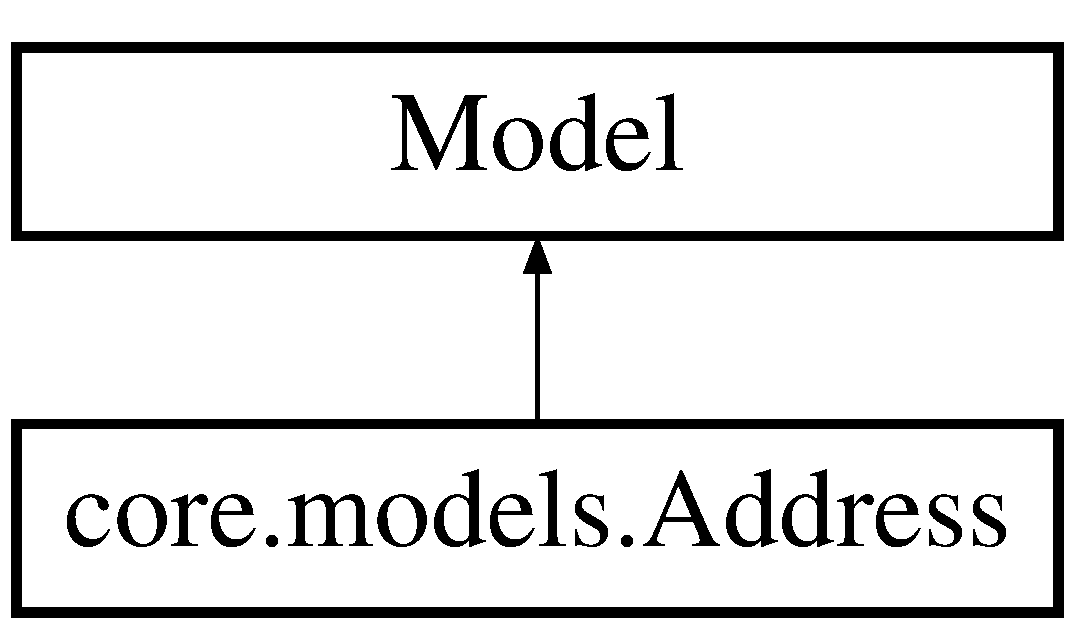
\includegraphics[height=2.000000cm]{classcore_1_1models_1_1Address}
\end{center}
\end{figure}
\subsection*{Classes}
\begin{DoxyCompactItemize}
\item 
class \hyperlink{classcore_1_1models_1_1Address_1_1Meta}{Meta}
\end{DoxyCompactItemize}
\subsection*{Public Member Functions}
\begin{DoxyCompactItemize}
\item 
def \hyperlink{classcore_1_1models_1_1Address_ae7662f36c945c920d731c7a6f0eebdf1}{\-\_\-\-\_\-unicode\-\_\-\-\_\-}
\item 
def \hyperlink{classcore_1_1models_1_1Address_a087d6a195a42b5568b0bd45f6a68723e}{save}
\begin{DoxyCompactList}\small\item\em Custom save method. \end{DoxyCompactList}\item 
def \hyperlink{classcore_1_1models_1_1Address_a118bcbfcb691e9dd708ce2abd3d1dca4}{get\-\_\-seo}
\begin{DoxyCompactList}\small\item\em Get seo link. \end{DoxyCompactList}\end{DoxyCompactItemize}
\subsection*{Public Attributes}
\begin{DoxyCompactItemize}
\item 
\hyperlink{classcore_1_1models_1_1Address_a5ebbca47356580cd05088f58d24d025c}{key\-\_\-name}
\end{DoxyCompactItemize}
\subsection*{Static Public Attributes}
\begin{DoxyCompactItemize}
\item 
tuple \hyperlink{classcore_1_1models_1_1Address_a7d9c715a5bfb018bfc9ca178d91b6b8f}{first\-\_\-name} = dmodels.\-Char\-Field(max\-\_\-length=255, null=True, blank=True)
\item 
tuple \hyperlink{classcore_1_1models_1_1Address_abafe62dc9d25c167398a989a22caee51}{last\-\_\-name} = dmodels.\-Char\-Field(max\-\_\-length=255, null=True, blank=True)
\item 
tuple \hyperlink{classcore_1_1models_1_1Address_a972fdb0ba26470757d213bdb6f140402}{address} = dmodels.\-Char\-Field(max\-\_\-length=255)
\begin{DoxyCompactList}\small\item\em \hyperlink{classcore_1_1models_1_1Address}{Address} address. \end{DoxyCompactList}\item 
tuple \hyperlink{classcore_1_1models_1_1Address_af65d2b194530748ef11ea7f79606cc0d}{address2} = dmodels.\-Char\-Field(max\-\_\-length=255, null=True, blank=True)
\item 
tuple \hyperlink{classcore_1_1models_1_1Address_ac5519e5d6f43f88d8d7c24f4d3439928}{city} = dmodels.\-Char\-Field(max\-\_\-length=255, db\-\_\-index=True)
\begin{DoxyCompactList}\small\item\em \hyperlink{classcore_1_1models_1_1Address}{Address} city. \end{DoxyCompactList}\item 
tuple \hyperlink{classcore_1_1models_1_1Address_affbd91eecd5cf5488103ea1efc16100d}{postcode} = dmodels.\-Char\-Field(max\-\_\-length=64)
\begin{DoxyCompactList}\small\item\em \hyperlink{classcore_1_1models_1_1Address}{Address} postcode. \end{DoxyCompactList}\item 
tuple \hyperlink{classcore_1_1models_1_1Address_a46997a17a6397d68ffb8e0c9e5244c1f}{country} = dmodels.\-Foreign\-Key(\hyperlink{classcore_1_1models_1_1Country}{Country}, null=True, blank=True, db\-\_\-index=True)
\begin{DoxyCompactList}\small\item\em Linked country to address. \end{DoxyCompactList}\end{DoxyCompactItemize}


\subsection{Detailed Description}
\hyperlink{classcore_1_1models_1_1Address}{Address}. 

\hyperlink{classcore_1_1models_1_1User}{User} address 

\subsection{Member Function Documentation}
\hypertarget{classcore_1_1models_1_1Address_ae7662f36c945c920d731c7a6f0eebdf1}{\index{core\-::models\-::\-Address@{core\-::models\-::\-Address}!\-\_\-\-\_\-unicode\-\_\-\-\_\-@{\-\_\-\-\_\-unicode\-\_\-\-\_\-}}
\index{\-\_\-\-\_\-unicode\-\_\-\-\_\-@{\-\_\-\-\_\-unicode\-\_\-\-\_\-}!core::models::Address@{core\-::models\-::\-Address}}
\subsubsection[{\-\_\-\-\_\-unicode\-\_\-\-\_\-}]{\setlength{\rightskip}{0pt plus 5cm}def core.\-models.\-Address.\-\_\-\-\_\-unicode\-\_\-\-\_\- (
\begin{DoxyParamCaption}
\item[{}]{self}
\end{DoxyParamCaption}
)}}\label{classcore_1_1models_1_1Address_ae7662f36c945c920d731c7a6f0eebdf1}
\hypertarget{classcore_1_1models_1_1Address_a118bcbfcb691e9dd708ce2abd3d1dca4}{\index{core\-::models\-::\-Address@{core\-::models\-::\-Address}!get\-\_\-seo@{get\-\_\-seo}}
\index{get\-\_\-seo@{get\-\_\-seo}!core::models::Address@{core\-::models\-::\-Address}}
\subsubsection[{get\-\_\-seo}]{\setlength{\rightskip}{0pt plus 5cm}def core.\-models.\-Address.\-get\-\_\-seo (
\begin{DoxyParamCaption}
\item[{}]{self}
\end{DoxyParamCaption}
)}}\label{classcore_1_1models_1_1Address_a118bcbfcb691e9dd708ce2abd3d1dca4}


Get seo link. 

\hypertarget{classcore_1_1models_1_1Address_a087d6a195a42b5568b0bd45f6a68723e}{\index{core\-::models\-::\-Address@{core\-::models\-::\-Address}!save@{save}}
\index{save@{save}!core::models::Address@{core\-::models\-::\-Address}}
\subsubsection[{save}]{\setlength{\rightskip}{0pt plus 5cm}def core.\-models.\-Address.\-save (
\begin{DoxyParamCaption}
\item[{}]{self, }
\item[{}]{force\-\_\-insert = {\ttfamily False}, }
\item[{}]{force\-\_\-update = {\ttfamily False}, }
\item[{}]{using = {\ttfamily None}, }
\item[{}]{update\-\_\-fields = {\ttfamily None}}
\end{DoxyParamCaption}
)}}\label{classcore_1_1models_1_1Address_a087d6a195a42b5568b0bd45f6a68723e}


Custom save method. 



\subsection{Member Data Documentation}
\hypertarget{classcore_1_1models_1_1Address_a972fdb0ba26470757d213bdb6f140402}{\index{core\-::models\-::\-Address@{core\-::models\-::\-Address}!address@{address}}
\index{address@{address}!core::models::Address@{core\-::models\-::\-Address}}
\subsubsection[{address}]{\setlength{\rightskip}{0pt plus 5cm}core.\-models.\-Address.\-address = dmodels.\-Char\-Field(max\-\_\-length=255)\hspace{0.3cm}{\ttfamily [static]}}}\label{classcore_1_1models_1_1Address_a972fdb0ba26470757d213bdb6f140402}


\hyperlink{classcore_1_1models_1_1Address}{Address} address. 

\hypertarget{classcore_1_1models_1_1Address_af65d2b194530748ef11ea7f79606cc0d}{\index{core\-::models\-::\-Address@{core\-::models\-::\-Address}!address2@{address2}}
\index{address2@{address2}!core::models::Address@{core\-::models\-::\-Address}}
\subsubsection[{address2}]{\setlength{\rightskip}{0pt plus 5cm}tuple core.\-models.\-Address.\-address2 = dmodels.\-Char\-Field(max\-\_\-length=255, null=True, blank=True)\hspace{0.3cm}{\ttfamily [static]}}}\label{classcore_1_1models_1_1Address_af65d2b194530748ef11ea7f79606cc0d}
\hypertarget{classcore_1_1models_1_1Address_ac5519e5d6f43f88d8d7c24f4d3439928}{\index{core\-::models\-::\-Address@{core\-::models\-::\-Address}!city@{city}}
\index{city@{city}!core::models::Address@{core\-::models\-::\-Address}}
\subsubsection[{city}]{\setlength{\rightskip}{0pt plus 5cm}core.\-models.\-Address.\-city = dmodels.\-Char\-Field(max\-\_\-length=255, db\-\_\-index=True)\hspace{0.3cm}{\ttfamily [static]}}}\label{classcore_1_1models_1_1Address_ac5519e5d6f43f88d8d7c24f4d3439928}


\hyperlink{classcore_1_1models_1_1Address}{Address} city. 

\hypertarget{classcore_1_1models_1_1Address_a46997a17a6397d68ffb8e0c9e5244c1f}{\index{core\-::models\-::\-Address@{core\-::models\-::\-Address}!country@{country}}
\index{country@{country}!core::models::Address@{core\-::models\-::\-Address}}
\subsubsection[{country}]{\setlength{\rightskip}{0pt plus 5cm}core.\-models.\-Address.\-country = dmodels.\-Foreign\-Key({\bf Country}, null=True, blank=True, db\-\_\-index=True)\hspace{0.3cm}{\ttfamily [static]}}}\label{classcore_1_1models_1_1Address_a46997a17a6397d68ffb8e0c9e5244c1f}


Linked country to address. 

\hypertarget{classcore_1_1models_1_1Address_a7d9c715a5bfb018bfc9ca178d91b6b8f}{\index{core\-::models\-::\-Address@{core\-::models\-::\-Address}!first\-\_\-name@{first\-\_\-name}}
\index{first\-\_\-name@{first\-\_\-name}!core::models::Address@{core\-::models\-::\-Address}}
\subsubsection[{first\-\_\-name}]{\setlength{\rightskip}{0pt plus 5cm}tuple core.\-models.\-Address.\-first\-\_\-name = dmodels.\-Char\-Field(max\-\_\-length=255, null=True, blank=True)\hspace{0.3cm}{\ttfamily [static]}}}\label{classcore_1_1models_1_1Address_a7d9c715a5bfb018bfc9ca178d91b6b8f}
\hypertarget{classcore_1_1models_1_1Address_a5ebbca47356580cd05088f58d24d025c}{\index{core\-::models\-::\-Address@{core\-::models\-::\-Address}!key\-\_\-name@{key\-\_\-name}}
\index{key\-\_\-name@{key\-\_\-name}!core::models::Address@{core\-::models\-::\-Address}}
\subsubsection[{key\-\_\-name}]{\setlength{\rightskip}{0pt plus 5cm}core.\-models.\-Address.\-key\-\_\-name}}\label{classcore_1_1models_1_1Address_a5ebbca47356580cd05088f58d24d025c}
\hypertarget{classcore_1_1models_1_1Address_abafe62dc9d25c167398a989a22caee51}{\index{core\-::models\-::\-Address@{core\-::models\-::\-Address}!last\-\_\-name@{last\-\_\-name}}
\index{last\-\_\-name@{last\-\_\-name}!core::models::Address@{core\-::models\-::\-Address}}
\subsubsection[{last\-\_\-name}]{\setlength{\rightskip}{0pt plus 5cm}tuple core.\-models.\-Address.\-last\-\_\-name = dmodels.\-Char\-Field(max\-\_\-length=255, null=True, blank=True)\hspace{0.3cm}{\ttfamily [static]}}}\label{classcore_1_1models_1_1Address_abafe62dc9d25c167398a989a22caee51}
\hypertarget{classcore_1_1models_1_1Address_affbd91eecd5cf5488103ea1efc16100d}{\index{core\-::models\-::\-Address@{core\-::models\-::\-Address}!postcode@{postcode}}
\index{postcode@{postcode}!core::models::Address@{core\-::models\-::\-Address}}
\subsubsection[{postcode}]{\setlength{\rightskip}{0pt plus 5cm}core.\-models.\-Address.\-postcode = dmodels.\-Char\-Field(max\-\_\-length=64)\hspace{0.3cm}{\ttfamily [static]}}}\label{classcore_1_1models_1_1Address_affbd91eecd5cf5488103ea1efc16100d}


\hyperlink{classcore_1_1models_1_1Address}{Address} postcode. 



The documentation for this class was generated from the following file\-:\begin{DoxyCompactItemize}
\item 
/wepo/core/\hyperlink{models_8py}{models.\-py}\end{DoxyCompactItemize}

\hypertarget{classcore_1_1management_1_1commands_1_1unit_1_1Command}{\section{core.\-management.\-commands.\-unit.\-Command Class Reference}
\label{classcore_1_1management_1_1commands_1_1unit_1_1Command}\index{core.\-management.\-commands.\-unit.\-Command@{core.\-management.\-commands.\-unit.\-Command}}
}


Wepo unit tests.  


Inheritance diagram for core.\-management.\-commands.\-unit.\-Command\-:\begin{figure}[H]
\begin{center}
\leavevmode
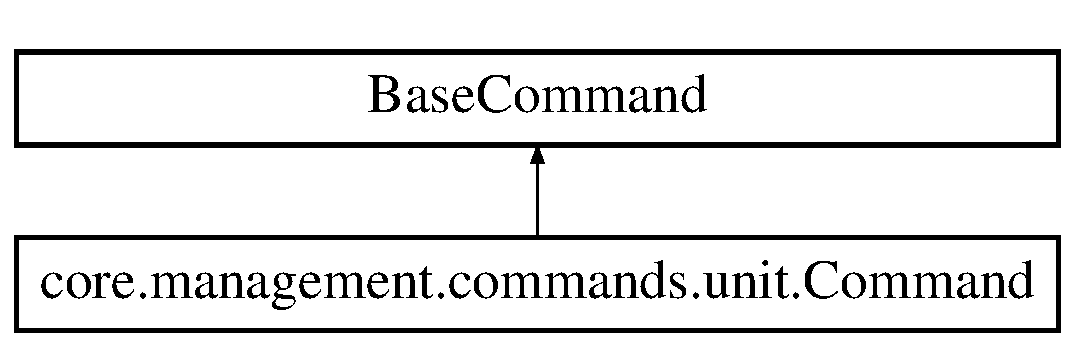
\includegraphics[height=2.000000cm]{classcore_1_1management_1_1commands_1_1unit_1_1Command}
\end{center}
\end{figure}
\subsection*{Public Member Functions}
\begin{DoxyCompactItemize}
\item 
def \hyperlink{classcore_1_1management_1_1commands_1_1unit_1_1Command_a0f9ceb6f7eb04fbcad81d371a8cac8f9}{handle}
\begin{DoxyCompactList}\small\item\em \hyperlink{classcore_1_1management_1_1commands_1_1unit_1_1Command}{Command} handler. \end{DoxyCompactList}\end{DoxyCompactItemize}
\subsection*{Static Public Attributes}
\begin{DoxyCompactItemize}
\item 
\hyperlink{classcore_1_1management_1_1commands_1_1unit_1_1Command_a72c89b56acfcfbda87b8401adf0efa54}{option\-\_\-list} = Base\-Command.\-option\-\_\-list
\item 
string \hyperlink{classcore_1_1management_1_1commands_1_1unit_1_1Command_afa3ee03895753060f709326a6a403651}{help} = 'Unit tests.'
\end{DoxyCompactItemize}


\subsection{Detailed Description}
Wepo unit tests. 

\subsection{Member Function Documentation}
\hypertarget{classcore_1_1management_1_1commands_1_1unit_1_1Command_a0f9ceb6f7eb04fbcad81d371a8cac8f9}{\index{core\-::management\-::commands\-::unit\-::\-Command@{core\-::management\-::commands\-::unit\-::\-Command}!handle@{handle}}
\index{handle@{handle}!core::management::commands::unit::Command@{core\-::management\-::commands\-::unit\-::\-Command}}
\subsubsection[{handle}]{\setlength{\rightskip}{0pt plus 5cm}def core.\-management.\-commands.\-unit.\-Command.\-handle (
\begin{DoxyParamCaption}
\item[{}]{self, }
\item[{}]{args, }
\item[{}]{options}
\end{DoxyParamCaption}
)}}\label{classcore_1_1management_1_1commands_1_1unit_1_1Command_a0f9ceb6f7eb04fbcad81d371a8cac8f9}


\hyperlink{classcore_1_1management_1_1commands_1_1unit_1_1Command}{Command} handler. 


\begin{DoxyParams}{Parameters}
{\em args} & Extra arguments passed to the handler \\
\hline
{\em options} & Available options with command \\
\hline
\end{DoxyParams}


\subsection{Member Data Documentation}
\hypertarget{classcore_1_1management_1_1commands_1_1unit_1_1Command_afa3ee03895753060f709326a6a403651}{\index{core\-::management\-::commands\-::unit\-::\-Command@{core\-::management\-::commands\-::unit\-::\-Command}!help@{help}}
\index{help@{help}!core::management::commands::unit::Command@{core\-::management\-::commands\-::unit\-::\-Command}}
\subsubsection[{help}]{\setlength{\rightskip}{0pt plus 5cm}string core.\-management.\-commands.\-unit.\-Command.\-help = 'Unit tests.'\hspace{0.3cm}{\ttfamily [static]}}}\label{classcore_1_1management_1_1commands_1_1unit_1_1Command_afa3ee03895753060f709326a6a403651}
\hypertarget{classcore_1_1management_1_1commands_1_1unit_1_1Command_a72c89b56acfcfbda87b8401adf0efa54}{\index{core\-::management\-::commands\-::unit\-::\-Command@{core\-::management\-::commands\-::unit\-::\-Command}!option\-\_\-list@{option\-\_\-list}}
\index{option\-\_\-list@{option\-\_\-list}!core::management::commands::unit::Command@{core\-::management\-::commands\-::unit\-::\-Command}}
\subsubsection[{option\-\_\-list}]{\setlength{\rightskip}{0pt plus 5cm}core.\-management.\-commands.\-unit.\-Command.\-option\-\_\-list = Base\-Command.\-option\-\_\-list\hspace{0.3cm}{\ttfamily [static]}}}\label{classcore_1_1management_1_1commands_1_1unit_1_1Command_a72c89b56acfcfbda87b8401adf0efa54}


The documentation for this class was generated from the following file\-:\begin{DoxyCompactItemize}
\item 
/wepo/core/management/commands/\hyperlink{unit_8py}{unit.\-py}\end{DoxyCompactItemize}

\hypertarget{classcore_1_1management_1_1commands_1_1sync_1_1Command}{\section{core.\-management.\-commands.\-sync.\-Command Class Reference}
\label{classcore_1_1management_1_1commands_1_1sync_1_1Command}\index{core.\-management.\-commands.\-sync.\-Command@{core.\-management.\-commands.\-sync.\-Command}}
}


Wepo sync db for installed apps.  


Inheritance diagram for core.\-management.\-commands.\-sync.\-Command\-:\begin{figure}[H]
\begin{center}
\leavevmode
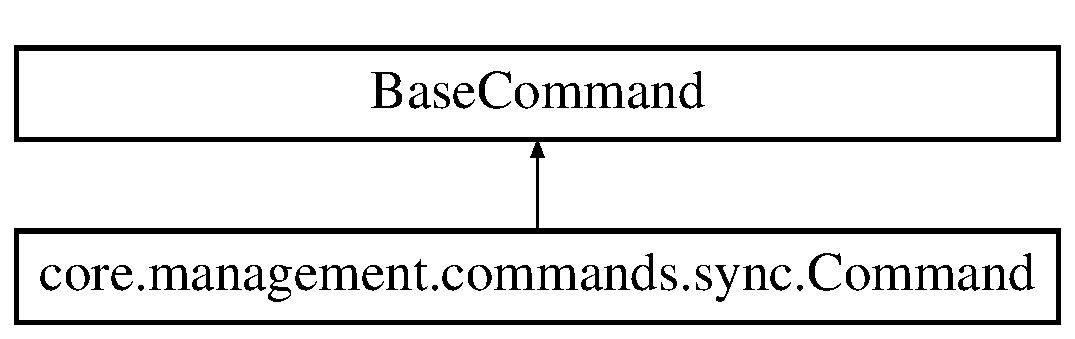
\includegraphics[height=2.000000cm]{classcore_1_1management_1_1commands_1_1sync_1_1Command}
\end{center}
\end{figure}
\subsection*{Public Member Functions}
\begin{DoxyCompactItemize}
\item 
def \hyperlink{classcore_1_1management_1_1commands_1_1sync_1_1Command_a3af67429e0e048166f4c2b551135456d}{handle}
\begin{DoxyCompactList}\small\item\em \hyperlink{classcore_1_1management_1_1commands_1_1sync_1_1Command}{Command} handler. \end{DoxyCompactList}\item 
def \hyperlink{classcore_1_1management_1_1commands_1_1sync_1_1Command_a84af1ad11a080e35037ca14f7042a085}{import\-\_\-from\-\_\-all}
\begin{DoxyCompactList}\small\item\em Import fixtures from all installed apps. \end{DoxyCompactList}\end{DoxyCompactItemize}
\subsection*{Static Public Attributes}
\begin{DoxyCompactItemize}
\item 
\hyperlink{classcore_1_1management_1_1commands_1_1sync_1_1Command_aa3316701d237502a5f8c7d5ddf038613}{option\-\_\-list} = Base\-Command.\-option\-\_\-list
\begin{DoxyCompactList}\small\item\em Options. \end{DoxyCompactList}\item 
string \hyperlink{classcore_1_1management_1_1commands_1_1sync_1_1Command_a6efa96168e0103973ca2824e8a51e5ad}{help} = 'Import fixtures from installed applications.'
\end{DoxyCompactItemize}


\subsection{Detailed Description}
Wepo sync db for installed apps. 

\subsection{Member Function Documentation}
\hypertarget{classcore_1_1management_1_1commands_1_1sync_1_1Command_a3af67429e0e048166f4c2b551135456d}{\index{core\-::management\-::commands\-::sync\-::\-Command@{core\-::management\-::commands\-::sync\-::\-Command}!handle@{handle}}
\index{handle@{handle}!core::management::commands::sync::Command@{core\-::management\-::commands\-::sync\-::\-Command}}
\subsubsection[{handle}]{\setlength{\rightskip}{0pt plus 5cm}def core.\-management.\-commands.\-sync.\-Command.\-handle (
\begin{DoxyParamCaption}
\item[{}]{self, }
\item[{}]{args, }
\item[{}]{options}
\end{DoxyParamCaption}
)}}\label{classcore_1_1management_1_1commands_1_1sync_1_1Command_a3af67429e0e048166f4c2b551135456d}


\hyperlink{classcore_1_1management_1_1commands_1_1sync_1_1Command}{Command} handler. 


\begin{DoxyParams}{Parameters}
{\em args} & Extra arguments passed to the handler \\
\hline
{\em options} & Available options with command \\
\hline
\end{DoxyParams}
\hypertarget{classcore_1_1management_1_1commands_1_1sync_1_1Command_a84af1ad11a080e35037ca14f7042a085}{\index{core\-::management\-::commands\-::sync\-::\-Command@{core\-::management\-::commands\-::sync\-::\-Command}!import\-\_\-from\-\_\-all@{import\-\_\-from\-\_\-all}}
\index{import\-\_\-from\-\_\-all@{import\-\_\-from\-\_\-all}!core::management::commands::sync::Command@{core\-::management\-::commands\-::sync\-::\-Command}}
\subsubsection[{import\-\_\-from\-\_\-all}]{\setlength{\rightskip}{0pt plus 5cm}def core.\-management.\-commands.\-sync.\-Command.\-import\-\_\-from\-\_\-all (
\begin{DoxyParamCaption}
\item[{}]{self}
\end{DoxyParamCaption}
)}}\label{classcore_1_1management_1_1commands_1_1sync_1_1Command_a84af1ad11a080e35037ca14f7042a085}


Import fixtures from all installed apps. 



\subsection{Member Data Documentation}
\hypertarget{classcore_1_1management_1_1commands_1_1sync_1_1Command_a6efa96168e0103973ca2824e8a51e5ad}{\index{core\-::management\-::commands\-::sync\-::\-Command@{core\-::management\-::commands\-::sync\-::\-Command}!help@{help}}
\index{help@{help}!core::management::commands::sync::Command@{core\-::management\-::commands\-::sync\-::\-Command}}
\subsubsection[{help}]{\setlength{\rightskip}{0pt plus 5cm}string core.\-management.\-commands.\-sync.\-Command.\-help = 'Import fixtures from installed applications.'\hspace{0.3cm}{\ttfamily [static]}}}\label{classcore_1_1management_1_1commands_1_1sync_1_1Command_a6efa96168e0103973ca2824e8a51e5ad}
\hypertarget{classcore_1_1management_1_1commands_1_1sync_1_1Command_aa3316701d237502a5f8c7d5ddf038613}{\index{core\-::management\-::commands\-::sync\-::\-Command@{core\-::management\-::commands\-::sync\-::\-Command}!option\-\_\-list@{option\-\_\-list}}
\index{option\-\_\-list@{option\-\_\-list}!core::management::commands::sync::Command@{core\-::management\-::commands\-::sync\-::\-Command}}
\subsubsection[{option\-\_\-list}]{\setlength{\rightskip}{0pt plus 5cm}core.\-management.\-commands.\-sync.\-Command.\-option\-\_\-list = Base\-Command.\-option\-\_\-list\hspace{0.3cm}{\ttfamily [static]}}}\label{classcore_1_1management_1_1commands_1_1sync_1_1Command_aa3316701d237502a5f8c7d5ddf038613}


Options. 



The documentation for this class was generated from the following file\-:\begin{DoxyCompactItemize}
\item 
/wepo/core/management/commands/\hyperlink{sync_8py}{sync.\-py}\end{DoxyCompactItemize}

\hypertarget{classcore_1_1models_1_1Country}{\section{core.\-models.\-Country Class Reference}
\label{classcore_1_1models_1_1Country}\index{core.\-models.\-Country@{core.\-models.\-Country}}
}


\hyperlink{classcore_1_1models_1_1Country}{Country}.  


Inheritance diagram for core.\-models.\-Country\-:\begin{figure}[H]
\begin{center}
\leavevmode
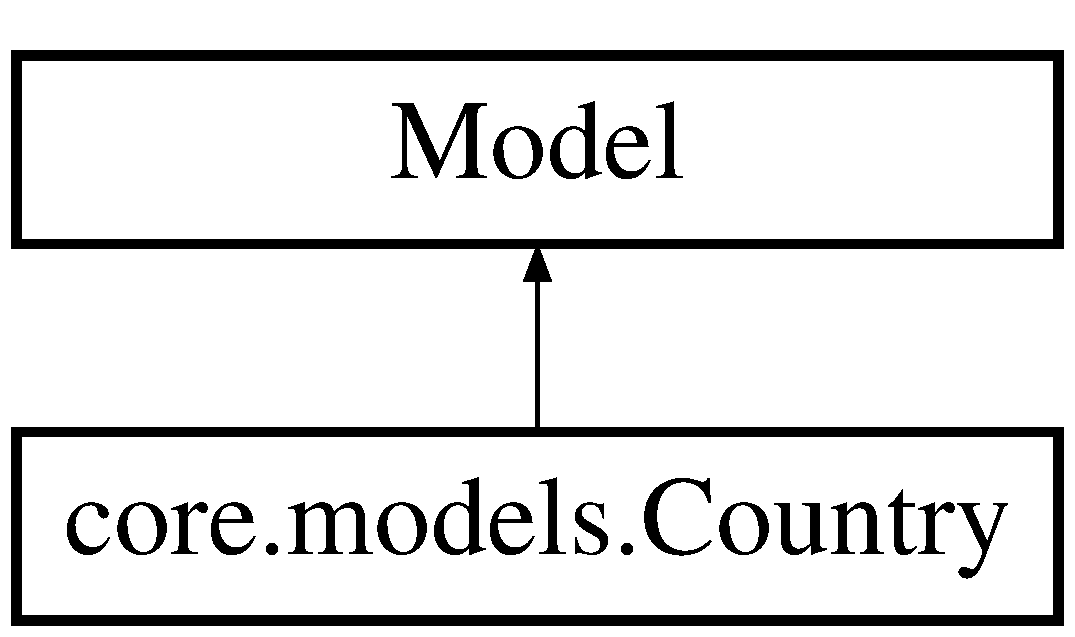
\includegraphics[height=2.000000cm]{classcore_1_1models_1_1Country}
\end{center}
\end{figure}
\subsection*{Classes}
\begin{DoxyCompactItemize}
\item 
class \hyperlink{classcore_1_1models_1_1Country_1_1Meta}{Meta}
\end{DoxyCompactItemize}
\subsection*{Public Member Functions}
\begin{DoxyCompactItemize}
\item 
def \hyperlink{classcore_1_1models_1_1Country_a76f03de6f967f84e57361796365e9a81}{\-\_\-\-\_\-unicode\-\_\-\-\_\-}
\item 
def \hyperlink{classcore_1_1models_1_1Country_a62cf8891c894c8c6aa39bb022b078515}{save}
\begin{DoxyCompactList}\small\item\em Custom save method. \end{DoxyCompactList}\item 
def \hyperlink{classcore_1_1models_1_1Country_aed7e5c275696380b6ef1867bf5c915f4}{get\-\_\-seo}
\begin{DoxyCompactList}\small\item\em Get seo link. \end{DoxyCompactList}\end{DoxyCompactItemize}
\subsection*{Public Attributes}
\begin{DoxyCompactItemize}
\item 
\hyperlink{classcore_1_1models_1_1Country_ac21ce3fc1459b072b4fc49d53c525867}{key\-\_\-name}
\end{DoxyCompactItemize}
\subsection*{Static Public Attributes}
\begin{DoxyCompactItemize}
\item 
tuple \hyperlink{classcore_1_1models_1_1Country_abadb165c9cb65ad347d076a20c1d7690}{name} = dmodels.\-Char\-Field(max\-\_\-length=64)
\begin{DoxyCompactList}\small\item\em \hyperlink{classcore_1_1models_1_1Country}{Country} name. \end{DoxyCompactList}\item 
tuple \hyperlink{classcore_1_1models_1_1Country_a0e69789f36a5e3ae61532a9cf69763a5}{code} = dmodels.\-Char\-Field(max\-\_\-length=2, db\-\_\-index=True)
\begin{DoxyCompactList}\small\item\em Code of the language by I\-S\-O 639-\/1 Code standard (Upgradeable to I\-S\-O 639-\/2 Code standard) \end{DoxyCompactList}\item 
tuple \hyperlink{classcore_1_1models_1_1Country_ac21ce3fc1459b072b4fc49d53c525867}{key\-\_\-name} = dmodels.\-Char\-Field(max\-\_\-length=64, db\-\_\-index=True)
\begin{DoxyCompactList}\small\item\em Unique identifier of the country. \end{DoxyCompactList}\end{DoxyCompactItemize}


\subsection{Detailed Description}
\hyperlink{classcore_1_1models_1_1Country}{Country}. 

Countries 

\subsection{Member Function Documentation}
\hypertarget{classcore_1_1models_1_1Country_a76f03de6f967f84e57361796365e9a81}{\index{core\-::models\-::\-Country@{core\-::models\-::\-Country}!\-\_\-\-\_\-unicode\-\_\-\-\_\-@{\-\_\-\-\_\-unicode\-\_\-\-\_\-}}
\index{\-\_\-\-\_\-unicode\-\_\-\-\_\-@{\-\_\-\-\_\-unicode\-\_\-\-\_\-}!core::models::Country@{core\-::models\-::\-Country}}
\subsubsection[{\-\_\-\-\_\-unicode\-\_\-\-\_\-}]{\setlength{\rightskip}{0pt plus 5cm}def core.\-models.\-Country.\-\_\-\-\_\-unicode\-\_\-\-\_\- (
\begin{DoxyParamCaption}
\item[{}]{self}
\end{DoxyParamCaption}
)}}\label{classcore_1_1models_1_1Country_a76f03de6f967f84e57361796365e9a81}
\hypertarget{classcore_1_1models_1_1Country_aed7e5c275696380b6ef1867bf5c915f4}{\index{core\-::models\-::\-Country@{core\-::models\-::\-Country}!get\-\_\-seo@{get\-\_\-seo}}
\index{get\-\_\-seo@{get\-\_\-seo}!core::models::Country@{core\-::models\-::\-Country}}
\subsubsection[{get\-\_\-seo}]{\setlength{\rightskip}{0pt plus 5cm}def core.\-models.\-Country.\-get\-\_\-seo (
\begin{DoxyParamCaption}
\item[{}]{self}
\end{DoxyParamCaption}
)}}\label{classcore_1_1models_1_1Country_aed7e5c275696380b6ef1867bf5c915f4}


Get seo link. 

\hypertarget{classcore_1_1models_1_1Country_a62cf8891c894c8c6aa39bb022b078515}{\index{core\-::models\-::\-Country@{core\-::models\-::\-Country}!save@{save}}
\index{save@{save}!core::models::Country@{core\-::models\-::\-Country}}
\subsubsection[{save}]{\setlength{\rightskip}{0pt plus 5cm}def core.\-models.\-Country.\-save (
\begin{DoxyParamCaption}
\item[{}]{self, }
\item[{}]{force\-\_\-insert = {\ttfamily False}, }
\item[{}]{force\-\_\-update = {\ttfamily False}, }
\item[{}]{using = {\ttfamily None}, }
\item[{}]{update\-\_\-fields = {\ttfamily None}}
\end{DoxyParamCaption}
)}}\label{classcore_1_1models_1_1Country_a62cf8891c894c8c6aa39bb022b078515}


Custom save method. 



\subsection{Member Data Documentation}
\hypertarget{classcore_1_1models_1_1Country_a0e69789f36a5e3ae61532a9cf69763a5}{\index{core\-::models\-::\-Country@{core\-::models\-::\-Country}!code@{code}}
\index{code@{code}!core::models::Country@{core\-::models\-::\-Country}}
\subsubsection[{code}]{\setlength{\rightskip}{0pt plus 5cm}core.\-models.\-Country.\-code = dmodels.\-Char\-Field(max\-\_\-length=2, db\-\_\-index=True)\hspace{0.3cm}{\ttfamily [static]}}}\label{classcore_1_1models_1_1Country_a0e69789f36a5e3ae61532a9cf69763a5}


Code of the language by I\-S\-O 639-\/1 Code standard (Upgradeable to I\-S\-O 639-\/2 Code standard) 

\hypertarget{classcore_1_1models_1_1Country_ac21ce3fc1459b072b4fc49d53c525867}{\index{core\-::models\-::\-Country@{core\-::models\-::\-Country}!key\-\_\-name@{key\-\_\-name}}
\index{key\-\_\-name@{key\-\_\-name}!core::models::Country@{core\-::models\-::\-Country}}
\subsubsection[{key\-\_\-name}]{\setlength{\rightskip}{0pt plus 5cm}core.\-models.\-Country.\-key\-\_\-name = dmodels.\-Char\-Field(max\-\_\-length=64, db\-\_\-index=True)\hspace{0.3cm}{\ttfamily [static]}}}\label{classcore_1_1models_1_1Country_ac21ce3fc1459b072b4fc49d53c525867}


Unique identifier of the country. 

\hypertarget{classcore_1_1models_1_1Country_ac21ce3fc1459b072b4fc49d53c525867}{\index{core\-::models\-::\-Country@{core\-::models\-::\-Country}!key\-\_\-name@{key\-\_\-name}}
\index{key\-\_\-name@{key\-\_\-name}!core::models::Country@{core\-::models\-::\-Country}}
\subsubsection[{key\-\_\-name}]{\setlength{\rightskip}{0pt plus 5cm}core.\-models.\-Country.\-key\-\_\-name}}\label{classcore_1_1models_1_1Country_ac21ce3fc1459b072b4fc49d53c525867}
\hypertarget{classcore_1_1models_1_1Country_abadb165c9cb65ad347d076a20c1d7690}{\index{core\-::models\-::\-Country@{core\-::models\-::\-Country}!name@{name}}
\index{name@{name}!core::models::Country@{core\-::models\-::\-Country}}
\subsubsection[{name}]{\setlength{\rightskip}{0pt plus 5cm}core.\-models.\-Country.\-name = dmodels.\-Char\-Field(max\-\_\-length=64)\hspace{0.3cm}{\ttfamily [static]}}}\label{classcore_1_1models_1_1Country_abadb165c9cb65ad347d076a20c1d7690}


\hyperlink{classcore_1_1models_1_1Country}{Country} name. 



The documentation for this class was generated from the following file\-:\begin{DoxyCompactItemize}
\item 
/wepo/core/\hyperlink{models_8py}{models.\-py}\end{DoxyCompactItemize}

\hypertarget{classcore_1_1models_1_1Directory}{\section{core.\-models.\-Directory Class Reference}
\label{classcore_1_1models_1_1Directory}\index{core.\-models.\-Directory@{core.\-models.\-Directory}}
}


\hyperlink{classcore_1_1models_1_1Directory}{Directory}.  


Inheritance diagram for core.\-models.\-Directory\-:\begin{figure}[H]
\begin{center}
\leavevmode
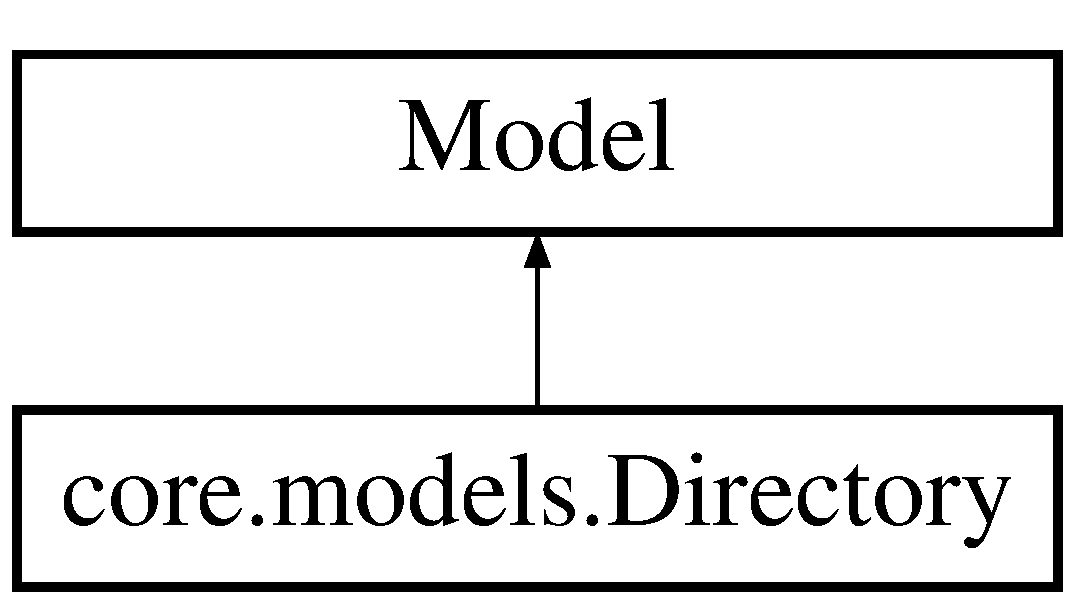
\includegraphics[height=2.000000cm]{classcore_1_1models_1_1Directory}
\end{center}
\end{figure}
\subsection*{Classes}
\begin{DoxyCompactItemize}
\item 
class \hyperlink{classcore_1_1models_1_1Directory_1_1Meta}{Meta}
\end{DoxyCompactItemize}
\subsection*{Public Member Functions}
\begin{DoxyCompactItemize}
\item 
def \hyperlink{classcore_1_1models_1_1Directory_a9ed85c6776b6e77c5b9f42a49f90a6af}{\-\_\-\-\_\-unicode\-\_\-\-\_\-}
\item 
def \hyperlink{classcore_1_1models_1_1Directory_a7c6d03d3fe7f4854dcda4559fc99815a}{save}
\begin{DoxyCompactList}\small\item\em Custom save method. \end{DoxyCompactList}\end{DoxyCompactItemize}
\subsection*{Static Public Attributes}
\begin{DoxyCompactItemize}
\item 
tuple \hyperlink{classcore_1_1models_1_1Directory_a1d5a9f2dd8f591cf1bd6410dee7d3b26}{name} = dmodels.\-Char\-Field(max\-\_\-length=255, db\-\_\-index=True)
\begin{DoxyCompactList}\small\item\em Name of the directory. \end{DoxyCompactList}\item 
tuple \hyperlink{classcore_1_1models_1_1Directory_ad0341e7ba04c23d665cb318ebee17c2b}{parent} = dmodels.\-Foreign\-Key('self', null=True, blank=True)
\begin{DoxyCompactList}\small\item\em \hyperlink{classcore_1_1models_1_1Directory}{Directory} parent. \end{DoxyCompactList}\end{DoxyCompactItemize}


\subsection{Detailed Description}
\hyperlink{classcore_1_1models_1_1Directory}{Directory}. 

\hyperlink{classcore_1_1models_1_1File}{File} directories 

\subsection{Member Function Documentation}
\hypertarget{classcore_1_1models_1_1Directory_a9ed85c6776b6e77c5b9f42a49f90a6af}{\index{core\-::models\-::\-Directory@{core\-::models\-::\-Directory}!\-\_\-\-\_\-unicode\-\_\-\-\_\-@{\-\_\-\-\_\-unicode\-\_\-\-\_\-}}
\index{\-\_\-\-\_\-unicode\-\_\-\-\_\-@{\-\_\-\-\_\-unicode\-\_\-\-\_\-}!core::models::Directory@{core\-::models\-::\-Directory}}
\subsubsection[{\-\_\-\-\_\-unicode\-\_\-\-\_\-}]{\setlength{\rightskip}{0pt plus 5cm}def core.\-models.\-Directory.\-\_\-\-\_\-unicode\-\_\-\-\_\- (
\begin{DoxyParamCaption}
\item[{}]{self}
\end{DoxyParamCaption}
)}}\label{classcore_1_1models_1_1Directory_a9ed85c6776b6e77c5b9f42a49f90a6af}
\hypertarget{classcore_1_1models_1_1Directory_a7c6d03d3fe7f4854dcda4559fc99815a}{\index{core\-::models\-::\-Directory@{core\-::models\-::\-Directory}!save@{save}}
\index{save@{save}!core::models::Directory@{core\-::models\-::\-Directory}}
\subsubsection[{save}]{\setlength{\rightskip}{0pt plus 5cm}def core.\-models.\-Directory.\-save (
\begin{DoxyParamCaption}
\item[{}]{self, }
\item[{}]{force\-\_\-insert = {\ttfamily False}, }
\item[{}]{force\-\_\-update = {\ttfamily False}, }
\item[{}]{using = {\ttfamily None}, }
\item[{}]{update\-\_\-fields = {\ttfamily None}}
\end{DoxyParamCaption}
)}}\label{classcore_1_1models_1_1Directory_a7c6d03d3fe7f4854dcda4559fc99815a}


Custom save method. 



\subsection{Member Data Documentation}
\hypertarget{classcore_1_1models_1_1Directory_a1d5a9f2dd8f591cf1bd6410dee7d3b26}{\index{core\-::models\-::\-Directory@{core\-::models\-::\-Directory}!name@{name}}
\index{name@{name}!core::models::Directory@{core\-::models\-::\-Directory}}
\subsubsection[{name}]{\setlength{\rightskip}{0pt plus 5cm}core.\-models.\-Directory.\-name = dmodels.\-Char\-Field(max\-\_\-length=255, db\-\_\-index=True)\hspace{0.3cm}{\ttfamily [static]}}}\label{classcore_1_1models_1_1Directory_a1d5a9f2dd8f591cf1bd6410dee7d3b26}


Name of the directory. 

\hypertarget{classcore_1_1models_1_1Directory_ad0341e7ba04c23d665cb318ebee17c2b}{\index{core\-::models\-::\-Directory@{core\-::models\-::\-Directory}!parent@{parent}}
\index{parent@{parent}!core::models::Directory@{core\-::models\-::\-Directory}}
\subsubsection[{parent}]{\setlength{\rightskip}{0pt plus 5cm}core.\-models.\-Directory.\-parent = dmodels.\-Foreign\-Key('self', null=True, blank=True)\hspace{0.3cm}{\ttfamily [static]}}}\label{classcore_1_1models_1_1Directory_ad0341e7ba04c23d665cb318ebee17c2b}


\hyperlink{classcore_1_1models_1_1Directory}{Directory} parent. 



The documentation for this class was generated from the following file\-:\begin{DoxyCompactItemize}
\item 
/wepo/core/\hyperlink{models_8py}{models.\-py}\end{DoxyCompactItemize}

\hypertarget{classcore_1_1helper_1_1exception__help_1_1Error}{\section{core.\-helper.\-exception\-\_\-help.\-Error Class Reference}
\label{classcore_1_1helper_1_1exception__help_1_1Error}\index{core.\-helper.\-exception\-\_\-help.\-Error@{core.\-helper.\-exception\-\_\-help.\-Error}}
}


Base class for exceptions in this module.  


Inheritance diagram for core.\-helper.\-exception\-\_\-help.\-Error\-:\begin{figure}[H]
\begin{center}
\leavevmode
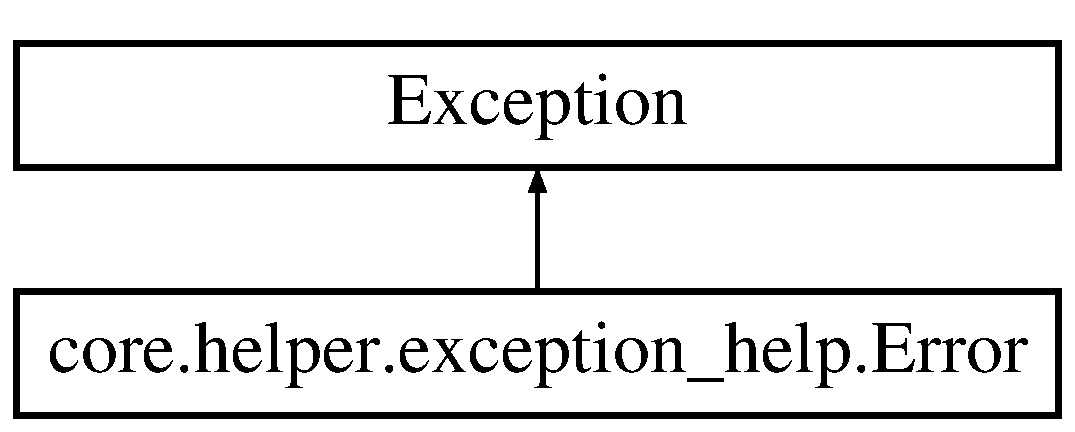
\includegraphics[height=2.000000cm]{classcore_1_1helper_1_1exception__help_1_1Error}
\end{center}
\end{figure}


\subsection{Detailed Description}
Base class for exceptions in this module. 

The documentation for this class was generated from the following file\-:\begin{DoxyCompactItemize}
\item 
/wepo/core/helper/\hyperlink{exception__help_8py}{exception\-\_\-help.\-py}\end{DoxyCompactItemize}

\hypertarget{classcore_1_1decorators_1_1model_1_1field__group}{\section{core.\-decorators.\-model.\-field\-\_\-group Class Reference}
\label{classcore_1_1decorators_1_1model_1_1field__group}\index{core.\-decorators.\-model.\-field\-\_\-group@{core.\-decorators.\-model.\-field\-\_\-group}}
}


Group fields together.  


Inheritance diagram for core.\-decorators.\-model.\-field\-\_\-group\-:\begin{figure}[H]
\begin{center}
\leavevmode
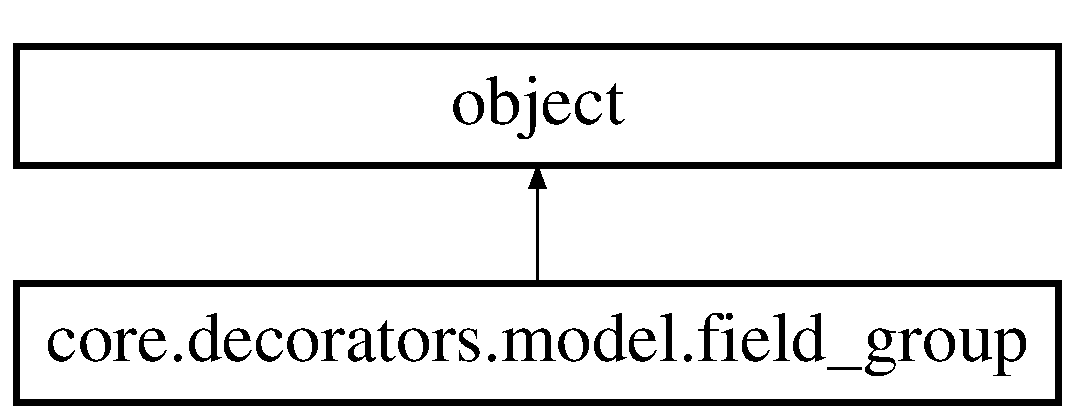
\includegraphics[height=2.000000cm]{classcore_1_1decorators_1_1model_1_1field__group}
\end{center}
\end{figure}
\subsection*{Public Member Functions}
\begin{DoxyCompactItemize}
\item 
def \hyperlink{classcore_1_1decorators_1_1model_1_1field__group_a5339cc227ed382399ebaad81fba6d237}{\-\_\-\-\_\-init\-\_\-\-\_\-}
\begin{DoxyCompactList}\small\item\em Save passed arguments. \end{DoxyCompactList}\item 
def \hyperlink{classcore_1_1decorators_1_1model_1_1field__group_a2d763625dfae687a30ed0ef6337c5a8f}{\-\_\-\-\_\-call\-\_\-\-\_\-}
\begin{DoxyCompactList}\small\item\em Configure field. \end{DoxyCompactList}\end{DoxyCompactItemize}
\subsection*{Public Attributes}
\begin{DoxyCompactItemize}
\item 
\hyperlink{classcore_1_1decorators_1_1model_1_1field__group_a18917138eb13e0aac794921e8b0b01c4}{name}
\item 
\hyperlink{classcore_1_1decorators_1_1model_1_1field__group_a56e0be74f7aa784b96a5d1ee25589f5c}{fields}
\item 
\hyperlink{classcore_1_1decorators_1_1model_1_1field__group_ade67e97a20f107664fd9f4d2fbddab57}{data}
\end{DoxyCompactItemize}


\subsection{Detailed Description}
Group fields together. 


\begin{DoxyParams}{Parameters}
{\em object} & Model which will be configured \\
\hline
\end{DoxyParams}


\subsection{Constructor \& Destructor Documentation}
\hypertarget{classcore_1_1decorators_1_1model_1_1field__group_a5339cc227ed382399ebaad81fba6d237}{\index{core\-::decorators\-::model\-::field\-\_\-group@{core\-::decorators\-::model\-::field\-\_\-group}!\-\_\-\-\_\-init\-\_\-\-\_\-@{\-\_\-\-\_\-init\-\_\-\-\_\-}}
\index{\-\_\-\-\_\-init\-\_\-\-\_\-@{\-\_\-\-\_\-init\-\_\-\-\_\-}!core::decorators::model::field_group@{core\-::decorators\-::model\-::field\-\_\-group}}
\subsubsection[{\-\_\-\-\_\-init\-\_\-\-\_\-}]{\setlength{\rightskip}{0pt plus 5cm}def core.\-decorators.\-model.\-field\-\_\-group.\-\_\-\-\_\-init\-\_\-\-\_\- (
\begin{DoxyParamCaption}
\item[{}]{self, }
\item[{}]{name, }
\item[{}]{fields, }
\item[{}]{data}
\end{DoxyParamCaption}
)}}\label{classcore_1_1decorators_1_1model_1_1field__group_a5339cc227ed382399ebaad81fba6d237}


Save passed arguments. 


\begin{DoxyParams}{Parameters}
{\em kws} & Arguments \\
\hline
\end{DoxyParams}


\subsection{Member Function Documentation}
\hypertarget{classcore_1_1decorators_1_1model_1_1field__group_a2d763625dfae687a30ed0ef6337c5a8f}{\index{core\-::decorators\-::model\-::field\-\_\-group@{core\-::decorators\-::model\-::field\-\_\-group}!\-\_\-\-\_\-call\-\_\-\-\_\-@{\-\_\-\-\_\-call\-\_\-\-\_\-}}
\index{\-\_\-\-\_\-call\-\_\-\-\_\-@{\-\_\-\-\_\-call\-\_\-\-\_\-}!core::decorators::model::field_group@{core\-::decorators\-::model\-::field\-\_\-group}}
\subsubsection[{\-\_\-\-\_\-call\-\_\-\-\_\-}]{\setlength{\rightskip}{0pt plus 5cm}def core.\-decorators.\-model.\-field\-\_\-group.\-\_\-\-\_\-call\-\_\-\-\_\- (
\begin{DoxyParamCaption}
\item[{}]{self, }
\item[{}]{cls}
\end{DoxyParamCaption}
)}}\label{classcore_1_1decorators_1_1model_1_1field__group_a2d763625dfae687a30ed0ef6337c5a8f}


Configure field. 

get group name and fields from arguments


\begin{DoxyParams}{Parameters}
{\em cls} & Object we are configuring \\
\hline
\end{DoxyParams}


\subsection{Member Data Documentation}
\hypertarget{classcore_1_1decorators_1_1model_1_1field__group_ade67e97a20f107664fd9f4d2fbddab57}{\index{core\-::decorators\-::model\-::field\-\_\-group@{core\-::decorators\-::model\-::field\-\_\-group}!data@{data}}
\index{data@{data}!core::decorators::model::field_group@{core\-::decorators\-::model\-::field\-\_\-group}}
\subsubsection[{data}]{\setlength{\rightskip}{0pt plus 5cm}core.\-decorators.\-model.\-field\-\_\-group.\-data}}\label{classcore_1_1decorators_1_1model_1_1field__group_ade67e97a20f107664fd9f4d2fbddab57}
\hypertarget{classcore_1_1decorators_1_1model_1_1field__group_a56e0be74f7aa784b96a5d1ee25589f5c}{\index{core\-::decorators\-::model\-::field\-\_\-group@{core\-::decorators\-::model\-::field\-\_\-group}!fields@{fields}}
\index{fields@{fields}!core::decorators::model::field_group@{core\-::decorators\-::model\-::field\-\_\-group}}
\subsubsection[{fields}]{\setlength{\rightskip}{0pt plus 5cm}core.\-decorators.\-model.\-field\-\_\-group.\-fields}}\label{classcore_1_1decorators_1_1model_1_1field__group_a56e0be74f7aa784b96a5d1ee25589f5c}
\hypertarget{classcore_1_1decorators_1_1model_1_1field__group_a18917138eb13e0aac794921e8b0b01c4}{\index{core\-::decorators\-::model\-::field\-\_\-group@{core\-::decorators\-::model\-::field\-\_\-group}!name@{name}}
\index{name@{name}!core::decorators::model::field_group@{core\-::decorators\-::model\-::field\-\_\-group}}
\subsubsection[{name}]{\setlength{\rightskip}{0pt plus 5cm}core.\-decorators.\-model.\-field\-\_\-group.\-name}}\label{classcore_1_1decorators_1_1model_1_1field__group_a18917138eb13e0aac794921e8b0b01c4}


The documentation for this class was generated from the following file\-:\begin{DoxyCompactItemize}
\item 
/wepo/core/decorators/\hyperlink{model_8py}{model.\-py}\end{DoxyCompactItemize}

\hypertarget{classcore_1_1templatetags_1_1core__tags_1_1FieldNode}{\section{core.\-templatetags.\-core\-\_\-tags.\-Field\-Node Class Reference}
\label{classcore_1_1templatetags_1_1core__tags_1_1FieldNode}\index{core.\-templatetags.\-core\-\_\-tags.\-Field\-Node@{core.\-templatetags.\-core\-\_\-tags.\-Field\-Node}}
}
Inheritance diagram for core.\-templatetags.\-core\-\_\-tags.\-Field\-Node\-:\begin{figure}[H]
\begin{center}
\leavevmode
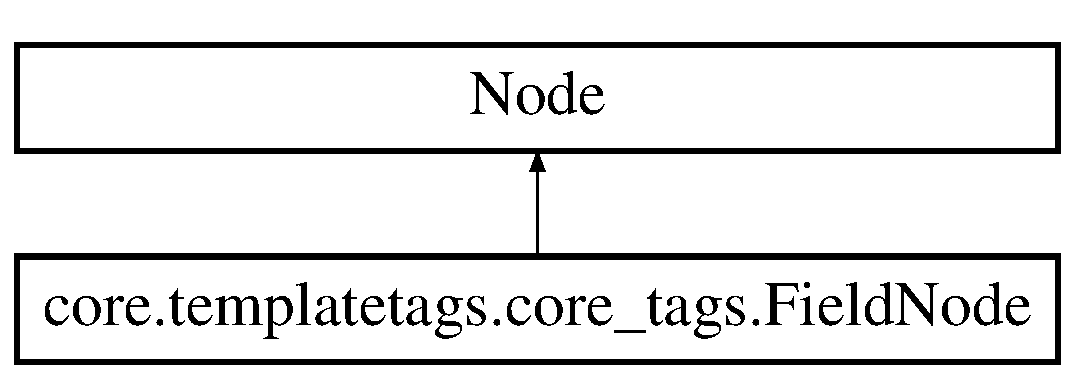
\includegraphics[height=2.000000cm]{classcore_1_1templatetags_1_1core__tags_1_1FieldNode}
\end{center}
\end{figure}
\subsection*{Public Member Functions}
\begin{DoxyCompactItemize}
\item 
def \hyperlink{classcore_1_1templatetags_1_1core__tags_1_1FieldNode_accb84d2afd89f30abe0e6916084e6b41}{\-\_\-\-\_\-init\-\_\-\-\_\-}
\item 
def \hyperlink{classcore_1_1templatetags_1_1core__tags_1_1FieldNode_ad1759f96de621b72fd8295f02b36ffe7}{render}
\end{DoxyCompactItemize}
\subsection*{Public Attributes}
\begin{DoxyCompactItemize}
\item 
\hyperlink{classcore_1_1templatetags_1_1core__tags_1_1FieldNode_a9d062381a044b5570b7e275e0ec7bc20}{field\-\_\-name}
\item 
\hyperlink{classcore_1_1templatetags_1_1core__tags_1_1FieldNode_ae7faeeff3066a619a964e5b34dbe398a}{field\-\_\-list}
\item 
\hyperlink{classcore_1_1templatetags_1_1core__tags_1_1FieldNode_aaf42c14788451f7dbe4a0cb92c4ddcb3}{field\-\_\-var}
\item 
\hyperlink{classcore_1_1templatetags_1_1core__tags_1_1FieldNode_a3d16b5fe648ccbdb38844010df869091}{instance}
\item 
\hyperlink{classcore_1_1templatetags_1_1core__tags_1_1FieldNode_aa5091f4c8032080baf130279fdcdf63d}{model}
\item 
\hyperlink{classcore_1_1templatetags_1_1core__tags_1_1FieldNode_a7e8856dc5073834638532b0fb9bc7971}{nodelist\-\_\-field}
\end{DoxyCompactItemize}


\subsection{Constructor \& Destructor Documentation}
\hypertarget{classcore_1_1templatetags_1_1core__tags_1_1FieldNode_accb84d2afd89f30abe0e6916084e6b41}{\index{core\-::templatetags\-::core\-\_\-tags\-::\-Field\-Node@{core\-::templatetags\-::core\-\_\-tags\-::\-Field\-Node}!\-\_\-\-\_\-init\-\_\-\-\_\-@{\-\_\-\-\_\-init\-\_\-\-\_\-}}
\index{\-\_\-\-\_\-init\-\_\-\-\_\-@{\-\_\-\-\_\-init\-\_\-\-\_\-}!core::templatetags::core_tags::FieldNode@{core\-::templatetags\-::core\-\_\-tags\-::\-Field\-Node}}
\subsubsection[{\-\_\-\-\_\-init\-\_\-\-\_\-}]{\setlength{\rightskip}{0pt plus 5cm}def core.\-templatetags.\-core\-\_\-tags.\-Field\-Node.\-\_\-\-\_\-init\-\_\-\-\_\- (
\begin{DoxyParamCaption}
\item[{}]{self, }
\item[{}]{field\-\_\-name, }
\item[{}]{field\-\_\-list, }
\item[{}]{field\-\_\-var, }
\item[{}]{instance, }
\item[{}]{model, }
\item[{}]{nodelist\-\_\-field}
\end{DoxyParamCaption}
)}}\label{classcore_1_1templatetags_1_1core__tags_1_1FieldNode_accb84d2afd89f30abe0e6916084e6b41}


\subsection{Member Function Documentation}
\hypertarget{classcore_1_1templatetags_1_1core__tags_1_1FieldNode_ad1759f96de621b72fd8295f02b36ffe7}{\index{core\-::templatetags\-::core\-\_\-tags\-::\-Field\-Node@{core\-::templatetags\-::core\-\_\-tags\-::\-Field\-Node}!render@{render}}
\index{render@{render}!core::templatetags::core_tags::FieldNode@{core\-::templatetags\-::core\-\_\-tags\-::\-Field\-Node}}
\subsubsection[{render}]{\setlength{\rightskip}{0pt plus 5cm}def core.\-templatetags.\-core\-\_\-tags.\-Field\-Node.\-render (
\begin{DoxyParamCaption}
\item[{}]{self, }
\item[{}]{context}
\end{DoxyParamCaption}
)}}\label{classcore_1_1templatetags_1_1core__tags_1_1FieldNode_ad1759f96de621b72fd8295f02b36ffe7}


\subsection{Member Data Documentation}
\hypertarget{classcore_1_1templatetags_1_1core__tags_1_1FieldNode_ae7faeeff3066a619a964e5b34dbe398a}{\index{core\-::templatetags\-::core\-\_\-tags\-::\-Field\-Node@{core\-::templatetags\-::core\-\_\-tags\-::\-Field\-Node}!field\-\_\-list@{field\-\_\-list}}
\index{field\-\_\-list@{field\-\_\-list}!core::templatetags::core_tags::FieldNode@{core\-::templatetags\-::core\-\_\-tags\-::\-Field\-Node}}
\subsubsection[{field\-\_\-list}]{\setlength{\rightskip}{0pt plus 5cm}core.\-templatetags.\-core\-\_\-tags.\-Field\-Node.\-field\-\_\-list}}\label{classcore_1_1templatetags_1_1core__tags_1_1FieldNode_ae7faeeff3066a619a964e5b34dbe398a}
\hypertarget{classcore_1_1templatetags_1_1core__tags_1_1FieldNode_a9d062381a044b5570b7e275e0ec7bc20}{\index{core\-::templatetags\-::core\-\_\-tags\-::\-Field\-Node@{core\-::templatetags\-::core\-\_\-tags\-::\-Field\-Node}!field\-\_\-name@{field\-\_\-name}}
\index{field\-\_\-name@{field\-\_\-name}!core::templatetags::core_tags::FieldNode@{core\-::templatetags\-::core\-\_\-tags\-::\-Field\-Node}}
\subsubsection[{field\-\_\-name}]{\setlength{\rightskip}{0pt plus 5cm}core.\-templatetags.\-core\-\_\-tags.\-Field\-Node.\-field\-\_\-name}}\label{classcore_1_1templatetags_1_1core__tags_1_1FieldNode_a9d062381a044b5570b7e275e0ec7bc20}
\hypertarget{classcore_1_1templatetags_1_1core__tags_1_1FieldNode_aaf42c14788451f7dbe4a0cb92c4ddcb3}{\index{core\-::templatetags\-::core\-\_\-tags\-::\-Field\-Node@{core\-::templatetags\-::core\-\_\-tags\-::\-Field\-Node}!field\-\_\-var@{field\-\_\-var}}
\index{field\-\_\-var@{field\-\_\-var}!core::templatetags::core_tags::FieldNode@{core\-::templatetags\-::core\-\_\-tags\-::\-Field\-Node}}
\subsubsection[{field\-\_\-var}]{\setlength{\rightskip}{0pt plus 5cm}core.\-templatetags.\-core\-\_\-tags.\-Field\-Node.\-field\-\_\-var}}\label{classcore_1_1templatetags_1_1core__tags_1_1FieldNode_aaf42c14788451f7dbe4a0cb92c4ddcb3}
\hypertarget{classcore_1_1templatetags_1_1core__tags_1_1FieldNode_a3d16b5fe648ccbdb38844010df869091}{\index{core\-::templatetags\-::core\-\_\-tags\-::\-Field\-Node@{core\-::templatetags\-::core\-\_\-tags\-::\-Field\-Node}!instance@{instance}}
\index{instance@{instance}!core::templatetags::core_tags::FieldNode@{core\-::templatetags\-::core\-\_\-tags\-::\-Field\-Node}}
\subsubsection[{instance}]{\setlength{\rightskip}{0pt plus 5cm}core.\-templatetags.\-core\-\_\-tags.\-Field\-Node.\-instance}}\label{classcore_1_1templatetags_1_1core__tags_1_1FieldNode_a3d16b5fe648ccbdb38844010df869091}
\hypertarget{classcore_1_1templatetags_1_1core__tags_1_1FieldNode_aa5091f4c8032080baf130279fdcdf63d}{\index{core\-::templatetags\-::core\-\_\-tags\-::\-Field\-Node@{core\-::templatetags\-::core\-\_\-tags\-::\-Field\-Node}!model@{model}}
\index{model@{model}!core::templatetags::core_tags::FieldNode@{core\-::templatetags\-::core\-\_\-tags\-::\-Field\-Node}}
\subsubsection[{model}]{\setlength{\rightskip}{0pt plus 5cm}core.\-templatetags.\-core\-\_\-tags.\-Field\-Node.\-model}}\label{classcore_1_1templatetags_1_1core__tags_1_1FieldNode_aa5091f4c8032080baf130279fdcdf63d}
\hypertarget{classcore_1_1templatetags_1_1core__tags_1_1FieldNode_a7e8856dc5073834638532b0fb9bc7971}{\index{core\-::templatetags\-::core\-\_\-tags\-::\-Field\-Node@{core\-::templatetags\-::core\-\_\-tags\-::\-Field\-Node}!nodelist\-\_\-field@{nodelist\-\_\-field}}
\index{nodelist\-\_\-field@{nodelist\-\_\-field}!core::templatetags::core_tags::FieldNode@{core\-::templatetags\-::core\-\_\-tags\-::\-Field\-Node}}
\subsubsection[{nodelist\-\_\-field}]{\setlength{\rightskip}{0pt plus 5cm}core.\-templatetags.\-core\-\_\-tags.\-Field\-Node.\-nodelist\-\_\-field}}\label{classcore_1_1templatetags_1_1core__tags_1_1FieldNode_a7e8856dc5073834638532b0fb9bc7971}


The documentation for this class was generated from the following file\-:\begin{DoxyCompactItemize}
\item 
/wepo/core/templatetags/\hyperlink{core__tags_8py}{core\-\_\-tags.\-py}\end{DoxyCompactItemize}

\hypertarget{classcore_1_1models_1_1File}{\section{core.\-models.\-File Class Reference}
\label{classcore_1_1models_1_1File}\index{core.\-models.\-File@{core.\-models.\-File}}
}


\hyperlink{classcore_1_1models_1_1File}{File}.  


Inheritance diagram for core.\-models.\-File\-:\begin{figure}[H]
\begin{center}
\leavevmode
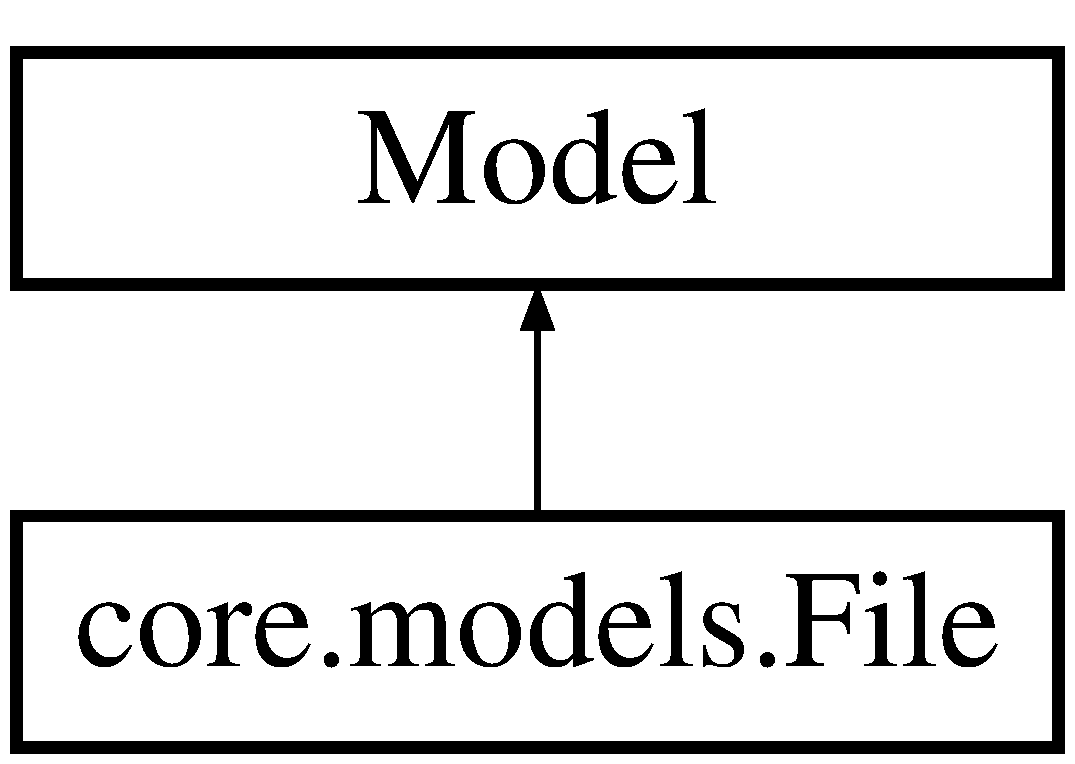
\includegraphics[height=2.000000cm]{classcore_1_1models_1_1File}
\end{center}
\end{figure}
\subsection*{Classes}
\begin{DoxyCompactItemize}
\item 
class \hyperlink{classcore_1_1models_1_1File_1_1Meta}{Meta}
\end{DoxyCompactItemize}
\subsection*{Public Member Functions}
\begin{DoxyCompactItemize}
\item 
def \hyperlink{classcore_1_1models_1_1File_aa55a62aec4d1cbfab35d6a3acbcb7839}{\-\_\-\-\_\-unicode\-\_\-\-\_\-}
\item 
def \hyperlink{classcore_1_1models_1_1File_a22cd87afedaecdd3f0106d14f537602e}{save}
\begin{DoxyCompactList}\small\item\em Custom save method. \end{DoxyCompactList}\item 
def \hyperlink{classcore_1_1models_1_1File_a8b5338739bfbf9271fbe914ff6024d77}{get\-\_\-seo}
\begin{DoxyCompactList}\small\item\em Get seo link. \end{DoxyCompactList}\end{DoxyCompactItemize}
\subsection*{Static Public Attributes}
\begin{DoxyCompactItemize}
\item 
tuple \hyperlink{classcore_1_1models_1_1File_a00e09db629f9ff8114662c4e950927bb}{file\-\_\-name} = dmodels.\-Char\-Field(max\-\_\-length=255, db\-\_\-index=True)
\begin{DoxyCompactList}\small\item\em \hyperlink{classcore_1_1models_1_1File}{File} name of the file. \end{DoxyCompactList}\item 
tuple \hyperlink{classcore_1_1models_1_1File_aedfac4d90aea7deacffb837534bb92bc}{mime\-\_\-type} = dmodels.\-Char\-Field(max\-\_\-length=255, db\-\_\-index=True)
\begin{DoxyCompactList}\small\item\em Unique identifier of the file. \end{DoxyCompactList}\item 
tuple \hyperlink{classcore_1_1models_1_1File_a18f6917981a73daa38b337f1e167c2d5}{size} = dmodels.\-Char\-Field(max\-\_\-length=255)
\begin{DoxyCompactList}\small\item\em \hyperlink{classcore_1_1models_1_1File}{File} size. \end{DoxyCompactList}\item 
tuple \hyperlink{classcore_1_1models_1_1File_a8b5744511785ff36e1312245bb92955e}{title} = dmodels.\-Text\-Field()
\begin{DoxyCompactList}\small\item\em Title of the file. \end{DoxyCompactList}\item 
tuple \hyperlink{classcore_1_1models_1_1File_a3ba747aa055c9952345d32fd0a2e93df}{description} = dmodels.\-Text\-Field()
\begin{DoxyCompactList}\small\item\em Description of the file. \end{DoxyCompactList}\item 
tuple \hyperlink{classcore_1_1models_1_1File_a4b56e6ce2f5bd75ad78f41cea297fd49}{author} = dmodels.\-Text\-Field()
\begin{DoxyCompactList}\small\item\em Author of the file. \end{DoxyCompactList}\item 
tuple \hyperlink{classcore_1_1models_1_1File_a5e8a1bacede61e2e1f2386907e63e274}{path} = dmodels.\-Text\-Field()
\begin{DoxyCompactList}\small\item\em \hyperlink{classcore_1_1models_1_1File}{File} path. \end{DoxyCompactList}\item 
tuple \hyperlink{classcore_1_1models_1_1File_a786c3b3f61bd0e38ea5d32310391a235}{data} = \hyperlink{classcore_1_1fields_1_1JsonField}{Json\-Field}(null=True, blank=True)
\begin{DoxyCompactList}\small\item\em Data about crops, different sizes, etc... \end{DoxyCompactList}\item 
tuple \hyperlink{classcore_1_1models_1_1File_adaa3cc04ed44b20d1796df296373e9ba}{created} = dmodels.\-Date\-Time\-Field(db\-\_\-index=True)
\begin{DoxyCompactList}\small\item\em Date time of creation. \end{DoxyCompactList}\item 
tuple \hyperlink{classcore_1_1models_1_1File_a65e05c5c5dee44c2c73d8a202845209f}{directory} = dmodels.\-Foreign\-Key('\hyperlink{classcore_1_1models_1_1Directory}{Directory}', null=True, blank=True)
\begin{DoxyCompactList}\small\item\em Virtual directory. \end{DoxyCompactList}\item 
tuple \hyperlink{classcore_1_1models_1_1File_a1925fe1551da140f13cb0295d3c250a3}{owner} = dmodels.\-Foreign\-Key('\hyperlink{classcore_1_1models_1_1User}{User}', null=True, blank=True)
\begin{DoxyCompactList}\small\item\em \hyperlink{classcore_1_1models_1_1File}{File} owner (uploader) \end{DoxyCompactList}\end{DoxyCompactItemize}


\subsection{Detailed Description}
\hyperlink{classcore_1_1models_1_1File}{File}. 

Files 

\subsection{Member Function Documentation}
\hypertarget{classcore_1_1models_1_1File_aa55a62aec4d1cbfab35d6a3acbcb7839}{\index{core\-::models\-::\-File@{core\-::models\-::\-File}!\-\_\-\-\_\-unicode\-\_\-\-\_\-@{\-\_\-\-\_\-unicode\-\_\-\-\_\-}}
\index{\-\_\-\-\_\-unicode\-\_\-\-\_\-@{\-\_\-\-\_\-unicode\-\_\-\-\_\-}!core::models::File@{core\-::models\-::\-File}}
\subsubsection[{\-\_\-\-\_\-unicode\-\_\-\-\_\-}]{\setlength{\rightskip}{0pt plus 5cm}def core.\-models.\-File.\-\_\-\-\_\-unicode\-\_\-\-\_\- (
\begin{DoxyParamCaption}
\item[{}]{self}
\end{DoxyParamCaption}
)}}\label{classcore_1_1models_1_1File_aa55a62aec4d1cbfab35d6a3acbcb7839}
\hypertarget{classcore_1_1models_1_1File_a8b5338739bfbf9271fbe914ff6024d77}{\index{core\-::models\-::\-File@{core\-::models\-::\-File}!get\-\_\-seo@{get\-\_\-seo}}
\index{get\-\_\-seo@{get\-\_\-seo}!core::models::File@{core\-::models\-::\-File}}
\subsubsection[{get\-\_\-seo}]{\setlength{\rightskip}{0pt plus 5cm}def core.\-models.\-File.\-get\-\_\-seo (
\begin{DoxyParamCaption}
\item[{}]{self}
\end{DoxyParamCaption}
)}}\label{classcore_1_1models_1_1File_a8b5338739bfbf9271fbe914ff6024d77}


Get seo link. 

\hypertarget{classcore_1_1models_1_1File_a22cd87afedaecdd3f0106d14f537602e}{\index{core\-::models\-::\-File@{core\-::models\-::\-File}!save@{save}}
\index{save@{save}!core::models::File@{core\-::models\-::\-File}}
\subsubsection[{save}]{\setlength{\rightskip}{0pt plus 5cm}def core.\-models.\-File.\-save (
\begin{DoxyParamCaption}
\item[{}]{self, }
\item[{}]{force\-\_\-insert = {\ttfamily False}, }
\item[{}]{force\-\_\-update = {\ttfamily False}, }
\item[{}]{using = {\ttfamily None}, }
\item[{}]{update\-\_\-fields = {\ttfamily None}}
\end{DoxyParamCaption}
)}}\label{classcore_1_1models_1_1File_a22cd87afedaecdd3f0106d14f537602e}


Custom save method. 



\subsection{Member Data Documentation}
\hypertarget{classcore_1_1models_1_1File_a4b56e6ce2f5bd75ad78f41cea297fd49}{\index{core\-::models\-::\-File@{core\-::models\-::\-File}!author@{author}}
\index{author@{author}!core::models::File@{core\-::models\-::\-File}}
\subsubsection[{author}]{\setlength{\rightskip}{0pt plus 5cm}core.\-models.\-File.\-author = dmodels.\-Text\-Field()\hspace{0.3cm}{\ttfamily [static]}}}\label{classcore_1_1models_1_1File_a4b56e6ce2f5bd75ad78f41cea297fd49}


Author of the file. 

\hypertarget{classcore_1_1models_1_1File_adaa3cc04ed44b20d1796df296373e9ba}{\index{core\-::models\-::\-File@{core\-::models\-::\-File}!created@{created}}
\index{created@{created}!core::models::File@{core\-::models\-::\-File}}
\subsubsection[{created}]{\setlength{\rightskip}{0pt plus 5cm}core.\-models.\-File.\-created = dmodels.\-Date\-Time\-Field(db\-\_\-index=True)\hspace{0.3cm}{\ttfamily [static]}}}\label{classcore_1_1models_1_1File_adaa3cc04ed44b20d1796df296373e9ba}


Date time of creation. 

\hypertarget{classcore_1_1models_1_1File_a786c3b3f61bd0e38ea5d32310391a235}{\index{core\-::models\-::\-File@{core\-::models\-::\-File}!data@{data}}
\index{data@{data}!core::models::File@{core\-::models\-::\-File}}
\subsubsection[{data}]{\setlength{\rightskip}{0pt plus 5cm}core.\-models.\-File.\-data = {\bf Json\-Field}(null=True, blank=True)\hspace{0.3cm}{\ttfamily [static]}}}\label{classcore_1_1models_1_1File_a786c3b3f61bd0e38ea5d32310391a235}


Data about crops, different sizes, etc... 

\hypertarget{classcore_1_1models_1_1File_a3ba747aa055c9952345d32fd0a2e93df}{\index{core\-::models\-::\-File@{core\-::models\-::\-File}!description@{description}}
\index{description@{description}!core::models::File@{core\-::models\-::\-File}}
\subsubsection[{description}]{\setlength{\rightskip}{0pt plus 5cm}core.\-models.\-File.\-description = dmodels.\-Text\-Field()\hspace{0.3cm}{\ttfamily [static]}}}\label{classcore_1_1models_1_1File_a3ba747aa055c9952345d32fd0a2e93df}


Description of the file. 

\hypertarget{classcore_1_1models_1_1File_a65e05c5c5dee44c2c73d8a202845209f}{\index{core\-::models\-::\-File@{core\-::models\-::\-File}!directory@{directory}}
\index{directory@{directory}!core::models::File@{core\-::models\-::\-File}}
\subsubsection[{directory}]{\setlength{\rightskip}{0pt plus 5cm}core.\-models.\-File.\-directory = dmodels.\-Foreign\-Key('{\bf Directory}', null=True, blank=True)\hspace{0.3cm}{\ttfamily [static]}}}\label{classcore_1_1models_1_1File_a65e05c5c5dee44c2c73d8a202845209f}


Virtual directory. 

\hypertarget{classcore_1_1models_1_1File_a00e09db629f9ff8114662c4e950927bb}{\index{core\-::models\-::\-File@{core\-::models\-::\-File}!file\-\_\-name@{file\-\_\-name}}
\index{file\-\_\-name@{file\-\_\-name}!core::models::File@{core\-::models\-::\-File}}
\subsubsection[{file\-\_\-name}]{\setlength{\rightskip}{0pt plus 5cm}core.\-models.\-File.\-file\-\_\-name = dmodels.\-Char\-Field(max\-\_\-length=255, db\-\_\-index=True)\hspace{0.3cm}{\ttfamily [static]}}}\label{classcore_1_1models_1_1File_a00e09db629f9ff8114662c4e950927bb}


\hyperlink{classcore_1_1models_1_1File}{File} name of the file. 

\hypertarget{classcore_1_1models_1_1File_aedfac4d90aea7deacffb837534bb92bc}{\index{core\-::models\-::\-File@{core\-::models\-::\-File}!mime\-\_\-type@{mime\-\_\-type}}
\index{mime\-\_\-type@{mime\-\_\-type}!core::models::File@{core\-::models\-::\-File}}
\subsubsection[{mime\-\_\-type}]{\setlength{\rightskip}{0pt plus 5cm}core.\-models.\-File.\-mime\-\_\-type = dmodels.\-Char\-Field(max\-\_\-length=255, db\-\_\-index=True)\hspace{0.3cm}{\ttfamily [static]}}}\label{classcore_1_1models_1_1File_aedfac4d90aea7deacffb837534bb92bc}


Unique identifier of the file. 

\hypertarget{classcore_1_1models_1_1File_a1925fe1551da140f13cb0295d3c250a3}{\index{core\-::models\-::\-File@{core\-::models\-::\-File}!owner@{owner}}
\index{owner@{owner}!core::models::File@{core\-::models\-::\-File}}
\subsubsection[{owner}]{\setlength{\rightskip}{0pt plus 5cm}core.\-models.\-File.\-owner = dmodels.\-Foreign\-Key('{\bf User}', null=True, blank=True)\hspace{0.3cm}{\ttfamily [static]}}}\label{classcore_1_1models_1_1File_a1925fe1551da140f13cb0295d3c250a3}


\hyperlink{classcore_1_1models_1_1File}{File} owner (uploader) 

\hypertarget{classcore_1_1models_1_1File_a5e8a1bacede61e2e1f2386907e63e274}{\index{core\-::models\-::\-File@{core\-::models\-::\-File}!path@{path}}
\index{path@{path}!core::models::File@{core\-::models\-::\-File}}
\subsubsection[{path}]{\setlength{\rightskip}{0pt plus 5cm}core.\-models.\-File.\-path = dmodels.\-Text\-Field()\hspace{0.3cm}{\ttfamily [static]}}}\label{classcore_1_1models_1_1File_a5e8a1bacede61e2e1f2386907e63e274}


\hyperlink{classcore_1_1models_1_1File}{File} path. 

\hypertarget{classcore_1_1models_1_1File_a18f6917981a73daa38b337f1e167c2d5}{\index{core\-::models\-::\-File@{core\-::models\-::\-File}!size@{size}}
\index{size@{size}!core::models::File@{core\-::models\-::\-File}}
\subsubsection[{size}]{\setlength{\rightskip}{0pt plus 5cm}core.\-models.\-File.\-size = dmodels.\-Char\-Field(max\-\_\-length=255)\hspace{0.3cm}{\ttfamily [static]}}}\label{classcore_1_1models_1_1File_a18f6917981a73daa38b337f1e167c2d5}


\hyperlink{classcore_1_1models_1_1File}{File} size. 

\hypertarget{classcore_1_1models_1_1File_a8b5744511785ff36e1312245bb92955e}{\index{core\-::models\-::\-File@{core\-::models\-::\-File}!title@{title}}
\index{title@{title}!core::models::File@{core\-::models\-::\-File}}
\subsubsection[{title}]{\setlength{\rightskip}{0pt plus 5cm}core.\-models.\-File.\-title = dmodels.\-Text\-Field()\hspace{0.3cm}{\ttfamily [static]}}}\label{classcore_1_1models_1_1File_a8b5744511785ff36e1312245bb92955e}


Title of the file. 



The documentation for this class was generated from the following file\-:\begin{DoxyCompactItemize}
\item 
/wepo/core/\hyperlink{models_8py}{models.\-py}\end{DoxyCompactItemize}

\hypertarget{classcore_1_1form_1_1Form}{\section{core.\-form.\-Form Class Reference}
\label{classcore_1_1form_1_1Form}\index{core.\-form.\-Form@{core.\-form.\-Form}}
}


Wepo form class.  


\subsection*{Public Member Functions}
\begin{DoxyCompactItemize}
\item 
def \hyperlink{classcore_1_1form_1_1Form_a8ffb534c4eb20f7ff59e98f3f78950da}{\-\_\-\-\_\-init\-\_\-\-\_\-}
\begin{DoxyCompactList}\small\item\em \hyperlink{classcore_1_1form_1_1Form}{Form} constructor. \end{DoxyCompactList}\item 
def \hyperlink{classcore_1_1form_1_1Form_a20903823a9d10f7f5731a297a43e5174}{add\-\_\-item}
\begin{DoxyCompactList}\small\item\em Add new item to the form. \end{DoxyCompactList}\item 
def \hyperlink{classcore_1_1form_1_1Form_a42834e70bfd5e0d3234e444aeb9f1e2b}{remove\-\_\-item}
\begin{DoxyCompactList}\small\item\em Remove item from the form. \end{DoxyCompactList}\item 
def \hyperlink{classcore_1_1form_1_1Form_aa1e30c2929cb20f7a99707f2cf877f1f}{add\-\_\-group}
\begin{DoxyCompactList}\small\item\em Add new item to the form. \end{DoxyCompactList}\item 
def \hyperlink{classcore_1_1form_1_1Form_a082e72f90f3ac0e4388a8447c13b1160}{render}
\begin{DoxyCompactList}\small\item\em Render form. \end{DoxyCompactList}\item 
def \hyperlink{classcore_1_1form_1_1Form_ab35349daa612e98cb9c85717cde28e4f}{\-\_\-\-\_\-str\-\_\-\-\_\-}
\begin{DoxyCompactList}\small\item\em Render in template. \end{DoxyCompactList}\item 
def \hyperlink{classcore_1_1form_1_1Form_a5dbfa902ee08b5793b8855b80775a7a5}{\-\_\-\-\_\-iter\-\_\-\-\_\-}
\begin{DoxyCompactList}\small\item\em Iterate trough items. \end{DoxyCompactList}\end{DoxyCompactItemize}
\subsection*{Public Attributes}
\begin{DoxyCompactItemize}
\item 
\hyperlink{classcore_1_1form_1_1Form_a1a92a929b21b377272e0370f23474bd5}{items}
\item 
\hyperlink{classcore_1_1form_1_1Form_a1a7dc338f5bd83c47e9e9750d9dc452e}{action}
\item 
\hyperlink{classcore_1_1form_1_1Form_af4551d0a9109ae655e567dea1263fdc8}{name}
\item 
\hyperlink{classcore_1_1form_1_1Form_adefa2bf3828a790476c15912de2d0c80}{method}
\item 
\hyperlink{classcore_1_1form_1_1Form_a0046020aebc28839db2ccb6c354700c0}{request}
\item 
\hyperlink{classcore_1_1form_1_1Form_aab448845667090194d33e51c395fd7e5}{attributes}
\end{DoxyCompactItemize}


\subsection{Detailed Description}
Wepo form class. 

\subsection{Constructor \& Destructor Documentation}
\hypertarget{classcore_1_1form_1_1Form_a8ffb534c4eb20f7ff59e98f3f78950da}{\index{core\-::form\-::\-Form@{core\-::form\-::\-Form}!\-\_\-\-\_\-init\-\_\-\-\_\-@{\-\_\-\-\_\-init\-\_\-\-\_\-}}
\index{\-\_\-\-\_\-init\-\_\-\-\_\-@{\-\_\-\-\_\-init\-\_\-\-\_\-}!core::form::Form@{core\-::form\-::\-Form}}
\subsubsection[{\-\_\-\-\_\-init\-\_\-\-\_\-}]{\setlength{\rightskip}{0pt plus 5cm}def core.\-form.\-Form.\-\_\-\-\_\-init\-\_\-\-\_\- (
\begin{DoxyParamCaption}
\item[{}]{self, }
\item[{}]{request, }
\item[{}]{action = {\ttfamily None}, }
\item[{}]{name = {\ttfamily None}, }
\item[{}]{method = {\ttfamily None}, }
\item[{}]{attributes}
\end{DoxyParamCaption}
)}}\label{classcore_1_1form_1_1Form_a8ffb534c4eb20f7ff59e98f3f78950da}


\hyperlink{classcore_1_1form_1_1Form}{Form} constructor. 


\begin{DoxyParams}{Parameters}
{\em request} & Current request \\
\hline
{\em action} & \hyperlink{classcore_1_1form_1_1Form}{Form} action \\
\hline
{\em name} & \hyperlink{classcore_1_1form_1_1Form}{Form} name \\
\hline
{\em method} & \hyperlink{classcore_1_1form_1_1Form}{Form} method \\
\hline
{\em attributes} & Extra form attributes \\
\hline
\end{DoxyParams}


\subsection{Member Function Documentation}
\hypertarget{classcore_1_1form_1_1Form_a5dbfa902ee08b5793b8855b80775a7a5}{\index{core\-::form\-::\-Form@{core\-::form\-::\-Form}!\-\_\-\-\_\-iter\-\_\-\-\_\-@{\-\_\-\-\_\-iter\-\_\-\-\_\-}}
\index{\-\_\-\-\_\-iter\-\_\-\-\_\-@{\-\_\-\-\_\-iter\-\_\-\-\_\-}!core::form::Form@{core\-::form\-::\-Form}}
\subsubsection[{\-\_\-\-\_\-iter\-\_\-\-\_\-}]{\setlength{\rightskip}{0pt plus 5cm}def core.\-form.\-Form.\-\_\-\-\_\-iter\-\_\-\-\_\- (
\begin{DoxyParamCaption}
\item[{}]{self}
\end{DoxyParamCaption}
)}}\label{classcore_1_1form_1_1Form_a5dbfa902ee08b5793b8855b80775a7a5}


Iterate trough items. 

\hypertarget{classcore_1_1form_1_1Form_ab35349daa612e98cb9c85717cde28e4f}{\index{core\-::form\-::\-Form@{core\-::form\-::\-Form}!\-\_\-\-\_\-str\-\_\-\-\_\-@{\-\_\-\-\_\-str\-\_\-\-\_\-}}
\index{\-\_\-\-\_\-str\-\_\-\-\_\-@{\-\_\-\-\_\-str\-\_\-\-\_\-}!core::form::Form@{core\-::form\-::\-Form}}
\subsubsection[{\-\_\-\-\_\-str\-\_\-\-\_\-}]{\setlength{\rightskip}{0pt plus 5cm}def core.\-form.\-Form.\-\_\-\-\_\-str\-\_\-\-\_\- (
\begin{DoxyParamCaption}
\item[{}]{self}
\end{DoxyParamCaption}
)}}\label{classcore_1_1form_1_1Form_ab35349daa612e98cb9c85717cde28e4f}


Render in template. 

\hypertarget{classcore_1_1form_1_1Form_aa1e30c2929cb20f7a99707f2cf877f1f}{\index{core\-::form\-::\-Form@{core\-::form\-::\-Form}!add\-\_\-group@{add\-\_\-group}}
\index{add\-\_\-group@{add\-\_\-group}!core::form::Form@{core\-::form\-::\-Form}}
\subsubsection[{add\-\_\-group}]{\setlength{\rightskip}{0pt plus 5cm}def core.\-form.\-Form.\-add\-\_\-group (
\begin{DoxyParamCaption}
\item[{}]{self, }
\item[{}]{attributes}
\end{DoxyParamCaption}
)}}\label{classcore_1_1form_1_1Form_aa1e30c2929cb20f7a99707f2cf877f1f}


Add new item to the form. 


\begin{DoxyParams}{Parameters}
{\em request} & Current request \\
\hline
{\em attributes} & Extra form attributes\\
\hline
\end{DoxyParams}
\begin{DoxyReturn}{Returns}
Create group 
\end{DoxyReturn}
\hypertarget{classcore_1_1form_1_1Form_a20903823a9d10f7f5731a297a43e5174}{\index{core\-::form\-::\-Form@{core\-::form\-::\-Form}!add\-\_\-item@{add\-\_\-item}}
\index{add\-\_\-item@{add\-\_\-item}!core::form::Form@{core\-::form\-::\-Form}}
\subsubsection[{add\-\_\-item}]{\setlength{\rightskip}{0pt plus 5cm}def core.\-form.\-Form.\-add\-\_\-item (
\begin{DoxyParamCaption}
\item[{}]{self, }
\item[{}]{type, }
\item[{}]{attributes}
\end{DoxyParamCaption}
)}}\label{classcore_1_1form_1_1Form_a20903823a9d10f7f5731a297a43e5174}


Add new item to the form. 


\begin{DoxyParams}{Parameters}
{\em type} & \hyperlink{classcore_1_1form_1_1Form}{Form} item type \\
\hline
{\em request} & Current request \\
\hline
{\em attributes} & Extra form attributes\\
\hline
\end{DoxyParams}
\begin{DoxyReturn}{Returns}
Create item 
\end{DoxyReturn}
\hypertarget{classcore_1_1form_1_1Form_a42834e70bfd5e0d3234e444aeb9f1e2b}{\index{core\-::form\-::\-Form@{core\-::form\-::\-Form}!remove\-\_\-item@{remove\-\_\-item}}
\index{remove\-\_\-item@{remove\-\_\-item}!core::form::Form@{core\-::form\-::\-Form}}
\subsubsection[{remove\-\_\-item}]{\setlength{\rightskip}{0pt plus 5cm}def core.\-form.\-Form.\-remove\-\_\-item (
\begin{DoxyParamCaption}
\item[{}]{self, }
\item[{}]{index}
\end{DoxyParamCaption}
)}}\label{classcore_1_1form_1_1Form_a42834e70bfd5e0d3234e444aeb9f1e2b}


Remove item from the form. 


\begin{DoxyParams}{Parameters}
{\em index} & Index of the item to be removed \\
\hline
\end{DoxyParams}
\hypertarget{classcore_1_1form_1_1Form_a082e72f90f3ac0e4388a8447c13b1160}{\index{core\-::form\-::\-Form@{core\-::form\-::\-Form}!render@{render}}
\index{render@{render}!core::form::Form@{core\-::form\-::\-Form}}
\subsubsection[{render}]{\setlength{\rightskip}{0pt plus 5cm}def core.\-form.\-Form.\-render (
\begin{DoxyParamCaption}
\item[{}]{self}
\end{DoxyParamCaption}
)}}\label{classcore_1_1form_1_1Form_a082e72f90f3ac0e4388a8447c13b1160}


Render form. 

\begin{DoxyReturn}{Returns}
Rendered form 
\end{DoxyReturn}


\subsection{Member Data Documentation}
\hypertarget{classcore_1_1form_1_1Form_a1a7dc338f5bd83c47e9e9750d9dc452e}{\index{core\-::form\-::\-Form@{core\-::form\-::\-Form}!action@{action}}
\index{action@{action}!core::form::Form@{core\-::form\-::\-Form}}
\subsubsection[{action}]{\setlength{\rightskip}{0pt plus 5cm}core.\-form.\-Form.\-action}}\label{classcore_1_1form_1_1Form_a1a7dc338f5bd83c47e9e9750d9dc452e}
\hypertarget{classcore_1_1form_1_1Form_aab448845667090194d33e51c395fd7e5}{\index{core\-::form\-::\-Form@{core\-::form\-::\-Form}!attributes@{attributes}}
\index{attributes@{attributes}!core::form::Form@{core\-::form\-::\-Form}}
\subsubsection[{attributes}]{\setlength{\rightskip}{0pt plus 5cm}core.\-form.\-Form.\-attributes}}\label{classcore_1_1form_1_1Form_aab448845667090194d33e51c395fd7e5}
\hypertarget{classcore_1_1form_1_1Form_a1a92a929b21b377272e0370f23474bd5}{\index{core\-::form\-::\-Form@{core\-::form\-::\-Form}!items@{items}}
\index{items@{items}!core::form::Form@{core\-::form\-::\-Form}}
\subsubsection[{items}]{\setlength{\rightskip}{0pt plus 5cm}core.\-form.\-Form.\-items}}\label{classcore_1_1form_1_1Form_a1a92a929b21b377272e0370f23474bd5}
\hypertarget{classcore_1_1form_1_1Form_adefa2bf3828a790476c15912de2d0c80}{\index{core\-::form\-::\-Form@{core\-::form\-::\-Form}!method@{method}}
\index{method@{method}!core::form::Form@{core\-::form\-::\-Form}}
\subsubsection[{method}]{\setlength{\rightskip}{0pt plus 5cm}core.\-form.\-Form.\-method}}\label{classcore_1_1form_1_1Form_adefa2bf3828a790476c15912de2d0c80}
\hypertarget{classcore_1_1form_1_1Form_af4551d0a9109ae655e567dea1263fdc8}{\index{core\-::form\-::\-Form@{core\-::form\-::\-Form}!name@{name}}
\index{name@{name}!core::form::Form@{core\-::form\-::\-Form}}
\subsubsection[{name}]{\setlength{\rightskip}{0pt plus 5cm}core.\-form.\-Form.\-name}}\label{classcore_1_1form_1_1Form_af4551d0a9109ae655e567dea1263fdc8}
\hypertarget{classcore_1_1form_1_1Form_a0046020aebc28839db2ccb6c354700c0}{\index{core\-::form\-::\-Form@{core\-::form\-::\-Form}!request@{request}}
\index{request@{request}!core::form::Form@{core\-::form\-::\-Form}}
\subsubsection[{request}]{\setlength{\rightskip}{0pt plus 5cm}core.\-form.\-Form.\-request}}\label{classcore_1_1form_1_1Form_a0046020aebc28839db2ccb6c354700c0}


The documentation for this class was generated from the following file\-:\begin{DoxyCompactItemize}
\item 
/wepo/core/form/\hyperlink{core_2form_2____init_____8py}{\-\_\-\-\_\-init\-\_\-\-\_\-.\-py}\end{DoxyCompactItemize}

\hypertarget{classcore_1_1form_1_1FormGroup}{\section{core.\-form.\-Form\-Group Class Reference}
\label{classcore_1_1form_1_1FormGroup}\index{core.\-form.\-Form\-Group@{core.\-form.\-Form\-Group}}
}


Wepo form field sets class.  


\subsection*{Public Member Functions}
\begin{DoxyCompactItemize}
\item 
def \hyperlink{classcore_1_1form_1_1FormGroup_a89e8497987edca32795491ad1238aab8}{\-\_\-\-\_\-init\-\_\-\-\_\-}
\item 
def \hyperlink{classcore_1_1form_1_1FormGroup_a2601bc2dc15971645ed97c73af5bfc31}{add\-\_\-item}
\begin{DoxyCompactList}\small\item\em Add new item to the form. \end{DoxyCompactList}\item 
def \hyperlink{classcore_1_1form_1_1FormGroup_aaaee5425b1449922053ec97050e146bd}{remove\-\_\-item}
\begin{DoxyCompactList}\small\item\em Remove item from the form. \end{DoxyCompactList}\item 
def \hyperlink{classcore_1_1form_1_1FormGroup_ac341c438ac1772576b2ab7364f6b0702}{render}
\begin{DoxyCompactList}\small\item\em Render form group. \end{DoxyCompactList}\item 
def \hyperlink{classcore_1_1form_1_1FormGroup_a6a0f5cdacadba5a4ae75330852edbd5a}{\-\_\-\-\_\-iter\-\_\-\-\_\-}
\begin{DoxyCompactList}\small\item\em Iterate trough items. \end{DoxyCompactList}\end{DoxyCompactItemize}
\subsection*{Public Attributes}
\begin{DoxyCompactItemize}
\item 
\hyperlink{classcore_1_1form_1_1FormGroup_a322dc0daa2a6a01b88ac158cfd78619a}{items}
\item 
\hyperlink{classcore_1_1form_1_1FormGroup_acfa014f999bdb99af51a14f6754cff9f}{request}
\item 
\hyperlink{classcore_1_1form_1_1FormGroup_a7b682a9b4f5c15cf28f2c2d2d5a2d9ef}{attributes}
\end{DoxyCompactItemize}


\subsection{Detailed Description}
Wepo form field sets class. 

\subsection{Constructor \& Destructor Documentation}
\hypertarget{classcore_1_1form_1_1FormGroup_a89e8497987edca32795491ad1238aab8}{\index{core\-::form\-::\-Form\-Group@{core\-::form\-::\-Form\-Group}!\-\_\-\-\_\-init\-\_\-\-\_\-@{\-\_\-\-\_\-init\-\_\-\-\_\-}}
\index{\-\_\-\-\_\-init\-\_\-\-\_\-@{\-\_\-\-\_\-init\-\_\-\-\_\-}!core::form::FormGroup@{core\-::form\-::\-Form\-Group}}
\subsubsection[{\-\_\-\-\_\-init\-\_\-\-\_\-}]{\setlength{\rightskip}{0pt plus 5cm}def core.\-form.\-Form\-Group.\-\_\-\-\_\-init\-\_\-\-\_\- (
\begin{DoxyParamCaption}
\item[{}]{self, }
\item[{}]{request, }
\item[{}]{attributes}
\end{DoxyParamCaption}
)}}\label{classcore_1_1form_1_1FormGroup_a89e8497987edca32795491ad1238aab8}


\subsection{Member Function Documentation}
\hypertarget{classcore_1_1form_1_1FormGroup_a6a0f5cdacadba5a4ae75330852edbd5a}{\index{core\-::form\-::\-Form\-Group@{core\-::form\-::\-Form\-Group}!\-\_\-\-\_\-iter\-\_\-\-\_\-@{\-\_\-\-\_\-iter\-\_\-\-\_\-}}
\index{\-\_\-\-\_\-iter\-\_\-\-\_\-@{\-\_\-\-\_\-iter\-\_\-\-\_\-}!core::form::FormGroup@{core\-::form\-::\-Form\-Group}}
\subsubsection[{\-\_\-\-\_\-iter\-\_\-\-\_\-}]{\setlength{\rightskip}{0pt plus 5cm}def core.\-form.\-Form\-Group.\-\_\-\-\_\-iter\-\_\-\-\_\- (
\begin{DoxyParamCaption}
\item[{}]{self}
\end{DoxyParamCaption}
)}}\label{classcore_1_1form_1_1FormGroup_a6a0f5cdacadba5a4ae75330852edbd5a}


Iterate trough items. 

\hypertarget{classcore_1_1form_1_1FormGroup_a2601bc2dc15971645ed97c73af5bfc31}{\index{core\-::form\-::\-Form\-Group@{core\-::form\-::\-Form\-Group}!add\-\_\-item@{add\-\_\-item}}
\index{add\-\_\-item@{add\-\_\-item}!core::form::FormGroup@{core\-::form\-::\-Form\-Group}}
\subsubsection[{add\-\_\-item}]{\setlength{\rightskip}{0pt plus 5cm}def core.\-form.\-Form\-Group.\-add\-\_\-item (
\begin{DoxyParamCaption}
\item[{}]{self, }
\item[{}]{type, }
\item[{}]{attributes}
\end{DoxyParamCaption}
)}}\label{classcore_1_1form_1_1FormGroup_a2601bc2dc15971645ed97c73af5bfc31}


Add new item to the form. 


\begin{DoxyParams}{Parameters}
{\em type} & \hyperlink{classcore_1_1form_1_1Form}{Form} item type \\
\hline
{\em request} & Current request \\
\hline
{\em attributes} & Extra form attributes\\
\hline
\end{DoxyParams}
\begin{DoxyReturn}{Returns}
Create item 
\end{DoxyReturn}
\hypertarget{classcore_1_1form_1_1FormGroup_aaaee5425b1449922053ec97050e146bd}{\index{core\-::form\-::\-Form\-Group@{core\-::form\-::\-Form\-Group}!remove\-\_\-item@{remove\-\_\-item}}
\index{remove\-\_\-item@{remove\-\_\-item}!core::form::FormGroup@{core\-::form\-::\-Form\-Group}}
\subsubsection[{remove\-\_\-item}]{\setlength{\rightskip}{0pt plus 5cm}def core.\-form.\-Form\-Group.\-remove\-\_\-item (
\begin{DoxyParamCaption}
\item[{}]{self, }
\item[{}]{index}
\end{DoxyParamCaption}
)}}\label{classcore_1_1form_1_1FormGroup_aaaee5425b1449922053ec97050e146bd}


Remove item from the form. 


\begin{DoxyParams}{Parameters}
{\em index} & Index of the item to be removed \\
\hline
\end{DoxyParams}
\hypertarget{classcore_1_1form_1_1FormGroup_ac341c438ac1772576b2ab7364f6b0702}{\index{core\-::form\-::\-Form\-Group@{core\-::form\-::\-Form\-Group}!render@{render}}
\index{render@{render}!core::form::FormGroup@{core\-::form\-::\-Form\-Group}}
\subsubsection[{render}]{\setlength{\rightskip}{0pt plus 5cm}def core.\-form.\-Form\-Group.\-render (
\begin{DoxyParamCaption}
\item[{}]{self}
\end{DoxyParamCaption}
)}}\label{classcore_1_1form_1_1FormGroup_ac341c438ac1772576b2ab7364f6b0702}


Render form group. 

\begin{DoxyReturn}{Returns}
Rendered form group 
\end{DoxyReturn}


\subsection{Member Data Documentation}
\hypertarget{classcore_1_1form_1_1FormGroup_a7b682a9b4f5c15cf28f2c2d2d5a2d9ef}{\index{core\-::form\-::\-Form\-Group@{core\-::form\-::\-Form\-Group}!attributes@{attributes}}
\index{attributes@{attributes}!core::form::FormGroup@{core\-::form\-::\-Form\-Group}}
\subsubsection[{attributes}]{\setlength{\rightskip}{0pt plus 5cm}core.\-form.\-Form\-Group.\-attributes}}\label{classcore_1_1form_1_1FormGroup_a7b682a9b4f5c15cf28f2c2d2d5a2d9ef}
\hypertarget{classcore_1_1form_1_1FormGroup_a322dc0daa2a6a01b88ac158cfd78619a}{\index{core\-::form\-::\-Form\-Group@{core\-::form\-::\-Form\-Group}!items@{items}}
\index{items@{items}!core::form::FormGroup@{core\-::form\-::\-Form\-Group}}
\subsubsection[{items}]{\setlength{\rightskip}{0pt plus 5cm}core.\-form.\-Form\-Group.\-items}}\label{classcore_1_1form_1_1FormGroup_a322dc0daa2a6a01b88ac158cfd78619a}
\hypertarget{classcore_1_1form_1_1FormGroup_acfa014f999bdb99af51a14f6754cff9f}{\index{core\-::form\-::\-Form\-Group@{core\-::form\-::\-Form\-Group}!request@{request}}
\index{request@{request}!core::form::FormGroup@{core\-::form\-::\-Form\-Group}}
\subsubsection[{request}]{\setlength{\rightskip}{0pt plus 5cm}core.\-form.\-Form\-Group.\-request}}\label{classcore_1_1form_1_1FormGroup_acfa014f999bdb99af51a14f6754cff9f}


The documentation for this class was generated from the following file\-:\begin{DoxyCompactItemize}
\item 
/wepo/core/form/\hyperlink{core_2form_2____init_____8py}{\-\_\-\-\_\-init\-\_\-\-\_\-.\-py}\end{DoxyCompactItemize}

\hypertarget{classcore_1_1form_1_1FormItem}{\section{core.\-form.\-Form\-Item Class Reference}
\label{classcore_1_1form_1_1FormItem}\index{core.\-form.\-Form\-Item@{core.\-form.\-Form\-Item}}
}


Wepo form item class.  


\subsection*{Public Member Functions}
\begin{DoxyCompactItemize}
\item 
def \hyperlink{classcore_1_1form_1_1FormItem_aa0a048b676775a4fef17db83c875345a}{\-\_\-\-\_\-init\-\_\-\-\_\-}
\item 
def \hyperlink{classcore_1_1form_1_1FormItem_a2e2bcee0f838174135d18e2c15bccf15}{add\-\_\-prefix}
\begin{DoxyCompactList}\small\item\em Add prefix to form item. \end{DoxyCompactList}\item 
def \hyperlink{classcore_1_1form_1_1FormItem_abf2af5b4454b1779f9b7dbea6bc8957f}{add\-\_\-postfix}
\begin{DoxyCompactList}\small\item\em Add postfix to form item. \end{DoxyCompactList}\item 
def \hyperlink{classcore_1_1form_1_1FormItem_aa806eb4a6ac50151b86ad8506e50f9c8}{add\-\_\-wrapper}
\begin{DoxyCompactList}\small\item\em Add wrapper to form item. \end{DoxyCompactList}\item 
def \hyperlink{classcore_1_1form_1_1FormItem_a52dcdea485438ca5a2728a1ce8ae664c}{render}
\begin{DoxyCompactList}\small\item\em Render item. \end{DoxyCompactList}\item 
def \hyperlink{classcore_1_1form_1_1FormItem_a6d6c14d0f757847ef8c1dcf9b956f0f8}{\-\_\-\-\_\-str\-\_\-\-\_\-}
\begin{DoxyCompactList}\small\item\em Render in template. \end{DoxyCompactList}\end{DoxyCompactItemize}
\subsection*{Public Attributes}
\begin{DoxyCompactItemize}
\item 
\hyperlink{classcore_1_1form_1_1FormItem_a3a2281c70771a41b3b1d3c766f5f8d9d}{type}
\item 
\hyperlink{classcore_1_1form_1_1FormItem_a9819ab242ca036ea7ca59818cbd14268}{request}
\item 
\hyperlink{classcore_1_1form_1_1FormItem_a1c7f276b4021ac70c08097c54ef5ca94}{prefix}
\item 
\hyperlink{classcore_1_1form_1_1FormItem_a919a1648dcfe8b9306bd444ce49a7651}{postfix}
\item 
\hyperlink{classcore_1_1form_1_1FormItem_abb7070a9b42088942be433eb6c72c8c1}{wrapper}
\item 
\hyperlink{classcore_1_1form_1_1FormItem_aad1d579ea8f49cf80edda2b91fef7335}{wrapper\-\_\-data}
\item 
\hyperlink{classcore_1_1form_1_1FormItem_ab3563f86edf59ff5026add16ed6fa5ea}{attributes}
\end{DoxyCompactItemize}


\subsection{Detailed Description}
Wepo form item class. 

\subsection{Constructor \& Destructor Documentation}
\hypertarget{classcore_1_1form_1_1FormItem_aa0a048b676775a4fef17db83c875345a}{\index{core\-::form\-::\-Form\-Item@{core\-::form\-::\-Form\-Item}!\-\_\-\-\_\-init\-\_\-\-\_\-@{\-\_\-\-\_\-init\-\_\-\-\_\-}}
\index{\-\_\-\-\_\-init\-\_\-\-\_\-@{\-\_\-\-\_\-init\-\_\-\-\_\-}!core::form::FormItem@{core\-::form\-::\-Form\-Item}}
\subsubsection[{\-\_\-\-\_\-init\-\_\-\-\_\-}]{\setlength{\rightskip}{0pt plus 5cm}def core.\-form.\-Form\-Item.\-\_\-\-\_\-init\-\_\-\-\_\- (
\begin{DoxyParamCaption}
\item[{}]{self, }
\item[{}]{type, }
\item[{}]{request, }
\item[{}]{attributes}
\end{DoxyParamCaption}
)}}\label{classcore_1_1form_1_1FormItem_aa0a048b676775a4fef17db83c875345a}


\subsection{Member Function Documentation}
\hypertarget{classcore_1_1form_1_1FormItem_a6d6c14d0f757847ef8c1dcf9b956f0f8}{\index{core\-::form\-::\-Form\-Item@{core\-::form\-::\-Form\-Item}!\-\_\-\-\_\-str\-\_\-\-\_\-@{\-\_\-\-\_\-str\-\_\-\-\_\-}}
\index{\-\_\-\-\_\-str\-\_\-\-\_\-@{\-\_\-\-\_\-str\-\_\-\-\_\-}!core::form::FormItem@{core\-::form\-::\-Form\-Item}}
\subsubsection[{\-\_\-\-\_\-str\-\_\-\-\_\-}]{\setlength{\rightskip}{0pt plus 5cm}def core.\-form.\-Form\-Item.\-\_\-\-\_\-str\-\_\-\-\_\- (
\begin{DoxyParamCaption}
\item[{}]{self}
\end{DoxyParamCaption}
)}}\label{classcore_1_1form_1_1FormItem_a6d6c14d0f757847ef8c1dcf9b956f0f8}


Render in template. 

\hypertarget{classcore_1_1form_1_1FormItem_abf2af5b4454b1779f9b7dbea6bc8957f}{\index{core\-::form\-::\-Form\-Item@{core\-::form\-::\-Form\-Item}!add\-\_\-postfix@{add\-\_\-postfix}}
\index{add\-\_\-postfix@{add\-\_\-postfix}!core::form::FormItem@{core\-::form\-::\-Form\-Item}}
\subsubsection[{add\-\_\-postfix}]{\setlength{\rightskip}{0pt plus 5cm}def core.\-form.\-Form\-Item.\-add\-\_\-postfix (
\begin{DoxyParamCaption}
\item[{}]{self, }
\item[{}]{type, }
\item[{}]{value, }
\item[{}]{data}
\end{DoxyParamCaption}
)}}\label{classcore_1_1form_1_1FormItem_abf2af5b4454b1779f9b7dbea6bc8957f}


Add postfix to form item. 


\begin{DoxyParams}{Parameters}
{\em type} & Html tag type of the postfix \\
\hline
{\em value} & Value of the postfix \\
\hline
\end{DoxyParams}
\hypertarget{classcore_1_1form_1_1FormItem_a2e2bcee0f838174135d18e2c15bccf15}{\index{core\-::form\-::\-Form\-Item@{core\-::form\-::\-Form\-Item}!add\-\_\-prefix@{add\-\_\-prefix}}
\index{add\-\_\-prefix@{add\-\_\-prefix}!core::form::FormItem@{core\-::form\-::\-Form\-Item}}
\subsubsection[{add\-\_\-prefix}]{\setlength{\rightskip}{0pt plus 5cm}def core.\-form.\-Form\-Item.\-add\-\_\-prefix (
\begin{DoxyParamCaption}
\item[{}]{self, }
\item[{}]{type, }
\item[{}]{value, }
\item[{}]{data}
\end{DoxyParamCaption}
)}}\label{classcore_1_1form_1_1FormItem_a2e2bcee0f838174135d18e2c15bccf15}


Add prefix to form item. 


\begin{DoxyParams}{Parameters}
{\em type} & Html tag type of the prefix \\
\hline
{\em value} & Value of the prefix \\
\hline
\end{DoxyParams}
\hypertarget{classcore_1_1form_1_1FormItem_aa806eb4a6ac50151b86ad8506e50f9c8}{\index{core\-::form\-::\-Form\-Item@{core\-::form\-::\-Form\-Item}!add\-\_\-wrapper@{add\-\_\-wrapper}}
\index{add\-\_\-wrapper@{add\-\_\-wrapper}!core::form::FormItem@{core\-::form\-::\-Form\-Item}}
\subsubsection[{add\-\_\-wrapper}]{\setlength{\rightskip}{0pt plus 5cm}def core.\-form.\-Form\-Item.\-add\-\_\-wrapper (
\begin{DoxyParamCaption}
\item[{}]{self, }
\item[{}]{type, }
\item[{}]{data}
\end{DoxyParamCaption}
)}}\label{classcore_1_1form_1_1FormItem_aa806eb4a6ac50151b86ad8506e50f9c8}


Add wrapper to form item. 


\begin{DoxyParams}{Parameters}
{\em type} & Html tag type of the wrapper \\
\hline
{\em value} & Value of the wrapper \\
\hline
\end{DoxyParams}
\hypertarget{classcore_1_1form_1_1FormItem_a52dcdea485438ca5a2728a1ce8ae664c}{\index{core\-::form\-::\-Form\-Item@{core\-::form\-::\-Form\-Item}!render@{render}}
\index{render@{render}!core::form::FormItem@{core\-::form\-::\-Form\-Item}}
\subsubsection[{render}]{\setlength{\rightskip}{0pt plus 5cm}def core.\-form.\-Form\-Item.\-render (
\begin{DoxyParamCaption}
\item[{}]{self}
\end{DoxyParamCaption}
)}}\label{classcore_1_1form_1_1FormItem_a52dcdea485438ca5a2728a1ce8ae664c}


Render item. 

\begin{DoxyReturn}{Returns}
Rendered item 
\end{DoxyReturn}


\subsection{Member Data Documentation}
\hypertarget{classcore_1_1form_1_1FormItem_ab3563f86edf59ff5026add16ed6fa5ea}{\index{core\-::form\-::\-Form\-Item@{core\-::form\-::\-Form\-Item}!attributes@{attributes}}
\index{attributes@{attributes}!core::form::FormItem@{core\-::form\-::\-Form\-Item}}
\subsubsection[{attributes}]{\setlength{\rightskip}{0pt plus 5cm}core.\-form.\-Form\-Item.\-attributes}}\label{classcore_1_1form_1_1FormItem_ab3563f86edf59ff5026add16ed6fa5ea}
\hypertarget{classcore_1_1form_1_1FormItem_a919a1648dcfe8b9306bd444ce49a7651}{\index{core\-::form\-::\-Form\-Item@{core\-::form\-::\-Form\-Item}!postfix@{postfix}}
\index{postfix@{postfix}!core::form::FormItem@{core\-::form\-::\-Form\-Item}}
\subsubsection[{postfix}]{\setlength{\rightskip}{0pt plus 5cm}core.\-form.\-Form\-Item.\-postfix}}\label{classcore_1_1form_1_1FormItem_a919a1648dcfe8b9306bd444ce49a7651}
\hypertarget{classcore_1_1form_1_1FormItem_a1c7f276b4021ac70c08097c54ef5ca94}{\index{core\-::form\-::\-Form\-Item@{core\-::form\-::\-Form\-Item}!prefix@{prefix}}
\index{prefix@{prefix}!core::form::FormItem@{core\-::form\-::\-Form\-Item}}
\subsubsection[{prefix}]{\setlength{\rightskip}{0pt plus 5cm}core.\-form.\-Form\-Item.\-prefix}}\label{classcore_1_1form_1_1FormItem_a1c7f276b4021ac70c08097c54ef5ca94}
\hypertarget{classcore_1_1form_1_1FormItem_a9819ab242ca036ea7ca59818cbd14268}{\index{core\-::form\-::\-Form\-Item@{core\-::form\-::\-Form\-Item}!request@{request}}
\index{request@{request}!core::form::FormItem@{core\-::form\-::\-Form\-Item}}
\subsubsection[{request}]{\setlength{\rightskip}{0pt plus 5cm}core.\-form.\-Form\-Item.\-request}}\label{classcore_1_1form_1_1FormItem_a9819ab242ca036ea7ca59818cbd14268}
\hypertarget{classcore_1_1form_1_1FormItem_a3a2281c70771a41b3b1d3c766f5f8d9d}{\index{core\-::form\-::\-Form\-Item@{core\-::form\-::\-Form\-Item}!type@{type}}
\index{type@{type}!core::form::FormItem@{core\-::form\-::\-Form\-Item}}
\subsubsection[{type}]{\setlength{\rightskip}{0pt plus 5cm}core.\-form.\-Form\-Item.\-type}}\label{classcore_1_1form_1_1FormItem_a3a2281c70771a41b3b1d3c766f5f8d9d}
\hypertarget{classcore_1_1form_1_1FormItem_abb7070a9b42088942be433eb6c72c8c1}{\index{core\-::form\-::\-Form\-Item@{core\-::form\-::\-Form\-Item}!wrapper@{wrapper}}
\index{wrapper@{wrapper}!core::form::FormItem@{core\-::form\-::\-Form\-Item}}
\subsubsection[{wrapper}]{\setlength{\rightskip}{0pt plus 5cm}core.\-form.\-Form\-Item.\-wrapper}}\label{classcore_1_1form_1_1FormItem_abb7070a9b42088942be433eb6c72c8c1}
\hypertarget{classcore_1_1form_1_1FormItem_aad1d579ea8f49cf80edda2b91fef7335}{\index{core\-::form\-::\-Form\-Item@{core\-::form\-::\-Form\-Item}!wrapper\-\_\-data@{wrapper\-\_\-data}}
\index{wrapper\-\_\-data@{wrapper\-\_\-data}!core::form::FormItem@{core\-::form\-::\-Form\-Item}}
\subsubsection[{wrapper\-\_\-data}]{\setlength{\rightskip}{0pt plus 5cm}core.\-form.\-Form\-Item.\-wrapper\-\_\-data}}\label{classcore_1_1form_1_1FormItem_aad1d579ea8f49cf80edda2b91fef7335}


The documentation for this class was generated from the following file\-:\begin{DoxyCompactItemize}
\item 
/wepo/core/form/\hyperlink{core_2form_2____init_____8py}{\-\_\-\-\_\-init\-\_\-\-\_\-.\-py}\end{DoxyCompactItemize}

\hypertarget{classcore_1_1middleware_1_1GlobalRequest}{\section{core.\-middleware.\-Global\-Request Class Reference}
\label{classcore_1_1middleware_1_1GlobalRequest}\index{core.\-middleware.\-Global\-Request@{core.\-middleware.\-Global\-Request}}
}


Thread-\/safe middleware that makes the current request object available globally.  


Inheritance diagram for core.\-middleware.\-Global\-Request\-:\begin{figure}[H]
\begin{center}
\leavevmode
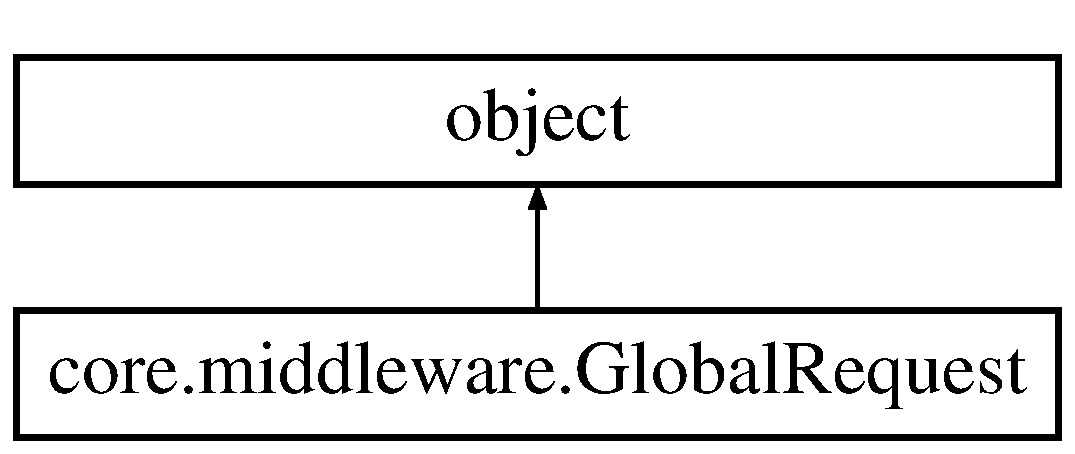
\includegraphics[height=2.000000cm]{classcore_1_1middleware_1_1GlobalRequest}
\end{center}
\end{figure}
\subsection*{Public Member Functions}
\begin{DoxyCompactItemize}
\item 
def \hyperlink{classcore_1_1middleware_1_1GlobalRequest_a16dcd9fd5dc1fb106d99cc4882808975}{process\-\_\-request}
\item 
def \hyperlink{classcore_1_1middleware_1_1GlobalRequest_a38cbb5a1292527739123289504048485}{process\-\_\-response}
\end{DoxyCompactItemize}
\subsection*{Static Public Member Functions}
\begin{DoxyCompactItemize}
\item 
def \hyperlink{classcore_1_1middleware_1_1GlobalRequest_a9e7b4d4549a961a8914f617cc9987778}{get\-\_\-request}
\end{DoxyCompactItemize}


\subsection{Detailed Description}
Thread-\/safe middleware that makes the current request object available globally. 

\href{http://djangosnippets.org/snippets/2853/}{\tt http\-://djangosnippets.\-org/snippets/2853/} 

\subsection{Member Function Documentation}
\hypertarget{classcore_1_1middleware_1_1GlobalRequest_a9e7b4d4549a961a8914f617cc9987778}{\index{core\-::middleware\-::\-Global\-Request@{core\-::middleware\-::\-Global\-Request}!get\-\_\-request@{get\-\_\-request}}
\index{get\-\_\-request@{get\-\_\-request}!core::middleware::GlobalRequest@{core\-::middleware\-::\-Global\-Request}}
\subsubsection[{get\-\_\-request}]{\setlength{\rightskip}{0pt plus 5cm}def core.\-middleware.\-Global\-Request.\-get\-\_\-request (
\begin{DoxyParamCaption}
{}
\end{DoxyParamCaption}
)\hspace{0.3cm}{\ttfamily [static]}}}\label{classcore_1_1middleware_1_1GlobalRequest_a9e7b4d4549a961a8914f617cc9987778}
\hypertarget{classcore_1_1middleware_1_1GlobalRequest_a16dcd9fd5dc1fb106d99cc4882808975}{\index{core\-::middleware\-::\-Global\-Request@{core\-::middleware\-::\-Global\-Request}!process\-\_\-request@{process\-\_\-request}}
\index{process\-\_\-request@{process\-\_\-request}!core::middleware::GlobalRequest@{core\-::middleware\-::\-Global\-Request}}
\subsubsection[{process\-\_\-request}]{\setlength{\rightskip}{0pt plus 5cm}def core.\-middleware.\-Global\-Request.\-process\-\_\-request (
\begin{DoxyParamCaption}
\item[{}]{self, }
\item[{}]{request}
\end{DoxyParamCaption}
)}}\label{classcore_1_1middleware_1_1GlobalRequest_a16dcd9fd5dc1fb106d99cc4882808975}
\hypertarget{classcore_1_1middleware_1_1GlobalRequest_a38cbb5a1292527739123289504048485}{\index{core\-::middleware\-::\-Global\-Request@{core\-::middleware\-::\-Global\-Request}!process\-\_\-response@{process\-\_\-response}}
\index{process\-\_\-response@{process\-\_\-response}!core::middleware::GlobalRequest@{core\-::middleware\-::\-Global\-Request}}
\subsubsection[{process\-\_\-response}]{\setlength{\rightskip}{0pt plus 5cm}def core.\-middleware.\-Global\-Request.\-process\-\_\-response (
\begin{DoxyParamCaption}
\item[{}]{self, }
\item[{}]{request, }
\item[{}]{response}
\end{DoxyParamCaption}
)}}\label{classcore_1_1middleware_1_1GlobalRequest_a38cbb5a1292527739123289504048485}


The documentation for this class was generated from the following file\-:\begin{DoxyCompactItemize}
\item 
/wepo/core/middleware/\hyperlink{core_2middleware_2____init_____8py}{\-\_\-\-\_\-init\-\_\-\-\_\-.\-py}\end{DoxyCompactItemize}

\hypertarget{classcore_1_1models_1_1Group}{\section{core.\-models.\-Group Class Reference}
\label{classcore_1_1models_1_1Group}\index{core.\-models.\-Group@{core.\-models.\-Group}}
}


Groups.  


Inheritance diagram for core.\-models.\-Group\-:\begin{figure}[H]
\begin{center}
\leavevmode
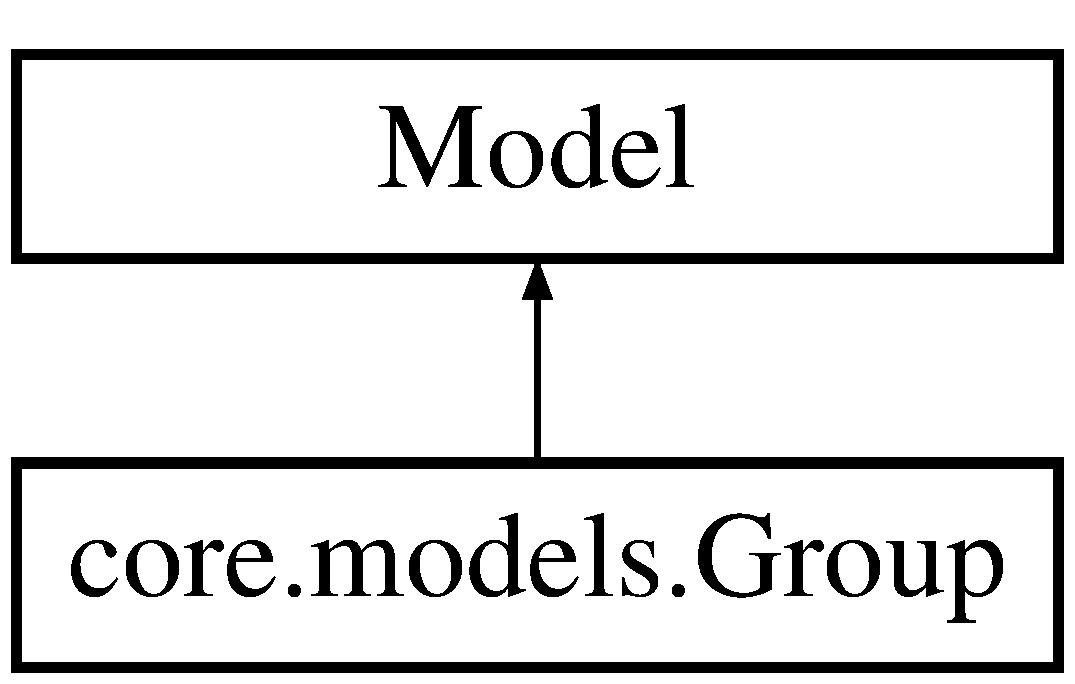
\includegraphics[height=2.000000cm]{classcore_1_1models_1_1Group}
\end{center}
\end{figure}
\subsection*{Classes}
\begin{DoxyCompactItemize}
\item 
class \hyperlink{classcore_1_1models_1_1Group_1_1Meta}{Meta}
\end{DoxyCompactItemize}
\subsection*{Public Member Functions}
\begin{DoxyCompactItemize}
\item 
def \hyperlink{classcore_1_1models_1_1Group_a8764b5ef1972100111dd0d33c95f417a}{\-\_\-\-\_\-unicode\-\_\-\-\_\-}
\item 
def \hyperlink{classcore_1_1models_1_1Group_ab867392abab3272052c7bce26c5fbea4}{save}
\begin{DoxyCompactList}\small\item\em Custom save method. \end{DoxyCompactList}\item 
def \hyperlink{classcore_1_1models_1_1Group_a0ff6af440da1ef342556e893de28537b}{get\-\_\-seo}
\begin{DoxyCompactList}\small\item\em Get seo link. \end{DoxyCompactList}\end{DoxyCompactItemize}
\subsection*{Public Attributes}
\begin{DoxyCompactItemize}
\item 
\hyperlink{classcore_1_1models_1_1Group_a0e455bf93e8ef057105e84940632e65e}{key\-\_\-name}
\end{DoxyCompactItemize}
\subsection*{Static Public Attributes}
\begin{DoxyCompactItemize}
\item 
tuple \hyperlink{classcore_1_1models_1_1Group_a4cdd32a2664af27834735b341b78422a}{name} = dmodels.\-Char\-Field(max\-\_\-length=64)
\begin{DoxyCompactList}\small\item\em Name of the group. \end{DoxyCompactList}\item 
tuple \hyperlink{classcore_1_1models_1_1Group_a0e455bf93e8ef057105e84940632e65e}{key\-\_\-name} = dmodels.\-Char\-Field(max\-\_\-length=64, db\-\_\-index=True)
\begin{DoxyCompactList}\small\item\em Unique identifier of the group. \end{DoxyCompactList}\item 
tuple \hyperlink{classcore_1_1models_1_1Group_af6dd4a8383b686c8eb65fdb5310983a6}{permissions} = \hyperlink{classcore_1_1fields_1_1JsonField}{Json\-Field}(null=True, blank=True)
\begin{DoxyCompactList}\small\item\em List of permissions in group. \end{DoxyCompactList}\end{DoxyCompactItemize}


\subsection{Detailed Description}
Groups. 

To group specified permissions. 

\subsection{Member Function Documentation}
\hypertarget{classcore_1_1models_1_1Group_a8764b5ef1972100111dd0d33c95f417a}{\index{core\-::models\-::\-Group@{core\-::models\-::\-Group}!\-\_\-\-\_\-unicode\-\_\-\-\_\-@{\-\_\-\-\_\-unicode\-\_\-\-\_\-}}
\index{\-\_\-\-\_\-unicode\-\_\-\-\_\-@{\-\_\-\-\_\-unicode\-\_\-\-\_\-}!core::models::Group@{core\-::models\-::\-Group}}
\subsubsection[{\-\_\-\-\_\-unicode\-\_\-\-\_\-}]{\setlength{\rightskip}{0pt plus 5cm}def core.\-models.\-Group.\-\_\-\-\_\-unicode\-\_\-\-\_\- (
\begin{DoxyParamCaption}
\item[{}]{self}
\end{DoxyParamCaption}
)}}\label{classcore_1_1models_1_1Group_a8764b5ef1972100111dd0d33c95f417a}
\hypertarget{classcore_1_1models_1_1Group_a0ff6af440da1ef342556e893de28537b}{\index{core\-::models\-::\-Group@{core\-::models\-::\-Group}!get\-\_\-seo@{get\-\_\-seo}}
\index{get\-\_\-seo@{get\-\_\-seo}!core::models::Group@{core\-::models\-::\-Group}}
\subsubsection[{get\-\_\-seo}]{\setlength{\rightskip}{0pt plus 5cm}def core.\-models.\-Group.\-get\-\_\-seo (
\begin{DoxyParamCaption}
\item[{}]{self}
\end{DoxyParamCaption}
)}}\label{classcore_1_1models_1_1Group_a0ff6af440da1ef342556e893de28537b}


Get seo link. 

\hypertarget{classcore_1_1models_1_1Group_ab867392abab3272052c7bce26c5fbea4}{\index{core\-::models\-::\-Group@{core\-::models\-::\-Group}!save@{save}}
\index{save@{save}!core::models::Group@{core\-::models\-::\-Group}}
\subsubsection[{save}]{\setlength{\rightskip}{0pt plus 5cm}def core.\-models.\-Group.\-save (
\begin{DoxyParamCaption}
\item[{}]{self, }
\item[{}]{force\-\_\-insert = {\ttfamily False}, }
\item[{}]{force\-\_\-update = {\ttfamily False}, }
\item[{}]{using = {\ttfamily None}, }
\item[{}]{update\-\_\-fields = {\ttfamily None}}
\end{DoxyParamCaption}
)}}\label{classcore_1_1models_1_1Group_ab867392abab3272052c7bce26c5fbea4}


Custom save method. 



\subsection{Member Data Documentation}
\hypertarget{classcore_1_1models_1_1Group_a0e455bf93e8ef057105e84940632e65e}{\index{core\-::models\-::\-Group@{core\-::models\-::\-Group}!key\-\_\-name@{key\-\_\-name}}
\index{key\-\_\-name@{key\-\_\-name}!core::models::Group@{core\-::models\-::\-Group}}
\subsubsection[{key\-\_\-name}]{\setlength{\rightskip}{0pt plus 5cm}core.\-models.\-Group.\-key\-\_\-name = dmodels.\-Char\-Field(max\-\_\-length=64, db\-\_\-index=True)\hspace{0.3cm}{\ttfamily [static]}}}\label{classcore_1_1models_1_1Group_a0e455bf93e8ef057105e84940632e65e}


Unique identifier of the group. 

\hypertarget{classcore_1_1models_1_1Group_a0e455bf93e8ef057105e84940632e65e}{\index{core\-::models\-::\-Group@{core\-::models\-::\-Group}!key\-\_\-name@{key\-\_\-name}}
\index{key\-\_\-name@{key\-\_\-name}!core::models::Group@{core\-::models\-::\-Group}}
\subsubsection[{key\-\_\-name}]{\setlength{\rightskip}{0pt plus 5cm}core.\-models.\-Group.\-key\-\_\-name}}\label{classcore_1_1models_1_1Group_a0e455bf93e8ef057105e84940632e65e}
\hypertarget{classcore_1_1models_1_1Group_a4cdd32a2664af27834735b341b78422a}{\index{core\-::models\-::\-Group@{core\-::models\-::\-Group}!name@{name}}
\index{name@{name}!core::models::Group@{core\-::models\-::\-Group}}
\subsubsection[{name}]{\setlength{\rightskip}{0pt plus 5cm}core.\-models.\-Group.\-name = dmodels.\-Char\-Field(max\-\_\-length=64)\hspace{0.3cm}{\ttfamily [static]}}}\label{classcore_1_1models_1_1Group_a4cdd32a2664af27834735b341b78422a}


Name of the group. 

\hypertarget{classcore_1_1models_1_1Group_af6dd4a8383b686c8eb65fdb5310983a6}{\index{core\-::models\-::\-Group@{core\-::models\-::\-Group}!permissions@{permissions}}
\index{permissions@{permissions}!core::models::Group@{core\-::models\-::\-Group}}
\subsubsection[{permissions}]{\setlength{\rightskip}{0pt plus 5cm}core.\-models.\-Group.\-permissions = {\bf Json\-Field}(null=True, blank=True)\hspace{0.3cm}{\ttfamily [static]}}}\label{classcore_1_1models_1_1Group_af6dd4a8383b686c8eb65fdb5310983a6}


List of permissions in group. 



The documentation for this class was generated from the following file\-:\begin{DoxyCompactItemize}
\item 
/wepo/core/\hyperlink{models_8py}{models.\-py}\end{DoxyCompactItemize}

\hypertarget{classcore_1_1helper_1_1response__help_1_1HttpRedirect}{\section{core.\-helper.\-response\-\_\-help.\-Http\-Redirect Class Reference}
\label{classcore_1_1helper_1_1response__help_1_1HttpRedirect}\index{core.\-helper.\-response\-\_\-help.\-Http\-Redirect@{core.\-helper.\-response\-\_\-help.\-Http\-Redirect}}
}


Redirect -\/ basic redirect helper.  


\subsection*{Public Member Functions}
\begin{DoxyCompactItemize}
\item 
def \hyperlink{classcore_1_1helper_1_1response__help_1_1HttpRedirect_a506632087d9afabe2fbdcbe0dd135398}{\-\_\-\-\_\-init\-\_\-\-\_\-}
\end{DoxyCompactItemize}
\subsection*{Public Attributes}
\begin{DoxyCompactItemize}
\item 
\hyperlink{classcore_1_1helper_1_1response__help_1_1HttpRedirect_a5f476d0180feb4e05d1b20a29a24d3cf}{url}
\end{DoxyCompactItemize}


\subsection{Detailed Description}
Redirect -\/ basic redirect helper. 

\subsection{Constructor \& Destructor Documentation}
\hypertarget{classcore_1_1helper_1_1response__help_1_1HttpRedirect_a506632087d9afabe2fbdcbe0dd135398}{\index{core\-::helper\-::response\-\_\-help\-::\-Http\-Redirect@{core\-::helper\-::response\-\_\-help\-::\-Http\-Redirect}!\-\_\-\-\_\-init\-\_\-\-\_\-@{\-\_\-\-\_\-init\-\_\-\-\_\-}}
\index{\-\_\-\-\_\-init\-\_\-\-\_\-@{\-\_\-\-\_\-init\-\_\-\-\_\-}!core::helper::response_help::HttpRedirect@{core\-::helper\-::response\-\_\-help\-::\-Http\-Redirect}}
\subsubsection[{\-\_\-\-\_\-init\-\_\-\-\_\-}]{\setlength{\rightskip}{0pt plus 5cm}def core.\-helper.\-response\-\_\-help.\-Http\-Redirect.\-\_\-\-\_\-init\-\_\-\-\_\- (
\begin{DoxyParamCaption}
\item[{}]{self, }
\item[{}]{url}
\end{DoxyParamCaption}
)}}\label{classcore_1_1helper_1_1response__help_1_1HttpRedirect_a506632087d9afabe2fbdcbe0dd135398}


\subsection{Member Data Documentation}
\hypertarget{classcore_1_1helper_1_1response__help_1_1HttpRedirect_a5f476d0180feb4e05d1b20a29a24d3cf}{\index{core\-::helper\-::response\-\_\-help\-::\-Http\-Redirect@{core\-::helper\-::response\-\_\-help\-::\-Http\-Redirect}!url@{url}}
\index{url@{url}!core::helper::response_help::HttpRedirect@{core\-::helper\-::response\-\_\-help\-::\-Http\-Redirect}}
\subsubsection[{url}]{\setlength{\rightskip}{0pt plus 5cm}core.\-helper.\-response\-\_\-help.\-Http\-Redirect.\-url}}\label{classcore_1_1helper_1_1response__help_1_1HttpRedirect_a5f476d0180feb4e05d1b20a29a24d3cf}


The documentation for this class was generated from the following file\-:\begin{DoxyCompactItemize}
\item 
/wepo/core/helper/\hyperlink{response__help_8py}{response\-\_\-help.\-py}\end{DoxyCompactItemize}

\hypertarget{classcore_1_1install_1_1Install}{\section{core.\-install.\-Install Class Reference}
\label{classcore_1_1install_1_1Install}\index{core.\-install.\-Install@{core.\-install.\-Install}}
}


\hyperlink{classcore_1_1install_1_1Install}{Install} objects.  


\subsection*{Public Member Functions}
\begin{DoxyCompactItemize}
\item 
def \hyperlink{classcore_1_1install_1_1Install_a26278942ad9db88286180b1bee3e3042}{install}
\begin{DoxyCompactList}\small\item\em install data \end{DoxyCompactList}\item 
def \hyperlink{classcore_1_1install_1_1Install_a42a57a74329d83206317ea24a55d0f8f}{load\-\_\-csv}
\begin{DoxyCompactList}\small\item\em Import data from. \end{DoxyCompactList}\end{DoxyCompactItemize}


\subsection{Detailed Description}
\hyperlink{classcore_1_1install_1_1Install}{Install} objects. 

\subsection{Member Function Documentation}
\hypertarget{classcore_1_1install_1_1Install_a26278942ad9db88286180b1bee3e3042}{\index{core\-::install\-::\-Install@{core\-::install\-::\-Install}!install@{install}}
\index{install@{install}!core::install::Install@{core\-::install\-::\-Install}}
\subsubsection[{install}]{\setlength{\rightskip}{0pt plus 5cm}def core.\-install.\-Install.\-install (
\begin{DoxyParamCaption}
\item[{}]{self, }
\item[{}]{allowed = {\ttfamily \mbox{[}\mbox{]}}}
\end{DoxyParamCaption}
)}}\label{classcore_1_1install_1_1Install_a26278942ad9db88286180b1bee3e3042}


install data 

\hypertarget{classcore_1_1install_1_1Install_a42a57a74329d83206317ea24a55d0f8f}{\index{core\-::install\-::\-Install@{core\-::install\-::\-Install}!load\-\_\-csv@{load\-\_\-csv}}
\index{load\-\_\-csv@{load\-\_\-csv}!core::install::Install@{core\-::install\-::\-Install}}
\subsubsection[{load\-\_\-csv}]{\setlength{\rightskip}{0pt plus 5cm}def core.\-install.\-Install.\-load\-\_\-csv (
\begin{DoxyParamCaption}
\item[{}]{self}
\end{DoxyParamCaption}
)}}\label{classcore_1_1install_1_1Install_a42a57a74329d83206317ea24a55d0f8f}


Import data from. 



The documentation for this class was generated from the following file\-:\begin{DoxyCompactItemize}
\item 
/wepo/core/install/\hyperlink{core_2install_2____init_____8py}{\-\_\-\-\_\-init\-\_\-\-\_\-.\-py}\end{DoxyCompactItemize}

\hypertarget{classcore_1_1fields_1_1JsonField}{\section{core.\-fields.\-Json\-Field Class Reference}
\label{classcore_1_1fields_1_1JsonField}\index{core.\-fields.\-Json\-Field@{core.\-fields.\-Json\-Field}}
}


J\-S\-O\-N\-Field is a generic textfield that neatly serializes/unserializes J\-S\-O\-N objects seamlessly.  


Inheritance diagram for core.\-fields.\-Json\-Field\-:\begin{figure}[H]
\begin{center}
\leavevmode
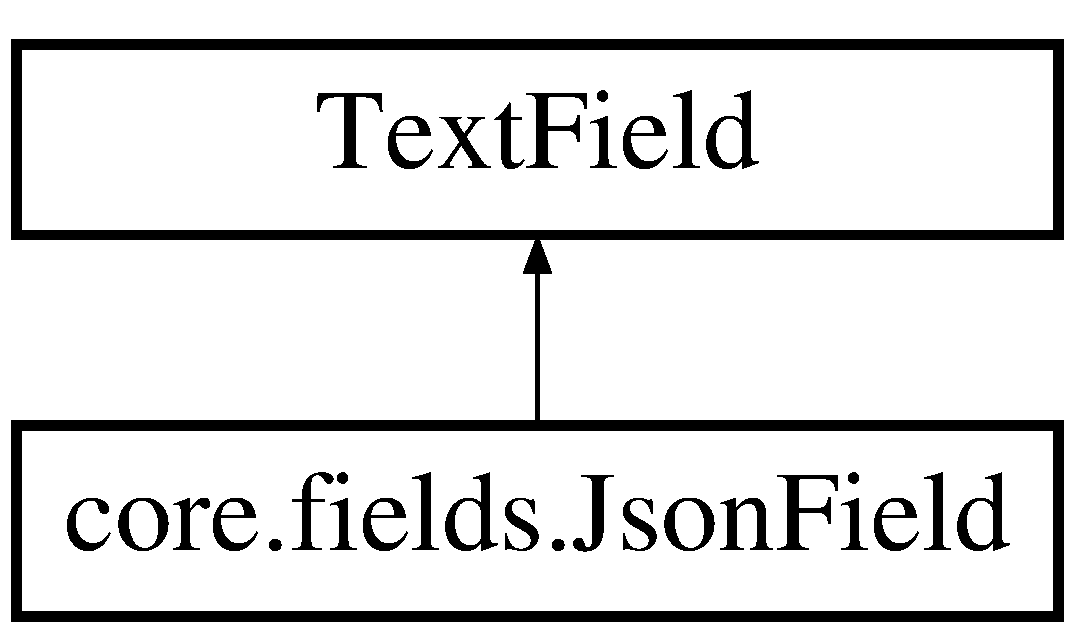
\includegraphics[height=2.000000cm]{classcore_1_1fields_1_1JsonField}
\end{center}
\end{figure}
\subsection*{Public Member Functions}
\begin{DoxyCompactItemize}
\item 
def \hyperlink{classcore_1_1fields_1_1JsonField_abac7ef742861c6a1bb4d7b738617a239}{get\-\_\-custom\-\_\-internal\-\_\-type}
\item 
def \hyperlink{classcore_1_1fields_1_1JsonField_a7b9074a7adf9567b61f27c498f6252e3}{to\-\_\-python}
\item 
def \hyperlink{classcore_1_1fields_1_1JsonField_a67375a04019233035864ce6935498d0b}{get\-\_\-db\-\_\-prep\-\_\-save}
\end{DoxyCompactItemize}


\subsection{Detailed Description}
J\-S\-O\-N\-Field is a generic textfield that neatly serializes/unserializes J\-S\-O\-N objects seamlessly. 

\subsection{Member Function Documentation}
\hypertarget{classcore_1_1fields_1_1JsonField_abac7ef742861c6a1bb4d7b738617a239}{\index{core\-::fields\-::\-Json\-Field@{core\-::fields\-::\-Json\-Field}!get\-\_\-custom\-\_\-internal\-\_\-type@{get\-\_\-custom\-\_\-internal\-\_\-type}}
\index{get\-\_\-custom\-\_\-internal\-\_\-type@{get\-\_\-custom\-\_\-internal\-\_\-type}!core::fields::JsonField@{core\-::fields\-::\-Json\-Field}}
\subsubsection[{get\-\_\-custom\-\_\-internal\-\_\-type}]{\setlength{\rightskip}{0pt plus 5cm}def core.\-fields.\-Json\-Field.\-get\-\_\-custom\-\_\-internal\-\_\-type (
\begin{DoxyParamCaption}
\item[{}]{self}
\end{DoxyParamCaption}
)}}\label{classcore_1_1fields_1_1JsonField_abac7ef742861c6a1bb4d7b738617a239}
\hypertarget{classcore_1_1fields_1_1JsonField_a67375a04019233035864ce6935498d0b}{\index{core\-::fields\-::\-Json\-Field@{core\-::fields\-::\-Json\-Field}!get\-\_\-db\-\_\-prep\-\_\-save@{get\-\_\-db\-\_\-prep\-\_\-save}}
\index{get\-\_\-db\-\_\-prep\-\_\-save@{get\-\_\-db\-\_\-prep\-\_\-save}!core::fields::JsonField@{core\-::fields\-::\-Json\-Field}}
\subsubsection[{get\-\_\-db\-\_\-prep\-\_\-save}]{\setlength{\rightskip}{0pt plus 5cm}def core.\-fields.\-Json\-Field.\-get\-\_\-db\-\_\-prep\-\_\-save (
\begin{DoxyParamCaption}
\item[{}]{self, }
\item[{}]{value, }
\item[{}]{connection}
\end{DoxyParamCaption}
)}}\label{classcore_1_1fields_1_1JsonField_a67375a04019233035864ce6935498d0b}
\hypertarget{classcore_1_1fields_1_1JsonField_a7b9074a7adf9567b61f27c498f6252e3}{\index{core\-::fields\-::\-Json\-Field@{core\-::fields\-::\-Json\-Field}!to\-\_\-python@{to\-\_\-python}}
\index{to\-\_\-python@{to\-\_\-python}!core::fields::JsonField@{core\-::fields\-::\-Json\-Field}}
\subsubsection[{to\-\_\-python}]{\setlength{\rightskip}{0pt plus 5cm}def core.\-fields.\-Json\-Field.\-to\-\_\-python (
\begin{DoxyParamCaption}
\item[{}]{self, }
\item[{}]{value}
\end{DoxyParamCaption}
)}}\label{classcore_1_1fields_1_1JsonField_a7b9074a7adf9567b61f27c498f6252e3}


The documentation for this class was generated from the following file\-:\begin{DoxyCompactItemize}
\item 
/wepo/core/\hyperlink{fields_8py}{fields.\-py}\end{DoxyCompactItemize}

\hypertarget{classcore_1_1json__cache_1_1MemcachedCacheJSON}{\section{core.\-json\-\_\-cache.\-Memcached\-Cache\-J\-S\-O\-N Class Reference}
\label{classcore_1_1json__cache_1_1MemcachedCacheJSON}\index{core.\-json\-\_\-cache.\-Memcached\-Cache\-J\-S\-O\-N@{core.\-json\-\_\-cache.\-Memcached\-Cache\-J\-S\-O\-N}}
}


Memcache store with J\-S\-O\-N serialization.  


Inheritance diagram for core.\-json\-\_\-cache.\-Memcached\-Cache\-J\-S\-O\-N\-:\begin{figure}[H]
\begin{center}
\leavevmode
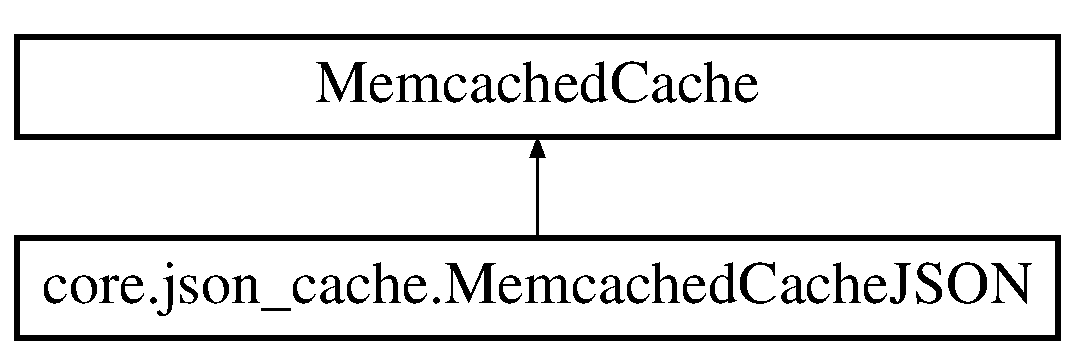
\includegraphics[height=2.000000cm]{classcore_1_1json__cache_1_1MemcachedCacheJSON}
\end{center}
\end{figure}


\subsection{Detailed Description}
Memcache store with J\-S\-O\-N serialization. 

We want node.\-js applications to be able to read the stuff Django stores to memcached so instead of pickling the data we'll serialize it to json. This is kind of a hack because looking at python-\/memcached's source it seems {\itshape really} intent on using pickle. 

The documentation for this class was generated from the following file\-:\begin{DoxyCompactItemize}
\item 
/wepo/core/\hyperlink{json__cache_8py}{json\-\_\-cache.\-py}\end{DoxyCompactItemize}

\hypertarget{classcore_1_1models_1_1Menu}{\section{core.\-models.\-Menu Class Reference}
\label{classcore_1_1models_1_1Menu}\index{core.\-models.\-Menu@{core.\-models.\-Menu}}
}


\hyperlink{classcore_1_1models_1_1Menu}{Menu}.  


Inheritance diagram for core.\-models.\-Menu\-:\begin{figure}[H]
\begin{center}
\leavevmode
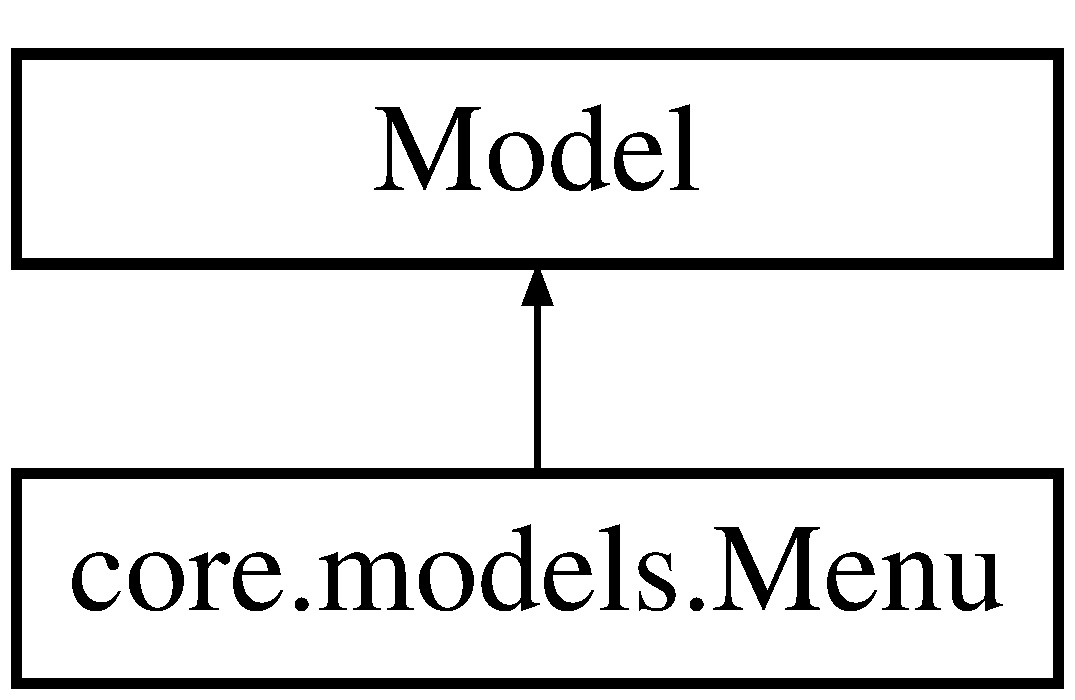
\includegraphics[height=2.000000cm]{classcore_1_1models_1_1Menu}
\end{center}
\end{figure}
\subsection*{Classes}
\begin{DoxyCompactItemize}
\item 
class \hyperlink{classcore_1_1models_1_1Menu_1_1Meta}{Meta}
\end{DoxyCompactItemize}
\subsection*{Public Member Functions}
\begin{DoxyCompactItemize}
\item 
def \hyperlink{classcore_1_1models_1_1Menu_a2d312c756cc18acc82c71d7ca7e3a2c7}{\-\_\-\-\_\-unicode\-\_\-\-\_\-}
\item 
def \hyperlink{classcore_1_1models_1_1Menu_ad0df5ff467b92ce10a1fa4b1ed2a7095}{save}
\begin{DoxyCompactList}\small\item\em Custom save method. \end{DoxyCompactList}\item 
def \hyperlink{classcore_1_1models_1_1Menu_ad6879fe999e825fca1132410a54ecb76}{get\-\_\-seo}
\begin{DoxyCompactList}\small\item\em Get seo link. \end{DoxyCompactList}\end{DoxyCompactItemize}
\subsection*{Public Attributes}
\begin{DoxyCompactItemize}
\item 
\hyperlink{classcore_1_1models_1_1Menu_a68d1ce76cccad9def97d24afe21ad728}{key\-\_\-name}
\end{DoxyCompactItemize}
\subsection*{Static Public Attributes}
\begin{DoxyCompactItemize}
\item 
tuple \hyperlink{classcore_1_1models_1_1Menu_a6782a44a3141438c0eca3fd2bcff4e9c}{name} = dmodels.\-Char\-Field(max\-\_\-length=64)
\begin{DoxyCompactList}\small\item\em Name of the menu. \end{DoxyCompactList}\item 
tuple \hyperlink{classcore_1_1models_1_1Menu_a68d1ce76cccad9def97d24afe21ad728}{key\-\_\-name} = dmodels.\-Char\-Field(max\-\_\-length=64, db\-\_\-index=True)
\begin{DoxyCompactList}\small\item\em Unique identifier of the menu. \end{DoxyCompactList}\end{DoxyCompactItemize}


\subsection{Detailed Description}
\hyperlink{classcore_1_1models_1_1Menu}{Menu}. 

(Main menu, Admin side menu, Admin top menu, ...) 

\subsection{Member Function Documentation}
\hypertarget{classcore_1_1models_1_1Menu_a2d312c756cc18acc82c71d7ca7e3a2c7}{\index{core\-::models\-::\-Menu@{core\-::models\-::\-Menu}!\-\_\-\-\_\-unicode\-\_\-\-\_\-@{\-\_\-\-\_\-unicode\-\_\-\-\_\-}}
\index{\-\_\-\-\_\-unicode\-\_\-\-\_\-@{\-\_\-\-\_\-unicode\-\_\-\-\_\-}!core::models::Menu@{core\-::models\-::\-Menu}}
\subsubsection[{\-\_\-\-\_\-unicode\-\_\-\-\_\-}]{\setlength{\rightskip}{0pt plus 5cm}def core.\-models.\-Menu.\-\_\-\-\_\-unicode\-\_\-\-\_\- (
\begin{DoxyParamCaption}
\item[{}]{self}
\end{DoxyParamCaption}
)}}\label{classcore_1_1models_1_1Menu_a2d312c756cc18acc82c71d7ca7e3a2c7}
\hypertarget{classcore_1_1models_1_1Menu_ad6879fe999e825fca1132410a54ecb76}{\index{core\-::models\-::\-Menu@{core\-::models\-::\-Menu}!get\-\_\-seo@{get\-\_\-seo}}
\index{get\-\_\-seo@{get\-\_\-seo}!core::models::Menu@{core\-::models\-::\-Menu}}
\subsubsection[{get\-\_\-seo}]{\setlength{\rightskip}{0pt plus 5cm}def core.\-models.\-Menu.\-get\-\_\-seo (
\begin{DoxyParamCaption}
\item[{}]{self}
\end{DoxyParamCaption}
)}}\label{classcore_1_1models_1_1Menu_ad6879fe999e825fca1132410a54ecb76}


Get seo link. 

\hypertarget{classcore_1_1models_1_1Menu_ad0df5ff467b92ce10a1fa4b1ed2a7095}{\index{core\-::models\-::\-Menu@{core\-::models\-::\-Menu}!save@{save}}
\index{save@{save}!core::models::Menu@{core\-::models\-::\-Menu}}
\subsubsection[{save}]{\setlength{\rightskip}{0pt plus 5cm}def core.\-models.\-Menu.\-save (
\begin{DoxyParamCaption}
\item[{}]{self, }
\item[{}]{force\-\_\-insert = {\ttfamily False}, }
\item[{}]{force\-\_\-update = {\ttfamily False}, }
\item[{}]{using = {\ttfamily None}, }
\item[{}]{update\-\_\-fields = {\ttfamily None}}
\end{DoxyParamCaption}
)}}\label{classcore_1_1models_1_1Menu_ad0df5ff467b92ce10a1fa4b1ed2a7095}


Custom save method. 



\subsection{Member Data Documentation}
\hypertarget{classcore_1_1models_1_1Menu_a68d1ce76cccad9def97d24afe21ad728}{\index{core\-::models\-::\-Menu@{core\-::models\-::\-Menu}!key\-\_\-name@{key\-\_\-name}}
\index{key\-\_\-name@{key\-\_\-name}!core::models::Menu@{core\-::models\-::\-Menu}}
\subsubsection[{key\-\_\-name}]{\setlength{\rightskip}{0pt plus 5cm}core.\-models.\-Menu.\-key\-\_\-name = dmodels.\-Char\-Field(max\-\_\-length=64, db\-\_\-index=True)\hspace{0.3cm}{\ttfamily [static]}}}\label{classcore_1_1models_1_1Menu_a68d1ce76cccad9def97d24afe21ad728}


Unique identifier of the menu. 

\hypertarget{classcore_1_1models_1_1Menu_a68d1ce76cccad9def97d24afe21ad728}{\index{core\-::models\-::\-Menu@{core\-::models\-::\-Menu}!key\-\_\-name@{key\-\_\-name}}
\index{key\-\_\-name@{key\-\_\-name}!core::models::Menu@{core\-::models\-::\-Menu}}
\subsubsection[{key\-\_\-name}]{\setlength{\rightskip}{0pt plus 5cm}core.\-models.\-Menu.\-key\-\_\-name}}\label{classcore_1_1models_1_1Menu_a68d1ce76cccad9def97d24afe21ad728}
\hypertarget{classcore_1_1models_1_1Menu_a6782a44a3141438c0eca3fd2bcff4e9c}{\index{core\-::models\-::\-Menu@{core\-::models\-::\-Menu}!name@{name}}
\index{name@{name}!core::models::Menu@{core\-::models\-::\-Menu}}
\subsubsection[{name}]{\setlength{\rightskip}{0pt plus 5cm}core.\-models.\-Menu.\-name = dmodels.\-Char\-Field(max\-\_\-length=64)\hspace{0.3cm}{\ttfamily [static]}}}\label{classcore_1_1models_1_1Menu_a6782a44a3141438c0eca3fd2bcff4e9c}


Name of the menu. 



The documentation for this class was generated from the following file\-:\begin{DoxyCompactItemize}
\item 
/wepo/core/\hyperlink{models_8py}{models.\-py}\end{DoxyCompactItemize}

\hypertarget{classcore_1_1models_1_1MenuItem}{\section{core.\-models.\-Menu\-Item Class Reference}
\label{classcore_1_1models_1_1MenuItem}\index{core.\-models.\-Menu\-Item@{core.\-models.\-Menu\-Item}}
}


\hyperlink{classcore_1_1models_1_1Menu}{Menu} item.  


Inheritance diagram for core.\-models.\-Menu\-Item\-:\begin{figure}[H]
\begin{center}
\leavevmode
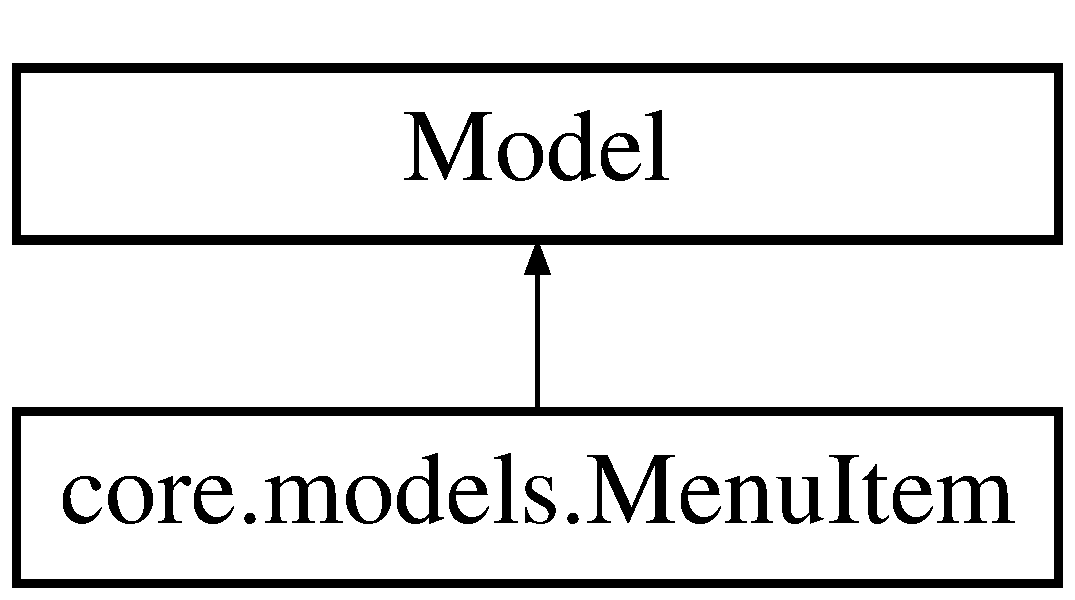
\includegraphics[height=2.000000cm]{classcore_1_1models_1_1MenuItem}
\end{center}
\end{figure}
\subsection*{Classes}
\begin{DoxyCompactItemize}
\item 
class \hyperlink{classcore_1_1models_1_1MenuItem_1_1Meta}{Meta}
\end{DoxyCompactItemize}
\subsection*{Public Member Functions}
\begin{DoxyCompactItemize}
\item 
def \hyperlink{classcore_1_1models_1_1MenuItem_a7ca6064d82c1e02ddf732fccb5d1430b}{\-\_\-\-\_\-unicode\-\_\-\-\_\-}
\item 
def \hyperlink{classcore_1_1models_1_1MenuItem_ab51a5ab563ed2c10ab0a74342a1b4197}{save}
\begin{DoxyCompactList}\small\item\em Custom save method. \end{DoxyCompactList}\item 
def \hyperlink{classcore_1_1models_1_1MenuItem_a85b4e94e816f9575ad9a950c7e01d9cc}{get\-\_\-seo}
\begin{DoxyCompactList}\small\item\em Get seo link. \end{DoxyCompactList}\end{DoxyCompactItemize}
\subsection*{Public Attributes}
\begin{DoxyCompactItemize}
\item 
\hyperlink{classcore_1_1models_1_1MenuItem_a6eccff1165c95be4b9c0efee213e3878}{key\-\_\-name}
\end{DoxyCompactItemize}
\subsection*{Static Public Attributes}
\begin{DoxyCompactItemize}
\item 
tuple \hyperlink{classcore_1_1models_1_1MenuItem_ab3946f967b3a1fce02d39c5ecb2185f5}{name} = dmodels.\-Char\-Field(max\-\_\-length=255)
\begin{DoxyCompactList}\small\item\em Name of the menu item. \end{DoxyCompactList}\item 
tuple \hyperlink{classcore_1_1models_1_1MenuItem_a6eccff1165c95be4b9c0efee213e3878}{key\-\_\-name} = dmodels.\-Char\-Field(max\-\_\-length=255, db\-\_\-index=True)
\begin{DoxyCompactList}\small\item\em Unique identifier of the menu item. \end{DoxyCompactList}\item 
tuple \hyperlink{classcore_1_1models_1_1MenuItem_a0ed621cf4f336eee94ee6af73f138add}{seo} = dmodels.\-Foreign\-Key(\hyperlink{classcore_1_1models_1_1Seo}{Seo}, null=True, blank=True)
\begin{DoxyCompactList}\small\item\em \hyperlink{classcore_1_1models_1_1Seo}{Seo} link, linked to the menu item. \end{DoxyCompactList}\item 
tuple \hyperlink{classcore_1_1models_1_1MenuItem_a05a0b2b1302e5a8e224ae29a4edbe93b}{url} = dmodels.\-U\-R\-L\-Field()
\begin{DoxyCompactList}\small\item\em Extra menu item url. \end{DoxyCompactList}\item 
tuple \hyperlink{classcore_1_1models_1_1MenuItem_ac284a37490aad36640bd848f29466232}{parent} = dmodels.\-Foreign\-Key('self', null=True, blank=True)
\begin{DoxyCompactList}\small\item\em Parent menu item. \end{DoxyCompactList}\item 
tuple \hyperlink{classcore_1_1models_1_1MenuItem_afebbc45130eae0cea9c5095ef6cd98b1}{menu} = dmodels.\-Foreign\-Key(\hyperlink{classcore_1_1models_1_1Menu}{Menu}, db\-\_\-index=True)
\begin{DoxyCompactList}\small\item\em \hyperlink{classcore_1_1models_1_1Menu}{Menu} of the relation. \end{DoxyCompactList}\item 
tuple \hyperlink{classcore_1_1models_1_1MenuItem_a82ed62dbf13487126c5bc1f458c4b67c}{sort} = dmodels.\-Positive\-Small\-Integer\-Field()
\begin{DoxyCompactList}\small\item\em Numerical position of the relation. \end{DoxyCompactList}\item 
tuple \hyperlink{classcore_1_1models_1_1MenuItem_a57fc994079c4c38d7ef278c6d364f435}{level} = dmodels.\-Positive\-Small\-Integer\-Field()
\begin{DoxyCompactList}\small\item\em Level of the relation. \end{DoxyCompactList}\item 
tuple \hyperlink{classcore_1_1models_1_1MenuItem_ad8a9b116de08fe5fb590ac565c10917a}{enabled} = dmodels.\-Boolean\-Field(default=True)
\begin{DoxyCompactList}\small\item\em Status if the relation is enabled. \end{DoxyCompactList}\end{DoxyCompactItemize}


\subsection{Detailed Description}
\hyperlink{classcore_1_1models_1_1Menu}{Menu} item. 

(Main menu, Admin side menu, Admin top menu, ...) 

\subsection{Member Function Documentation}
\hypertarget{classcore_1_1models_1_1MenuItem_a7ca6064d82c1e02ddf732fccb5d1430b}{\index{core\-::models\-::\-Menu\-Item@{core\-::models\-::\-Menu\-Item}!\-\_\-\-\_\-unicode\-\_\-\-\_\-@{\-\_\-\-\_\-unicode\-\_\-\-\_\-}}
\index{\-\_\-\-\_\-unicode\-\_\-\-\_\-@{\-\_\-\-\_\-unicode\-\_\-\-\_\-}!core::models::MenuItem@{core\-::models\-::\-Menu\-Item}}
\subsubsection[{\-\_\-\-\_\-unicode\-\_\-\-\_\-}]{\setlength{\rightskip}{0pt plus 5cm}def core.\-models.\-Menu\-Item.\-\_\-\-\_\-unicode\-\_\-\-\_\- (
\begin{DoxyParamCaption}
\item[{}]{self}
\end{DoxyParamCaption}
)}}\label{classcore_1_1models_1_1MenuItem_a7ca6064d82c1e02ddf732fccb5d1430b}
\hypertarget{classcore_1_1models_1_1MenuItem_a85b4e94e816f9575ad9a950c7e01d9cc}{\index{core\-::models\-::\-Menu\-Item@{core\-::models\-::\-Menu\-Item}!get\-\_\-seo@{get\-\_\-seo}}
\index{get\-\_\-seo@{get\-\_\-seo}!core::models::MenuItem@{core\-::models\-::\-Menu\-Item}}
\subsubsection[{get\-\_\-seo}]{\setlength{\rightskip}{0pt plus 5cm}def core.\-models.\-Menu\-Item.\-get\-\_\-seo (
\begin{DoxyParamCaption}
\item[{}]{self}
\end{DoxyParamCaption}
)}}\label{classcore_1_1models_1_1MenuItem_a85b4e94e816f9575ad9a950c7e01d9cc}


Get seo link. 

\hypertarget{classcore_1_1models_1_1MenuItem_ab51a5ab563ed2c10ab0a74342a1b4197}{\index{core\-::models\-::\-Menu\-Item@{core\-::models\-::\-Menu\-Item}!save@{save}}
\index{save@{save}!core::models::MenuItem@{core\-::models\-::\-Menu\-Item}}
\subsubsection[{save}]{\setlength{\rightskip}{0pt plus 5cm}def core.\-models.\-Menu\-Item.\-save (
\begin{DoxyParamCaption}
\item[{}]{self, }
\item[{}]{force\-\_\-insert = {\ttfamily False}, }
\item[{}]{force\-\_\-update = {\ttfamily False}, }
\item[{}]{using = {\ttfamily None}, }
\item[{}]{update\-\_\-fields = {\ttfamily None}}
\end{DoxyParamCaption}
)}}\label{classcore_1_1models_1_1MenuItem_ab51a5ab563ed2c10ab0a74342a1b4197}


Custom save method. 



\subsection{Member Data Documentation}
\hypertarget{classcore_1_1models_1_1MenuItem_ad8a9b116de08fe5fb590ac565c10917a}{\index{core\-::models\-::\-Menu\-Item@{core\-::models\-::\-Menu\-Item}!enabled@{enabled}}
\index{enabled@{enabled}!core::models::MenuItem@{core\-::models\-::\-Menu\-Item}}
\subsubsection[{enabled}]{\setlength{\rightskip}{0pt plus 5cm}core.\-models.\-Menu\-Item.\-enabled = dmodels.\-Boolean\-Field(default=True)\hspace{0.3cm}{\ttfamily [static]}}}\label{classcore_1_1models_1_1MenuItem_ad8a9b116de08fe5fb590ac565c10917a}


Status if the relation is enabled. 

\hypertarget{classcore_1_1models_1_1MenuItem_a6eccff1165c95be4b9c0efee213e3878}{\index{core\-::models\-::\-Menu\-Item@{core\-::models\-::\-Menu\-Item}!key\-\_\-name@{key\-\_\-name}}
\index{key\-\_\-name@{key\-\_\-name}!core::models::MenuItem@{core\-::models\-::\-Menu\-Item}}
\subsubsection[{key\-\_\-name}]{\setlength{\rightskip}{0pt plus 5cm}core.\-models.\-Menu\-Item.\-key\-\_\-name = dmodels.\-Char\-Field(max\-\_\-length=255, db\-\_\-index=True)\hspace{0.3cm}{\ttfamily [static]}}}\label{classcore_1_1models_1_1MenuItem_a6eccff1165c95be4b9c0efee213e3878}


Unique identifier of the menu item. 

\hypertarget{classcore_1_1models_1_1MenuItem_a6eccff1165c95be4b9c0efee213e3878}{\index{core\-::models\-::\-Menu\-Item@{core\-::models\-::\-Menu\-Item}!key\-\_\-name@{key\-\_\-name}}
\index{key\-\_\-name@{key\-\_\-name}!core::models::MenuItem@{core\-::models\-::\-Menu\-Item}}
\subsubsection[{key\-\_\-name}]{\setlength{\rightskip}{0pt plus 5cm}core.\-models.\-Menu\-Item.\-key\-\_\-name}}\label{classcore_1_1models_1_1MenuItem_a6eccff1165c95be4b9c0efee213e3878}
\hypertarget{classcore_1_1models_1_1MenuItem_a57fc994079c4c38d7ef278c6d364f435}{\index{core\-::models\-::\-Menu\-Item@{core\-::models\-::\-Menu\-Item}!level@{level}}
\index{level@{level}!core::models::MenuItem@{core\-::models\-::\-Menu\-Item}}
\subsubsection[{level}]{\setlength{\rightskip}{0pt plus 5cm}core.\-models.\-Menu\-Item.\-level = dmodels.\-Positive\-Small\-Integer\-Field()\hspace{0.3cm}{\ttfamily [static]}}}\label{classcore_1_1models_1_1MenuItem_a57fc994079c4c38d7ef278c6d364f435}


Level of the relation. 

\hypertarget{classcore_1_1models_1_1MenuItem_afebbc45130eae0cea9c5095ef6cd98b1}{\index{core\-::models\-::\-Menu\-Item@{core\-::models\-::\-Menu\-Item}!menu@{menu}}
\index{menu@{menu}!core::models::MenuItem@{core\-::models\-::\-Menu\-Item}}
\subsubsection[{menu}]{\setlength{\rightskip}{0pt plus 5cm}core.\-models.\-Menu\-Item.\-menu = dmodels.\-Foreign\-Key({\bf Menu}, db\-\_\-index=True)\hspace{0.3cm}{\ttfamily [static]}}}\label{classcore_1_1models_1_1MenuItem_afebbc45130eae0cea9c5095ef6cd98b1}


\hyperlink{classcore_1_1models_1_1Menu}{Menu} of the relation. 

\hypertarget{classcore_1_1models_1_1MenuItem_ab3946f967b3a1fce02d39c5ecb2185f5}{\index{core\-::models\-::\-Menu\-Item@{core\-::models\-::\-Menu\-Item}!name@{name}}
\index{name@{name}!core::models::MenuItem@{core\-::models\-::\-Menu\-Item}}
\subsubsection[{name}]{\setlength{\rightskip}{0pt plus 5cm}core.\-models.\-Menu\-Item.\-name = dmodels.\-Char\-Field(max\-\_\-length=255)\hspace{0.3cm}{\ttfamily [static]}}}\label{classcore_1_1models_1_1MenuItem_ab3946f967b3a1fce02d39c5ecb2185f5}


Name of the menu item. 

\hypertarget{classcore_1_1models_1_1MenuItem_ac284a37490aad36640bd848f29466232}{\index{core\-::models\-::\-Menu\-Item@{core\-::models\-::\-Menu\-Item}!parent@{parent}}
\index{parent@{parent}!core::models::MenuItem@{core\-::models\-::\-Menu\-Item}}
\subsubsection[{parent}]{\setlength{\rightskip}{0pt plus 5cm}core.\-models.\-Menu\-Item.\-parent = dmodels.\-Foreign\-Key('self', null=True, blank=True)\hspace{0.3cm}{\ttfamily [static]}}}\label{classcore_1_1models_1_1MenuItem_ac284a37490aad36640bd848f29466232}


Parent menu item. 

\hypertarget{classcore_1_1models_1_1MenuItem_a0ed621cf4f336eee94ee6af73f138add}{\index{core\-::models\-::\-Menu\-Item@{core\-::models\-::\-Menu\-Item}!seo@{seo}}
\index{seo@{seo}!core::models::MenuItem@{core\-::models\-::\-Menu\-Item}}
\subsubsection[{seo}]{\setlength{\rightskip}{0pt plus 5cm}core.\-models.\-Menu\-Item.\-seo = dmodels.\-Foreign\-Key({\bf Seo}, null=True, blank=True)\hspace{0.3cm}{\ttfamily [static]}}}\label{classcore_1_1models_1_1MenuItem_a0ed621cf4f336eee94ee6af73f138add}


\hyperlink{classcore_1_1models_1_1Seo}{Seo} link, linked to the menu item. 

\hypertarget{classcore_1_1models_1_1MenuItem_a82ed62dbf13487126c5bc1f458c4b67c}{\index{core\-::models\-::\-Menu\-Item@{core\-::models\-::\-Menu\-Item}!sort@{sort}}
\index{sort@{sort}!core::models::MenuItem@{core\-::models\-::\-Menu\-Item}}
\subsubsection[{sort}]{\setlength{\rightskip}{0pt plus 5cm}core.\-models.\-Menu\-Item.\-sort = dmodels.\-Positive\-Small\-Integer\-Field()\hspace{0.3cm}{\ttfamily [static]}}}\label{classcore_1_1models_1_1MenuItem_a82ed62dbf13487126c5bc1f458c4b67c}


Numerical position of the relation. 

\hypertarget{classcore_1_1models_1_1MenuItem_a05a0b2b1302e5a8e224ae29a4edbe93b}{\index{core\-::models\-::\-Menu\-Item@{core\-::models\-::\-Menu\-Item}!url@{url}}
\index{url@{url}!core::models::MenuItem@{core\-::models\-::\-Menu\-Item}}
\subsubsection[{url}]{\setlength{\rightskip}{0pt plus 5cm}core.\-models.\-Menu\-Item.\-url = dmodels.\-U\-R\-L\-Field()\hspace{0.3cm}{\ttfamily [static]}}}\label{classcore_1_1models_1_1MenuItem_a05a0b2b1302e5a8e224ae29a4edbe93b}


Extra menu item url. 



The documentation for this class was generated from the following file\-:\begin{DoxyCompactItemize}
\item 
/wepo/core/\hyperlink{models_8py}{models.\-py}\end{DoxyCompactItemize}

\hypertarget{classcore_1_1models_1_1Page_1_1Meta}{\section{core.\-models.\-Page.\-Meta Class Reference}
\label{classcore_1_1models_1_1Page_1_1Meta}\index{core.\-models.\-Page.\-Meta@{core.\-models.\-Page.\-Meta}}
}
\subsection*{Static Public Attributes}
\begin{DoxyCompactItemize}
\item 
string \hyperlink{classcore_1_1models_1_1Page_1_1Meta_a57b04d150a5126b25b5fa9f2ba2c445f}{app\-\_\-label} = 'core'
\item 
string \hyperlink{classcore_1_1models_1_1Page_1_1Meta_a6fa4bdea4de38b6d5022ac631e951815}{db\-\_\-table} = \char`\"{}page\char`\"{}
\item 
list \hyperlink{classcore_1_1models_1_1Page_1_1Meta_a6fc6e8d5355ce27608378e7c32732cb9}{ordering} = \mbox{[}\char`\"{}id\char`\"{}\mbox{]}
\item 
tuple \hyperlink{classcore_1_1models_1_1Page_1_1Meta_a2cbe9a4733715f0d91d839d47fab5f28}{unique\-\_\-together} = ('\hyperlink{classcore_1_1models_1_1Page_a25178e4dfd9fafc8e1e6dea92ed53471}{key\-\_\-name}', )
\end{DoxyCompactItemize}


\subsection{Member Data Documentation}
\hypertarget{classcore_1_1models_1_1Page_1_1Meta_a57b04d150a5126b25b5fa9f2ba2c445f}{\index{core\-::models\-::\-Page\-::\-Meta@{core\-::models\-::\-Page\-::\-Meta}!app\-\_\-label@{app\-\_\-label}}
\index{app\-\_\-label@{app\-\_\-label}!core::models::Page::Meta@{core\-::models\-::\-Page\-::\-Meta}}
\subsubsection[{app\-\_\-label}]{\setlength{\rightskip}{0pt plus 5cm}string core.\-models.\-Page.\-Meta.\-app\-\_\-label = 'core'\hspace{0.3cm}{\ttfamily [static]}}}\label{classcore_1_1models_1_1Page_1_1Meta_a57b04d150a5126b25b5fa9f2ba2c445f}
\hypertarget{classcore_1_1models_1_1Page_1_1Meta_a6fa4bdea4de38b6d5022ac631e951815}{\index{core\-::models\-::\-Page\-::\-Meta@{core\-::models\-::\-Page\-::\-Meta}!db\-\_\-table@{db\-\_\-table}}
\index{db\-\_\-table@{db\-\_\-table}!core::models::Page::Meta@{core\-::models\-::\-Page\-::\-Meta}}
\subsubsection[{db\-\_\-table}]{\setlength{\rightskip}{0pt plus 5cm}string core.\-models.\-Page.\-Meta.\-db\-\_\-table = \char`\"{}page\char`\"{}\hspace{0.3cm}{\ttfamily [static]}}}\label{classcore_1_1models_1_1Page_1_1Meta_a6fa4bdea4de38b6d5022ac631e951815}
\hypertarget{classcore_1_1models_1_1Page_1_1Meta_a6fc6e8d5355ce27608378e7c32732cb9}{\index{core\-::models\-::\-Page\-::\-Meta@{core\-::models\-::\-Page\-::\-Meta}!ordering@{ordering}}
\index{ordering@{ordering}!core::models::Page::Meta@{core\-::models\-::\-Page\-::\-Meta}}
\subsubsection[{ordering}]{\setlength{\rightskip}{0pt plus 5cm}list core.\-models.\-Page.\-Meta.\-ordering = \mbox{[}\char`\"{}id\char`\"{}\mbox{]}\hspace{0.3cm}{\ttfamily [static]}}}\label{classcore_1_1models_1_1Page_1_1Meta_a6fc6e8d5355ce27608378e7c32732cb9}
\hypertarget{classcore_1_1models_1_1Page_1_1Meta_a2cbe9a4733715f0d91d839d47fab5f28}{\index{core\-::models\-::\-Page\-::\-Meta@{core\-::models\-::\-Page\-::\-Meta}!unique\-\_\-together@{unique\-\_\-together}}
\index{unique\-\_\-together@{unique\-\_\-together}!core::models::Page::Meta@{core\-::models\-::\-Page\-::\-Meta}}
\subsubsection[{unique\-\_\-together}]{\setlength{\rightskip}{0pt plus 5cm}tuple core.\-models.\-Page.\-Meta.\-unique\-\_\-together = ('{\bf key\-\_\-name}', )\hspace{0.3cm}{\ttfamily [static]}}}\label{classcore_1_1models_1_1Page_1_1Meta_a2cbe9a4733715f0d91d839d47fab5f28}


The documentation for this class was generated from the following file\-:\begin{DoxyCompactItemize}
\item 
/wepo/core/\hyperlink{models_8py}{models.\-py}\end{DoxyCompactItemize}

\hypertarget{classcore_1_1models_1_1Seo_1_1Meta}{\section{core.\-models.\-Seo.\-Meta Class Reference}
\label{classcore_1_1models_1_1Seo_1_1Meta}\index{core.\-models.\-Seo.\-Meta@{core.\-models.\-Seo.\-Meta}}
}
\subsection*{Static Public Attributes}
\begin{DoxyCompactItemize}
\item 
string \hyperlink{classcore_1_1models_1_1Seo_1_1Meta_a8cd0ac3453f824e5d72581939b23e90d}{app\-\_\-label} = 'core'
\item 
string \hyperlink{classcore_1_1models_1_1Seo_1_1Meta_a6206feb5b4c17c296aea40c1605e8aa4}{db\-\_\-table} = \char`\"{}seo\char`\"{}
\item 
list \hyperlink{classcore_1_1models_1_1Seo_1_1Meta_a5f2ba1b707cae6e343548641be5c1f74}{ordering} = \mbox{[}\char`\"{}page\char`\"{}\mbox{]}
\item 
tuple \hyperlink{classcore_1_1models_1_1Seo_1_1Meta_a421bce50927c1396960f5f9283e32ff6}{unique\-\_\-together} = ('\hyperlink{classcore_1_1models_1_1Seo_a644a0f17aaa68dc004c064e4f8be688d}{key\-\_\-name}', )
\end{DoxyCompactItemize}


\subsection{Member Data Documentation}
\hypertarget{classcore_1_1models_1_1Seo_1_1Meta_a8cd0ac3453f824e5d72581939b23e90d}{\index{core\-::models\-::\-Seo\-::\-Meta@{core\-::models\-::\-Seo\-::\-Meta}!app\-\_\-label@{app\-\_\-label}}
\index{app\-\_\-label@{app\-\_\-label}!core::models::Seo::Meta@{core\-::models\-::\-Seo\-::\-Meta}}
\subsubsection[{app\-\_\-label}]{\setlength{\rightskip}{0pt plus 5cm}string core.\-models.\-Seo.\-Meta.\-app\-\_\-label = 'core'\hspace{0.3cm}{\ttfamily [static]}}}\label{classcore_1_1models_1_1Seo_1_1Meta_a8cd0ac3453f824e5d72581939b23e90d}
\hypertarget{classcore_1_1models_1_1Seo_1_1Meta_a6206feb5b4c17c296aea40c1605e8aa4}{\index{core\-::models\-::\-Seo\-::\-Meta@{core\-::models\-::\-Seo\-::\-Meta}!db\-\_\-table@{db\-\_\-table}}
\index{db\-\_\-table@{db\-\_\-table}!core::models::Seo::Meta@{core\-::models\-::\-Seo\-::\-Meta}}
\subsubsection[{db\-\_\-table}]{\setlength{\rightskip}{0pt plus 5cm}string core.\-models.\-Seo.\-Meta.\-db\-\_\-table = \char`\"{}seo\char`\"{}\hspace{0.3cm}{\ttfamily [static]}}}\label{classcore_1_1models_1_1Seo_1_1Meta_a6206feb5b4c17c296aea40c1605e8aa4}
\hypertarget{classcore_1_1models_1_1Seo_1_1Meta_a5f2ba1b707cae6e343548641be5c1f74}{\index{core\-::models\-::\-Seo\-::\-Meta@{core\-::models\-::\-Seo\-::\-Meta}!ordering@{ordering}}
\index{ordering@{ordering}!core::models::Seo::Meta@{core\-::models\-::\-Seo\-::\-Meta}}
\subsubsection[{ordering}]{\setlength{\rightskip}{0pt plus 5cm}list core.\-models.\-Seo.\-Meta.\-ordering = \mbox{[}\char`\"{}page\char`\"{}\mbox{]}\hspace{0.3cm}{\ttfamily [static]}}}\label{classcore_1_1models_1_1Seo_1_1Meta_a5f2ba1b707cae6e343548641be5c1f74}
\hypertarget{classcore_1_1models_1_1Seo_1_1Meta_a421bce50927c1396960f5f9283e32ff6}{\index{core\-::models\-::\-Seo\-::\-Meta@{core\-::models\-::\-Seo\-::\-Meta}!unique\-\_\-together@{unique\-\_\-together}}
\index{unique\-\_\-together@{unique\-\_\-together}!core::models::Seo::Meta@{core\-::models\-::\-Seo\-::\-Meta}}
\subsubsection[{unique\-\_\-together}]{\setlength{\rightskip}{0pt plus 5cm}tuple core.\-models.\-Seo.\-Meta.\-unique\-\_\-together = ('{\bf key\-\_\-name}', )\hspace{0.3cm}{\ttfamily [static]}}}\label{classcore_1_1models_1_1Seo_1_1Meta_a421bce50927c1396960f5f9283e32ff6}


The documentation for this class was generated from the following file\-:\begin{DoxyCompactItemize}
\item 
/wepo/core/\hyperlink{models_8py}{models.\-py}\end{DoxyCompactItemize}

\hypertarget{classcore_1_1models_1_1Menu_1_1Meta}{\section{core.\-models.\-Menu.\-Meta Class Reference}
\label{classcore_1_1models_1_1Menu_1_1Meta}\index{core.\-models.\-Menu.\-Meta@{core.\-models.\-Menu.\-Meta}}
}
\subsection*{Static Public Attributes}
\begin{DoxyCompactItemize}
\item 
string \hyperlink{classcore_1_1models_1_1Menu_1_1Meta_a4089d7260846eaa663415d91839cbd07}{app\-\_\-label} = 'core'
\item 
string \hyperlink{classcore_1_1models_1_1Menu_1_1Meta_ae37629c74181c6f94c7e5fd523c7527a}{db\-\_\-table} = \char`\"{}menu\char`\"{}
\item 
tuple \hyperlink{classcore_1_1models_1_1Menu_1_1Meta_a36d296a64f7041e3655f655aef2b865c}{unique\-\_\-together} = ('\hyperlink{classcore_1_1models_1_1Menu_a68d1ce76cccad9def97d24afe21ad728}{key\-\_\-name}', )
\end{DoxyCompactItemize}


\subsection{Member Data Documentation}
\hypertarget{classcore_1_1models_1_1Menu_1_1Meta_a4089d7260846eaa663415d91839cbd07}{\index{core\-::models\-::\-Menu\-::\-Meta@{core\-::models\-::\-Menu\-::\-Meta}!app\-\_\-label@{app\-\_\-label}}
\index{app\-\_\-label@{app\-\_\-label}!core::models::Menu::Meta@{core\-::models\-::\-Menu\-::\-Meta}}
\subsubsection[{app\-\_\-label}]{\setlength{\rightskip}{0pt plus 5cm}string core.\-models.\-Menu.\-Meta.\-app\-\_\-label = 'core'\hspace{0.3cm}{\ttfamily [static]}}}\label{classcore_1_1models_1_1Menu_1_1Meta_a4089d7260846eaa663415d91839cbd07}
\hypertarget{classcore_1_1models_1_1Menu_1_1Meta_ae37629c74181c6f94c7e5fd523c7527a}{\index{core\-::models\-::\-Menu\-::\-Meta@{core\-::models\-::\-Menu\-::\-Meta}!db\-\_\-table@{db\-\_\-table}}
\index{db\-\_\-table@{db\-\_\-table}!core::models::Menu::Meta@{core\-::models\-::\-Menu\-::\-Meta}}
\subsubsection[{db\-\_\-table}]{\setlength{\rightskip}{0pt plus 5cm}string core.\-models.\-Menu.\-Meta.\-db\-\_\-table = \char`\"{}menu\char`\"{}\hspace{0.3cm}{\ttfamily [static]}}}\label{classcore_1_1models_1_1Menu_1_1Meta_ae37629c74181c6f94c7e5fd523c7527a}
\hypertarget{classcore_1_1models_1_1Menu_1_1Meta_a36d296a64f7041e3655f655aef2b865c}{\index{core\-::models\-::\-Menu\-::\-Meta@{core\-::models\-::\-Menu\-::\-Meta}!unique\-\_\-together@{unique\-\_\-together}}
\index{unique\-\_\-together@{unique\-\_\-together}!core::models::Menu::Meta@{core\-::models\-::\-Menu\-::\-Meta}}
\subsubsection[{unique\-\_\-together}]{\setlength{\rightskip}{0pt plus 5cm}tuple core.\-models.\-Menu.\-Meta.\-unique\-\_\-together = ('{\bf key\-\_\-name}', )\hspace{0.3cm}{\ttfamily [static]}}}\label{classcore_1_1models_1_1Menu_1_1Meta_a36d296a64f7041e3655f655aef2b865c}


The documentation for this class was generated from the following file\-:\begin{DoxyCompactItemize}
\item 
/wepo/core/\hyperlink{models_8py}{models.\-py}\end{DoxyCompactItemize}

\hypertarget{classcore_1_1models_1_1MenuItem_1_1Meta}{\section{core.\-models.\-Menu\-Item.\-Meta Class Reference}
\label{classcore_1_1models_1_1MenuItem_1_1Meta}\index{core.\-models.\-Menu\-Item.\-Meta@{core.\-models.\-Menu\-Item.\-Meta}}
}
\subsection*{Static Public Attributes}
\begin{DoxyCompactItemize}
\item 
string \hyperlink{classcore_1_1models_1_1MenuItem_1_1Meta_a139c557f4e05209ac70b495aece021b7}{app\-\_\-label} = 'core'
\item 
string \hyperlink{classcore_1_1models_1_1MenuItem_1_1Meta_a200e7835b578293b589bfefa49a237c4}{db\-\_\-table} = \char`\"{}menu\-\_\-item\char`\"{}
\item 
tuple \hyperlink{classcore_1_1models_1_1MenuItem_1_1Meta_ab18d0cc030946e61e3aaf5ef3d063322}{unique\-\_\-together} = ('\hyperlink{classcore_1_1models_1_1MenuItem_a6eccff1165c95be4b9c0efee213e3878}{key\-\_\-name}', )
\end{DoxyCompactItemize}


\subsection{Member Data Documentation}
\hypertarget{classcore_1_1models_1_1MenuItem_1_1Meta_a139c557f4e05209ac70b495aece021b7}{\index{core\-::models\-::\-Menu\-Item\-::\-Meta@{core\-::models\-::\-Menu\-Item\-::\-Meta}!app\-\_\-label@{app\-\_\-label}}
\index{app\-\_\-label@{app\-\_\-label}!core::models::MenuItem::Meta@{core\-::models\-::\-Menu\-Item\-::\-Meta}}
\subsubsection[{app\-\_\-label}]{\setlength{\rightskip}{0pt plus 5cm}string core.\-models.\-Menu\-Item.\-Meta.\-app\-\_\-label = 'core'\hspace{0.3cm}{\ttfamily [static]}}}\label{classcore_1_1models_1_1MenuItem_1_1Meta_a139c557f4e05209ac70b495aece021b7}
\hypertarget{classcore_1_1models_1_1MenuItem_1_1Meta_a200e7835b578293b589bfefa49a237c4}{\index{core\-::models\-::\-Menu\-Item\-::\-Meta@{core\-::models\-::\-Menu\-Item\-::\-Meta}!db\-\_\-table@{db\-\_\-table}}
\index{db\-\_\-table@{db\-\_\-table}!core::models::MenuItem::Meta@{core\-::models\-::\-Menu\-Item\-::\-Meta}}
\subsubsection[{db\-\_\-table}]{\setlength{\rightskip}{0pt plus 5cm}string core.\-models.\-Menu\-Item.\-Meta.\-db\-\_\-table = \char`\"{}menu\-\_\-item\char`\"{}\hspace{0.3cm}{\ttfamily [static]}}}\label{classcore_1_1models_1_1MenuItem_1_1Meta_a200e7835b578293b589bfefa49a237c4}
\hypertarget{classcore_1_1models_1_1MenuItem_1_1Meta_ab18d0cc030946e61e3aaf5ef3d063322}{\index{core\-::models\-::\-Menu\-Item\-::\-Meta@{core\-::models\-::\-Menu\-Item\-::\-Meta}!unique\-\_\-together@{unique\-\_\-together}}
\index{unique\-\_\-together@{unique\-\_\-together}!core::models::MenuItem::Meta@{core\-::models\-::\-Menu\-Item\-::\-Meta}}
\subsubsection[{unique\-\_\-together}]{\setlength{\rightskip}{0pt plus 5cm}tuple core.\-models.\-Menu\-Item.\-Meta.\-unique\-\_\-together = ('{\bf key\-\_\-name}', )\hspace{0.3cm}{\ttfamily [static]}}}\label{classcore_1_1models_1_1MenuItem_1_1Meta_ab18d0cc030946e61e3aaf5ef3d063322}


The documentation for this class was generated from the following file\-:\begin{DoxyCompactItemize}
\item 
/wepo/core/\hyperlink{models_8py}{models.\-py}\end{DoxyCompactItemize}

\hypertarget{classcore_1_1models_1_1Directory_1_1Meta}{\section{core.\-models.\-Directory.\-Meta Class Reference}
\label{classcore_1_1models_1_1Directory_1_1Meta}\index{core.\-models.\-Directory.\-Meta@{core.\-models.\-Directory.\-Meta}}
}
\subsection*{Static Public Attributes}
\begin{DoxyCompactItemize}
\item 
string \hyperlink{classcore_1_1models_1_1Directory_1_1Meta_a3d8f50ba4d90c686c0889bd46ead8851}{app\-\_\-label} = 'core'
\item 
string \hyperlink{classcore_1_1models_1_1Directory_1_1Meta_a1bf87f154027192d39396de8fc4150e6}{db\-\_\-table} = \char`\"{}directory\char`\"{}
\end{DoxyCompactItemize}


\subsection{Member Data Documentation}
\hypertarget{classcore_1_1models_1_1Directory_1_1Meta_a3d8f50ba4d90c686c0889bd46ead8851}{\index{core\-::models\-::\-Directory\-::\-Meta@{core\-::models\-::\-Directory\-::\-Meta}!app\-\_\-label@{app\-\_\-label}}
\index{app\-\_\-label@{app\-\_\-label}!core::models::Directory::Meta@{core\-::models\-::\-Directory\-::\-Meta}}
\subsubsection[{app\-\_\-label}]{\setlength{\rightskip}{0pt plus 5cm}string core.\-models.\-Directory.\-Meta.\-app\-\_\-label = 'core'\hspace{0.3cm}{\ttfamily [static]}}}\label{classcore_1_1models_1_1Directory_1_1Meta_a3d8f50ba4d90c686c0889bd46ead8851}
\hypertarget{classcore_1_1models_1_1Directory_1_1Meta_a1bf87f154027192d39396de8fc4150e6}{\index{core\-::models\-::\-Directory\-::\-Meta@{core\-::models\-::\-Directory\-::\-Meta}!db\-\_\-table@{db\-\_\-table}}
\index{db\-\_\-table@{db\-\_\-table}!core::models::Directory::Meta@{core\-::models\-::\-Directory\-::\-Meta}}
\subsubsection[{db\-\_\-table}]{\setlength{\rightskip}{0pt plus 5cm}string core.\-models.\-Directory.\-Meta.\-db\-\_\-table = \char`\"{}directory\char`\"{}\hspace{0.3cm}{\ttfamily [static]}}}\label{classcore_1_1models_1_1Directory_1_1Meta_a1bf87f154027192d39396de8fc4150e6}


The documentation for this class was generated from the following file\-:\begin{DoxyCompactItemize}
\item 
/wepo/core/\hyperlink{models_8py}{models.\-py}\end{DoxyCompactItemize}

\hypertarget{classcore_1_1models_1_1File_1_1Meta}{\section{core.\-models.\-File.\-Meta Class Reference}
\label{classcore_1_1models_1_1File_1_1Meta}\index{core.\-models.\-File.\-Meta@{core.\-models.\-File.\-Meta}}
}
\subsection*{Static Public Attributes}
\begin{DoxyCompactItemize}
\item 
string \hyperlink{classcore_1_1models_1_1File_1_1Meta_aa438bad9ac4d8c2c33c8d82dee401064}{app\-\_\-label} = 'core'
\item 
string \hyperlink{classcore_1_1models_1_1File_1_1Meta_a242437c37915a3c022ca1f98234c85c5}{db\-\_\-table} = \char`\"{}file\char`\"{}
\item 
tuple \hyperlink{classcore_1_1models_1_1File_1_1Meta_a332f99ae6fdafafc25e0c77e74803074}{unique\-\_\-together} = ('\hyperlink{classcore_1_1models_1_1File_a00e09db629f9ff8114662c4e950927bb}{file\-\_\-name}', '\hyperlink{classcore_1_1models_1_1File_adaa3cc04ed44b20d1796df296373e9ba}{created}', )
\end{DoxyCompactItemize}


\subsection{Member Data Documentation}
\hypertarget{classcore_1_1models_1_1File_1_1Meta_aa438bad9ac4d8c2c33c8d82dee401064}{\index{core\-::models\-::\-File\-::\-Meta@{core\-::models\-::\-File\-::\-Meta}!app\-\_\-label@{app\-\_\-label}}
\index{app\-\_\-label@{app\-\_\-label}!core::models::File::Meta@{core\-::models\-::\-File\-::\-Meta}}
\subsubsection[{app\-\_\-label}]{\setlength{\rightskip}{0pt plus 5cm}string core.\-models.\-File.\-Meta.\-app\-\_\-label = 'core'\hspace{0.3cm}{\ttfamily [static]}}}\label{classcore_1_1models_1_1File_1_1Meta_aa438bad9ac4d8c2c33c8d82dee401064}
\hypertarget{classcore_1_1models_1_1File_1_1Meta_a242437c37915a3c022ca1f98234c85c5}{\index{core\-::models\-::\-File\-::\-Meta@{core\-::models\-::\-File\-::\-Meta}!db\-\_\-table@{db\-\_\-table}}
\index{db\-\_\-table@{db\-\_\-table}!core::models::File::Meta@{core\-::models\-::\-File\-::\-Meta}}
\subsubsection[{db\-\_\-table}]{\setlength{\rightskip}{0pt plus 5cm}string core.\-models.\-File.\-Meta.\-db\-\_\-table = \char`\"{}file\char`\"{}\hspace{0.3cm}{\ttfamily [static]}}}\label{classcore_1_1models_1_1File_1_1Meta_a242437c37915a3c022ca1f98234c85c5}
\hypertarget{classcore_1_1models_1_1File_1_1Meta_a332f99ae6fdafafc25e0c77e74803074}{\index{core\-::models\-::\-File\-::\-Meta@{core\-::models\-::\-File\-::\-Meta}!unique\-\_\-together@{unique\-\_\-together}}
\index{unique\-\_\-together@{unique\-\_\-together}!core::models::File::Meta@{core\-::models\-::\-File\-::\-Meta}}
\subsubsection[{unique\-\_\-together}]{\setlength{\rightskip}{0pt plus 5cm}tuple core.\-models.\-File.\-Meta.\-unique\-\_\-together = ('{\bf file\-\_\-name}', '{\bf created}', )\hspace{0.3cm}{\ttfamily [static]}}}\label{classcore_1_1models_1_1File_1_1Meta_a332f99ae6fdafafc25e0c77e74803074}


The documentation for this class was generated from the following file\-:\begin{DoxyCompactItemize}
\item 
/wepo/core/\hyperlink{models_8py}{models.\-py}\end{DoxyCompactItemize}

\hypertarget{classcore_1_1models_1_1Group_1_1Meta}{\section{core.\-models.\-Group.\-Meta Class Reference}
\label{classcore_1_1models_1_1Group_1_1Meta}\index{core.\-models.\-Group.\-Meta@{core.\-models.\-Group.\-Meta}}
}
\subsection*{Static Public Attributes}
\begin{DoxyCompactItemize}
\item 
string \hyperlink{classcore_1_1models_1_1Group_1_1Meta_a76147e00b0c352dd0b1d2322fdc53468}{app\-\_\-label} = 'core'
\item 
string \hyperlink{classcore_1_1models_1_1Group_1_1Meta_a6ff4edbed9d157ad060f934f2f135caf}{db\-\_\-table} = \char`\"{}group\char`\"{}
\item 
list \hyperlink{classcore_1_1models_1_1Group_1_1Meta_a0fa267be3302702571fa7b38d521d112}{ordering} = \mbox{[}\char`\"{}id\char`\"{}\mbox{]}
\item 
tuple \hyperlink{classcore_1_1models_1_1Group_1_1Meta_a915ea69536ed8dcaad1d1703e474dfac}{unique\-\_\-together} = ('\hyperlink{classcore_1_1models_1_1Group_a0e455bf93e8ef057105e84940632e65e}{key\-\_\-name}', )
\end{DoxyCompactItemize}


\subsection{Member Data Documentation}
\hypertarget{classcore_1_1models_1_1Group_1_1Meta_a76147e00b0c352dd0b1d2322fdc53468}{\index{core\-::models\-::\-Group\-::\-Meta@{core\-::models\-::\-Group\-::\-Meta}!app\-\_\-label@{app\-\_\-label}}
\index{app\-\_\-label@{app\-\_\-label}!core::models::Group::Meta@{core\-::models\-::\-Group\-::\-Meta}}
\subsubsection[{app\-\_\-label}]{\setlength{\rightskip}{0pt plus 5cm}string core.\-models.\-Group.\-Meta.\-app\-\_\-label = 'core'\hspace{0.3cm}{\ttfamily [static]}}}\label{classcore_1_1models_1_1Group_1_1Meta_a76147e00b0c352dd0b1d2322fdc53468}
\hypertarget{classcore_1_1models_1_1Group_1_1Meta_a6ff4edbed9d157ad060f934f2f135caf}{\index{core\-::models\-::\-Group\-::\-Meta@{core\-::models\-::\-Group\-::\-Meta}!db\-\_\-table@{db\-\_\-table}}
\index{db\-\_\-table@{db\-\_\-table}!core::models::Group::Meta@{core\-::models\-::\-Group\-::\-Meta}}
\subsubsection[{db\-\_\-table}]{\setlength{\rightskip}{0pt plus 5cm}string core.\-models.\-Group.\-Meta.\-db\-\_\-table = \char`\"{}group\char`\"{}\hspace{0.3cm}{\ttfamily [static]}}}\label{classcore_1_1models_1_1Group_1_1Meta_a6ff4edbed9d157ad060f934f2f135caf}
\hypertarget{classcore_1_1models_1_1Group_1_1Meta_a0fa267be3302702571fa7b38d521d112}{\index{core\-::models\-::\-Group\-::\-Meta@{core\-::models\-::\-Group\-::\-Meta}!ordering@{ordering}}
\index{ordering@{ordering}!core::models::Group::Meta@{core\-::models\-::\-Group\-::\-Meta}}
\subsubsection[{ordering}]{\setlength{\rightskip}{0pt plus 5cm}list core.\-models.\-Group.\-Meta.\-ordering = \mbox{[}\char`\"{}id\char`\"{}\mbox{]}\hspace{0.3cm}{\ttfamily [static]}}}\label{classcore_1_1models_1_1Group_1_1Meta_a0fa267be3302702571fa7b38d521d112}
\hypertarget{classcore_1_1models_1_1Group_1_1Meta_a915ea69536ed8dcaad1d1703e474dfac}{\index{core\-::models\-::\-Group\-::\-Meta@{core\-::models\-::\-Group\-::\-Meta}!unique\-\_\-together@{unique\-\_\-together}}
\index{unique\-\_\-together@{unique\-\_\-together}!core::models::Group::Meta@{core\-::models\-::\-Group\-::\-Meta}}
\subsubsection[{unique\-\_\-together}]{\setlength{\rightskip}{0pt plus 5cm}tuple core.\-models.\-Group.\-Meta.\-unique\-\_\-together = ('{\bf key\-\_\-name}', )\hspace{0.3cm}{\ttfamily [static]}}}\label{classcore_1_1models_1_1Group_1_1Meta_a915ea69536ed8dcaad1d1703e474dfac}


The documentation for this class was generated from the following file\-:\begin{DoxyCompactItemize}
\item 
/wepo/core/\hyperlink{models_8py}{models.\-py}\end{DoxyCompactItemize}

\hypertarget{classcore_1_1models_1_1Country_1_1Meta}{\section{core.\-models.\-Country.\-Meta Class Reference}
\label{classcore_1_1models_1_1Country_1_1Meta}\index{core.\-models.\-Country.\-Meta@{core.\-models.\-Country.\-Meta}}
}
\subsection*{Static Public Attributes}
\begin{DoxyCompactItemize}
\item 
string \hyperlink{classcore_1_1models_1_1Country_1_1Meta_a8dd201be91135b36e04c9a0f6ba17619}{app\-\_\-label} = 'core'
\item 
string \hyperlink{classcore_1_1models_1_1Country_1_1Meta_a1676c5aa35d719c3db2d23cac218e0d9}{db\-\_\-table} = \char`\"{}country\char`\"{}
\item 
list \hyperlink{classcore_1_1models_1_1Country_1_1Meta_a114a8de726b6f882bd21b909d8a1a34d}{ordering} = \mbox{[}\char`\"{}id\char`\"{}\mbox{]}
\item 
tuple \hyperlink{classcore_1_1models_1_1Country_1_1Meta_a711ed9131f1b18061962ae4523d0a716}{unique\-\_\-together} = ('\hyperlink{classcore_1_1models_1_1Country_a0e69789f36a5e3ae61532a9cf69763a5}{code}', )
\end{DoxyCompactItemize}


\subsection{Member Data Documentation}
\hypertarget{classcore_1_1models_1_1Country_1_1Meta_a8dd201be91135b36e04c9a0f6ba17619}{\index{core\-::models\-::\-Country\-::\-Meta@{core\-::models\-::\-Country\-::\-Meta}!app\-\_\-label@{app\-\_\-label}}
\index{app\-\_\-label@{app\-\_\-label}!core::models::Country::Meta@{core\-::models\-::\-Country\-::\-Meta}}
\subsubsection[{app\-\_\-label}]{\setlength{\rightskip}{0pt plus 5cm}string core.\-models.\-Country.\-Meta.\-app\-\_\-label = 'core'\hspace{0.3cm}{\ttfamily [static]}}}\label{classcore_1_1models_1_1Country_1_1Meta_a8dd201be91135b36e04c9a0f6ba17619}
\hypertarget{classcore_1_1models_1_1Country_1_1Meta_a1676c5aa35d719c3db2d23cac218e0d9}{\index{core\-::models\-::\-Country\-::\-Meta@{core\-::models\-::\-Country\-::\-Meta}!db\-\_\-table@{db\-\_\-table}}
\index{db\-\_\-table@{db\-\_\-table}!core::models::Country::Meta@{core\-::models\-::\-Country\-::\-Meta}}
\subsubsection[{db\-\_\-table}]{\setlength{\rightskip}{0pt plus 5cm}string core.\-models.\-Country.\-Meta.\-db\-\_\-table = \char`\"{}country\char`\"{}\hspace{0.3cm}{\ttfamily [static]}}}\label{classcore_1_1models_1_1Country_1_1Meta_a1676c5aa35d719c3db2d23cac218e0d9}
\hypertarget{classcore_1_1models_1_1Country_1_1Meta_a114a8de726b6f882bd21b909d8a1a34d}{\index{core\-::models\-::\-Country\-::\-Meta@{core\-::models\-::\-Country\-::\-Meta}!ordering@{ordering}}
\index{ordering@{ordering}!core::models::Country::Meta@{core\-::models\-::\-Country\-::\-Meta}}
\subsubsection[{ordering}]{\setlength{\rightskip}{0pt plus 5cm}list core.\-models.\-Country.\-Meta.\-ordering = \mbox{[}\char`\"{}id\char`\"{}\mbox{]}\hspace{0.3cm}{\ttfamily [static]}}}\label{classcore_1_1models_1_1Country_1_1Meta_a114a8de726b6f882bd21b909d8a1a34d}
\hypertarget{classcore_1_1models_1_1Country_1_1Meta_a711ed9131f1b18061962ae4523d0a716}{\index{core\-::models\-::\-Country\-::\-Meta@{core\-::models\-::\-Country\-::\-Meta}!unique\-\_\-together@{unique\-\_\-together}}
\index{unique\-\_\-together@{unique\-\_\-together}!core::models::Country::Meta@{core\-::models\-::\-Country\-::\-Meta}}
\subsubsection[{unique\-\_\-together}]{\setlength{\rightskip}{0pt plus 5cm}tuple core.\-models.\-Country.\-Meta.\-unique\-\_\-together = ('{\bf code}', )\hspace{0.3cm}{\ttfamily [static]}}}\label{classcore_1_1models_1_1Country_1_1Meta_a711ed9131f1b18061962ae4523d0a716}


The documentation for this class was generated from the following file\-:\begin{DoxyCompactItemize}
\item 
/wepo/core/\hyperlink{models_8py}{models.\-py}\end{DoxyCompactItemize}

\hypertarget{classcore_1_1models_1_1Address_1_1Meta}{\section{core.\-models.\-Address.\-Meta Class Reference}
\label{classcore_1_1models_1_1Address_1_1Meta}\index{core.\-models.\-Address.\-Meta@{core.\-models.\-Address.\-Meta}}
}
\subsection*{Static Public Attributes}
\begin{DoxyCompactItemize}
\item 
string \hyperlink{classcore_1_1models_1_1Address_1_1Meta_a41c3b230056eb829cb99072a78407275}{app\-\_\-label} = 'core'
\item 
string \hyperlink{classcore_1_1models_1_1Address_1_1Meta_afb7542f2077d35eb48a61be943943a72}{db\-\_\-table} = \char`\"{}address\char`\"{}
\item 
list \hyperlink{classcore_1_1models_1_1Address_1_1Meta_aff66ed8857615a1bcdd7c791aec9eafd}{ordering} = \mbox{[}\char`\"{}id\char`\"{}\mbox{]}
\item 
list \hyperlink{classcore_1_1models_1_1Address_1_1Meta_af82184641195388b379e98b943300827}{index\-\_\-together} = \mbox{[}$\,$\mbox{]}
\end{DoxyCompactItemize}


\subsection{Member Data Documentation}
\hypertarget{classcore_1_1models_1_1Address_1_1Meta_a41c3b230056eb829cb99072a78407275}{\index{core\-::models\-::\-Address\-::\-Meta@{core\-::models\-::\-Address\-::\-Meta}!app\-\_\-label@{app\-\_\-label}}
\index{app\-\_\-label@{app\-\_\-label}!core::models::Address::Meta@{core\-::models\-::\-Address\-::\-Meta}}
\subsubsection[{app\-\_\-label}]{\setlength{\rightskip}{0pt plus 5cm}string core.\-models.\-Address.\-Meta.\-app\-\_\-label = 'core'\hspace{0.3cm}{\ttfamily [static]}}}\label{classcore_1_1models_1_1Address_1_1Meta_a41c3b230056eb829cb99072a78407275}
\hypertarget{classcore_1_1models_1_1Address_1_1Meta_afb7542f2077d35eb48a61be943943a72}{\index{core\-::models\-::\-Address\-::\-Meta@{core\-::models\-::\-Address\-::\-Meta}!db\-\_\-table@{db\-\_\-table}}
\index{db\-\_\-table@{db\-\_\-table}!core::models::Address::Meta@{core\-::models\-::\-Address\-::\-Meta}}
\subsubsection[{db\-\_\-table}]{\setlength{\rightskip}{0pt plus 5cm}string core.\-models.\-Address.\-Meta.\-db\-\_\-table = \char`\"{}address\char`\"{}\hspace{0.3cm}{\ttfamily [static]}}}\label{classcore_1_1models_1_1Address_1_1Meta_afb7542f2077d35eb48a61be943943a72}
\hypertarget{classcore_1_1models_1_1Address_1_1Meta_af82184641195388b379e98b943300827}{\index{core\-::models\-::\-Address\-::\-Meta@{core\-::models\-::\-Address\-::\-Meta}!index\-\_\-together@{index\-\_\-together}}
\index{index\-\_\-together@{index\-\_\-together}!core::models::Address::Meta@{core\-::models\-::\-Address\-::\-Meta}}
\subsubsection[{index\-\_\-together}]{\setlength{\rightskip}{0pt plus 5cm}list core.\-models.\-Address.\-Meta.\-index\-\_\-together = \mbox{[}$\,$\mbox{]}\hspace{0.3cm}{\ttfamily [static]}}}\label{classcore_1_1models_1_1Address_1_1Meta_af82184641195388b379e98b943300827}
\hypertarget{classcore_1_1models_1_1Address_1_1Meta_aff66ed8857615a1bcdd7c791aec9eafd}{\index{core\-::models\-::\-Address\-::\-Meta@{core\-::models\-::\-Address\-::\-Meta}!ordering@{ordering}}
\index{ordering@{ordering}!core::models::Address::Meta@{core\-::models\-::\-Address\-::\-Meta}}
\subsubsection[{ordering}]{\setlength{\rightskip}{0pt plus 5cm}list core.\-models.\-Address.\-Meta.\-ordering = \mbox{[}\char`\"{}id\char`\"{}\mbox{]}\hspace{0.3cm}{\ttfamily [static]}}}\label{classcore_1_1models_1_1Address_1_1Meta_aff66ed8857615a1bcdd7c791aec9eafd}


The documentation for this class was generated from the following file\-:\begin{DoxyCompactItemize}
\item 
/wepo/core/\hyperlink{models_8py}{models.\-py}\end{DoxyCompactItemize}

\hypertarget{classcore_1_1models_1_1User_1_1Meta}{\section{core.\-models.\-User.\-Meta Class Reference}
\label{classcore_1_1models_1_1User_1_1Meta}\index{core.\-models.\-User.\-Meta@{core.\-models.\-User.\-Meta}}
}
\subsection*{Static Public Attributes}
\begin{DoxyCompactItemize}
\item 
string \hyperlink{classcore_1_1models_1_1User_1_1Meta_a312a6b6a4a93e43adee50a61c279d86e}{app\-\_\-label} = 'core'
\item 
string \hyperlink{classcore_1_1models_1_1User_1_1Meta_ad3d032af082ac2317f021e5f82d99a73}{db\-\_\-table} = \char`\"{}user\char`\"{}
\item 
list \hyperlink{classcore_1_1models_1_1User_1_1Meta_a1735861228e6e42d23989ddf97d22c60}{ordering} = \mbox{[}\char`\"{}id\char`\"{}\mbox{]}
\item 
tuple \hyperlink{classcore_1_1models_1_1User_1_1Meta_a030339a038db1635e1ba894044e7a4ff}{unique\-\_\-together} = ('\hyperlink{classcore_1_1models_1_1User_a214f7506978bd5f697a493f1b4f83553}{email}', )
\item 
list \hyperlink{classcore_1_1models_1_1User_1_1Meta_af53601dbe2102af20c257ae3f2421ca7}{index\-\_\-together} = \mbox{[}\mbox{[}'\hyperlink{classcore_1_1models_1_1User_a214f7506978bd5f697a493f1b4f83553}{email}', '\hyperlink{classcore_1_1models_1_1User_a7d320bc1c53745b1f8ca4f91e3cc19ea}{password}'\mbox{]}, \mbox{]}
\end{DoxyCompactItemize}


\subsection{Member Data Documentation}
\hypertarget{classcore_1_1models_1_1User_1_1Meta_a312a6b6a4a93e43adee50a61c279d86e}{\index{core\-::models\-::\-User\-::\-Meta@{core\-::models\-::\-User\-::\-Meta}!app\-\_\-label@{app\-\_\-label}}
\index{app\-\_\-label@{app\-\_\-label}!core::models::User::Meta@{core\-::models\-::\-User\-::\-Meta}}
\subsubsection[{app\-\_\-label}]{\setlength{\rightskip}{0pt plus 5cm}string core.\-models.\-User.\-Meta.\-app\-\_\-label = 'core'\hspace{0.3cm}{\ttfamily [static]}}}\label{classcore_1_1models_1_1User_1_1Meta_a312a6b6a4a93e43adee50a61c279d86e}
\hypertarget{classcore_1_1models_1_1User_1_1Meta_ad3d032af082ac2317f021e5f82d99a73}{\index{core\-::models\-::\-User\-::\-Meta@{core\-::models\-::\-User\-::\-Meta}!db\-\_\-table@{db\-\_\-table}}
\index{db\-\_\-table@{db\-\_\-table}!core::models::User::Meta@{core\-::models\-::\-User\-::\-Meta}}
\subsubsection[{db\-\_\-table}]{\setlength{\rightskip}{0pt plus 5cm}string core.\-models.\-User.\-Meta.\-db\-\_\-table = \char`\"{}user\char`\"{}\hspace{0.3cm}{\ttfamily [static]}}}\label{classcore_1_1models_1_1User_1_1Meta_ad3d032af082ac2317f021e5f82d99a73}
\hypertarget{classcore_1_1models_1_1User_1_1Meta_af53601dbe2102af20c257ae3f2421ca7}{\index{core\-::models\-::\-User\-::\-Meta@{core\-::models\-::\-User\-::\-Meta}!index\-\_\-together@{index\-\_\-together}}
\index{index\-\_\-together@{index\-\_\-together}!core::models::User::Meta@{core\-::models\-::\-User\-::\-Meta}}
\subsubsection[{index\-\_\-together}]{\setlength{\rightskip}{0pt plus 5cm}list core.\-models.\-User.\-Meta.\-index\-\_\-together = \mbox{[}\mbox{[}'{\bf email}', '{\bf password}'\mbox{]}, \mbox{]}\hspace{0.3cm}{\ttfamily [static]}}}\label{classcore_1_1models_1_1User_1_1Meta_af53601dbe2102af20c257ae3f2421ca7}
\hypertarget{classcore_1_1models_1_1User_1_1Meta_a1735861228e6e42d23989ddf97d22c60}{\index{core\-::models\-::\-User\-::\-Meta@{core\-::models\-::\-User\-::\-Meta}!ordering@{ordering}}
\index{ordering@{ordering}!core::models::User::Meta@{core\-::models\-::\-User\-::\-Meta}}
\subsubsection[{ordering}]{\setlength{\rightskip}{0pt plus 5cm}list core.\-models.\-User.\-Meta.\-ordering = \mbox{[}\char`\"{}id\char`\"{}\mbox{]}\hspace{0.3cm}{\ttfamily [static]}}}\label{classcore_1_1models_1_1User_1_1Meta_a1735861228e6e42d23989ddf97d22c60}
\hypertarget{classcore_1_1models_1_1User_1_1Meta_a030339a038db1635e1ba894044e7a4ff}{\index{core\-::models\-::\-User\-::\-Meta@{core\-::models\-::\-User\-::\-Meta}!unique\-\_\-together@{unique\-\_\-together}}
\index{unique\-\_\-together@{unique\-\_\-together}!core::models::User::Meta@{core\-::models\-::\-User\-::\-Meta}}
\subsubsection[{unique\-\_\-together}]{\setlength{\rightskip}{0pt plus 5cm}tuple core.\-models.\-User.\-Meta.\-unique\-\_\-together = ('{\bf email}', )\hspace{0.3cm}{\ttfamily [static]}}}\label{classcore_1_1models_1_1User_1_1Meta_a030339a038db1635e1ba894044e7a4ff}


The documentation for this class was generated from the following file\-:\begin{DoxyCompactItemize}
\item 
/wepo/core/\hyperlink{models_8py}{models.\-py}\end{DoxyCompactItemize}

\hypertarget{classcore_1_1decorators_1_1model_1_1model__field__configuration}{\section{core.\-decorators.\-model.\-model\-\_\-field\-\_\-configuration Class Reference}
\label{classcore_1_1decorators_1_1model_1_1model__field__configuration}\index{core.\-decorators.\-model.\-model\-\_\-field\-\_\-configuration@{core.\-decorators.\-model.\-model\-\_\-field\-\_\-configuration}}
}


Add extra field config to class.  


Inheritance diagram for core.\-decorators.\-model.\-model\-\_\-field\-\_\-configuration\-:\begin{figure}[H]
\begin{center}
\leavevmode
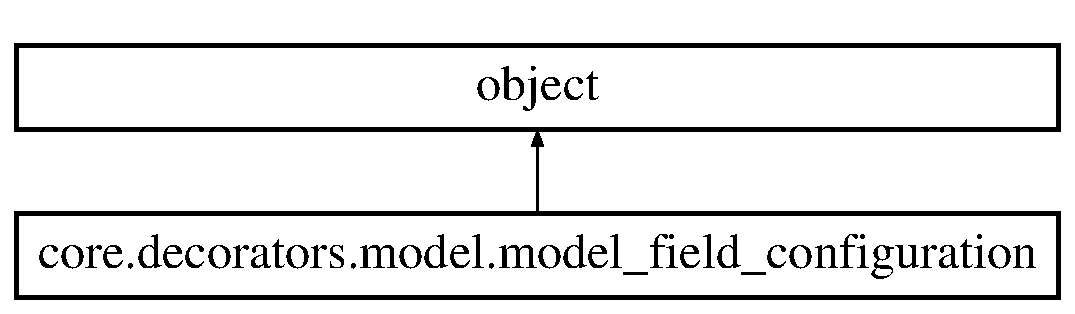
\includegraphics[height=2.000000cm]{classcore_1_1decorators_1_1model_1_1model__field__configuration}
\end{center}
\end{figure}
\subsection*{Public Member Functions}
\begin{DoxyCompactItemize}
\item 
def \hyperlink{classcore_1_1decorators_1_1model_1_1model__field__configuration_a230303617598b55606e239973dea6e84}{\-\_\-\-\_\-init\-\_\-\-\_\-}
\begin{DoxyCompactList}\small\item\em Save passed arguments. \end{DoxyCompactList}\item 
def \hyperlink{classcore_1_1decorators_1_1model_1_1model__field__configuration_afd077e96a289de0cd9fb2e350a80fee2}{\-\_\-\-\_\-call\-\_\-\-\_\-}
\begin{DoxyCompactList}\small\item\em Configure field. \end{DoxyCompactList}\end{DoxyCompactItemize}
\subsection*{Public Attributes}
\begin{DoxyCompactItemize}
\item 
\hyperlink{classcore_1_1decorators_1_1model_1_1model__field__configuration_aa400bdb842117e4d6e8b4bfcbbd20603}{name}
\item 
\hyperlink{classcore_1_1decorators_1_1model_1_1model__field__configuration_ae2ed0506f2a3f467dbc5791e61e5a459}{data}
\end{DoxyCompactItemize}


\subsection{Detailed Description}
Add extra field config to class. 


\begin{DoxyParams}{Parameters}
{\em object} & Model which will be configured \\
\hline
\end{DoxyParams}


\subsection{Constructor \& Destructor Documentation}
\hypertarget{classcore_1_1decorators_1_1model_1_1model__field__configuration_a230303617598b55606e239973dea6e84}{\index{core\-::decorators\-::model\-::model\-\_\-field\-\_\-configuration@{core\-::decorators\-::model\-::model\-\_\-field\-\_\-configuration}!\-\_\-\-\_\-init\-\_\-\-\_\-@{\-\_\-\-\_\-init\-\_\-\-\_\-}}
\index{\-\_\-\-\_\-init\-\_\-\-\_\-@{\-\_\-\-\_\-init\-\_\-\-\_\-}!core::decorators::model::model_field_configuration@{core\-::decorators\-::model\-::model\-\_\-field\-\_\-configuration}}
\subsubsection[{\-\_\-\-\_\-init\-\_\-\-\_\-}]{\setlength{\rightskip}{0pt plus 5cm}def core.\-decorators.\-model.\-model\-\_\-field\-\_\-configuration.\-\_\-\-\_\-init\-\_\-\-\_\- (
\begin{DoxyParamCaption}
\item[{}]{self, }
\item[{}]{name, }
\item[{}]{data}
\end{DoxyParamCaption}
)}}\label{classcore_1_1decorators_1_1model_1_1model__field__configuration_a230303617598b55606e239973dea6e84}


Save passed arguments. 


\begin{DoxyParams}{Parameters}
{\em name} & Field name to be extended \\
\hline
{\em data} & Field data \\
\hline
\end{DoxyParams}


\subsection{Member Function Documentation}
\hypertarget{classcore_1_1decorators_1_1model_1_1model__field__configuration_afd077e96a289de0cd9fb2e350a80fee2}{\index{core\-::decorators\-::model\-::model\-\_\-field\-\_\-configuration@{core\-::decorators\-::model\-::model\-\_\-field\-\_\-configuration}!\-\_\-\-\_\-call\-\_\-\-\_\-@{\-\_\-\-\_\-call\-\_\-\-\_\-}}
\index{\-\_\-\-\_\-call\-\_\-\-\_\-@{\-\_\-\-\_\-call\-\_\-\-\_\-}!core::decorators::model::model_field_configuration@{core\-::decorators\-::model\-::model\-\_\-field\-\_\-configuration}}
\subsubsection[{\-\_\-\-\_\-call\-\_\-\-\_\-}]{\setlength{\rightskip}{0pt plus 5cm}def core.\-decorators.\-model.\-model\-\_\-field\-\_\-configuration.\-\_\-\-\_\-call\-\_\-\-\_\- (
\begin{DoxyParamCaption}
\item[{}]{self, }
\item[{}]{cls}
\end{DoxyParamCaption}
)}}\label{classcore_1_1decorators_1_1model_1_1model__field__configuration_afd077e96a289de0cd9fb2e350a80fee2}


Configure field. 

get name of the field and widget name from arguments check if current field is title field in model


\begin{DoxyParams}{Parameters}
{\em cls} & Object we are configuring \\
\hline
\end{DoxyParams}


\subsection{Member Data Documentation}
\hypertarget{classcore_1_1decorators_1_1model_1_1model__field__configuration_ae2ed0506f2a3f467dbc5791e61e5a459}{\index{core\-::decorators\-::model\-::model\-\_\-field\-\_\-configuration@{core\-::decorators\-::model\-::model\-\_\-field\-\_\-configuration}!data@{data}}
\index{data@{data}!core::decorators::model::model_field_configuration@{core\-::decorators\-::model\-::model\-\_\-field\-\_\-configuration}}
\subsubsection[{data}]{\setlength{\rightskip}{0pt plus 5cm}core.\-decorators.\-model.\-model\-\_\-field\-\_\-configuration.\-data}}\label{classcore_1_1decorators_1_1model_1_1model__field__configuration_ae2ed0506f2a3f467dbc5791e61e5a459}
\hypertarget{classcore_1_1decorators_1_1model_1_1model__field__configuration_aa400bdb842117e4d6e8b4bfcbbd20603}{\index{core\-::decorators\-::model\-::model\-\_\-field\-\_\-configuration@{core\-::decorators\-::model\-::model\-\_\-field\-\_\-configuration}!name@{name}}
\index{name@{name}!core::decorators::model::model_field_configuration@{core\-::decorators\-::model\-::model\-\_\-field\-\_\-configuration}}
\subsubsection[{name}]{\setlength{\rightskip}{0pt plus 5cm}core.\-decorators.\-model.\-model\-\_\-field\-\_\-configuration.\-name}}\label{classcore_1_1decorators_1_1model_1_1model__field__configuration_aa400bdb842117e4d6e8b4bfcbbd20603}


The documentation for this class was generated from the following file\-:\begin{DoxyCompactItemize}
\item 
/wepo/core/decorators/\hyperlink{model_8py}{model.\-py}\end{DoxyCompactItemize}

\hypertarget{classcore_1_1decorators_1_1model_1_1model__settings}{\section{core.\-decorators.\-model.\-model\-\_\-settings Class Reference}
\label{classcore_1_1decorators_1_1model_1_1model__settings}\index{core.\-decorators.\-model.\-model\-\_\-settings@{core.\-decorators.\-model.\-model\-\_\-settings}}
}


Put model into group.  


Inheritance diagram for core.\-decorators.\-model.\-model\-\_\-settings\-:\begin{figure}[H]
\begin{center}
\leavevmode
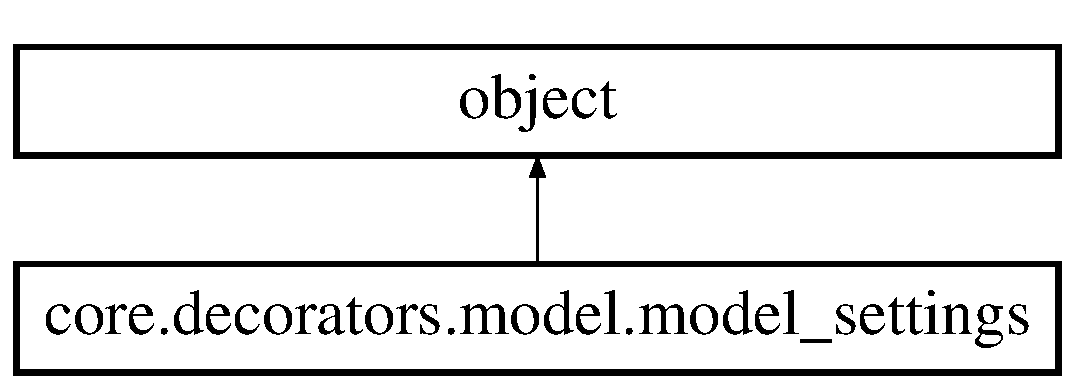
\includegraphics[height=2.000000cm]{classcore_1_1decorators_1_1model_1_1model__settings}
\end{center}
\end{figure}
\subsection*{Public Member Functions}
\begin{DoxyCompactItemize}
\item 
def \hyperlink{classcore_1_1decorators_1_1model_1_1model__settings_a4a8a0589d4e2138cb02f965f9ee0e9a6}{\-\_\-\-\_\-init\-\_\-\-\_\-}
\begin{DoxyCompactList}\small\item\em Save passed arguments. \end{DoxyCompactList}\item 
def \hyperlink{classcore_1_1decorators_1_1model_1_1model__settings_a080ab8817d1fe54b80144b77f8dfecc2}{\-\_\-\-\_\-call\-\_\-\-\_\-}
\begin{DoxyCompactList}\small\item\em Configure model group. \end{DoxyCompactList}\end{DoxyCompactItemize}
\subsection*{Public Attributes}
\begin{DoxyCompactItemize}
\item 
\hyperlink{classcore_1_1decorators_1_1model_1_1model__settings_af68f1c42015a9f9f117b36be9124c5ca}{kws}
\end{DoxyCompactItemize}


\subsection{Detailed Description}
Put model into group. 


\begin{DoxyParams}{Parameters}
{\em object} & Model which will be configured\\
\hline
\end{DoxyParams}
{\bfseries Usage} 
\begin{DoxyCode}
1 @model\_settings(group=\textcolor{stringliteral}{'group\_name'}, description=\textcolor{stringliteral}{'Model description, Lorem ipsum dolor sit amet...'})
\end{DoxyCode}
 

\subsection{Constructor \& Destructor Documentation}
\hypertarget{classcore_1_1decorators_1_1model_1_1model__settings_a4a8a0589d4e2138cb02f965f9ee0e9a6}{\index{core\-::decorators\-::model\-::model\-\_\-settings@{core\-::decorators\-::model\-::model\-\_\-settings}!\-\_\-\-\_\-init\-\_\-\-\_\-@{\-\_\-\-\_\-init\-\_\-\-\_\-}}
\index{\-\_\-\-\_\-init\-\_\-\-\_\-@{\-\_\-\-\_\-init\-\_\-\-\_\-}!core::decorators::model::model_settings@{core\-::decorators\-::model\-::model\-\_\-settings}}
\subsubsection[{\-\_\-\-\_\-init\-\_\-\-\_\-}]{\setlength{\rightskip}{0pt plus 5cm}def core.\-decorators.\-model.\-model\-\_\-settings.\-\_\-\-\_\-init\-\_\-\-\_\- (
\begin{DoxyParamCaption}
\item[{}]{self, }
\item[{}]{kws}
\end{DoxyParamCaption}
)}}\label{classcore_1_1decorators_1_1model_1_1model__settings_a4a8a0589d4e2138cb02f965f9ee0e9a6}


Save passed arguments. 


\begin{DoxyParams}{Parameters}
{\em kws} & Arguments \\
\hline
\end{DoxyParams}


\subsection{Member Function Documentation}
\hypertarget{classcore_1_1decorators_1_1model_1_1model__settings_a080ab8817d1fe54b80144b77f8dfecc2}{\index{core\-::decorators\-::model\-::model\-\_\-settings@{core\-::decorators\-::model\-::model\-\_\-settings}!\-\_\-\-\_\-call\-\_\-\-\_\-@{\-\_\-\-\_\-call\-\_\-\-\_\-}}
\index{\-\_\-\-\_\-call\-\_\-\-\_\-@{\-\_\-\-\_\-call\-\_\-\-\_\-}!core::decorators::model::model_settings@{core\-::decorators\-::model\-::model\-\_\-settings}}
\subsubsection[{\-\_\-\-\_\-call\-\_\-\-\_\-}]{\setlength{\rightskip}{0pt plus 5cm}def core.\-decorators.\-model.\-model\-\_\-settings.\-\_\-\-\_\-call\-\_\-\-\_\- (
\begin{DoxyParamCaption}
\item[{}]{self, }
\item[{}]{cls}
\end{DoxyParamCaption}
)}}\label{classcore_1_1decorators_1_1model_1_1model__settings_a080ab8817d1fe54b80144b77f8dfecc2}


Configure model group. 

set group for model


\begin{DoxyParams}{Parameters}
{\em cls} & Object we are configuring \\
\hline
\end{DoxyParams}


\subsection{Member Data Documentation}
\hypertarget{classcore_1_1decorators_1_1model_1_1model__settings_af68f1c42015a9f9f117b36be9124c5ca}{\index{core\-::decorators\-::model\-::model\-\_\-settings@{core\-::decorators\-::model\-::model\-\_\-settings}!kws@{kws}}
\index{kws@{kws}!core::decorators::model::model_settings@{core\-::decorators\-::model\-::model\-\_\-settings}}
\subsubsection[{kws}]{\setlength{\rightskip}{0pt plus 5cm}core.\-decorators.\-model.\-model\-\_\-settings.\-kws}}\label{classcore_1_1decorators_1_1model_1_1model__settings_af68f1c42015a9f9f117b36be9124c5ca}


The documentation for this class was generated from the following file\-:\begin{DoxyCompactItemize}
\item 
/wepo/core/decorators/\hyperlink{model_8py}{model.\-py}\end{DoxyCompactItemize}

\hypertarget{classcore_1_1models_1_1Page}{\section{core.\-models.\-Page Class Reference}
\label{classcore_1_1models_1_1Page}\index{core.\-models.\-Page@{core.\-models.\-Page}}
}


\hyperlink{classcore_1_1models_1_1Page}{Page}.  


Inheritance diagram for core.\-models.\-Page\-:\begin{figure}[H]
\begin{center}
\leavevmode
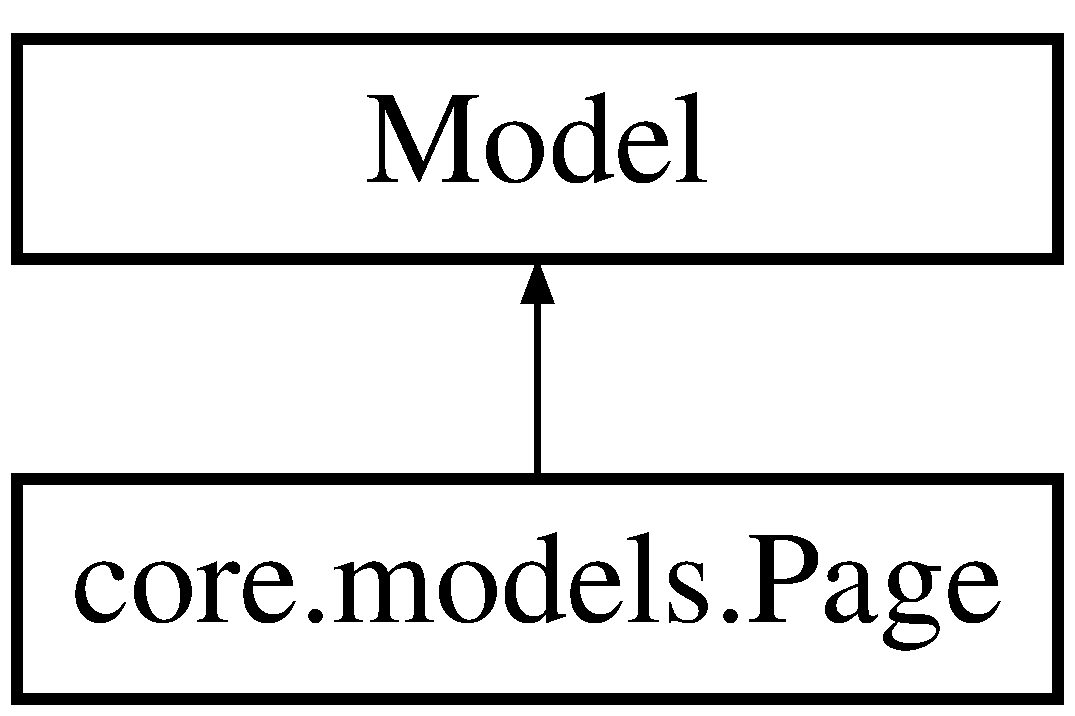
\includegraphics[height=2.000000cm]{classcore_1_1models_1_1Page}
\end{center}
\end{figure}
\subsection*{Classes}
\begin{DoxyCompactItemize}
\item 
class \hyperlink{classcore_1_1models_1_1Page_1_1Meta}{Meta}
\end{DoxyCompactItemize}
\subsection*{Public Member Functions}
\begin{DoxyCompactItemize}
\item 
def \hyperlink{classcore_1_1models_1_1Page_a1438fd9de6724c34236b99148a7f0e14}{\-\_\-\-\_\-unicode\-\_\-\-\_\-}
\item 
def \hyperlink{classcore_1_1models_1_1Page_afeb78b5c518fe105f53207535d9ddb89}{delete}
\begin{DoxyCompactList}\small\item\em Custom delete method. \end{DoxyCompactList}\item 
def \hyperlink{classcore_1_1models_1_1Page_a17d5c6f2f5fecddd39a24b4934f163fe}{save}
\begin{DoxyCompactList}\small\item\em Custom save method. \end{DoxyCompactList}\item 
def \hyperlink{classcore_1_1models_1_1Page_ae8bb1e3e592ad6187bb4ae0d959a65a4}{get\-\_\-seo}
\begin{DoxyCompactList}\small\item\em Get seo link. \end{DoxyCompactList}\end{DoxyCompactItemize}
\subsection*{Public Attributes}
\begin{DoxyCompactItemize}
\item 
\hyperlink{classcore_1_1models_1_1Page_acab3eb077ef1d77f01a48bff74c956df}{enabled}
\item 
\hyperlink{classcore_1_1models_1_1Page_a25178e4dfd9fafc8e1e6dea92ed53471}{key\-\_\-name}
\end{DoxyCompactItemize}
\subsection*{Static Public Attributes}
\begin{DoxyCompactItemize}
\item 
tuple \hyperlink{classcore_1_1models_1_1Page_a78ec187207c0e8f2c223693265a67482}{parent} = dmodels.\-Foreign\-Key('self', null=True, blank=True)
\begin{DoxyCompactList}\small\item\em Parent of the page. \end{DoxyCompactList}\item 
tuple \hyperlink{classcore_1_1models_1_1Page_a6d9d0e7d9e679e159e300f5664dc30f3}{name} = dmodels.\-Char\-Field(max\-\_\-length=64, db\-\_\-index=True)
\begin{DoxyCompactList}\small\item\em \hyperlink{classcore_1_1models_1_1Page}{Page} name. \end{DoxyCompactList}\item 
tuple \hyperlink{classcore_1_1models_1_1Page_a25178e4dfd9fafc8e1e6dea92ed53471}{key\-\_\-name} = dmodels.\-Char\-Field(max\-\_\-length=64, db\-\_\-index=True)
\begin{DoxyCompactList}\small\item\em Unique identifier of the layout. \end{DoxyCompactList}\item 
tuple \hyperlink{classcore_1_1models_1_1Page_acab3eb077ef1d77f01a48bff74c956df}{enabled} = dmodels.\-Boolean\-Field(default=True)
\begin{DoxyCompactList}\small\item\em Status if the page is enabled. \end{DoxyCompactList}\item 
tuple \hyperlink{classcore_1_1models_1_1Page_a2f5022d3c036a292307aa93776e9ef0a}{layout} = dmodels.\-Char\-Field(max\-\_\-length=255, db\-\_\-index=True)
\begin{DoxyCompactList}\small\item\em \hyperlink{classcore_1_1models_1_1Page}{Page} layout. \end{DoxyCompactList}\item 
tuple \hyperlink{classcore_1_1models_1_1Page_ac8581869cbe320c85b6be487430d23ef}{permissions} = \hyperlink{classcore_1_1fields_1_1JsonField}{Json\-Field}(null=True, blank=True)
\begin{DoxyCompactList}\small\item\em \hyperlink{classcore_1_1models_1_1Page}{Page} permissions. \end{DoxyCompactList}\item 
tuple \hyperlink{classcore_1_1models_1_1Page_a8929e212abf0bd54841eff713c431039}{blocks} = \hyperlink{classcore_1_1fields_1_1JsonField}{Json\-Field}(null=True, blank=True)
\begin{DoxyCompactList}\small\item\em \hyperlink{classcore_1_1models_1_1Page}{Page} blocks. \end{DoxyCompactList}\item 
tuple \hyperlink{classcore_1_1models_1_1Page_a2be141ff9260f87470c61991ef24d924}{assets} = \hyperlink{classcore_1_1fields_1_1JsonField}{Json\-Field}(null=True, blank=True)
\begin{DoxyCompactList}\small\item\em \hyperlink{classcore_1_1models_1_1Page}{Page} assets. \end{DoxyCompactList}\item 
int \hyperlink{classcore_1_1models_1_1Page_ad187b76ce6d3fa0e61f125da2536744e}{wepo\-\_\-counter} = 0
\end{DoxyCompactItemize}


\subsection{Detailed Description}
\hyperlink{classcore_1_1models_1_1Page}{Page}. 

\subsection{Member Function Documentation}
\hypertarget{classcore_1_1models_1_1Page_a1438fd9de6724c34236b99148a7f0e14}{\index{core\-::models\-::\-Page@{core\-::models\-::\-Page}!\-\_\-\-\_\-unicode\-\_\-\-\_\-@{\-\_\-\-\_\-unicode\-\_\-\-\_\-}}
\index{\-\_\-\-\_\-unicode\-\_\-\-\_\-@{\-\_\-\-\_\-unicode\-\_\-\-\_\-}!core::models::Page@{core\-::models\-::\-Page}}
\subsubsection[{\-\_\-\-\_\-unicode\-\_\-\-\_\-}]{\setlength{\rightskip}{0pt plus 5cm}def core.\-models.\-Page.\-\_\-\-\_\-unicode\-\_\-\-\_\- (
\begin{DoxyParamCaption}
\item[{}]{self}
\end{DoxyParamCaption}
)}}\label{classcore_1_1models_1_1Page_a1438fd9de6724c34236b99148a7f0e14}
\hypertarget{classcore_1_1models_1_1Page_afeb78b5c518fe105f53207535d9ddb89}{\index{core\-::models\-::\-Page@{core\-::models\-::\-Page}!delete@{delete}}
\index{delete@{delete}!core::models::Page@{core\-::models\-::\-Page}}
\subsubsection[{delete}]{\setlength{\rightskip}{0pt plus 5cm}def core.\-models.\-Page.\-delete (
\begin{DoxyParamCaption}
\item[{}]{self}
\end{DoxyParamCaption}
)}}\label{classcore_1_1models_1_1Page_afeb78b5c518fe105f53207535d9ddb89}


Custom delete method. 

\hypertarget{classcore_1_1models_1_1Page_ae8bb1e3e592ad6187bb4ae0d959a65a4}{\index{core\-::models\-::\-Page@{core\-::models\-::\-Page}!get\-\_\-seo@{get\-\_\-seo}}
\index{get\-\_\-seo@{get\-\_\-seo}!core::models::Page@{core\-::models\-::\-Page}}
\subsubsection[{get\-\_\-seo}]{\setlength{\rightskip}{0pt plus 5cm}def core.\-models.\-Page.\-get\-\_\-seo (
\begin{DoxyParamCaption}
\item[{}]{self}
\end{DoxyParamCaption}
)}}\label{classcore_1_1models_1_1Page_ae8bb1e3e592ad6187bb4ae0d959a65a4}


Get seo link. 

\hypertarget{classcore_1_1models_1_1Page_a17d5c6f2f5fecddd39a24b4934f163fe}{\index{core\-::models\-::\-Page@{core\-::models\-::\-Page}!save@{save}}
\index{save@{save}!core::models::Page@{core\-::models\-::\-Page}}
\subsubsection[{save}]{\setlength{\rightskip}{0pt plus 5cm}def core.\-models.\-Page.\-save (
\begin{DoxyParamCaption}
\item[{}]{self, }
\item[{}]{force\-\_\-insert = {\ttfamily False}, }
\item[{}]{force\-\_\-update = {\ttfamily False}, }
\item[{}]{using = {\ttfamily None}, }
\item[{}]{update\-\_\-fields = {\ttfamily None}}
\end{DoxyParamCaption}
)}}\label{classcore_1_1models_1_1Page_a17d5c6f2f5fecddd39a24b4934f163fe}


Custom save method. 



\subsection{Member Data Documentation}
\hypertarget{classcore_1_1models_1_1Page_a2be141ff9260f87470c61991ef24d924}{\index{core\-::models\-::\-Page@{core\-::models\-::\-Page}!assets@{assets}}
\index{assets@{assets}!core::models::Page@{core\-::models\-::\-Page}}
\subsubsection[{assets}]{\setlength{\rightskip}{0pt plus 5cm}core.\-models.\-Page.\-assets = {\bf Json\-Field}(null=True, blank=True)\hspace{0.3cm}{\ttfamily [static]}}}\label{classcore_1_1models_1_1Page_a2be141ff9260f87470c61991ef24d924}


\hyperlink{classcore_1_1models_1_1Page}{Page} assets. 

\hypertarget{classcore_1_1models_1_1Page_a8929e212abf0bd54841eff713c431039}{\index{core\-::models\-::\-Page@{core\-::models\-::\-Page}!blocks@{blocks}}
\index{blocks@{blocks}!core::models::Page@{core\-::models\-::\-Page}}
\subsubsection[{blocks}]{\setlength{\rightskip}{0pt plus 5cm}core.\-models.\-Page.\-blocks = {\bf Json\-Field}(null=True, blank=True)\hspace{0.3cm}{\ttfamily [static]}}}\label{classcore_1_1models_1_1Page_a8929e212abf0bd54841eff713c431039}


\hyperlink{classcore_1_1models_1_1Page}{Page} blocks. 

\hypertarget{classcore_1_1models_1_1Page_acab3eb077ef1d77f01a48bff74c956df}{\index{core\-::models\-::\-Page@{core\-::models\-::\-Page}!enabled@{enabled}}
\index{enabled@{enabled}!core::models::Page@{core\-::models\-::\-Page}}
\subsubsection[{enabled}]{\setlength{\rightskip}{0pt plus 5cm}core.\-models.\-Page.\-enabled = dmodels.\-Boolean\-Field(default=True)\hspace{0.3cm}{\ttfamily [static]}}}\label{classcore_1_1models_1_1Page_acab3eb077ef1d77f01a48bff74c956df}


Status if the page is enabled. 

\hypertarget{classcore_1_1models_1_1Page_acab3eb077ef1d77f01a48bff74c956df}{\index{core\-::models\-::\-Page@{core\-::models\-::\-Page}!enabled@{enabled}}
\index{enabled@{enabled}!core::models::Page@{core\-::models\-::\-Page}}
\subsubsection[{enabled}]{\setlength{\rightskip}{0pt plus 5cm}core.\-models.\-Page.\-enabled}}\label{classcore_1_1models_1_1Page_acab3eb077ef1d77f01a48bff74c956df}
\hypertarget{classcore_1_1models_1_1Page_a25178e4dfd9fafc8e1e6dea92ed53471}{\index{core\-::models\-::\-Page@{core\-::models\-::\-Page}!key\-\_\-name@{key\-\_\-name}}
\index{key\-\_\-name@{key\-\_\-name}!core::models::Page@{core\-::models\-::\-Page}}
\subsubsection[{key\-\_\-name}]{\setlength{\rightskip}{0pt plus 5cm}core.\-models.\-Page.\-key\-\_\-name = dmodels.\-Char\-Field(max\-\_\-length=64, db\-\_\-index=True)\hspace{0.3cm}{\ttfamily [static]}}}\label{classcore_1_1models_1_1Page_a25178e4dfd9fafc8e1e6dea92ed53471}


Unique identifier of the layout. 

\hypertarget{classcore_1_1models_1_1Page_a25178e4dfd9fafc8e1e6dea92ed53471}{\index{core\-::models\-::\-Page@{core\-::models\-::\-Page}!key\-\_\-name@{key\-\_\-name}}
\index{key\-\_\-name@{key\-\_\-name}!core::models::Page@{core\-::models\-::\-Page}}
\subsubsection[{key\-\_\-name}]{\setlength{\rightskip}{0pt plus 5cm}core.\-models.\-Page.\-key\-\_\-name}}\label{classcore_1_1models_1_1Page_a25178e4dfd9fafc8e1e6dea92ed53471}
\hypertarget{classcore_1_1models_1_1Page_a2f5022d3c036a292307aa93776e9ef0a}{\index{core\-::models\-::\-Page@{core\-::models\-::\-Page}!layout@{layout}}
\index{layout@{layout}!core::models::Page@{core\-::models\-::\-Page}}
\subsubsection[{layout}]{\setlength{\rightskip}{0pt plus 5cm}core.\-models.\-Page.\-layout = dmodels.\-Char\-Field(max\-\_\-length=255, db\-\_\-index=True)\hspace{0.3cm}{\ttfamily [static]}}}\label{classcore_1_1models_1_1Page_a2f5022d3c036a292307aa93776e9ef0a}


\hyperlink{classcore_1_1models_1_1Page}{Page} layout. 

\hypertarget{classcore_1_1models_1_1Page_a6d9d0e7d9e679e159e300f5664dc30f3}{\index{core\-::models\-::\-Page@{core\-::models\-::\-Page}!name@{name}}
\index{name@{name}!core::models::Page@{core\-::models\-::\-Page}}
\subsubsection[{name}]{\setlength{\rightskip}{0pt plus 5cm}core.\-models.\-Page.\-name = dmodels.\-Char\-Field(max\-\_\-length=64, db\-\_\-index=True)\hspace{0.3cm}{\ttfamily [static]}}}\label{classcore_1_1models_1_1Page_a6d9d0e7d9e679e159e300f5664dc30f3}


\hyperlink{classcore_1_1models_1_1Page}{Page} name. 

\hypertarget{classcore_1_1models_1_1Page_a78ec187207c0e8f2c223693265a67482}{\index{core\-::models\-::\-Page@{core\-::models\-::\-Page}!parent@{parent}}
\index{parent@{parent}!core::models::Page@{core\-::models\-::\-Page}}
\subsubsection[{parent}]{\setlength{\rightskip}{0pt plus 5cm}core.\-models.\-Page.\-parent = dmodels.\-Foreign\-Key('self', null=True, blank=True)\hspace{0.3cm}{\ttfamily [static]}}}\label{classcore_1_1models_1_1Page_a78ec187207c0e8f2c223693265a67482}


Parent of the page. 

\hypertarget{classcore_1_1models_1_1Page_ac8581869cbe320c85b6be487430d23ef}{\index{core\-::models\-::\-Page@{core\-::models\-::\-Page}!permissions@{permissions}}
\index{permissions@{permissions}!core::models::Page@{core\-::models\-::\-Page}}
\subsubsection[{permissions}]{\setlength{\rightskip}{0pt plus 5cm}core.\-models.\-Page.\-permissions = {\bf Json\-Field}(null=True, blank=True)\hspace{0.3cm}{\ttfamily [static]}}}\label{classcore_1_1models_1_1Page_ac8581869cbe320c85b6be487430d23ef}


\hyperlink{classcore_1_1models_1_1Page}{Page} permissions. 

\hypertarget{classcore_1_1models_1_1Page_ad187b76ce6d3fa0e61f125da2536744e}{\index{core\-::models\-::\-Page@{core\-::models\-::\-Page}!wepo\-\_\-counter@{wepo\-\_\-counter}}
\index{wepo\-\_\-counter@{wepo\-\_\-counter}!core::models::Page@{core\-::models\-::\-Page}}
\subsubsection[{wepo\-\_\-counter}]{\setlength{\rightskip}{0pt plus 5cm}int core.\-models.\-Page.\-wepo\-\_\-counter = 0\hspace{0.3cm}{\ttfamily [static]}}}\label{classcore_1_1models_1_1Page_ad187b76ce6d3fa0e61f125da2536744e}


The documentation for this class was generated from the following file\-:\begin{DoxyCompactItemize}
\item 
/wepo/core/\hyperlink{models_8py}{models.\-py}\end{DoxyCompactItemize}

\hypertarget{classcore_1_1templatetags_1_1core__tags_1_1PermissionNode}{\section{core.\-templatetags.\-core\-\_\-tags.\-Permission\-Node Class Reference}
\label{classcore_1_1templatetags_1_1core__tags_1_1PermissionNode}\index{core.\-templatetags.\-core\-\_\-tags.\-Permission\-Node@{core.\-templatetags.\-core\-\_\-tags.\-Permission\-Node}}
}


Permission tag helper class to render tokens.  


Inheritance diagram for core.\-templatetags.\-core\-\_\-tags.\-Permission\-Node\-:\begin{figure}[H]
\begin{center}
\leavevmode
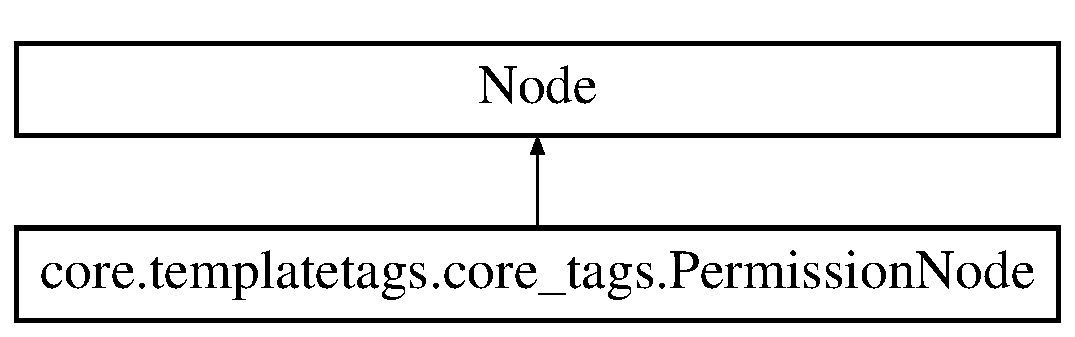
\includegraphics[height=2.000000cm]{classcore_1_1templatetags_1_1core__tags_1_1PermissionNode}
\end{center}
\end{figure}
\subsection*{Public Member Functions}
\begin{DoxyCompactItemize}
\item 
def \hyperlink{classcore_1_1templatetags_1_1core__tags_1_1PermissionNode_a42fb743243a3a57c033abb71e0b5b975}{\-\_\-\-\_\-init\-\_\-\-\_\-}
\item 
def \hyperlink{classcore_1_1templatetags_1_1core__tags_1_1PermissionNode_adda756edbbf52cf0949d91430128495a}{render}
\end{DoxyCompactItemize}
\subsection*{Public Attributes}
\begin{DoxyCompactItemize}
\item 
\hyperlink{classcore_1_1templatetags_1_1core__tags_1_1PermissionNode_a8f264cfa76767dba610e4a0b930a69e3}{permissions}
\item 
\hyperlink{classcore_1_1templatetags_1_1core__tags_1_1PermissionNode_a702425b36ea18844eee836560b3c3215}{nodelist\-\_\-permission}
\item 
\hyperlink{classcore_1_1templatetags_1_1core__tags_1_1PermissionNode_ab3b7efaa62b6ac8b71cc33ae49356b19}{nodelist\-\_\-nopermission}
\end{DoxyCompactItemize}


\subsection{Detailed Description}
Permission tag helper class to render tokens. 

\subsection{Constructor \& Destructor Documentation}
\hypertarget{classcore_1_1templatetags_1_1core__tags_1_1PermissionNode_a42fb743243a3a57c033abb71e0b5b975}{\index{core\-::templatetags\-::core\-\_\-tags\-::\-Permission\-Node@{core\-::templatetags\-::core\-\_\-tags\-::\-Permission\-Node}!\-\_\-\-\_\-init\-\_\-\-\_\-@{\-\_\-\-\_\-init\-\_\-\-\_\-}}
\index{\-\_\-\-\_\-init\-\_\-\-\_\-@{\-\_\-\-\_\-init\-\_\-\-\_\-}!core::templatetags::core_tags::PermissionNode@{core\-::templatetags\-::core\-\_\-tags\-::\-Permission\-Node}}
\subsubsection[{\-\_\-\-\_\-init\-\_\-\-\_\-}]{\setlength{\rightskip}{0pt plus 5cm}def core.\-templatetags.\-core\-\_\-tags.\-Permission\-Node.\-\_\-\-\_\-init\-\_\-\-\_\- (
\begin{DoxyParamCaption}
\item[{}]{self, }
\item[{}]{permissions, }
\item[{}]{nodelist\-\_\-permission, }
\item[{}]{nodelist\-\_\-nopermission}
\end{DoxyParamCaption}
)}}\label{classcore_1_1templatetags_1_1core__tags_1_1PermissionNode_a42fb743243a3a57c033abb71e0b5b975}


\subsection{Member Function Documentation}
\hypertarget{classcore_1_1templatetags_1_1core__tags_1_1PermissionNode_adda756edbbf52cf0949d91430128495a}{\index{core\-::templatetags\-::core\-\_\-tags\-::\-Permission\-Node@{core\-::templatetags\-::core\-\_\-tags\-::\-Permission\-Node}!render@{render}}
\index{render@{render}!core::templatetags::core_tags::PermissionNode@{core\-::templatetags\-::core\-\_\-tags\-::\-Permission\-Node}}
\subsubsection[{render}]{\setlength{\rightskip}{0pt plus 5cm}def core.\-templatetags.\-core\-\_\-tags.\-Permission\-Node.\-render (
\begin{DoxyParamCaption}
\item[{}]{self, }
\item[{}]{context}
\end{DoxyParamCaption}
)}}\label{classcore_1_1templatetags_1_1core__tags_1_1PermissionNode_adda756edbbf52cf0949d91430128495a}


\subsection{Member Data Documentation}
\hypertarget{classcore_1_1templatetags_1_1core__tags_1_1PermissionNode_ab3b7efaa62b6ac8b71cc33ae49356b19}{\index{core\-::templatetags\-::core\-\_\-tags\-::\-Permission\-Node@{core\-::templatetags\-::core\-\_\-tags\-::\-Permission\-Node}!nodelist\-\_\-nopermission@{nodelist\-\_\-nopermission}}
\index{nodelist\-\_\-nopermission@{nodelist\-\_\-nopermission}!core::templatetags::core_tags::PermissionNode@{core\-::templatetags\-::core\-\_\-tags\-::\-Permission\-Node}}
\subsubsection[{nodelist\-\_\-nopermission}]{\setlength{\rightskip}{0pt plus 5cm}core.\-templatetags.\-core\-\_\-tags.\-Permission\-Node.\-nodelist\-\_\-nopermission}}\label{classcore_1_1templatetags_1_1core__tags_1_1PermissionNode_ab3b7efaa62b6ac8b71cc33ae49356b19}
\hypertarget{classcore_1_1templatetags_1_1core__tags_1_1PermissionNode_a702425b36ea18844eee836560b3c3215}{\index{core\-::templatetags\-::core\-\_\-tags\-::\-Permission\-Node@{core\-::templatetags\-::core\-\_\-tags\-::\-Permission\-Node}!nodelist\-\_\-permission@{nodelist\-\_\-permission}}
\index{nodelist\-\_\-permission@{nodelist\-\_\-permission}!core::templatetags::core_tags::PermissionNode@{core\-::templatetags\-::core\-\_\-tags\-::\-Permission\-Node}}
\subsubsection[{nodelist\-\_\-permission}]{\setlength{\rightskip}{0pt plus 5cm}core.\-templatetags.\-core\-\_\-tags.\-Permission\-Node.\-nodelist\-\_\-permission}}\label{classcore_1_1templatetags_1_1core__tags_1_1PermissionNode_a702425b36ea18844eee836560b3c3215}
\hypertarget{classcore_1_1templatetags_1_1core__tags_1_1PermissionNode_a8f264cfa76767dba610e4a0b930a69e3}{\index{core\-::templatetags\-::core\-\_\-tags\-::\-Permission\-Node@{core\-::templatetags\-::core\-\_\-tags\-::\-Permission\-Node}!permissions@{permissions}}
\index{permissions@{permissions}!core::templatetags::core_tags::PermissionNode@{core\-::templatetags\-::core\-\_\-tags\-::\-Permission\-Node}}
\subsubsection[{permissions}]{\setlength{\rightskip}{0pt plus 5cm}core.\-templatetags.\-core\-\_\-tags.\-Permission\-Node.\-permissions}}\label{classcore_1_1templatetags_1_1core__tags_1_1PermissionNode_a8f264cfa76767dba610e4a0b930a69e3}


The documentation for this class was generated from the following file\-:\begin{DoxyCompactItemize}
\item 
/wepo/core/templatetags/\hyperlink{core__tags_8py}{core\-\_\-tags.\-py}\end{DoxyCompactItemize}

\hypertarget{classcore_1_1json__cache_1_1Pickler}{\section{core.\-json\-\_\-cache.\-Pickler Class Reference}
\label{classcore_1_1json__cache_1_1Pickler}\index{core.\-json\-\_\-cache.\-Pickler@{core.\-json\-\_\-cache.\-Pickler}}
}
Inheritance diagram for core.\-json\-\_\-cache.\-Pickler\-:\begin{figure}[H]
\begin{center}
\leavevmode
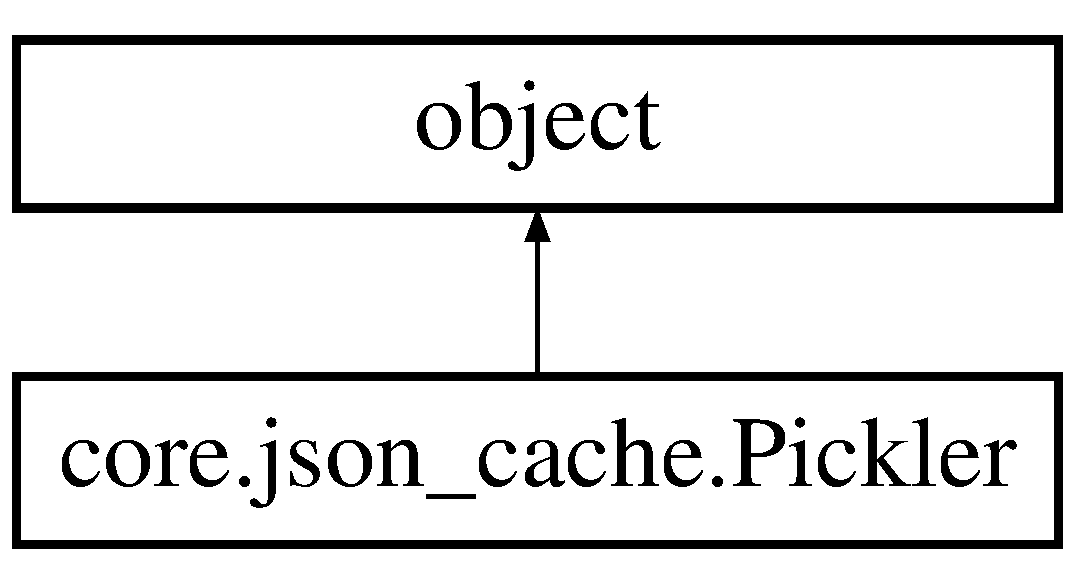
\includegraphics[height=2.000000cm]{classcore_1_1json__cache_1_1Pickler}
\end{center}
\end{figure}
\subsection*{Public Member Functions}
\begin{DoxyCompactItemize}
\item 
def \hyperlink{classcore_1_1json__cache_1_1Pickler_ad351b16c64995e93593d9bbeefbc9b51}{\-\_\-\-\_\-init\-\_\-\-\_\-}
\item 
def \hyperlink{classcore_1_1json__cache_1_1Pickler_add92d9551f473260075ccf605d2c5b0e}{dump}
\end{DoxyCompactItemize}
\subsection*{Public Attributes}
\begin{DoxyCompactItemize}
\item 
\hyperlink{classcore_1_1json__cache_1_1Pickler_a3597719d57409ead6e111dab46bbefbd}{fp}
\end{DoxyCompactItemize}


\subsection{Constructor \& Destructor Documentation}
\hypertarget{classcore_1_1json__cache_1_1Pickler_ad351b16c64995e93593d9bbeefbc9b51}{\index{core\-::json\-\_\-cache\-::\-Pickler@{core\-::json\-\_\-cache\-::\-Pickler}!\-\_\-\-\_\-init\-\_\-\-\_\-@{\-\_\-\-\_\-init\-\_\-\-\_\-}}
\index{\-\_\-\-\_\-init\-\_\-\-\_\-@{\-\_\-\-\_\-init\-\_\-\-\_\-}!core::json_cache::Pickler@{core\-::json\-\_\-cache\-::\-Pickler}}
\subsubsection[{\-\_\-\-\_\-init\-\_\-\-\_\-}]{\setlength{\rightskip}{0pt plus 5cm}def core.\-json\-\_\-cache.\-Pickler.\-\_\-\-\_\-init\-\_\-\-\_\- (
\begin{DoxyParamCaption}
\item[{}]{self, }
\item[{}]{fp, }
\item[{}]{args, }
\item[{}]{argv}
\end{DoxyParamCaption}
)}}\label{classcore_1_1json__cache_1_1Pickler_ad351b16c64995e93593d9bbeefbc9b51}


\subsection{Member Function Documentation}
\hypertarget{classcore_1_1json__cache_1_1Pickler_add92d9551f473260075ccf605d2c5b0e}{\index{core\-::json\-\_\-cache\-::\-Pickler@{core\-::json\-\_\-cache\-::\-Pickler}!dump@{dump}}
\index{dump@{dump}!core::json_cache::Pickler@{core\-::json\-\_\-cache\-::\-Pickler}}
\subsubsection[{dump}]{\setlength{\rightskip}{0pt plus 5cm}def core.\-json\-\_\-cache.\-Pickler.\-dump (
\begin{DoxyParamCaption}
\item[{}]{self, }
\item[{}]{obj}
\end{DoxyParamCaption}
)}}\label{classcore_1_1json__cache_1_1Pickler_add92d9551f473260075ccf605d2c5b0e}


\subsection{Member Data Documentation}
\hypertarget{classcore_1_1json__cache_1_1Pickler_a3597719d57409ead6e111dab46bbefbd}{\index{core\-::json\-\_\-cache\-::\-Pickler@{core\-::json\-\_\-cache\-::\-Pickler}!fp@{fp}}
\index{fp@{fp}!core::json_cache::Pickler@{core\-::json\-\_\-cache\-::\-Pickler}}
\subsubsection[{fp}]{\setlength{\rightskip}{0pt plus 5cm}core.\-json\-\_\-cache.\-Pickler.\-fp}}\label{classcore_1_1json__cache_1_1Pickler_a3597719d57409ead6e111dab46bbefbd}


The documentation for this class was generated from the following file\-:\begin{DoxyCompactItemize}
\item 
/wepo/core/\hyperlink{json__cache_8py}{json\-\_\-cache.\-py}\end{DoxyCompactItemize}

\hypertarget{classcore_1_1templatetags_1_1core__tags_1_1RequestNode}{\section{core.\-templatetags.\-core\-\_\-tags.\-Request\-Node Class Reference}
\label{classcore_1_1templatetags_1_1core__tags_1_1RequestNode}\index{core.\-templatetags.\-core\-\_\-tags.\-Request\-Node@{core.\-templatetags.\-core\-\_\-tags.\-Request\-Node}}
}
Inheritance diagram for core.\-templatetags.\-core\-\_\-tags.\-Request\-Node\-:\begin{figure}[H]
\begin{center}
\leavevmode
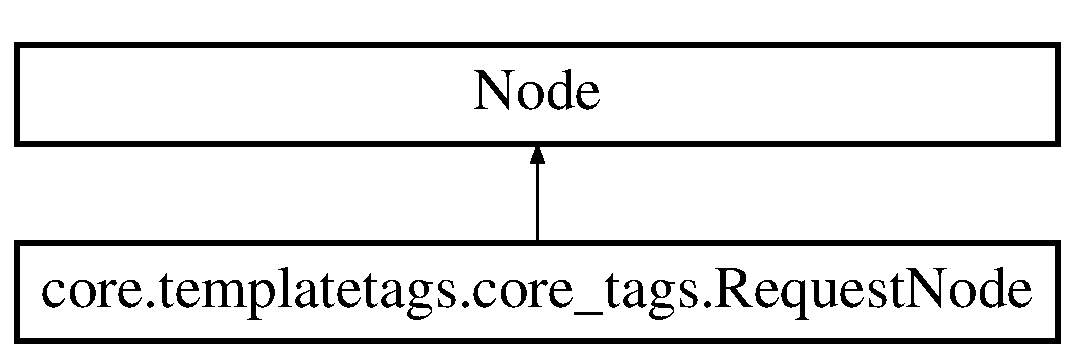
\includegraphics[height=2.000000cm]{classcore_1_1templatetags_1_1core__tags_1_1RequestNode}
\end{center}
\end{figure}
\subsection*{Public Member Functions}
\begin{DoxyCompactItemize}
\item 
def \hyperlink{classcore_1_1templatetags_1_1core__tags_1_1RequestNode_ac3376ab8191e796d84f7a498f481d165}{\-\_\-\-\_\-init\-\_\-\-\_\-}
\item 
def \hyperlink{classcore_1_1templatetags_1_1core__tags_1_1RequestNode_a2098171f856d3a327bccc591477692fc}{render}
\end{DoxyCompactItemize}
\subsection*{Public Attributes}
\begin{DoxyCompactItemize}
\item 
\hyperlink{classcore_1_1templatetags_1_1core__tags_1_1RequestNode_aa9704d30f35d2b11b9e2d11576ec2406}{nodelist\-\_\-field}
\end{DoxyCompactItemize}


\subsection{Constructor \& Destructor Documentation}
\hypertarget{classcore_1_1templatetags_1_1core__tags_1_1RequestNode_ac3376ab8191e796d84f7a498f481d165}{\index{core\-::templatetags\-::core\-\_\-tags\-::\-Request\-Node@{core\-::templatetags\-::core\-\_\-tags\-::\-Request\-Node}!\-\_\-\-\_\-init\-\_\-\-\_\-@{\-\_\-\-\_\-init\-\_\-\-\_\-}}
\index{\-\_\-\-\_\-init\-\_\-\-\_\-@{\-\_\-\-\_\-init\-\_\-\-\_\-}!core::templatetags::core_tags::RequestNode@{core\-::templatetags\-::core\-\_\-tags\-::\-Request\-Node}}
\subsubsection[{\-\_\-\-\_\-init\-\_\-\-\_\-}]{\setlength{\rightskip}{0pt plus 5cm}def core.\-templatetags.\-core\-\_\-tags.\-Request\-Node.\-\_\-\-\_\-init\-\_\-\-\_\- (
\begin{DoxyParamCaption}
\item[{}]{self, }
\item[{}]{nodelist\-\_\-field}
\end{DoxyParamCaption}
)}}\label{classcore_1_1templatetags_1_1core__tags_1_1RequestNode_ac3376ab8191e796d84f7a498f481d165}


\subsection{Member Function Documentation}
\hypertarget{classcore_1_1templatetags_1_1core__tags_1_1RequestNode_a2098171f856d3a327bccc591477692fc}{\index{core\-::templatetags\-::core\-\_\-tags\-::\-Request\-Node@{core\-::templatetags\-::core\-\_\-tags\-::\-Request\-Node}!render@{render}}
\index{render@{render}!core::templatetags::core_tags::RequestNode@{core\-::templatetags\-::core\-\_\-tags\-::\-Request\-Node}}
\subsubsection[{render}]{\setlength{\rightskip}{0pt plus 5cm}def core.\-templatetags.\-core\-\_\-tags.\-Request\-Node.\-render (
\begin{DoxyParamCaption}
\item[{}]{self, }
\item[{}]{context}
\end{DoxyParamCaption}
)}}\label{classcore_1_1templatetags_1_1core__tags_1_1RequestNode_a2098171f856d3a327bccc591477692fc}


\subsection{Member Data Documentation}
\hypertarget{classcore_1_1templatetags_1_1core__tags_1_1RequestNode_aa9704d30f35d2b11b9e2d11576ec2406}{\index{core\-::templatetags\-::core\-\_\-tags\-::\-Request\-Node@{core\-::templatetags\-::core\-\_\-tags\-::\-Request\-Node}!nodelist\-\_\-field@{nodelist\-\_\-field}}
\index{nodelist\-\_\-field@{nodelist\-\_\-field}!core::templatetags::core_tags::RequestNode@{core\-::templatetags\-::core\-\_\-tags\-::\-Request\-Node}}
\subsubsection[{nodelist\-\_\-field}]{\setlength{\rightskip}{0pt plus 5cm}core.\-templatetags.\-core\-\_\-tags.\-Request\-Node.\-nodelist\-\_\-field}}\label{classcore_1_1templatetags_1_1core__tags_1_1RequestNode_aa9704d30f35d2b11b9e2d11576ec2406}


The documentation for this class was generated from the following file\-:\begin{DoxyCompactItemize}
\item 
/wepo/core/templatetags/\hyperlink{core__tags_8py}{core\-\_\-tags.\-py}\end{DoxyCompactItemize}

\hypertarget{classcore_1_1templatetags_1_1core__tags_1_1SectionsNode}{\section{core.\-templatetags.\-core\-\_\-tags.\-Sections\-Node Class Reference}
\label{classcore_1_1templatetags_1_1core__tags_1_1SectionsNode}\index{core.\-templatetags.\-core\-\_\-tags.\-Sections\-Node@{core.\-templatetags.\-core\-\_\-tags.\-Sections\-Node}}
}
Inheritance diagram for core.\-templatetags.\-core\-\_\-tags.\-Sections\-Node\-:\begin{figure}[H]
\begin{center}
\leavevmode
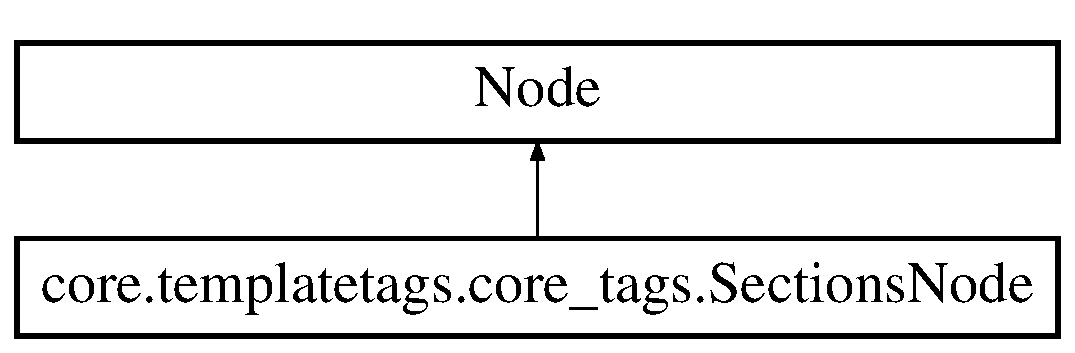
\includegraphics[height=2.000000cm]{classcore_1_1templatetags_1_1core__tags_1_1SectionsNode}
\end{center}
\end{figure}
\subsection*{Public Member Functions}
\begin{DoxyCompactItemize}
\item 
def \hyperlink{classcore_1_1templatetags_1_1core__tags_1_1SectionsNode_a715af6c362732ace4353c5194eba6872}{\-\_\-\-\_\-init\-\_\-\-\_\-}
\item 
def \hyperlink{classcore_1_1templatetags_1_1core__tags_1_1SectionsNode_a802e2701690f2a4e6a27dee4964e23d9}{render}
\end{DoxyCompactItemize}
\subsection*{Public Attributes}
\begin{DoxyCompactItemize}
\item 
\hyperlink{classcore_1_1templatetags_1_1core__tags_1_1SectionsNode_a03036dd42e3c41e6e861188adb81ea57}{section}
\item 
\hyperlink{classcore_1_1templatetags_1_1core__tags_1_1SectionsNode_a1f38a0010f2b78a29cf04ba071f4edec}{page}
\item 
\hyperlink{classcore_1_1templatetags_1_1core__tags_1_1SectionsNode_a5271892d91e1feed9afae8efd635e413}{output\-\_\-var}
\item 
\hyperlink{classcore_1_1templatetags_1_1core__tags_1_1SectionsNode_ae4ce1976f4351eacbed3ae92631dff1f}{nodelist\-\_\-field}
\end{DoxyCompactItemize}


\subsection{Constructor \& Destructor Documentation}
\hypertarget{classcore_1_1templatetags_1_1core__tags_1_1SectionsNode_a715af6c362732ace4353c5194eba6872}{\index{core\-::templatetags\-::core\-\_\-tags\-::\-Sections\-Node@{core\-::templatetags\-::core\-\_\-tags\-::\-Sections\-Node}!\-\_\-\-\_\-init\-\_\-\-\_\-@{\-\_\-\-\_\-init\-\_\-\-\_\-}}
\index{\-\_\-\-\_\-init\-\_\-\-\_\-@{\-\_\-\-\_\-init\-\_\-\-\_\-}!core::templatetags::core_tags::SectionsNode@{core\-::templatetags\-::core\-\_\-tags\-::\-Sections\-Node}}
\subsubsection[{\-\_\-\-\_\-init\-\_\-\-\_\-}]{\setlength{\rightskip}{0pt plus 5cm}def core.\-templatetags.\-core\-\_\-tags.\-Sections\-Node.\-\_\-\-\_\-init\-\_\-\-\_\- (
\begin{DoxyParamCaption}
\item[{}]{self, }
\item[{}]{section, }
\item[{}]{page, }
\item[{}]{output\-\_\-var, }
\item[{}]{nodelist\-\_\-field}
\end{DoxyParamCaption}
)}}\label{classcore_1_1templatetags_1_1core__tags_1_1SectionsNode_a715af6c362732ace4353c5194eba6872}


\subsection{Member Function Documentation}
\hypertarget{classcore_1_1templatetags_1_1core__tags_1_1SectionsNode_a802e2701690f2a4e6a27dee4964e23d9}{\index{core\-::templatetags\-::core\-\_\-tags\-::\-Sections\-Node@{core\-::templatetags\-::core\-\_\-tags\-::\-Sections\-Node}!render@{render}}
\index{render@{render}!core::templatetags::core_tags::SectionsNode@{core\-::templatetags\-::core\-\_\-tags\-::\-Sections\-Node}}
\subsubsection[{render}]{\setlength{\rightskip}{0pt plus 5cm}def core.\-templatetags.\-core\-\_\-tags.\-Sections\-Node.\-render (
\begin{DoxyParamCaption}
\item[{}]{self, }
\item[{}]{context}
\end{DoxyParamCaption}
)}}\label{classcore_1_1templatetags_1_1core__tags_1_1SectionsNode_a802e2701690f2a4e6a27dee4964e23d9}


\subsection{Member Data Documentation}
\hypertarget{classcore_1_1templatetags_1_1core__tags_1_1SectionsNode_ae4ce1976f4351eacbed3ae92631dff1f}{\index{core\-::templatetags\-::core\-\_\-tags\-::\-Sections\-Node@{core\-::templatetags\-::core\-\_\-tags\-::\-Sections\-Node}!nodelist\-\_\-field@{nodelist\-\_\-field}}
\index{nodelist\-\_\-field@{nodelist\-\_\-field}!core::templatetags::core_tags::SectionsNode@{core\-::templatetags\-::core\-\_\-tags\-::\-Sections\-Node}}
\subsubsection[{nodelist\-\_\-field}]{\setlength{\rightskip}{0pt plus 5cm}core.\-templatetags.\-core\-\_\-tags.\-Sections\-Node.\-nodelist\-\_\-field}}\label{classcore_1_1templatetags_1_1core__tags_1_1SectionsNode_ae4ce1976f4351eacbed3ae92631dff1f}
\hypertarget{classcore_1_1templatetags_1_1core__tags_1_1SectionsNode_a5271892d91e1feed9afae8efd635e413}{\index{core\-::templatetags\-::core\-\_\-tags\-::\-Sections\-Node@{core\-::templatetags\-::core\-\_\-tags\-::\-Sections\-Node}!output\-\_\-var@{output\-\_\-var}}
\index{output\-\_\-var@{output\-\_\-var}!core::templatetags::core_tags::SectionsNode@{core\-::templatetags\-::core\-\_\-tags\-::\-Sections\-Node}}
\subsubsection[{output\-\_\-var}]{\setlength{\rightskip}{0pt plus 5cm}core.\-templatetags.\-core\-\_\-tags.\-Sections\-Node.\-output\-\_\-var}}\label{classcore_1_1templatetags_1_1core__tags_1_1SectionsNode_a5271892d91e1feed9afae8efd635e413}
\hypertarget{classcore_1_1templatetags_1_1core__tags_1_1SectionsNode_a1f38a0010f2b78a29cf04ba071f4edec}{\index{core\-::templatetags\-::core\-\_\-tags\-::\-Sections\-Node@{core\-::templatetags\-::core\-\_\-tags\-::\-Sections\-Node}!page@{page}}
\index{page@{page}!core::templatetags::core_tags::SectionsNode@{core\-::templatetags\-::core\-\_\-tags\-::\-Sections\-Node}}
\subsubsection[{page}]{\setlength{\rightskip}{0pt plus 5cm}core.\-templatetags.\-core\-\_\-tags.\-Sections\-Node.\-page}}\label{classcore_1_1templatetags_1_1core__tags_1_1SectionsNode_a1f38a0010f2b78a29cf04ba071f4edec}
\hypertarget{classcore_1_1templatetags_1_1core__tags_1_1SectionsNode_a03036dd42e3c41e6e861188adb81ea57}{\index{core\-::templatetags\-::core\-\_\-tags\-::\-Sections\-Node@{core\-::templatetags\-::core\-\_\-tags\-::\-Sections\-Node}!section@{section}}
\index{section@{section}!core::templatetags::core_tags::SectionsNode@{core\-::templatetags\-::core\-\_\-tags\-::\-Sections\-Node}}
\subsubsection[{section}]{\setlength{\rightskip}{0pt plus 5cm}core.\-templatetags.\-core\-\_\-tags.\-Sections\-Node.\-section}}\label{classcore_1_1templatetags_1_1core__tags_1_1SectionsNode_a03036dd42e3c41e6e861188adb81ea57}


The documentation for this class was generated from the following file\-:\begin{DoxyCompactItemize}
\item 
/wepo/core/templatetags/\hyperlink{core__tags_8py}{core\-\_\-tags.\-py}\end{DoxyCompactItemize}

\hypertarget{classcore_1_1models_1_1Seo}{\section{core.\-models.\-Seo Class Reference}
\label{classcore_1_1models_1_1Seo}\index{core.\-models.\-Seo@{core.\-models.\-Seo}}
}


\hyperlink{classcore_1_1models_1_1Seo}{Seo}.  


Inheritance diagram for core.\-models.\-Seo\-:\begin{figure}[H]
\begin{center}
\leavevmode
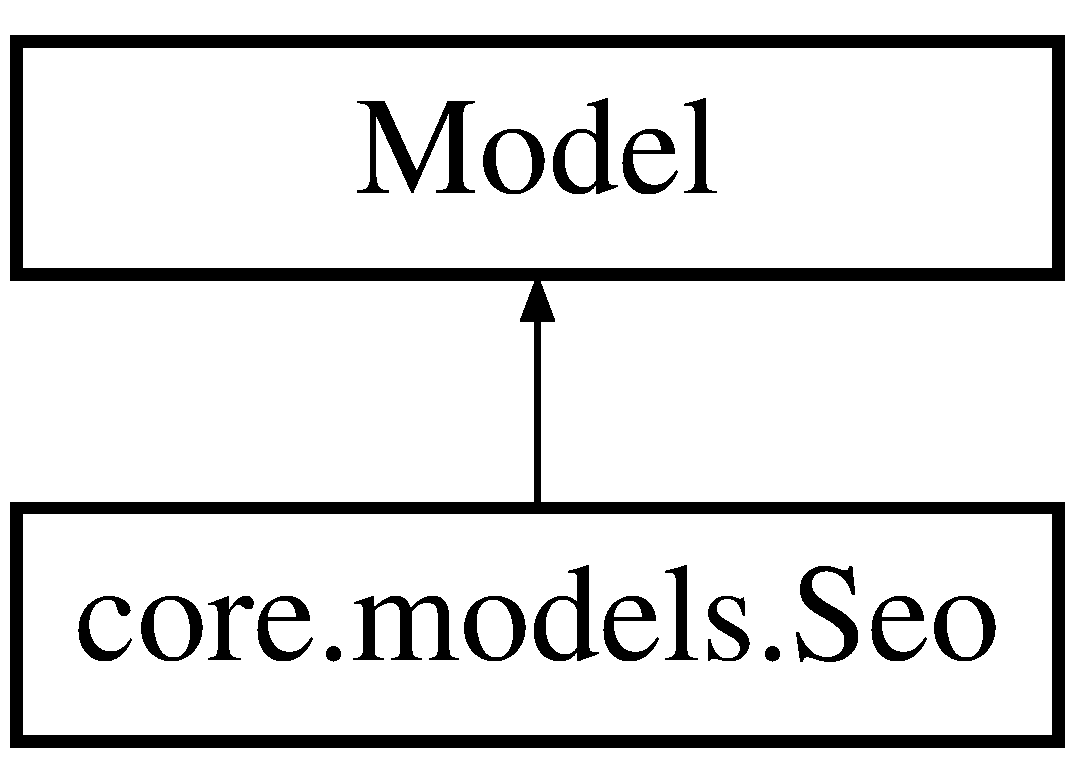
\includegraphics[height=2.000000cm]{classcore_1_1models_1_1Seo}
\end{center}
\end{figure}
\subsection*{Classes}
\begin{DoxyCompactItemize}
\item 
class \hyperlink{classcore_1_1models_1_1Seo_1_1Meta}{Meta}
\end{DoxyCompactItemize}
\subsection*{Public Member Functions}
\begin{DoxyCompactItemize}
\item 
def \hyperlink{classcore_1_1models_1_1Seo_abcdc25916c3a122583536783a570b929}{\-\_\-\-\_\-unicode\-\_\-\-\_\-}
\item 
def \hyperlink{classcore_1_1models_1_1Seo_a34873176512334dc1aadb3eaceff0017}{delete}
\begin{DoxyCompactList}\small\item\em Custom delete method. \end{DoxyCompactList}\item 
def \hyperlink{classcore_1_1models_1_1Seo_a9851406bdaf723e7ad3df70251eafb93}{save}
\begin{DoxyCompactList}\small\item\em Custom save method. \end{DoxyCompactList}\item 
def \hyperlink{classcore_1_1models_1_1Seo_a1eeec2b20f1ef7ff477688c6d954ffd9}{get\-\_\-model\-\_\-seo}
\begin{DoxyCompactList}\small\item\em Get seo for model. \end{DoxyCompactList}\item 
def \hyperlink{classcore_1_1models_1_1Seo_aec1160ede01bc3550806a3b028455289}{update\-\_\-seo}
\begin{DoxyCompactList}\small\item\em Update/create seo for model. \end{DoxyCompactList}\item 
def \hyperlink{classcore_1_1models_1_1Seo_a19d839f4bace8ba7a035fe0a551145e7}{get\-\_\-seo}
\begin{DoxyCompactList}\small\item\em Get seo link. \end{DoxyCompactList}\end{DoxyCompactItemize}
\subsection*{Public Attributes}
\begin{DoxyCompactItemize}
\item 
\hyperlink{classcore_1_1models_1_1Seo_a7c32328ad2bf566ea1902cbe0d9c541c}{enabled}
\item 
\hyperlink{classcore_1_1models_1_1Seo_a644a0f17aaa68dc004c064e4f8be688d}{key\-\_\-name}
\end{DoxyCompactItemize}
\subsection*{Static Public Attributes}
\begin{DoxyCompactItemize}
\item 
tuple \hyperlink{classcore_1_1models_1_1Seo_a7d34532dc903e2764ef053b995d9a0f9}{url} = dmodels.\-U\-R\-L\-Field(db\-\_\-index=True, max\-\_\-length=255)
\begin{DoxyCompactList}\small\item\em Url of the seo link. \end{DoxyCompactList}\item 
tuple \hyperlink{classcore_1_1models_1_1Seo_a644a0f17aaa68dc004c064e4f8be688d}{key\-\_\-name} = dmodels.\-Char\-Field(max\-\_\-length=255, db\-\_\-index=True)
\begin{DoxyCompactList}\small\item\em Unique identifier of the menu item. \end{DoxyCompactList}\item 
tuple \hyperlink{classcore_1_1models_1_1Seo_a67e819a81be21ee3247e3f0d733d6772}{redirect} = dmodels.\-Foreign\-Key('self', null=True, blank=True)
\begin{DoxyCompactList}\small\item\em Redirect to another seo link. \end{DoxyCompactList}\item 
tuple \hyperlink{classcore_1_1models_1_1Seo_a75b7a9a79c0c67e3c225b9b3e2dac2ea}{content} = dmodels.\-Positive\-Integer\-Field(null=True, blank=True)
\begin{DoxyCompactList}\small\item\em Id of the content with which the seo is linked. \end{DoxyCompactList}\item 
tuple \hyperlink{classcore_1_1models_1_1Seo_ac102fd07ac9043d0b8f84fd7079e4eb0}{content\-\_\-type} = dmodels.\-Char\-Field(max\-\_\-length=128, db\-\_\-index=True, null=True, blank=True)
\item 
tuple \hyperlink{classcore_1_1models_1_1Seo_a7c32328ad2bf566ea1902cbe0d9c541c}{enabled} = dmodels.\-Boolean\-Field(default=True)
\begin{DoxyCompactList}\small\item\em Status if the seo link is enabled. \end{DoxyCompactList}\item 
tuple \hyperlink{classcore_1_1models_1_1Seo_ae72954b787413173ed2e710d3add951a}{page} = dmodels.\-Foreign\-Key(\hyperlink{classcore_1_1models_1_1Page}{Page}, null=True, blank=True)
\begin{DoxyCompactList}\small\item\em \hyperlink{classcore_1_1models_1_1Page}{Page} to display under this seo. \end{DoxyCompactList}\item 
tuple \hyperlink{classcore_1_1models_1_1Seo_a419861c449c0a62ef623885ab179ce69}{callback} = dmodels.\-Text\-Field(null=True, blank=True)
\begin{DoxyCompactList}\small\item\em Block callback. \end{DoxyCompactList}\end{DoxyCompactItemize}


\subsection{Detailed Description}
\hyperlink{classcore_1_1models_1_1Seo}{Seo}. 

\subsection{Member Function Documentation}
\hypertarget{classcore_1_1models_1_1Seo_abcdc25916c3a122583536783a570b929}{\index{core\-::models\-::\-Seo@{core\-::models\-::\-Seo}!\-\_\-\-\_\-unicode\-\_\-\-\_\-@{\-\_\-\-\_\-unicode\-\_\-\-\_\-}}
\index{\-\_\-\-\_\-unicode\-\_\-\-\_\-@{\-\_\-\-\_\-unicode\-\_\-\-\_\-}!core::models::Seo@{core\-::models\-::\-Seo}}
\subsubsection[{\-\_\-\-\_\-unicode\-\_\-\-\_\-}]{\setlength{\rightskip}{0pt plus 5cm}def core.\-models.\-Seo.\-\_\-\-\_\-unicode\-\_\-\-\_\- (
\begin{DoxyParamCaption}
\item[{}]{self}
\end{DoxyParamCaption}
)}}\label{classcore_1_1models_1_1Seo_abcdc25916c3a122583536783a570b929}
\hypertarget{classcore_1_1models_1_1Seo_a34873176512334dc1aadb3eaceff0017}{\index{core\-::models\-::\-Seo@{core\-::models\-::\-Seo}!delete@{delete}}
\index{delete@{delete}!core::models::Seo@{core\-::models\-::\-Seo}}
\subsubsection[{delete}]{\setlength{\rightskip}{0pt plus 5cm}def core.\-models.\-Seo.\-delete (
\begin{DoxyParamCaption}
\item[{}]{self}
\end{DoxyParamCaption}
)}}\label{classcore_1_1models_1_1Seo_a34873176512334dc1aadb3eaceff0017}


Custom delete method. 

\hypertarget{classcore_1_1models_1_1Seo_a1eeec2b20f1ef7ff477688c6d954ffd9}{\index{core\-::models\-::\-Seo@{core\-::models\-::\-Seo}!get\-\_\-model\-\_\-seo@{get\-\_\-model\-\_\-seo}}
\index{get\-\_\-model\-\_\-seo@{get\-\_\-model\-\_\-seo}!core::models::Seo@{core\-::models\-::\-Seo}}
\subsubsection[{get\-\_\-model\-\_\-seo}]{\setlength{\rightskip}{0pt plus 5cm}def core.\-models.\-Seo.\-get\-\_\-model\-\_\-seo (
\begin{DoxyParamCaption}
\item[{}]{cls, }
\item[{}]{model}
\end{DoxyParamCaption}
)}}\label{classcore_1_1models_1_1Seo_a1eeec2b20f1ef7ff477688c6d954ffd9}


Get seo for model. 


\begin{DoxyParams}{Parameters}
{\em model} & Model \\
\hline
\end{DoxyParams}
\hypertarget{classcore_1_1models_1_1Seo_a19d839f4bace8ba7a035fe0a551145e7}{\index{core\-::models\-::\-Seo@{core\-::models\-::\-Seo}!get\-\_\-seo@{get\-\_\-seo}}
\index{get\-\_\-seo@{get\-\_\-seo}!core::models::Seo@{core\-::models\-::\-Seo}}
\subsubsection[{get\-\_\-seo}]{\setlength{\rightskip}{0pt plus 5cm}def core.\-models.\-Seo.\-get\-\_\-seo (
\begin{DoxyParamCaption}
\item[{}]{self}
\end{DoxyParamCaption}
)}}\label{classcore_1_1models_1_1Seo_a19d839f4bace8ba7a035fe0a551145e7}


Get seo link. 

\hypertarget{classcore_1_1models_1_1Seo_a9851406bdaf723e7ad3df70251eafb93}{\index{core\-::models\-::\-Seo@{core\-::models\-::\-Seo}!save@{save}}
\index{save@{save}!core::models::Seo@{core\-::models\-::\-Seo}}
\subsubsection[{save}]{\setlength{\rightskip}{0pt plus 5cm}def core.\-models.\-Seo.\-save (
\begin{DoxyParamCaption}
\item[{}]{self, }
\item[{}]{force\-\_\-insert = {\ttfamily False}, }
\item[{}]{force\-\_\-update = {\ttfamily False}, }
\item[{}]{using = {\ttfamily None}, }
\item[{}]{update\-\_\-fields = {\ttfamily None}}
\end{DoxyParamCaption}
)}}\label{classcore_1_1models_1_1Seo_a9851406bdaf723e7ad3df70251eafb93}


Custom save method. 

\hypertarget{classcore_1_1models_1_1Seo_aec1160ede01bc3550806a3b028455289}{\index{core\-::models\-::\-Seo@{core\-::models\-::\-Seo}!update\-\_\-seo@{update\-\_\-seo}}
\index{update\-\_\-seo@{update\-\_\-seo}!core::models::Seo@{core\-::models\-::\-Seo}}
\subsubsection[{update\-\_\-seo}]{\setlength{\rightskip}{0pt plus 5cm}def core.\-models.\-Seo.\-update\-\_\-seo (
\begin{DoxyParamCaption}
\item[{}]{cls, }
\item[{}]{model, }
\item[{}]{page = {\ttfamily None}, }
\item[{}]{block = {\ttfamily None}, }
\item[{}]{force\-\_\-new = {\ttfamily True}}
\end{DoxyParamCaption}
)}}\label{classcore_1_1models_1_1Seo_aec1160ede01bc3550806a3b028455289}


Update/create seo for model. 



\subsection{Member Data Documentation}
\hypertarget{classcore_1_1models_1_1Seo_a419861c449c0a62ef623885ab179ce69}{\index{core\-::models\-::\-Seo@{core\-::models\-::\-Seo}!callback@{callback}}
\index{callback@{callback}!core::models::Seo@{core\-::models\-::\-Seo}}
\subsubsection[{callback}]{\setlength{\rightskip}{0pt plus 5cm}core.\-models.\-Seo.\-callback = dmodels.\-Text\-Field(null=True, blank=True)\hspace{0.3cm}{\ttfamily [static]}}}\label{classcore_1_1models_1_1Seo_a419861c449c0a62ef623885ab179ce69}


Block callback. 

\hypertarget{classcore_1_1models_1_1Seo_a75b7a9a79c0c67e3c225b9b3e2dac2ea}{\index{core\-::models\-::\-Seo@{core\-::models\-::\-Seo}!content@{content}}
\index{content@{content}!core::models::Seo@{core\-::models\-::\-Seo}}
\subsubsection[{content}]{\setlength{\rightskip}{0pt plus 5cm}core.\-models.\-Seo.\-content = dmodels.\-Positive\-Integer\-Field(null=True, blank=True)\hspace{0.3cm}{\ttfamily [static]}}}\label{classcore_1_1models_1_1Seo_a75b7a9a79c0c67e3c225b9b3e2dac2ea}


Id of the content with which the seo is linked. 

Type of the content with which the seo is linked (usually model name,...) \hypertarget{classcore_1_1models_1_1Seo_ac102fd07ac9043d0b8f84fd7079e4eb0}{\index{core\-::models\-::\-Seo@{core\-::models\-::\-Seo}!content\-\_\-type@{content\-\_\-type}}
\index{content\-\_\-type@{content\-\_\-type}!core::models::Seo@{core\-::models\-::\-Seo}}
\subsubsection[{content\-\_\-type}]{\setlength{\rightskip}{0pt plus 5cm}tuple core.\-models.\-Seo.\-content\-\_\-type = dmodels.\-Char\-Field(max\-\_\-length=128, db\-\_\-index=True, null=True, blank=True)\hspace{0.3cm}{\ttfamily [static]}}}\label{classcore_1_1models_1_1Seo_ac102fd07ac9043d0b8f84fd7079e4eb0}
\hypertarget{classcore_1_1models_1_1Seo_a7c32328ad2bf566ea1902cbe0d9c541c}{\index{core\-::models\-::\-Seo@{core\-::models\-::\-Seo}!enabled@{enabled}}
\index{enabled@{enabled}!core::models::Seo@{core\-::models\-::\-Seo}}
\subsubsection[{enabled}]{\setlength{\rightskip}{0pt plus 5cm}core.\-models.\-Seo.\-enabled = dmodels.\-Boolean\-Field(default=True)\hspace{0.3cm}{\ttfamily [static]}}}\label{classcore_1_1models_1_1Seo_a7c32328ad2bf566ea1902cbe0d9c541c}


Status if the seo link is enabled. 

\hypertarget{classcore_1_1models_1_1Seo_a7c32328ad2bf566ea1902cbe0d9c541c}{\index{core\-::models\-::\-Seo@{core\-::models\-::\-Seo}!enabled@{enabled}}
\index{enabled@{enabled}!core::models::Seo@{core\-::models\-::\-Seo}}
\subsubsection[{enabled}]{\setlength{\rightskip}{0pt plus 5cm}core.\-models.\-Seo.\-enabled}}\label{classcore_1_1models_1_1Seo_a7c32328ad2bf566ea1902cbe0d9c541c}
\hypertarget{classcore_1_1models_1_1Seo_a644a0f17aaa68dc004c064e4f8be688d}{\index{core\-::models\-::\-Seo@{core\-::models\-::\-Seo}!key\-\_\-name@{key\-\_\-name}}
\index{key\-\_\-name@{key\-\_\-name}!core::models::Seo@{core\-::models\-::\-Seo}}
\subsubsection[{key\-\_\-name}]{\setlength{\rightskip}{0pt plus 5cm}core.\-models.\-Seo.\-key\-\_\-name = dmodels.\-Char\-Field(max\-\_\-length=255, db\-\_\-index=True)\hspace{0.3cm}{\ttfamily [static]}}}\label{classcore_1_1models_1_1Seo_a644a0f17aaa68dc004c064e4f8be688d}


Unique identifier of the menu item. 

\hypertarget{classcore_1_1models_1_1Seo_a644a0f17aaa68dc004c064e4f8be688d}{\index{core\-::models\-::\-Seo@{core\-::models\-::\-Seo}!key\-\_\-name@{key\-\_\-name}}
\index{key\-\_\-name@{key\-\_\-name}!core::models::Seo@{core\-::models\-::\-Seo}}
\subsubsection[{key\-\_\-name}]{\setlength{\rightskip}{0pt plus 5cm}core.\-models.\-Seo.\-key\-\_\-name}}\label{classcore_1_1models_1_1Seo_a644a0f17aaa68dc004c064e4f8be688d}
\hypertarget{classcore_1_1models_1_1Seo_ae72954b787413173ed2e710d3add951a}{\index{core\-::models\-::\-Seo@{core\-::models\-::\-Seo}!page@{page}}
\index{page@{page}!core::models::Seo@{core\-::models\-::\-Seo}}
\subsubsection[{page}]{\setlength{\rightskip}{0pt plus 5cm}core.\-models.\-Seo.\-page = dmodels.\-Foreign\-Key({\bf Page}, null=True, blank=True)\hspace{0.3cm}{\ttfamily [static]}}}\label{classcore_1_1models_1_1Seo_ae72954b787413173ed2e710d3add951a}


\hyperlink{classcore_1_1models_1_1Page}{Page} to display under this seo. 

\hypertarget{classcore_1_1models_1_1Seo_a67e819a81be21ee3247e3f0d733d6772}{\index{core\-::models\-::\-Seo@{core\-::models\-::\-Seo}!redirect@{redirect}}
\index{redirect@{redirect}!core::models::Seo@{core\-::models\-::\-Seo}}
\subsubsection[{redirect}]{\setlength{\rightskip}{0pt plus 5cm}core.\-models.\-Seo.\-redirect = dmodels.\-Foreign\-Key('self', null=True, blank=True)\hspace{0.3cm}{\ttfamily [static]}}}\label{classcore_1_1models_1_1Seo_a67e819a81be21ee3247e3f0d733d6772}


Redirect to another seo link. 

\hypertarget{classcore_1_1models_1_1Seo_a7d34532dc903e2764ef053b995d9a0f9}{\index{core\-::models\-::\-Seo@{core\-::models\-::\-Seo}!url@{url}}
\index{url@{url}!core::models::Seo@{core\-::models\-::\-Seo}}
\subsubsection[{url}]{\setlength{\rightskip}{0pt plus 5cm}core.\-models.\-Seo.\-url = dmodels.\-U\-R\-L\-Field(db\-\_\-index=True, max\-\_\-length=255)\hspace{0.3cm}{\ttfamily [static]}}}\label{classcore_1_1models_1_1Seo_a7d34532dc903e2764ef053b995d9a0f9}


Url of the seo link. 



The documentation for this class was generated from the following file\-:\begin{DoxyCompactItemize}
\item 
/wepo/core/\hyperlink{models_8py}{models.\-py}\end{DoxyCompactItemize}

\hypertarget{classcore_1_1json__cache_1_1SessionStore}{\section{core.\-json\-\_\-cache.\-Session\-Store Class Reference}
\label{classcore_1_1json__cache_1_1SessionStore}\index{core.\-json\-\_\-cache.\-Session\-Store@{core.\-json\-\_\-cache.\-Session\-Store}}
}
Inheritance diagram for core.\-json\-\_\-cache.\-Session\-Store\-:\begin{figure}[H]
\begin{center}
\leavevmode
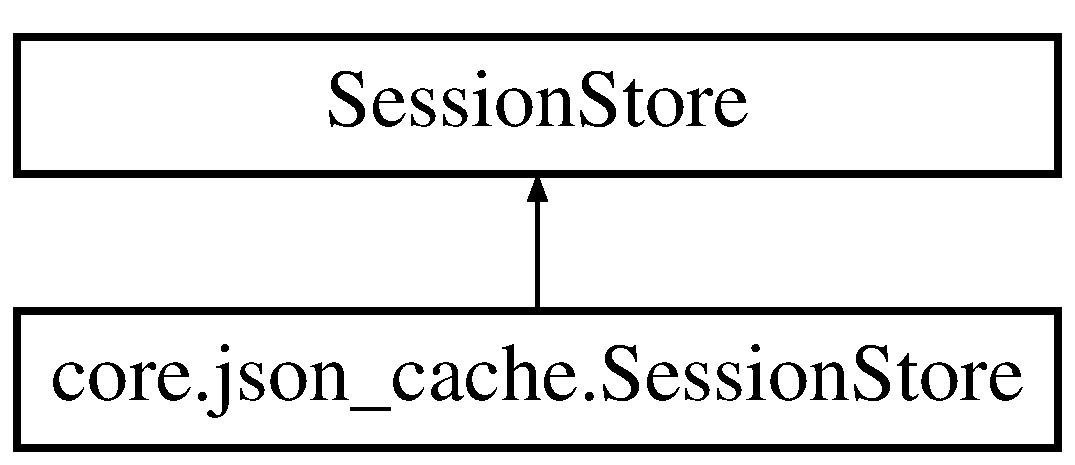
\includegraphics[height=2.000000cm]{classcore_1_1json__cache_1_1SessionStore}
\end{center}
\end{figure}
\subsection*{Public Member Functions}
\begin{DoxyCompactItemize}
\item 
def \hyperlink{classcore_1_1json__cache_1_1SessionStore_a5941414be35a2956808f376f5f40d350}{\-\_\-\-\_\-init\-\_\-\-\_\-}
\end{DoxyCompactItemize}


\subsection{Constructor \& Destructor Documentation}
\hypertarget{classcore_1_1json__cache_1_1SessionStore_a5941414be35a2956808f376f5f40d350}{\index{core\-::json\-\_\-cache\-::\-Session\-Store@{core\-::json\-\_\-cache\-::\-Session\-Store}!\-\_\-\-\_\-init\-\_\-\-\_\-@{\-\_\-\-\_\-init\-\_\-\-\_\-}}
\index{\-\_\-\-\_\-init\-\_\-\-\_\-@{\-\_\-\-\_\-init\-\_\-\-\_\-}!core::json_cache::SessionStore@{core\-::json\-\_\-cache\-::\-Session\-Store}}
\subsubsection[{\-\_\-\-\_\-init\-\_\-\-\_\-}]{\setlength{\rightskip}{0pt plus 5cm}def core.\-json\-\_\-cache.\-Session\-Store.\-\_\-\-\_\-init\-\_\-\-\_\- (
\begin{DoxyParamCaption}
\item[{}]{self, }
\item[{}]{session\-\_\-key = {\ttfamily None}}
\end{DoxyParamCaption}
)}}\label{classcore_1_1json__cache_1_1SessionStore_a5941414be35a2956808f376f5f40d350}


The documentation for this class was generated from the following file\-:\begin{DoxyCompactItemize}
\item 
/wepo/core/\hyperlink{json__cache_8py}{json\-\_\-cache.\-py}\end{DoxyCompactItemize}

\hypertarget{classcore_1_1tests_1_1SimpleTest}{\section{core.\-tests.\-Simple\-Test Class Reference}
\label{classcore_1_1tests_1_1SimpleTest}\index{core.\-tests.\-Simple\-Test@{core.\-tests.\-Simple\-Test}}
}


Simple, dummy test, to test if unit tests are working.  


Inheritance diagram for core.\-tests.\-Simple\-Test\-:\begin{figure}[H]
\begin{center}
\leavevmode
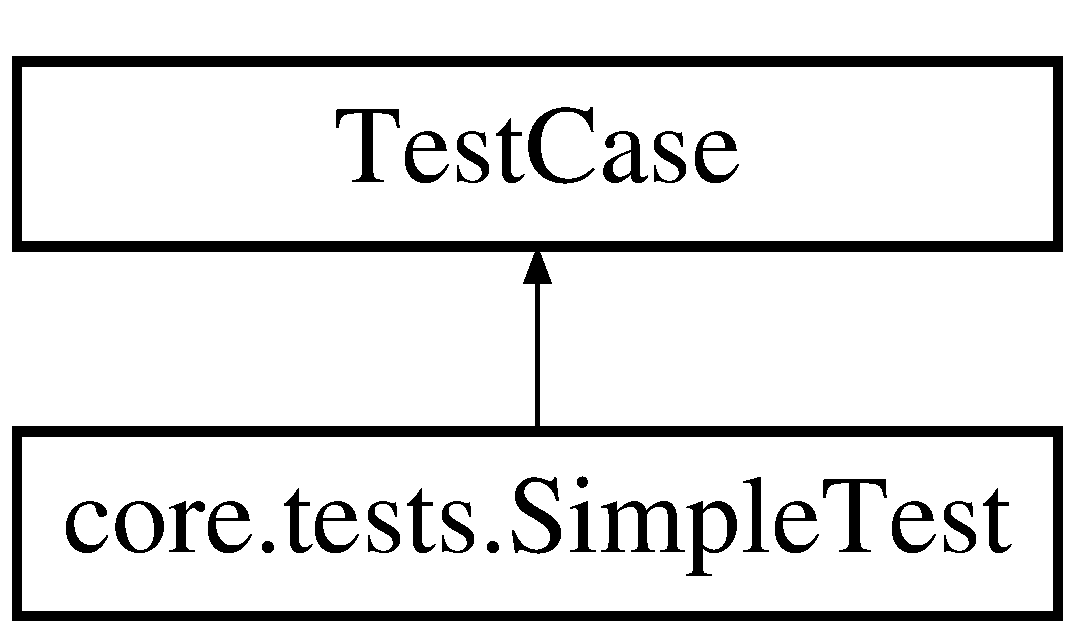
\includegraphics[height=2.000000cm]{classcore_1_1tests_1_1SimpleTest}
\end{center}
\end{figure}
\subsection*{Public Member Functions}
\begin{DoxyCompactItemize}
\item 
def \hyperlink{classcore_1_1tests_1_1SimpleTest_a06518053ac3a064da8270d1a95cd414c}{test\-\_\-basic\-\_\-addition}
\end{DoxyCompactItemize}


\subsection{Detailed Description}
Simple, dummy test, to test if unit tests are working. 

Tests that 1 + 1 always equals 2. 

\subsection{Member Function Documentation}
\hypertarget{classcore_1_1tests_1_1SimpleTest_a06518053ac3a064da8270d1a95cd414c}{\index{core\-::tests\-::\-Simple\-Test@{core\-::tests\-::\-Simple\-Test}!test\-\_\-basic\-\_\-addition@{test\-\_\-basic\-\_\-addition}}
\index{test\-\_\-basic\-\_\-addition@{test\-\_\-basic\-\_\-addition}!core::tests::SimpleTest@{core\-::tests\-::\-Simple\-Test}}
\subsubsection[{test\-\_\-basic\-\_\-addition}]{\setlength{\rightskip}{0pt plus 5cm}def core.\-tests.\-Simple\-Test.\-test\-\_\-basic\-\_\-addition (
\begin{DoxyParamCaption}
\item[{}]{self}
\end{DoxyParamCaption}
)}}\label{classcore_1_1tests_1_1SimpleTest_a06518053ac3a064da8270d1a95cd414c}


The documentation for this class was generated from the following file\-:\begin{DoxyCompactItemize}
\item 
/wepo/core/\hyperlink{tests_8py}{tests.\-py}\end{DoxyCompactItemize}

\hypertarget{classcore_1_1unit_1_1Assets_1_1TestAssets}{\section{core.\-unit.\-Assets.\-Test\-Assets Class Reference}
\label{classcore_1_1unit_1_1Assets_1_1TestAssets}\index{core.\-unit.\-Assets.\-Test\-Assets@{core.\-unit.\-Assets.\-Test\-Assets}}
}
Inheritance diagram for core.\-unit.\-Assets.\-Test\-Assets\-:\begin{figure}[H]
\begin{center}
\leavevmode
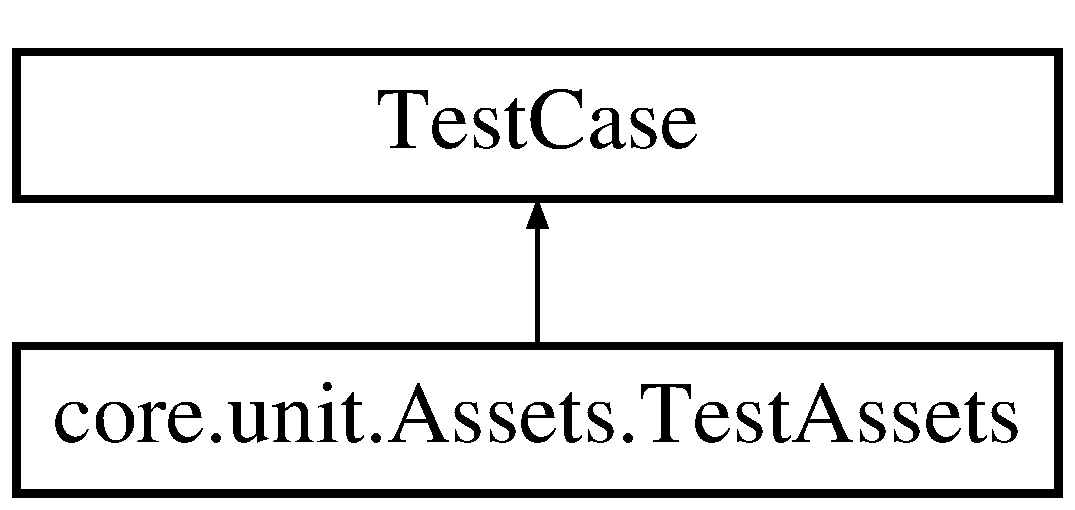
\includegraphics[height=2.000000cm]{classcore_1_1unit_1_1Assets_1_1TestAssets}
\end{center}
\end{figure}
\subsection*{Public Member Functions}
\begin{DoxyCompactItemize}
\item 
def \hyperlink{classcore_1_1unit_1_1Assets_1_1TestAssets_a2489c7550a363551f520bf8626324932}{test\-\_\-core\-\_\-user\-\_\-login\-\_\-assets}
\end{DoxyCompactItemize}


\subsection{Member Function Documentation}
\hypertarget{classcore_1_1unit_1_1Assets_1_1TestAssets_a2489c7550a363551f520bf8626324932}{\index{core\-::unit\-::\-Assets\-::\-Test\-Assets@{core\-::unit\-::\-Assets\-::\-Test\-Assets}!test\-\_\-core\-\_\-user\-\_\-login\-\_\-assets@{test\-\_\-core\-\_\-user\-\_\-login\-\_\-assets}}
\index{test\-\_\-core\-\_\-user\-\_\-login\-\_\-assets@{test\-\_\-core\-\_\-user\-\_\-login\-\_\-assets}!core::unit::Assets::TestAssets@{core\-::unit\-::\-Assets\-::\-Test\-Assets}}
\subsubsection[{test\-\_\-core\-\_\-user\-\_\-login\-\_\-assets}]{\setlength{\rightskip}{0pt plus 5cm}def core.\-unit.\-Assets.\-Test\-Assets.\-test\-\_\-core\-\_\-user\-\_\-login\-\_\-assets (
\begin{DoxyParamCaption}
\item[{}]{self}
\end{DoxyParamCaption}
)}}\label{classcore_1_1unit_1_1Assets_1_1TestAssets_a2489c7550a363551f520bf8626324932}


The documentation for this class was generated from the following file\-:\begin{DoxyCompactItemize}
\item 
/wepo/core/unit/\hyperlink{Assets_8py}{Assets.\-py}\end{DoxyCompactItemize}

\hypertarget{classcore_1_1unit_1_1Blocks_1_1TestBlocks}{\section{core.\-unit.\-Blocks.\-Test\-Blocks Class Reference}
\label{classcore_1_1unit_1_1Blocks_1_1TestBlocks}\index{core.\-unit.\-Blocks.\-Test\-Blocks@{core.\-unit.\-Blocks.\-Test\-Blocks}}
}
Inheritance diagram for core.\-unit.\-Blocks.\-Test\-Blocks\-:\begin{figure}[H]
\begin{center}
\leavevmode
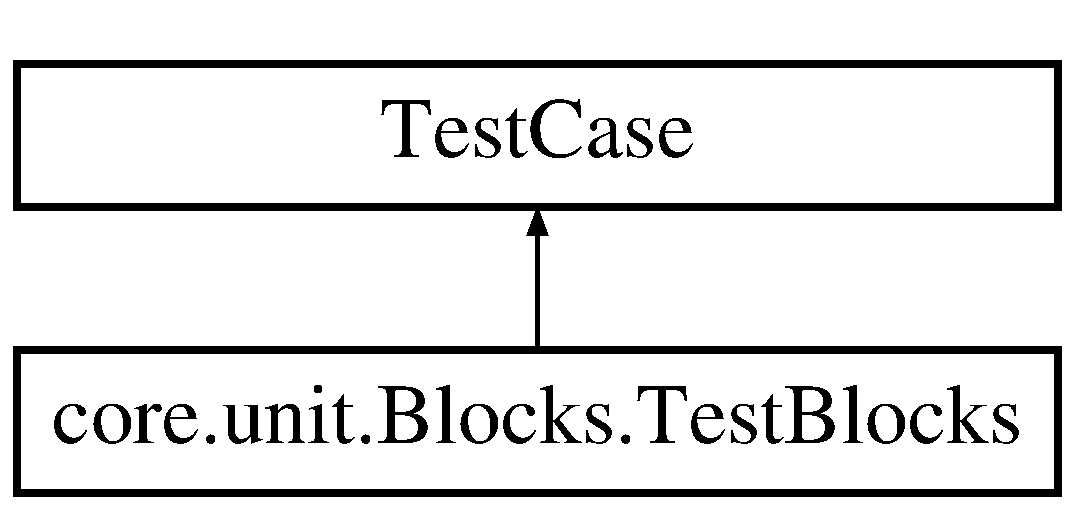
\includegraphics[height=2.000000cm]{classcore_1_1unit_1_1Blocks_1_1TestBlocks}
\end{center}
\end{figure}
\subsection*{Public Member Functions}
\begin{DoxyCompactItemize}
\item 
def \hyperlink{classcore_1_1unit_1_1Blocks_1_1TestBlocks_a9c06ebca79b765f27e8a18d4854ad3fb}{test\-\_\-admin\-\_\-blocks}
\end{DoxyCompactItemize}


\subsection{Member Function Documentation}
\hypertarget{classcore_1_1unit_1_1Blocks_1_1TestBlocks_a9c06ebca79b765f27e8a18d4854ad3fb}{\index{core\-::unit\-::\-Blocks\-::\-Test\-Blocks@{core\-::unit\-::\-Blocks\-::\-Test\-Blocks}!test\-\_\-admin\-\_\-blocks@{test\-\_\-admin\-\_\-blocks}}
\index{test\-\_\-admin\-\_\-blocks@{test\-\_\-admin\-\_\-blocks}!core::unit::Blocks::TestBlocks@{core\-::unit\-::\-Blocks\-::\-Test\-Blocks}}
\subsubsection[{test\-\_\-admin\-\_\-blocks}]{\setlength{\rightskip}{0pt plus 5cm}def core.\-unit.\-Blocks.\-Test\-Blocks.\-test\-\_\-admin\-\_\-blocks (
\begin{DoxyParamCaption}
\item[{}]{self}
\end{DoxyParamCaption}
)}}\label{classcore_1_1unit_1_1Blocks_1_1TestBlocks_a9c06ebca79b765f27e8a18d4854ad3fb}


The documentation for this class was generated from the following file\-:\begin{DoxyCompactItemize}
\item 
/wepo/core/unit/\hyperlink{Blocks_8py}{Blocks.\-py}\end{DoxyCompactItemize}

\hypertarget{classcore_1_1unit_1_1Layouts_1_1TestLayouts}{\section{core.\-unit.\-Layouts.\-Test\-Layouts Class Reference}
\label{classcore_1_1unit_1_1Layouts_1_1TestLayouts}\index{core.\-unit.\-Layouts.\-Test\-Layouts@{core.\-unit.\-Layouts.\-Test\-Layouts}}
}
Inheritance diagram for core.\-unit.\-Layouts.\-Test\-Layouts\-:\begin{figure}[H]
\begin{center}
\leavevmode
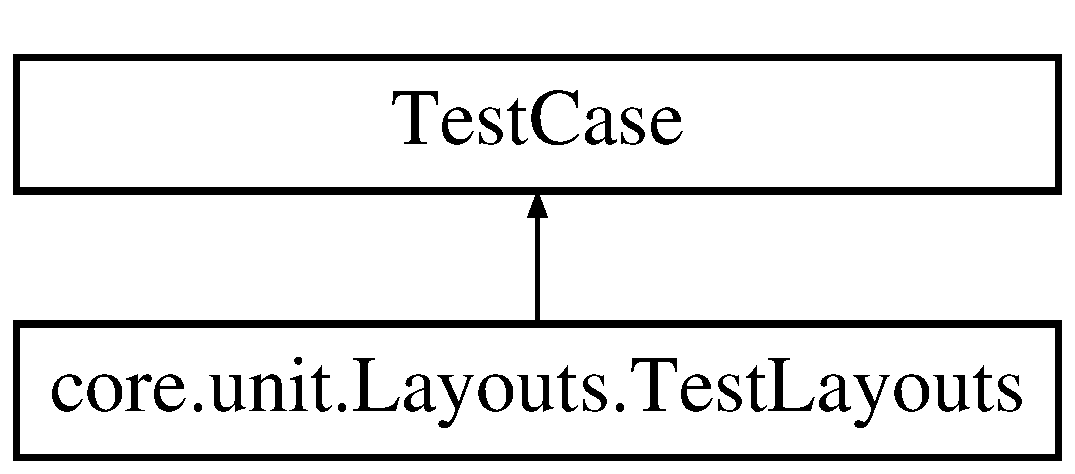
\includegraphics[height=2.000000cm]{classcore_1_1unit_1_1Layouts_1_1TestLayouts}
\end{center}
\end{figure}
\subsection*{Public Member Functions}
\begin{DoxyCompactItemize}
\item 
def \hyperlink{classcore_1_1unit_1_1Layouts_1_1TestLayouts_aded76c40b43a34a80777272b0eb1dc7a}{test\-\_\-admin\-\_\-layouts}
\end{DoxyCompactItemize}


\subsection{Member Function Documentation}
\hypertarget{classcore_1_1unit_1_1Layouts_1_1TestLayouts_aded76c40b43a34a80777272b0eb1dc7a}{\index{core\-::unit\-::\-Layouts\-::\-Test\-Layouts@{core\-::unit\-::\-Layouts\-::\-Test\-Layouts}!test\-\_\-admin\-\_\-layouts@{test\-\_\-admin\-\_\-layouts}}
\index{test\-\_\-admin\-\_\-layouts@{test\-\_\-admin\-\_\-layouts}!core::unit::Layouts::TestLayouts@{core\-::unit\-::\-Layouts\-::\-Test\-Layouts}}
\subsubsection[{test\-\_\-admin\-\_\-layouts}]{\setlength{\rightskip}{0pt plus 5cm}def core.\-unit.\-Layouts.\-Test\-Layouts.\-test\-\_\-admin\-\_\-layouts (
\begin{DoxyParamCaption}
\item[{}]{self}
\end{DoxyParamCaption}
)}}\label{classcore_1_1unit_1_1Layouts_1_1TestLayouts_aded76c40b43a34a80777272b0eb1dc7a}


The documentation for this class was generated from the following file\-:\begin{DoxyCompactItemize}
\item 
/wepo/core/unit/\hyperlink{Layouts_8py}{Layouts.\-py}\end{DoxyCompactItemize}

\hypertarget{classcore_1_1unit_1_1Permissions_1_1TestPermissions}{\section{core.\-unit.\-Permissions.\-Test\-Permissions Class Reference}
\label{classcore_1_1unit_1_1Permissions_1_1TestPermissions}\index{core.\-unit.\-Permissions.\-Test\-Permissions@{core.\-unit.\-Permissions.\-Test\-Permissions}}
}
Inheritance diagram for core.\-unit.\-Permissions.\-Test\-Permissions\-:\begin{figure}[H]
\begin{center}
\leavevmode
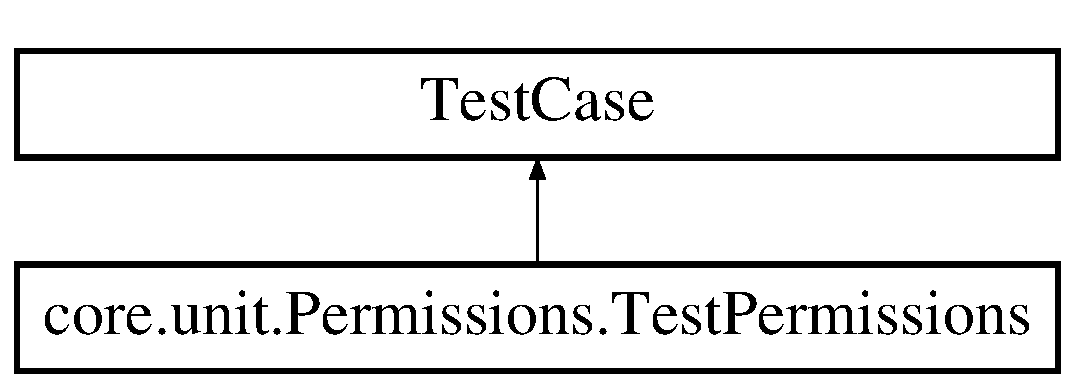
\includegraphics[height=2.000000cm]{classcore_1_1unit_1_1Permissions_1_1TestPermissions}
\end{center}
\end{figure}
\subsection*{Public Member Functions}
\begin{DoxyCompactItemize}
\item 
def \hyperlink{classcore_1_1unit_1_1Permissions_1_1TestPermissions_adfaedc4f4cae25b9839160efaae385c2}{test\-\_\-permissions}
\end{DoxyCompactItemize}


\subsection{Member Function Documentation}
\hypertarget{classcore_1_1unit_1_1Permissions_1_1TestPermissions_adfaedc4f4cae25b9839160efaae385c2}{\index{core\-::unit\-::\-Permissions\-::\-Test\-Permissions@{core\-::unit\-::\-Permissions\-::\-Test\-Permissions}!test\-\_\-permissions@{test\-\_\-permissions}}
\index{test\-\_\-permissions@{test\-\_\-permissions}!core::unit::Permissions::TestPermissions@{core\-::unit\-::\-Permissions\-::\-Test\-Permissions}}
\subsubsection[{test\-\_\-permissions}]{\setlength{\rightskip}{0pt plus 5cm}def core.\-unit.\-Permissions.\-Test\-Permissions.\-test\-\_\-permissions (
\begin{DoxyParamCaption}
\item[{}]{self}
\end{DoxyParamCaption}
)}}\label{classcore_1_1unit_1_1Permissions_1_1TestPermissions_adfaedc4f4cae25b9839160efaae385c2}


The documentation for this class was generated from the following file\-:\begin{DoxyCompactItemize}
\item 
/wepo/core/unit/\hyperlink{Permissions_8py}{Permissions.\-py}\end{DoxyCompactItemize}

\hypertarget{classcore_1_1unit_1_1Seo_1_1TestSeo}{\section{core.\-unit.\-Seo.\-Test\-Seo Class Reference}
\label{classcore_1_1unit_1_1Seo_1_1TestSeo}\index{core.\-unit.\-Seo.\-Test\-Seo@{core.\-unit.\-Seo.\-Test\-Seo}}
}
Inheritance diagram for core.\-unit.\-Seo.\-Test\-Seo\-:\begin{figure}[H]
\begin{center}
\leavevmode
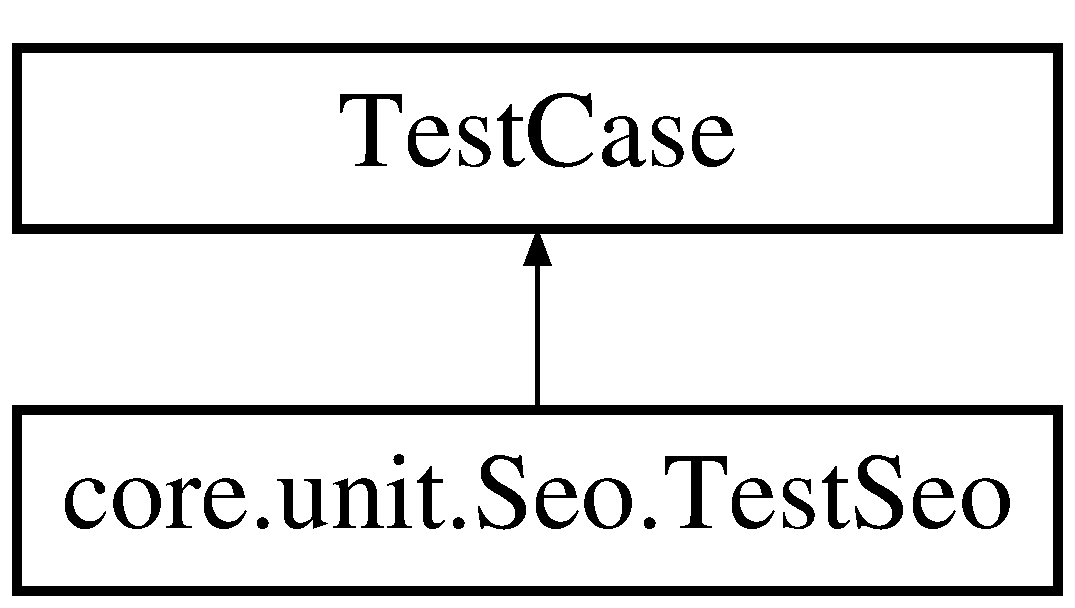
\includegraphics[height=2.000000cm]{classcore_1_1unit_1_1Seo_1_1TestSeo}
\end{center}
\end{figure}
\subsection*{Public Member Functions}
\begin{DoxyCompactItemize}
\item 
def \hyperlink{classcore_1_1unit_1_1Seo_1_1TestSeo_a38306f141b92de978c348439d314426b}{test\-\_\-error\-\_\-seo}
\end{DoxyCompactItemize}


\subsection{Member Function Documentation}
\hypertarget{classcore_1_1unit_1_1Seo_1_1TestSeo_a38306f141b92de978c348439d314426b}{\index{core\-::unit\-::\-Seo\-::\-Test\-Seo@{core\-::unit\-::\-Seo\-::\-Test\-Seo}!test\-\_\-error\-\_\-seo@{test\-\_\-error\-\_\-seo}}
\index{test\-\_\-error\-\_\-seo@{test\-\_\-error\-\_\-seo}!core::unit::Seo::TestSeo@{core\-::unit\-::\-Seo\-::\-Test\-Seo}}
\subsubsection[{test\-\_\-error\-\_\-seo}]{\setlength{\rightskip}{0pt plus 5cm}def core.\-unit.\-Seo.\-Test\-Seo.\-test\-\_\-error\-\_\-seo (
\begin{DoxyParamCaption}
\item[{}]{self}
\end{DoxyParamCaption}
)}}\label{classcore_1_1unit_1_1Seo_1_1TestSeo_a38306f141b92de978c348439d314426b}


The documentation for this class was generated from the following file\-:\begin{DoxyCompactItemize}
\item 
/wepo/core/unit/\hyperlink{Seo_8py}{Seo.\-py}\end{DoxyCompactItemize}

\hypertarget{classcore_1_1unit_1_1WepoGeneric_1_1TestWepoGeneric}{\section{core.\-unit.\-Wepo\-Generic.\-Test\-Wepo\-Generic Class Reference}
\label{classcore_1_1unit_1_1WepoGeneric_1_1TestWepoGeneric}\index{core.\-unit.\-Wepo\-Generic.\-Test\-Wepo\-Generic@{core.\-unit.\-Wepo\-Generic.\-Test\-Wepo\-Generic}}
}
Inheritance diagram for core.\-unit.\-Wepo\-Generic.\-Test\-Wepo\-Generic\-:\begin{figure}[H]
\begin{center}
\leavevmode
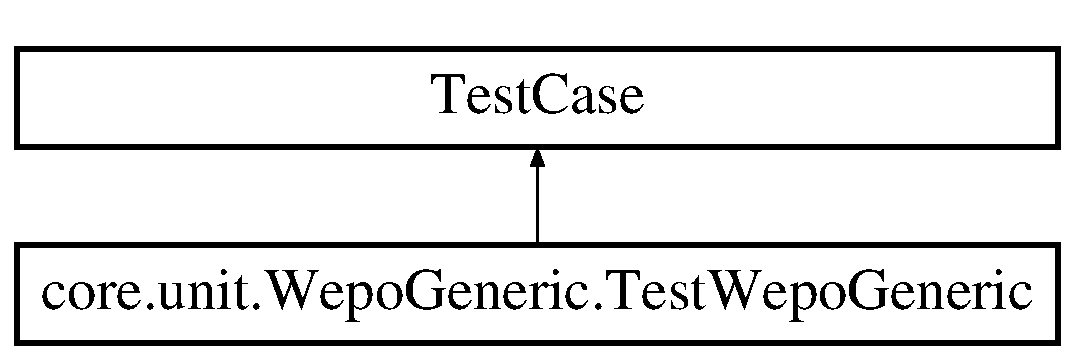
\includegraphics[height=2.000000cm]{classcore_1_1unit_1_1WepoGeneric_1_1TestWepoGeneric}
\end{center}
\end{figure}
\subsection*{Public Member Functions}
\begin{DoxyCompactItemize}
\item 
def \hyperlink{classcore_1_1unit_1_1WepoGeneric_1_1TestWepoGeneric_a4017a0ce9649f413c51cca1a5cb6e33b}{test\-\_\-should\-\_\-init\-\_\-with\-\_\-one\-\_\-dict}
\item 
def \hyperlink{classcore_1_1unit_1_1WepoGeneric_1_1TestWepoGeneric_acd805191665e02c2ed7aba7f443c8214}{test\-\_\-should\-\_\-not\-\_\-change\-\_\-values\-\_\-by\-\_\-inited\-\_\-dict}
\item 
def \hyperlink{classcore_1_1unit_1_1WepoGeneric_1_1TestWepoGeneric_a0a8afb004d38748b28d37a959d35e7c6}{test\-\_\-get\-\_\-item}
\item 
def \hyperlink{classcore_1_1unit_1_1WepoGeneric_1_1TestWepoGeneric_affd16d2807d3ae00f680c10614f9c4c2}{test\-\_\-set\-\_\-item}
\item 
def \hyperlink{classcore_1_1unit_1_1WepoGeneric_1_1TestWepoGeneric_a6dbbc9d768579bb131dca8ada087b58b}{test\-\_\-del\-\_\-attr}
\item 
def \hyperlink{classcore_1_1unit_1_1WepoGeneric_1_1TestWepoGeneric_a82e9f73676915a5507e5f57304ce268e}{test\-\_\-in\-\_\-should\-\_\-work\-\_\-like\-\_\-in\-\_\-dict}
\item 
def \hyperlink{classcore_1_1unit_1_1WepoGeneric_1_1TestWepoGeneric_aa352248252742e4058712dd7940998e9}{test\-\_\-len\-\_\-should\-\_\-work\-\_\-like\-\_\-in\-\_\-dict}
\item 
def \hyperlink{classcore_1_1unit_1_1WepoGeneric_1_1TestWepoGeneric_ac7bcb2eea99b5ed3099dba266eb8f1f4}{test\-\_\-repr}
\item 
def \hyperlink{classcore_1_1unit_1_1WepoGeneric_1_1TestWepoGeneric_aca99d5e5c1102d29331eda4a4888b759}{test\-\_\-equal}
\end{DoxyCompactItemize}


\subsection{Member Function Documentation}
\hypertarget{classcore_1_1unit_1_1WepoGeneric_1_1TestWepoGeneric_a6dbbc9d768579bb131dca8ada087b58b}{\index{core\-::unit\-::\-Wepo\-Generic\-::\-Test\-Wepo\-Generic@{core\-::unit\-::\-Wepo\-Generic\-::\-Test\-Wepo\-Generic}!test\-\_\-del\-\_\-attr@{test\-\_\-del\-\_\-attr}}
\index{test\-\_\-del\-\_\-attr@{test\-\_\-del\-\_\-attr}!core::unit::WepoGeneric::TestWepoGeneric@{core\-::unit\-::\-Wepo\-Generic\-::\-Test\-Wepo\-Generic}}
\subsubsection[{test\-\_\-del\-\_\-attr}]{\setlength{\rightskip}{0pt plus 5cm}def core.\-unit.\-Wepo\-Generic.\-Test\-Wepo\-Generic.\-test\-\_\-del\-\_\-attr (
\begin{DoxyParamCaption}
\item[{}]{self}
\end{DoxyParamCaption}
)}}\label{classcore_1_1unit_1_1WepoGeneric_1_1TestWepoGeneric_a6dbbc9d768579bb131dca8ada087b58b}
\hypertarget{classcore_1_1unit_1_1WepoGeneric_1_1TestWepoGeneric_aca99d5e5c1102d29331eda4a4888b759}{\index{core\-::unit\-::\-Wepo\-Generic\-::\-Test\-Wepo\-Generic@{core\-::unit\-::\-Wepo\-Generic\-::\-Test\-Wepo\-Generic}!test\-\_\-equal@{test\-\_\-equal}}
\index{test\-\_\-equal@{test\-\_\-equal}!core::unit::WepoGeneric::TestWepoGeneric@{core\-::unit\-::\-Wepo\-Generic\-::\-Test\-Wepo\-Generic}}
\subsubsection[{test\-\_\-equal}]{\setlength{\rightskip}{0pt plus 5cm}def core.\-unit.\-Wepo\-Generic.\-Test\-Wepo\-Generic.\-test\-\_\-equal (
\begin{DoxyParamCaption}
\item[{}]{self}
\end{DoxyParamCaption}
)}}\label{classcore_1_1unit_1_1WepoGeneric_1_1TestWepoGeneric_aca99d5e5c1102d29331eda4a4888b759}
\hypertarget{classcore_1_1unit_1_1WepoGeneric_1_1TestWepoGeneric_a0a8afb004d38748b28d37a959d35e7c6}{\index{core\-::unit\-::\-Wepo\-Generic\-::\-Test\-Wepo\-Generic@{core\-::unit\-::\-Wepo\-Generic\-::\-Test\-Wepo\-Generic}!test\-\_\-get\-\_\-item@{test\-\_\-get\-\_\-item}}
\index{test\-\_\-get\-\_\-item@{test\-\_\-get\-\_\-item}!core::unit::WepoGeneric::TestWepoGeneric@{core\-::unit\-::\-Wepo\-Generic\-::\-Test\-Wepo\-Generic}}
\subsubsection[{test\-\_\-get\-\_\-item}]{\setlength{\rightskip}{0pt plus 5cm}def core.\-unit.\-Wepo\-Generic.\-Test\-Wepo\-Generic.\-test\-\_\-get\-\_\-item (
\begin{DoxyParamCaption}
\item[{}]{self}
\end{DoxyParamCaption}
)}}\label{classcore_1_1unit_1_1WepoGeneric_1_1TestWepoGeneric_a0a8afb004d38748b28d37a959d35e7c6}
\hypertarget{classcore_1_1unit_1_1WepoGeneric_1_1TestWepoGeneric_a82e9f73676915a5507e5f57304ce268e}{\index{core\-::unit\-::\-Wepo\-Generic\-::\-Test\-Wepo\-Generic@{core\-::unit\-::\-Wepo\-Generic\-::\-Test\-Wepo\-Generic}!test\-\_\-in\-\_\-should\-\_\-work\-\_\-like\-\_\-in\-\_\-dict@{test\-\_\-in\-\_\-should\-\_\-work\-\_\-like\-\_\-in\-\_\-dict}}
\index{test\-\_\-in\-\_\-should\-\_\-work\-\_\-like\-\_\-in\-\_\-dict@{test\-\_\-in\-\_\-should\-\_\-work\-\_\-like\-\_\-in\-\_\-dict}!core::unit::WepoGeneric::TestWepoGeneric@{core\-::unit\-::\-Wepo\-Generic\-::\-Test\-Wepo\-Generic}}
\subsubsection[{test\-\_\-in\-\_\-should\-\_\-work\-\_\-like\-\_\-in\-\_\-dict}]{\setlength{\rightskip}{0pt plus 5cm}def core.\-unit.\-Wepo\-Generic.\-Test\-Wepo\-Generic.\-test\-\_\-in\-\_\-should\-\_\-work\-\_\-like\-\_\-in\-\_\-dict (
\begin{DoxyParamCaption}
\item[{}]{self}
\end{DoxyParamCaption}
)}}\label{classcore_1_1unit_1_1WepoGeneric_1_1TestWepoGeneric_a82e9f73676915a5507e5f57304ce268e}
\hypertarget{classcore_1_1unit_1_1WepoGeneric_1_1TestWepoGeneric_aa352248252742e4058712dd7940998e9}{\index{core\-::unit\-::\-Wepo\-Generic\-::\-Test\-Wepo\-Generic@{core\-::unit\-::\-Wepo\-Generic\-::\-Test\-Wepo\-Generic}!test\-\_\-len\-\_\-should\-\_\-work\-\_\-like\-\_\-in\-\_\-dict@{test\-\_\-len\-\_\-should\-\_\-work\-\_\-like\-\_\-in\-\_\-dict}}
\index{test\-\_\-len\-\_\-should\-\_\-work\-\_\-like\-\_\-in\-\_\-dict@{test\-\_\-len\-\_\-should\-\_\-work\-\_\-like\-\_\-in\-\_\-dict}!core::unit::WepoGeneric::TestWepoGeneric@{core\-::unit\-::\-Wepo\-Generic\-::\-Test\-Wepo\-Generic}}
\subsubsection[{test\-\_\-len\-\_\-should\-\_\-work\-\_\-like\-\_\-in\-\_\-dict}]{\setlength{\rightskip}{0pt plus 5cm}def core.\-unit.\-Wepo\-Generic.\-Test\-Wepo\-Generic.\-test\-\_\-len\-\_\-should\-\_\-work\-\_\-like\-\_\-in\-\_\-dict (
\begin{DoxyParamCaption}
\item[{}]{self}
\end{DoxyParamCaption}
)}}\label{classcore_1_1unit_1_1WepoGeneric_1_1TestWepoGeneric_aa352248252742e4058712dd7940998e9}
\hypertarget{classcore_1_1unit_1_1WepoGeneric_1_1TestWepoGeneric_ac7bcb2eea99b5ed3099dba266eb8f1f4}{\index{core\-::unit\-::\-Wepo\-Generic\-::\-Test\-Wepo\-Generic@{core\-::unit\-::\-Wepo\-Generic\-::\-Test\-Wepo\-Generic}!test\-\_\-repr@{test\-\_\-repr}}
\index{test\-\_\-repr@{test\-\_\-repr}!core::unit::WepoGeneric::TestWepoGeneric@{core\-::unit\-::\-Wepo\-Generic\-::\-Test\-Wepo\-Generic}}
\subsubsection[{test\-\_\-repr}]{\setlength{\rightskip}{0pt plus 5cm}def core.\-unit.\-Wepo\-Generic.\-Test\-Wepo\-Generic.\-test\-\_\-repr (
\begin{DoxyParamCaption}
\item[{}]{self}
\end{DoxyParamCaption}
)}}\label{classcore_1_1unit_1_1WepoGeneric_1_1TestWepoGeneric_ac7bcb2eea99b5ed3099dba266eb8f1f4}
\hypertarget{classcore_1_1unit_1_1WepoGeneric_1_1TestWepoGeneric_affd16d2807d3ae00f680c10614f9c4c2}{\index{core\-::unit\-::\-Wepo\-Generic\-::\-Test\-Wepo\-Generic@{core\-::unit\-::\-Wepo\-Generic\-::\-Test\-Wepo\-Generic}!test\-\_\-set\-\_\-item@{test\-\_\-set\-\_\-item}}
\index{test\-\_\-set\-\_\-item@{test\-\_\-set\-\_\-item}!core::unit::WepoGeneric::TestWepoGeneric@{core\-::unit\-::\-Wepo\-Generic\-::\-Test\-Wepo\-Generic}}
\subsubsection[{test\-\_\-set\-\_\-item}]{\setlength{\rightskip}{0pt plus 5cm}def core.\-unit.\-Wepo\-Generic.\-Test\-Wepo\-Generic.\-test\-\_\-set\-\_\-item (
\begin{DoxyParamCaption}
\item[{}]{self}
\end{DoxyParamCaption}
)}}\label{classcore_1_1unit_1_1WepoGeneric_1_1TestWepoGeneric_affd16d2807d3ae00f680c10614f9c4c2}
\hypertarget{classcore_1_1unit_1_1WepoGeneric_1_1TestWepoGeneric_a4017a0ce9649f413c51cca1a5cb6e33b}{\index{core\-::unit\-::\-Wepo\-Generic\-::\-Test\-Wepo\-Generic@{core\-::unit\-::\-Wepo\-Generic\-::\-Test\-Wepo\-Generic}!test\-\_\-should\-\_\-init\-\_\-with\-\_\-one\-\_\-dict@{test\-\_\-should\-\_\-init\-\_\-with\-\_\-one\-\_\-dict}}
\index{test\-\_\-should\-\_\-init\-\_\-with\-\_\-one\-\_\-dict@{test\-\_\-should\-\_\-init\-\_\-with\-\_\-one\-\_\-dict}!core::unit::WepoGeneric::TestWepoGeneric@{core\-::unit\-::\-Wepo\-Generic\-::\-Test\-Wepo\-Generic}}
\subsubsection[{test\-\_\-should\-\_\-init\-\_\-with\-\_\-one\-\_\-dict}]{\setlength{\rightskip}{0pt plus 5cm}def core.\-unit.\-Wepo\-Generic.\-Test\-Wepo\-Generic.\-test\-\_\-should\-\_\-init\-\_\-with\-\_\-one\-\_\-dict (
\begin{DoxyParamCaption}
\item[{}]{self}
\end{DoxyParamCaption}
)}}\label{classcore_1_1unit_1_1WepoGeneric_1_1TestWepoGeneric_a4017a0ce9649f413c51cca1a5cb6e33b}
\hypertarget{classcore_1_1unit_1_1WepoGeneric_1_1TestWepoGeneric_acd805191665e02c2ed7aba7f443c8214}{\index{core\-::unit\-::\-Wepo\-Generic\-::\-Test\-Wepo\-Generic@{core\-::unit\-::\-Wepo\-Generic\-::\-Test\-Wepo\-Generic}!test\-\_\-should\-\_\-not\-\_\-change\-\_\-values\-\_\-by\-\_\-inited\-\_\-dict@{test\-\_\-should\-\_\-not\-\_\-change\-\_\-values\-\_\-by\-\_\-inited\-\_\-dict}}
\index{test\-\_\-should\-\_\-not\-\_\-change\-\_\-values\-\_\-by\-\_\-inited\-\_\-dict@{test\-\_\-should\-\_\-not\-\_\-change\-\_\-values\-\_\-by\-\_\-inited\-\_\-dict}!core::unit::WepoGeneric::TestWepoGeneric@{core\-::unit\-::\-Wepo\-Generic\-::\-Test\-Wepo\-Generic}}
\subsubsection[{test\-\_\-should\-\_\-not\-\_\-change\-\_\-values\-\_\-by\-\_\-inited\-\_\-dict}]{\setlength{\rightskip}{0pt plus 5cm}def core.\-unit.\-Wepo\-Generic.\-Test\-Wepo\-Generic.\-test\-\_\-should\-\_\-not\-\_\-change\-\_\-values\-\_\-by\-\_\-inited\-\_\-dict (
\begin{DoxyParamCaption}
\item[{}]{self}
\end{DoxyParamCaption}
)}}\label{classcore_1_1unit_1_1WepoGeneric_1_1TestWepoGeneric_acd805191665e02c2ed7aba7f443c8214}


The documentation for this class was generated from the following file\-:\begin{DoxyCompactItemize}
\item 
/wepo/core/unit/\hyperlink{WepoGeneric_8py}{Wepo\-Generic.\-py}\end{DoxyCompactItemize}

\hypertarget{classcore_1_1json__cache_1_1Unpickler}{\section{core.\-json\-\_\-cache.\-Unpickler Class Reference}
\label{classcore_1_1json__cache_1_1Unpickler}\index{core.\-json\-\_\-cache.\-Unpickler@{core.\-json\-\_\-cache.\-Unpickler}}
}
Inheritance diagram for core.\-json\-\_\-cache.\-Unpickler\-:\begin{figure}[H]
\begin{center}
\leavevmode
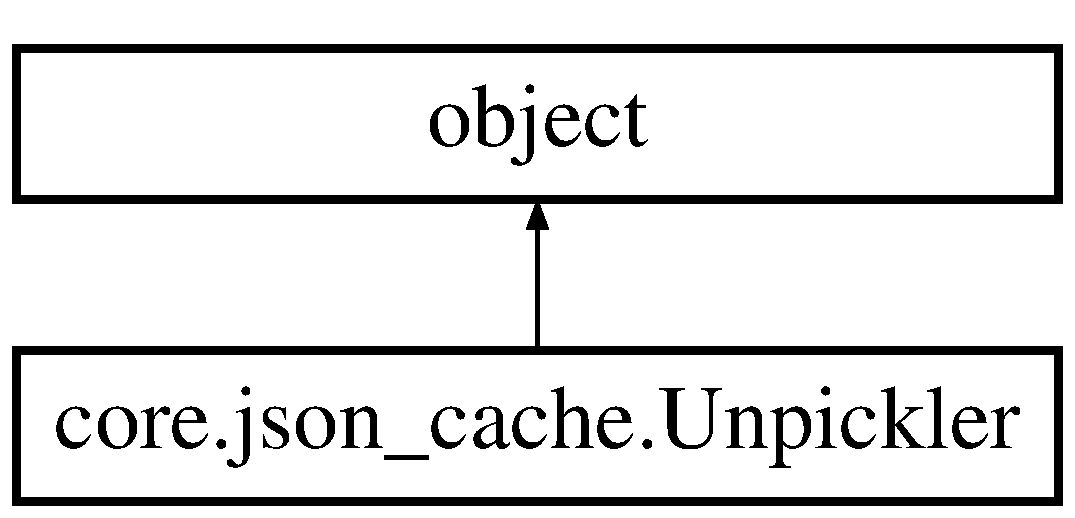
\includegraphics[height=2.000000cm]{classcore_1_1json__cache_1_1Unpickler}
\end{center}
\end{figure}
\subsection*{Public Member Functions}
\begin{DoxyCompactItemize}
\item 
def \hyperlink{classcore_1_1json__cache_1_1Unpickler_ab3d269ed6f3e66b38dc19587bb0320d5}{\-\_\-\-\_\-init\-\_\-\-\_\-}
\item 
def \hyperlink{classcore_1_1json__cache_1_1Unpickler_a150b6d3fc461ba17e350a91a505fecf8}{load}
\end{DoxyCompactItemize}
\subsection*{Public Attributes}
\begin{DoxyCompactItemize}
\item 
\hyperlink{classcore_1_1json__cache_1_1Unpickler_a0374e0ee3be62da5c217978dbb41d276}{fp}
\end{DoxyCompactItemize}


\subsection{Constructor \& Destructor Documentation}
\hypertarget{classcore_1_1json__cache_1_1Unpickler_ab3d269ed6f3e66b38dc19587bb0320d5}{\index{core\-::json\-\_\-cache\-::\-Unpickler@{core\-::json\-\_\-cache\-::\-Unpickler}!\-\_\-\-\_\-init\-\_\-\-\_\-@{\-\_\-\-\_\-init\-\_\-\-\_\-}}
\index{\-\_\-\-\_\-init\-\_\-\-\_\-@{\-\_\-\-\_\-init\-\_\-\-\_\-}!core::json_cache::Unpickler@{core\-::json\-\_\-cache\-::\-Unpickler}}
\subsubsection[{\-\_\-\-\_\-init\-\_\-\-\_\-}]{\setlength{\rightskip}{0pt plus 5cm}def core.\-json\-\_\-cache.\-Unpickler.\-\_\-\-\_\-init\-\_\-\-\_\- (
\begin{DoxyParamCaption}
\item[{}]{self, }
\item[{}]{fp, }
\item[{}]{args, }
\item[{}]{argv}
\end{DoxyParamCaption}
)}}\label{classcore_1_1json__cache_1_1Unpickler_ab3d269ed6f3e66b38dc19587bb0320d5}


\subsection{Member Function Documentation}
\hypertarget{classcore_1_1json__cache_1_1Unpickler_a150b6d3fc461ba17e350a91a505fecf8}{\index{core\-::json\-\_\-cache\-::\-Unpickler@{core\-::json\-\_\-cache\-::\-Unpickler}!load@{load}}
\index{load@{load}!core::json_cache::Unpickler@{core\-::json\-\_\-cache\-::\-Unpickler}}
\subsubsection[{load}]{\setlength{\rightskip}{0pt plus 5cm}def core.\-json\-\_\-cache.\-Unpickler.\-load (
\begin{DoxyParamCaption}
\item[{}]{self}
\end{DoxyParamCaption}
)}}\label{classcore_1_1json__cache_1_1Unpickler_a150b6d3fc461ba17e350a91a505fecf8}


\subsection{Member Data Documentation}
\hypertarget{classcore_1_1json__cache_1_1Unpickler_a0374e0ee3be62da5c217978dbb41d276}{\index{core\-::json\-\_\-cache\-::\-Unpickler@{core\-::json\-\_\-cache\-::\-Unpickler}!fp@{fp}}
\index{fp@{fp}!core::json_cache::Unpickler@{core\-::json\-\_\-cache\-::\-Unpickler}}
\subsubsection[{fp}]{\setlength{\rightskip}{0pt plus 5cm}core.\-json\-\_\-cache.\-Unpickler.\-fp}}\label{classcore_1_1json__cache_1_1Unpickler_a0374e0ee3be62da5c217978dbb41d276}


The documentation for this class was generated from the following file\-:\begin{DoxyCompactItemize}
\item 
/wepo/core/\hyperlink{json__cache_8py}{json\-\_\-cache.\-py}\end{DoxyCompactItemize}

\hypertarget{classcore_1_1models_1_1User}{\section{core.\-models.\-User Class Reference}
\label{classcore_1_1models_1_1User}\index{core.\-models.\-User@{core.\-models.\-User}}
}


\hyperlink{classcore_1_1models_1_1User}{User}.  


Inheritance diagram for core.\-models.\-User\-:\begin{figure}[H]
\begin{center}
\leavevmode
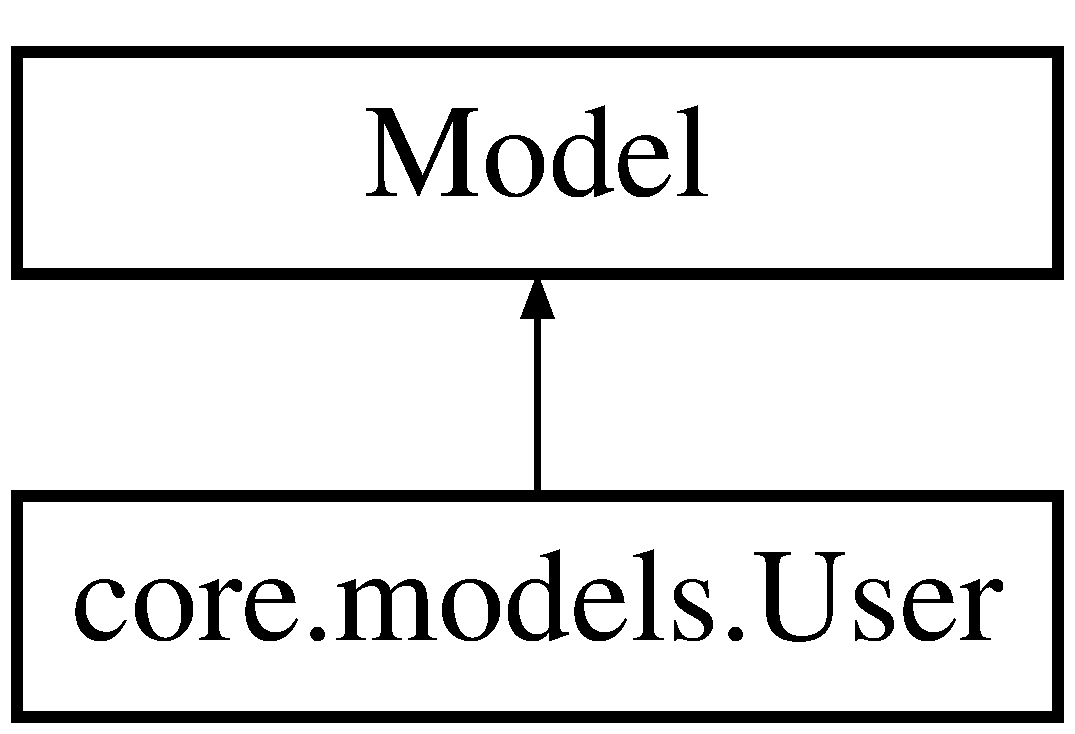
\includegraphics[height=2.000000cm]{classcore_1_1models_1_1User}
\end{center}
\end{figure}
\subsection*{Classes}
\begin{DoxyCompactItemize}
\item 
class \hyperlink{classcore_1_1models_1_1User_1_1Meta}{Meta}
\end{DoxyCompactItemize}
\subsection*{Public Member Functions}
\begin{DoxyCompactItemize}
\item 
def \hyperlink{classcore_1_1models_1_1User_a5c083b460e2d14df907edde626f3df4d}{\-\_\-\-\_\-unicode\-\_\-\-\_\-}
\item 
def \hyperlink{classcore_1_1models_1_1User_aafe570b9f5a7f23c072d5fdb1e17ad13}{save}
\begin{DoxyCompactList}\small\item\em Custom save method. \end{DoxyCompactList}\item 
def \hyperlink{classcore_1_1models_1_1User_a72865af96fbe29266f8a6131643170b0}{get\-\_\-seo}
\begin{DoxyCompactList}\small\item\em Get seo link. \end{DoxyCompactList}\end{DoxyCompactItemize}
\subsection*{Public Attributes}
\begin{DoxyCompactItemize}
\item 
\hyperlink{classcore_1_1models_1_1User_a850844de5beed6acc7ce8548e56b40f6}{key\-\_\-name}
\item 
\hyperlink{classcore_1_1models_1_1User_a7d320bc1c53745b1f8ca4f91e3cc19ea}{password}
\end{DoxyCompactItemize}
\subsection*{Static Public Attributes}
\begin{DoxyCompactItemize}
\item 
tuple \hyperlink{classcore_1_1models_1_1User_a214f7506978bd5f697a493f1b4f83553}{email} = dmodels.\-Email\-Field(db\-\_\-index=True)
\begin{DoxyCompactList}\small\item\em \hyperlink{classcore_1_1models_1_1User}{User} email address for authentication. \end{DoxyCompactList}\item 
tuple \hyperlink{classcore_1_1models_1_1User_a7d320bc1c53745b1f8ca4f91e3cc19ea}{password} = dmodels.\-Char\-Field(max\-\_\-length=64, db\-\_\-index=True)
\begin{DoxyCompactList}\small\item\em \hyperlink{classcore_1_1models_1_1User}{User} password for authentication. \end{DoxyCompactList}\item 
tuple \hyperlink{classcore_1_1models_1_1User_a6e3378459abae4fc27fcd46d1cd24990}{name} = dmodels.\-Char\-Field(max\-\_\-length=128, db\-\_\-index=True)
\begin{DoxyCompactList}\small\item\em \hyperlink{classcore_1_1models_1_1User}{User} name. \end{DoxyCompactList}\item 
tuple \hyperlink{classcore_1_1models_1_1User_a3804f136ea7cba3a9611f8432450ed4c}{surname} = dmodels.\-Char\-Field(max\-\_\-length=128, db\-\_\-index=True)
\begin{DoxyCompactList}\small\item\em \hyperlink{classcore_1_1models_1_1User}{User} surname. \end{DoxyCompactList}\item 
tuple \hyperlink{classcore_1_1models_1_1User_a17a29647bdff999f6f8ffc3bf744dd10}{groups} = dmodels.\-Many\-To\-Many\-Field(\hyperlink{classcore_1_1models_1_1Group}{Group})
\begin{DoxyCompactList}\small\item\em List of groups in user. \end{DoxyCompactList}\item 
tuple \hyperlink{classcore_1_1models_1_1User_a784eb0d695f930aeb18eeb4f7f8a166e}{permissions} = \hyperlink{classcore_1_1fields_1_1JsonField}{Json\-Field}(null=True, blank=True)
\begin{DoxyCompactList}\small\item\em List of permissions for user. \end{DoxyCompactList}\item 
tuple \hyperlink{classcore_1_1models_1_1User_ac92e0f9b0871d62b4cb283be3eb44f64}{addresses} = dmodels.\-Many\-To\-Many\-Field(\hyperlink{classcore_1_1models_1_1Address}{Address})
\begin{DoxyCompactList}\small\item\em List of addresses for user. \end{DoxyCompactList}\item 
tuple \hyperlink{classcore_1_1models_1_1User_a95cfe2aedf4dea7b41e0983035663e43}{last\-\_\-login} = dmodels.\-Date\-Time\-Field(null=True, blank=True, db\-\_\-index=True)
\begin{DoxyCompactList}\small\item\em Date time of last login. \end{DoxyCompactList}\item 
tuple \hyperlink{classcore_1_1models_1_1User_ad67e2fdbefe9f02c44070d697cf9faa1}{image} = dmodels.\-Foreign\-Key(\hyperlink{classcore_1_1models_1_1File}{File}, null=True, blank=True)
\item 
tuple \hyperlink{classcore_1_1models_1_1User_a230fb79dd5dd210ea52c4c35cbe122e2}{date\-\_\-of\-\_\-birth} = dmodels.\-Date\-Time\-Field(db\-\_\-index=True, null=True, blank=True)
\begin{DoxyCompactList}\small\item\em Date of birth. \end{DoxyCompactList}\item 
tuple \hyperlink{classcore_1_1models_1_1User_a7dc05b5317795603bcd3ca4dbb5cca8f}{gender} = dmodels.\-Char\-Field(max\-\_\-length=6, db\-\_\-index=True)
\begin{DoxyCompactList}\small\item\em \hyperlink{classcore_1_1models_1_1User}{User} gender. \end{DoxyCompactList}\end{DoxyCompactItemize}


\subsection{Detailed Description}
\hyperlink{classcore_1_1models_1_1User}{User}. 

Core user to login into the system etc. 

\subsection{Member Function Documentation}
\hypertarget{classcore_1_1models_1_1User_a5c083b460e2d14df907edde626f3df4d}{\index{core\-::models\-::\-User@{core\-::models\-::\-User}!\-\_\-\-\_\-unicode\-\_\-\-\_\-@{\-\_\-\-\_\-unicode\-\_\-\-\_\-}}
\index{\-\_\-\-\_\-unicode\-\_\-\-\_\-@{\-\_\-\-\_\-unicode\-\_\-\-\_\-}!core::models::User@{core\-::models\-::\-User}}
\subsubsection[{\-\_\-\-\_\-unicode\-\_\-\-\_\-}]{\setlength{\rightskip}{0pt plus 5cm}def core.\-models.\-User.\-\_\-\-\_\-unicode\-\_\-\-\_\- (
\begin{DoxyParamCaption}
\item[{}]{self}
\end{DoxyParamCaption}
)}}\label{classcore_1_1models_1_1User_a5c083b460e2d14df907edde626f3df4d}
\hypertarget{classcore_1_1models_1_1User_a72865af96fbe29266f8a6131643170b0}{\index{core\-::models\-::\-User@{core\-::models\-::\-User}!get\-\_\-seo@{get\-\_\-seo}}
\index{get\-\_\-seo@{get\-\_\-seo}!core::models::User@{core\-::models\-::\-User}}
\subsubsection[{get\-\_\-seo}]{\setlength{\rightskip}{0pt plus 5cm}def core.\-models.\-User.\-get\-\_\-seo (
\begin{DoxyParamCaption}
\item[{}]{self}
\end{DoxyParamCaption}
)}}\label{classcore_1_1models_1_1User_a72865af96fbe29266f8a6131643170b0}


Get seo link. 

\hypertarget{classcore_1_1models_1_1User_aafe570b9f5a7f23c072d5fdb1e17ad13}{\index{core\-::models\-::\-User@{core\-::models\-::\-User}!save@{save}}
\index{save@{save}!core::models::User@{core\-::models\-::\-User}}
\subsubsection[{save}]{\setlength{\rightskip}{0pt plus 5cm}def core.\-models.\-User.\-save (
\begin{DoxyParamCaption}
\item[{}]{self, }
\item[{}]{force\-\_\-insert = {\ttfamily False}, }
\item[{}]{force\-\_\-update = {\ttfamily False}, }
\item[{}]{using = {\ttfamily None}, }
\item[{}]{update\-\_\-fields = {\ttfamily None}, }
\item[{}]{change\-\_\-password = {\ttfamily True}}
\end{DoxyParamCaption}
)}}\label{classcore_1_1models_1_1User_aafe570b9f5a7f23c072d5fdb1e17ad13}


Custom save method. 



\subsection{Member Data Documentation}
\hypertarget{classcore_1_1models_1_1User_ac92e0f9b0871d62b4cb283be3eb44f64}{\index{core\-::models\-::\-User@{core\-::models\-::\-User}!addresses@{addresses}}
\index{addresses@{addresses}!core::models::User@{core\-::models\-::\-User}}
\subsubsection[{addresses}]{\setlength{\rightskip}{0pt plus 5cm}core.\-models.\-User.\-addresses = dmodels.\-Many\-To\-Many\-Field({\bf Address})\hspace{0.3cm}{\ttfamily [static]}}}\label{classcore_1_1models_1_1User_ac92e0f9b0871d62b4cb283be3eb44f64}


List of addresses for user. 

\hypertarget{classcore_1_1models_1_1User_a230fb79dd5dd210ea52c4c35cbe122e2}{\index{core\-::models\-::\-User@{core\-::models\-::\-User}!date\-\_\-of\-\_\-birth@{date\-\_\-of\-\_\-birth}}
\index{date\-\_\-of\-\_\-birth@{date\-\_\-of\-\_\-birth}!core::models::User@{core\-::models\-::\-User}}
\subsubsection[{date\-\_\-of\-\_\-birth}]{\setlength{\rightskip}{0pt plus 5cm}core.\-models.\-User.\-date\-\_\-of\-\_\-birth = dmodels.\-Date\-Time\-Field(db\-\_\-index=True, null=True, blank=True)\hspace{0.3cm}{\ttfamily [static]}}}\label{classcore_1_1models_1_1User_a230fb79dd5dd210ea52c4c35cbe122e2}


Date of birth. 

\hypertarget{classcore_1_1models_1_1User_a214f7506978bd5f697a493f1b4f83553}{\index{core\-::models\-::\-User@{core\-::models\-::\-User}!email@{email}}
\index{email@{email}!core::models::User@{core\-::models\-::\-User}}
\subsubsection[{email}]{\setlength{\rightskip}{0pt plus 5cm}core.\-models.\-User.\-email = dmodels.\-Email\-Field(db\-\_\-index=True)\hspace{0.3cm}{\ttfamily [static]}}}\label{classcore_1_1models_1_1User_a214f7506978bd5f697a493f1b4f83553}


\hyperlink{classcore_1_1models_1_1User}{User} email address for authentication. 

\hypertarget{classcore_1_1models_1_1User_a7dc05b5317795603bcd3ca4dbb5cca8f}{\index{core\-::models\-::\-User@{core\-::models\-::\-User}!gender@{gender}}
\index{gender@{gender}!core::models::User@{core\-::models\-::\-User}}
\subsubsection[{gender}]{\setlength{\rightskip}{0pt plus 5cm}core.\-models.\-User.\-gender = dmodels.\-Char\-Field(max\-\_\-length=6, db\-\_\-index=True)\hspace{0.3cm}{\ttfamily [static]}}}\label{classcore_1_1models_1_1User_a7dc05b5317795603bcd3ca4dbb5cca8f}


\hyperlink{classcore_1_1models_1_1User}{User} gender. 

\hypertarget{classcore_1_1models_1_1User_a17a29647bdff999f6f8ffc3bf744dd10}{\index{core\-::models\-::\-User@{core\-::models\-::\-User}!groups@{groups}}
\index{groups@{groups}!core::models::User@{core\-::models\-::\-User}}
\subsubsection[{groups}]{\setlength{\rightskip}{0pt plus 5cm}core.\-models.\-User.\-groups = dmodels.\-Many\-To\-Many\-Field({\bf Group})\hspace{0.3cm}{\ttfamily [static]}}}\label{classcore_1_1models_1_1User_a17a29647bdff999f6f8ffc3bf744dd10}


List of groups in user. 

\hypertarget{classcore_1_1models_1_1User_ad67e2fdbefe9f02c44070d697cf9faa1}{\index{core\-::models\-::\-User@{core\-::models\-::\-User}!image@{image}}
\index{image@{image}!core::models::User@{core\-::models\-::\-User}}
\subsubsection[{image}]{\setlength{\rightskip}{0pt plus 5cm}tuple core.\-models.\-User.\-image = dmodels.\-Foreign\-Key({\bf File}, null=True, blank=True)\hspace{0.3cm}{\ttfamily [static]}}}\label{classcore_1_1models_1_1User_ad67e2fdbefe9f02c44070d697cf9faa1}
\hypertarget{classcore_1_1models_1_1User_a850844de5beed6acc7ce8548e56b40f6}{\index{core\-::models\-::\-User@{core\-::models\-::\-User}!key\-\_\-name@{key\-\_\-name}}
\index{key\-\_\-name@{key\-\_\-name}!core::models::User@{core\-::models\-::\-User}}
\subsubsection[{key\-\_\-name}]{\setlength{\rightskip}{0pt plus 5cm}core.\-models.\-User.\-key\-\_\-name}}\label{classcore_1_1models_1_1User_a850844de5beed6acc7ce8548e56b40f6}
\hypertarget{classcore_1_1models_1_1User_a95cfe2aedf4dea7b41e0983035663e43}{\index{core\-::models\-::\-User@{core\-::models\-::\-User}!last\-\_\-login@{last\-\_\-login}}
\index{last\-\_\-login@{last\-\_\-login}!core::models::User@{core\-::models\-::\-User}}
\subsubsection[{last\-\_\-login}]{\setlength{\rightskip}{0pt plus 5cm}core.\-models.\-User.\-last\-\_\-login = dmodels.\-Date\-Time\-Field(null=True, blank=True, db\-\_\-index=True)\hspace{0.3cm}{\ttfamily [static]}}}\label{classcore_1_1models_1_1User_a95cfe2aedf4dea7b41e0983035663e43}


Date time of last login. 

\hypertarget{classcore_1_1models_1_1User_a6e3378459abae4fc27fcd46d1cd24990}{\index{core\-::models\-::\-User@{core\-::models\-::\-User}!name@{name}}
\index{name@{name}!core::models::User@{core\-::models\-::\-User}}
\subsubsection[{name}]{\setlength{\rightskip}{0pt plus 5cm}core.\-models.\-User.\-name = dmodels.\-Char\-Field(max\-\_\-length=128, db\-\_\-index=True)\hspace{0.3cm}{\ttfamily [static]}}}\label{classcore_1_1models_1_1User_a6e3378459abae4fc27fcd46d1cd24990}


\hyperlink{classcore_1_1models_1_1User}{User} name. 

\hypertarget{classcore_1_1models_1_1User_a7d320bc1c53745b1f8ca4f91e3cc19ea}{\index{core\-::models\-::\-User@{core\-::models\-::\-User}!password@{password}}
\index{password@{password}!core::models::User@{core\-::models\-::\-User}}
\subsubsection[{password}]{\setlength{\rightskip}{0pt plus 5cm}core.\-models.\-User.\-password = dmodels.\-Char\-Field(max\-\_\-length=64, db\-\_\-index=True)\hspace{0.3cm}{\ttfamily [static]}}}\label{classcore_1_1models_1_1User_a7d320bc1c53745b1f8ca4f91e3cc19ea}


\hyperlink{classcore_1_1models_1_1User}{User} password for authentication. 

\hypertarget{classcore_1_1models_1_1User_a7d320bc1c53745b1f8ca4f91e3cc19ea}{\index{core\-::models\-::\-User@{core\-::models\-::\-User}!password@{password}}
\index{password@{password}!core::models::User@{core\-::models\-::\-User}}
\subsubsection[{password}]{\setlength{\rightskip}{0pt plus 5cm}core.\-models.\-User.\-password}}\label{classcore_1_1models_1_1User_a7d320bc1c53745b1f8ca4f91e3cc19ea}
\hypertarget{classcore_1_1models_1_1User_a784eb0d695f930aeb18eeb4f7f8a166e}{\index{core\-::models\-::\-User@{core\-::models\-::\-User}!permissions@{permissions}}
\index{permissions@{permissions}!core::models::User@{core\-::models\-::\-User}}
\subsubsection[{permissions}]{\setlength{\rightskip}{0pt plus 5cm}core.\-models.\-User.\-permissions = {\bf Json\-Field}(null=True, blank=True)\hspace{0.3cm}{\ttfamily [static]}}}\label{classcore_1_1models_1_1User_a784eb0d695f930aeb18eeb4f7f8a166e}


List of permissions for user. 

\hypertarget{classcore_1_1models_1_1User_a3804f136ea7cba3a9611f8432450ed4c}{\index{core\-::models\-::\-User@{core\-::models\-::\-User}!surname@{surname}}
\index{surname@{surname}!core::models::User@{core\-::models\-::\-User}}
\subsubsection[{surname}]{\setlength{\rightskip}{0pt plus 5cm}core.\-models.\-User.\-surname = dmodels.\-Char\-Field(max\-\_\-length=128, db\-\_\-index=True)\hspace{0.3cm}{\ttfamily [static]}}}\label{classcore_1_1models_1_1User_a3804f136ea7cba3a9611f8432450ed4c}


\hyperlink{classcore_1_1models_1_1User}{User} surname. 



The documentation for this class was generated from the following file\-:\begin{DoxyCompactItemize}
\item 
/wepo/core/\hyperlink{models_8py}{models.\-py}\end{DoxyCompactItemize}

\hypertarget{classcore_1_1helper_1_1WepoGeneric}{\section{core.\-helper.\-Wepo\-Generic Class Reference}
\label{classcore_1_1helper_1_1WepoGeneric}\index{core.\-helper.\-Wepo\-Generic@{core.\-helper.\-Wepo\-Generic}}
}


Generic class for dictionary parsed to object.  


Inheritance diagram for core.\-helper.\-Wepo\-Generic\-:\begin{figure}[H]
\begin{center}
\leavevmode
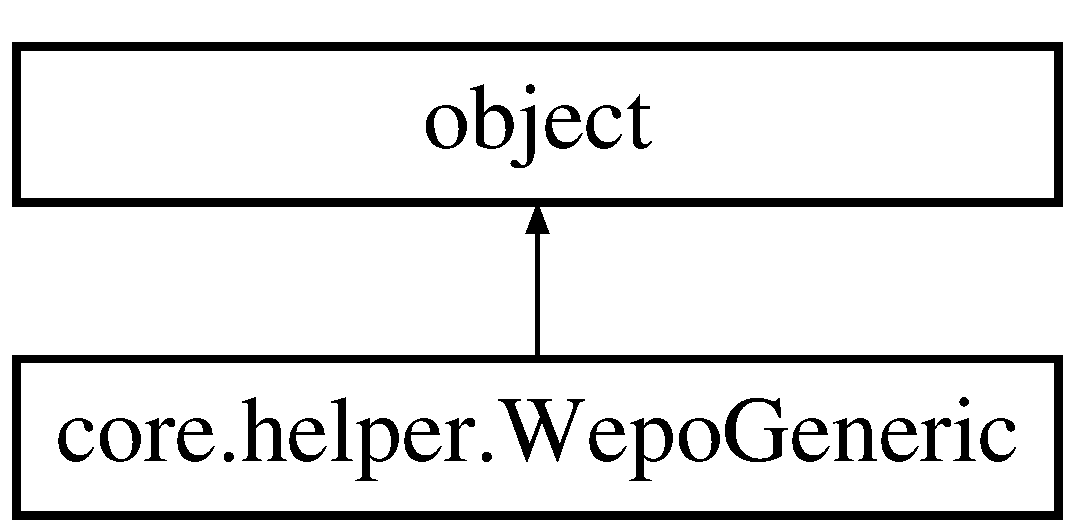
\includegraphics[height=2.000000cm]{classcore_1_1helper_1_1WepoGeneric}
\end{center}
\end{figure}
\subsection*{Public Member Functions}
\begin{DoxyCompactItemize}
\item 
def \hyperlink{classcore_1_1helper_1_1WepoGeneric_a83ef1df0334c5cc72ea89fa029cc37c4}{\-\_\-\-\_\-init\-\_\-\-\_\-}
\item 
def \hyperlink{classcore_1_1helper_1_1WepoGeneric_a2072481aaf051287e56ed4dfd87ffec7}{\-\_\-\-\_\-getitem\-\_\-\-\_\-}
\item 
def \hyperlink{classcore_1_1helper_1_1WepoGeneric_abfdf3390194b505fd0c05361b3c83564}{\-\_\-\-\_\-setitem\-\_\-\-\_\-}
\item 
def \hyperlink{classcore_1_1helper_1_1WepoGeneric_af1d485ced44f07dc3998efdbe2dce657}{\-\_\-\-\_\-delitem\-\_\-\-\_\-}
\item 
def \hyperlink{classcore_1_1helper_1_1WepoGeneric_a6ac9090db2617973fdd72e70cddf47e0}{\-\_\-\-\_\-contains\-\_\-\-\_\-}
\item 
def \hyperlink{classcore_1_1helper_1_1WepoGeneric_ab2a4b8ebc9e566c288ccdbc3f4091c0f}{\-\_\-\-\_\-len\-\_\-\-\_\-}
\item 
def \hyperlink{classcore_1_1helper_1_1WepoGeneric_a9899aa93968cea184da6e68e7008f0f5}{\-\_\-\-\_\-repr\-\_\-\-\_\-}
\item 
def \hyperlink{classcore_1_1helper_1_1WepoGeneric_a3f655e187e647683b5209ac4df0341de}{default}
\item 
def \hyperlink{classcore_1_1helper_1_1WepoGeneric_a88d3712b75a9e33a30488686ac4a5737}{get}
\item 
def \hyperlink{classcore_1_1helper_1_1WepoGeneric_ac639a89dd3376ad018d3063d53e256e5}{items}
\end{DoxyCompactItemize}


\subsection{Detailed Description}
Generic class for dictionary parsed to object. 

\subsection{Constructor \& Destructor Documentation}
\hypertarget{classcore_1_1helper_1_1WepoGeneric_a83ef1df0334c5cc72ea89fa029cc37c4}{\index{core\-::helper\-::\-Wepo\-Generic@{core\-::helper\-::\-Wepo\-Generic}!\-\_\-\-\_\-init\-\_\-\-\_\-@{\-\_\-\-\_\-init\-\_\-\-\_\-}}
\index{\-\_\-\-\_\-init\-\_\-\-\_\-@{\-\_\-\-\_\-init\-\_\-\-\_\-}!core::helper::WepoGeneric@{core\-::helper\-::\-Wepo\-Generic}}
\subsubsection[{\-\_\-\-\_\-init\-\_\-\-\_\-}]{\setlength{\rightskip}{0pt plus 5cm}def core.\-helper.\-Wepo\-Generic.\-\_\-\-\_\-init\-\_\-\-\_\- (
\begin{DoxyParamCaption}
\item[{}]{self, }
\item[{}]{init = {\ttfamily None}}
\end{DoxyParamCaption}
)}}\label{classcore_1_1helper_1_1WepoGeneric_a83ef1df0334c5cc72ea89fa029cc37c4}


\subsection{Member Function Documentation}
\hypertarget{classcore_1_1helper_1_1WepoGeneric_a6ac9090db2617973fdd72e70cddf47e0}{\index{core\-::helper\-::\-Wepo\-Generic@{core\-::helper\-::\-Wepo\-Generic}!\-\_\-\-\_\-contains\-\_\-\-\_\-@{\-\_\-\-\_\-contains\-\_\-\-\_\-}}
\index{\-\_\-\-\_\-contains\-\_\-\-\_\-@{\-\_\-\-\_\-contains\-\_\-\-\_\-}!core::helper::WepoGeneric@{core\-::helper\-::\-Wepo\-Generic}}
\subsubsection[{\-\_\-\-\_\-contains\-\_\-\-\_\-}]{\setlength{\rightskip}{0pt plus 5cm}def core.\-helper.\-Wepo\-Generic.\-\_\-\-\_\-contains\-\_\-\-\_\- (
\begin{DoxyParamCaption}
\item[{}]{self, }
\item[{}]{key}
\end{DoxyParamCaption}
)}}\label{classcore_1_1helper_1_1WepoGeneric_a6ac9090db2617973fdd72e70cddf47e0}
\hypertarget{classcore_1_1helper_1_1WepoGeneric_af1d485ced44f07dc3998efdbe2dce657}{\index{core\-::helper\-::\-Wepo\-Generic@{core\-::helper\-::\-Wepo\-Generic}!\-\_\-\-\_\-delitem\-\_\-\-\_\-@{\-\_\-\-\_\-delitem\-\_\-\-\_\-}}
\index{\-\_\-\-\_\-delitem\-\_\-\-\_\-@{\-\_\-\-\_\-delitem\-\_\-\-\_\-}!core::helper::WepoGeneric@{core\-::helper\-::\-Wepo\-Generic}}
\subsubsection[{\-\_\-\-\_\-delitem\-\_\-\-\_\-}]{\setlength{\rightskip}{0pt plus 5cm}def core.\-helper.\-Wepo\-Generic.\-\_\-\-\_\-delitem\-\_\-\-\_\- (
\begin{DoxyParamCaption}
\item[{}]{self, }
\item[{}]{key}
\end{DoxyParamCaption}
)}}\label{classcore_1_1helper_1_1WepoGeneric_af1d485ced44f07dc3998efdbe2dce657}
\hypertarget{classcore_1_1helper_1_1WepoGeneric_a2072481aaf051287e56ed4dfd87ffec7}{\index{core\-::helper\-::\-Wepo\-Generic@{core\-::helper\-::\-Wepo\-Generic}!\-\_\-\-\_\-getitem\-\_\-\-\_\-@{\-\_\-\-\_\-getitem\-\_\-\-\_\-}}
\index{\-\_\-\-\_\-getitem\-\_\-\-\_\-@{\-\_\-\-\_\-getitem\-\_\-\-\_\-}!core::helper::WepoGeneric@{core\-::helper\-::\-Wepo\-Generic}}
\subsubsection[{\-\_\-\-\_\-getitem\-\_\-\-\_\-}]{\setlength{\rightskip}{0pt plus 5cm}def core.\-helper.\-Wepo\-Generic.\-\_\-\-\_\-getitem\-\_\-\-\_\- (
\begin{DoxyParamCaption}
\item[{}]{self, }
\item[{}]{key}
\end{DoxyParamCaption}
)}}\label{classcore_1_1helper_1_1WepoGeneric_a2072481aaf051287e56ed4dfd87ffec7}
\hypertarget{classcore_1_1helper_1_1WepoGeneric_ab2a4b8ebc9e566c288ccdbc3f4091c0f}{\index{core\-::helper\-::\-Wepo\-Generic@{core\-::helper\-::\-Wepo\-Generic}!\-\_\-\-\_\-len\-\_\-\-\_\-@{\-\_\-\-\_\-len\-\_\-\-\_\-}}
\index{\-\_\-\-\_\-len\-\_\-\-\_\-@{\-\_\-\-\_\-len\-\_\-\-\_\-}!core::helper::WepoGeneric@{core\-::helper\-::\-Wepo\-Generic}}
\subsubsection[{\-\_\-\-\_\-len\-\_\-\-\_\-}]{\setlength{\rightskip}{0pt plus 5cm}def core.\-helper.\-Wepo\-Generic.\-\_\-\-\_\-len\-\_\-\-\_\- (
\begin{DoxyParamCaption}
\item[{}]{self}
\end{DoxyParamCaption}
)}}\label{classcore_1_1helper_1_1WepoGeneric_ab2a4b8ebc9e566c288ccdbc3f4091c0f}
\hypertarget{classcore_1_1helper_1_1WepoGeneric_a9899aa93968cea184da6e68e7008f0f5}{\index{core\-::helper\-::\-Wepo\-Generic@{core\-::helper\-::\-Wepo\-Generic}!\-\_\-\-\_\-repr\-\_\-\-\_\-@{\-\_\-\-\_\-repr\-\_\-\-\_\-}}
\index{\-\_\-\-\_\-repr\-\_\-\-\_\-@{\-\_\-\-\_\-repr\-\_\-\-\_\-}!core::helper::WepoGeneric@{core\-::helper\-::\-Wepo\-Generic}}
\subsubsection[{\-\_\-\-\_\-repr\-\_\-\-\_\-}]{\setlength{\rightskip}{0pt plus 5cm}def core.\-helper.\-Wepo\-Generic.\-\_\-\-\_\-repr\-\_\-\-\_\- (
\begin{DoxyParamCaption}
\item[{}]{self}
\end{DoxyParamCaption}
)}}\label{classcore_1_1helper_1_1WepoGeneric_a9899aa93968cea184da6e68e7008f0f5}
\hypertarget{classcore_1_1helper_1_1WepoGeneric_abfdf3390194b505fd0c05361b3c83564}{\index{core\-::helper\-::\-Wepo\-Generic@{core\-::helper\-::\-Wepo\-Generic}!\-\_\-\-\_\-setitem\-\_\-\-\_\-@{\-\_\-\-\_\-setitem\-\_\-\-\_\-}}
\index{\-\_\-\-\_\-setitem\-\_\-\-\_\-@{\-\_\-\-\_\-setitem\-\_\-\-\_\-}!core::helper::WepoGeneric@{core\-::helper\-::\-Wepo\-Generic}}
\subsubsection[{\-\_\-\-\_\-setitem\-\_\-\-\_\-}]{\setlength{\rightskip}{0pt plus 5cm}def core.\-helper.\-Wepo\-Generic.\-\_\-\-\_\-setitem\-\_\-\-\_\- (
\begin{DoxyParamCaption}
\item[{}]{self, }
\item[{}]{key, }
\item[{}]{value}
\end{DoxyParamCaption}
)}}\label{classcore_1_1helper_1_1WepoGeneric_abfdf3390194b505fd0c05361b3c83564}
\hypertarget{classcore_1_1helper_1_1WepoGeneric_a3f655e187e647683b5209ac4df0341de}{\index{core\-::helper\-::\-Wepo\-Generic@{core\-::helper\-::\-Wepo\-Generic}!default@{default}}
\index{default@{default}!core::helper::WepoGeneric@{core\-::helper\-::\-Wepo\-Generic}}
\subsubsection[{default}]{\setlength{\rightskip}{0pt plus 5cm}def core.\-helper.\-Wepo\-Generic.\-default (
\begin{DoxyParamCaption}
\item[{}]{self}
\end{DoxyParamCaption}
)}}\label{classcore_1_1helper_1_1WepoGeneric_a3f655e187e647683b5209ac4df0341de}
\hypertarget{classcore_1_1helper_1_1WepoGeneric_a88d3712b75a9e33a30488686ac4a5737}{\index{core\-::helper\-::\-Wepo\-Generic@{core\-::helper\-::\-Wepo\-Generic}!get@{get}}
\index{get@{get}!core::helper::WepoGeneric@{core\-::helper\-::\-Wepo\-Generic}}
\subsubsection[{get}]{\setlength{\rightskip}{0pt plus 5cm}def core.\-helper.\-Wepo\-Generic.\-get (
\begin{DoxyParamCaption}
\item[{}]{self, }
\item[{}]{key, }
\item[{}]{default}
\end{DoxyParamCaption}
)}}\label{classcore_1_1helper_1_1WepoGeneric_a88d3712b75a9e33a30488686ac4a5737}
\hypertarget{classcore_1_1helper_1_1WepoGeneric_ac639a89dd3376ad018d3063d53e256e5}{\index{core\-::helper\-::\-Wepo\-Generic@{core\-::helper\-::\-Wepo\-Generic}!items@{items}}
\index{items@{items}!core::helper::WepoGeneric@{core\-::helper\-::\-Wepo\-Generic}}
\subsubsection[{items}]{\setlength{\rightskip}{0pt plus 5cm}def core.\-helper.\-Wepo\-Generic.\-items (
\begin{DoxyParamCaption}
\item[{}]{self}
\end{DoxyParamCaption}
)}}\label{classcore_1_1helper_1_1WepoGeneric_ac639a89dd3376ad018d3063d53e256e5}


The documentation for this class was generated from the following file\-:\begin{DoxyCompactItemize}
\item 
/wepo/core/helper/\hyperlink{core_2helper_2____init_____8py}{\-\_\-\-\_\-init\-\_\-\-\_\-.\-py}\end{DoxyCompactItemize}

\chapter{File Documentation}
\hypertarget{apps_2____init_____8py}{\section{/wepo/apps/\-\_\-\-\_\-init\-\_\-\-\_\-.py File Reference}
\label{apps_2____init_____8py}\index{/wepo/apps/\-\_\-\-\_\-init\-\_\-\-\_\-.\-py@{/wepo/apps/\-\_\-\-\_\-init\-\_\-\-\_\-.\-py}}
}
\subsection*{Namespaces}
\begin{DoxyCompactItemize}
\item 
\hyperlink{namespaceapps}{apps}
\end{DoxyCompactItemize}

\hypertarget{core_2____init_____8py}{\section{/wepo/core/\-\_\-\-\_\-init\-\_\-\-\_\-.py File Reference}
\label{core_2____init_____8py}\index{/wepo/core/\-\_\-\-\_\-init\-\_\-\-\_\-.\-py@{/wepo/core/\-\_\-\-\_\-init\-\_\-\-\_\-.\-py}}
}
\subsection*{Namespaces}
\begin{DoxyCompactItemize}
\item 
\hyperlink{namespacecore}{core}
\end{DoxyCompactItemize}
\subsection*{Variables}
\begin{DoxyCompactItemize}
\item 
tuple \hyperlink{namespacecore_aa3a4d9b7cefbd434631d48e879351f8d}{core.\-wepo\-\_\-assets} = Wepo\-Generic()
\end{DoxyCompactItemize}

\hypertarget{core_2blocks_2____init_____8py}{\section{/wepo/core/blocks/\-\_\-\-\_\-init\-\_\-\-\_\-.py File Reference}
\label{core_2blocks_2____init_____8py}\index{/wepo/core/blocks/\-\_\-\-\_\-init\-\_\-\-\_\-.\-py@{/wepo/core/blocks/\-\_\-\-\_\-init\-\_\-\-\_\-.\-py}}
}
\subsection*{Namespaces}
\begin{DoxyCompactItemize}
\item 
\hyperlink{namespacecore_1_1blocks}{core.\-blocks}
\end{DoxyCompactItemize}
\subsection*{Variables}
\begin{DoxyCompactItemize}
\item 
string \hyperlink{namespacecore_1_1blocks_acb90e6c6865546d6a3b69b8fb2abfae3}{core.\-blocks.\-\_\-\-\_\-author\-\_\-\-\_\-} = 'timrc'
\end{DoxyCompactItemize}

\hypertarget{core_2blocks_2admin_2____init_____8py}{\section{/wepo/core/blocks/admin/\-\_\-\-\_\-init\-\_\-\-\_\-.py File Reference}
\label{core_2blocks_2admin_2____init_____8py}\index{/wepo/core/blocks/admin/\-\_\-\-\_\-init\-\_\-\-\_\-.\-py@{/wepo/core/blocks/admin/\-\_\-\-\_\-init\-\_\-\-\_\-.\-py}}
}
\subsection*{Namespaces}
\begin{DoxyCompactItemize}
\item 
\hyperlink{namespacecore_1_1blocks_1_1admin}{core.\-blocks.\-admin}
\end{DoxyCompactItemize}
\subsection*{Variables}
\begin{DoxyCompactItemize}
\item 
string \hyperlink{namespacecore_1_1blocks_1_1admin_aadde964b15b9d7a4abde5732c061ab23}{core.\-blocks.\-admin.\-\_\-\-\_\-author\-\_\-\-\_\-} = 'timrc'
\end{DoxyCompactItemize}

\hypertarget{core_2decorators_2____init_____8py}{\section{/wepo/core/decorators/\-\_\-\-\_\-init\-\_\-\-\_\-.py File Reference}
\label{core_2decorators_2____init_____8py}\index{/wepo/core/decorators/\-\_\-\-\_\-init\-\_\-\-\_\-.\-py@{/wepo/core/decorators/\-\_\-\-\_\-init\-\_\-\-\_\-.\-py}}
}
\subsection*{Namespaces}
\begin{DoxyCompactItemize}
\item 
\hyperlink{namespacecore_1_1decorators}{core.\-decorators}
\end{DoxyCompactItemize}

\hypertarget{core_2form_2____init_____8py}{\section{/wepo/core/form/\-\_\-\-\_\-init\-\_\-\-\_\-.py File Reference}
\label{core_2form_2____init_____8py}\index{/wepo/core/form/\-\_\-\-\_\-init\-\_\-\-\_\-.\-py@{/wepo/core/form/\-\_\-\-\_\-init\-\_\-\-\_\-.\-py}}
}
\subsection*{Classes}
\begin{DoxyCompactItemize}
\item 
class \hyperlink{classcore_1_1form_1_1Form}{core.\-form.\-Form}
\begin{DoxyCompactList}\small\item\em Wepo form class. \end{DoxyCompactList}\item 
class \hyperlink{classcore_1_1form_1_1FormGroup}{core.\-form.\-Form\-Group}
\begin{DoxyCompactList}\small\item\em Wepo form field sets class. \end{DoxyCompactList}\item 
class \hyperlink{classcore_1_1form_1_1FormItem}{core.\-form.\-Form\-Item}
\begin{DoxyCompactList}\small\item\em Wepo form item class. \end{DoxyCompactList}\end{DoxyCompactItemize}
\subsection*{Namespaces}
\begin{DoxyCompactItemize}
\item 
\hyperlink{namespacecore_1_1form}{core.\-form}
\end{DoxyCompactItemize}
\subsection*{Functions}
\begin{DoxyCompactItemize}
\item 
def \hyperlink{namespacecore_1_1form_aafa98fa8aa06421679f6f115265ba02a}{core.\-form.\-get\-\_\-form\-\_\-items}
\begin{DoxyCompactList}\small\item\em Get form items from installed apps. \end{DoxyCompactList}\end{DoxyCompactItemize}

\hypertarget{core_2form_2elements_2____init_____8py}{\section{/wepo/core/form/elements/\-\_\-\-\_\-init\-\_\-\-\_\-.py File Reference}
\label{core_2form_2elements_2____init_____8py}\index{/wepo/core/form/elements/\-\_\-\-\_\-init\-\_\-\-\_\-.\-py@{/wepo/core/form/elements/\-\_\-\-\_\-init\-\_\-\-\_\-.\-py}}
}
\subsection*{Namespaces}
\begin{DoxyCompactItemize}
\item 
\hyperlink{namespacecore_1_1form_1_1elements}{core.\-form.\-elements}
\end{DoxyCompactItemize}

\hypertarget{core_2helper_2____init_____8py}{\section{/wepo/core/helper/\-\_\-\-\_\-init\-\_\-\-\_\-.py File Reference}
\label{core_2helper_2____init_____8py}\index{/wepo/core/helper/\-\_\-\-\_\-init\-\_\-\-\_\-.\-py@{/wepo/core/helper/\-\_\-\-\_\-init\-\_\-\-\_\-.\-py}}
}
\subsection*{Classes}
\begin{DoxyCompactItemize}
\item 
class \hyperlink{classcore_1_1helper_1_1WepoGeneric}{core.\-helper.\-Wepo\-Generic}
\begin{DoxyCompactList}\small\item\em Generic class for dictionary parsed to object. \end{DoxyCompactList}\end{DoxyCompactItemize}
\subsection*{Namespaces}
\begin{DoxyCompactItemize}
\item 
\hyperlink{namespacecore_1_1helper}{core.\-helper}
\end{DoxyCompactItemize}
\subsection*{Functions}
\begin{DoxyCompactItemize}
\item 
def \hyperlink{namespacecore_1_1helper_af4bbf3a391a72499c5840c42ced86051}{core.\-helper.\-get\-\_\-request}
\begin{DoxyCompactList}\small\item\em Global get request helper. \end{DoxyCompactList}\item 
def \hyperlink{namespacecore_1_1helper_a75fc1f2204d7ac3c6090b9cf854c842a}{core.\-helper.\-dict\-\_\-to\-\_\-obj}
\begin{DoxyCompactList}\small\item\em Dictionary to object (json to object) etc. \end{DoxyCompactList}\item 
def \hyperlink{namespacecore_1_1helper_aca3430be2ff434d731113002ae90e432}{core.\-helper.\-dict\-\_\-list\-\_\-to\-\_\-obj}
\begin{DoxyCompactList}\small\item\em List of dictionaries to list of objects (json to object) etc. \end{DoxyCompactList}\item 
def \hyperlink{namespacecore_1_1helper_aea7e9831df34936caaeacc9a1498ad70}{core.\-helper.\-add\-\_\-dict\-\_\-to\-\_\-object}
\begin{DoxyCompactList}\small\item\em Update object attributes with given dictionary. \end{DoxyCompactList}\item 
def \hyperlink{namespacecore_1_1helper_ab3aae413c3bf9c912dd52c22f46cab19}{core.\-helper.\-add\-\_\-to\-\_\-request}
\begin{DoxyCompactList}\small\item\em Add/update object to wepo request. \end{DoxyCompactList}\item 
def \hyperlink{namespacecore_1_1helper_a0646d87e47a6af56a82f5fc3085bee55}{core.\-helper.\-build\-\_\-url}
\begin{DoxyCompactList}\small\item\em Build url from list. \end{DoxyCompactList}\item 
def \hyperlink{namespacecore_1_1helper_a531241dec617f00663b073544cb98eb8}{core.\-helper.\-get\-\_\-module}
\begin{DoxyCompactList}\small\item\em Get module from the path. \end{DoxyCompactList}\item 
def \hyperlink{namespacecore_1_1helper_a583a27b0826faf86c974661a2319c710}{core.\-helper.\-get\-\_\-function}
\begin{DoxyCompactList}\small\item\em Get function from the module. \end{DoxyCompactList}\item 
def \hyperlink{namespacecore_1_1helper_a074ccfdd66dd5986d0d507e38bee2d42}{core.\-helper.\-get\-\_\-layout\-\_\-config}
\begin{DoxyCompactList}\small\item\em Get layout config from request. \end{DoxyCompactList}\item 
def \hyperlink{namespacecore_1_1helper_a182e0063dd07af986372778830858d3b}{core.\-helper.\-get\-\_\-page\-\_\-layout\-\_\-config}
\begin{DoxyCompactList}\small\item\em Get layout config from request. \end{DoxyCompactList}\item 
def \hyperlink{namespacecore_1_1helper_ac438e0067a81450db9762d52c0636a4a}{core.\-helper.\-get\-\_\-page\-\_\-sections}
\begin{DoxyCompactList}\small\item\em Get page layout sections. \end{DoxyCompactList}\item 
def \hyperlink{namespacecore_1_1helper_a8ea9bf0f6bf426a11ca63a9b92d72080}{core.\-helper.\-get\-\_\-layouts}
\begin{DoxyCompactList}\small\item\em Get layouts from installed apps. \end{DoxyCompactList}\end{DoxyCompactItemize}

\hypertarget{core_2install_2____init_____8py}{\section{/wepo/core/install/\-\_\-\-\_\-init\-\_\-\-\_\-.py File Reference}
\label{core_2install_2____init_____8py}\index{/wepo/core/install/\-\_\-\-\_\-init\-\_\-\-\_\-.\-py@{/wepo/core/install/\-\_\-\-\_\-init\-\_\-\-\_\-.\-py}}
}
\subsection*{Classes}
\begin{DoxyCompactItemize}
\item 
class \hyperlink{classcore_1_1install_1_1Install}{core.\-install.\-Install}
\begin{DoxyCompactList}\small\item\em \hyperlink{classcore_1_1install_1_1Install}{Install} objects. \end{DoxyCompactList}\end{DoxyCompactItemize}
\subsection*{Namespaces}
\begin{DoxyCompactItemize}
\item 
\hyperlink{namespacecore_1_1install}{core.\-install}
\end{DoxyCompactItemize}

\hypertarget{core_2management_2____init_____8py}{\section{/wepo/core/management/\-\_\-\-\_\-init\-\_\-\-\_\-.py File Reference}
\label{core_2management_2____init_____8py}\index{/wepo/core/management/\-\_\-\-\_\-init\-\_\-\-\_\-.\-py@{/wepo/core/management/\-\_\-\-\_\-init\-\_\-\-\_\-.\-py}}
}
\subsection*{Namespaces}
\begin{DoxyCompactItemize}
\item 
\hyperlink{namespacecore_1_1management}{core.\-management}
\end{DoxyCompactItemize}
\subsection*{Variables}
\begin{DoxyCompactItemize}
\item 
string \hyperlink{namespacecore_1_1management_ae3082b96220121385ce826286ade727a}{core.\-management.\-\_\-\-\_\-author\-\_\-\-\_\-} = 'timrc'
\end{DoxyCompactItemize}

\hypertarget{core_2management_2commands_2____init_____8py}{\section{/wepo/core/management/commands/\-\_\-\-\_\-init\-\_\-\-\_\-.py File Reference}
\label{core_2management_2commands_2____init_____8py}\index{/wepo/core/management/commands/\-\_\-\-\_\-init\-\_\-\-\_\-.\-py@{/wepo/core/management/commands/\-\_\-\-\_\-init\-\_\-\-\_\-.\-py}}
}
\subsection*{Namespaces}
\begin{DoxyCompactItemize}
\item 
\hyperlink{namespacecore_1_1management_1_1commands}{core.\-management.\-commands}
\end{DoxyCompactItemize}
\subsection*{Variables}
\begin{DoxyCompactItemize}
\item 
string \hyperlink{namespacecore_1_1management_1_1commands_ac1c6651c8c0dfcb25f81696c4889951a}{core.\-management.\-commands.\-\_\-\-\_\-author\-\_\-\-\_\-} = 'timrc'
\end{DoxyCompactItemize}

\hypertarget{core_2middleware_2____init_____8py}{\section{/wepo/core/middleware/\-\_\-\-\_\-init\-\_\-\-\_\-.py File Reference}
\label{core_2middleware_2____init_____8py}\index{/wepo/core/middleware/\-\_\-\-\_\-init\-\_\-\-\_\-.\-py@{/wepo/core/middleware/\-\_\-\-\_\-init\-\_\-\-\_\-.\-py}}
}
\subsection*{Classes}
\begin{DoxyCompactItemize}
\item 
class \hyperlink{classcore_1_1middleware_1_1GlobalRequest}{core.\-middleware.\-Global\-Request}
\begin{DoxyCompactList}\small\item\em Thread-\/safe middleware that makes the current request object available globally. \end{DoxyCompactList}\end{DoxyCompactItemize}
\subsection*{Namespaces}
\begin{DoxyCompactItemize}
\item 
\hyperlink{namespacecore_1_1middleware}{core.\-middleware}
\end{DoxyCompactItemize}

\hypertarget{core_2permissions_2____init_____8py}{\section{/wepo/core/permissions/\-\_\-\-\_\-init\-\_\-\-\_\-.py File Reference}
\label{core_2permissions_2____init_____8py}\index{/wepo/core/permissions/\-\_\-\-\_\-init\-\_\-\-\_\-.\-py@{/wepo/core/permissions/\-\_\-\-\_\-init\-\_\-\-\_\-.\-py}}
}
\subsection*{Namespaces}
\begin{DoxyCompactItemize}
\item 
\hyperlink{namespacecore_1_1permissions}{core.\-permissions}
\end{DoxyCompactItemize}

\hypertarget{core_2permissions_2admin_2____init_____8py}{\section{/wepo/core/permissions/admin/\-\_\-\-\_\-init\-\_\-\-\_\-.py File Reference}
\label{core_2permissions_2admin_2____init_____8py}\index{/wepo/core/permissions/admin/\-\_\-\-\_\-init\-\_\-\-\_\-.\-py@{/wepo/core/permissions/admin/\-\_\-\-\_\-init\-\_\-\-\_\-.\-py}}
}
\subsection*{Namespaces}
\begin{DoxyCompactItemize}
\item 
\hyperlink{namespacecore_1_1permissions_1_1admin}{core.\-permissions.\-admin}
\end{DoxyCompactItemize}
\subsection*{Functions}
\begin{DoxyCompactItemize}
\item 
def \hyperlink{namespacecore_1_1permissions_1_1admin_a028d910c4043f285b4fa39d88a6626e2}{core.\-permissions.\-admin.\-admin\-\_\-access}
\begin{DoxyCompactList}\small\item\em Administration permission callback. \end{DoxyCompactList}\end{DoxyCompactItemize}

\hypertarget{core_2permissions_2user_2____init_____8py}{\section{/wepo/core/permissions/user/\-\_\-\-\_\-init\-\_\-\-\_\-.py File Reference}
\label{core_2permissions_2user_2____init_____8py}\index{/wepo/core/permissions/user/\-\_\-\-\_\-init\-\_\-\-\_\-.\-py@{/wepo/core/permissions/user/\-\_\-\-\_\-init\-\_\-\-\_\-.\-py}}
}
\subsection*{Namespaces}
\begin{DoxyCompactItemize}
\item 
\hyperlink{namespacecore_1_1permissions_1_1user}{core.\-permissions.\-user}
\end{DoxyCompactItemize}
\subsection*{Functions}
\begin{DoxyCompactItemize}
\item 
def \hyperlink{namespacecore_1_1permissions_1_1user_ae3e347fb35459d4c94b2545527899fce}{core.\-permissions.\-user.\-authenticated}
\begin{DoxyCompactList}\small\item\em Administration permission callback. \end{DoxyCompactList}\end{DoxyCompactItemize}

\hypertarget{core_2templates_2____init_____8py}{\section{/wepo/core/templates/\-\_\-\-\_\-init\-\_\-\-\_\-.py File Reference}
\label{core_2templates_2____init_____8py}\index{/wepo/core/templates/\-\_\-\-\_\-init\-\_\-\-\_\-.\-py@{/wepo/core/templates/\-\_\-\-\_\-init\-\_\-\-\_\-.\-py}}
}
\subsection*{Namespaces}
\begin{DoxyCompactItemize}
\item 
\hyperlink{namespacecore_1_1templates}{core.\-templates}
\end{DoxyCompactItemize}

\hypertarget{core_2templates_2admin_2____init_____8py}{\section{/wepo/core/templates/admin/\-\_\-\-\_\-init\-\_\-\-\_\-.py File Reference}
\label{core_2templates_2admin_2____init_____8py}\index{/wepo/core/templates/admin/\-\_\-\-\_\-init\-\_\-\-\_\-.\-py@{/wepo/core/templates/admin/\-\_\-\-\_\-init\-\_\-\-\_\-.\-py}}
}
\subsection*{Namespaces}
\begin{DoxyCompactItemize}
\item 
\hyperlink{namespacecore_1_1templates_1_1admin}{core.\-templates.\-admin}
\end{DoxyCompactItemize}

\hypertarget{core_2templates_2layout_2____init_____8py}{\section{/wepo/core/templates/layout/\-\_\-\-\_\-init\-\_\-\-\_\-.py File Reference}
\label{core_2templates_2layout_2____init_____8py}\index{/wepo/core/templates/layout/\-\_\-\-\_\-init\-\_\-\-\_\-.\-py@{/wepo/core/templates/layout/\-\_\-\-\_\-init\-\_\-\-\_\-.\-py}}
}
\subsection*{Namespaces}
\begin{DoxyCompactItemize}
\item 
\hyperlink{namespacecore_1_1templates_1_1layout}{core.\-templates.\-layout}
\end{DoxyCompactItemize}

\hypertarget{core_2templates_2layout_2admin_2____init_____8py}{\section{/wepo/core/templates/layout/admin/\-\_\-\-\_\-init\-\_\-\-\_\-.py File Reference}
\label{core_2templates_2layout_2admin_2____init_____8py}\index{/wepo/core/templates/layout/admin/\-\_\-\-\_\-init\-\_\-\-\_\-.\-py@{/wepo/core/templates/layout/admin/\-\_\-\-\_\-init\-\_\-\-\_\-.\-py}}
}
\subsection*{Namespaces}
\begin{DoxyCompactItemize}
\item 
\hyperlink{namespacecore_1_1templates_1_1layout_1_1admin}{core.\-templates.\-layout.\-admin}
\end{DoxyCompactItemize}
\subsection*{Variables}
\begin{DoxyCompactItemize}
\item 
string \hyperlink{namespacecore_1_1templates_1_1layout_1_1admin_af7d38b988955e21e8245afa44686ce60}{core.\-templates.\-layout.\-admin.\-name} = 'Admin layout'
\end{DoxyCompactItemize}

\hypertarget{core_2templates_2layout_2admin_2empty_2____init_____8py}{\section{/wepo/core/templates/layout/admin/empty/\-\_\-\-\_\-init\-\_\-\-\_\-.py File Reference}
\label{core_2templates_2layout_2admin_2empty_2____init_____8py}\index{/wepo/core/templates/layout/admin/empty/\-\_\-\-\_\-init\-\_\-\-\_\-.\-py@{/wepo/core/templates/layout/admin/empty/\-\_\-\-\_\-init\-\_\-\-\_\-.\-py}}
}
\subsection*{Namespaces}
\begin{DoxyCompactItemize}
\item 
\hyperlink{namespacecore_1_1templates_1_1layout_1_1admin_1_1empty}{core.\-templates.\-layout.\-admin.\-empty}
\end{DoxyCompactItemize}
\subsection*{Variables}
\begin{DoxyCompactItemize}
\item 
string \hyperlink{namespacecore_1_1templates_1_1layout_1_1admin_1_1empty_a6b6dee13512e187e08c8f71c5f63cd64}{core.\-templates.\-layout.\-admin.\-empty.\-name} = 'Admin empty layout'
\end{DoxyCompactItemize}

\hypertarget{core_2templates_2layout_2empty_2____init_____8py}{\section{/wepo/core/templates/layout/empty/\-\_\-\-\_\-init\-\_\-\-\_\-.py File Reference}
\label{core_2templates_2layout_2empty_2____init_____8py}\index{/wepo/core/templates/layout/empty/\-\_\-\-\_\-init\-\_\-\-\_\-.\-py@{/wepo/core/templates/layout/empty/\-\_\-\-\_\-init\-\_\-\-\_\-.\-py}}
}
\subsection*{Namespaces}
\begin{DoxyCompactItemize}
\item 
\hyperlink{namespacecore_1_1templates_1_1layout_1_1empty}{core.\-templates.\-layout.\-empty}
\end{DoxyCompactItemize}
\subsection*{Variables}
\begin{DoxyCompactItemize}
\item 
string \hyperlink{namespacecore_1_1templates_1_1layout_1_1empty_a8dbeb9bbaeff8ee7a6d40873fdbf81cc}{core.\-templates.\-layout.\-empty.\-name} = 'Empty layout'
\end{DoxyCompactItemize}

\hypertarget{core_2templatetags_2____init_____8py}{\section{/wepo/core/templatetags/\-\_\-\-\_\-init\-\_\-\-\_\-.py File Reference}
\label{core_2templatetags_2____init_____8py}\index{/wepo/core/templatetags/\-\_\-\-\_\-init\-\_\-\-\_\-.\-py@{/wepo/core/templatetags/\-\_\-\-\_\-init\-\_\-\-\_\-.\-py}}
}
\subsection*{Namespaces}
\begin{DoxyCompactItemize}
\item 
\hyperlink{namespacecore_1_1templatetags}{core.\-templatetags}
\end{DoxyCompactItemize}

\hypertarget{core_2unit_2____init_____8py}{\section{/wepo/core/unit/\-\_\-\-\_\-init\-\_\-\-\_\-.py File Reference}
\label{core_2unit_2____init_____8py}\index{/wepo/core/unit/\-\_\-\-\_\-init\-\_\-\-\_\-.\-py@{/wepo/core/unit/\-\_\-\-\_\-init\-\_\-\-\_\-.\-py}}
}
\subsection*{Namespaces}
\begin{DoxyCompactItemize}
\item 
\hyperlink{namespacecore_1_1unit}{core.\-unit}
\end{DoxyCompactItemize}
\subsection*{Variables}
\begin{DoxyCompactItemize}
\item 
string \hyperlink{namespacecore_1_1unit_a19dc25223605b84c46ac5ef96a183229}{core.\-unit.\-\_\-\-\_\-author\-\_\-\-\_\-} = 'timrc'
\end{DoxyCompactItemize}

\hypertarget{overrides_2____init_____8py}{\section{/wepo/overrides/\-\_\-\-\_\-init\-\_\-\-\_\-.py File Reference}
\label{overrides_2____init_____8py}\index{/wepo/overrides/\-\_\-\-\_\-init\-\_\-\-\_\-.\-py@{/wepo/overrides/\-\_\-\-\_\-init\-\_\-\-\_\-.\-py}}
}
\subsection*{Namespaces}
\begin{DoxyCompactItemize}
\item 
\hyperlink{namespaceoverrides}{overrides}
\end{DoxyCompactItemize}

\hypertarget{wepo_2____init_____8py}{\section{/wepo/wepo/\-\_\-\-\_\-init\-\_\-\-\_\-.py File Reference}
\label{wepo_2____init_____8py}\index{/wepo/wepo/\-\_\-\-\_\-init\-\_\-\-\_\-.\-py@{/wepo/wepo/\-\_\-\-\_\-init\-\_\-\-\_\-.\-py}}
}
\subsection*{Namespaces}
\begin{DoxyCompactItemize}
\item 
\hyperlink{namespacewepo}{wepo}
\end{DoxyCompactItemize}

\hypertarget{ajax_8py}{\section{/wepo/core/ajax.py File Reference}
\label{ajax_8py}\index{/wepo/core/ajax.\-py@{/wepo/core/ajax.\-py}}
}
\subsection*{Namespaces}
\begin{DoxyCompactItemize}
\item 
\hyperlink{namespacecore_1_1ajax}{core.\-ajax}
\end{DoxyCompactItemize}
\subsection*{Functions}
\begin{DoxyCompactItemize}
\item 
def \hyperlink{namespacecore_1_1ajax_a0946391b6ef7c6a31cf33ce1dd6fb3af}{core.\-ajax.\-invoke\-\_\-callback}
\begin{DoxyCompactList}\small\item\em Invoke called callback. \end{DoxyCompactList}\end{DoxyCompactItemize}

\hypertarget{asset_8py}{\section{/wepo/core/asset.py File Reference}
\label{asset_8py}\index{/wepo/core/asset.\-py@{/wepo/core/asset.\-py}}
}
\subsection*{Namespaces}
\begin{DoxyCompactItemize}
\item 
\hyperlink{namespacecore_1_1asset}{core.\-asset}
\end{DoxyCompactItemize}
\subsection*{Functions}
\begin{DoxyCompactItemize}
\item 
def \hyperlink{namespacecore_1_1asset_abfc7c1a6c6867f4733a6cf6e69af7330}{core.\-asset.\-get\-\_\-assets\-\_\-config}
\begin{DoxyCompactList}\small\item\em Get asset configs from all apps. \end{DoxyCompactList}\item 
def \hyperlink{namespacecore_1_1asset_a5d116997dde8bebaf5a9ab0662f8b620}{core.\-asset.\-get\-\_\-assets\-\_\-static\-\_\-path}
\begin{DoxyCompactList}\small\item\em Get asset static url. \end{DoxyCompactList}\item 
def \hyperlink{namespacecore_1_1asset_ad6694dc10b60b018c7a9fdc106bf83d7}{core.\-asset.\-get\-\_\-all\-\_\-assets}
\begin{DoxyCompactList}\small\item\em Get all assets. \end{DoxyCompactList}\item 
def \hyperlink{namespacecore_1_1asset_a84e2f9bd4a53fdec3f304b964baf797f}{core.\-asset.\-generate\-\_\-asset}
\begin{DoxyCompactList}\small\item\em Generate asset (javascript, css, meta data) to append it to the page. \end{DoxyCompactList}\item 
def \hyperlink{namespacecore_1_1asset_a73ef12f397290d3646061f8df5c837f7}{core.\-asset.\-add\-\_\-asset}
\begin{DoxyCompactList}\small\item\em Add asset to page request. \end{DoxyCompactList}\item 
def \hyperlink{namespacecore_1_1asset_a8e55394c1952c1354e357000632b1589}{core.\-asset.\-get\-\_\-assets\-\_\-list}
\begin{DoxyCompactList}\small\item\em Get assets list of current request. \end{DoxyCompactList}\item 
def \hyperlink{namespacecore_1_1asset_a574691a1ea02d03a3a097166b5cb8943}{core.\-asset.\-add\-\_\-assets}
\begin{DoxyCompactList}\small\item\em Add and Load assets to request. \end{DoxyCompactList}\item 
def \hyperlink{namespacecore_1_1asset_ada0f55990e483339afe3edd9f64cfc3f}{core.\-asset.\-get\-\_\-assets}
\begin{DoxyCompactList}\small\item\em Get assets for html. \end{DoxyCompactList}\end{DoxyCompactItemize}

\hypertarget{block_8py}{\section{/wepo/core/block.py File Reference}
\label{block_8py}\index{/wepo/core/block.\-py@{/wepo/core/block.\-py}}
}
\subsection*{Namespaces}
\begin{DoxyCompactItemize}
\item 
\hyperlink{namespacecore_1_1block}{core.\-block}
\end{DoxyCompactItemize}
\subsection*{Functions}
\begin{DoxyCompactItemize}
\item 
def \hyperlink{namespacecore_1_1block_a2eee1c1fb948eeb739bce5d411a62a16}{core.\-block.\-get\-\_\-block}
\begin{DoxyCompactList}\small\item\em Get the block from given path or directly from the request. \end{DoxyCompactList}\item 
def \hyperlink{namespacecore_1_1block_ae441c05e2a28d533b65a61a6dc993e5c}{core.\-block.\-get\-\_\-block\-\_\-from\-\_\-development}
\begin{DoxyCompactList}\small\item\em Get block from development environment. \end{DoxyCompactList}\item 
def \hyperlink{namespacecore_1_1block_a24557895529b6c01cac47ae090c2b252}{core.\-block.\-get\-\_\-blocks}
\begin{DoxyCompactList}\small\item\em Get blocks from installed apps. \end{DoxyCompactList}\item 
def \hyperlink{namespacecore_1_1block_a7b4367b79966cfcd5fa225214cb3e7ed}{core.\-block.\-get\-\_\-page\-\_\-blocks}
\begin{DoxyCompactList}\small\item\em Get page blocks. \end{DoxyCompactList}\item 
def \hyperlink{namespacecore_1_1block_abdc40404a66abf3472930f40549e9928}{core.\-block.\-render\-\_\-block}
\begin{DoxyCompactList}\small\item\em Render block. \end{DoxyCompactList}\item 
def \hyperlink{namespacecore_1_1block_a4e59edab360c7de0aed37cec78c33847}{core.\-block.\-get\-\_\-block\-\_\-from\-\_\-url}
\begin{DoxyCompactList}\small\item\em Get block from url by key\-\_\-name. \end{DoxyCompactList}\item 
def \hyperlink{namespacecore_1_1block_abe6f69419346142360646f6e06b2a626}{core.\-block.\-get\-\_\-block\-\_\-from\-\_\-cache}
\begin{DoxyCompactList}\small\item\em Get block from cache. \end{DoxyCompactList}\item 
def \hyperlink{namespacecore_1_1block_ac1d9c454514c4d9184292e2d08518fb9}{core.\-block.\-get\-\_\-block\-\_\-from\-\_\-db}
\begin{DoxyCompactList}\small\item\em Get block from database. \end{DoxyCompactList}\item 
def \hyperlink{namespacecore_1_1block_a355424af2d26b7268823eece1f38b782}{core.\-block.\-render\-\_\-block\-\_\-json}
\begin{DoxyCompactList}\small\item\em Render block as json. \end{DoxyCompactList}\end{DoxyCompactItemize}

\hypertarget{common_8py}{\section{/wepo/core/blocks/admin/common.py File Reference}
\label{common_8py}\index{/wepo/core/blocks/admin/common.\-py@{/wepo/core/blocks/admin/common.\-py}}
}
\subsection*{Namespaces}
\begin{DoxyCompactItemize}
\item 
\hyperlink{namespacecore_1_1blocks_1_1admin_1_1common}{core.\-blocks.\-admin.\-common}
\end{DoxyCompactItemize}
\subsection*{Functions}
\begin{DoxyCompactItemize}
\item 
def \hyperlink{namespacecore_1_1blocks_1_1admin_1_1common_a6ff321346989d886d64a3eb98b159e75}{core.\-blocks.\-admin.\-common.\-navbar}
\begin{DoxyCompactList}\small\item\em Admin top navigation bar block. \end{DoxyCompactList}\item 
def \hyperlink{namespacecore_1_1blocks_1_1admin_1_1common_a61c4d8d7025a11e17b48e89d63729b19}{core.\-blocks.\-admin.\-common.\-menu}
\begin{DoxyCompactList}\small\item\em Admin pages menu bar. \end{DoxyCompactList}\item 
def \hyperlink{namespacecore_1_1blocks_1_1admin_1_1common_a7f2e3d48cc27738695c4e3c76671e5f7}{core.\-blocks.\-admin.\-common.\-dashboard}
\begin{DoxyCompactList}\small\item\em Admin pages dashboard page. \end{DoxyCompactList}\item 
def \hyperlink{namespacecore_1_1blocks_1_1admin_1_1common_a563a2a2af9fc17b1eb75d77052db590d}{core.\-blocks.\-admin.\-common.\-breadcrumb}
\begin{DoxyCompactList}\small\item\em Admin pages breadcrumbs navigation. \end{DoxyCompactList}\end{DoxyCompactItemize}

\hypertarget{list_8py}{\section{/wepo/core/blocks/admin/list.py File Reference}
\label{list_8py}\index{/wepo/core/blocks/admin/list.\-py@{/wepo/core/blocks/admin/list.\-py}}
}
\subsection*{Namespaces}
\begin{DoxyCompactItemize}
\item 
\hyperlink{namespacecore_1_1blocks_1_1admin_1_1list}{core.\-blocks.\-admin.\-list}
\end{DoxyCompactItemize}
\subsection*{Functions}
\begin{DoxyCompactItemize}
\item 
def \hyperlink{namespacecore_1_1blocks_1_1admin_1_1list_a0be9c8e945d12c56382e65697279ab9a}{core.\-blocks.\-admin.\-list.\-blocks}
\begin{DoxyCompactList}\small\item\em Admin get block list. \end{DoxyCompactList}\item 
def \hyperlink{namespacecore_1_1blocks_1_1admin_1_1list_aff3755e2a26afaab87de16c8d1ba1387}{core.\-blocks.\-admin.\-list.\-assets}
\begin{DoxyCompactList}\small\item\em Admin get assets list. \end{DoxyCompactList}\end{DoxyCompactItemize}

\hypertarget{admin_2object_8py}{\section{/wepo/core/blocks/admin/object.py File Reference}
\label{admin_2object_8py}\index{/wepo/core/blocks/admin/object.\-py@{/wepo/core/blocks/admin/object.\-py}}
}
\subsection*{Namespaces}
\begin{DoxyCompactItemize}
\item 
\hyperlink{namespacecore_1_1blocks_1_1admin_1_1object}{core.\-blocks.\-admin.\-object}
\end{DoxyCompactItemize}
\subsection*{Functions}
\begin{DoxyCompactItemize}
\item 
def \hyperlink{namespacecore_1_1blocks_1_1admin_1_1object_acfbd250720007ad77c092b60a2b03205}{core.\-blocks.\-admin.\-object.\-edit}
\begin{DoxyCompactList}\small\item\em Admin object edit form. \end{DoxyCompactList}\end{DoxyCompactItemize}

\hypertarget{object_8py}{\section{/wepo/core/blocks/object.py File Reference}
\label{object_8py}\index{/wepo/core/blocks/object.\-py@{/wepo/core/blocks/object.\-py}}
}
\subsection*{Namespaces}
\begin{DoxyCompactItemize}
\item 
\hyperlink{namespacecore_1_1blocks_1_1object}{core.\-blocks.\-object}
\end{DoxyCompactItemize}
\subsection*{Functions}
\begin{DoxyCompactItemize}
\item 
def \hyperlink{namespacecore_1_1blocks_1_1object_a1b9c6db8a013cef00233ab38b901dafd}{core.\-blocks.\-object.\-edit}
\begin{DoxyCompactList}\small\item\em Edit object from post data. \end{DoxyCompactList}\item 
def \hyperlink{namespacecore_1_1blocks_1_1object_a85280d325e9eb347514b00a097dc87e3}{core.\-blocks.\-object.\-data}
\begin{DoxyCompactList}\small\item\em Get data of the object. \end{DoxyCompactList}\end{DoxyCompactItemize}

\hypertarget{blocks_2admin_2user_8py}{\section{/wepo/core/blocks/admin/user.py File Reference}
\label{blocks_2admin_2user_8py}\index{/wepo/core/blocks/admin/user.\-py@{/wepo/core/blocks/admin/user.\-py}}
}
\subsection*{Namespaces}
\begin{DoxyCompactItemize}
\item 
\hyperlink{namespacecore_1_1blocks_1_1admin_1_1user}{core.\-blocks.\-admin.\-user}
\end{DoxyCompactItemize}
\subsection*{Functions}
\begin{DoxyCompactItemize}
\item 
def \hyperlink{namespacecore_1_1blocks_1_1admin_1_1user_a14dbb249157ee2da10da291df166654d}{core.\-blocks.\-admin.\-user.\-login\-\_\-form}
\begin{DoxyCompactList}\small\item\em Admin user login form. \end{DoxyCompactList}\end{DoxyCompactItemize}

\hypertarget{blocks_2user_8py}{\section{/wepo/core/blocks/user.py File Reference}
\label{blocks_2user_8py}\index{/wepo/core/blocks/user.\-py@{/wepo/core/blocks/user.\-py}}
}
\subsection*{Namespaces}
\begin{DoxyCompactItemize}
\item 
\hyperlink{namespacecore_1_1blocks_1_1user}{core.\-blocks.\-user}
\end{DoxyCompactItemize}
\subsection*{Functions}
\begin{DoxyCompactItemize}
\item 
def \hyperlink{namespacecore_1_1blocks_1_1user_a5293f0ffa874223fb406684d93ba1d5c}{core.\-blocks.\-user.\-logout}
\begin{DoxyCompactList}\small\item\em User logout. \end{DoxyCompactList}\end{DoxyCompactItemize}

\hypertarget{user_8py}{\section{/wepo/core/user.py File Reference}
\label{user_8py}\index{/wepo/core/user.\-py@{/wepo/core/user.\-py}}
}
\subsection*{Namespaces}
\begin{DoxyCompactItemize}
\item 
\hyperlink{namespacecore_1_1user}{core.\-user}
\end{DoxyCompactItemize}
\subsection*{Functions}
\begin{DoxyCompactItemize}
\item 
def \hyperlink{namespacecore_1_1user_a3983ed09cece4fb560d558a08f6e6089}{core.\-user.\-authenticate}
\begin{DoxyCompactList}\small\item\em Authenticate user callback. \end{DoxyCompactList}\item 
def \hyperlink{namespacecore_1_1user_ad55fc9eb4c249413d6be9d12fddfa4d4}{core.\-user.\-user\-\_\-authenticate}
\begin{DoxyCompactList}\small\item\em Authenticate user. \end{DoxyCompactList}\item 
def \hyperlink{namespacecore_1_1user_a372c8bdc473a9a90cf94d5e396969a67}{core.\-user.\-login}
\begin{DoxyCompactList}\small\item\em Login. \end{DoxyCompactList}\item 
def \hyperlink{namespacecore_1_1user_a5826091672baf900eb6bc4275cac34cf}{core.\-user.\-get\-\_\-user}
\begin{DoxyCompactList}\small\item\em Get user. \end{DoxyCompactList}\item 
def \hyperlink{namespacecore_1_1user_afa496c646ca62b37b054428a1effc2a4}{core.\-user.\-get\-\_\-user\-\_\-permissions}
\begin{DoxyCompactList}\small\item\em Get user permissions. \end{DoxyCompactList}\item 
def \hyperlink{namespacecore_1_1user_a31850a70ad1c21ecd896c4e01d3853b6}{core.\-user.\-get\-\_\-user\-\_\-group\-\_\-permissions}
\begin{DoxyCompactList}\small\item\em Get user group permissions. \end{DoxyCompactList}\item 
def \hyperlink{namespacecore_1_1user_abddb040a257d84bc1ae1f1e4f0f2b812}{core.\-user.\-user\-\_\-logout}
\begin{DoxyCompactList}\small\item\em Logout user. \end{DoxyCompactList}\item 
def \hyperlink{namespacecore_1_1user_a2bf28204fc1946a0cd3cacfebe991d33}{core.\-user.\-is\-\_\-authenticated}
\begin{DoxyCompactList}\small\item\em Is authenticated. \end{DoxyCompactList}\item 
def \hyperlink{namespacecore_1_1user_a46f02904b790ee4773d4d3dfe07dbce1}{core.\-user.\-user\-\_\-data}
\begin{DoxyCompactList}\small\item\em User data block. \end{DoxyCompactList}\item 
def \hyperlink{namespacecore_1_1user_a7de3c7facd4c83d7272ec6a9003f479f}{core.\-user.\-core\-\_\-user\-\_\-authenticate}
\begin{DoxyCompactList}\small\item\em User login. \end{DoxyCompactList}\end{DoxyCompactItemize}

\hypertarget{blocks_2files_8py}{\section{/wepo/core/blocks/files.py File Reference}
\label{blocks_2files_8py}\index{/wepo/core/blocks/files.\-py@{/wepo/core/blocks/files.\-py}}
}
\subsection*{Namespaces}
\begin{DoxyCompactItemize}
\item 
\hyperlink{namespacecore_1_1blocks_1_1files}{core.\-blocks.\-files}
\end{DoxyCompactItemize}
\subsection*{Functions}
\begin{DoxyCompactItemize}
\item 
def \hyperlink{namespacecore_1_1blocks_1_1files_a9829084d79eb53648aa97b8c2973cc20}{core.\-blocks.\-files.\-file\-\_\-select}
\begin{DoxyCompactList}\small\item\em File select block. \end{DoxyCompactList}\item 
def \hyperlink{namespacecore_1_1blocks_1_1files_aa27334074f2a267540aa1630161edb60}{core.\-blocks.\-files.\-file\-\_\-list}
\begin{DoxyCompactList}\small\item\em File list. \end{DoxyCompactList}\item 
def \hyperlink{namespacecore_1_1blocks_1_1files_a8bef5d30211f790c561e88d0183cee6d}{core.\-blocks.\-files.\-upload}
\begin{DoxyCompactList}\small\item\em File uploader -\/ file upload callback. \end{DoxyCompactList}\item 
def \hyperlink{namespacecore_1_1blocks_1_1files_ae64111782e18e6e9cefd5d9227c427ec}{core.\-blocks.\-files.\-new\-\_\-directory}
\begin{DoxyCompactList}\small\item\em Add new directory. \end{DoxyCompactList}\item 
def \hyperlink{namespacecore_1_1blocks_1_1files_aeded40d3375f5a4726d3a00a4b84f6fd}{core.\-blocks.\-files.\-update\-\_\-directories}
\begin{DoxyCompactList}\small\item\em Update directory structure. \end{DoxyCompactList}\item 
def \hyperlink{namespacecore_1_1blocks_1_1files_ac1efc1a2b3350b9ba65d8fb58a797544}{core.\-blocks.\-files.\-edit}
\begin{DoxyCompactList}\small\item\em Edit file. \end{DoxyCompactList}\item 
def \hyperlink{namespacecore_1_1blocks_1_1files_a2c2a17d7476634447201665510b05b07}{core.\-blocks.\-files.\-crop}
\begin{DoxyCompactList}\small\item\em Crop image file. \end{DoxyCompactList}\end{DoxyCompactItemize}

\hypertarget{form_2elements_2files_8py}{\section{/wepo/core/form/elements/files.py File Reference}
\label{form_2elements_2files_8py}\index{/wepo/core/form/elements/files.\-py@{/wepo/core/form/elements/files.\-py}}
}
\subsection*{Namespaces}
\begin{DoxyCompactItemize}
\item 
\hyperlink{namespacecore_1_1form_1_1elements_1_1files}{core.\-form.\-elements.\-files}
\end{DoxyCompactItemize}
\subsection*{Functions}
\begin{DoxyCompactItemize}
\item 
def \hyperlink{namespacecore_1_1form_1_1elements_1_1files_adef6f8442c0130a40d06284e7cbd1adb}{core.\-form.\-elements.\-files.\-Image}
\end{DoxyCompactItemize}

\hypertarget{cache_8py}{\section{/wepo/core/cache.py File Reference}
\label{cache_8py}\index{/wepo/core/cache.\-py@{/wepo/core/cache.\-py}}
}
\subsection*{Namespaces}
\begin{DoxyCompactItemize}
\item 
\hyperlink{namespacecore_1_1cache}{core.\-cache}
\end{DoxyCompactItemize}
\subsection*{Functions}
\begin{DoxyCompactItemize}
\item 
def \hyperlink{namespacecore_1_1cache_a73148718d680bc7696b045ad470bb5fa}{core.\-cache.\-get}
\item 
def \hyperlink{namespacecore_1_1cache_a37a6e988437488f2c18a711df682b1d5}{core.\-cache.\-set}
\item 
def \hyperlink{namespacecore_1_1cache_ac5ae1739a3d10242b24228b9e13ea2a7}{core.\-cache.\-delete}
\end{DoxyCompactItemize}

\hypertarget{model_8py}{\section{/wepo/core/decorators/model.py File Reference}
\label{model_8py}\index{/wepo/core/decorators/model.\-py@{/wepo/core/decorators/model.\-py}}
}
\subsection*{Classes}
\begin{DoxyCompactItemize}
\item 
class \hyperlink{classcore_1_1decorators_1_1model_1_1model__field__configuration}{core.\-decorators.\-model.\-model\-\_\-field\-\_\-configuration}
\begin{DoxyCompactList}\small\item\em Add extra field config to class. \end{DoxyCompactList}\item 
class \hyperlink{classcore_1_1decorators_1_1model_1_1field__group}{core.\-decorators.\-model.\-field\-\_\-group}
\begin{DoxyCompactList}\small\item\em Group fields together. \end{DoxyCompactList}\item 
class \hyperlink{classcore_1_1decorators_1_1model_1_1model__settings}{core.\-decorators.\-model.\-model\-\_\-settings}
\begin{DoxyCompactList}\small\item\em Put model into group. \end{DoxyCompactList}\end{DoxyCompactItemize}
\subsection*{Namespaces}
\begin{DoxyCompactItemize}
\item 
\hyperlink{namespacecore_1_1decorators_1_1model}{core.\-decorators.\-model}
\end{DoxyCompactItemize}

\hypertarget{error_8py}{\section{/wepo/core/error.py File Reference}
\label{error_8py}\index{/wepo/core/error.\-py@{/wepo/core/error.\-py}}
}
\subsection*{Namespaces}
\begin{DoxyCompactItemize}
\item 
\hyperlink{namespacecore_1_1error}{core.\-error}
\end{DoxyCompactItemize}
\subsection*{Functions}
\begin{DoxyCompactItemize}
\item 
def \hyperlink{namespacecore_1_1error_a98fe69de312f55e9a830d72bff82916e}{core.\-error.\-core\-\_\-error\-\_\-page}
\begin{DoxyCompactList}\small\item\em Core error page handler. \end{DoxyCompactList}\end{DoxyCompactItemize}

\hypertarget{fields_8py}{\section{/wepo/core/fields.py File Reference}
\label{fields_8py}\index{/wepo/core/fields.\-py@{/wepo/core/fields.\-py}}
}
\subsection*{Classes}
\begin{DoxyCompactItemize}
\item 
class \hyperlink{classcore_1_1fields_1_1JsonField}{core.\-fields.\-Json\-Field}
\begin{DoxyCompactList}\small\item\em J\-S\-O\-N\-Field is a generic textfield that neatly serializes/unserializes J\-S\-O\-N objects seamlessly. \end{DoxyCompactList}\end{DoxyCompactItemize}
\subsection*{Namespaces}
\begin{DoxyCompactItemize}
\item 
\hyperlink{namespacecore_1_1fields}{core.\-fields}
\end{DoxyCompactItemize}

\hypertarget{basic_8py}{\section{/wepo/core/form/elements/basic.py File Reference}
\label{basic_8py}\index{/wepo/core/form/elements/basic.\-py@{/wepo/core/form/elements/basic.\-py}}
}
\subsection*{Namespaces}
\begin{DoxyCompactItemize}
\item 
\hyperlink{namespacecore_1_1form_1_1elements_1_1basic}{core.\-form.\-elements.\-basic}
\end{DoxyCompactItemize}
\subsection*{Functions}
\begin{DoxyCompactItemize}
\item 
def \hyperlink{namespacecore_1_1form_1_1elements_1_1basic_ac73a7e35f5cf9e809b6d980b0a809d75}{core.\-form.\-elements.\-basic.\-Label}
\begin{DoxyCompactList}\small\item\em \hyperlink{classcore_1_1form_1_1Form}{Form} label. \end{DoxyCompactList}\item 
def \hyperlink{namespacecore_1_1form_1_1elements_1_1basic_a230835759e7fa36cc14e76a2af0b7b21}{core.\-form.\-elements.\-basic.\-Html}
\begin{DoxyCompactList}\small\item\em \hyperlink{classcore_1_1form_1_1Form}{Form} html data. \end{DoxyCompactList}\item 
def \hyperlink{namespacecore_1_1form_1_1elements_1_1basic_a91d864a06c43843edd5da069533d8a66}{core.\-form.\-elements.\-basic.\-Input}
\begin{DoxyCompactList}\small\item\em \hyperlink{classcore_1_1form_1_1Form}{Form} input field. \end{DoxyCompactList}\item 
def \hyperlink{namespacecore_1_1form_1_1elements_1_1basic_a48a218780273276e6e19743c7b23632a}{core.\-form.\-elements.\-basic.\-Text}
\begin{DoxyCompactList}\small\item\em \hyperlink{classcore_1_1form_1_1Form}{Form} text input field. \end{DoxyCompactList}\item 
def \hyperlink{namespacecore_1_1form_1_1elements_1_1basic_add6ec370fc73d8324ce416ab48be1e60}{core.\-form.\-elements.\-basic.\-Password}
\begin{DoxyCompactList}\small\item\em \hyperlink{classcore_1_1form_1_1Form}{Form} password input field. \end{DoxyCompactList}\item 
def \hyperlink{namespacecore_1_1form_1_1elements_1_1basic_a85357895ece232f456a8208df8f25ec1}{core.\-form.\-elements.\-basic.\-Hidden}
\begin{DoxyCompactList}\small\item\em \hyperlink{classcore_1_1form_1_1Form}{Form} hidden input field. \end{DoxyCompactList}\item 
def \hyperlink{namespacecore_1_1form_1_1elements_1_1basic_a675f173f71ca07ecbd23938a50b067a9}{core.\-form.\-elements.\-basic.\-Radio}
\begin{DoxyCompactList}\small\item\em \hyperlink{classcore_1_1form_1_1Form}{Form} radio input field. \end{DoxyCompactList}\item 
def \hyperlink{namespacecore_1_1form_1_1elements_1_1basic_a95e0c6110dcc9148bf06aa26745f5147}{core.\-form.\-elements.\-basic.\-Checkbox}
\begin{DoxyCompactList}\small\item\em \hyperlink{classcore_1_1form_1_1Form}{Form} checkbox input field. \end{DoxyCompactList}\item 
def \hyperlink{namespacecore_1_1form_1_1elements_1_1basic_a91cdca5d12e71adae7a2c26f44aa65cb}{core.\-form.\-elements.\-basic.\-Input\-Button}
\begin{DoxyCompactList}\small\item\em \hyperlink{classcore_1_1form_1_1Form}{Form} button input field. \end{DoxyCompactList}\item 
def \hyperlink{namespacecore_1_1form_1_1elements_1_1basic_a30f888f944c5af87dcb1dd966838df79}{core.\-form.\-elements.\-basic.\-Select}
\begin{DoxyCompactList}\small\item\em \hyperlink{classcore_1_1form_1_1Form}{Form} select field. \end{DoxyCompactList}\item 
def \hyperlink{namespacecore_1_1form_1_1elements_1_1basic_afea8e74fd69504df28a8d906affb5843}{core.\-form.\-elements.\-basic.\-Textarea}
\begin{DoxyCompactList}\small\item\em \hyperlink{classcore_1_1form_1_1Form}{Form} textarea input field. \end{DoxyCompactList}\end{DoxyCompactItemize}

\hypertarget{bootstrap_8py}{\section{/wepo/core/form/elements/bootstrap.py File Reference}
\label{bootstrap_8py}\index{/wepo/core/form/elements/bootstrap.\-py@{/wepo/core/form/elements/bootstrap.\-py}}
}
\subsection*{Namespaces}
\begin{DoxyCompactItemize}
\item 
\hyperlink{namespacecore_1_1form_1_1elements_1_1bootstrap}{core.\-form.\-elements.\-bootstrap}
\end{DoxyCompactItemize}
\subsection*{Functions}
\begin{DoxyCompactItemize}
\item 
def \hyperlink{namespacecore_1_1form_1_1elements_1_1bootstrap_aea3a621da865caec725483015f74c7bf}{core.\-form.\-elements.\-bootstrap.\-Select\-Defaults}
\begin{DoxyCompactList}\small\item\em \hyperlink{classcore_1_1form_1_1Form}{Form} select field. \end{DoxyCompactList}\item 
def \hyperlink{namespacecore_1_1form_1_1elements_1_1bootstrap_aee7c01b492ceb180703a6ab6f5dc144d}{core.\-form.\-elements.\-bootstrap.\-Select2}
\begin{DoxyCompactList}\small\item\em \hyperlink{classcore_1_1form_1_1Form}{Form} select field. \end{DoxyCompactList}\item 
def \hyperlink{namespacecore_1_1form_1_1elements_1_1bootstrap_aa68b21c31920b6c1bd03d2ba4c67a5b4}{core.\-form.\-elements.\-bootstrap.\-Toggle\-Button}
\begin{DoxyCompactList}\small\item\em \hyperlink{classcore_1_1form_1_1Form}{Form} toggle button. \end{DoxyCompactList}\item 
def \hyperlink{namespacecore_1_1form_1_1elements_1_1bootstrap_aa1ce077ff8c3fef0689bdb67603bc446}{core.\-form.\-elements.\-bootstrap.\-Date}
\begin{DoxyCompactList}\small\item\em \hyperlink{classcore_1_1form_1_1Form}{Form} email input field. \end{DoxyCompactList}\item 
def \hyperlink{namespacecore_1_1form_1_1elements_1_1bootstrap_a2d2d6e6d905d5c286f5f8d69bf6f8792}{core.\-form.\-elements.\-bootstrap.\-Date\-Time}
\begin{DoxyCompactList}\small\item\em \hyperlink{classcore_1_1form_1_1Form}{Form} email input field. \end{DoxyCompactList}\end{DoxyCompactItemize}

\hypertarget{button_8py}{\section{/wepo/core/form/elements/button.py File Reference}
\label{button_8py}\index{/wepo/core/form/elements/button.\-py@{/wepo/core/form/elements/button.\-py}}
}
\subsection*{Namespaces}
\begin{DoxyCompactItemize}
\item 
\hyperlink{namespacecore_1_1form_1_1elements_1_1button}{core.\-form.\-elements.\-button}
\end{DoxyCompactItemize}
\subsection*{Functions}
\begin{DoxyCompactItemize}
\item 
def \hyperlink{namespacecore_1_1form_1_1elements_1_1button_a432e381188c62214063d5ec1fef59681}{core.\-form.\-elements.\-button.\-Reset\-Button}
\begin{DoxyCompactList}\small\item\em \hyperlink{classcore_1_1form_1_1Form}{Form} reset button input field. \end{DoxyCompactList}\item 
def \hyperlink{namespacecore_1_1form_1_1elements_1_1button_ab25329d6af1fcc3ceb5a0d2380a9d06b}{core.\-form.\-elements.\-button.\-Submit\-Button}
\begin{DoxyCompactList}\small\item\em \hyperlink{classcore_1_1form_1_1Form}{Form} submit button input field. \end{DoxyCompactList}\item 
def \hyperlink{namespacecore_1_1form_1_1elements_1_1button_a428333e0d31a951c73b50020a3e47037}{core.\-form.\-elements.\-button.\-Button}
\begin{DoxyCompactList}\small\item\em \hyperlink{classcore_1_1form_1_1Form}{Form} button input field. \end{DoxyCompactList}\item 
def \hyperlink{namespacecore_1_1form_1_1elements_1_1button_a3510e6179d282f7a7671ea33ea301e65}{core.\-form.\-elements.\-button.\-Submit}
\begin{DoxyCompactList}\small\item\em \hyperlink{classcore_1_1form_1_1Form}{Form} submit button input field. \end{DoxyCompactList}\item 
def \hyperlink{namespacecore_1_1form_1_1elements_1_1button_a60e188f1fd0a29da29cc89a12c665c0c}{core.\-form.\-elements.\-button.\-Reset}
\begin{DoxyCompactList}\small\item\em \hyperlink{classcore_1_1form_1_1Form}{Form} reset button input field. \end{DoxyCompactList}\end{DoxyCompactItemize}

\hypertarget{html5_8py}{\section{/wepo/core/form/elements/html5.py File Reference}
\label{html5_8py}\index{/wepo/core/form/elements/html5.\-py@{/wepo/core/form/elements/html5.\-py}}
}
\subsection*{Namespaces}
\begin{DoxyCompactItemize}
\item 
\hyperlink{namespacecore_1_1form_1_1elements_1_1html5}{core.\-form.\-elements.\-html5}
\end{DoxyCompactItemize}
\subsection*{Functions}
\begin{DoxyCompactItemize}
\item 
def \hyperlink{namespacecore_1_1form_1_1elements_1_1html5_ad63a6f04bd168f8dfa1a3034cc589e25}{core.\-form.\-elements.\-html5.\-Email}
\begin{DoxyCompactList}\small\item\em \hyperlink{classcore_1_1form_1_1Form}{Form} email input field. \end{DoxyCompactList}\item 
def \hyperlink{namespacecore_1_1form_1_1elements_1_1html5_aab2628d8ccc5aa6e2ee53639de83384f}{core.\-form.\-elements.\-html5.\-Html\-Date}
\begin{DoxyCompactList}\small\item\em \hyperlink{classcore_1_1form_1_1Form}{Form} html date input field. \end{DoxyCompactList}\end{DoxyCompactItemize}

\hypertarget{form_2elements_2models_8py}{\section{/wepo/core/form/elements/models.py File Reference}
\label{form_2elements_2models_8py}\index{/wepo/core/form/elements/models.\-py@{/wepo/core/form/elements/models.\-py}}
}
\subsection*{Namespaces}
\begin{DoxyCompactItemize}
\item 
\hyperlink{namespacecore_1_1form_1_1elements_1_1models}{core.\-form.\-elements.\-models}
\end{DoxyCompactItemize}
\subsection*{Functions}
\begin{DoxyCompactItemize}
\item 
def \hyperlink{namespacecore_1_1form_1_1elements_1_1models_aef076764e08acf789e9f5a4d2b373bbe}{core.\-form.\-elements.\-models.\-Models}
\begin{DoxyCompactList}\small\item\em \hyperlink{classcore_1_1form_1_1Form}{Form} select field. \end{DoxyCompactList}\end{DoxyCompactItemize}

\hypertarget{models_8py}{\section{/wepo/core/models.py File Reference}
\label{models_8py}\index{/wepo/core/models.\-py@{/wepo/core/models.\-py}}
}
\subsection*{Classes}
\begin{DoxyCompactItemize}
\item 
class \hyperlink{classcore_1_1models_1_1Directory}{core.\-models.\-Directory}
\begin{DoxyCompactList}\small\item\em \hyperlink{classcore_1_1models_1_1Directory}{Directory}. \end{DoxyCompactList}\item 
class \hyperlink{classcore_1_1models_1_1Directory_1_1Meta}{core.\-models.\-Directory.\-Meta}
\item 
class \hyperlink{classcore_1_1models_1_1File}{core.\-models.\-File}
\begin{DoxyCompactList}\small\item\em \hyperlink{classcore_1_1models_1_1File}{File}. \end{DoxyCompactList}\item 
class \hyperlink{classcore_1_1models_1_1File_1_1Meta}{core.\-models.\-File.\-Meta}
\item 
class \hyperlink{classcore_1_1models_1_1Group}{core.\-models.\-Group}
\begin{DoxyCompactList}\small\item\em Groups. \end{DoxyCompactList}\item 
class \hyperlink{classcore_1_1models_1_1Group_1_1Meta}{core.\-models.\-Group.\-Meta}
\item 
class \hyperlink{classcore_1_1models_1_1Country}{core.\-models.\-Country}
\begin{DoxyCompactList}\small\item\em \hyperlink{classcore_1_1models_1_1Country}{Country}. \end{DoxyCompactList}\item 
class \hyperlink{classcore_1_1models_1_1Country_1_1Meta}{core.\-models.\-Country.\-Meta}
\item 
class \hyperlink{classcore_1_1models_1_1Address}{core.\-models.\-Address}
\begin{DoxyCompactList}\small\item\em \hyperlink{classcore_1_1models_1_1Address}{Address}. \end{DoxyCompactList}\item 
class \hyperlink{classcore_1_1models_1_1Address_1_1Meta}{core.\-models.\-Address.\-Meta}
\item 
class \hyperlink{classcore_1_1models_1_1User}{core.\-models.\-User}
\begin{DoxyCompactList}\small\item\em \hyperlink{classcore_1_1models_1_1User}{User}. \end{DoxyCompactList}\item 
class \hyperlink{classcore_1_1models_1_1User_1_1Meta}{core.\-models.\-User.\-Meta}
\item 
class \hyperlink{classcore_1_1models_1_1Page}{core.\-models.\-Page}
\begin{DoxyCompactList}\small\item\em \hyperlink{classcore_1_1models_1_1Page}{Page}. \end{DoxyCompactList}\item 
class \hyperlink{classcore_1_1models_1_1Page_1_1Meta}{core.\-models.\-Page.\-Meta}
\item 
class \hyperlink{classcore_1_1models_1_1Seo}{core.\-models.\-Seo}
\begin{DoxyCompactList}\small\item\em \hyperlink{classcore_1_1models_1_1Seo}{Seo}. \end{DoxyCompactList}\item 
class \hyperlink{classcore_1_1models_1_1Seo_1_1Meta}{core.\-models.\-Seo.\-Meta}
\item 
class \hyperlink{classcore_1_1models_1_1Menu}{core.\-models.\-Menu}
\begin{DoxyCompactList}\small\item\em \hyperlink{classcore_1_1models_1_1Menu}{Menu}. \end{DoxyCompactList}\item 
class \hyperlink{classcore_1_1models_1_1Menu_1_1Meta}{core.\-models.\-Menu.\-Meta}
\item 
class \hyperlink{classcore_1_1models_1_1MenuItem}{core.\-models.\-Menu\-Item}
\begin{DoxyCompactList}\small\item\em \hyperlink{classcore_1_1models_1_1Menu}{Menu} item. \end{DoxyCompactList}\item 
class \hyperlink{classcore_1_1models_1_1MenuItem_1_1Meta}{core.\-models.\-Menu\-Item.\-Meta}
\end{DoxyCompactItemize}
\subsection*{Namespaces}
\begin{DoxyCompactItemize}
\item 
\hyperlink{namespacecore_1_1models}{core.\-models}
\end{DoxyCompactItemize}

\hypertarget{form_2elements_2page_8py}{\section{/wepo/core/form/elements/page.py File Reference}
\label{form_2elements_2page_8py}\index{/wepo/core/form/elements/page.\-py@{/wepo/core/form/elements/page.\-py}}
}
\subsection*{Namespaces}
\begin{DoxyCompactItemize}
\item 
\hyperlink{namespacecore_1_1form_1_1elements_1_1page}{core.\-form.\-elements.\-page}
\end{DoxyCompactItemize}
\subsection*{Functions}
\begin{DoxyCompactItemize}
\item 
def \hyperlink{namespacecore_1_1form_1_1elements_1_1page_a44b46fc44b430fde50b6c9673bb7a991}{core.\-form.\-elements.\-page.\-Blocks}
\begin{DoxyCompactList}\small\item\em \hyperlink{classcore_1_1form_1_1Form}{Form} select blocks field. \end{DoxyCompactList}\item 
def \hyperlink{namespacecore_1_1form_1_1elements_1_1page_acc430d515b5b14c414e6adebc3242ae9}{core.\-form.\-elements.\-page.\-Assets}
\begin{DoxyCompactList}\small\item\em \hyperlink{classcore_1_1form_1_1Form}{Form} select assets field. \end{DoxyCompactList}\item 
def \hyperlink{namespacecore_1_1form_1_1elements_1_1page_a82bc8740fbe0613a275e3f69c39a4566}{core.\-form.\-elements.\-page.\-Layouts}
\begin{DoxyCompactList}\small\item\em \hyperlink{classcore_1_1form_1_1Form}{Form} select field. \end{DoxyCompactList}\item 
def \hyperlink{namespacecore_1_1form_1_1elements_1_1page_a6843c7345eaa05bb5d5d26f2dd901f24}{core.\-form.\-elements.\-page.\-Parents}
\begin{DoxyCompactList}\small\item\em \hyperlink{classcore_1_1form_1_1Form}{Form} select field. \end{DoxyCompactList}\end{DoxyCompactItemize}

\hypertarget{page_8py}{\section{/wepo/core/page.py File Reference}
\label{page_8py}\index{/wepo/core/page.\-py@{/wepo/core/page.\-py}}
}
\subsection*{Namespaces}
\begin{DoxyCompactItemize}
\item 
\hyperlink{namespacecore_1_1page}{core.\-page}
\end{DoxyCompactItemize}
\subsection*{Functions}
\begin{DoxyCompactItemize}
\item 
def \hyperlink{namespacecore_1_1page_a9e61dce694257d383facf992bef51bb5}{core.\-page.\-get\-\_\-url\-\_\-parts}
\begin{DoxyCompactList}\small\item\em Get url parts from url. \end{DoxyCompactList}\item 
def \hyperlink{namespacecore_1_1page_a779406b9d936864ae1a42062d034a906}{core.\-page.\-prepare\-\_\-request\-\_\-url}
\begin{DoxyCompactList}\small\item\em prepare request for the page \end{DoxyCompactList}\item 
def \hyperlink{namespacecore_1_1page_ab91be99ed34faf312b42c20548946f00}{core.\-page.\-get\-\_\-seo}
\begin{DoxyCompactList}\small\item\em Get seo. \end{DoxyCompactList}\item 
def \hyperlink{namespacecore_1_1page_a83bddf354cc2d2742faa3bc73cb5145c}{core.\-page.\-render\-\_\-page}
\begin{DoxyCompactList}\small\item\em Render page. \end{DoxyCompactList}\item 
def \hyperlink{namespacecore_1_1page_aed1595bd8a98b2ba8bc984fb23dd3607}{core.\-page.\-page\-\_\-load\-\_\-assets}
\begin{DoxyCompactList}\small\item\em Load assets recursive from page and it's parent, parent first. \end{DoxyCompactList}\item 
def \hyperlink{namespacecore_1_1page_a10d2f6dc57dc1a823e4511afe0f223a0}{core.\-page.\-update\-\_\-request\-\_\-urls}
\begin{DoxyCompactList}\small\item\em Extract active (dynamic) parts of url based on seo url. \end{DoxyCompactList}\end{DoxyCompactItemize}

\input{permissions_8py}
\hypertarget{wysiwyg_8py}{\section{/wepo/core/form/elements/wysiwyg.py File Reference}
\label{wysiwyg_8py}\index{/wepo/core/form/elements/wysiwyg.\-py@{/wepo/core/form/elements/wysiwyg.\-py}}
}
\subsection*{Namespaces}
\begin{DoxyCompactItemize}
\item 
\hyperlink{namespacecore_1_1form_1_1elements_1_1wysiwyg}{core.\-form.\-elements.\-wysiwyg}
\end{DoxyCompactItemize}
\subsection*{Functions}
\begin{DoxyCompactItemize}
\item 
def \hyperlink{namespacecore_1_1form_1_1elements_1_1wysiwyg_a781125b723664a8cdc5753dd229fc9cd}{core.\-form.\-elements.\-wysiwyg.\-Tiny\-M\-C\-E}
\begin{DoxyCompactList}\small\item\em \hyperlink{classcore_1_1form_1_1Form}{Form} tinymce. \end{DoxyCompactList}\end{DoxyCompactItemize}

\hypertarget{common__help_8py}{\section{/wepo/core/helper/common\-\_\-help.py File Reference}
\label{common__help_8py}\index{/wepo/core/helper/common\-\_\-help.\-py@{/wepo/core/helper/common\-\_\-help.\-py}}
}
\subsection*{Namespaces}
\begin{DoxyCompactItemize}
\item 
\hyperlink{namespacecore_1_1helper_1_1common__help}{core.\-helper.\-common\-\_\-help}
\end{DoxyCompactItemize}
\subsection*{Functions}
\begin{DoxyCompactItemize}
\item 
def \hyperlink{namespacecore_1_1helper_1_1common__help_a3c83839e5bf7a43ae06acdcecee2a0a8}{core.\-helper.\-common\-\_\-help.\-get\-\_\-int\-\_\-request}
\begin{DoxyCompactList}\small\item\em Returns current pagination page. \end{DoxyCompactList}\item 
def \hyperlink{namespacecore_1_1helper_1_1common__help_a39e90824f021e66201b243813a695066}{core.\-helper.\-common\-\_\-help.\-get\-\_\-cache\-\_\-key}
\begin{DoxyCompactList}\small\item\em Generate valid cache key with \-: for seperator removes all non word$|$numbers character. \end{DoxyCompactList}\item 
def \hyperlink{namespacecore_1_1helper_1_1common__help_a0b28113a60202caef28ef800e56b3ff2}{core.\-helper.\-common\-\_\-help.\-get\-\_\-cache\-\_\-key\-\_\-2}
\begin{DoxyCompactList}\small\item\em Generate valid cache key with -\/ for seperator removes all non word$|$numbers character. \end{DoxyCompactList}\item 
def \hyperlink{namespacecore_1_1helper_1_1common__help_ab34c776bf199b0063091690c92975803}{core.\-helper.\-common\-\_\-help.\-get\-\_\-seo\-\_\-link}
\begin{DoxyCompactList}\small\item\em Generate valid seo url removes all non word$|$numbers character. \end{DoxyCompactList}\item 
def \hyperlink{namespacecore_1_1helper_1_1common__help_ad99df98748fcc7cd6a41e2787d5be59b}{core.\-helper.\-common\-\_\-help.\-hash\-\_\-it}
\begin{DoxyCompactList}\small\item\em Hash string input. \end{DoxyCompactList}\item 
def \hyperlink{namespacecore_1_1helper_1_1common__help_a2731bb88afebd39c118ad0f909072875}{core.\-helper.\-common\-\_\-help.\-get\-\_\-referer}
\begin{DoxyCompactList}\small\item\em Get H\-T\-T\-P Referer. \end{DoxyCompactList}\item 
def \hyperlink{namespacecore_1_1helper_1_1common__help_a69b980279f040143e1ba5b667cda0426}{core.\-helper.\-common\-\_\-help.\-get\-\_\-error\-\_\-page\-\_\-url}
\begin{DoxyCompactList}\small\item\em Get error page url. \end{DoxyCompactList}\item 
def \hyperlink{namespacecore_1_1helper_1_1common__help_ae5f2a65d2ae66f393a919a9ffeaddfe2}{core.\-helper.\-common\-\_\-help.\-page\-\_\-not\-\_\-found}
\begin{DoxyCompactList}\small\item\em Page not found. \end{DoxyCompactList}\item 
def \hyperlink{namespacecore_1_1helper_1_1common__help_a9989674f8014cc691456426220c42a12}{core.\-helper.\-common\-\_\-help.\-page\-\_\-no\-\_\-permission}
\begin{DoxyCompactList}\small\item\em Page no permission. \end{DoxyCompactList}\item 
def \hyperlink{namespacecore_1_1helper_1_1common__help_a44f736c7e374368baf25b3229ad8aa3e}{core.\-helper.\-common\-\_\-help.\-get\-\_\-host}
\begin{DoxyCompactList}\small\item\em Generate host + port from request. \end{DoxyCompactList}\item 
def \hyperlink{namespacecore_1_1helper_1_1common__help_a8b64347fe5debf56e14a50722e399d22}{core.\-helper.\-common\-\_\-help.\-set\-\_\-header}
\begin{DoxyCompactList}\small\item\em Set custom header. \end{DoxyCompactList}\item 
def \hyperlink{namespacecore_1_1helper_1_1common__help_abfc11a16450f65cd8dd32d39c2a1e67c}{core.\-helper.\-common\-\_\-help.\-get\-\_\-header}
\begin{DoxyCompactList}\small\item\em Get from custom header. \end{DoxyCompactList}\item 
def \hyperlink{namespacecore_1_1helper_1_1common__help_a5dbe3a295c588e8f90dfea62e0e76d96}{core.\-helper.\-common\-\_\-help.\-redirect\-\_\-to\-\_\-login}
\begin{DoxyCompactList}\small\item\em Redirect user to login page. \end{DoxyCompactList}\end{DoxyCompactItemize}

\hypertarget{exception__help_8py}{\section{/wepo/core/helper/exception\-\_\-help.py File Reference}
\label{exception__help_8py}\index{/wepo/core/helper/exception\-\_\-help.\-py@{/wepo/core/helper/exception\-\_\-help.\-py}}
}
\subsection*{Classes}
\begin{DoxyCompactItemize}
\item 
class \hyperlink{classcore_1_1helper_1_1exception__help_1_1Error}{core.\-helper.\-exception\-\_\-help.\-Error}
\begin{DoxyCompactList}\small\item\em Base class for exceptions in this module. \end{DoxyCompactList}\end{DoxyCompactItemize}
\subsection*{Namespaces}
\begin{DoxyCompactItemize}
\item 
\hyperlink{namespacecore_1_1helper_1_1exception__help}{core.\-helper.\-exception\-\_\-help}
\end{DoxyCompactItemize}

\hypertarget{file__help_8py}{\section{/wepo/core/helper/file\-\_\-help.py File Reference}
\label{file__help_8py}\index{/wepo/core/helper/file\-\_\-help.\-py@{/wepo/core/helper/file\-\_\-help.\-py}}
}
\subsection*{Namespaces}
\begin{DoxyCompactItemize}
\item 
\hyperlink{namespacecore_1_1helper_1_1file__help}{core.\-helper.\-file\-\_\-help}
\end{DoxyCompactItemize}
\subsection*{Functions}
\begin{DoxyCompactItemize}
\item 
def \hyperlink{namespacecore_1_1helper_1_1file__help_a90270300a353b999be66fcf3e8f7c9ec}{core.\-helper.\-file\-\_\-help.\-files\-\_\-config\-\_\-enc}
\begin{DoxyCompactList}\small\item\em Encode files config dictionary. \end{DoxyCompactList}\item 
def \hyperlink{namespacecore_1_1helper_1_1file__help_a05a957a1ecd3e14ca0f79975974c9578}{core.\-helper.\-file\-\_\-help.\-files\-\_\-config\-\_\-dec}
\begin{DoxyCompactList}\small\item\em Decode files config dictionary. \end{DoxyCompactList}\item 
def \hyperlink{namespacecore_1_1helper_1_1file__help_a7866c7bbb02e6413dc2f8d5d16ec6db9}{core.\-helper.\-file\-\_\-help.\-get\-\_\-directory\-\_\-tree}
\begin{DoxyCompactList}\small\item\em Get directory tree configuration. \end{DoxyCompactList}\item 
def \hyperlink{namespacecore_1_1helper_1_1file__help_afba9cd4cdbffaf28580418a77886bc31}{core.\-helper.\-file\-\_\-help.\-create\-\_\-directory\-\_\-tree}
\begin{DoxyCompactList}\small\item\em Get directories based on parent and add them to the list. \end{DoxyCompactList}\item 
def \hyperlink{namespacecore_1_1helper_1_1file__help_ac0c585b8343be422165fafc41b4acd8f}{core.\-helper.\-file\-\_\-help.\-scale\-\_\-image}
\begin{DoxyCompactList}\small\item\em Scale image to default settings. \end{DoxyCompactList}\item 
def \hyperlink{namespacecore_1_1helper_1_1file__help_aa12cfd2d1d8cc82e576b79a4be2bb75c}{core.\-helper.\-file\-\_\-help.\-get\-\_\-file\-\_\-rough\-\_\-mime\-\_\-type}
\begin{DoxyCompactList}\small\item\em Get rough file mime type. \end{DoxyCompactList}\item 
def \hyperlink{namespacecore_1_1helper_1_1file__help_a58a30402a3648d7b298e787c305044a9}{core.\-helper.\-file\-\_\-help.\-get\-\_\-file\-\_\-tag}
\begin{DoxyCompactList}\small\item\em Get file tag. \end{DoxyCompactList}\item 
def \hyperlink{namespacecore_1_1helper_1_1file__help_a6e20bf50c8471259d1644196faaada22}{core.\-helper.\-file\-\_\-help.\-is\-\_\-image}
\begin{DoxyCompactList}\small\item\em Check if file is of type image. \end{DoxyCompactList}\item 
def \hyperlink{namespacecore_1_1helper_1_1file__help_aafd8468bba6b94f4491c72c5fdfdb540}{core.\-helper.\-file\-\_\-help.\-get\-\_\-file\-\_\-type}
\begin{DoxyCompactList}\small\item\em Get file type from file mime-\/type \href{http://www.freeformatter.com/mime-types-list.html}{\tt http\-://www.\-freeformatter.\-com/mime-\/types-\/list.\-html}. \end{DoxyCompactList}\end{DoxyCompactItemize}

\hypertarget{import__help_8py}{\section{/wepo/core/helper/import\-\_\-help.py File Reference}
\label{import__help_8py}\index{/wepo/core/helper/import\-\_\-help.\-py@{/wepo/core/helper/import\-\_\-help.\-py}}
}
\subsection*{Namespaces}
\begin{DoxyCompactItemize}
\item 
\hyperlink{namespacecore_1_1helper_1_1import__help}{core.\-helper.\-import\-\_\-help}
\end{DoxyCompactItemize}
\subsection*{Functions}
\begin{DoxyCompactItemize}
\item 
def \hyperlink{namespacecore_1_1helper_1_1import__help_ad8cbb7ed698d353b43063983d6a900a2}{core.\-helper.\-import\-\_\-help.\-import\-\_\-from\-\_\-csv}
\begin{DoxyCompactList}\small\item\em Import data from csv. \end{DoxyCompactList}\end{DoxyCompactItemize}

\hypertarget{message__help_8py}{\section{/wepo/core/helper/message\-\_\-help.py File Reference}
\label{message__help_8py}\index{/wepo/core/helper/message\-\_\-help.\-py@{/wepo/core/helper/message\-\_\-help.\-py}}
}
\subsection*{Namespaces}
\begin{DoxyCompactItemize}
\item 
\hyperlink{namespacecore_1_1helper_1_1message__help}{core.\-helper.\-message\-\_\-help}
\end{DoxyCompactItemize}
\subsection*{Functions}
\begin{DoxyCompactItemize}
\item 
def \hyperlink{namespacecore_1_1helper_1_1message__help_a75f4da075accff98f4a3ad3417239374}{core.\-helper.\-message\-\_\-help.\-add\-\_\-message}
\begin{DoxyCompactList}\small\item\em Add message to current request. \end{DoxyCompactList}\end{DoxyCompactItemize}

\hypertarget{model__help_8py}{\section{/wepo/core/helper/model\-\_\-help.py File Reference}
\label{model__help_8py}\index{/wepo/core/helper/model\-\_\-help.\-py@{/wepo/core/helper/model\-\_\-help.\-py}}
}
\subsection*{Namespaces}
\begin{DoxyCompactItemize}
\item 
\hyperlink{namespacecore_1_1helper_1_1model__help}{core.\-helper.\-model\-\_\-help}
\end{DoxyCompactItemize}
\subsection*{Functions}
\begin{DoxyCompactItemize}
\item 
def \hyperlink{namespacecore_1_1helper_1_1model__help_a2f17d8518a77743ce8dcb1e2fdb7d356}{core.\-helper.\-model\-\_\-help.\-get\-\_\-model}
\begin{DoxyCompactList}\small\item\em Get model for given key-\/name. \end{DoxyCompactList}\item 
def \hyperlink{namespacecore_1_1helper_1_1model__help_a498e90521cbf327f52440ef3ab26ee1f}{core.\-helper.\-model\-\_\-help.\-get\-\_\-installed\-\_\-models}
\begin{DoxyCompactList}\small\item\em Get models from installed apps. \end{DoxyCompactList}\item 
def \hyperlink{namespacecore_1_1helper_1_1model__help_aecfd965d5110a1338bc7e8064f00c653}{core.\-helper.\-model\-\_\-help.\-get\-\_\-model\-\_\-fields}
\begin{DoxyCompactList}\small\item\em Get model field settings. \end{DoxyCompactList}\item 
def \hyperlink{namespacecore_1_1helper_1_1model__help_a4a997f56dbeb742710336c2ddb9e321e}{core.\-helper.\-model\-\_\-help.\-get\-\_\-model\-\_\-groups}
\begin{DoxyCompactList}\small\item\em Get model field groups. \end{DoxyCompactList}\end{DoxyCompactItemize}

\hypertarget{response__help_8py}{\section{/wepo/core/helper/response\-\_\-help.py File Reference}
\label{response__help_8py}\index{/wepo/core/helper/response\-\_\-help.\-py@{/wepo/core/helper/response\-\_\-help.\-py}}
}
\subsection*{Classes}
\begin{DoxyCompactItemize}
\item 
class \hyperlink{classcore_1_1helper_1_1response__help_1_1HttpRedirect}{core.\-helper.\-response\-\_\-help.\-Http\-Redirect}
\begin{DoxyCompactList}\small\item\em Redirect -\/ basic redirect helper. \end{DoxyCompactList}\end{DoxyCompactItemize}
\subsection*{Namespaces}
\begin{DoxyCompactItemize}
\item 
\hyperlink{namespacecore_1_1helper_1_1response__help}{core.\-helper.\-response\-\_\-help}
\end{DoxyCompactItemize}
\subsection*{Functions}
\begin{DoxyCompactItemize}
\item 
def \hyperlink{namespacecore_1_1helper_1_1response__help_ab2faba868060339b941d34a0b5c5cd24}{core.\-helper.\-response\-\_\-help.\-Response}
\begin{DoxyCompactList}\small\item\em Response. \end{DoxyCompactList}\item 
def \hyperlink{namespacecore_1_1helper_1_1response__help_aca3adacc8591a26b1fec26c0ebbdcd2a}{core.\-helper.\-response\-\_\-help.\-Http\-Response}
\begin{DoxyCompactList}\small\item\em Http\-Response. \end{DoxyCompactList}\item 
def \hyperlink{namespacecore_1_1helper_1_1response__help_ac74f55f79b69bfe2075b9248b5bc4b4f}{core.\-helper.\-response\-\_\-help.\-Json\-Response}
\begin{DoxyCompactList}\small\item\em An Json response wrapper. \end{DoxyCompactList}\item 
def \hyperlink{namespacecore_1_1helper_1_1response__help_a85d09af10f91d8b83e7b6eadd8c4dc0b}{core.\-helper.\-response\-\_\-help.\-Xml\-Response}
\begin{DoxyCompactList}\small\item\em An Xml response wrapper. \end{DoxyCompactList}\item 
def \hyperlink{namespacecore_1_1helper_1_1response__help_adc314efd87e98f09a436eb050b416995}{core.\-helper.\-response\-\_\-help.\-generate\-\_\-json\-\_\-response}
\begin{DoxyCompactList}\small\item\em Generate Json response content goes content all assets are listed under assets. \end{DoxyCompactList}\item 
def \hyperlink{namespacecore_1_1helper_1_1response__help_a4d078fc7437fdba1e6dc423566517611}{core.\-helper.\-response\-\_\-help.\-generate\-\_\-full\-\_\-block\-\_\-response}
\begin{DoxyCompactList}\small\item\em Generate Full block response Standalone block. \end{DoxyCompactList}\end{DoxyCompactItemize}

\hypertarget{json__cache_8py}{\section{/wepo/core/json\-\_\-cache.py File Reference}
\label{json__cache_8py}\index{/wepo/core/json\-\_\-cache.\-py@{/wepo/core/json\-\_\-cache.\-py}}
}
\subsection*{Classes}
\begin{DoxyCompactItemize}
\item 
class \hyperlink{classcore_1_1json__cache_1_1SessionStore}{core.\-json\-\_\-cache.\-Session\-Store}
\item 
class \hyperlink{classcore_1_1json__cache_1_1MemcachedCacheJSON}{core.\-json\-\_\-cache.\-Memcached\-Cache\-J\-S\-O\-N}
\begin{DoxyCompactList}\small\item\em Memcache store with J\-S\-O\-N serialization. \end{DoxyCompactList}\item 
class \hyperlink{classcore_1_1json__cache_1_1Pickler}{core.\-json\-\_\-cache.\-Pickler}
\item 
class \hyperlink{classcore_1_1json__cache_1_1Unpickler}{core.\-json\-\_\-cache.\-Unpickler}
\end{DoxyCompactItemize}
\subsection*{Namespaces}
\begin{DoxyCompactItemize}
\item 
\hyperlink{namespacecore_1_1json__cache}{core.\-json\-\_\-cache}
\end{DoxyCompactItemize}

\hypertarget{language_8py}{\section{/wepo/core/language.py File Reference}
\label{language_8py}\index{/wepo/core/language.\-py@{/wepo/core/language.\-py}}
}
\subsection*{Namespaces}
\begin{DoxyCompactItemize}
\item 
\hyperlink{namespacecore_1_1language}{core.\-language}
\end{DoxyCompactItemize}
\subsection*{Functions}
\begin{DoxyCompactItemize}
\item 
def \hyperlink{namespacecore_1_1language_aea2e0702b0370d578660e0b7b506ae3b}{core.\-language.\-translate}
\begin{DoxyCompactList}\small\item\em Translate given phrase. \end{DoxyCompactList}\item 
def \hyperlink{namespacecore_1_1language_a03f83922fb3c78d7c0779ea3f6a01949}{core.\-language.\-get\-\_\-user\-\_\-language}
\begin{DoxyCompactList}\small\item\em Get user language. \end{DoxyCompactList}\item 
def \hyperlink{namespacecore_1_1language_ad983dfae376b307f04dfabc86c67437d}{core.\-language.\-get\-\_\-language\-\_\-by\-\_\-code}
\begin{DoxyCompactList}\small\item\em Get language by name. \end{DoxyCompactList}\item 
def \hyperlink{namespacecore_1_1language_abd539d13bd921cf37ba979cb369dfcc7}{core.\-language.\-get\-\_\-language\-\_\-by\-\_\-name}
\begin{DoxyCompactList}\small\item\em Get language by name. \end{DoxyCompactList}\end{DoxyCompactItemize}
\begin{Indent}{\bf Translation type name}\par
{\em Get translation type by name }\begin{DoxyCompactItemize}
\item 
def \hyperlink{namespacecore_1_1language_a5bd4bee1d1cfe7cff8f205e3c26563f9}{core.\-language.\-get\-\_\-translation\-\_\-type\-\_\-by\-\_\-name}
\end{DoxyCompactItemize}
\end{Indent}

\hypertarget{sync_8py}{\section{/wepo/core/management/commands/sync.py File Reference}
\label{sync_8py}\index{/wepo/core/management/commands/sync.\-py@{/wepo/core/management/commands/sync.\-py}}
}
\subsection*{Classes}
\begin{DoxyCompactItemize}
\item 
class \hyperlink{classcore_1_1management_1_1commands_1_1sync_1_1Command}{core.\-management.\-commands.\-sync.\-Command}
\begin{DoxyCompactList}\small\item\em Wepo sync db for installed apps. \end{DoxyCompactList}\end{DoxyCompactItemize}
\subsection*{Namespaces}
\begin{DoxyCompactItemize}
\item 
\hyperlink{namespacecore_1_1management_1_1commands_1_1sync}{core.\-management.\-commands.\-sync}
\end{DoxyCompactItemize}

\hypertarget{unit_8py}{\section{/wepo/core/management/commands/unit.py File Reference}
\label{unit_8py}\index{/wepo/core/management/commands/unit.\-py@{/wepo/core/management/commands/unit.\-py}}
}
\subsection*{Classes}
\begin{DoxyCompactItemize}
\item 
class \hyperlink{classcore_1_1management_1_1commands_1_1unit_1_1Command}{core.\-management.\-commands.\-unit.\-Command}
\begin{DoxyCompactList}\small\item\em Wepo unit tests. \end{DoxyCompactList}\end{DoxyCompactItemize}
\subsection*{Namespaces}
\begin{DoxyCompactItemize}
\item 
\hyperlink{namespacecore_1_1management_1_1commands_1_1unit}{core.\-management.\-commands.\-unit}
\end{DoxyCompactItemize}

\hypertarget{menu_8py}{\section{/wepo/core/menu.py File Reference}
\label{menu_8py}\index{/wepo/core/menu.\-py@{/wepo/core/menu.\-py}}
}
\subsection*{Namespaces}
\begin{DoxyCompactItemize}
\item 
\hyperlink{namespacecore_1_1menu}{core.\-menu}
\end{DoxyCompactItemize}
\subsection*{Functions}
\begin{DoxyCompactItemize}
\item 
def \hyperlink{namespacecore_1_1menu_a7c2664997b3f1cb3bd63598c249662b2}{core.\-menu.\-get\-\_\-active}
\begin{DoxyCompactList}\small\item\em Get active item from breadcrumb list. \end{DoxyCompactList}\item 
def \hyperlink{namespacecore_1_1menu_a219c2a629a38b39275c48d36d8d17404}{core.\-menu.\-get\-\_\-active\-\_\-item}
\item 
def \hyperlink{namespacecore_1_1menu_a7aa117b80cfab4cb469895ef9f267c71}{core.\-menu.\-get\-\_\-active\-\_\-menus}
\begin{DoxyCompactList}\small\item\em Get active menus. \end{DoxyCompactList}\item 
def \hyperlink{namespacecore_1_1menu_ae541fb5a641928721ef49f10b49c1676}{core.\-menu.\-generate\-\_\-menu\-\_\-breadcrumbs}
\begin{DoxyCompactList}\small\item\em Returns list of menu items from root to current. \end{DoxyCompactList}\item 
def \hyperlink{namespacecore_1_1menu_a869d9e677c44ff4b0f97998a35af2e03}{core.\-menu.\-generate\-\_\-list\-\_\-breadcrumbs}
\begin{DoxyCompactList}\small\item\em Returns list of active items from root to current. \end{DoxyCompactList}\item 
def \hyperlink{namespacecore_1_1menu_a9fef8eaad85e28126aafffcba159fc66}{core.\-menu.\-is\-\_\-menu\-\_\-item\-\_\-active}
\begin{DoxyCompactList}\small\item\em Check if menu item is active. \end{DoxyCompactList}\item 
def \hyperlink{namespacecore_1_1menu_a6898943b9c5b844ff1adf17720e10690}{core.\-menu.\-get\-\_\-menu}
\begin{DoxyCompactList}\small\item\em Get menu by key\-\_\-name Load all menu items recursively \end{DoxyCompactList}\end{DoxyCompactItemize}

\hypertarget{message_8py}{\section{/wepo/core/message.py File Reference}
\label{message_8py}\index{/wepo/core/message.\-py@{/wepo/core/message.\-py}}
}
\subsection*{Namespaces}
\begin{DoxyCompactItemize}
\item 
\hyperlink{namespacecore_1_1message}{core.\-message}
\end{DoxyCompactItemize}

\hypertarget{permission_8py}{\section{/wepo/core/permission.py File Reference}
\label{permission_8py}\index{/wepo/core/permission.\-py@{/wepo/core/permission.\-py}}
}
\subsection*{Namespaces}
\begin{DoxyCompactItemize}
\item 
\hyperlink{namespacecore_1_1permission}{core.\-permission}
\end{DoxyCompactItemize}
\subsection*{Functions}
\begin{DoxyCompactItemize}
\item 
def \hyperlink{namespacecore_1_1permission_a80240625c439362ef7d4965feffa9371}{core.\-permission.\-get\-\_\-permissions}
\begin{DoxyCompactList}\small\item\em Get permissions from installed apps. \end{DoxyCompactList}\item 
def \hyperlink{namespacecore_1_1permission_af2c48f6db903ff8338f7afef69ba63d5}{core.\-permission.\-get\-\_\-permission}
\begin{DoxyCompactList}\small\item\em Get permission. \end{DoxyCompactList}\item 
def \hyperlink{namespacecore_1_1permission_a992d39a9fe2554e92bdb8fe0eb02418f}{core.\-permission.\-check\-\_\-permissions}
\begin{DoxyCompactList}\small\item\em Check permissions. \end{DoxyCompactList}\item 
def \hyperlink{namespacecore_1_1permission_a260b491a09dab66d6d57245fc3270d26}{core.\-permission.\-no\-\_\-permission\-\_\-default\-\_\-action}
\begin{DoxyCompactList}\small\item\em No permission default action. \end{DoxyCompactList}\item 
def \hyperlink{namespacecore_1_1permission_a2cdd74eb6f0e9c0bdc56836826862227}{core.\-permission.\-check\-\_\-page\-\_\-permissions}
\begin{DoxyCompactList}\small\item\em Check page permissions. \end{DoxyCompactList}\end{DoxyCompactItemize}

\hypertarget{core__filters_8py}{\section{/wepo/core/templatetags/core\-\_\-filters.py File Reference}
\label{core__filters_8py}\index{/wepo/core/templatetags/core\-\_\-filters.\-py@{/wepo/core/templatetags/core\-\_\-filters.\-py}}
}
\subsection*{Namespaces}
\begin{DoxyCompactItemize}
\item 
\hyperlink{namespacecore_1_1templatetags_1_1core__filters}{core.\-templatetags.\-core\-\_\-filters}
\end{DoxyCompactItemize}
\subsection*{Functions}
\begin{DoxyCompactItemize}
\item 
def \hyperlink{namespacecore_1_1templatetags_1_1core__filters_ad8d36c84043562694dcbd886ded97df7}{core.\-templatetags.\-core\-\_\-filters.\-divide\-\_\-list\-\_\-size\-\_\-from}
\begin{DoxyCompactList}\small\item\em Divide list length from dividend. \end{DoxyCompactList}\item 
def \hyperlink{namespacecore_1_1templatetags_1_1core__filters_a0bf3a514eabd6d8710f9851ec2854a34}{core.\-templatetags.\-core\-\_\-filters.\-render\-\_\-field}
\begin{DoxyCompactList}\small\item\em Render model field. \end{DoxyCompactList}\item 
def \hyperlink{namespacecore_1_1templatetags_1_1core__filters_afae365997d7283054835ac5a6c0bfd2a}{core.\-templatetags.\-core\-\_\-filters.\-translate}
\begin{DoxyCompactList}\small\item\em Translate text. \end{DoxyCompactList}\item 
def \hyperlink{namespacecore_1_1templatetags_1_1core__filters_a13fbb41cbc03810ef105836cf5fba952}{core.\-templatetags.\-core\-\_\-filters.\-file\-\_\-tag}
\begin{DoxyCompactList}\small\item\em Get file tag. \end{DoxyCompactList}\item 
def \hyperlink{namespacecore_1_1templatetags_1_1core__filters_a9230dbdb1e3ab13961a252577e232fb2}{core.\-templatetags.\-core\-\_\-filters.\-file\-\_\-extension}
\begin{DoxyCompactList}\small\item\em Get file extension. \end{DoxyCompactList}\item 
def \hyperlink{namespacecore_1_1templatetags_1_1core__filters_a5ae1903881115c681923c5e86d4b5b44}{core.\-templatetags.\-core\-\_\-filters.\-known\-\_\-file\-\_\-extension}
\begin{DoxyCompactList}\small\item\em Get file known extension. \end{DoxyCompactList}\item 
def \hyperlink{namespacecore_1_1templatetags_1_1core__filters_aa9998b11257b681d8baf20044d3aae43}{core.\-templatetags.\-core\-\_\-filters.\-is\-\_\-image}
\begin{DoxyCompactList}\small\item\em Is file image. \end{DoxyCompactList}\item 
def \hyperlink{namespacecore_1_1templatetags_1_1core__filters_a0d8d262b5bf6d3416adb9338fc601dbe}{core.\-templatetags.\-core\-\_\-filters.\-exists\-\_\-and\-\_\-false}
\begin{DoxyCompactList}\small\item\em Return true if attribute exists on object and is false. \end{DoxyCompactList}\item 
def \hyperlink{namespacecore_1_1templatetags_1_1core__filters_a3ca154318e66bfc39065d3bab5758eec}{core.\-templatetags.\-core\-\_\-filters.\-wepo\-\_\-label\-\_\-visible}
\begin{DoxyCompactList}\small\item\em Check if wepo form field has label enabled. \end{DoxyCompactList}\item 
def \hyperlink{namespacecore_1_1templatetags_1_1core__filters_a29b7c9bae04cd46f1c820d9ddf0d4061}{core.\-templatetags.\-core\-\_\-filters.\-get\-\_\-attribute}
\begin{DoxyCompactList}\small\item\em Returns attribute value from object. \end{DoxyCompactList}\item 
def \hyperlink{namespacecore_1_1templatetags_1_1core__filters_a5a5ae5f46e0b241473172eeadc2c11c2}{core.\-templatetags.\-core\-\_\-filters.\-is\-\_\-field\-\_\-visible\-\_\-in\-\_\-list}
\begin{DoxyCompactList}\small\item\em Check if field can be displayed in list. \end{DoxyCompactList}\item 
def \hyperlink{namespacecore_1_1templatetags_1_1core__filters_a9c7d617e0a0b89171a6dcd819d3e1328}{core.\-templatetags.\-core\-\_\-filters.\-join\-\_\-key\-\_\-value}
\begin{DoxyCompactList}\small\item\em Join key value from dictionary. \end{DoxyCompactList}\item 
def \hyperlink{namespacecore_1_1templatetags_1_1core__filters_adf4b8f2d1560742e24229201a76a44a1}{core.\-templatetags.\-core\-\_\-filters.\-remove\-\_\-url\-\_\-key}
\begin{DoxyCompactList}\small\item\em Change attribute in url parameter. \end{DoxyCompactList}\item 
def \hyperlink{namespacecore_1_1templatetags_1_1core__filters_a079fea78e0af4a30471728780861bd0b}{core.\-templatetags.\-core\-\_\-filters.\-menu\-\_\-menu\-\_\-item\-\_\-key\-\_\-name}
\begin{DoxyCompactList}\small\item\em Remove menu item prefix. \end{DoxyCompactList}\item 
def \hyperlink{namespacecore_1_1templatetags_1_1core__filters_a41bc6bcf9614a358484b9b523bfc11c3}{core.\-templatetags.\-core\-\_\-filters.\-seo\-\_\-friendly}
\begin{DoxyCompactList}\small\item\em Parse to seo friendly string. \end{DoxyCompactList}\item 
def \hyperlink{namespacecore_1_1templatetags_1_1core__filters_a0cf54202aefae9f23d0d8acd74540d26}{core.\-templatetags.\-core\-\_\-filters.\-beautify}
\begin{DoxyCompactList}\small\item\em Beautify string. \end{DoxyCompactList}\item 
def \hyperlink{namespacecore_1_1templatetags_1_1core__filters_ac4d907e9554066778277ba05a9a377c0}{core.\-templatetags.\-core\-\_\-filters.\-file\-\_\-small\-\_\-preview\-\_\-image}
\begin{DoxyCompactList}\small\item\em Get file preview image. \end{DoxyCompactList}\end{DoxyCompactItemize}
\subsection*{Variables}
\begin{DoxyCompactItemize}
\item 
tuple \hyperlink{namespacecore_1_1templatetags_1_1core__filters_a40988169ade55f65ab3f46d488a7252d}{core.\-templatetags.\-core\-\_\-filters.\-register} = Library()
\end{DoxyCompactItemize}

\hypertarget{core__tags_8py}{\section{/wepo/core/templatetags/core\-\_\-tags.py File Reference}
\label{core__tags_8py}\index{/wepo/core/templatetags/core\-\_\-tags.\-py@{/wepo/core/templatetags/core\-\_\-tags.\-py}}
}
\subsection*{Classes}
\begin{DoxyCompactItemize}
\item 
class \hyperlink{classcore_1_1templatetags_1_1core__tags_1_1FieldNode}{core.\-templatetags.\-core\-\_\-tags.\-Field\-Node}
\item 
class \hyperlink{classcore_1_1templatetags_1_1core__tags_1_1SectionsNode}{core.\-templatetags.\-core\-\_\-tags.\-Sections\-Node}
\item 
class \hyperlink{classcore_1_1templatetags_1_1core__tags_1_1PermissionNode}{core.\-templatetags.\-core\-\_\-tags.\-Permission\-Node}
\begin{DoxyCompactList}\small\item\em Permission tag helper class to render tokens. \end{DoxyCompactList}\item 
class \hyperlink{classcore_1_1templatetags_1_1core__tags_1_1RequestNode}{core.\-templatetags.\-core\-\_\-tags.\-Request\-Node}
\end{DoxyCompactItemize}
\subsection*{Namespaces}
\begin{DoxyCompactItemize}
\item 
\hyperlink{namespacecore_1_1templatetags_1_1core__tags}{core.\-templatetags.\-core\-\_\-tags}
\end{DoxyCompactItemize}
\subsection*{Functions}
\begin{DoxyCompactItemize}
\item 
def \hyperlink{namespacecore_1_1templatetags_1_1core__tags_af92c55f7e892fe651c8b6ff6d1dbafa6}{core.\-templatetags.\-core\-\_\-tags.\-dict\-\_\-lookup}
\begin{DoxyCompactList}\small\item\em Get key from dictionary. \end{DoxyCompactList}\item 
def \hyperlink{namespacecore_1_1templatetags_1_1core__tags_a8bdb86d6c26e22c6b9731e3c4ad3a10a}{core.\-templatetags.\-core\-\_\-tags.\-field}
\item 
def \hyperlink{namespacecore_1_1templatetags_1_1core__tags_ac826a1007f9141675afeafc5a738665a}{core.\-templatetags.\-core\-\_\-tags.\-sections}
\item 
def \hyperlink{namespacecore_1_1templatetags_1_1core__tags_aa6a655b7b5cb385c80f93023b0a52318}{core.\-templatetags.\-core\-\_\-tags.\-permission}
\begin{DoxyCompactList}\small\item\em Permission tag to check if current user has permission to view content. \end{DoxyCompactList}\item 
def \hyperlink{namespacecore_1_1templatetags_1_1core__tags_a346a8359784db8a70d8236136aa36e3e}{core.\-templatetags.\-core\-\_\-tags.\-request}
\end{DoxyCompactItemize}
\subsection*{Variables}
\begin{DoxyCompactItemize}
\item 
tuple \hyperlink{namespacecore_1_1templatetags_1_1core__tags_ad4c7d2da69e63a2c5bc5f2e1af7b70dd}{core.\-templatetags.\-core\-\_\-tags.\-register} = Library()
\end{DoxyCompactItemize}

\hypertarget{tests_8py}{\section{/wepo/core/tests.py File Reference}
\label{tests_8py}\index{/wepo/core/tests.\-py@{/wepo/core/tests.\-py}}
}
\subsection*{Classes}
\begin{DoxyCompactItemize}
\item 
class \hyperlink{classcore_1_1tests_1_1SimpleTest}{core.\-tests.\-Simple\-Test}
\begin{DoxyCompactList}\small\item\em Simple, dummy test, to test if unit tests are working. \end{DoxyCompactList}\end{DoxyCompactItemize}
\subsection*{Namespaces}
\begin{DoxyCompactItemize}
\item 
\hyperlink{namespacecore_1_1tests}{core.\-tests}
\end{DoxyCompactItemize}

\hypertarget{Assets_8py}{\section{/wepo/core/unit/\-Assets.py File Reference}
\label{Assets_8py}\index{/wepo/core/unit/\-Assets.\-py@{/wepo/core/unit/\-Assets.\-py}}
}
\subsection*{Classes}
\begin{DoxyCompactItemize}
\item 
class \hyperlink{classcore_1_1unit_1_1Assets_1_1TestAssets}{core.\-unit.\-Assets.\-Test\-Assets}
\end{DoxyCompactItemize}
\subsection*{Namespaces}
\begin{DoxyCompactItemize}
\item 
\hyperlink{namespacecore_1_1unit_1_1Assets}{core.\-unit.\-Assets}
\end{DoxyCompactItemize}

\hypertarget{Blocks_8py}{\section{/wepo/core/unit/\-Blocks.py File Reference}
\label{Blocks_8py}\index{/wepo/core/unit/\-Blocks.\-py@{/wepo/core/unit/\-Blocks.\-py}}
}
\subsection*{Classes}
\begin{DoxyCompactItemize}
\item 
class \hyperlink{classcore_1_1unit_1_1Blocks_1_1TestBlocks}{core.\-unit.\-Blocks.\-Test\-Blocks}
\end{DoxyCompactItemize}
\subsection*{Namespaces}
\begin{DoxyCompactItemize}
\item 
\hyperlink{namespacecore_1_1unit_1_1Blocks}{core.\-unit.\-Blocks}
\end{DoxyCompactItemize}

\hypertarget{Layouts_8py}{\section{/wepo/core/unit/\-Layouts.py File Reference}
\label{Layouts_8py}\index{/wepo/core/unit/\-Layouts.\-py@{/wepo/core/unit/\-Layouts.\-py}}
}
\subsection*{Classes}
\begin{DoxyCompactItemize}
\item 
class \hyperlink{classcore_1_1unit_1_1Layouts_1_1TestLayouts}{core.\-unit.\-Layouts.\-Test\-Layouts}
\end{DoxyCompactItemize}
\subsection*{Namespaces}
\begin{DoxyCompactItemize}
\item 
\hyperlink{namespacecore_1_1unit_1_1Layouts}{core.\-unit.\-Layouts}
\end{DoxyCompactItemize}

\hypertarget{Permissions_8py}{\section{/wepo/core/unit/\-Permissions.py File Reference}
\label{Permissions_8py}\index{/wepo/core/unit/\-Permissions.\-py@{/wepo/core/unit/\-Permissions.\-py}}
}
\subsection*{Classes}
\begin{DoxyCompactItemize}
\item 
class \hyperlink{classcore_1_1unit_1_1Permissions_1_1TestPermissions}{core.\-unit.\-Permissions.\-Test\-Permissions}
\end{DoxyCompactItemize}
\subsection*{Namespaces}
\begin{DoxyCompactItemize}
\item 
\hyperlink{namespacecore_1_1unit_1_1Permissions}{core.\-unit.\-Permissions}
\end{DoxyCompactItemize}

\hypertarget{Seo_8py}{\section{/wepo/core/unit/\-Seo.py File Reference}
\label{Seo_8py}\index{/wepo/core/unit/\-Seo.\-py@{/wepo/core/unit/\-Seo.\-py}}
}
\subsection*{Classes}
\begin{DoxyCompactItemize}
\item 
class \hyperlink{classcore_1_1unit_1_1Seo_1_1TestSeo}{core.\-unit.\-Seo.\-Test\-Seo}
\end{DoxyCompactItemize}
\subsection*{Namespaces}
\begin{DoxyCompactItemize}
\item 
\hyperlink{namespacecore_1_1unit_1_1Seo}{core.\-unit.\-Seo}
\end{DoxyCompactItemize}

\hypertarget{WepoGeneric_8py}{\section{/wepo/core/unit/\-Wepo\-Generic.py File Reference}
\label{WepoGeneric_8py}\index{/wepo/core/unit/\-Wepo\-Generic.\-py@{/wepo/core/unit/\-Wepo\-Generic.\-py}}
}
\subsection*{Classes}
\begin{DoxyCompactItemize}
\item 
class \hyperlink{classcore_1_1unit_1_1WepoGeneric_1_1TestWepoGeneric}{core.\-unit.\-Wepo\-Generic.\-Test\-Wepo\-Generic}
\end{DoxyCompactItemize}
\subsection*{Namespaces}
\begin{DoxyCompactItemize}
\item 
\hyperlink{namespacecore_1_1unit_1_1WepoGeneric}{core.\-unit.\-Wepo\-Generic}
\end{DoxyCompactItemize}

\hypertarget{core_2urls_8py}{\section{/wepo/core/urls.py File Reference}
\label{core_2urls_8py}\index{/wepo/core/urls.\-py@{/wepo/core/urls.\-py}}
}
\subsection*{Namespaces}
\begin{DoxyCompactItemize}
\item 
\hyperlink{namespacecore_1_1urls}{core.\-urls}
\end{DoxyCompactItemize}

\hypertarget{wepo_2urls_8py}{\section{/wepo/wepo/urls.py File Reference}
\label{wepo_2urls_8py}\index{/wepo/wepo/urls.\-py@{/wepo/wepo/urls.\-py}}
}
\subsection*{Namespaces}
\begin{DoxyCompactItemize}
\item 
\hyperlink{namespacewepo_1_1urls}{wepo.\-urls}
\end{DoxyCompactItemize}
\subsection*{Functions}
\begin{DoxyCompactItemize}
\item 
def \hyperlink{namespacewepo_1_1urls_ad1dc291c8ec859ee3203a6f963013374}{wepo.\-urls.\-get\-\_\-app\-\_\-urls}
\begin{DoxyCompactList}\small\item\em Get app urls. \end{DoxyCompactList}\item 
def \hyperlink{namespacewepo_1_1urls_afa0f971a016f4805651dab5b4ead8804}{wepo.\-urls.\-load\-\_\-urlpatterns}
\begin{DoxyCompactList}\small\item\em Load url patterns. \end{DoxyCompactList}\end{DoxyCompactItemize}

\hypertarget{views_8py}{\section{/wepo/core/views.py File Reference}
\label{views_8py}\index{/wepo/core/views.\-py@{/wepo/core/views.\-py}}
}
\subsection*{Namespaces}
\begin{DoxyCompactItemize}
\item 
\hyperlink{namespacecore_1_1views}{core.\-views}
\end{DoxyCompactItemize}
\subsection*{Functions}
\begin{DoxyCompactItemize}
\item 
def \hyperlink{namespacecore_1_1views_a3c32b4ab9cf1364f96d108c8a1beb439}{core.\-views.\-index}
\begin{DoxyCompactList}\small\item\em Web page entry point. \end{DoxyCompactList}\item 
def \hyperlink{namespacecore_1_1views_aeba2bd56989da804108c549743eed2fe}{core.\-views.\-block}
\begin{DoxyCompactList}\small\item\em Wep page part -\/ block. \end{DoxyCompactList}\item 
def \hyperlink{namespacecore_1_1views_abd4196410aaa8e9f8633d2a2c65cdc16}{core.\-views.\-save\-\_\-create\-\_\-object}
\begin{DoxyCompactList}\small\item\em User login. \end{DoxyCompactList}\end{DoxyCompactItemize}

\hypertarget{manage_8py}{\section{/wepo/manage.py File Reference}
\label{manage_8py}\index{/wepo/manage.\-py@{/wepo/manage.\-py}}
}
\subsection*{Namespaces}
\begin{DoxyCompactItemize}
\item 
\hyperlink{namespacemanage}{manage}
\end{DoxyCompactItemize}

\hypertarget{_8settings_8local_8py}{\section{/wepo/wepo/.settings.\-local.\-py File Reference}
\label{_8settings_8local_8py}\index{/wepo/wepo/.\-settings.\-local.\-py@{/wepo/wepo/.\-settings.\-local.\-py}}
}
\subsection*{Namespaces}
\begin{DoxyCompactItemize}
\item 
\hyperlink{namespacewepo_1_1}{wepo.}
\end{DoxyCompactItemize}
\subsection*{Variables}
\begin{DoxyCompactItemize}
\item 
list \hyperlink{namespacewepo_1_1_a3aa6a5c3d50cbdc2d848fde01a99e04c}{wepo..\-W\-E\-P\-O\-\_\-\-A\-P\-P\-S}
\begin{DoxyCompactList}\small\item\em Wepo apps. \end{DoxyCompactList}\item 
dictionary \hyperlink{namespacewepo_1_1_a6ffb857fa446232323e5cbe4f5925789}{wepo..\-D\-A\-T\-A\-B\-A\-S\-E\-S}
\begin{DoxyCompactList}\small\item\em Database. \end{DoxyCompactList}\item 
string \hyperlink{namespacewepo_1_1_a0c59bb49e79b82d0929a67f3613ee05e}{wepo..\-C\-A\-C\-H\-E\-\_\-\-B\-A\-C\-K\-E\-N\-D} = 'memcached\-://127.\-0.\-0.\-1\-:11211/'
\begin{DoxyCompactList}\small\item\em Cache. \end{DoxyCompactList}\item 
dictionary \hyperlink{namespacewepo_1_1_afa323209f988a07e83cb8ecfe8c80543}{wepo..\-C\-A\-C\-H\-E\-S}
\item 
string \hyperlink{namespacewepo_1_1_aa344a227bb0f3eeb4fc341b87c6cb21d}{wepo..\-J\-O\-H\-N\-N\-Y\-\_\-\-M\-I\-D\-D\-L\-E\-W\-A\-R\-E\-\_\-\-K\-E\-Y\-\_\-\-P\-R\-E\-F\-I\-X} = 'wepo'
\item 
string \hyperlink{namespacewepo_1_1_a4a23b03339977207601d1c5af5129b8e}{wepo..\-A\-P\-P\-S\-\_\-\-D\-I\-R} = 'apps'
\begin{DoxyCompactList}\small\item\em Default apps installation path -\/ It must not be changed. \end{DoxyCompactList}\item 
tuple \hyperlink{namespacewepo_1_1_a4ce781fb51019cb152c126cbc8727e42}{wepo..\-I\-N\-S\-T\-A\-L\-L\-E\-D\-\_\-\-A\-P\-P\-S}
\begin{DoxyCompactList}\small\item\em Installed apps. \end{DoxyCompactList}\item 
tuple \hyperlink{namespacewepo_1_1_ac24150b1d9b1462d35d17c14ba54b52c}{wepo..\-T\-E\-M\-P\-L\-A\-T\-E\-\_\-\-D\-I\-R\-S}
\begin{DoxyCompactList}\small\item\em Template directories. \end{DoxyCompactList}\item 
tuple \hyperlink{namespacewepo_1_1_a7f1f392a4d1538e3761d4d0395268df4}{wepo..\-S\-T\-A\-T\-I\-C\-F\-I\-L\-E\-S\-\_\-\-D\-I\-R\-S}
\begin{DoxyCompactList}\small\item\em Static file directories. \end{DoxyCompactList}\end{DoxyCompactItemize}

\hypertarget{settings_8py}{\section{/wepo/wepo/settings.py File Reference}
\label{settings_8py}\index{/wepo/wepo/settings.\-py@{/wepo/wepo/settings.\-py}}
}
\subsection*{Namespaces}
\begin{DoxyCompactItemize}
\item 
\hyperlink{namespacewepo_1_1settings}{wepo.\-settings}
\end{DoxyCompactItemize}
\subsection*{Variables}
\begin{DoxyCompactItemize}
\item 
tuple \hyperlink{namespacewepo_1_1settings_afe30a5558df09d1195f567c20585d733}{wepo.\-settings.\-P\-R\-O\-J\-E\-C\-T\-\_\-\-R\-O\-O\-T} = os.\-path.\-abspath('.')
\item 
list \hyperlink{namespacewepo_1_1settings_a74d020979efd117e8d7ae92a0e025ea5}{wepo.\-settings.\-W\-E\-P\-O\-\_\-\-A\-P\-P\-S} = \mbox{[}$\,$\mbox{]}
\begin{DoxyCompactList}\small\item\em Wepo apps List all installed apps here. \end{DoxyCompactList}\item 
\hyperlink{namespacewepo_1_1settings_a892de685064f9fb7550c2f85f84f2992}{wepo.\-settings.\-D\-E\-B\-U\-G} = True
\begin{DoxyCompactList}\small\item\em Debug settings. \end{DoxyCompactList}\item 
\hyperlink{namespacewepo_1_1settings_ae5c23c654f8de88bf5400722dfe27159}{wepo.\-settings.\-D\-E\-V\-E\-L\-O\-P\-M\-E\-N\-T} = False
\item 
\hyperlink{namespacewepo_1_1settings_a0f6674bef75273821f06faa219b29eeb}{wepo.\-settings.\-T\-E\-M\-P\-L\-A\-T\-E\-\_\-\-D\-E\-B\-U\-G} = D\-E\-B\-U\-G
\item 
tuple \hyperlink{namespacewepo_1_1settings_a06724aae9ad20b264f7cd38d9382223d}{wepo.\-settings.\-A\-D\-M\-I\-N\-S}
\begin{DoxyCompactList}\small\item\em Default Admins -\/ Not in used. \end{DoxyCompactList}\item 
\hyperlink{namespacewepo_1_1settings_a65ccd124bb58f3ba4051c72c6f91a2e2}{wepo.\-settings.\-M\-A\-N\-A\-G\-E\-R\-S} = A\-D\-M\-I\-N\-S
\item 
dictionary \hyperlink{namespacewepo_1_1settings_a7c1f9a17ae1a4cfa095e42b10e071f82}{wepo.\-settings.\-D\-A\-T\-A\-B\-A\-S\-E\-S}
\begin{DoxyCompactList}\small\item\em Database default settings; may be overriden in \hyperlink{settings__local_8py}{settings\-\_\-local.\-py} E\-N\-G\-I\-N\-E\-: Add 'postgresql\-\_\-psycopg2', 'mysql', 'sqlite3' or 'oracle'. \end{DoxyCompactList}\item 
string \hyperlink{namespacewepo_1_1settings_abf6070aa707faad2afddfb65cc6884a7}{wepo.\-settings.\-T\-I\-M\-E\-\_\-\-Z\-O\-N\-E} = 'Europe/Ljubljana'
\begin{DoxyCompactList}\small\item\em Local time zone for this installation. \end{DoxyCompactList}\item 
string \hyperlink{namespacewepo_1_1settings_a770ad9d20008a67ec0b4bdb522011c44}{wepo.\-settings.\-L\-A\-N\-G\-U\-A\-G\-E\-\_\-\-C\-O\-D\-E} = 'en-\/us'
\begin{DoxyCompactList}\small\item\em Language code for this installation. \end{DoxyCompactList}\item 
list \hyperlink{namespacewepo_1_1settings_aad7d150719ceae447cdd1e7fbfd41731}{wepo.\-settings.\-D\-E\-F\-A\-U\-L\-T\-\_\-\-I\-M\-A\-G\-E\-\_\-\-S\-C\-A\-L\-E\-S}
\begin{DoxyCompactList}\small\item\em Default uploaded image scales. \end{DoxyCompactList}\item 
string \hyperlink{namespacewepo_1_1settings_a536223da98afe60beb0a6ea3194889ce}{wepo.\-settings.\-D\-E\-F\-A\-U\-L\-T\-\_\-\-L\-A\-N\-G\-U\-A\-G\-E} = 'en'
\begin{DoxyCompactList}\small\item\em Default language -\/ Not in use. \end{DoxyCompactList}\item 
int \hyperlink{namespacewepo_1_1settings_ab614d9076e4b5c83effad84ceb10f752}{wepo.\-settings.\-S\-I\-T\-E\-\_\-\-I\-D} = 1
\begin{DoxyCompactList}\small\item\em Site id -\/ Not in use. \end{DoxyCompactList}\item 
\hyperlink{namespacewepo_1_1settings_a5f014d097a8a6dc725e7437b20342ef6}{wepo.\-settings.\-U\-S\-E\-\_\-\-I18\-N} = True
\begin{DoxyCompactList}\small\item\em If you set this to False, Django will make some optimizations so as not to load the internationalization machinery. \end{DoxyCompactList}\item 
\hyperlink{namespacewepo_1_1settings_a397833200b8371e543b3320b2ff94536}{wepo.\-settings.\-U\-S\-E\-\_\-\-L10\-N} = True
\begin{DoxyCompactList}\small\item\em If you set this to False, Django will not format dates, numbers and calendars according to the current locale. \end{DoxyCompactList}\item 
\hyperlink{namespacewepo_1_1settings_afbf0f0ae28ca43f39ae949a6e1cc61e9}{wepo.\-settings.\-U\-S\-E\-\_\-\-T\-Z} = False
\begin{DoxyCompactList}\small\item\em If you set this to False, Django will not use timezone-\/aware datetimes. \end{DoxyCompactList}\item 
tuple \hyperlink{namespacewepo_1_1settings_aebf1042bc00e28af6a9d930633df0074}{wepo.\-settings.\-M\-E\-D\-I\-A\-\_\-\-R\-O\-O\-T} = os.\-path.\-join(os.\-path.\-abspath('.'), 'upload/')
\begin{DoxyCompactList}\small\item\em Absolute filesystem path to the directory that will hold user-\/uploaded files. \end{DoxyCompactList}\item 
string \hyperlink{namespacewepo_1_1settings_a1b1c9434ae3bae0fbf31d4b5da6fed8e}{wepo.\-settings.\-M\-E\-D\-I\-A\-\_\-\-U\-R\-L} = '/upload/'
\begin{DoxyCompactList}\small\item\em U\-R\-L that handles the media served from M\-E\-D\-I\-A\-\_\-\-R\-O\-O\-T. \end{DoxyCompactList}\item 
tuple \hyperlink{namespacewepo_1_1settings_a0283b3df49c3c6b7121437d5ad176d98}{wepo.\-settings.\-S\-T\-A\-T\-I\-C\-\_\-\-R\-O\-O\-T} = os.\-path.\-join(os.\-path.\-abspath('.'), 'assets/')
\begin{DoxyCompactList}\small\item\em Absolute path to the directory static files should be collected to. \end{DoxyCompactList}\item 
string \hyperlink{namespacewepo_1_1settings_ad112fb1bf0c5dd90bf992a1b5fef807c}{wepo.\-settings.\-S\-T\-A\-T\-I\-C\-\_\-\-U\-R\-L} = '/assets/'
\begin{DoxyCompactList}\small\item\em U\-R\-L prefix for static files. \end{DoxyCompactList}\item 
tuple \hyperlink{namespacewepo_1_1settings_a8104d031743dffd8e96120c9a41cbcbd}{wepo.\-settings.\-S\-T\-A\-T\-I\-C\-F\-I\-L\-E\-S\-\_\-\-D\-I\-R\-S} = ()
\begin{DoxyCompactList}\small\item\em Additional locations of static file Put strings here, like \char`\"{}/home/html/static\char`\"{} or \char`\"{}\-C\-:/www/django/static\char`\"{}. \end{DoxyCompactList}\item 
tuple \hyperlink{namespacewepo_1_1settings_adba3f172a0e5080586dc8a88f1918290}{wepo.\-settings.\-S\-T\-A\-T\-I\-C\-F\-I\-L\-E\-S\-\_\-\-F\-I\-N\-D\-E\-R\-S}
\begin{DoxyCompactList}\small\item\em List of finder classes that know how to find static files in various locations. \end{DoxyCompactList}\item 
dictionary \hyperlink{namespacewepo_1_1settings_a153ec0e290d7467e4de29f825a3dbe81}{wepo.\-settings.\-C\-A\-C\-H\-E\-S}
\begin{DoxyCompactList}\small\item\em Cache in use C\-A\-C\-H\-E\-\_\-\-B\-A\-C\-K\-E\-N\-D = 'memcached\-://127.0.\-0.\-1\-:11211/'. \end{DoxyCompactList}\item 
string \hyperlink{namespacewepo_1_1settings_a7c38ded18bd50ffa02f5cb2d6f3e2cee}{wepo.\-settings.\-J\-O\-H\-N\-N\-Y\-\_\-\-M\-I\-D\-D\-L\-E\-W\-A\-R\-E\-\_\-\-K\-E\-Y\-\_\-\-P\-R\-E\-F\-I\-X} = 'wepo'
\item 
string \hyperlink{namespacewepo_1_1settings_aff76d22872cecda4226a3ae6fe520bbd}{wepo.\-settings.\-S\-E\-S\-S\-I\-O\-N\-\_\-\-C\-A\-C\-H\-E\-\_\-\-A\-L\-I\-A\-S} = 'memcached'
\begin{DoxyCompactList}\small\item\em Session manager. \end{DoxyCompactList}\item 
string \hyperlink{namespacewepo_1_1settings_a6072380d2a207c0a2973b979bffd01e9}{wepo.\-settings.\-S\-E\-S\-S\-I\-O\-N\-\_\-\-E\-N\-G\-I\-N\-E} = 'django.\-contrib.\-sessions.\-backends.\-cached\-\_\-db'
\item 
string \hyperlink{namespacewepo_1_1settings_a461b9adbf4543b4d1b51c833cd0612d3}{wepo.\-settings.\-S\-E\-C\-R\-E\-T\-\_\-\-K\-E\-Y} = '-\/4igw\#l4\%nlkoab1\#d\&amp;1a\$\-\_\-@ksk8e70a\%$\ast$m6re+uu@-\/(7u\%t72'
\begin{DoxyCompactList}\small\item\em Make this unique, and don't share it with anybody. \end{DoxyCompactList}\item 
tuple \hyperlink{namespacewepo_1_1settings_a9077964357f8bc248cd25fd1565c681d}{wepo.\-settings.\-T\-E\-M\-P\-L\-A\-T\-E\-\_\-\-L\-O\-A\-D\-E\-R\-S}
\begin{DoxyCompactList}\small\item\em List of callables that know how to import templates from various sources. \end{DoxyCompactList}\item 
tuple \hyperlink{namespacewepo_1_1settings_aff501e73353b60e2ccf464b01e342bc7}{wepo.\-settings.\-M\-I\-D\-D\-L\-E\-W\-A\-R\-E\-\_\-\-C\-L\-A\-S\-S\-E\-S}
\begin{DoxyCompactList}\small\item\em Installed middleware from contrib or others. \end{DoxyCompactList}\item 
string \hyperlink{namespacewepo_1_1settings_aa72b0a269f252e5fd99fd29f6fa09db0}{wepo.\-settings.\-A\-P\-P\-S\-\_\-\-D\-I\-R} = 'apps'
\begin{DoxyCompactList}\small\item\em Default apps dir -\/ Do not change this, it's a static location of installed applications. \end{DoxyCompactList}\item 
string \hyperlink{namespacewepo_1_1settings_ab1e513db5bb04f174572009893ecc447}{wepo.\-settings.\-R\-O\-O\-T\-\_\-\-U\-R\-L\-C\-O\-N\-F} = 'wepo.\-urls'
\begin{DoxyCompactList}\small\item\em Path to the root url config. \end{DoxyCompactList}\item 
string \hyperlink{namespacewepo_1_1settings_aaa11b47894bdc61fd4ecfb02a1aeb72c}{wepo.\-settings.\-W\-S\-G\-I\-\_\-\-A\-P\-P\-L\-I\-C\-A\-T\-I\-O\-N} = '\hyperlink{namespacewepo_1_1wsgi_aecec5f351e7bfcfba14194127f1ee8d3}{wepo.\-wsgi.\-application}'
\begin{DoxyCompactList}\small\item\em Python dotted path to the W\-S\-G\-I application used by Django's runserver. \end{DoxyCompactList}\item 
tuple \hyperlink{namespacewepo_1_1settings_a12c49fe52d22d2119e0d8e8c687f9189}{wepo.\-settings.\-H\-O\-O\-K\-\_\-\-D\-I\-R} = os.\-path.\-join(os.\-path.\-abspath('.'), 'overrides')
\begin{DoxyCompactList}\small\item\em Hook directory -\/ No in use  -\/ Remove 'hook' directory variable after... \end{DoxyCompactList}\item 
tuple \hyperlink{namespacewepo_1_1settings_a4cd3f2ad4c57d4a726db437cccd99a71}{wepo.\-settings.\-T\-E\-M\-P\-L\-A\-T\-E\-\_\-\-D\-I\-R\-S}
\begin{DoxyCompactList}\small\item\em Where the templates are located -\/ Not in use Put strings here, like \char`\"{}/home/html/django\-\_\-templates\char`\"{} or \char`\"{}\-C\-:/www/django/templates\char`\"{}. \end{DoxyCompactList}\item 
tuple \hyperlink{namespacewepo_1_1settings_a49bfa96e1114ba66198ffce7c1de2c4a}{wepo.\-settings.\-F\-I\-X\-T\-U\-R\-E\-\_\-\-D\-I\-R\-S} = ()
\begin{DoxyCompactList}\small\item\em Fixture directory for installing basic data into database -\/ Not in use. \end{DoxyCompactList}\item 
tuple \hyperlink{namespacewepo_1_1settings_afe5c150c28fa0af812216ed9dfc613fe}{wepo.\-settings.\-I\-N\-S\-T\-A\-L\-L\-E\-D\-\_\-\-A\-P\-P\-S}
\begin{DoxyCompactList}\small\item\em List of installed applications. \end{DoxyCompactList}\item 
dictionary \hyperlink{namespacewepo_1_1settings_a256be23609f64ad17ec9446d46007d8e}{wepo.\-settings.\-L\-O\-G\-G\-I\-N\-G}
\begin{DoxyCompactList}\small\item\em A sample logging configuration. \end{DoxyCompactList}\end{DoxyCompactItemize}

\hypertarget{settings__local_8py}{\section{/wepo/wepo/settings\-\_\-local.py File Reference}
\label{settings__local_8py}\index{/wepo/wepo/settings\-\_\-local.\-py@{/wepo/wepo/settings\-\_\-local.\-py}}
}
\subsection*{Namespaces}
\begin{DoxyCompactItemize}
\item 
\hyperlink{namespacewepo_1_1settings__local}{wepo.\-settings\-\_\-local}
\end{DoxyCompactItemize}
\subsection*{Variables}
\begin{DoxyCompactItemize}
\item 
\hyperlink{namespacewepo_1_1settings__local_ab901350a2926e04c72533eb35929e544}{wepo.\-settings\-\_\-local.\-D\-E\-V\-E\-L\-O\-P\-M\-E\-N\-T} = True
\begin{DoxyCompactList}\small\item\em Development environment? \end{DoxyCompactList}\item 
list \hyperlink{namespacewepo_1_1settings__local_a2a6dd2eb093d78609eb8995efb98d166}{wepo.\-settings\-\_\-local.\-W\-E\-P\-O\-\_\-\-A\-P\-P\-S} = \mbox{[}$\,$\mbox{]}
\begin{DoxyCompactList}\small\item\em Wepo apps List all installed apps here. \end{DoxyCompactList}\item 
dictionary \hyperlink{namespacewepo_1_1settings__local_a0ddad315e1cafe9c0abdddc17f245c32}{wepo.\-settings\-\_\-local.\-D\-A\-T\-A\-B\-A\-S\-E\-S}
\begin{DoxyCompactList}\small\item\em Database. \end{DoxyCompactList}\item 
dictionary \hyperlink{namespacewepo_1_1settings__local_a8d75a3f9cf538fd56aebc0439129325d}{wepo.\-settings\-\_\-local.\-C\-A\-C\-H\-E\-S}
\begin{DoxyCompactList}\small\item\em Cache. \end{DoxyCompactList}\item 
string \hyperlink{namespacewepo_1_1settings__local_a75935e5d1b35b2475ca23bd142553a2f}{wepo.\-settings\-\_\-local.\-A\-P\-P\-S\-\_\-\-D\-I\-R} = 'apps'
\begin{DoxyCompactList}\small\item\em Default apps installation settings, no need to change anything bellow. \end{DoxyCompactList}\item 
string \hyperlink{namespacewepo_1_1settings__local_a1f16861da0c8d2a2e984d57e5ea2b784}{wepo.\-settings\-\_\-local.\-M\-E\-D\-I\-A\-\_\-\-U\-R\-L} = '/media/'
\begin{DoxyCompactList}\small\item\em U\-R\-L that handles the media served from M\-E\-D\-I\-A\-\_\-\-R\-O\-O\-T. \end{DoxyCompactList}\end{DoxyCompactItemize}

\hypertarget{wsgi_8py}{\section{/wepo/wepo/wsgi.py File Reference}
\label{wsgi_8py}\index{/wepo/wepo/wsgi.\-py@{/wepo/wepo/wsgi.\-py}}
}
\subsection*{Namespaces}
\begin{DoxyCompactItemize}
\item 
\hyperlink{namespacewepo_1_1wsgi}{wepo.\-wsgi}
\end{DoxyCompactItemize}
\subsection*{Variables}
\begin{DoxyCompactItemize}
\item 
tuple \hyperlink{namespacewepo_1_1wsgi_aecec5f351e7bfcfba14194127f1ee8d3}{wepo.\-wsgi.\-application} = get\-\_\-wsgi\-\_\-application()
\end{DoxyCompactItemize}

%--- End generated contents ---

% Index
\newpage
\phantomsection
\addcontentsline{toc}{part}{Index}
\printindex

\end{document}
